\documentclass[12pt,oneside,a4paper]{book}

\input{Package.tex}

\input{Format.tex}

\input{Command.tex}

\begin{document}

\maketitle

\begin{spacing}{1}

\tableofcontents

\end{spacing}

\part{\kaishu 数学分析}

%\documentclass[12pt,oneside,a4paper]{book}

%\usepackage{amsmath}
%\usepackage{mathtools}
%\usepackage{amsfonts}
%\usepackage{unicode-math}
%\usepackage{geometry}
%\usepackage{ctex}

%\begin{document}

%\setcounter{chapter}{0}
\setcounter{section}{0}
\setcounter{subsection}{0}

\chapter{实数}

\begin{dingyi}
对集合$K$\\
有$|K|\geq 2$且$K$上有二元运算$+,\times:K\times K\to K$满足:\\
对任意$x,y,z\in K$,有$x+(y+z)=(x+y)+z$\\
存在$0\in K$,对任意$x\in K$,有$x+0=0+x=x$\\
对任意$x\in K$,存在$-x\in K$,有$x+(-x)=(-x)+x=0$\\
对任意$x,y\in K$,有$x+y=y+x$\\
对任意$x,y,z\in K$,有$x\times (y\times z)=(x\times y)\times z$\\
存在$1\in K$,对任意$x\in K$,有$x\times 1=1\times x=x$\\
对任意$x\in K,x\neq 0$,存在$\frac{1}{x}\in K$,有$x\times (\frac{1}{x})=(\frac{1}{x})\times x=1$\\
对任意$x,y\in K$,有$x\times y=y\times x$\\
对任意$x,y,z\in K$,有$(x+y)\times z=x\times z+y\times z$\\
则称$K$为数域\\
则称$\Q$为有理数域,则称$\R$为实数域,则称$\C$为复数域
\end{dingyi}

\begin{dingli}
对数域$K$\\
对任意$x\in K$,有$0\times x=x\times 0=0,-(-x)=x$\\
对$x,y,z\in K$,若$x+z=y+z$,则$x=y$\\
对$x,y,z\in K$,若$x\times z=y\times z,z\neq 0$,则$x=y$\\
对$x,y\in K$,有$x\times y=0$当且仅当$x=0$或$y=0$\\
对$x,y\in K$,有$(-x)\times y=-(x\times y),(-x)\times(-y)=x\times y$\\
重要地,有$0\neq 1$
\end{dingli}

\begin{dingyi}
对数域$K$\\
若存在$K_{+}\subset K$和$K$中偏序关系$>$\\
对任意$x\in K$,有$x=0$或$x\in K_{+}$或$-x\in K_{+}$且只有其一成立\\
对任意$x,y\in K_{+}$,有$x+y\in K_{+}$且$x\times y\in K_{+}$\\
对任意$x,y\in K$,有偏序关系$x>y$当且仅当$x+(-y)\in K_{+}$\\
则称$K$为序域\\
则$\Q$为序域,则$\R$为序域,则$\C$不为序域
\end{dingyi}

\begin{zhu}
记$x<y$为$y>x$\\
记$x\geq y$为$x>y$或$x=y$\\
记$x\leq y$为$x<y$或$x=y$
\end{zhu}

\begin{dingli}
对数域$K$为序域\\
则对任意$x,y\in K$,有$x=y$或$x>y$或$y>x$且只有其一成立\\
则对任意$x,y,z\in K$,若$x>y$,则$x+z>y+z$\\
则对任意$x,y,z\in K$,若$x>y,z>0$,则$x\times z>y\times z$
\end{dingli}

\begin{dingli}
对数域$K$为序域\\
则对任意$x\in K$,有$x\times x\geq 0$\\
则对任意$x\in K$,有$x>0$当且仅当$\frac{1}{x}>0$\\
则$1>0$
\end{dingli}

\begin{dingyi}
对数域$K$为序域\\
对$a,b\in K$且$a<b$\\
记开区间为$(a,b)=\{x\in K|a<x<b\}\subset K$\\
记闭区间为$[a,b]=\{x\in K|a\leq x\leq b\}\subset K$\\
记$|a-b|=\sqrt{(a-b)^2}$为$K$上的距离,则$|a-b|=|b-a|$\\
特别地,若$a=b$,则$|b-a|=|a-b|=0$
\end{dingyi}

\begin{dingyi}
对数域$K$为序域\\
对数列$\{x_n\}\subset K$,若存在$x\in K$\\
对任意$\varepsilon>0$,存在$N\in \N$,对任意$n\geq N$,有$|x_n-x|<\varepsilon$\\
则称$\{x_n\}$为收敛的,否则称$\{x_n\}$为发散的\\
若$\{x_n\}$收敛于$x\in K$,则记为$\lim\limits_{n\to\infty}x_n=x$\\
若对任意$M>0$,存在$N\in \N$,对任意$n\geq N$,有$x_n\geq M$,则记为$\lim\limits_{n\to\infty}x_n=\infty$\\
若对任意$M>0$,存在$N\in \N$,对任意$n\geq N$,有$x_n\leq-M$,则记为$\lim\limits_{n\to\infty}x_n=-\infty$
\end{dingyi}

\begin{zhu}
若$\{x_n\}$收敛于$0$,则称$\{x_n\}$为无穷小数列
\end{zhu}

\begin{dingli}
对数域$K$为序域\\
对数列$\{x_n\},\{y_n\}\subset K$\\
若存在$x_0,y_0\in K$,有$\lim\limits_{n\to\infty}x_n=x_0,\lim\limits_{n\to\infty}y_n=y_0$\\
则有$\lim\limits_{n\to\infty}x_n+y_n=x_0+y_0$且$\lim\limits_{n\to\infty}x_n\times y_n=x_0\times y_0$\\
若$y_0\neq 0$且对任意$n\in\N^*$,有$y_n\neq 0$\\
则有$\lim\limits_{n\to\infty}x_n\times\frac{1}{y_n}=x_0\times\frac{1}{y_0}$
\end{dingli}

\begin{dingli}
对数域$K$为序域\\
对数列$\{x_n\},\{y_n\},\{z_n\}\subset K$\\
若对任意$n\in \N^*$,有$x_n\leq z_n\leq y_n$且存在$k\in K$,有$\lim\limits_{n\to\infty}x_n=\lim\limits_{n\to\infty}y_n=k$\\
则有$\lim\limits_{n\to\infty}z_n=x_0=y_0$
\end{dingli}

\begin{dingyi}
对数域$K$为序域\\
若对子集$U\subset K$,对$x\in K$,对任意$u\in U$,有$u\leq x$\\
则称$x$为$U$的上界\\
若对子集$U\subset K$,对$x\in K$,对任意$u\in U$,有$u\geq x$\\
则称$x$为$U$的下界\\
若对子集$U\subset K$,对$U$的上界$\sup U\in K$,对任意$U$的上界$x$,有$\sup U\leq x$\\
则称$\sup U$为$U$的上确界\\
若对子集$U\subset K$,对$U$的下界$\inf U\in K$,对任意$U$的下界$x$,有$\inf U\geq x$\\
则称$\inf U$为$U$的下确界\\
若对子集$U\subset K$,存在$M\in K$,对任意$u\in U$,有$|u|\leq M$\\
则称$U$为有界的
\end{dingyi}

\begin{zhu}
对数列$\{x_n\}\subset K$和给定常数$N\in\N$\\
若存在$M\in K$,对任意$n\in \N^*$,有$|x_n|\leq M$\\
则称$\{x_n\}$为有界的\\
记$\sup\limits_{n\geq N}x_n=\sup\{x_n|n\geq N\}$,特别地,记$\sup x_n=\sup \{x_n\}$\\
记$\inf\limits_{n\geq N}x_n=\inf\{x_n|n\geq N\}$,特别地,记$\inf x_n=\inf \{x_n\}$
\end{zhu}

\begin{dingyi}
对数域$K$为序域\\
对数列$\{x_n\}\subset K$\\
则称$\varlimsup\limits_{n\to\infty}=\lim\limits_{n\to\infty}\sup\limits_{k\geq n}x_k$为$\{x_n\}$的上极限\\
则称$\varliminf\limits_{n\to\infty}=\lim\limits_{n\to\infty}\inf\limits_{k\geq n}x_k$为$\{x_n\}$的下极限
\end{dingyi}

\begin{dingli}
对数域$K$为序域\\
对数列$\{x_n\}\subset K$,有$\varlimsup\limits_{n\to\infty} x_n\geq\varliminf\limits_{n\to\infty}x_n$\\
则有$\varlimsup\limits_{n\to\infty} x_n=\varliminf\limits_{n\to\infty}x_n$当且仅当存在$x_0\in K\cup\{\pm \infty\}$,有$\lim\limits_{n\to\infty}x_n=x_0$
\end{dingli}

\begin{dingyi}
对数域$K$为序域\\
若对任何有上界的子集$U\subset K$,存在$\sup U\in K$,则称$K$为完备的\\
则$\Q$不为完备的,则$\R$为完备的
\end{dingyi}

\begin{dingli}
Archimedes:\\
对自然数集$\N$,则$\N$无上界\\
对任意$\varepsilon>0$,存在$N\in\N$,对任意$n\geq N,n\in \N$,有$\frac{1}{n}<\varepsilon$
\end{dingli}

\begin{dingli}完备Archimedes序域只有$\R$
\end{dingli}

\begin{dingli}
Dedekind:\\
对实数域$\R$\\
对子集$A\neq\varnothing$和$B\neq \varnothing$,若$A\cup B=\R$且对任意$a\in A,b\in B$,有$a\leq b$\\
则存在$c\in\R$,对任意$a\in A,b\in B$,有$a\leq c\leq b$
\end{dingli}

\begin{dingli}
Cantor:\\
对实数域$\R$\\
对数列$\{a_n\}$和$\{b_n\}$,若对任意$n\in \N^*$,有$a_{n}\leq a_{n+1}<b_{n+1}\leq b_{n}$\\
则有闭区间套$[a_1,b_1]\supset[a_2,b_2]\supset\cdots\supset[a_n,b_n]\supset\cdots$\\
若有$\lim\limits_{n\to\infty}(b_n-a_n)=0$,则存在唯一$c\in \R$,有$c\in \bigcap\limits_{n=1}^{\infty}[a_n,b_n]$
\end{dingli}

\begin{dingli}
Heine-Borel:\\
对实数域$\R$\\
对任意闭区间$[a,b]$和开区间族$\{U_{i}|i\in I\}$\\
若$[a,b]\subset \bigcup\limits_{i\in I}U_{i}$,则存在$J\subset I,|J|<\infty$,有$[a,b]\subset \bigcup\limits_{j\in J}U_{j}$
\end{dingli}

\begin{dingli}
Bolzano-Weierstrass:\\
对实数域$\R$\\
对子集$U\subset \R,|U|=\infty$,若$U$为有界的,则存在$x\in\R$为聚点\\
即对任意$\varepsilon>0$,有$|U\cap (x-\varepsilon,x+\varepsilon)|=\infty$\\
对数列$\{x_n\}$,若$\{x_n\}$为有界的\\
则存在子列$\{x_{n_i}\}\subset\{x_n\},x_0\in\R$,有$\lim\limits_{i\to\infty}x_{n_{i}}=x_{0}$
\end{dingli}

\begin{dingli}
Cauchy:\\
对实数域$\R$\\
对数列$\{x_n\}$,若$\{x_n\}$为基本列\\
即对任意$\varepsilon>0$,存在$N\in \N$,对任意$n,m\geq N$,有$|x_n-x_m|<\varepsilon$\\
则存在$x_0\in \R$,有$\lim\limits_{n\to\infty}x_n=x_0$
\end{dingli}

\begin{dingli}
Weierstrass:\\
对实数域$\R$\\
对数列$\{x_n\}$,若$\{x_n\}$为有界的且对任意$n\in \N^*$,有$x_{n+1}\geq x_{n}$\\
则存在$x_0\in \R$,有$\lim\limits_{n\to\infty}x_n=x_0$
\end{dingli}

\begin{dingli}
Bolzano:\\
对实数域$\R$\\
对子集$U\subset\R$,若$U$有上界,则存在$x\in \R$,有$\sup U=x$
\end{dingli}

\begin{dingyi}
对实数域$\R$\\
若有数列$\{a_n\}\subset \R$,记$s_n=\sum\limits_{i=1}^{n}a_i,\sum\limits_{n=1}^{\infty}a_n=\lim\limits_{n\to\infty}s_n$\\
则称$s_n$为$\{a_n\}$的部分和,则称$\sum\limits_{n=1}^{\infty}a_n$为级数\\
若对任意$n\in\N^*$,有$a_n\geq 0$,则称$\sum\limits_{n=1}^{\infty}a_n$为正项级数\\
若$\lim\limits_{n\to\infty}s_n$为收敛的,则称$\sum\limits_{n=1}^{\infty}a_n$为收敛的,记为$|\sum\limits_{n=1}^{\infty}a_n|<\infty$\\
若$\lim\limits_{n\to\infty}s_n$为发散的,则称$\sum\limits_{n=1}^{\infty}a_n$为发散的\\
若$\sum\limits_{n=1}^{\infty}|a_n|$为收敛的,则称$\sum\limits_{n=1}^{\infty}a_n$为绝对收敛的\\
若$\sum\limits_{n=1}^{\infty}a_n$为收敛的但$\sum\limits_{n=1}^{\infty}|a_n|$为发散的,则称$\sum\limits_{n=1}^{\infty}a_n$为条件收敛的
\end{dingyi}

\begin{dingli}
对实数域$\R$\\
有正项级数$\sum\limits_{n=1}^{\infty}a_n$和$\sum\limits_{n=1}^{\infty}b_n$\\
则正项级数$\sum\limits_{n=1}^{\infty}a_n$为收敛的当且仅当存在$M>0$,对任意$n\in\N^*$,有$\sum\limits_{i=1}^{n}a_i\leq M$\\
若$\sum\limits_{n=1}^{\infty}a_n$和$\sum\limits_{n=1}^{\infty}b_n$均为收敛的,则$\sum\limits_{n=1}^{\infty}\sum\limits_{i=1}^{n}a_{i}b_{n+1-i}=\sum\limits_{n=1}^{\infty}a_n\sum\limits_{n=1}^{\infty}b_n$为收敛的
\end{dingli}

\begin{dingli}
对实数域$\R$\\
有正项级数$\sum\limits_{n=1}^{\infty}a_n$和$\sum\limits_{n=1}^{\infty}b_n$\\
d'Alembert:\\
若存在$N\in \N^*$和$r<1$,对任意$n\geq N$,有$\frac{a_{n+1}}{a_{n}}\leq r$,则$\sum\limits_{n=1}^{\infty}a_n$为收敛的\\
若存在$N\in \N^*$和$r\geq 1$对任意$n\geq N$,有$\frac{a_{n+1}}{a_{n}}\geq r$,则$\sum\limits_{n=1}^{\infty}a_n$为发散的\\
Cauchy:\\
若存在$N\in \N^*$和$r<1$,对任意$n\geq N$,有$\sqrt{a_n}\leq r$,则$\sum\limits_{n=1}^{\infty}a_n$为收敛的\\
若存在$r\geq 1$,对无穷多个$n\in\N^*$,有$\sqrt{a_n}\geq r$,则$\sum\limits_{n=1}^{\infty}a_n$为发散的\\
Raabe:\\
若存在$\varepsilon>0,N\in\N^*$,对任意$n\geq N$,有$n\frac{a_n}{a_{n+1}}-(n+1)\geq \varepsilon$,则$\sum\limits_{n=1}^{\infty}a_n$为收敛的\\
若存在$N\in\N^*$,对任意$n\geq N$,有$n\frac{a_n}{a_{n+1}}-(n+1)\leq 0$,则$\sum\limits_{n=1}^{\infty}a_n$为发散的\\
Bertrand:\\
若存在$\varepsilon>0,N\in\N^*$,对任意$n\geq N$,有$n\ln n\frac{a_n}{a_{n+1}}-(n+1)\ln (n+1)\geq \varepsilon$\\
则$\sum\limits_{n=1}^{\infty}a_n$为收敛的\\
若存在$N\in\N^*$,对任意$n\geq N$,有$n\ln n\frac{a_n}{a_{n+1}}-(n+1)\ln (n+1)\leq 0$\\
则$\sum\limits_{n=1}^{\infty}a_n$为发散的\\
Kummmer:\\
若存在正项级数$\sum\limits_{n=1}^{\infty}\frac{1}{c_n}$为发散的,记$K_n=c_n\frac{a_n}{a_{n+1}}-c_{n+1}$\\
若存在$\varepsilon>0,N\in\N^*$,对任意$n\geq N$,有$K_n\geq \varepsilon$.则$\sum\limits_{n=1}^{\infty}a_n$为收敛的\\
若存在$N\in\N^*$,对任意$n\geq N$,有$K_n\leq 0$,则$\sum\limits_{n=1}^{\infty}a_n$为发散的
\end{dingli}

\begin{dingli}
对实数域$\R$\\
若有级数$\sum\limits_{n=1}^{\infty}a_n$和$\sum\limits_{n=1}^{\infty}b_n$均为收敛的且$c,d\in \R$\\
则$\sum\limits_{n=1}^{\infty}(ca_n\pm db_n)=c\sum\limits_{n=1}^{\infty}+d\sum\limits_{n=1}^{\infty}b_n$为收敛的且$\lim\limits_{n\to\infty}a_n=\lim\limits_{n\to\infty}b_n=0$
\end{dingli}

\begin{dingli}
对实数域$\R$\\
若有级数$\sum\limits_{n=1}^{\infty}a_n$和$\sum\limits_{n=1}^{\infty}b_n$\\
则级数$\sum\limits_{n=1}^{\infty}a_n$为收敛的当且仅当\\
对任意$\varepsilon>0$,存在$N\in\N^*$,对任意$m>n\geq N$,有$|\sum\limits_{i=n}^{m}a_i|\leq \varepsilon$\\
若对任意$n\in\N^*$,有$a_n\geq b_n\geq 0$且$\sum\limits_{n=1}^{\infty}a_n$为收敛的,则$\sum\limits_{n=1}^{\infty}b_n$为收敛的\\
若$\sum\limits_{n=1}^{\infty}a_n$和$\sum\limits_{n=1}^{\infty}b_n$均为绝对收敛的,则$\sum\limits_{n=1}^{\infty}\sum\limits_{i=1}^{n}a_{i}b_{n+1-i}=\sum\limits_{n=1}^{\infty}a_n\sum\limits_{n=1}^{\infty}b_n$为绝对收敛的
\end{dingli}

\begin{dingli}
Dirichlet:\\
对实数域$\R$\\
若对级数$\sum\limits_{n=1}^{\infty}a_n$和$\sum\limits_{n=1}^{\infty}b_n$\\
有$\{a_n\}$单调,即$a_1\leq a_2\leq \cdots$或$a_1\geq a_2\geq \cdots$\\
有$\{a_n\}$收敛于$0$,即$\lim\limits_{n\to\infty}a_n=0$\\
有$\{b_n\}$部分和一致有界,即存在$M>0$,对任意$n\in\N^*$,有$|\sum\limits_{i=1}^{n}b_n|\leq M$\\
则$\sum\limits_{n=1}^{\infty}a_nb_n$为收敛的
\end{dingli}

\begin{dingli}
Abel:\\
对实数域$\R$\\
若对级数$\sum\limits_{n=1}^{\infty}a_n$和$\sum\limits_{n=1}^{\infty}b_n$\\
有$\{a_n\}$单调,即$a_1\leq a_2\leq \cdots$或$a_1\geq a_2\geq \cdots$\\
有$\{a_n\}$有界,即存在$M>0$,对任意$n\in \N^*$,有$|a_n|<M$\\
有$\{b_n\}$级数收敛,即$\sum\limits_{n=1}^{\infty}b_n<\infty$\\
则$\sum\limits_{n=1}^{\infty}a_nb_n$为收敛的
\end{dingli}

\begin{dingli}
\[\e=\lim\limits_{n\to\infty}(1+\frac{1}{n})^{n}=\sum\limits_{n=0}^{\infty}\frac{1}{n!}\]
\end{dingli}

\chapter{函数}

\begin{dingyi}
对实数域$\R$\\
则称映射$f:D\subset \R\to \R$为函数,则称$D$为$f$的定义域,则称$f(D)$为值域\\
若$f(D)$为有界的,则称$f(x)$在$D$上有界\\
若存在$\alpha,a\in \R$,对任意$\varepsilon>0$,存在$\delta>0$,对任意$0<a-x<\delta$,有$|f(x)-\alpha|<\varepsilon$\\
则称$x$趋于$a^{-}$时$f(x)$有左极限$\alpha$,记为$\lim\limits_{x\to a^{-}}f(x)=\alpha$\\
若存在$\alpha,a\in \R$,对任意$\varepsilon>0$,存在$\delta>0$,对任意$0<x-a<\delta$,有$|f(x)-\alpha|<\varepsilon$\\
则称$x$趋于$a^{+}$时$f(x)$有右极限$\alpha$,记为$\lim\limits_{x\to a^{+}}f(x)=\alpha$\\
若存在$\alpha,a\in \R$,对任意$\varepsilon>0$,存在$\delta>0$,对任意$0<|x-a|<\delta$,有$|f(x)-\alpha|<\varepsilon$\\
则称$x$趋于$a$时$f(x)$有极限$\alpha$,记为$\lim\limits_{x\to a}f(x)=\alpha$\\
若存在$a\in \R$,对任意$M\in \R$,存在$\delta>0$,对任意$0<a-x<\delta$,有$f(x)>M$\\
则称$x$趋于$a$时$f(x)$有极限$\infty$,记为$\lim\limits_{x\to a^{-}}f(x)=\infty$\\
若存在$a\in \R$,对任意$M\in \R$,存在$\delta>0$,对任意$0<x-a<\delta$,有$f(x)>M$\\
则称$x$趋于$a$时$f(x)$有极限$\infty$,记为$\lim\limits_{x\to a^{+}}f(x)=\infty$\\
若存在$a\in \R$,对任意$M\in \R$,存在$\delta>0$,对任意$0<|x-a|<\delta$,有$f(x)>M$\\
则称$x$趋于$a$时$f(x)$有极限$\infty$,记为$\lim\limits_{x\to a}f(x)=\infty$\\
若存在$a\in \R$,对任意$M\in \R$,存在$\delta>0$,对任意$0<a-x<\delta$,有$f(x)<M$\\
则称$x$趋于$a$时$f(x)$有极限$-\infty$,记为$\lim\limits_{x\to a^{-}}f(x)=-\infty$\\
若存在$a\in \R$,对任意$M\in \R$,存在$\delta>0$,对任意$0<x-a<\delta$,有$f(x)<M$\\
则称$x$趋于$a$时$f(x)$有极限$-\infty$,记为$\lim\limits_{x\to a^{+}}f(x)=-\infty$\\
若存在$a\in \R$,对任意$M\in \R$,存在$\delta>0$,对任意$0<|x-a|<\delta$,有$f(x)<M$\\
则称$x$趋于$a$时$f(x)$有极限$-\infty$,记为$\lim\limits_{x\to a}f(x)=-\infty$
\end{dingyi}

\begin{zhu}
若$x$趋于$a$时$f$有$($左/右$)$极限为$\infty$/$-\infty$,也可称$f$在$a$处发散
\end{zhu}

\begin{dingli}
对实数域$\R$\\
若对函数$f,g:D\subset \R\to \R$,有$\lim\limits_{x\to a}f(x)=\alpha$且$\lim\limits_{x\to a}g(x)=\beta$\\
则有$\lim\limits_{x\to a}f(x)+g(x)=\alpha+\beta$且$\lim\limits_{x\to a}f(x)g(x)=\alpha\beta$且$\lim\limits_{x\to a}\frac{f(x)}{g(x)}=\frac{\alpha}{\beta},(g(x)\neq0,\beta\neq0)$
\end{dingli}

\begin{dingli}
Heine:\\
对实数域$\R$\\
若对函数$f:D\subset \R\to \R$,则$\lim\limits_{x\to a}f(x)=\alpha$当且仅当\\
对任意数列$\{x_n\}\subset D$,有$\lim\limits_{n\to\infty}x_n=a$,则$\lim\limits_{n\to \infty}f(x_n)=\alpha$
\end{dingli}

\begin{dingyi}
对实数域$\R$\\
若对函数列$\{f_n(x)\}$和函数$g(x):D\subset \R\to \R$\\
对$a\in \R$,存在$\alpha\in \R$,有$\lim\limits_{n\to \infty}f_n(a)=\alpha$\\
则称$\{f_n(x)\}$在$x=a$处收敛于$\alpha$\\
若对任意$x_0\in D$,有$\lim\limits_{n\to\infty}f_n(x_0)=g(x_0)$\\
则称$\{f_n(x)\}$在$D$上逐点收敛于$g(x)$,记为$\lim\limits_{n\to\infty}f_n(x)=g(x)$\\
对任意$\varepsilon>0$,存在$N\in\N$,对任意$x\in D,n\geq N$,有$|f_n(x)-g(x)|<\varepsilon$\\
则称$\{f_n(x)\}$在$D$上一致收敛于$g(x)$\\
记$s_n(x)=\sum\limits_{i=1}^{n}f_i(x),\sum\limits_{n=1}^{\infty}f_n(x)=\lim\limits_{n\to\infty}s_n(x)$\\
则称$s_n(x)$为$\{f_n(x)\}$的部分和,则称$\sum\limits_{n=1}^{\infty}f_n(x)$为函数项级数\\
若$\{s_n(x)\}$在$D$上逐点收敛于$g(x)$\\
则称$\sum\limits_{n=1}^{\infty}f_n(x)$在$D$上逐点收敛于$g(x)$,记为$\sum\limits_{n=1}^{\infty}f_n(x)=g(x)$\\
若$\{s_n(x)\}$在$D$上一致收敛于$g(x)$\\
则称$\sum\limits_{n=1}^{\infty}f_n(x)$在$D$上一致收敛于$g(x)$
\end{dingyi}

\begin{dingli}
Cauchy:\\
对实数域$\R$\\
若对函数列$\{f_n(x)\}$和函数$g(x):D\subset \R\to \R$\\
则$\{f_n(x)\}$则$D$上一致收敛于$g(x)$当且仅当\\
对任意$\varepsilon>0$,存在$N\in\N$,对任意$x\in D,n,m\geq N$,有$|f_n(x)-f_m(x)|<\varepsilon$
\end{dingli}

\begin{dingli}
Weierstrass:\\
对实数域$\R$\\
若对函数列$\{f_n(x)\}$和正项级数$\sum\limits_{n=1}^{\infty}a_n<\infty$\\
若对任意$n\in\N^*$,对任意$x\in D$,有$|f_n(x)|\leq a_n$,则$\sum\limits_{n=1}^{\infty}f_n(x)$在$D$上一致收敛
\end{dingli}

\begin{dingli}
Dirichlet:\\
对实数域$\R$\\
若对函数列$\{f_n(x)\}$和$\{g_n(x)\}$\\
有$\{f_n(x)\}$在$D$上关于$n$单调不增或单调不减\\
有$\{f_n(x)\}$在$D$上一致收敛于$0$\\
有$\{g_n(x)\}$在$D$上部分和一致有界,即存在$M>0$,对任意$n\in \N^*$,有$|\sum\limits_{i=1}^{n}g_n(x)|\leq M$\\
则$\sum\limits_{n=1}^{\infty}f_n(x)g_n(x)$在$D$上一致收敛
\end{dingli}

\begin{dingli}
Abel:\\
对实数域$\R$\\
若对函数列$\{f_n(x)\}$和$\{g_n(x)\}$\\
有$\{f_n(x)\}$在$D$上关于$n$单调不增或单调不减\\
有$\{f_n(x)\}$在$D$上一致有界,即存在$M>0$,对任意$n\in \N^*,x\in D$,有$|g_n(x)|\leq M$\\
有$\sum\limits_{n=1}^{\infty}g_n(x)$在$D$上一致收敛\\
则$\sum\limits_{n=1}^{\infty}f_n(x)g_n(x)$在$D$上一致收敛 
\end{dingli}

\begin{dingyi}
对实数域$\R$\\
对$\{a_n\}\subset \R$,则称$\sum\limits_{n=0}^{\infty}a_nx^n$为幂级数\\
若存在$\rho>0$,若$|x|<\rho$,有$\sum\limits_{n=0}^{\infty}a_nx^n$为绝对收敛的;若$|x|>\rho$,有$\sum\limits_{n=0}^{\infty}a_nx^n$为发散的\\
则称$\rho$为$\sum\limits_{n=0}^{\infty}a_nx^n$的收敛半径
\end{dingyi}

\begin{dingli}
Cauchy-Hadamard:\\
对实数域$\R$\\
则幂级数$\sum\limits_{n=0}^{\infty}a_nx^n$有收敛半径$\rho=\frac{1}{\varlimsup\limits_{n\to\infty}|a_n|^{\frac{1}{n}}}$
\end{dingli}

\begin{zhu}
若$\varlimsup\limits_{n\to\infty}|a_n|^{\frac{1}{n}}=0$,则$\rho=\infty$;若$\varlimsup\limits_{n\to\infty}|a_n|^{\frac{1}{n}}=\infty$,则$\rho=0$
\end{zhu}

\begin{dingli}
d'Alembert:\\
对实数域$\R$\\
则幂级数$\sum\limits_{n=0}^{\infty}a_nx^n$有收敛半径$\rho=\lim\limits_{n\to\infty}|\frac{a_n}{a_{n+1}}|$
\end{dingli}

\begin{dingli}
Abel-1:\\
对实数域$\R$\\
若$x=x_0$,有$\sum\limits_{n=0}^{\infty}a_nx^n$为收敛的,则对任意$|x|<|x_0|$,有$\sum\limits_{n=0}^{\infty}a_nx^n$为绝对收敛的\\
若$x=x_0$,有$\sum\limits_{n=0}^{\infty}a_nx^n$为发散的,则对任意$|x|>|x_0|$,有$\sum\limits_{n=0}^{\infty}a_nx^n$为发散的
\end{dingli}

\begin{dingli}
Abel-2:\\
对实数域$\R$\\
若$x=x_0>0$,有$\sum\limits_{n=0}^{\infty}a_nx^n$为收敛的\\
则对任意闭区间$U\subset(-x_0,x_0]$,有$\sum\limits_{n=0}^{\infty}a_nx^n$为一致收敛的
\end{dingli}

\begin{dingyi}
对实数域$\R$\\
则称$\e^x=\sum\limits_{n=0}^{\infty}\frac{1}{n!}x^n$为指数函数\\
则称$\cos x=\sum\limits_{n=0}^{\infty}(-1)^{n}\frac{x^{2n}}{(2n)!}$为余弦函数,则称$\sec x=\frac{1}{\cos x}$为正割函数\\
则称$\sin x=\sum\limits_{n=0}^{\infty}(-1)^{n}\frac{x^{2n+1}}{(2n+1)!}$为正弦函数,则称$\csc x=\frac{1}{\sin x}$为余割函数\\
则称$\tan x=\frac{\sin x}{\cos x}$为正切函数,则称$\cot x=\frac{1}{\tan x}$为余切函数
\end{dingyi}

\begin{dingyi}
对复数域$\C$\\
则称$\e^x=\sum\limits_{n=0}^{\infty}\frac{1}{n!}x^n$为指数函数\\
则称$\cos x=\frac{\e^{\i x}+\e^{-\i x}}{2}$为余弦函数,则称$\sec x=\frac{1}{\cos x}$为正割函数\\
则称$\sin x=\frac{\e^{\i x}-\e^{-\i x}}{2}$为正弦函数,则称$\csc x=\frac{1}{\sin x}$为余割函数\\
则称$\tan x=\frac{\e^{\i x}-\e^{-\i x}}{\e^{\i x}+\e^{-\i x}}$为正切函数,则称$\cot x=\frac{1}{\tan x}$为余切函数
\end{dingyi}

\begin{zhu}
上述定义等价
\end{zhu}

\begin{dingli}
对复数域$\C$\\
对任意$x,y\in \C$,有$\e^{x}\e^{y}=\e^{x+y}$\\
有$\cos(x+y)=\cos x\cos y-\sin x\sin y$\\
有$\sin(x+y)=\sin x\cos y+\cos x\sin y$
\end{dingli}

\begin{dingyi}
Euler:\\
对复数域$\C$\\
对任意$x\in \C$,有$\e^{\i x}=\cos x+\i\sin x$
\end{dingyi}

\begin{dingli}
\[\lim\limits_{x\to 0}\e^x=1\]
\[\lim\limits_{x\to 0}\frac{\sin x}{x}=1\]
\end{dingli}

\begin{dingyi}
对实数域$\R$\\
对函数$f:D\subset \R \to \R$和$x_0\in D$\\
若有$\lim\limits_{x\to x_0^{-}}f(x)=f(x_0)$,则称$f(x)$在$x_0$处为左连续的\\
若有$\lim\limits_{x\to x_0^{+}}f(x)=f(x_0)$,则称$f(x)$在$x_0$处为右连续的\\
若有$\lim\limits_{x\to x_0}f(x)=f(x_0)$,则称$f(x)$在$x_0$处为连续的\\
即对任意$\varepsilon>0$,存在$\delta>0$,对任意$|x-x_0|<\delta$,有$|f(x)-f(x_0)|<\varepsilon$\\
若有$\lim\limits_{x\to x_0^{-}}f(x)<\infty$且$\lim\limits_{x\to x_0^{+}}f(x)<\infty$,但$\lim\limits_{x\to x_0^{-}}f(x)\neq f(x_0)$或$\lim\limits_{x\to x_0^{+}}f(x)\neq f(x_0)$\\
则称$x_0$为$f(x)$的第一类间断点\\
若有$|\lim\limits_{x\to x_0^{-}}f(x)|=\infty$或$|\lim\limits_{x\to x_0^{+}}f(x)|=\infty$或$\lim\limits_{x\to x_0^{-}}f(x)$不存在或$\lim\limits_{x\to x_0^{+}}f(x)$不存在\\
则称$x_0$为$f(x)$的第二类间断点
\end{dingyi}

\begin{dingli}
对实数域$\R$\\
对函数$f,g:D\subset \R \to \R$和$x_0\in D$\\
若$f(x),g(x)$均在$x_0$处为连续的\\
则$f(x)+g(x),f(x)-g(x),f(x)g(x),\frac{f(x)}{g(x)}(g(x_0)\neq 0)$在$x_0$处为连续的\\
若$f(x)$在$x_0$处为连续的且$g(x)$在$f(x_0)$处为连续的\\
则$(g\circ f)(x)=g(f(x))$在$x_0$处为连续的
\end{dingli}

\begin{dingli}
对实数域$\R$\\
对函数$f:[a,b]\subset \R \to \R$在任意$x_0\in [a,b]$处连续\\
若有$f(a)<0<f(b)$,则存在$c\in (a,b)$,有$f(c)=0$\\
若有$f(a)<C<f(b)$,则存在$c\in (a,b)$,有$f(c)=C$
\end{dingli}

\begin{dingli}
对实数域$\R$\\
对函数$f:[a,b]\subset \R \to \R$在任意$x_0\in [a,b]$处连续\\
则$f(x)$在$[a,b]$上有界\\
则存在$c_1,c_2\in [a,b]$,有$f(c_1)=\sup\limits_{x\in[a,b]}f(x),f(c_2)=\inf\limits_{x\in[a,b]}f(x)$
\end{dingli}

\begin{dingyi}
对实数域$\R$\\
对函数$f:D\subset \R \to \R$\\
若对任意$x_0\in D,\varepsilon>0$,存在$\delta>0$,对任意$|x-x_0|<\delta$,有$|f(x)-f(x_0)|<\varepsilon$\\
则称$f(x)$在$D$上连续\\
若对任意$\varepsilon>0$,存在$\delta>0$,对任意$x,y\in D,|x-y|<\delta$,有$|f(x)-f(y)|<\varepsilon$\\
则称$f(x)$在$D$上一致连续
\end{dingyi}

\begin{dingli}
对实数域$\R$\\
对函数$f:[a,b]\subset \R \to \R$\\
则$f(x)$在$[a,b]$上连续当且仅当$f(x)$在$[a,b]$上一致连续
\end{dingli}

\begin{zhu}
若$f(x)$在$x_0\in [a,b]$上连续\\
则对任意$\varepsilon>0$,存在$\delta>0$,对任意$x,y\in[x_0-\delta,x_0+\delta]\cap[a,b]$,有$|f(x)-f(y)|<\varepsilon$\\
对$f(x)$在$[a,c]\cup[c,d]\cup[d,b]$上连续\\
若对$\varepsilon>0$,存在$\delta_1>0,\delta_2>0$,有$f(x)$在$[a,d],[c,b]$上分别满足一致连续条件\\
则存在$\delta=\min\{\delta_1,\delta_2,d-c\}$有$f(x)$在$[a,b]$上满足一致连续条件
\end{zhu}

\begin{dingli}
对实数域$\R$\\
对函数列$\{f_n(x)\}$在$[a,b]$上一致收敛于$g(x)$\\
若对任意$n\in \N^*$,有$f_n(x)$在$[a,b]$上连续,则$g(x)$在$[a,b]$上连续\\
对函数项级数$\sum\limits_{n=1}^{\infty}f_n(x)$在$[a,b]$上一致收敛于$g(x)$\\
若对任意$n\in \N^*$,有$f_n(x)$在$[a,b]$上连续,则$g(x)$在$[a,b]$上连续
\end{dingli}

\begin{dingli}
Dini:\\
对实数域$\R$\\
对函数列$\{f_n(x)\}$在$[a,b]$上逐点收敛于$g(x)$\\
若对任意$n\in \N^*$,有$f_n(x)$在$[a,b]$上连续且对任意$x\in[a,b]$,有$f_n(x)\leq f_{n+1}(x)$\\
则$\{f_n(x)\}$在$[a,b]$上一致收敛于$g(x)$
\end{dingli}

\begin{zhu}
对任意$x_0\in [a,b],\varepsilon>0$,存在$\delta>0,N\in\N$\\
对任意$x\in[x_0-\delta,x_0+\delta],n\geq N$,有$|f_n(x)-g(x)|<\varepsilon$
\end{zhu}

\begin{dingyi}
对实数域$\R$\\
对函数$f:D\subset \R \to \R$\\
若对任意$x,y\in D,x<y$,有$f(x)<f(y)$,则称$f(x)$在$D$上单调递增\\
若对任意$x,y\in D,x<y$,有$f(x)>f(y)$,则称$f(x)$在$D$上单调递减
\end{dingyi}

\begin{dingli}
对实数域$\R$\\
对函数$f:[a,b]\subset \R \to \R$\\
若$f(x)$在$[a,b]$上连续且单调递增,则$f$为$[a,b]\to [f(a),f(b)]$的双射\\
则逆映射$f^{-1}$在$[f(a),f(b)]\to [a,b]$上连续且单调递增,称为$f(x)$的反函数\\
若$f(x)$在$[a,b]$上连续且单调递减,则$f$为$[a,b]$与$[f(b),f(a)]$的双射\\
则逆映射$f^{-1}$在$[f(a),f(b)]\to [a,b]$上连续且单调递减,称为$f(x)$的反函数
\end{dingli}

\begin{dingyi}
对实数域$\R$\\
则有$\e^x$在$\R\to(0,\infty)$上单调递增\\
则称$\ln x:(0,\infty)\to\R$为$(\e^x)$的反函数,为对数函数\\
则有$\cos x$在$[0,\pi]\to[-1,1]$上单调递减\\
则称$\arccos x:[-1,1]\to[0,\pi]$为$\cos x$的反函数,为反余弦函数\\
则有$\sin x$在$[-\frac{\pi}{2},\frac{\pi}{2}]\to[-1,1]$上单调递增\\
则称$\arcsin x:[-1,1]\to[-\frac{\pi}{2},\frac{\pi}{2}]$为$\sin x$的反函数,为反正弦函数\\
则有$\tan x$在$[-\frac{\pi}{2},\frac{\pi}{2}]\to\R$上单调递增\\
则称$\arctan x:[-\frac{\pi}{2},\frac{\pi}{2}]\to\R$为$\tan x$的反函数,为反正切函数
\end{dingyi}

\begin{dingyi}
对实数域$\R$\\
则称$x^a=\e^{a\ln x}:(0,\infty)\to\R$为幂函数\\
若$a>0,a\neq 1$,则有$\e^{x\ln a}$在$\R\to (0,\infty)$单调\\
则称$a^x=\e^{x\ln a}$为一般指数函数\\
则称$\log_{a}x$为$a^x$的反函数,为一般对数函数
\end{dingyi}

\begin{dingli}
对实数域$\R$\\
对任意$x>0,y,z\in \R$,有$x^{y+z}=x^yx^z$\\
对任意$x>0,y,z\in \R$,有$x^{yz}=(x^y)^z$\\
对任意$x>0,y\in \R$,有$\ln(x^{y})=y\ln x$\\
对任意$x,y>0$,有$\ln(x+y)=\ln x+\ln y$\\
对任意$x,y>0$,有$\log_{x}y=\frac{\ln y}{\ln x}$
\end{dingli}

\chapter{微分}

\begin{dingyi}
对实数域$\R$\\
对函数$f,g:(a,b)\subset \R \to \R$,其中$c\in (a,b)$\\
若存在$\varepsilon>0$,对任意$|x-c|<\varepsilon$,有$g(x)\neq 0$且$\lim\limits_{x\to c}\frac{f(x)}{g(x)}=0$\\
则称在$x\to c$时$f(x)$为$g(x)$的高阶无穷小\\
记为$f(x)=o(g(x)),x\to c$\\
若存在$\varepsilon>0$,对任意$|x-c|<\varepsilon$,有$g(x)\neq 0$且$|\lim\limits_{x\to c}\frac{f(x)}{g(x)}|<\infty$\\
则称在$x\to c$时$f(x)$为$g(x)$的非低阶无穷小\\
记为$f(x)=O(g(x)),x\to c$
\end{dingyi}

\begin{zhu}
以上$c$还可取$c^{-},c^{+},\infty,-\infty$
\end{zhu}

\begin{dingyi}
对实数域$\R$\\
对函数$f:[a,b]\subset \R \to \R$,其中$x_0\in [a,b]$\\
若极限$\lim\limits_{h\to 0}\frac{f(x+h)-f(x)}{h}$存在,记$f'(x_0)=\lim\limits_{h\to 0}\frac{f(x_0+h)-f(x_0)}{h}$\\
则称$f(x)$在$x_0$处可导,则称$f'(x_0)$为$f(x)$在$x_0$处的导数\\
则称$f'_{-}(x_0)=\lim\limits_{h\to 0^{-}}\frac{f(x_0+h)-f(x_0)}{h}$为$f(x)$在$x_0$处的左导数\\
则称$f'_{+}(x_0)=\lim\limits_{h\to 0^{+}}\frac{f(x_0+h)-f(x_0)}{h}$为$f(x)$在$x_0$处的右导数
\end{dingyi}

\begin{dingyi}
对实数域$\R$\\
对函数$f:[a,b]\subset \R \to \R$,其中$x_0\in [a,b]$\\
记$\Delta f(x_0)=f(x_0+h)-f(x_0),\Delta x=(x_0+h)-x_0$\\
若在$\Delta x\to 0$时,存在只与$x_0$有关的数$\alpha_{x_0}\in\R$,有$\Delta f(x_0)=\alpha_{x_0} \Delta x+o(\Delta x)$\\
则称$f(x)$在$x_0$处可微,则称$\d f(x_0)=\alpha \d x$为$f(x)$在$x_0$处的微分\\
其中$\d x=\Delta x$为$x$在$x_0$处的微分\\
则记$\frac{\d f(x)}{\d x}|_{x=x_0}=\alpha$,则称$\frac{\d f(x)}{\d x}:[a,b]\to \R$为微分算子
\end{dingyi}

\begin{dingli}
对实数域$\R$\\
对函数$f:[a,b]\subset \R \to \R$,其中$x_0\in [a,b]$\\
则$f(x)$在$x_0$处可导当且仅当$f(x)$在$x_0$处可微\\
有$\frac{\d f(x)}{\d x}|_{x=x_0}=f'(x_0)$且$f(x)$在$x_0$处连续
\end{dingli}

\begin{dingli}
对实数域$\R$\\
对函数$f,g:[a,b]\subset \R \to \R$,有$f(x)$和$g(x)$在$x_0\in [a,b]$处可导\\
则对任意$\alpha,\beta\in\R$,有$(\alpha f+\beta g)'(x_0)=\alpha f'(x_0)+\beta g'(x_0)$\\
则$(fg)'(x_0)=f'(x_0)g(x_0)+f(x_0)g'(x_0)$\\
则$(\frac{f}{g})'(x_0)=\frac{f'(x_0)g(x_0)-f(x_0)g'(x_0)}{(g(x_0))^2},g(x_0)\neq 0$\\
若$g(x)$在$f(x_0)\in [a,b]$处可导,则$(g\circ f)'(x_0)=g'(f(x_0))f'(x_0)$\\
若$f(x)$在$[a,b]$上连续且单调,则$(f^{-1})'(f(x_0))=\frac{1}{f'(x_0)}$
\end{dingli}

\begin{dingli}
对实数域$\R$\\
对函数$f,g:[a,b]\subset \R \to \R$,有$f(x)$和$g(x)$在$x_0\in [a,b]$处可微\\
则对任意$\alpha,\beta\in\R$,有$\d(\alpha f+\beta g)(x_0)=\alpha \d f(x_0)+\beta \d g(x_0)$\\
则$\d(fg)(x_0)=\d f(x_0)g(x_0)+f(x_0)\d g(x_0)$\\
则$\d(\frac{f}{g})(x_0)=\frac{\d f(x_0)g(x_0)-f(x_0)\d g(x_0)}{g(x_0)^2}$\\
若$g(x)$在在$f(x_0)\in [a,b]$处可微,则$\d (g\circ f)(x_0)=f'(g(x_0))\d g(x_0)$\\
若$f(x)$在$[a,b]$上连续且单调,则$\d f^{-1}(f(x_0))=\frac{1}{f'(x_0)}\d f(x_0)$
\end{dingli}

\begin{dingyi}
对实数域$\R$\\
对函数$f:[a,b]\subset \R \to \R$\\
若对任意$x_0\in (a,b)$,有$f(x)$在$x_0$处可导或可微\\
则称$f(x)$在$(a,b)$上可导或可微\\
若对任意$x_0\in (a,b)$,有$f(x)$在$x_0$处可导或可微且$f'_{+}(a)$和$f'_{+}(b)$存在\\
则称$f(x)$在$[a,b]$上可导或可微\\
则称$f':[a,b]\to \R,x_0\to f'(x_0)$为$f(x)$在$[a,b]$上的导函数\\
则称$\d f:[a,b]\to \R\d x,x_0\to f'(x_0)\d x$为$f(x)$在$[a,b]$上的微分形式\\
记$f=f^{(0)},f'=f^{(1)}=(f^{(0)})',\cdots,f^{(n)}=(f^{(n-1)})',\cdots$\\
则称$f^{(n)}:[a,b]\to \R$为$f(x)$在$[a,b]$上的$n$阶导函数\\
若$f(x)$在$[a,b]$上存在$n$阶导函数,则称$f(x)$在$[a,b]$上的$n$阶可导\\
记$\d x=\d^{0} f,\d f=\d f^{1},\cdots,\d^{n}f=\d(\d^{n-1}f),\cdots$,其中$\d(\d x)=0$\\
则称$\d^{n}f:[a,b]\to \R\d x$为$f(x)$在$[a,b]$上的$n$阶微分形式\\
若$f(x)$在$[a,b]$上存在$n$阶微分形式,则称$f(x)$在$[a,b]$上的$n$阶可微
\end{dingyi}

\begin{zhu}
若$f(x)$在$[a,b]$上$n$阶可导或可微且$n$阶导函数连续,则称$n$阶连续可导或可微
\end{zhu}

\begin{dingli}
对实数域$\R$\\
对函数$f:[a,b]\subset \R \to \R$\\
则$f(x)$在$[a,b]$上可导当且仅当$f(x)$在$[a,b]$上可微\\
有$\frac{\d f}{\d x}=f'(x)$且$f(x)$在$[a,b]$上连续
\end{dingli}

\begin{dingli}
对实数域$\R$\\
对函数$f,g:[a,b]\subset \R \to \R$,有$f(x)$和$g(x)$在$[a,b]$上可导\\
则对任意$\alpha,\beta\in\R$,有$(\alpha f+\beta g)'=\alpha f'+\beta g'$\\
则$(fg)'=f'g+fg'$\\
则$(\frac{f}{g})'=\frac{f'g-fg'}{g^2},g(x)\neq 0$\\
若$g(x)$在$f([a,b])$上可导,则$(g\circ f)'(x)=g'(f(x))f'(x)$\\
若$f(x)$在$[a,b]$上连续且单调,则$(f^{-1})'(f(x))=\frac{1}{f'(x)}$
\end{dingli}

\begin{dingli}
对实数域$\R$\\
对函数$f,g:[a,b]\subset \R \to \R$,有$f(x)$和$g(x)$在$[a,b]$上可微\\
则对任意$\alpha,\beta\in\R$,有$\d(\alpha f+\beta g)=\alpha \d f+\beta \d g$\\
则$\d(fg)=\d fg+f\d g$\\
则$\d(\frac{f}{g})=\frac{\d fg-f\d g}{g^2},g\neq 0$\\
若$g(x)$在$f([a,b])$上可微,则$\d (g\circ f)(x)=f'(g(x))\d g(x)$\\
若$f(x)$在$[a,b]$上连续且单调,则$\d f^{-1}(f(x))=\frac{1}{f'(x)}\d f(x)$
\end{dingli}

\begin{dingli}
Leibniz:\\
对实数域$\R$\\
对函数$f,g:[a,b]\subset \R \to \R$,有$f(x)$和$g(x)$在$[a,b]$上可导或可微\\
则$(f+g)^{(n)}=f^{(n)}+g^{(n)}$且$\d^{n}(f+g)=\d^{n}f+\d^{n}g$\\
则$(fg)^{(n)}=\sum\limits_{i=0}^{n}C_{n}^{i}f^{(i)}g^{(n-i)}$且$\d^{n}(fg)=\sum\limits_{i=0}^{n}C_{n}^{i}(\d^{i}f\otimes\d^{n-i}g)$
\end{dingli}

\begin{zhu}
以下为初等函数的导函数:\\
\[(C)'=0,x^{\alpha}=\alpha x^{\alpha-1}\]
\[(\e^{x})'=\e^{x},(\ln x)'=\frac{1}{x}\]
\[(a^x)'=a^x\ln a,(\log_{a}x)'=\frac{1}{x}\log_{a}\e\]
\[(\cos x)'=-\sin x,(\sin x)'=\cos x,(\tan x)'=\sec^2 x\]
\[(\sec x)'=\tan x\sec x,(\csc x)'=-\cot x\csc x,(\cot x)'=-\csc^2 x\]
\[(\arccos x)'=-\frac{1}{\sqrt{1-x^2}},(\arcsin x)'=\frac{1}{\sqrt{1-x^2}},(\arctan x)'=\frac{1}{1+x^2}\]
\end{zhu}

\begin{dingyi}
对实数域$\R$\\
对函数$f:[a,b]\subset \R \to \R$,其中$c\in(a.b)$\\
若存在$\varepsilon>0$,对任意$|x-c|<\varepsilon$,有$f(x)\leq f(c)$\\
则称$c$为$f(x)$的极大点,则称$f(c)$为极大值\\
若存在$\varepsilon>0$,对任意$|x-c|<\varepsilon$,有$f(x)\geq f(c)$\\
则称$c$为$f(x)$的极小点,则称$f(c)$为极小值\\
若对任意$x\in[a,b]$,有$f(x)\leq f(c)$,则称$c$为$f(x)$的最大点,则称$f(c)$为最大值\\
若对任意$x\in[a,b]$,有$f(x)\geq f(c)$,则称$c$为$f(x)$的最小值,则称$f(c)$为最小值\\
若有$f(x)$在$[a,b]$上可导或可微且$f'(c)=0$\\
则称$c$为$f(x)$的临界点
\end{dingyi}

\begin{dingli}
Fermat:\\
对实数域$\R$\\
对函数$f:[a,b]\subset \R \to \R$,有$f(x)$在$[a,b]$上可导或可微\\
若$c\in (a,b)$为$f(x)$的极大点或极小点,则$c$为$f(x)$的临界点
\end{dingli}

\begin{dingli}
Rolle:\\
对实数域$\R$\\
对函数$f:[a,b]\subset \R \to \R$,有$f(x)$在$(a,b)$上可导或可微且在$[a,b]$上连续\\
若$f(a)=f(b)$,则存在$c\in (a,b)$,有$c$为$f(x)$的临界点
\end{dingli}

\begin{dingli}
Lagrange:\\
对实数域$\R$\\
对函数$f:[a,b]\subset \R \to \R$,有$f(x)$在$(a,b)$上可导或可微且在$[a,b]$上连续\\
则存在$c\in [a,b]$,有$f(b)-f(a)=f'(c)(b-a)$
\end{dingli}

\begin{dingli}
Darboux:\\
对实数域$\R$\\
对函数$f:[a,b]\subset \R \to \R$,有$f(x)$在$[a,b]$上可导或可微\\
若$f'(a)<C<f'(b)$或$f'(a)>C>f'(b)$,则存在$c\in (a,b)$,有$f'(c)=C$
\end{dingli}

\begin{dingli}
Cauchy:\\
对实数域$\R$\\
对函数$f,g:[a,b]\subset \R \to \R$,有$f(x)$和$g(x)$在$[a,b]$上可导或可微且在$[a,b]$上连续\\
若对任意$x\in (a,b)$,有$g'(x)\neq 0$\\
则存在$c\in [a,b]$,有$\frac{f(b)-f(a)}{g(b)-g(a)}=\frac{f'(c)}{g'(c)}$
\end{dingli}

\begin{dingli}
l'Hôpital:\\
对实数域$\R$\\
对函数$f,g:(a,b)\subset \R \to \R$,其中$-\infty\leq a<b\leq \infty$\\
有$f(x)$和$g(x)$在$(a,b)$上$n$次可导或可微且对任意$x\in (a,b)$,有$g^{(n)}(x)\neq 0$\\
若有$-\infty\leq\lim\limits_{x\to a^{+}}\frac{f^{(n)}(x)}{g^{(n)}(x)}\leq \infty$\\
且对任意$i=0,1,\cdots,n-1$,有$\lim\limits_{x\to a^{-}}f^{(i)}(x)=\lim\limits_{x\to a^{+}}g^{(i)}(x)=0$或$\infty$\\
则有$\lim\limits_{x\to a^{+}}\frac{f(x)}{g(x)}=\lim\limits_{x\to a^{+}}\frac{f^{(n)}(x)}{g^{(n)}(x)}$\\
若有$-\infty\leq\lim\limits_{x\to b^{-}}\frac{f^{(n)}(x)}{g^{(n)}(x)}\leq \infty$\\
且对任意$i=0,1,\cdots,n-1$,有$\lim\limits_{x\to a^{-}}f^{(i)}(x)=\lim\limits_{x\to b^{-}}g^{(i)}(x)=0$或$\infty$\\
则有$\lim\limits_{x\to b^{-}}\frac{f(x)}{g(x)}=\lim\limits_{x\to b^{-}}\frac{f^{(n)}(x)}{g^{(n)}(x)}$
\end{dingli}

\begin{dingli}
Peano:\\
对实数域$\R$\\
对函数$f:[a,b]\subset \R \to \R$,其中$x_0\in (a,b)$\\
若$f(x)$在$[a,b]$上$n$阶可导或可微\\
则对任意$x\in [a,b]$,有$f(x)=f(x_0)+\frac{f'(x_0)}{1!}(x-x_0)+\cdots+\frac{f^{(n)}(x_0)}{n!}(x-x_0)^{n}+P_n(x)$\\
其中$P_n(x)=o((x-x_0)^n)$
\end{dingli}

\begin{dingli}
Taylor:\\
对实数域$\R$\\
对函数$f:[a,b]\subset \R \to \R$,其中$x_0\in (a,b)$\\
若$f(x)$在$[a,b]$上$n$阶连续可导或可微且在$(a,b)$上$n+1$阶可导或可微\\
则对任意$x\in [a,b]$,有$f(x)=f(x_0)+\frac{f'(x_0)}{1!}(x-x_0)+\cdots+\frac{f^{(n)}(x_0)}{n!}(x-x_0)^{n}+T_n(x)$\\
其中$T_n(x)=\frac{1}{n!}\frac{g(x)-g(x_0)}{g'(\xi)}f^{(n+1)}(\xi)(x-\xi)^{n}$且$\xi\in [a,b]$
\end{dingli}

\begin{dingli}
Roche:\\
对实数域$\R$\\
对函数$f:[a,b]\subset \R \to \R$,其中$x_0\in (a,b)$\\
若$f(x)$在$[a,b]$上$n$阶连续可导或可微且在$(a,b)$上$n+1$阶可导或可微\\
则对任意$x\in [a,b]$,有$f(x)=f(x_0)+\frac{f'(x_0)}{1!}(x-x_0)+\cdots+\frac{f^{(n)}(x_0)}{n!}(x-x_0)^{n}+R_n(x)$\\
其中$R_n(x)=\frac{1}{n!}\frac{(1-\theta)^{n+1-p}}{p}f^{(n+1)}(x_0+\theta(x-x_0))(x-x_0)^{n+1}$且$p>0,\theta\in (0,1)$
\end{dingli}

\begin{dingli}
Lagrange:\\
对实数域$\R$\\
对函数$f:[a,b]\subset \R \to \R$,其中$x_0\in (a,b)$\\
若$f(x)$在$[a,b]$上$n$阶连续可导或可微且在$(a,b)$上$n+1$阶可导或可微\\
则对任意$x\in [a,b]$,有$f(x)=f(x_0)+\frac{f'(x_0)}{1!}(x-x_0)+\cdots+\frac{f^{(n)}(x_0)}{n!}(x-x_0)^{n}+L_n(x)$\\
其中$L_n(x)=\frac{1}{(n+1)!}f^{(n+1)}(x_0+\theta(x-x_0))(x-x_0)^{n+1}$且$\theta\in (0,1)$
\end{dingli}

\begin{dingli}
Cauchy:\\
对实数域$\R$\\
对函数$f:[a,b]\subset \R \to \R$,其中$x_0\in (a,b)$\\
若$f(x)$在$[a,b]$上$n$阶连续可导或可微且在$(a,b)$上$n+1$阶可导或可微\\
则对任意$x\in [a,b]$,有$f(x)=f(x_0)+\frac{f'(x_0)}{1!}(x-x_0)+\cdots+\frac{f^{(n)}(x_0)}{n!}(x-x_0)^{n}+C_n(x)$\\
其中$C_n(x)=\frac{1}{n!}(1-\theta)^{n}f^{(n+1)}(x_0+\theta(x-x_0))(x-x_0)^{n+1}$且$\theta\in (0,1)$
\end{dingli}

\begin{dingyi}
对实数域$\R$\\
对函数$f:[a,b]\subset \R \to \R$,其中$x_0\in (a,b)$\\
若对任意$x\in [a,b]$,有$\lim\limits_{n\to \infty}T_n(x)=\lim\limits_{n\to\infty}(f(x)-\sum\limits_{i=0}^{n}\frac{f^{(i)}(x_0)}{n!}(x-x_0)^{i})=0$\\
即$T_n(x)$在$[a,b]$上逐点收敛于$0$\\
则$f(x)$在$[a,b]$上有Taylor展式,即$f(x)=\sum\limits_{n=0}^{\infty}\frac{f^{(n)}(x_0)}{n!}(x-x_0)^{n}$\\
若$x_0=0$,则称为Maclaurin展式,即$f(x)=\sum\limits_{n=0}^{\infty}\frac{f^{(n)}(0)}{n!}x^n$\\
若$T_n(x)$在$[a,b]$上一致收敛于$0$,则Taylor展式一致收敛于$f(x)$
\end{dingyi}

\begin{zhu}
以下为初等函数的Taylor展式:\\
\[\e^x=\sum\limits_{n=0}^{\infty}\frac{x^n}{n!}=1+x+\frac{x^2}{2}+\cdots,\  x\in\R\]
\[\cos x=\sum\limits_{n=0}^{\infty}(-1)^{n}\frac{x^{2n}}{(2n)!}=1-\frac{x^2}{2}+\frac{x^4}{24}+\cdots,\  x\in\R\]
\[\sin x=\sum\limits_{n=0}^{\infty}(-1)^{n+1}\frac{x^{2n+1}}{(2n+1)!}=x-\frac{x^3}{6}+\frac{x^5}{120}+\cdots,\  x\in\R\]
\[\ln(1+x)=\sum\limits_{n=0}^{\infty}(-1)^{n+1}\frac{x^{n}}{n}=x-\frac{x^2}{2}+\frac{x^3}{3}+\cdots,\  x\in(-1,1]\]
\[(1+x)^{\alpha}=\sum\limits_{n=0}^{\infty}\frac{\alpha(\alpha-1)\cdots(\alpha-n+1)}{n!}x^n=1+\alpha x+\frac{\alpha(\alpha-1)}{2}x^2+\cdots,\ x\in(-1,1),\alpha\in\R\]
\end{zhu}

\begin{dingyi}
对实数域$\R$\\
对函数$f:(a,b)\subset \R \to \R$\\
若对任意$x,y\in(a,b),\lambda\in(0,1)$,有$f(\lambda x+(1-\lambda)y)\leq \lambda f(x)+(1-\lambda)f(y)$\\
则称$f(x)$为$(a,b)$上的下凸函数\\
若对任意$x,y\in(a,b),\lambda\in(0,1)$,有$f(\lambda x+(1-\lambda)y)\geq \lambda f(x)+(1-\lambda)f(y)$\\
则称$f(x)$为$(a,b)$上的上凸函数\\
若对任意$x,y\in(a,b),\lambda\in(0,1)$,有$f(\lambda x+(1-\lambda)y)< \lambda f(x)+(1-\lambda)f(y)$\\
则称$f(x)$为$(a,b)$上的严格下凸函数\\
若对任意$x,y\in(a,b),\lambda\in(0,1)$,有$f(\lambda x+(1-\lambda)y)> \lambda f(x)+(1-\lambda)f(y)$\\
则称$f(x)$为$(a,b)$上的严格上凸函数
\end{dingyi}

\begin{dingli}
对实数域$\R$\\
对函数$f:(a,b)\subset \R \to \R$\\
则$f(x)$为$(a,b)$上的下凸函数当且仅当对任意$a<c<x<d<b$\\
有$\frac{f(d)-f(c)}{d-c}\leq \frac{f(d)-f(x)}{d-x}$或$\frac{f(c)-f(x)}{c-x}\leq \frac{f(d)-f(c)}{d-c}$或$\frac{f(c)-f(x)}{c-x}\leq \frac{f(d)-f(x)}{d-x}$\\
则$f(x)$为$(a,b)$上的上函数当且仅当对任意$a<c<x<d<b$\\
有$\frac{f(d)-f(c)}{d-c}\geq \frac{f(d)-f(x)}{d-x}$或$\frac{f(c)-f(x)}{c-x}\geq \frac{f(d)-f(c)}{d-c}$或$\frac{f(c)-f(x)}{c-x}\geq \frac{f(d)-f(x)}{d-x}$\\
则$f(x)$为$(a,b)$上的严格下凸函数当且仅当对任意$a<c<x<d<b$\\
有$\frac{f(d)-f(c)}{d-c}<\frac{f(d)-f(x)}{d-x}$或$\frac{f(c)-f(x)}{c-x}<\frac{f(d)-f(c)}{d-c}$或$\frac{f(c)-f(x)}{c-x}< \frac{f(d)-f(x)}{d-x}$\\
则$f(x)$为$(a,b)$上的严格上凸函数当且仅当对任意$a<c<x<d<b$\\
有$\frac{f(d)-f(c)}{d-c}>\frac{f(d)-f(x)}{d-x}$或$\frac{f(c)-f(x)}{c-x}>\frac{f(d)-f(c)}{d-c}$或$\frac{f(c)-f(x)}{c-x}> \frac{f(d)-f(x)}{d-x}$
\end{dingli}

\begin{dingli}
对实数域$\R$\\
对函数$f:(a,b)\subset \R \to \R$为$(a,b)$上的凸函数\\
则对任意$x_0\in(a,b)$,有$f'_{-}(x_0)$或$f'_{+}(x_0)$存在且$f(x)$在$x_0$处连续\\
则$\{x_0\in(a,b)|f'_{-}(x_0)\neq f'_{+}(x_0)\}$为至多可数集,即$f(x)$在$(a,b)$上不可导点至多可数
\end{dingli}

\begin{dingli}
对实数域$\R$\\
对函数$f:(a,b)\subset \R \to \R$在$(a,b)$上可导或可微\\
则$f(x)$为$(a,b)$上的下凸函数当且仅当对任意$a<c<d<b$,有$f'(c)\leq f'(d)$\\
则$f(x)$为$(a,b)$上的上函数当且仅当对任意$a<c<d<b$,有$f'(c)\geq f'(d)$\\
则$f(x)$为$(a,b)$上的严格下凸函数当且仅当对任意$a<c<d<b$,有$f'(c)< f'(d)$\\
则$f(x)$为$(a,b)$上的严格上凸函数当且仅当对任意$a<c<d<b$,有$f'(c)> f'(d)$
\end{dingli}

\begin{dingli}
对实数域$\R$\\
对函数$f:(a,b)\subset \R \to \R$在$(a,b)$上$2$阶可导或可微\\
则$f(x)$为$(a,b)$上的下凸函数当且仅当对任意$a<x<b$,有$f'(x)\geq 0$\\
则$f(x)$为$(a,b)$上的上函数当且仅当对任意$a<x<b$,有$f'(x)\leq 0$\\
对任意$a<x<b$,有$f'(x)> 0$,则$f(x)$为$(a,b)$上的严格下凸函数\\
对任意$a<x<b$,有$f'(x)< 0$,则$f(x)$为$(a,b)$上的严格上凸函数
\end{dingli}

\begin{dingli}
对实数域$\R$\\
对函数$f:(a,b)\subset \R \to \R$在$(a,b)$上可导或可微\\
若$f(x)$为$(a,b)$上的下凸函数且有临界点$c$,则$c$为最小点\\
若$f(x)$为$(a,b)$上的上凸函数且有临界点$c$,则$c$为最大点\\
若$f(x)$为$(a,b)$上的严格下凸函数且有临界点$c$,则$c$为唯一最小点\\
若$f(x)$为$(a,b)$上的严格上凸函数且有临界点$c$,则$c$为唯一最大点
\end{dingli}

\begin{dingli}
Jensen:\\
对实数域$\R$\\
对函数$f:(a,b)\subset \R \to \R$为$(a,b)$上的下凸函数\\
则对任意$x_1,\cdots,x_n\in(a,b),\lambda_1,\cdots,\lambda_n\in(0,1)$且$\lambda_1+\cdots+\lambda_n=1$\\
则有$f(\lambda_1x_1+\cdots+\lambda_n x_n)\leq \lambda_1f(x_1)+\cdots+\lambda_nf(x_n)$
\end{dingli}

\begin{dingli}
Young:\\
对实数域$\R$\\
对任意$a,b\in (0,\infty),p,q\in\R$且$p\neq 1,q\neq 1,\frac{1}{p}+\frac{1}{q}=1$\\
若$p>1$,则有$a^{\frac{1}{p}}b^{\frac{1}{q}}\leq \frac{a}{p}+\frac{b}{q}$;若$p<1$,则有$a^{\frac{1}{p}}b^{\frac{1}{q}}\geq \frac{a}{p}+\frac{b}{q}$\\
等号成立当且仅当$a=b$
\end{dingli}

\begin{dingli}
Hölder:\\
对实数域$\R$\\
对任意$x_1,\cdots,x_n,y_1,\cdots,y_n\in[0,\infty),p,q\in \R$且$p\neq 1,q\neq 1,\frac{1}{p}+\frac{1}{q}=1$\\
若$p>1$,则有$\sum\limits_{i=1}^{n}x_iy_i\leq (\sum\limits_{i=1}^{n}x_i^{p})^{\frac{1}{p}}(\sum\limits_{i=1}^{n}y_i^{q})^{\frac{1}{q}}$;若$p<1$,则有$\sum\limits_{i=1}^{n}x_iy_i\geq (\sum\limits_{i=1}^{n}x_i^{p})^{\frac{1}{p}}(\sum\limits_{i=1}^{n}y_i^{q})^{\frac{1}{q}}$\\
等号成立当且仅当存在$c\in \R$,对任意$i=1,\cdots n$,有$x_{i}^{p}=cy_{i}^{q}$
\end{dingli}

\begin{dingli}
Minkowski:\\
对实数域$\R$\\
对任意$x_1,\cdots,x_n,y_1,\cdots,y_n\in[0,\infty),p,q\in \R$且$p\neq 1,q\neq 1,\frac{1}{p}+\frac{1}{q}=1$\\
若$p>1$,则有$(\sum\limits_{i=1}^{n}(x_i+y_i)^{p})^{\frac{1}{p}}\leq (\sum\limits_{i=1}^{n}x_i^{p})^{\frac{1}{p}}+(\sum\limits_{i=1}^{n}y_i^{p})^{\frac{1}{p}}$;\\
若$p<1$,则有$(\sum\limits_{i=1}^{n}(x_i+y_i)^{p})^{\frac{1}{p}}\geq (\sum\limits_{i=1}^{n}x_i^{p})^{\frac{1}{p}}+(\sum\limits_{i=1}^{n}y_i^{p})^{\frac{1}{p}}$\\
等号成立当且仅当存在$c\in \R$,对任意$i=1,\cdots n$,有$x_{i}^{p}=cy_{i}^{q}$
\end{dingli}

\chapter{积分}

\begin{dingyi}
对实数域$\R$\\
对函数$f:[a,b]\subset \R \to \R$\\
则称$a=x_0<x_1<\cdots<x_n=b$为$[a,b]$的一个分划\\
若有$\xi_{i}\in [x_{i-1},x_{i}],i=1,2,\cdots,n$,记$\lambda=\max\limits_{i}\{x_i-x_{i-1}\}$\\
则称$\sum\limits_{i=1}^{n}f(\xi_{i})(x_{i}-x_{i-1})$为$f(x)$关于此分划的Riemann和\\
若$\lim\limits_{\lambda\to 0}\sum\limits_{i=1}^{n}f(\xi_{i})(x_{i}-x_{i-1})$存在且无关$\xi_{i}$的选取\\
则称$\int_{a}^{b}f(x)\d x=\lim\limits_{\lambda\to 0}\sum\limits_{i=1}^{n}f(\xi_{i})(x_{i}-x_{i-1})$为$f(x)$在$[a,b]$上的Riemann积分\\
则称$f(x)$在$[a,b]$上Riemann可积
\end{dingyi}

\begin{zhu}
此处极限的定义可表达为:对任意$\epsilon>0$,存在$\delta>0,I\in\R$,对任意$[a,b]$的分划\\
对任意$\xi_i\in[x_{i-1},x_i]$和$\max\limits_{i}\{x_i-x_{i-1}\}<\delta$,有$|I-\sum\limits_{i=1}^{n}f(\xi_{i})(x_{i}-x_{i-1})|<\varepsilon$
\end{zhu}

\begin{dingli}
对实数域$\R$\\
对函数$f:[a,b]\subset \R \to \R$\\
则$f(x)$在$[a,b]$上Riemann可积当且仅当\\
若有$[a,b]$上的分划$\{x_0,\cdots,x_n\}\subset\{y_0,\cdots,y_m\}$\\
对任意$\xi_i\in[x_{i-1},x_i],\eta_j\in[y_{j-1},y_j]$,若$\max\limits_{i}\{x_i-x_{i-1}\}<\delta$\\
则$|\sum\limits_{i=1}^{n}f(\xi_i)(x_i-x_{i-1})-\sum\limits_{j=1}^{m}f(\eta_{j})(y_j-y_{j-1})|<\varepsilon$
\end{dingli}

\begin{dingyi}
对实数域$\R$\\
对函数$f:[a,b]\subset \R \to \R$,其中$x_0\in(a,b)$\\
若有$[a,b]$上的分划$\{x_0,\cdots,x_n\}$\\
则称$\omega_{i}=\sup\limits_{\xi_{i}\in[x_{i-1},x_i]}f(\xi_{i})-\inf\limits_{\xi_{i}\in[x_{i-1},x_i]}f(\xi_i)$为$f(x)$在$[x_{i-1},x_i]$上的振幅\\
则称$\omega_{f}(x_0)=\lim\limits_{\varepsilon\to 0^{+}}(\sup\limits_{|x-x_0|<\varepsilon}f(x)-\inf\limits_{|x-x_0|<\varepsilon}f(x))$为$f(x)$在$x_0$处的振幅
\end{dingyi}

\begin{dingli}
对实数域$\R$\\
对函数$f:[a,b]\subset \R \to \R$\\
则$f(x)$在$[a,b]$上Riemann可积当且仅当\\
对任意$\varepsilon>0$,存在$\delta>0$,对任意$[a,b]$上的分划$\{x_0,\cdots,x_n\}$\\
若$\max\limits_{i}\{x_i-x_{i-1}\}<\delta$,则$\sum\limits_{i=1}^{n}\omega_{i}(x_i-x_{i-1})<\varepsilon$
\end{dingli}

\begin{dingli}
对实数域$\R$\\
对函数$f:[a,b]\subset \R \to \R$\\
若$f(x)$在$[a,b]$上Riemann可积,则$f(x)$在$[a,b]$上有界
\end{dingli}

\begin{dingli}
对实数域$\R$\\
对函数$f:[a,b]\subset \R \to \R$,其中$x_0\in(a,b)$\\
则$f(x)$在$x_0$处连续当且仅当$\omega_{f}(x_0)=0$\\
则$f(x)$在$[a,b]$上Riemann可积当且仅当对$D=\{x\in[a,b]|\omega_{f}(x)>0\}$\\
对任意$\varepsilon>0$,存在$\{(a_j,b_j)\}$,有$D\subset\bigcup\limits_{j=1}^{\infty}(a_j.b_j)$且$\sum\limits_{j=1}^{\infty}(b_j-a_j)<\varepsilon$\\
则若$f(x)$在$[a,b]$上连续,则$f(x)$在$[a,b]$上Riemann可积
\end{dingli}

\begin{dingli}
对实数域$\R$\\
对函数$f,g:[a,b]\subset \R \to \R$,其中$c\in(a,b)$\\
若$f(x)$在$[a,b]$上Riemann可积,则$f(x)$在$[a,c]$和$[c,b]$上Riemann可积\\
若$f(x)$在$[a,c]$和$[c,b]$上Riemann可积,则$f(x)$在$[a,b]$上Riemann可积\\
且$\int_{a}^{b}f(x)\d x=\int_{a}^{c}f(x)\d x+\int_{c}^{b}f(x)\d x$\\
若$f(x),g(x)$在$[a,b]$上Riemann可积且对任意$x\in [a,b]$,有$f(x)\leq g(x)$,则$\int_{a}^{b}f(x)\d x\leq \int_{a}^{b}g(x)\d x$
若$f(x),g(x)$在$[a,b]$上Riemann可积,对任意$\alpha,\beta\in\R$,则$\alpha f(x)+\beta g(x)$在$[a,b]$上Riemann可积\\
若$f(x),g(x)$在$[a,b]$上Riemann可积,则$f(x)g(x)$在$[a,b]$上Riemann可积
\end{dingli}

\begin{dingli}
对实数域$\R$\\
对函数$f,g:[a,b]\subset \R \to \R$,其中对任意$x\in[a,b]$,有$g(x)\geq 0$\\
若$f(x),g(x)$在$[a,b]$上Riemann可积且$f(x)$在$[a,b]$上连续\\
则存在$\xi\in[a,b]$,有$\int_{a}^{b}f(x)g(x)\d x=f(\xi)\int_{a}^{b}g(x)\d x$
\end{dingli}

\begin{dingli}
对实数域$\R$\\
对函数$f,g:[a,b]\subset \R \to \R$,其中对任意$x\in[a,b]$,有$f(x)\geq 0$\\
若$f(x)$在$[a,b]$上单调,则存在$\xi\in[a,b]$,有$\int_{a}^{b}f(x)g(x)\d x=f(a)\int_{a}^{\xi}g(x)\d x+f(b)\int_{\xi}^{b}g(x)\d x$\\
若$f(x)$在$[a,b]$上单调不增,则存在$\xi\in[a,b]$,有$\int_{a}^{b}f(x)g(x)\d x=f(a)\int_{a}^{\xi}g(x)\d x$\\
若$f(x)$在$[a,b]$上单调不减,则存在$\xi\in[a,b]$,有$\int_{a}^{b}f(x)g(x)\d x=f(b)\int_{\xi}^{b}g(x)\d x$
\end{dingli}

\begin{dingyi}
对实数域$\R$\\
对函数$f,g:D\subset \R \to \R$\\
若$f(x)$在$D$上可微且对任意$x\in D$,有$f'(x)=g(x)$\\
则称$g(x)$为$f(x)$在$D$上的原函数\\
则称$\int f(x)\d x=g(x)+C$为$f(x)$的不定积分,表示$f(x)$的原函数族,其中$C$为常数
\end{dingyi}

\begin{dingli}
微积分基本定理:\\
对实数域$\R$\\
对函数$f:[a,b]\subset \R \to \R$,其中$x_0\in[a,b]$\\
若$f(x)$在$[a,b]$上Riemann可积,则$F(x_0)=\int_{a}^{x_0}f(x)\d x$在$[a,b]$上连续\\
若$f(x)$在$x_0$处连续,则$F(x)$在$x_0$处可导或可微且$F'(x_0)=f(x_0)$\\
即$F(x)$为$f(x)$的原函数
\end{dingli}

\begin{dingli}
Newton-Leibniz:\\
对实数域$\R$\\
对函数$f:[a,b]\subset \R \to \R$\\
若$f(x)$在$[a,b]$上Riemann可积,则$\int_{a}^{b}f(x)\d x=(\int f(x)\d x)|_{x=a}^{b}$
\end{dingli}

\begin{zhu}
以下为常见函数的原函数:\\
\[\int x^{\alpha}\d x=\frac{x^{\alpha+1}}{\alpha+1}+C,\ x>0,\alpha\neq -1,\int \frac{1}{x}\d x=\ln|x|+C,\ x\neq0\] 
\[\int a^x\d x=\frac{x^{a}}{\ln a}+C, a<0,\int \e^x\d x=\e^x+C\]
\[\int \sin x\d x=-\cos x+C,\int\cos x\d x=\sin x+C\] 
\[\int \frac{1}{\cos^2 x}\d x=\tan x,\ x\neq \frac{\pi}{2}+n\pi,\int \frac{1}{\sin^2 x}\d x=-\cot x,\ x\neq n\pi\] 
\[\int \frac{1}{\sqrt{1-x^2}}\d x=\arcsin x+C,\ |x|<1,\int -\frac{1}{\sqrt{1-x^2}}\d x=\arccos x+C,\ |x|<1\]
\[\int \frac{1}{1+x^2}\d x=\arctan x+C\] 
\end{zhu}

\begin{dingli}
对实数域$\R$\\
对函数$f,g:D\subset \R \to \R$\\
若$F(x)$为$f(x)$在$D$上的原函数且$G(x)$为$g(x)$在$D$上的原函数\\
则$\int g(x)F(x)\d x=F(x)G(x)-\int f(x)G(x)\d x$
\end{dingli}

\begin{dingli}
对实数域$\R$\\
对函数$f:D\subset \R \to \R,g:D'\subset \R\to D$\\
若$g(x)$在$D'$上可微且$f(x)$在$D$上有原函数\\
则$\int f(x)\d x|_{x=g(y)}=\int f(g(y))g'(y)\d y$
\end{dingli}

\begin{dingli}
对实数域$\R$\\
对函数$f,g:[a,b]\subset \R \to \R$\\
若$F(x)$为$f(x)$在$[a,b]$上的原函数且$G(x)$为$g(x)$在$[a,b]$上的原函数\\
则$\int_{a}^{b} g(x)F(x)\d x=F(x)G(x)|_{x=a}^{b}-\int_{x=a}^{b} f(x)G(x)\d x$
\end{dingli}

\begin{dingli}
对实数域$\R$\\
对函数$f:[a,b]\subset \R \to \R,g:[c,d]\subset \R\to [a,b]$\\
若$g(x)$在$[c,d]$上可微且$f(x)$在$[a,b]$上有原函数且$g(c)=a,g(d)=b$\\
则$\int_{a}^{b} f(x)\d x=\int_{c}^{d}f(g(y))g'(y)\d y$
\end{dingli}

\begin{dingyi}
对实数域$\R$\\
对函数$f:[a,b)\subset \R \to \R$,其中$b=\{b_0\in\R|b_0>a\}\cup\{\infty\}$\\
若对任意$c\in(a,b)$,有$f(x)$在$[a,c]$上Riemann可积且$f(x)$在$b$任意领域无界或$|b-a|=\infty$\\
则称$\int_{a}^{b}f(x)\d x=\lim\limits_{c\to b^{-}}\int_{a}^{c}f(x)\d x$为$f(x)$在$[a,b)$上的反常积分\\
若极限$\lim\limits_{c\to b^{-}}\int_{a}^{c}f(x)\d x$存在\\
则称$\int_{a}^{b}f(x)\d x$为收敛的,否则称$\int_{a}^{b}f(x)\d x$为发散的\\
若$\int_{a}^{b}|f(x)|\d x$为收敛的\\
则称$\int_{a}^{b}f(x)\d x$为绝对收敛的\\
若$\int_{a}^{b}|f(x)|\d x$为发散的且$\int_{a}^{b}f(x)\d x$为收敛的\\
则称$\int_{a}^{b}f(x)\d x$为条件收敛的
\end{dingyi}

\begin{dingli}
Cauchy:\\
对实数域$\R$\\
对函数$f:[a,b)\subset \R \to \R$,其中$b=\{b_0\in\R|b_0>a\}\cup\{\infty\}$\\
若对任意$c\in(a,b)$,有$f(x)$在$[a,c]$上Riemann可积且$f(x)$在$b$任意领域无界或$|b-a|=\infty$\\
则$\int_{a}^{b}f(x)\d x$为收敛的当且仅当\\
对任意$\varepsilon>0$,存在$c\in (a,b)$,对任意$c'\in (c,b)$,有$|\int_{c}^{c'}f(x)\d x|<\varepsilon$
\end{dingli}

\begin{dingli}
Cauchy:\\
对实数域$\R$\\
对函数$f:[a,b)\subset(0,\infty)\subset \R \to \R$,其中$b=\{b_0\in\R|b_0>a\}\cup\{\infty\}$\\
若对任意$c\in(a,b)$,有$f(x)$在$[a,c]$上Riemann可积且$|b-a|=\infty$\\
若存在$c\in [a,b)$,对任意$x\in [e,b)$,有$0\leq f(x)\leq \frac{C}{x^p}$,其中$p>1,C>0$\\
则$\int_{a}^{b}f(x)\d x$为收敛的\\
若存在$c\in [a,b)$,对任意$x\in [e,b)$,有$f(x)\geq \frac{C}{x^p}$,其中$p\leq 1,C>0$\\
则$\int_{a}^{b}f(x)\d x$为发散的\\
若对任意$c\in(a,b)$,有$f(x)$在$[a,c]$上Riemann可积且$f(x)$在$b$任意领域无界\\
若存在$c\in [a,b)$,对任意$x\in [e,b)$,有$0\leq f(x)\leq \frac{C}{(b-x)^p}$,其中$p<1,C>0$\\
则$\int_{a}^{b}f(x)\d x$为收敛的\\
若存在$c\in [a,b)$,对任意$x\in [e,b)$,有$f(x)\geq \frac{C}{x^p}$,其中$p\geq 1,C>0$\\
则$\int_{a}^{b}f(x)\d x$为发散的
\end{dingli}

\begin{dingli}
Dirichlet:\\
对实数域$\R$\\
对函数$f,g:[a,b)\subset \R \to \R$,其中$b=\{b_0\in\R|b_0>a\}\cup\{\infty\}$\\
有对任意$c\in(a,b)$,有$f(x),g(x)$在$[a,c]$上Riemann可积且$f(x),g(x)$在$b$任意领域无界或$|b-a|=\infty$\\
若存在$M>0$,对任意$c\in(a,b)$,有$|\int_{a}^{c}f(x)\d x|<M$\\
且$g(x)$在$[a,b)$上单调,有$\lim\limits_{x\to b^{-}}g(x)=0$\\
则$\int_{a}^{b}f(x)g(x)\d x$为收敛的
\end{dingli}

\begin{dingli}
Abel:\\
对实数域$\R$\\
对函数$f,g:[a,b)\subset \R \to \R$,其中$b=\{b_0\in\R|b_0>a\}\cup\{\infty\}$\\
有对任意$c\in(a,b)$,有$f(x),g(x)$在$[a,c]$上Riemann可积且$f(x),g(x)$在$b$任意领域无界或$|b-a|=\infty$\\
若有$\int_{a}^{b}f(x)\d x$为收敛的且$g(x)$在$[a,b)$上单调有界\\
则$\int_{a}^{b}f(x)g(x)\d x$为收敛的
\end{dingli}

\begin{dingyi}
对$2$维实数域$\R^2$\\
对函数$f:[a,b]\times[c,d]\subset \R^2 \to \R$\\
若$f(x,y)$在$[a,b]\times[c,d]$上连续\\
则称$I(y)=\int_{a}^{b}f(x,y)\d x,J(x)=\int_{c}^{d}f(x,y)\d y$为含参变量积分
\end{dingyi}

\begin{dingli}
对$2$维实数域$\R^2$\\
对函数$f:[a,b]\times[c,d]\subset \R^2 \to \R$\\
若$f(x,y)$在$[a,b]\times[c,d]$上连续,则$I(y)$在$[c,d]$上连续且$J(x)$在$[a,b]$上连续\\
即对任意$y_0\in [c,d]$,有$\lim\limits_{y\to y_0}\int_{a}^{b}f(x,y)\d x=\int_{a}^{b}\lim\limits_{y\to y_0}f(x,y)\d x$\\
即对任意$x_0\in [a,b]$,有$\lim\limits_{x\to x_0}\int_{c}^{d}f(x,y)\d y=\int_{c}^{d}\lim\limits_{x\to x_0}f(x,y)\d y$
\end{dingli}

\begin{dingli}
对$2$维实数域$\R^2$\\
对函数$f:[a,b]\times[c,d]\subset \R^2 \to \R$\\
若$f(x,y)$在$[a,b]\times[c,d]$上可偏导且偏导数在$[a,b]\times[c,d]$上连续\\
则$\frac{\d}{\d y}\int_{a}^{b}f(x,y)\d x=I(y)'=\int_{a}^{b}\frac{\partial f}{\partial y}(x,y)\d x$\\
且$\frac{\d}{\d x}\int_{c}^{d}f(x,y)\d y=J(x)'=\int_{c}^{d}\frac{\partial f}{\partial x}(x,y)\d y$
\end{dingli}

\begin{dingli}
对$2$维实数域$\R^2$\\
对函数$f:[a,b]\times[c,d]\subset \R^2 \to \R$\\
若$f(x,y)$在$[a,b]\times[c,d]$上可偏导且偏导数在$[a,b]\times[c,d]$上连续\\
若有$g,h:[c,d]\to [a,b]$在$[c,d]$上可导或可微,记$F(y)=\int_{g(y)}^{h(y)}f(x,y)\d x$\\
则$F(y)$在$[c,d]$上可导或可微且$F'(y)=f(h(y),x)h'(y)-f(g(y),y)g'(y)+\int_{g(y)}^{h(y)}\frac{\partial f}{\partial y}(x,y)\d x$
\end{dingli}

\begin{dingyi}
对$2$维实数域$\R^2$\\
对函数$f:[a,b)\times[c,d]\subset \R^2 \to \R$,其中$b=\{b_0\in\R|b_0>a\}\cup\{\infty\}$\\
 若对任意$e\in(a,b)$,有$f(x,y)$在$[a,e]$关于$x$上Riemann可积且$f(x,y)$在$b$任意领域无界或$|b-a|=\infty$\\
则称$I(y)=\int_{a}^{b}f(x,y)\d x$为$f(x,y)$在$[a,b)$上的含参变量反常积分\\
若对任意$\varepsilon>0$,存在$e\in (a,b)$,对任意$y\in [c,d]$,有$|\int_{e}^{b}f(x,y)\d x|<\varepsilon$\\
则称$I(y)=\int_{a}^{b}f(x,y)\d x$在$[c,d]$上一致收敛
\end{dingyi}

\begin{dingli}
Cauchy:\\
对$2$维实数域$\R^2$\\
对函数$f:[a,b)\times[c,d]\subset \R^2 \to \R$,其中$b=\{b_0\in\R|b_0>a\}\cup\{\infty\}$\\
 若对任意$e\in(a,b)$,有$f(x,y)$在$[a,e]$关于$x$上Riemann可积且$f(x,y)$在$b$任意领域无界或$|b-a|=\infty$\\
则$I(y)=\int_{a}^{b}f(x,y)\d x$在$[c,d]$上一致收敛当且仅当\\
对任意$\varepsilon>0$,存在$e\in (a,b)$,对任意$e'\in(e,b),y\in [c,d]$,有$|\int_{e}^{e'}f(x,y)|<\varepsilon$
\end{dingli}

\begin{dingli}
Weierstrass:\\
对$2$维实数域$\R^2$\\
对函数$f:[a,b)\times[c,d]\subset \R^2 \to \R$,其中$b=\{b_0\in\R|b_0>a\}\cup\{\infty\}$\\
若对任意$e\in(a,b)$,有$f(x,y)$在$[a,e]$关于$x$上Riemann可积且$f(x,y)$在$b$任意领域无界或$|b-a|=\infty$\\
若存在$F:[a,b)\subset \R\to\R$,对任意$(x,y)\in[a,b)\times[c,d]$,有$|f(x,y)|\leq F(x)$且$\int_{a}^{b}F(x)\d x$收敛\\
则$I(y)=\int_{a}^{b}f(x,y)\d x$在$[c,d]$上一致收敛
\end{dingli}

\begin{dingli}
Dirichlet:\\
对$2$维实数域$\R^2$\\
对函数$f:[a,b)\times[c,d]\subset \R^2 \to \R$,其中$b=\{b_0\in\R|b_0>a\}\cup\{\infty\}$\\
若对任意$e\in(a,b)$,有$f(x,y),g(x,y)$在$[a,e]$关于$x$上Riemann可积且$f(x,y),g(x,y)$在$b$任意领域无界或$|b-a|=\infty$\\
若存在$M>0$,对任意$e\in (a,b),y\in [c,d]$,有$|\int_{a}^{e}f(x,y)\d x|\leq M$\\
若对任意$y\in [c,d]$,有$g(x,y)$关于$x$单调\\
若对任意$\varepsilon>0$,存在$e\in (a,b)$,对任意$x\in(e,b),y\in [c,d]$,有$|f(x,y)|<\varepsilon$\\
则$I(y)=\int_{a}^{b}f(x,y)g(x,y)\d x$在$[c,d]$上一致收敛
\end{dingli}

\begin{dingli}
Abel:\\
对$2$维实数域$\R^2$\\
对函数$f:[a,b)\times[c,d]\subset \R^2 \to \R$,其中$b=\{b_0\in\R|b_0>a\}\cup\{\infty\}$\\
若对任意$e\in(a,b)$,有$f(x,y),g(x,y)$在$[a,e]$关于$x$上Riemann可积且$f(x,y),g(x,y)$在$b$任意领域无界或$|b-a|=\infty$\\
若$\int_{a}^{b}f(x,y)\d x$在$[c,d]$上一致收敛\\
若对任意$y\in [c,d]$,有$g(x,y)$关于$x$单调\\
若存在$M>0$,对任意$(x,y)\in[a,b)\times[c,d]$,有$|f(x,y)|<M$\\
则$I(y)=\int_{a}^{b}f(x,y)g(x,y)\d x$在$[c,d]$上一致收敛
\end{dingli}

\begin{zhu}
以下为Euler积分:\\
Gamma:$\Gamma(s)=\int_{0}^{\infty}x^{s-1}\e^{-x}\d x,\ s\in (0,\infty)$\\
有$\Gamma(s)$在$(0,\infty)$上可微或可导\\
有$\Gamma(s+1)=s\Gamma(s)$且$\Gamma(s)\Gamma(s+\frac{1}{2})=2^{1-2s}\sqrt{\pi}\Gamma(2s)$\\
有$\Gamma(s)\Gamma(1-s)=\frac{\pi}{\sin\pi s}$且$\Gamma(\frac{1}{2})=\sqrt{\pi}$\\
Beta:$B(p,q)=\int_{0}^{1}x^{p-1}(1-x)^{q-1}\d x,\ (p,q)\in(0,\infty)\times(0,\infty)$\\
有$B(p,q)$在$(0,\infty)\times(0,\infty)$上连续\\
有$B(p,q)=B(q,p)$且$B(p,q+1)=\frac{q}{p+q}B(p,q)$\\
有$B(\frac{1}{2},\frac{1}{2})=\pi$\\
有$B(p,q)=\frac{\Gamma(p)\Gamma(p)}{\Gamma(p+q)}$
\end{zhu}

\chapter{多元}

\begin{dingyi}
对实数域$\R$\\
记$\R^n=\R\times \R\times \cdots \times \R=\{(x_1,\cdots,x_n)|x_i\in\R,i=1,\cdots,n\}$,其中$n\in\N^*$\\
则称$\R^n$为$n$维实数域\\
对任意$x,y\in\R^n$,记$|x-y|=\sqrt{(x_1-y_1)^2+\cdots+(x_n-y_n)^2}$\\
则称$|x-y|$为$\R^n$上的距离\\
对子集$D\subset \R^n$,若存在$M>0$\\
对任意$x\in D$,有$|x|<M$,则称$D$为有界的
\end{dingyi}

\begin{dingyi}
对$n$维实数域$\R^n$\\
对数列$\{x^{(k)}\}\subset \R^n$,若存在$x\in \R^n$\\
对任意$\varepsilon>0$,存在$N\in \N$,对任意$k\geq N$,有$|x^{(k)}-x|<\varepsilon$\\
则称$\{x^{(k)}\}$为收敛的,记为$\lim\limits_{k\to\infty}x^{(k)}=x$,否则称$\{x^{(k)}\}$为发散的
\end{dingyi}

\begin{dingli}
对$n$维实数域$\R^n$\\
则$\{x^{(k)}\}$为收敛的当且仅当对任意$i=1,\cdots,n$,有$\{x_i^{(k)}\}$为收敛的
\end{dingli}

\begin{dingyi}
对$n$维实数域$\R^n$\\
对任意$x_0\in \R^n,\varepsilon$,记$O(x_0,\varepsilon)=\{x\in\R^n\Big||x-x_0|<\varepsilon\}$\\
则称$O(x_0,\varepsilon)$为$x_0$的邻域\\
对子集$D\subset \R^n$,若对$x\in \R^n$,存在$\varepsilon>0$,有$O(x,\varepsilon)\subset D$,则称$x$为$D$的内点\\
对子集$D\subset \R^n$,若对$x\in \R^n$,存在$\varepsilon>0$,有$O(x,\varepsilon)\subset D^{c}$,则称$x$为$D$的外点\\
对子集$D\subset \R^n$,若对$x\in \R^n$,对任意$\varepsilon>0$,有$O(x,\varepsilon)\cap D\neq\varnothing$且$O(x,\varepsilon)\cap D^{c}\neq \varnothing$\\
则称$x$为$D$的界点\\
对子集$D\subset \R^n$,若对$x\in \R^n$,对任意$\varepsilon>0$,有$O(x,\varepsilon)\cap D$包含$D$中$\infty$个点\\
则称$x$为$D$的聚点\\
对子集$D\subset \R^n$,记$\overline{D}=\{x\in\R^n|x\text{为}D\text{的聚点}\}\cup D$,则称$\overline{D}$为$D$的闭包\\
对子集$D\subset \R^n$,若$\{x\in\R^n|x\text{为}D\text{的内点}\}=D$,则称$D$为开集\\
对子集$D\subset \R^n$,若$\{x\in\R^n|x\text{为}D\text{的聚点}\}\subset D$,则称$D$为闭集
\end{dingyi}

\begin{dingli}
对$n$维实数域$\R^n$\\
对子集$D\subset \R^n$,其中$x\in \R^n$\\
则$O(x,\varepsilon)$为开集,则$\overline{D}$为闭集\\
则$x$为$D$的聚点当且仅当存在$\{x^{(k)}\}\subset D$,有$\lim\limits_{k\to\infty}x^{(k)}=x$
\end{dingli}

\begin{dingli}
Cantor:\\
对$n$维实数域$\R^n$\\
若有闭集列$D_1\supset D_2\supset\cdots\supset D_k\supset\cdots$,记$d(D_k)=\sup\{|x-y|\Big|x,y\in D_k\}$\\
若有$\lim\limits_{k\to\infty}d(D_k)=0$,则存在唯一$x\in \R^n$,有$x\in \bigcap\limits_{k=1}^{\infty}D_k$
\end{dingli}

\begin{dingli}
Heine-Borel:\\
对$n$维实数域$\R^n$\\
对任意有界闭集$D$和开集族$\{D_{i}|i\in I\}$\\
若$D\subset \bigcup\limits_{i\in I}D_{i}$,则存在$J\subset I,|J|<\infty$,有$D\subset \bigcup\limits_{j\in J}D_{j}$\\
即$D$为紧集
\end{dingli}

\begin{dingli}
Bolzano-Weierstrass:\\
对$n$维实数域$\R^n$\\
对子集$D\subset \R,|D|=\infty$\\
若$D$为有界的,则存在$x\in \R^n$为$D$的聚点\\
对数列$\{x^{(k)}\}$,若$\{x^{(k)}\}$为有界的\\
则存在子列$\{x^{(k_i)}\}\subset\{x^{(k)}\},x\in\R^n$,有$\lim\limits_{i\to\infty}x^{(k_{i})}=x$
\end{dingli}

\begin{dingli}
Cauchy:\\
对$n$维实数域$\R^n$\\
对数列$\{x^{(k)}\}$,若$\{x^{(k)}\}$为基本列\\
即对任意$\varepsilon>0$,存在$N\in \N$,对任意$k,l\geq N$,有$|x^{(k)}-x^{(l)}|<\varepsilon$\\
则存在$x\in \R^n$,有$\lim\limits_{k\to\infty}x^{(k)}=x$
\end{dingli}

\begin{dingyi}
对$n$维实数域$\R^n$\\
则称映射$f:D\subset \R^n\to \R$为函数,则称$D$为$f$的定义域,则称$f(D)$为值域\\
若$f(D)$为有界的,则称$f(x)$在$D$上有界\\
若存在$\alpha\in\R,a\in \R^n$,对任意$\varepsilon>0$,存在$\delta>0$,对任意$0<|x-a|<\delta$,有$|f(x)-\alpha|<\varepsilon$\\
则称$x$趋于$a$时$f(x)$有极限$\alpha$,记为$\lim\limits_{x\to a}f(x)=\alpha$\\
若对$x=(x_1,\cdots,x_n),a=(a_1,\cdots,a_n)$,有$k_1,\cdots,k_n$为$1,\cdots,n$的排列\\
则称$\lim\limits_{x_{k_1}\to a_{k_1}}\cdots\lim\limits_{x_{k_n}\to a_{k_n}}f(x_1,\cdots,x_n)$为累次极限
\end{dingyi}

\begin{dingli}
对$2$维实数域$\R^2$\\
对函数$f:D\subset\R^2\to\R$,其中$x^{(0)}=(x_1^{(0)},x_2^{(0)})\in\R^2$\\
若极限$\lim\limits_{x\to x^{(0)}}f(x)$存在且对任意$x_1\neq x_1^{(0)}$,极限$\lim\limits_{x_2\to x_2^{(0)}}f(x_1,x_2)=g(x_1)$存在\\
则累次极限$\lim\limits_{x_1\to x_1^{(0)}}\lim\limits_{x_2\to x_2^{(0)}}f(x_1,x_2)$存在且$\lim\limits_{x_1\to x_1^{(0)}}\lim\limits_{x_2\to x_2^{(0)}}f(x_1,x_2)=\lim\limits_{x\to x^{(0)}}f(x)$\\
若累次极限$\lim\limits_{x_1\to x_1^{(0)}}\lim\limits_{x_2\to x_2^{(0)}}f(x_1,x_2)$和$\lim\limits_{x_2\to x_2^{(0)}}\lim\limits_{x_1\to x_1^{(0)}}f(x_1,x_2)$和极限$\lim\limits_{x\to x^{(0)}}f(x)$均存在\\
则$\lim\limits_{x_1\to x_1^{(0)}}\lim\limits_{x_2\to x_2^{(0)}}f(x_1,x_2)=\lim\limits_{x_2\to x_2^{(0)}}\lim\limits_{x_1\to x_1^{(0)}}f(x_1,x_2)=\lim\limits_{x\to x^{(0)}}f(x)$
\end{dingli}

\begin{dingyi}
对$n$维实数域$\R^n$\\
对函数$f:D\subset \R^n \to \R$,其中$x^{(0)}\in D$\\
若对任意$\varepsilon>0$,存在$\delta>0$,对任意$x\in D,|x-x^{(0)}|<\delta$,有$|f(x)-f(x^{(0)})|<\varepsilon$\\
则称$f(x)$在$x_0$处为连续的\\
若对任意$\varepsilon>0$,存在$\delta>0$,对任意$x^{(1)},x^{(2)}\in D,|x^{(1)}-x^{(2)}|<\delta$,有$|f(x^{(1)})-f(x^{(2)})|<\varepsilon$\\
则称$f(x)$在$D$上一致连续
\end{dingyi}

\begin{dingli}
对$n$维实数域$\R^n$\\
对函数$f:D\subset \R^n \to \R$\\
若$D$为紧集且$f(x)$在$D$上连续,则$f(x)$在$D$上有界\\
且存在$x^{(1)},x^{(2)}\in D$,对任意$x\in D$,有$f(x^{(1)})\leq f(x)\leq f(x^{(2)})$\\
则$f(x)$在$D$上一致连续
\end{dingli}

\begin{dingyi}
对$n$维实数域$\R^n$\\
对函数$f:D\subset \R^n \to \R$,其中$x^{(0)}=(x_1^{(0)},\cdots,x_n^{(0)})\in D$\\
若极限$\lim\limits_{h\to 0}\frac{f(x_1^{(0)},\cdots,x_{i-1}^{(0)},x_i^{(0)}+h,x_{i+1}^{(0)},\cdots,x_n^{(0)})-f(x^{(0)})}{h}$存在\\
则称$f(x)$在$x^{(0)}$处关于$x_i$可偏导,记为$\frac{\partial f}{\partial x_i}|_{x=x^{(0)}}$\\
若对任意$x^{(0)}\in D$,有$f(x)$在$x^{(0)}$处关于$x_i$可偏导\\
则称$f(x)$在$D$上关于$x_i$可偏导\\
则称$\frac{\partial f}{\partial x_i}:D\to \R,x^{(0)}\to \frac{\partial f}{\partial x_i}|_{x=x^{(0)}}$为$f(x)$在$D$上关于$x_i$的偏导函数\\
若对任意$i=1,\cdots,n$,有$f(x)$在$D$上关于$x_i$可偏导\\
则称$f(x)$在$D$上可偏导
\end{dingyi}

\begin{dingyi}
对$n$维实数域$\R^n$\\
对函数$f:D\subset \R^n \to \R$,其中$x^{(0)}=(x_1^{(0)},\cdots,x_n^{(0)})\in D$\\
若有方向向量$v=(v_1,\cdots,v_n)\in\R^n$,其中$v_1^2+\cdots,+v_n^2=1$\\
则称$\lim\limits_{h\to 0}\frac{f(x_1^{(0)}+hv_1,\cdots,x_n^{(0)}+hv_n)-f(x^{(0)})}{h}$为$f(x)$在$x^{(0)}$处关于$v$的方向导数,记为$\frac{\partial f}{\partial v}|_{x=x^{(0)}}$
\end{dingyi}

\begin{dingyi}
对$n$维实数域$\R^n$\\
对函数$f:D\subset \R^n \to \R$,其中$x^{(0)}=(x_1^{(0)},\cdots,x_n^{(0)})\in D$\\
记$\Delta x_i$,记$\Delta f=f(x_1^{(0)}+\Delta x_1,\cdots,x_n^{(0)}+\Delta x_n)-f(x^{(0)})$\\
若存在与$\Delta x_i$无关的常数$A_1,\cdots,A_n$,有$\Delta f=A_1\Delta x_1+\cdots+A_n\Delta x_n+o(\sqrt{\Delta x_1^2+\cdots+\Delta x_n^2})$\\
则称$f(x)$在$x^{(0)}$处可微\\
则称$\d f|_{x=x^{(0)}}=A_1\d x_1+\cdots+A_n\d x_n$为$f(x)$在$x^{(0)}$处的全微分\\
若对任意$x^{(0)}\in D$,有$f(x)$在$x^{(0)}$处可微\\
则称$f(x)$在$D$上可微\\
则称$\d f:D\to \R\d x,x^{(0)}\to A_1\d x_1+\cdots+A_n\d x_n$为$f(x)$在$D$上的全微分形式
\end{dingyi}

\begin{dingli}
对$n$维实数域$\R^n$\\
对函数$f:D\subset \R^n \to \R$,其中$x^{(0)}=(x_1^{(0)},\cdots,x_n^{(0)})\in D$\\
若$f(x)$在$x^{(0)}$处可微,则$f(x)$在$x^{(0)}$处连续且可偏导\\
有$\d f|_{x=x^{(0)}}=\frac{\partial f}{\partial x_1}|_{x=x^{(0)}}\d x_1+\cdots+\frac{\partial f}{\partial x_n}|_{x=x^{(0)}}\d x_n$\\
且对任意方向向量$v=(v_1,\cdots,v_n)\in\R^n$,其中$v_1^2+\cdots,+v_n^2=1$
有方向导数存在且$\lim\limits_{h\to 0}\frac{f(x_1^{(0)}+hv_1,\cdots,x_n^{(0)}+hv_n)-f(x^{(0)})}{h}=\frac{\partial f}{\partial x_1}|_{x=x^{(0)}}h_1+\cdots+\frac{\partial f}{\partial x_n}|_{x=x^{(0)}}h_n$\\
若$f(x)$在$D$上可微,则$f(x)$在$D$上连续且可偏导\\
有$\d f=\frac{\partial f}{\partial x_1}\d x_1+\cdots+\frac{\partial f}{\partial x_n}\d x_n$\\
若存在$O(x^{(0)},\varepsilon)$,有$f(x)$在$O(x^{(0)},\varepsilon)$上可偏导且偏导数在$x^{(0)}$处连续\\
则$f(x)$在$x^{(0)}$处可微
\end{dingli}

\begin{dingli}
对$2$维实数域$\R^2$\\
对函数$f:D\subset\R^2\to\R$,其中$x_1=x_1(u,v),x_2=x_2(u,v):D'\to D$\\
若对$x^{(0)}=(x_1^{(0)},x_2^{(0)})\in D,(u_0,v_0)\in D'$,有$x_1^{(0)}=x_1(u_0,v_0),x_2^{(0)}=x_2(u_0,v_0)$\\
且$x_1(u,v),x_2(u,v)$在$(u_0.v_0)$处可偏导且$f(x)$在$x^{(0)}$处可微\\
则有$\frac{\partial f}{\partial u}|_{(u_0,v_0)}=\frac{\partial f}{\partial x_1}|_{x=x^{(0)}}\frac{\partial x_1}{\partial u}|_{(u_0.v_0)}+\frac{\partial f}{\partial x_2}|_{x=x^{(0)}}\frac{\partial x_2}{\partial u}|_{(u_0.v_0)}$\\
则有$\frac{\partial f}{\partial v}|_{(u_0,v_0)}=\frac{\partial f}{\partial x_1}|_{x=x^{(0)}}\frac{\partial x_1}{\partial v}|_{(u_0.v_0)}+\frac{\partial f}{\partial x_2}|_{x=x^{(0)}}\frac{\partial x_2}{\partial v}|_{(u_0.v_0)}$
\end{dingli}

\begin{dingli}
对$n$维实数域$\R^n$\\
对函数$f:D\subset \R^n \to \R$\\
若$D$为凸区域且$f(x)$在$D$上可微,则对任意$x^{(1)},x^{(2)}\in D$,存在$\theta\in (0,1)$,有$x^{(0)}=x^{(1)}+\theta(x^{(2)}-x^{(1)})$\\
有$f(x_1^{(1)},x_2^{(1)})-f(x_1^{(2)},x_2^{(2)})=\frac{\partial f}{\partial x_1}|_{x=x^{(0)}}(x_1^{(1)}-x_1^{(2)})+\frac{\partial f}{\partial x_2}|_{x=x^{(0)}}(x_2^{(1)}-x_2^{(2)})$
\end{dingli}

\begin{dingyi}
对$n$维实数域$\R^n$\\
对函数$f:D\subset \R^n \to \R$\\
若$f(x)$在$D$上可偏导,则可递归定义偏导函数的偏导函数,记$i_1,\cdots,i_m\in\{1,\cdots,n\}$\\
则称$\frac{\partial^m f}{\partial x_{i_m}\cdots\partial x_{i_1}}=\frac{\partial}{\partial x_{i_m}}(\cdots(\frac{\partial f}{\partial x_{i_1}}))$为$f(x)$的$m$阶偏导数\\
若对任意$i_1,\cdots,i_m\in\{1,\cdots,n\}$,偏导函数$\frac{\partial^m f}{\partial x_{i_m}\cdots\partial x_{i_1}}=\frac{\partial}{\partial x_{i_m}}(\cdots(\frac{\partial f}{\partial x_{i_1}}))$存在\\
则称$f(x)$在$D$上可$m$阶偏导
\end{dingyi}

\begin{dingli}
对函数$f:D\subset \R^n \to \R$\\
若$f(x)$在$D$上可$2$阶偏导,且$\frac{\partial^2 f}{\partial x_i\partial x_j}$和$\frac{\partial^2 f}{\partial x_j\partial x_i}$均在$D$上连续\\
则有$\frac{\partial^2 f}{\partial x_i\partial x_j}=\frac{\partial^2 f}{\partial x_j\partial x_i}$
\end{dingli}

\begin{dingyi}
对$n$维实数域$\R^n$\\
对函数$f:D\subset \R^n \to \R$\\
若$f(x)$在$D$上可微,则可递归定义微分形式的微分\\
则称$\d^m f=\d(\d^{m-1}f)$为$f(x)$的$m$阶微分形式
\end{dingyi}

\begin{zhu}
由数学归纳法和$\d^{m} x_i=0,m\geq 2$可知\\
则有$\d^m f=(\frac{\partial }{\partial x_1}\d x_1+\cdots+\frac{\partial }{\partial x_n}\d x_n)^{m}f$
\end{zhu}

\begin{dingli}
对$n$维实数域$\R^n$\\
对函数$f:D\subset \R^n \to \R$,其中$x^{(0)}=(x_1^{(0)},\cdots,x_n^{(0)})\in D$\\
若$f(x)$在$O(x^{(0)},\varepsilon)$上可$m+1$阶偏导且偏导数连续\\
则对任意$x^{(0)}+\Delta x\in O(x^{(0)},\varepsilon)$\\
有$f(x^{(0)}+\Delta x)=f(x^{(0)})+(\sum\limits_{i=1}^{n}\frac{\partial }{\partial x_i}\Delta x_i)f|_{x^{(0)}}+\frac{1}{2!}(\sum\limits_{i=1}^{n}\frac{\partial }{\partial x_i}\Delta x_i)^2f|_{x^{(0)}}+\cdots+\frac{1}{m!}(\sum\limits_{i=1}^{n}\frac{\partial }{\partial x_i}\Delta x_i)^mf|_{x^{(0)}}+T_m$\\
其中$T_n=\frac{1}{m+1}(\sum\limits_{i=1}^{n}\frac{\partial }{\partial x_i}\Delta x_i)^{m+1}f|_{x^{(0)}+\theta\Delta x}$且$\theta\in(0,1)$
\end{dingli}

\begin{dingyi}
对$n$维实数域$\R^n$\\
对函数$f:D\subset \R^n \to \R$\\
若有分划$D=\bigcup\limits_{i=1}^{n}D_i$且对$i\neq j$,有$\Delta (D_i\cap D_j)=0$\\
其中$\Delta D$为测度意义下的积,$(\ n=2$为面积;$n=3$为体积$)$\\
若有$\xi^{(i)}\in D_i,i=1,2,\cdots,n$,记$\lambda=\max\limits_{i}\{d(D_i)\}$,其中$d(D_i)=\sup\{|x-y|\Big|x,y\in D_i\}$\\
则称$\sum\limits_{i=1}^{n}f(\xi^{(i)})\Delta D_i$为$f(x)$关于此分划的Riemann和\\
若$\lim\limits_{\lambda\to 0}\sum\limits_{i=1}^{n}f(\xi^{(i)})\Delta D_i$存在且无关$\xi^{(i)}$的选取\\
则称$\int_{D}f(x)\d \Delta=\lim\limits_{\lambda\to 0}\sum\limits_{i=1}^{n}f(\xi^{(i)})\Delta D_i$为$f(x)$在$D$上的$m$重积分\\
则称$f(x)$在$D$上可积
\end{dingyi}

\begin{dingli}
对$n$维实数域$\R^n$\\
对函数$f:D\subset \R^n \to \R$\\
若$D=[a_1,b_1]\times[a_n,b_n]$且$f(x)$在$D$上连续\\
则$\int_{D}f(x)\d \Delta=\int_{a_1}^{b_1}\cdots\int_{a_n}^{b_n}f(x_1,\cdots,x_n)\d x_1\cdots\d x_n$
\end{dingli}

\begin{dingli}
对$n$维实数域$\R^n$\\
对函数$f:D\subset \R^n \to \R$\\
若$D=[a_1,b_1]\times[a_n,b_n]$且$f(x)$在$D$上可积,记$D'=[a_2,b_2]\times[a_n,b_n]$\\
若对任意$x_1\in [a_1,b_1]$,有$g(x_1)=\int_{D'}f(x')\d \Delta'$存在\\
则$g(x_1)$在$[a_1,b_1]$上Riemann可积且$\int_{a}^{b}g(x_1)\d x_1=\int_{D}f(x)\d \Delta$
\end{dingli}

\begin{dingli}
对$n$维实数域$\R^n$\\
对函数$f:D\subset \R^n \to \R$\\
若有一一映射$T:D'\subset \R^n\to D,y\to x$,则$T(y_1,\cdot,y_n)=(x_1(y_1,\cdot,y_n),\cdots,x_n(y_1,\cdot,y_n))$\\
若$x_i(y)$在$D'$上可偏导且偏导数在$D'$上连续且$|J|=|(\frac{\partial x_i}{\partial y_j})|\neq 0$\\
若$f(x)$在$D$上可积,则$\int_{D}f(x)\d\Delta =\int_{D'}f(T(y))|J|\d \Delta'$
\end{dingli}

\begin{dingyi}
对$n$维实数域$\R^n$\\
对函数$f:D\subset \R^n \to \R$\\
在$D$内有一可求长曲线$L$,有划分$P_0\cdots P_n$\\
若有$x^{(i)}\in P_{i-1}P_{i}$且$\Delta s_i=P_{i-1}P_{i}$,记$\lambda=\sup\limits_{i}\{\Delta s_{i}\}$\\
若$\lim\limits_{\lambda\to 0}\sum\limits_{i=1}^{n}f(x^{(i)})\Delta s_i$存在且无关$x^{(i)}$的选取\\
则称$\int_{L}f(x)\d s=\lim\limits_{\lambda\to 0}\sum\limits_{i=1}^{n}f(x^{(i)})\Delta s_i$为第一类曲线积分\\
在$D$内有一可求长曲线$L$且$f(x)=\sum\limits_{i=1}^{n}f_i(x)\vec{x_i}$\\
若在$L$上每点有方向向量$v_{L}=(v_1,\cdots,v_n)\in\R^n$,其中$v_1^2+\cdots,+v_n^2=1$\\
则称$\int_{L}f(x)\cdot v_{L}\d s=\int_{L}\sum\limits_{i=1}^{n}f_{i}(x)v_i\d s$为第二类曲线积分
\end{dingyi}

\begin{dingli}
对$n$维实数域$\R^n$\\
对函数$f:D\subset \R^n \to \R$\\
在$D$内有一可求长光滑曲线$L$且有$x(t):[a,b]\to L$\\
若$f(x)$在$L$上连续,则$\int_{L}f(x)\d s=\int_{a}^{b}f(x(t))\sqrt{\sum\limits_{i=1}^{n}x_i'^2(t)}\d t$
\end{dingli}

\begin{dingyi}
对$n$维实数域$\R^n$\\
对函数$f:D\subset \R^n \to \R$\\
在$D$内有一可求积曲面$\sum$,有划分$\sum=\bigcup\limits_{i=1}^{n}\sum_{i}$且对$i\neq j$,有$\Delta (\sum_i\cap \sum_j)=0$\\
若有$x^{(i)}\in \sum_{i}$且$\Delta S_i=\Delta\sum_i$,记$\lambda=\sup\limits_{i}\{d(\sum_i)\}$\\
若$\lim\limits_{\lambda\to 0}\sum\limits_{i=1}^{n}f(x^{(i)})\Delta S_i$存在且无关$x^{(i)}$的选取\\
则称$\iint_{\sum}f(x)\d S=\lim\limits_{\lambda\to 0}\sum\limits_{i=1}^{n}f(x^{(i)})\Delta S_i$为第一类曲线积分\\
在$D$内有一可求积定向曲面$\sum$且$f(x)=\sum\limits_{i=1}^{n}f_i(x)\vec{x_i}$\\
若在$\sum$上每点有法向量$v_{\sum}=(v_1,\cdots,v_n)\in\R^n$,其中$v_1^2+\cdots,+v_n^2=1$\\
则称$\iint_{\sum}f(x)\cdot v_{\sum}\d S=\iint_{\sum}\sum\limits_{i=1}^{n}f_{i}(x)v_i\d S$为第二类曲线积分
\end{dingyi}

\begin{dingli}
Green:\\
对$2$维实数域$\R^2$\\
对函数$f,g:D\subset \R^2 \to \R$,其中$D$为单连通区域且$\partial D$为分段光滑简单闭曲线\\
若$f(x),g(x)$在$D$上可偏导且偏导数在$D$上连续,取$\partial D$的正向\\
则有$\int_{\partial D}f(x)\d x_1+g(x)\d x_2=\int_{D}(\frac{\partial g }{\partial x_1}-\frac{\partial f }{\partial x_2})\d x_1\d x_2$
\end{dingli}

\begin{dingli}
Gauss:\\
对$3$维实数域$\R^3$\\
对函数$f,g,h:D\subset \R^3 \to \R$,其中$D$为单连通区域且$\partial D$为分段光滑简单闭曲面\\
若$f(x),g(x),h(x)$在$D$上可偏导且偏导数在$D$上连续,取$\partial D$的正向\\
则有$\iint_{\partial D}f(x)\d x_2\d x_3+g(x)\d x_3\d x_1+h(x)\d x_1\d x_2=\int_{D}(\frac{\partial f }{\partial x_1}+\frac{\partial g }{\partial x_2}+\frac{\partial h }{\partial x_3})\d x_1\d x_2\d x_3$
\end{dingli}

\begin{dingli}
Stokes:\\
对$3$维实数域$\R^3$\\
对函数$f,g,h:D\subset \R^3 \to \R$,其中$\sum\subset D$为光滑曲面且$\partial\sum$为分段光滑简单闭曲线\\
若$f(x),g(x),h(x)$在$\sum\cup\partial\sum$上可偏导且偏导数在$\sum\cup\partial\sum$上连续,取$\partial \sum$的正向\\
则有$\int_{\partial \sum}f(x)\d x_1+g(x)\d x_2+h(x)\d x_3$\\
\hspace*{2em}$=\iint_{\sum}(\frac{\partial h }{\partial x_2}-\frac{\partial g }{\partial x_3})\d x_2\d x_3+(\frac{\partial f}{\partial x_3}-\frac{\partial h }{\partial x_1})\d x_3\d x_1+(\frac{\partial g }{\partial x_1}-\frac{\partial f}{\partial x_2})\d x_1\d x_2$
\end{dingli}

\endinput
%\end{document}

\part{\kaishu 实变函数}

%\documentclass[12pt,oneside,a4paper]{book}

%\usepackage{amsmath}
%\usepackage{mathtools}
%\usepackage{amsfonts}
%\usepackage{unicode-math}
%\usepackage{geometry}
%\usepackage{ctex}

%\begin{document}

%\setcounter{chapter}{0}
\setcounter{section}{0}
\setcounter{subsection}{0}

\chapter{Lebesgue测度}

\begin{dingyi}
对集合列$\{A_n\}$\\
上极限$\varlimsup\limits_{n\to \infty}A_n=\{x|\text{存在无穷个}A_n,\text{有}x\in A_n\}=\bigcap\limits_{m=1}^{\infty}\bigcup\limits_{n=1}^{m}A_n$\\
下极限$\varliminf\limits_{n\to \infty}A_n=\{x|\text{存在有限个}A_n,\text{有}x\notin A_n\}=\bigcup\limits_{m=1}^{\infty}\bigcap\limits_{n=1}^{m}A_n$
\end{dingyi}

\begin{dingyi}
在$\R^n$中\\
开矩体为$I=\{(x_1,x_2,\cdots,x_n|a_i<x_i<b_i,i=1,2,\cdots,n)\}$,其体积为$|I|=\prod\limits_{i=1}^{n}(b_i-a_i)$\\
对$E\subset\R^n$,若可数个开矩体$I_1,I_2,\cdots$满足$E\subset \bigcup\limits_{i=1}^{\infty}I_i$,则称$\{I_i\}$为$E$的L覆盖\\
有$E$的Lebesgue外测度$m^*(E)=\inf\{\sum\limits_{i=1}^{\infty}|I_i|\Big| \{I_i\}$为$E$的L覆盖$\}$\\
对任意矩体$I$,有$E\subset I$\\
有$E$的Lebesgue内测度$m_*(E)=m^*(I)-m^*(I\backslash E)=|I|-m^*(I\backslash E)$
\end{dingyi}

\begin{dingli}
对任意矩体$I\subset\R^n$,有$m^*(I)=|I|$
\end{dingli}

\begin{dingli}
对$E\subset \R^n,\{E_n\}\subset \mathscr{P}(\R^n)$\\
有$0\leq m^*(E)\leq \infty$\\
若$E_1\subset E_2$,则$m^*(E_1)\leq m^*(E_2)$\\
有$m^*(\bigcup\limits_{n=1}^{\infty}E_n)\leq \sum\limits_{n=1}^{\infty}m^*(E_n)$
\end{dingli}

\begin{dingyi}
对$G\subset\R^n,F\subset\R^n$\\
若存在开集列$\{G_n\}\subset\mathscr{P}(\R^n)$,有$G=\bigcap\limits_{n=1}^{\infty}G_n$,则称$G$为$G_{\delta}$型集\\
若存在闭集列$\{F_n\}\subset\mathscr{P}(\R^n)$,有$F=\bigcup\limits_{n=1}^{\infty}F_n$,则称$F$为$F_{\delta}$型集\\
若集合可以表示为开集和闭集的可数次交并,则称集合为Borel集
$\Rightarrow$$G_{\delta}$型,$F_{\delta}$型集,Borel集均为可测集
\end{dingyi}

\begin{dingyi}
对$E\subset\R^n$\\
若任意$T\subset\R^n$,有Carathéodory条件:$\ m^*(T)=m^*(T\cap E)+m^*(T\cap E^c)$\\
则称$E$为Lebesgue可测集或称$E$可测,有Lebesgue测度$m(E)=m^*(E)$\\
$\Leftrightarrow$对任意$T\subset\R^n$,有$\ m^*(T)\geq m^*(T\cap E)+m^*(T\cap E^c)$\\
$\Leftrightarrow$对任意开矩体$I\subset\R^n$,有$m^*(I)=|I|\geq m^*(I\cap E)+m^*(I\cap E^c)$\\
$\Leftrightarrow$对任意$A\subset E,B\subset E^c$,有$m^*(A\cup B)=m^*(A)+m^*(B)$\\
$\Leftrightarrow$对任意$\varepsilon>0$,存在开集$G$,有$E\subset G$且$m^*(G\backslash E)<\varepsilon$\\
$\Leftrightarrow$对任意$\varepsilon>0$,存在闭集$F$,有$E\supset F$且$m^*(E\backslash F)<\varepsilon$\\
$\Leftrightarrow$存在$G_{\delta}$集合$G$,有$E\subset G$且$m^*(G\backslash E)=0$\\
$\Leftrightarrow$存在$F_{\delta}$集合$F$,有$E\supset F$且$m^*(E\backslash F)=0$\\
$\Leftrightarrow$有$m^*(E)=m_*(E)$
\end{dingyi}

\begin{dingli}
对任意$E\subset \R^n$\\
若$m^*(E)=0$,则$E$为Lebesgue可测集\\
若$E$为矩体,则$E$为Lebesgue可测集\\
若$E$为开集或闭集,则$E$为Lebesgue可测集
\end{dingli}

\chapter{Lebesgue函数}

\begin{dingyi}
若有$a_1,a_2,\cdots,a_n\in \R$\\
对可测集$E\subset\R^n$和可测集$E_1,E_2,\cdots,E_n\subset\R^n$,若$i\neq j$,有$E_i\cap E_j=\varnothing$且$\bigcup\limits_{i=1}^{n}E_i=E$\\
则称$f(x)=\sum\limits_{i=1}^{n}a_i\chi_{E_i}(x)$为简单函数\\
若$E_1,E_2,\cdots,E_n$为矩体,则称$f(x)$为阶梯函数
\end{dingyi}

\begin{dingyi}
对$E\subset\R^n$可测和$E$上的广义实值函数$f$\\
若对任意$a\in\R$,有$E(f>a)=\{x\in E|f(x)>a\}\subset \R^n$可测\\
则称$f$为$E$上Lebeague可测函数\\
$\Leftrightarrow$对任意$a\in\R$,有$E(f<a)$可测\\
$\Leftrightarrow$对任意$a\in\R$,有$E(f\geq a)$可测\\
$\Leftrightarrow$对任意$a\in\R$,有$E(f\leq a)$可测
\end{dingyi}

\begin{dingli}
对$E\subset\R^n$\\
$E$为可测集$\Leftrightarrow$示性函数$\chi_{E}(x)$为$\R^n$上Lebeague可测函数\\
简单函数$f(x)=\sum\limits_{i=1}^{n}a_i\chi_{E_i}(x)$为任意可测集$E$上Lebeague可测函数
\end{dingli}

\begin{dingli}
对可测集$E$上Lebeague可测函数$f(x),g(x)$\\
对任意$a,b\in\R$,有$af(x)+bg(x)$为$E$上Lebeague可测函数\\
对任意$n,m\in\N^*$,有$f(x)^n,g(x)^m,f(x)\cdot g(x),\frac{f(x)}{g(x)}$为$E$上Lebeague可测函数
\end{dingli}

\begin{tuilun}
对可测集$E\subset\R^n$\\
定义$f^{+}(x)=\max(f(x),0)$为$f(x)$的正部,$f^{-}(x)=\max(-f(x),0)$为$f(x)$的负部\\
有$f(x)$为$E$上Lebeague可测函数$\Leftrightarrow$$f^{+}(x),f^{-}(x)$均为$E$上Lebeague可测函数
\end{tuilun}

\begin{dingli}
对可测集$E$上Lebeague可测函数列$\{f_n(x)\}$\\
有$\sup\limits_{n\in\N^*}f_n(x),\inf\limits_{n\in\N^*}f_n(x)$为$E$上Lebeague可测函数\\
有$\varlimsup\limits_{n\to\infty}f_n(x),\varliminf\limits_{n\to\infty}f_n(x)$为$E$上Lebeague可测函数\\
有$\max(f(x),g(x)),\min(f(x),g(x))$为$E$上Lebeague可测函数\\
其中,有$\varlimsup\limits_{n\to\infty}f_n(x)=\inf\limits_{i\in\N^*}(\sup\limits_{n\geq i,n\in\N^*}f_n(x)),\varliminf\limits_{n\to\infty}f_n(x)=\sup\limits_{i\in\N^*}(\inf\limits_{n\geq i,n\in\N^*}f_n(x))$\\
若$\lim\limits_{n\to\infty}f_n(x)$在$E$上存在,则$\lim\limits_{n\to\infty}f_n(x)$为$E$上Lebeague可测函数
\end{dingli}

\begin{tuilun}
对闭区间上连续函数$f$,则在闭区间上一致连续\\
作控制区间内函数值之差小于$\varepsilon_{n}=\frac{1}{n}$的分法,对每段区间赋值得到阶梯函数列$\{f_n\}$\\
则有$|f_n(x)-f(x)|<\frac{1}{n}$,即$\lim\limits_{n\to\infty}f_n(x)=f(x)$\\
有闭区间上连续函数可由阶梯函数逼近\\
闭区间上连续函数为闭区间上可测函数
\end{tuilun}

\begin{dingli}
对可测集列$\{E_n\}$上Lebeague可测函数$f(x)$\\
若$E_0\subset E_i(i\in\N^*)$,则$f(x)$为$E_0$上Lebeague可测函数\\
若$E=\bigcup\limits_{n=1}^{\infty}E_n$,则$f(x)$为$E$上Lebeague可测函数
\end{dingli}

\begin{dingli}
简单函数逼近:\\
对可测集$E$上Lebeague可测函数$f(x)$\\
若$f(x)$非负,则存在$E$上非负简单函数列$\{f_n(x)\}$,有$\lim\limits_{n\to\infty}f_n(x)=f(x)$\\
若$f(x)$变号,则存在$E$上简单函数列$\{f_n(x)\}$,有$|f_n(x)|\leq |f(x)|$且$\lim\limits_{n\to\infty}f_n(x)=f(x)$\\
当$f(x)$有界时,上述收敛可为一致收敛
\end{dingli}

\begin{dingli}
对$E\subset\R^n$可测\\
有可测函数$f(x)$和可测函数列$\{f_n(x)\}$均几乎处处有限\\
有$\{x|\lim\limits_{n\to\infty}f_n(x)=f(x)\}=\bigcap\limits_{l=1}^{\infty}\bigcup\limits_{m=1}^{\infty}\bigcap\limits_{n=m}^{\infty}\{x\Big||f_n(x)-f(x)|<\frac{1}{l}\}$
有$\{f_n(x)\}$在$E$上几乎处处收敛于$f(x)$,即不收敛点为零测集$/$除去零测集后收敛\\
$\Leftrightarrow$$m(\bigcup\limits_{l=1}^{\infty}\bigcap\limits_{m=1}^{\infty}\bigcup\limits_{n=m}^{\infty}\{x\Big||f_n(x)-f(x)|\geq\frac{1}{l}\})=0$\\
$\Leftrightarrow$$m(\bigcap\limits_{m=1}^{\infty}\bigcup\limits_{n=m}^{\infty}\{x\Big||f_n(x)-f(x)|\geq\frac{1}{l}\})=0,\forall\  l\in\N^*$
\end{dingli}

\begin{dingli}
对$E\subset\R^n$可测\\
有可测函数$f(x)$和可测函数列$\{f_n(x)\}$均几乎处处有限\\
有$\{f_n(x)\}$在$E$上几乎一致收敛于$f(x)$,即除去测度任意小集合后可以一致收敛\\
$\Leftrightarrow$$m(\bigcup\limits_{l=1}^{\infty}\bigcup\limits_{n=N_l(\delta)}^{\infty}\{x\Big||f_n(x)-f(x)|\geq\frac{1}{l}\})<\delta,\forall\  l\in\N^*,\exists N_l(\delta)\in\N^*$\\
$\Leftrightarrow$$\lim\limits_{N\to\infty}m(\bigcup\limits_{n=N}^{\infty}\{x\Big||f_n(x)-f(x)|\geq\frac{1}{l}\})=0,\forall\  l\in\N^*$
\end{dingli}

\begin{dingyi}
对$E\subset\R^n$可测\\
有可测函数$f(x)$和可测函数列$\{f_n(x)\}$均几乎处处有限\\
有可测函数列$\{f_n(x)\}$在$E$上依测度收敛于$f(x)$,即不收敛点集合测度趋向于无穷小\\
$\Leftrightarrow$$\lim\limits_{n\to\infty}m(\{x\in E||f_n(x)-f(x)|\geq\varepsilon\})=0,\forall\ \varepsilon>0$\\
$\Leftrightarrow$$\lim\limits_{n\to\infty}m(\{x\in E||f_n(x)-f(x)|\geq\frac{1}{l}\})=0,\forall\ l\in\N^*$
\end{dingyi}

\begin{dingli}
对$E\subset\R^n$可测且$m(E)<\infty$\\
有可测函数$f(x)$和可测函数列$\{f_n(x)\}$均几乎处处有限\\
若$\{f_n(x)\}$在$E$上几乎处处收敛于$f(x)$,则$\{f_n(x)\}$在$E$上依测度收敛于$f(x)$
\end{dingli}

\begin{dingli}
对$E\subset\R^n$可测\\
有可测函数$f(x),g(x)$和可测函数列$\{f_n(x)\}$均几乎处处有限\\
若$\{f_n(x)\}$在$E$上依测度收敛于$f(x),g(x)$,则$f(x)$与$g(x)$在$E$上几乎处处相等
\end{dingli}

\begin{dingli}
Egorov定理:\\
对$E\subset\R^n$可测且$m(E)<\infty$\\
有$E$上的可测函数列$\{f_n(x)\}$几乎处处有限且几乎处处收敛\\
且$f(x)=\lim\limits_{n\to\infty}f_n(x)\ a.e.$在$E$上几乎处处有限\\
则对任意$\varepsilon>0$,存在可测集$E_{\varepsilon}\subset E$,有$m(E_{\varepsilon})<\varepsilon$且在$E\backslash E_{\varepsilon}$上$\{f_n(x)\}$一致收敛于$f(x)$\\
即几乎处处收敛$\stackrel{m(E)<\infty}{\Leftrightarrow}$近一致收敛
\end{dingli}

\begin{dingli}
Riesz定理:\\
对$E\subset\R^n$可测,有$E$上的可测函数列$\{f_n(x)\}$依测度收敛于$f$\\
则有$\{f_n(x)\}$的子列$\{f_{n_k}(x)\}$在$E$上几乎处处收敛于$f(x)$
\end{dingli}

\begin{dingli}
Lusin定理:\\
对$E\subset\R^n$可测,有$E$上的可测函数$f(x)$几乎处处有限\\
则对任意$\varepsilon>0$,存在闭集$F\subset E$,有$m(E\backslash F)<\varepsilon$且在$F$上$f(x)$连续
\end{dingli}

\begin{dingli}
对$E\subset\R^n$可测,有可测函数$f(x)$\\
则对任意$\varepsilon>0$,存在$\R^n$上连续函数$g(x)$,有$m(\{x\in E|f(x)\neq g(x)\})<\varepsilon$\\
若$f(x)$在$E$上有界,则$g(x)$在$E$上有界$($可有相同上界$)$\\
若$E$有界,则对任意$\varepsilon>0$,存在有$\R^n$上紧支集的连续函数$g(x)$,有$m(\{x\in E|f(x)\neq g(x)\})<\varepsilon$
\end{dingli}

\chapter{Lebesgue积分}

\begin{dingyi}
对$E\subset\R^n$可测\\
有非负简单函数$f(x)=\sum\limits_{i=1}^{n}c_iI_{E_i}(x)$,其中$c_i\in\R,c_i\geq 0$且$E=\bigcup\limits_{i=1}^{n}E_i,E_i\cap E_j=\varnothing(i\neq j)$\\
则称$f(x)$在$E$上Lebesgue积分为$(L)\int_{E}f(x)\d x=\sum\limits_{i=1}^{n}c_im(E_i)$
\end{dingyi}

\begin{dingyi}
对$E\subset\R^n$可测,有$E$上的非负可测函数$f(x)$\\
若$E$上的非负简单函数列$\{f_n(x)\}$关于$n$递增且收敛于$f(x)$\\
则称$f(x)$在$E$上Lebesgue积分为$(L)\int_{E}f(x)\d x=\lim\limits_{n\to\infty}(L)\int_{E}f_n(x)\d x$
\end{dingyi}

\begin{dingyi}
对$E\subset\R^n$可测,有$E$上的可测函数$f(x)$\\
若$(L)\int_{E}f^{+}(x)\d x$和$(L)\int_{E}f^{-}(x)\d x$不同时为$\infty$\\
则称$f(x)$在$E$上Lebesgue积分为$(L)\int_{E}f(x)\d x=(L)\int_{E}f^{+}(x)\d x-(L)\int_{E}f^{-}(x)\d x$\\
若$(L)\int_{E}f(x)\d x<\infty$,则称$f(x)$在$E$上Lebesgue可积,记为$f(x)\in L(E)$
\end{dingyi}

\begin{dingli}
对$E\subset\R^n$可测,有$E$上的非负简单函数$f(x)$\\
若$E$上的非负简单函数列$\{f_n(x)\}$关于$n$递增且$f(x)\leq \lim\limits_{n\to \infty}f_n(x)$\\
则有$(L)\int_{E}f(x)\d x\leq\lim\limits_{n\to\infty}(L)\int_{E}f_n(x)\d x$
\end{dingli}

\begin{dingli}
Chebyshev不等式:\\
对$E\subset\R^n$可测,有$E$上的非负可测函数$f(x)$\\
则对任意$\varepsilon>0$,有$m(E(f\geq \varepsilon))\leq \frac{1}{\varepsilon}\int_{E}f(x)\d x$
\end{dingli}

\begin{dingli}
对$E\subset\R^n$可测,有$E$上的非负可测函数$f(x)$\\
则$\int_{E}f(x)\d x=0$$\Leftrightarrow$$f(x)=0,a.e.x\in E$\\
则$\int_{E}f(x)\d x<\infty$$\Rightarrow$$f(x)<\infty,a.e.x\in E$
\end{dingli}

\begin{dingli}
对$E\subset\R^n$可测且$m(E)<\infty$,有$E$上的非负简单函数$f(x)$且几乎处处有限\\
对$[0,+\infty)$有分法$\Delta:0=y_0<y_1<\cdots<y_n<\cdots$,其中$y_{n+1}-y_{n}<\delta$\\
令$E_n=\{x\in E|y_n\leq f(x)<y_{n+1}\}$\\
则$f(x)\in L(E)$$\Leftrightarrow$$\sum\limits_{n=0}^{\infty}y_nm(E_n)<\infty$\\
有$\int_{E}f(x)\d x=\lim\limits_{\delta\to 0}\sum\limits_{n=0}^{\infty}y_nm(E_n)$
\end{dingli}

\begin{dingli}
对$E\subset\R^n$可测,有$E$上的可测函数$f(x)$\\
则$f(x)\in L(E)$$\Leftrightarrow$$|f(x)|\in L(E)$\\
则$f(x)\in L(E)$$\Rightarrow$$|f(x)|<\infty,a.e.x\in E$\\
若存在非负函数$F(x)\in L(E)$且$|f(x)|\leq F(x)$,则$f(x)\in L(E)$\\
若$E$为零测集,则$f(x)\in L(E)$
\end{dingli}

\begin{dingli}
对$E\subset\R^n$可测,有$E$上的可测函数$f(x),g(x)$\\
若$f(x),g(x)\in L(E)$且$f(x)\leq g(x),a.e.x\in E$\\
则$\int_{E}f(x)\d x\leq \int_{E}g(x)\d x$,则$|\int_{E}f(x)\d x|\leq \int_E|f(x)|\d x$
\end{dingli}

\begin{dingli}
积分绝对连续:\\
对$E\subset\R^n$可测,有$E$上的可测函数$f(x)\in L(E)$\\
则对任意$\varepsilon>0$,存在$\delta>0$,对任意$E_{\delta}\subset E$且$m(E_{\delta})<\delta$\\
有$\int_{E_{\delta}}|f(x)|\d x<\varepsilon$
\end{dingli}

\begin{dingli}
Levi定理:\\
对$E\subset\R^n$可测\\
有$E$上的非负可测函数列$\{f_n(x)\}$关于$n$递增且收敛于$f(x)$\\
则有$(L)\int_{E}f(x)\d x=\lim\limits_{n\to\infty}(L)\int_{E}f_n(x)\d x$
\end{dingli}

\begin{tuilun}
逐项积分:\\
对$E\subset\R^n$可测\\
有$E$上的非负可测函数列$\{f_n(x)\}$,记$f(x)=\sum\limits_{n=1}^{\infty}f_n(x)$\\
则有$(L)\int_{E}f(x)\d x=\sum\limits_{n=1}^{\infty}(L)\int_{E}f_n(x)\d x$
\end{tuilun}

\begin{dingli}
Fatou引理:\\
对$E\subset\R^n$可测,有$E$上的非负可测函数列$\{f_n(x)\}$\\
则有$(L)\int_{E}\liminf\limits_{n\to\infty}f_n(x)\d x\leq\liminf\limits_{n\to\infty}(L)\int_{E}f_n(x)\d x$
\end{dingli}

\begin{dingli}
Lebesgue定理:\\
对$E\subset\R^n$可测\\
有$E$上的可测函数列$\{f_n(x)\}$几乎处处收敛且$f(x)=\lim\limits_{n\to\infty}f_n(x)\ a.e.$\\
若有非负可测函数$F(x)\in \mathrm{L}(E)$且对任意$n\in \N^*$有$|f_n(x)|\leq F(x)$\\
则对任意$n\in \N^*$有$f_n\in L(E)$且$f(x)\in \mathrm{L}(E)$,有$\lim\limits_{n\to\infty}(L)\int_{E}f_n(x)\d x=\int_{E}f(x)\d x$
\end{dingli}

\begin{dingli}
积分可数可加:\\
对$E\subset\R^n$可测,有$E$上的可测函数$f(x)\in L(E)$\\
若有可测集列$\{E_n\}$满足对任意$i\neq j$,有$E_i\cap E_j=\varnothing$且$E=\bigcup\limits_{n=1}^{\infty}E_n$\\
则$\int_{E}f(x)\d x=\sum\limits_{n=1}^{\infty}\int_{E_n}f(x)\d x$
\end{dingli}

\begin{dingli}
对$[a,b]\subset\R$上函数$f(x)$\\
若$f(x)$在$[a,b]$上Riemann可积,则$f(x)\in L([a,b])$\\
有$(R)\int_{a}^{b}f(x)\d x=(L)\int_{[a,b]}f(x)\d x$
\end{dingli}

\begin{dingli}
对$[a,b]\subset\R$上函数$f(x)$\\
若$f(x)$在$[a,b]$上有界\\
则有$f(x)$在$[a,b]$上Riemann可积$\Leftrightarrow$$f(x)$在$[a,b]$上间断点为零测集
\end{dingli}

\begin{dingli}
对$\R$上函数$f(x)$\\
若$f(x)$在$\R$上任意有限区间有界且$(R)\int_{-\infty}^{\infty}|f(x)|\d x<\infty$\\
则$f(x)\in L(\R)$且$(L)\int_{\R}f(x)\d x=(R)\int_{-\infty}^{\infty}f(x)\d x<\infty$
\end{dingli}

\begin{dingli}
Fubini定理:\\
对$\R\times\R$上可测函数$f(x,y)$\\
若$f(x,y)\in L(\R\times\R)$\\
则对几乎处处$x\in\R$,有$f(x,y)$作为$y$的函数在$\R$上Lebeague可积\\
则对几乎处处$y\in\R$,有$f(x,y)$作为$x$的函数在$\R$上Lebeague可积\\
有$(L)\int_{\R}f(x,y)\d y$作为$x$的函数在$\R$上Lebeague可积\\
有$(L)\int_{\R}f(x,y)\d x$作为$y$的函数在$\R$上Lebeague可积\\
有$(L)\int_{\R}\d x\int_{\R}f(x,y)\d y=(L)\int_{\R}\d y\int_{\R}f(x,y)\d x=(L)\int_{\R\times\R}f(x,y)\d x\d y$
\end{dingli}

\begin{dingli}
Tonelli定理:\\
对$\R\times\R$上非负可测函数$f(x,y)$\\
若$f(x,y)\in L(\R\times\R)$\\
则对几乎处处$x\in\R$,有$f(x,y)$作为$y$的函数在$\R$上Lebeague可积\\
则对几乎处处$y\in\R$,有$f(x,y)$作为$x$的函数在$\R$上Lebeague可积\\
有$(L)\int_{\R}f(x,y)\d y$作为$x$的函数在$\R$上Lebeague可积\\
有$(L)\int_{\R}f(x,y)\d x$作为$y$的函数在$\R$上Lebeague可积\\
有$(L)\int_{\R}\d x\int_{\R}f(x,y)\d y=(L)\int_{\R}\d y\int_{\R}f(x,y)\d x=(L)\int_{\R\times\R}f(x,y)\d x\d y$
\end{dingli}

\chapter{Lebesgue微分}

\begin{dingyi}
Vitali覆盖:\\
对$E\subset\R$,有区间族$\{I_{\alpha}\}$满足:\\
对任意$x\in E$和任意$\varepsilon>0$,存在$I_{\alpha}\in \{I_{\alpha}\}$,满足$|I_{\alpha}|<\varepsilon$且$x\in I_{\alpha}$
\end{dingyi}

\begin{dingli}
Vitali覆盖定理:\\
对$E\subset\R$,有Vitali覆盖$\{I_{\alpha}\}$和$m^*(E)>0$\\
则对任意$\varepsilon>0$,存在$\{I_{\alpha}\}$中有限个区间$I_1,I_2,\cdots,I_n$\\
有当$i\neq j$时$I_i\cap I_j=\varnothing$且$m^*(E\backslash \bigcup\limits_{i=1}^{n}I_i)<\varepsilon$
\end{dingli}

\begin{dingli}
单调微分定理:\\
对区间$[a,b]$上单调递增函数$f(x)$\\
有$f'(x)$在$[a,b]$上几乎处处存在且$\int_{a}^{b}f'(x)\d x\leq f(b)-f(a)$$\Rightarrow$$f'(x)\in L([a,b])$
\end{dingli}

\begin{dingli}
对$f(x)\in L(E)$,其中$E\subset \R$\\
则对任意$\varepsilon>0$,存在定义在$\R$上紧集的连续函数$g(x)$,有$(L)\int_{E}|f(x)-g(x)|\d x <\varepsilon$\\
令$E=\R$,则$f(x)$有平均连续性:$\lim\limits_{h\to 0}(L)\int_{\R}|f(x+h)-f(x)|\d x=0$\\
令$E=[a,b]$且$F_h(x)=\frac{1}{h}((L)\int_{a}^{x+h}f(t)\d t-(L)\int_{a}^{x}f(t)\d t)=\frac{1}{h}\int_{x}^{x+h}f(t)\d t$\\
则$\lim\limits_{h\to 0}(L)\int_{a}^{b}|F_n(x)-f(x)|\d x=0$\\
则$((L)\int_{a}^{x}f(t)\d t)'=f(x)$在$[a,b]$上几乎处处成立
\end{dingli}

\begin{dingyi}
有界变差函数:\\
对定义在$[a,b]$上$f(x)$和$[a,b]$的分法$\Delta:a=x_0<x_1<\cdots<x_n=b$\\
若全变差$\mathrm{V}_{a}^{b}(f)=\sup\limits_{\Delta}\sum\limits_{i=1}^{n}|f(x_i)-f(x_{i-1})|<\infty$\\
则称$f(x)$为$[a,b]$上有界变差函数,记为$f(x)\in \mathrm{BV}[a,b]$
\end{dingyi}

\begin{dingli}
对$f(x)$为$[a,b]$上有界变差函数\\
则对任意$a<c<b$,有$\mathrm{V}_{a}^{b}(f)=\mathrm{V}_{a}^{c}(f)+\mathrm{V}_{c}^{b}(f)$
\end{dingli}

\begin{dingli}
Jordan分解定理:\\
对$f(x)$为$[a,b]$上有界变差函数$\Leftrightarrow$存在$[a,b]$上$g(x),h(x)$均为单调上升函数,有$f(x)=g(x)=-h(x)$
\end{dingli}

\begin{tuilun}
对$f(x)$为$[a,b]$上有界变差函数\\
则$f'(x)$在$[a,b]$上几乎处处存在且$f'(x)\in L([a,b])$
\end{tuilun}

\begin{dingyi}
绝对连续函数:\\
对定义在$[a,b]$上$f(x)$\\
若对任意$\varepsilon>0$,存在$\delta>0$\\
若$(x_i,y_i)\subset[a,b]$,对任意$i\neq j$,有$(x_i,y_i)\cap (x_j,y_j)=\varnothing$且$\sum\limits_{i=1}^{n}(y_i-x_i)<\delta$\\
有$\sum\limits_{i=1}^{n}|f(y_i)-f(x_i)|<\varepsilon$\\
则称$f(x)$为$[a,b]$上绝对连续函数,记为$f(x)\in \mathrm{AC}[a,b]$
\end{dingyi}

\begin{dingli}
对$f(x)$为$[a,b]$上绝对连续函数\\
则$f(x)$在$[a,b]$上一致连续且有界变差\\
若$f(x)\in L([a,b])$,则$F(x)=(L)\int_{a}^{x}f(t)\d t$绝对连续\\
若$f'(x)=0$在$[a,b]$上几乎处处成立,则$f(x)$在$[a,b]$上恒为常数
\end{dingli}

\begin{dingli}
Newton-Leibniz公式:\\
对$f(x)\in L([a,b])$和定义在$[a,b]$上函数$F(x)$\\
有$F'(x)=f(x)$在$[a,b]$上几乎处处成立且$F(x)$在$[a,b]$上绝对连续\\
则$(L)\int_{a}^{b}f(x)\d x=F(b)-F(a)$
\end{dingli}

\chapter{Lebeague空间}

\begin{dingyi}
对$E\subset \R^n$,有$f(x)$为$E$上的可测函数和$1\leq p<\infty$\\
若$f(x)$的范数$||f||_{p}=(\int_{E}|f(x)|^{p}\d x)^{\frac{1}{p}}<\infty$\\
则称$f(x)\in L^p(E)$,记函数空间$L^p(x)=\{f(x)\}$
\end{dingyi}

\begin{dingli}
对$a,b\alpha,\beta>0$且$\alpha+\beta=1$\\
则$a^{\alpha}\cdot b^{\beta}\leq \alpha a+\beta b$
\end{dingli}

\begin{dingli}
Hôlder不等式:\\
若$p,q>1$且$\frac{1}{p}+\frac{1}{q}=1$\\
则对$f(x)\in L^p(E),g(x)\in L^q(E)$,有$||fg||_{1}\leq ||f||_{p}\cdot||g||_{q}$\\
即$\int_{E}|f(x)g(x)|\d x\leq (\int_{E}|f(x)|^{p}\d x)^{\frac{1}{p}}\cdot(\int_{E}|g(x)|^{q}\d x)^{\frac{1}{q}}$
\end{dingli}

\begin{dingli}
Minkowski不等式:\\
对$f(x),g(x)\in L^p(E)$,有$||f+g||_{p}\leq ||f||_{p}+||g||_{p}$\\
即$(\int_{E}|f(x)+g(x)|^{p}\d x)^{\frac{1}{p}}\leq (\int_{E}|f(x)|^{p}\d x)^{\frac{1}{p}}\cdot(\int_{E}|g(x)|^{p}\d x)^{\frac{1}{p}}$
\end{dingli}

\endinput
%\end{document}

\part{\kaishu 复变函数}

%\documentclass[12pt,oneside,a4paper]{book}

%\usepackage{amsmath}
%\usepackage{mathtools}
%\usepackage{amsfonts}
%\usepackage{unicode-math}
%\usepackage{geometry}
%\usepackage{ctex}

%\begin{document}

%\setcounter{chapter}{0}
\setcounter{section}{0}
\setcounter{subsection}{0}

\chapter{解析函数}

\begin{dingyi}
对复平面$\C$上点集$E$,有对应法则$f$\\
对任意$z=x+\i y\in E,x,y\in\R$\\
存在$\omega=f(z)=u(x,y)+\i v(x,y)\in \C$,其中$u(x,y),v(x,y)$为实二元函数\\
则称$\omega=f(z)$为复变函数
\end{dingyi}

\begin{dingyi}
对$E\subset \C$上复变函数$\omega=f(z)$和$E$的聚点$z_0$\\
若存在$\alpha\in \C$,对任意$\varepsilon>0$,存在$\delta>0$\\
当$z\in E$且$0<|z-z_0|<\delta$时,有$|f(z)-\alpha|<\varepsilon$\\
则称$\omega=f(z)$在$z_0$处有极限,记为$\lim\limits_{z\to z_0}f(z)=\alpha$
\end{dingyi}

\begin{dingyi}
对$E\subset \C$上复变函数$\omega=f(z)$和$E$的聚点$z_0\in E$\\
若$\omega=f(z)$在$z_0$处有极限且$\lim\limits_{z\to z_0}f(z)=f(z_0)$\\
则称$\omega=f(z)$在$z_0$处连续\\
$\Leftrightarrow$对$z_0=x_0+\i y_0\in E,x_0,y_0\in \R$实二元函数$u(x,y),v(x,y)$在$(x_0,y_0)$连续
\end{dingyi}

\begin{dingyi}
对$E\subset \C$上复变函数$\omega=f(z)$和$z_0\in E$\\
若$f'(z)=\lim\limits_{z\to z_0}\frac{f(z)-f(z_0)}{z-z_0}$存在,则称$\omega=f(z)$在$z_0$处可导\\
若$\omega=f(z)$在任意$z_0\in E$处可导,则称$\omega=f(z)$在$E$内解析\\
若$\omega=f(z)$在$z_0\in E$的一个邻域内解析,则称$\omega=f(z)$在$z_0$处解析
\end{dingyi}

\begin{dingli}
Cauchy-Riemann条件:\\
对$E\subset \C$上复变函数$\omega=f(z)=u(x,y)+\i v(x,y)$和$z=x+\i y\in E$\\
则$f(z)$在$z$处可导\\
$\Leftrightarrow$在$(x,y)$处,$u(x,y),v(x,y)$可导且$\frac{\partial u}{\partial x}=\frac{\partial v}{\partial y},\frac{\partial u}{\partial y}+\frac{\partial v}{\partial x}=0$\\
则$f(z)$在$E$内解析\\
$\Leftrightarrow$在$E$内,$u(x,y),v(x,y)$可导且$\frac{\partial u}{\partial x}=\frac{\partial v}{\partial y},\frac{\partial u}{\partial y}+\frac{\partial v}{\partial x}=0$
\end{dingli}

\begin{tuilun}
$f(z)=u(x,y)+\i v(x,y)$在$z=x+\i y$处导数为\\
$f'(z)=\frac{\partial u}{\partial x}+\i\frac{\partial v}{\partial x}=\frac{\partial v}{\partial y}-\i\frac{\partial u}{\partial y}$
\end{tuilun}

\begin{dingyi}
对$E\subset \C$上复变函数$\omega=f(z)=u(x,y)+\i v(x,y)$和$E$内简单曲线$C$\\
则称$f(z)$沿$C$的积分为$\int_{C}u(x,y)\d x-v(x,y)\d y+\i\int_{C}v(x,y)\d x+u(x,y)\d y$的极限\\
记$\int_{C}f(z)\d z=\int_{C}u(x,y)\d x-v(x,y)\d y+\i\int_{C}v(x,y)\d x+u(x,y)\d y$\\
若$z=z(t)=x+\i y=\varphi(t)+\i \psi(t),t\in [a,b]\subset \R$可表示简单光滑曲线$C$的路径\\
则$\int_{C}f(z)\d z=\int_{a}^{b}f(z(t))z'(t)\d z$
\end{dingyi}

\begin{dingli}
Cauchy定理:\\
对$E\subset \C$上复变函数$\omega=f(z)=u(x,y)+\i v(x,y)$和$z=x+\i y\in E$\\
考虑有界连通区域$D\subset E$和它的由有限条简单闭合曲线组成的边界$C$\\
其中路径方向取正向:$\ z$变化时$D$恒在路径左侧\\
当$f(z)$在$\overline{D}$上解析时,有$\int_{C}f(z)\d z=0$
\end{dingli}

\begin{dingli}
Cauchy公式:\\
对$E\subset \C$上复变函数$\omega=f(z)=u(x,y)+\i v(x,y)$和$z=x+\i y\in E$\\
考虑有界连通区域$D\subset E$和它的由有限条简单闭合曲线组成的边界$C$\\
其中路径方向取正向:$\ z$变化时$D$恒在路径左侧\\
当$f(z)$在$\overline{D}$上解析时,对任意$z_0=x_0+\i y_0\in \overline{D}\backslash C$,有$f(z_0)=\frac{1}{2\pi\i}\int_{C}\frac{f(z)}{z-z_0}\d z$
\end{dingli}

\begin{tuilun}
在以上定理条件下\\
有$f(z)$在$D$上有任意阶导数,即$f^{(n)}(z_0)=\frac{n!}{2\pi\i}\int_{C}\frac{f(z)}{(z-z_0)^{n+1}}\d z$\\
若$\overline{D}$为$\{z\Big| |z-z_0|\leq r\}\subset E$,则有$|f^{(n)}(z_0)|\leq \frac{n!}{r^n}\max_{|z-z_0|=r}|f(z)|$
\end{tuilun}

\begin{dingli}
Liouville定理:\\
若$f(z)$在$\C$上解析,称$f(z)$为整函数\\
有界整函数一定恒为常数
\end{dingli}

\begin{dingli}
Morera定理:\\
若$f(z)$在区域$D$上解析,对任意简单闭曲线$C\subset D$,有$\int_{C}f(z)\d z=0$\\
则$f(z)$在$D$内解析
\end{dingli}

\chapter{复变级数}

\begin{dingyi}
对复数序列$\{z_n=x_n+\i y_n\}$和复数$z_0=x_0+\i y_0$\\
若对于任意$\varepsilon>0$,存在$N\in \N^*$,当$n>N$时,有$|z_n-z_0|<\varepsilon$\\
则称$\{z_n\}$收敛,记为$\lim\limits_{n\to \infty}z_n=z_0$\\
$\Leftrightarrow$对于任意$z_0$的一个邻域$U$,存在$N\in \N^*$,当$n>N$时,有$z_n\in U$\\
$\Leftrightarrow$序列$\{x_n\}\subset \R$收敛于$x_0$且序列$\{y_n\}\subset \R$收敛于$y_0$\\
若复数级数$\sum\limits_{i=1}^{\infty}z_n$和其部分和$\sum\limits_{i=1}^{N}z_n$,有$\{\sum\limits_{i=1}^{N}z_n|N\in \N^*\}$收敛且$\lim\limits_{N\to \infty}\sum\limits_{i=1}^{N}z_n=C$\\
则称$\sum\limits_{i=1}^{\infty}z_n$收敛,记为$\sum\limits_{i=1}^{\infty}z_n=C$\\
若复数级数$\sum\limits_{i=1}^{\infty}|z_n|$收敛,则称$\sum\limits_{i=1}^{\infty}z_n$绝对收敛\\
$\Leftrightarrow$级数$\sum\limits_{i=1}^{\infty}\re z_n$和$\sum\limits_{i=1}^{\infty}\im z_n$绝对收敛
\end{dingyi}

\begin{dingyi}
对$E\subset \C$上复变函数序列$\{f_n(z)\}$和复变函数$f(z)$\\
若对任意$z\in E$,有$\lim\limits_{n\to \infty}f_n(z)=f(z)$\\
则称$\{f_n(z)\}$在$E$上收敛,记为$\lim\limits_{n\to \infty}f_n(z)=f(z)$\\
若对任意$\varepsilon>0$,存在$N_0\in \N^*$,对任意$z\in E$,当$N>N_0$时,有$|f_n(z)-f(z)|<\varepsilon$\\
则称$\{f_n(z)\}$在$E$上一致收敛于$f(z)$\\
若$\{f_n(z)\}$在区域$E\subset \C$内解析且在任意有界闭区域$D\subset E$一致收敛于$f(z)$\\
则称$\{f_n(z)\}$在$E$上内闭一致收敛于$f(z)$\\
若$\sum\limits_{n=1}^{\infty}f_n(z)$,部分和序列$\{\sum\limits_{n=1}^{N}f_n(z),N\in \N^*\}$在$E$上收敛于$f(z)$\\
则称$\sum\limits_{n=1}^{\infty}f_n(z)$在$E$上收敛,记为$\sum\limits_{n=1}^{\infty}f_n(z)=f(z)$\\
若对任意$\varepsilon>0$,存在$N_0\in \N^*$,对任意$z\in E$,当$N>N_0$时,有$|\sum\limits_{n=1}^{N}f_n(z)-f(z)|<\varepsilon$\\
则称$\sum\limits_{n=1}^{\infty}f_n(z)$在$E$上一致收敛\\
若$\sum\limits_{n=1}^{\infty}f_n(z)$在区域$E\subset \C$内解析且在任意有界闭区域$D\subset E$一致收敛于$f(z)$\\
则称$\sum\limits_{n=1}^{\infty}f_n(z)$在$E$上内闭一致收敛于$f(z)$
\end{dingyi}

\begin{dingli}
Weierstrass定理:\\
对$E\subset \C$上复变函数序列$\{f_n(z)\}$和复变函数$f(z)$\\
有$\{f_n(z)\}$在$E$上解析且$\{f_n(z)\}$在$E$上内闭一致收敛于$f(z)$\\
则$f(z)$在$E$上解析且$f^{(k)}(z)=\lim\limits_{n\to \infty}f_n^{(k)}(z)$\\
有$\sum\limits_{n=1}^{\infty}f_n(z)$在$E$上解析且$\sum\limits_{n=1}^{\infty}f_n(z)$在$E$上内闭一致收敛于$f(z)$\\
则$f(z)$在$E$上解析且$f^{(k)}(z)=\sum\limits_{n=1}^{\infty}f_n^{(k)}(z)$
\end{dingli}

\begin{dingyi}
对任意$z_0\in \Z$和$\{\alpha_n\}\subset \C$,幂级数为$\sum\limits_{n=0}^{\infty}\alpha_n(z-z_0)^n$\\
若幂级数$\sum\limits_{n=0}^{\infty}\alpha_n(z-z_0)^n$在$E$上收敛,记$\sum\limits_{n=0}^{\infty}\alpha_n(z-z_0)^n=f(z)$为和函数\\
此幂级数的收敛半径$|z-z_0|=R$与实幂级数$\sum\limits_{n=0}^{\infty}|\alpha_n|x^n$相同\\
对$|z-z_0|<R$上解析函数$f(z)$,泰勒展式$f(z)=\sum\limits_{n=0}^{\infty}\frac{f^{(n)}(z_0)}{n!}(z-z_0)^n$
\end{dingyi}

\begin{dingli}
对幂级数$\sum\limits_{n=0}^{\infty}\alpha_n(z-z_0)^n$\\
若幂级数在$z_1\in \C,z_1\neq z_0$收敛\\
则对任意$|z-z_0|<|z_1-z_0|$,有$\sum\limits_{n=0}^{\infty}\alpha_n(z-z_0)^n$绝对收敛
\end{dingli}

\begin{dingli}
对幂级数$\sum\limits_{n=0}^{\infty}\alpha_n(z-z_0)^n$\\
若$l=\lim\limits_{n\to\infty}|\frac{\alpha_{n+1}}{\alpha_n}|$或$l=\lim\limits_{n\to\infty}\sqrt[n]{|\alpha_n|}$或$l=\overline{\lim\limits_{n\to\infty}}\sqrt[n]{|\alpha_n|}$\\
则幂级数$\sum\limits_{n=0}^{\infty}\alpha_n(z-z_0)^n$的收敛半径$R=\frac{1}{l}$
\end{dingli}

\begin{dingli}
对幂级数$\sum\limits_{n=0}^{\infty}\alpha_n(z-z_0)^n$\\
若幂级数有收敛半径$R$,则$\sum\limits_{n=0}^{\infty}\alpha_n(z-z_0)^n$在$|z-z_0|<R$内闭一致收敛\\
和函数$f(z)=\sum\limits_{n=0}^{\infty}\alpha_n(z-z_0)^n$在$|z-z_0|<R$内解析且$f^{(k)}(z)=\sum\limits_{n=k}^{\infty}\frac{n!}{(n-k)!}\alpha_n(z-z_0)^{n-k}$
\end{dingli}

\begin{dingli}
复变函数$f(z)$在$z_0\in \C$内解析\\
$\Leftrightarrow$复变函数$f(z)$在$z_0\in \C$的某个邻域内有幂级数展式$f(z)=\sum\limits_{n=0}^{\infty}\alpha_n(z-z_0)^n$
\end{dingli}

\begin{tuilun}
解析函数的幂级数展式具有唯一性,即为泰勒展式
\end{tuilun}

\begin{dingyi}
对复变函数$f(z)$在$z_0$解析且$f(z_0)=0$,则称$f(z)$的零点\\
对$f(z)$在$z_0$的邻域内的泰勒展式为$f(z)=\sum\limits_{n=0}^{\infty}\alpha_n(z-z_0)^n$\\
若有正整数$m\in\N^*$,对任意$n\in \N,n<m$,有$\alpha_n=0$且$\alpha_m\neq0$\\
则称$z_0$为$f(z)$的$m$阶零点,此时$f(z)=(z-z_0)\cdot \varphi(z)$,其中$\varphi(z_0)\neq 0$
\end{dingyi}

\begin{dingli}
解析函数零点孤立性\\
对复变函数$f(z)$在$z_0$解析且$f(z_0)=0$\\
则$f(z)$在$z_0$的邻域内恒为$0$或$f(z)$在$z_0$的某个邻域内只有唯一零点$z_0$
\end{dingli}

\begin{tuilun}
对复变函数$f(z)$在区域$E$内解析且$f(z)$不恒为$0$\\
则$f(z)$在每个零点有邻域,有$f(z)$在对应的邻域均有唯一零点
\end{tuilun}

\begin{dingli}
对复变函数$f(z)$在区域$E$内解析\\
若$f(z)$在$E$内某个圆盘内恒为$0$,则$f(z)$在$E$上恒为$0$
\end{dingli}

\begin{dingli}
解析函数唯一性定理\\
对复变函数$f(z)$和$g(z)$在区域$E$内解析\\
对点列$\{z_n\}\subset E$,有$\lim\limits_{n\to \infty}z_n=z_0\in E$且对任意$n_1\neq n_2$,有$z_{n_1}\neq z_{n_2}$\\
若$f(z_n)=g(z_n)$,则在区域$E$内$f(z)=g(z)$
\end{dingli}

\begin{dingyi}
对$\{\beta_n\}\subset\C$和$z_0\in \C$\\
则称$\sum\limits_{n=-\infty}^{\infty}\beta_n(z-z_0)^n$为Laurent级数\\
则称$\sum\limits_{n=0}^{\infty}\beta_n(z-z_0)^n$为Laurent级数的解析部分\\ 
则称$\sum\limits_{n=-\infty}^{-1}\beta_n(z-z_0)^n$为Laurent级数的主要部分
\end{dingyi}

\begin{dingli}
对复变函数$f(z)$在圆环$R_1<|z-z_0|<R_2$内解析\\
那么在圆环内$f(z)$有Laurent展式$f(z)=\sum\limits_{n=-\infty}^{\infty}\beta_n(z-z_0)^n$\\
其中$\beta_n=\frac{z}{2\pi\i}\int_{\Gamma}\frac{f(z)}{(z-z_0)^{n+1}}\d z$,有$\Gamma$为$|z-z_0|=\rho\in (R_1,R_2)$
\end{dingli}

\begin{dingli}
对Laurent级数$\sum\limits_{n=-\infty}^{\infty}\beta_n(z-z_0)^n$\\
若在圆环$R_1<|z-z_0|<R_2$内Laurent级数内闭一致收敛于和函数$f(z)$\\
则$f(z)$在圆环$R_1<|z-z_0|<R_2$内Laurent展式即为$\sum\limits_{n=-\infty}^{\infty}\beta_n(z-z_0)^n$
\end{dingli}

\begin{tuilun}
解析函数在圆环内Laurent展式唯一
\end{tuilun}

\begin{dingyi}
对复变函数$f(z)$\\
若$f(z)$在圆盘$0<|z-z_0|<R$内解析但在$z_0$不解析\\
则称$z_0$为$f(z)$的孤立奇点\\
在圆盘$0<|z-z_0|<R$内$f(z)$的Laurent展式为$f(z)=\sum\limits_{n=0}^{\infty}\beta_n(z-z_0)^n$\\
则称$z_0$为$f(z)$的可去奇点\\
若存在正整数$m\in\N^*$,对任意$n\in\Z,n<-m$,有$\beta_n=0$且$\beta_{-m}\neq 0$\\
则称$z_0$为$f(z)$的$m$阶极点\\
若不存在正整数$m\in\N^*$满足上述条件\\
则称$z_0$为$f(z)$的本质奇点
\end{dingyi}

\begin{dingli}
对复变函数$f(z)$在圆盘$0<|z-z_0|<R$内解析且$z_0$为$f(z)$的孤立奇点\\
则$z_0$为$f(z)$的可去奇点\\
$\Leftrightarrow$极限$\lim\limits_{z\to z_0}f(z)$存在且$\lim\limits_{z\to z_0}f(z)=\beta_0\in\C$\\
$\Leftrightarrow$存在$\rho\in(0,R]$,有$f(z)$在圆盘$0<|z-z_0|<\rho$内有界\\
则$z_0$为$f(z)$的极点\\
$\Leftrightarrow$极限$\lim\limits_{z\to z_0}f(z)$存在且$\lim\limits_{z\to z_0}f(z)=\infty$\\
则$z_0$为$f(z)$的$m$阶极点\\
$\Leftrightarrow$极限$\lim\limits_{z\to z_0}(z-z_0)^{m}f(z)$存在且$\lim\limits_{z\to z_0}(z-z_0)^{m}f(z)=\beta_{-m}$\\
则$z_0$为$f(z)$的本质奇点\\
$\Leftrightarrow$极限$\lim\limits_{z\to z_0}f(z)$不存在\\
$\Leftrightarrow$Weierstrass:对任意$c\in\C_{\infty}$,存在圆盘中点列$\{z_n\}$,有$\lim\limits_{n\to \infty}z_n=z_0$且$\lim\limits_{n\to\infty}f(z_n)=c$
\end{dingli}

\begin{dingyi}
对复变函数$f(z)$\\
若$f(z)$在圆环$R<|z|<\infty$内解析\\
则称$\infty$为$f(z)$的孤立奇点\\
令$\omega=\frac{1}{z}$,则$g(\omega)=f(z)=f(\frac{1}{\omega})$在圆盘$0<|z|<\frac{1}{R}$内解析\\
有在圆盘$0<|z|<\frac{1}{R}$内,$g(\omega)$有Laurent展式$\sum\limits_{n=-\infty}^{\infty}\beta_n\omega^n$\\
则在圆环$R<|z|<\infty$内,$f(z)$有Laurent展式$\sum\limits_{n=-\infty}^{\infty}\alpha_nz^n=\sum\limits_{n=-\infty}^{\infty}\beta_{-n}z^n$\\
则称$\sum\limits_{n=-\infty}^{0}\alpha_nz^n$为Laurent级数的解析部分\\
则称$\sum\limits_{n=1}^{\infty}\alpha_nz^n$为Laurent级数的主要部分\\
若$\alpha_n=0,n=1,2,\cdots$,则称$\infty$为$f(z)$的可去奇点\\
若存在正整数$m\in\N^*$,对任意$n\in\Z,n>m$,有$\alpha_n=0$且$\beta_{m}\neq 0$\\
则称$\infty$为$f(z)$的$m$阶极点\\
若不存在正整数$m\in\N^*$满足上述条件\\
则称$\infty$为$f(z)$的本质奇点\\
$($以上定理均可转化为$\infty$的形式$)$
\end{dingyi}

\begin{dingyi}
对复变函数$f(z)$\\
若$f(z)$在$\C$上解析,则称$f(z)$为整函数\\
若$f(z)$在$\C$上除极点外解析,则称$f(z)$为亚纯函数
\end{dingyi}

\begin{dingli}
对整函数$f(z)$\\
在$\C$上,$f(z)$围绕$\infty$有Laurent展式$\sum\limits_{n=0}^{\infty}\alpha_nz^n$\\
则$f(z)$恒为常数$\Leftrightarrow$$\infty$为$f(z)$的可去奇点\\
则$f(z)$为$n\in\N^*$次多项式$\Leftrightarrow$$\infty$为$f(z)$的$n$阶极点\\
则$f(z)$为无穷次多项式$($超越整函数$)$$\Leftrightarrow$$\infty$为$f(z)$的本质奇点
\end{dingli}

\begin{dingli}
对亚纯函数$f(z)$\\
若$\infty$为$f(z)$的可去奇点或极点\\
则$f(z)$为有理函数,即$f(z)=\frac{\alpha_0+\alpha_1 z^1+\cdots+\alpha_n z^n}{\beta_0+\beta_1 z^1+\cdots+\beta_m z^m}$,其中$\alpha_n\neq0,\beta_m\neq0$
\end{dingli}

\begin{dingli}
代数基本定理:任何$n\in \N^*$次方程至少有$1$个根
\end{dingli}

\begin{dingyi}
对复变函数$f(z)$,有$z_0$为$f(z)$的孤立奇点\\
则存在$R>0$,有$f(z)$在$0<|z-z_0|<R$内解析\\
则$f(z)$在$z_0$的留数为$\Res(f,z_0)=\frac{1}{2\pi\i}\int_{C}f(z)\d z$,其中$C$为$|z-z_0|=r<R$\\
考虑$f(z)$在$z_0$处的Laurent展式$f(z)=\sum\limits_{n=-\infty}^{\infty}\beta_n(z-z_0)^n$,此展式在$\C$上一致收敛\\
则$\Res(f,z_0)=\frac{1}{2\pi\i}\int_{C}\sum\limits_{n=-\infty}^{\infty}\beta_n(z-z_0)^n\d z=\sum\limits_{n=-\infty}^{\infty}\frac{1}{2\pi\i}\int_{C}\beta_n(z-z_0)^n\d z=\beta_{-1}$
\end{dingyi}

\begin{dingyi}
对复变函数$f(z)$,有$\infty$为$f(z)$的孤立奇点\\
则存在$R>0$,有$f(z)$在$R<|z|<\infty$内解析\\
则$f(z)$在$\infty$的留数为$\Res(f,\infty)=\frac{1}{2\pi\i}\int_{C^{-}}f(z)\d z$,其中$C$为$|z-z_0|=r>R$\\
在圆环$R<|z|<\infty$内,$f(z)$有Laurent展式$\sum\limits_{n=-\infty}^{\infty}\alpha_nz^n$\\
则$f(z)$在$\infty$的留数为$\Res(f,\infty)=-\alpha_{-1}$
\end{dingyi}

\begin{dingli}
对复变函数$f(z)$,有$z_0$为$f(z)$的孤立奇点\\
当$z_0$为$f(z)$的$1$阶极点时\\
留数$\Res(f,z_0)=\lim\limits_{z\to z_0}(z-z_0)f(z)$\\
若$f(z)=\frac{P(z)}{Q(z)}$,其中$P(z)$在$z_0$解析且$Q(z)$在$z_0$为$1$阶零点\\
留数$\Res(f,z_0)=\frac{P(z_0)}{Q'(z_0)}$\\
当$z_0$为$f(z)$的$n$阶极点时\\
留数$\Res(f,z_0)=\frac{1}{(n-1)!}\lim\limits_{z\to z_0}\frac{\d^{n-1}(z-z_0)^nf(z)}{\d z^{n-1}}$
\end{dingli}

\begin{dingli}
对复变函数$f(z)$\\
在有界区域$E$上$f(z)$除去孤立奇点$z_1,z_2,\cdots,z_m$解析且$E$的边界为简单闭合曲线$C$\\
则$\int_{C}f(z)\d z=2\pi\i\sum\limits_{n=1}^{m}\Res(f,z_n)$
\end{dingli}

\begin{dingli}
Jordan引理:\\
对复变函数$f(z)$在闭区域$0\leq\theta_1\leq \arg z\leq \theta_2\leq \pi,0\leq R\leq |z|<\infty$上连续\\
有$\Gamma_r$为$|z|=r>R$在闭区域上的圆弧\\
若$\lim\limits_{z\to\infty}f(z)=0$,则$\lim\limits_{r\to\infty}\int_{\Gamma_r}f(z)\e^{iz}\d z=0$
\end{dingli}

\begin{dingli}
对亚纯函数$f(z)$\\
有有界区域$E\subset \C$且$E$的边界为$C$,有$f(z)$在$C$上处处解析无零点\\
则$f(z)$在$E$内至多有有限个零点和极点\\
考虑$f(z)=(z-z_0)^n\varphi(z)$,其中$z_0$为$f(z)$的零点或极点\\
有$n\in\Z$且$\varphi(z)$在$z_0$某领域解析无零点\\
则$\Res(\frac{f'}{f},z_0)=\Res(\frac{n}{z-z_0}+\frac{\varphi'}{\varphi},z_0)=n$\\
则$\frac{1}{2\pi\i}\int_{C}\frac{f'(z)}{f(z)}\d z=N-P$,其中$N$为零点带阶总数且$P$为极点带阶总数\\
考虑多值函数$\Ln f(z)$,其导数为$\frac{f'(z)}{f(z)}$\\
考虑$C$的有限圆盘覆盖$\{O_k\}_{k=1}^{N}$且不含$E$中$f(z)$的零点极点\\
取$\Ln f(z)$在各个$O_k$的解析分支,在$O_{k}\cap O_{k+1}$上相同,取定$z_k\in O_{k}\cap O_{k+1}$\\
则$\frac{1}{2\pi\i}\int_{C}\frac{f'(z)}{f(z)}\d z=\frac{1}{2\pi\i}\sum\limits_{k=1}^{N}(\Ln(z_{k+1})-\Ln (z_{k}))=\frac{1}{2\pi}\Delta_C \arg f(z)$
\end{dingli}

\begin{dingli}
Rouché定理:\\
对复变函数$f(z)$和$g(z)$\\
有有界区域$E\subset\C$且$E$的边界为简单闭合曲线$C$\\
$f(z)$和$g(z)$在$D$和$C$组成的闭区域$\overline{D}$上解析\\
若在$C$上$|f(z)|>|g(z)|$,则在$D$上$f(z)$与$f(z)+g(z)$的零点个数相同
\end{dingli}

\begin{dingli}
对复变函数$f(z)$\\
若$f(z)$在圆盘$0<|z-z_0|<R$上解析且存在$M>0$,有$|f(z)|<M$\\
则存在$\widetilde{f}(z)$在$|z-z_0|<R$上解析且在圆盘$0<|z-z_0|<R$上有$\widetilde{f}(z)=f(z)$
\end{dingli}

\begin{dingli}
Hurwitz:\\
对复变函数$f(z)$\\
若$\{f_n\}$在区域$E\subset\C$上解析且$\{f_n\}$收敛且内紧一致收敛于$f$\\
若$\{f_n\}$均无零点,则$f$无零点或$f\equiv0$
\end{dingli}

\begin{dingli}
Casorati-Weierstrass:\\
对复变函数$f(z)$\\
若$f(z)$在圆盘$0<|z-z_0|<R$上解析且$z_0$为$f(z)$的本质奇点\\
则对任意$0<r<R$,有$\overline{\{f(z)|0<|z-z_0|<r\}}=\C$\\
若$f(z)$在$\C$上解析且$\infty$为$f(z)$的可去奇点\\
则存在$C\in\C$,有$f(z)=C$\\
若$f(z)$在$\C$上解析且$\infty$为$f(z)$的$n$阶极点\\
则存在$a_0,\cdots,a_n\in\C$,有$f(z)=\sum\limits_{i=0}^{n}a_iz^i$
\end{dingli}

\begin{dingli}
Picard little:\\
对复变函数$f(z)$\\
若$f(z)$在$\C$上解析且$f(z)$不为常值函数,则有$|\C\backslash f(\C)|\leq 1$
\end{dingli}

\begin{dingli}
Picard great:\\
对复变函数$f(z)$\\
若$f(z)$在$0<|z-z_0|<R$上解析且$z_0$为$f(z)$的本质奇点\\
则对任意$0<r<R$,有$|\C\backslash\{f(z)|0<|z-z_0|<r\}|\leq 1$
\end{dingli}

\chapter{共形映射}

\begin{dingyi}
对复变函数$f(z)$\\
在区域$E\subset\C$解析,对任意$z_1,z_2\in E,z_1\neq z_2$,有$f(z_1)\neq f(z_2)$\\
则称$f(z)$为单叶解析函数\\
单叶解析函数作映射具有保角性$($曲线间的夹角大小及方向不变$)$\\
则把单叶解析函数所确定的双射称为共形映射
\end{dingyi}

\begin{dingli}
对复变函数$f(z)$在$z_0$解析\\
有$\omega_0=f(z_0)$且$f'(z_0)=f''(z_0)=\cdots=f^{(n)}(z_0)=0$,则$z_0$为$f(z)-\omega_0$的$n$阶极点\\
对充分小正数$\varepsilon>0$,存在$\mu>0$\\
当$0<|\omega-\omega_0|<\mu$时,有$f(z)-\omega$在$0<|z-z_0|<\varepsilon$内有$n$个$1$阶零点
\end{dingli}

\begin{dingli}
对复变函数$f(z)$在区域$E\subset\C$单叶解析\\
则$f(z)$在$E$内任一点$f'(z)\neq0$
\end{dingli}

\begin{dingli}
对复变函数$f(z)$在$z_0$解析\\
若$f'(z_0)\neq 0$,则$f(z)$在$z_0$的某个邻域单叶解析
\end{dingli}

\begin{dingli}
对复变函数$f(z)$在区域$E\subset\C$解析\\
则$f(E)$为一个区域,记为$E_1=f(E)$\\
则对$\omega=f(z)$,存在一个在$E_1$上单叶解析的反函数$z=\varphi(\omega)$\\
且当$\omega_0=f(z_0)$时,有$f'(z_0)\cdot\varphi'(\omega_0)=1$
\end{dingli}

\begin{dingyi}
分式线性函数$\omega=\frac{\alpha z+\beta}{\gamma z+\delta}$且$\alpha\delta-\beta\gamma=0$\\
有反函数$z=\frac{-\delta \omega+\beta}{\gamma \omega-\alpha}$\\
分式线性函数可由$\omega=z+\alpha,\omega=\e^{\i\theta}z,\omega=rz,\omega=\frac{1}{z}$复合而成\\
对圆$|z-z_0|=R$,若$z_1,z_2$满足$|z_1-z_0|\cdot|z_2-z_0|=R^2$,则称$z_1,z_2$为关于圆的对称点
\end{dingyi}

\begin{dingli}
在$\C_{\infty}$上\\
分式线性函数把圆映射成圆$($保圆性$)$\\
任意不同的三个点$z_1,z_2,z_3$映射到任意不同的三个点$\omega_1,\omega_2,\omega_3$的分式线性函数唯一\\
分式线性函数所确定的映射交比$(\frac{\frac{z_1-z_3}{z_1-z_4}}{\frac{z_2-z_3}{z_2-z_4}})$不变\\
分式线性函数把圆映射为圆,把圆的对称点映射为圆的对称点
\end{dingli}

\begin{dingli}
特殊的分式线性函数:\\
把上半平面$\Im z>0$共形映射为圆盘$|\omega|<1$:$\omega=\e^{\i\theta}\frac{z-z_0}{z-\overline{z_0}}$\\
把圆盘$|z|<1$共形映射为圆盘$|\omega|<1$:$\omega=\e^{\i\theta}\frac{z-z_0}{1-\overline{z_0}z}$
\end{dingli}

\begin{dingli}
最大模原理:\\
复变函数$f(z)$在区域$E\subset\C$内解析且$|f(z)|$在$E$内某点达到最大值\\
则$f(z)$在$E$内恒为常数
\end{dingli}

\begin{tuilun}
复变函数$f(z)$在区域$E\subset\C$内解析且$E$的边界为简单闭合曲线$C$\\
若$f(z)$在$E$和$C$组成的闭区域$\overline{E}$上连续且不恒为常数\\
则在$\overline{E}$上$|f(z)|$的最大值仅在$C$上取到
\end{tuilun}

\begin{dingli}
Schwarz引理:\\
复变函数$f(z)$在圆盘$|z|<1$解析有$|f(z)|<1$且$f(0)=0$\\
则在圆盘$|z|<1$内,有$|f(z)|\leq |z|$且$|f'(0)|\leq 1$\\
若对于$z_0\in\C,0<|z_0|<1$,有$|f(z_0)|=|z_0|$或若$|f'(0)|=1$\\
则在圆盘$|z|<1$内,有$f(z)=\e^{\i\theta}z$
\end{dingli}

\begin{dingli}
Schwarz-Pick引理:\\
复变函数$f(z)$在圆盘$|z|<1$解析且$|f(z)|<1$且$f(z_1)=w_1,f(z_2)=w_2$\\
则$|\frac{w_1-w_2}{1-w_1\overline{w}_2}|\leq|\frac{z_1-z_2}{1-z_1\overline{z}_2}|$且$|f'(z_1)|\leq\frac{1-|w_1|^2}{1-|z_1|^2}$\\
若对$z_1\neq z_2$,有$|\frac{w_1-w_2}{1-w_1\overline{w}_2}|=|\frac{z_1-z_2}{1-z_1\overline{z}_2}|$或$|f'(z_1)|=\frac{1-|w_1|^2}{1-|z_1|^2}$,则$f$为共形映射
\end{dingli}

\begin{dingli}
Montel定理:\\
复变函数族$\{f(z)\}$在区域$E\subset\C$内解析且存在$M>0$,有$|f(z)|<M$\\
则对任意$\{f_n\}\subset\{f(z)\}$,有子列$\{f_{n_i}\}$内紧一致收敛
\end{dingli}

\begin{dingli}
Riemann定理:\\
对单连通区域$E\subsetneq \C$且$z_0\in E$\\
则有且仅有一个在$E$上的单叶解析函数$f(z)$\\
有$f(z_0)=0,f'(z_0)> 0$且将$E$共形映射到$|\omega|<1$
\end{dingli}

\begin{dingli}
边界对应定理:\\
对有界单连通区域$E\subset \C$和其边界简单分段光滑曲线$C$,两者构成闭区域$\overline{E}$\\
若复变函数$f(z)$在$\overline{E}$上解析且将$C$双射为$|\omega|=1$\\
则$f(z)$将$E$共形映射到$|\omega|<1$且保持边界对区域的正向性
\end{dingli}

\begin{dingli}
对称原理:\\
对在实轴一侧的区域$E\subset \C$和边界简单分段光滑曲线$C$,其中$C$含一段实轴开区间$I$\\
若复变函数$f(z)$在$E$内解析且在$E$和$I$上连续,有$f(I)\subset\R$\\
则在$E$关于实轴对称的区域$E^*$和$I$上扩充定义的$f(z)=\overline{f(\overline{z})}$解析
\end{dingli}

\chapter{不变度量}

\begin{dingyi}
对区域$\Omega\subset\C$\\
若复变函数$\rho:\Omega\to\R$为$\Omega$上连续函数且$\rho(z)\geq 0$\\
且$\rho$在$\{z\in\Omega|\rho(z)>0\}$上$2$阶连续可微\\
则称$\rho$为$\Omega$上的度量\\
若$\rho$为$\Omega$上的度量且$z\in\Omega$且$\xi\in\C$\\
则称$\|\xi\|_{\rho,z}=\rho(z)|\xi|$为$\xi$在$\rho$上关于$z$的长度\\
若$\rho$为$\Omega$上的度量且$\gamma:[a,b]\to\Omega$为连续可微曲线\\
则称$l_{\rho}(\gamma)=\int_{a}^{b}\|\gamma'(t)\|_{\rho,\gamma(t)}\d t=\int_{a}^{b}\rho(\gamma(t))|\gamma'(t)|\d t$为$\gamma$在$\rho$上的长度\\
若$z_1,z_2\in\Omega$,记$C_{\Omega}(z_1,z_2)=\{\gamma:[0,1]\to\Omega\text{为连续可微曲线}|\gamma(0)=z_1,\gamma(1)=z_2\}$\\
则称$d_{\rho}(z_1,z_2)=\inf\{l_{\rho}(\gamma)|\gamma\in C_{\Omega}(z_1,z_2)\}$为$z_1,z_2$在$\rho$上的距离
\end{dingyi}

\begin{dingyi}
对区域$\Omega_1,\Omega_2\subset\C$\\
若复变函数$f:\Omega_1\to\Omega_2$为连续可微且$\{z\in\Omega_1|f(z)=0\}$为孤立点集\\
若$\rho$为$\Omega_2$上的度量,记$f^*\rho(z)=\rho(f(z))|\frac{\partial f}{\partial z}|$为$\Omega_1$上的度量\\
则称$f^*\rho$为$\rho$关于$f$的拉回度量\\
若复变函数$f:\Omega_1\to\Omega_2$为连续可微且$\gamma:[a,b]\to\Omega$为连续可微曲线\\
则称$f_*\gamma=f\circ\gamma$为$\gamma$关于$f$的推进曲线\\
若复变函数$f:\Omega_1\to\Omega_2$为解析函数且为满射\\
若对$\rho_1$为$\Omega_1$上的度量且$\rho_2$为$\Omega_2$上的度量且$f^*\rho_2=\rho_1$\\
则称$f$为$(\Omega_1,\rho_1),(\Omega_2,\rho_2)$的同构
\end{dingyi}

\begin{dingli}
对区域$\Omega_1,\Omega_2\subset\C$\\
若$f$为$(\Omega_1,\rho_1),(\Omega_2,\rho_2)$的同构,即$f^*\rho_2=\rho_1$\\
则对$\gamma:[a,b]\to\Omega$为连续可微曲线,有$l_{\rho_1}(\gamma)=l_{f^*\rho_2}(\gamma)=l_{\rho_2}(f_*\gamma)$\\
则对$z_1,z_2\in\Omega_1$,有$d_{\rho_1}(z_1,z_2)=d_{f^*\rho_1}(z_1,z_2)=d_{\rho_2}(f(z_1),f(z_2))$\\
则对$f^{-1}:\Omega_2\to\Omega_1$,有$f^{-1}$为$(\Omega_2,\rho_2),(\Omega_1,\rho_1)$的同构,即$(f^{-1})^*\rho_1=\rho_2$
\end{dingli}

\begin{dingli}
对区域$\Omega_1,\Omega_2,\Omega_3\subset\C$\\
若$f$为$(\Omega_1,\rho_1),(\Omega_2,\rho_2)$的同构且$g$为$(\Omega_2,\rho_2),(\Omega_3,\rho_3)$的同构\\
则$g\circ f$为$(\Omega_1,\rho_1),(\Omega_3,\rho_3)$的同构
\end{dingli}

\noindent 记$D=\{z\in\C|\ |z|<1\}\subset\C$为单位圆盘

\begin{dingyi}
对区域$D\subset\C$\\
则称$\rho(z)=\frac{1}{1-|z|^2}$为$D$上的Poincaré度量
\end{dingyi}

\begin{dingli}
对区域$D\subset \C$\\
若$\rho$为$D$上的Poincaré度量且$f:D\to D$为共形映射\\
则$f$为$(D,\rho),(D,\rho)$的同构\\
若$\rho$为$D$上的Poincaré度量且$z_1,z_2\in D$\\
则$(D,\rho)$上的距离$d_{\rho}(z_1,z_2)=\frac{1}{2}\ln(\frac{1+|\frac{z_1-z_2}{1-\overline{z_1}z_2}|}{{1-|\frac{z_1-z_2}{1-\overline{z_1}z_2}|}})$\\
则$(D,\rho)$上的圆盘$\{z\in D|d_{\rho}(0,z)<R\}=\{z\in D|\ |z|<\frac{\e^{2R}-1}{\e^{2R}+1}\}$\\
则$(D,\rho)$上的线段$\gamma_{z_1,z_2}(t)=\frac{z_1+\frac{z_2-z_1}{1-\overline{z_1}z_2}t}{1+\overline{z_1}\frac{z_2-z_1}{1-\overline{z_1}z_2}t}$\\
则$(D,\rho)$为完备的度量空间
\end{dingli}

\begin{dingli}
对区域$D\subset \C$\\
若$\widetilde{\rho}$为$D$上的度量且任意共形映射$f:D\to D$为$(D,\widetilde{\rho}),(D,\widetilde{\rho})$的同构\\
则存在$C\in\C$,有$\widetilde{\rho}(z)=C\rho(z)$,其中$\rho$为$D$上的Poincaré度量\\
若$\rho$为$D$上的Poincaré度量且复变函数$f:D\to D$为连续可微且$f^*\rho=\rho$\\
则$f$为解析函数且为双射,存在$z_0\in D,\theta\in[0,2\pi]$,有$f(z)=\e^{\theta\i}\frac{z-z_0}{1-\overline{z_0}z}$
\end{dingli}

\begin{dingli}
对区域$D\subset \C$\\
若$\rho$为$D$上的Poincaré度量且$f,g$为$(D,\rho),(D,\rho)$的同构\\
则若$f(0)=0,\frac{\partial f}{\partial z}|_{z=0}=1$,则$f(z)=z$\\
则若$f(z_0)=g(z_0),\frac{\partial f}{\partial z}|_{z=z_0}=\frac{\partial g}{\partial z}|_{z=z_0}$,则$f=g$
\end{dingli}

\begin{dingli}
对区域$D\subset \C$\\
若$\rho$为$D$上的Poincaré度量且复变函数$f:D\to D$为解析函数\\
则对任意$z\in D$,有$f^*\rho(z)\leq\rho(z)$\\
即对任意$\gamma:[0,1]\to D$为连续可微曲线,有$l_{\rho}(f_*\gamma)\leq l_{\rho}(\gamma)$\\
即对任意$z_1,z_2\in D$,有$d_{\rho}(f(z_1),f(z_2))\leq d_{\rho}(z_1,z_2)$
\end{dingli}

\begin{dingli}
Farkas-Ritt:\\
对区域$D\subset \C$\\
若复变函数$f:D\to D$为解析函数且$f(D)$为$D$上闭紧集\\
则存在唯一$z_0\in D$,有$f(z_0)=z_0$,则$\{f_i(z)=f(\cdots f(z))\}$内紧一致收敛于常数函数$z_0$
\end{dingli}

\begin{dingyi}
对区域$\C\subset \C$\\
考虑单位球面$\widehat{\C}$到复平面$\C$的球极投影$p:\widehat{\C}\to\C$\\
则对任意$z_1,z_2\in\C$,有$\wideparen{p^{-1}(z_1)p^{-1}(z_2)}_{great\ circular}=2\arctan(|\frac{z_1-z_2}{1+z_1\overline{z_2}}|)$\\
则对任意$z\in\C$,有$\wideparen{p^{-1}(z_1)p^{-1}(0)}_{great\ circular}=2\arctan|z|$\\
则称$\sigma(z)=\frac{\partial\ 2\arctan|z|}{\partial |z|}=\frac{2}{1+|z|^2}$为$\C$上的Spherical度量
\end{dingyi}

\begin{dingyi}
对区域$\Omega\subset \C$\\
若$\rho$为$\Omega$上的度量且$z\in \Omega$\\
则称$\kappa_{\Omega,\rho}(z)=-\frac{\Delta\ln\rho(z)}{\rho(z)^2}=-\frac{4\frac{\partial}{\partial z}\frac{\partial}{\partial \overline{z}}\ln\rho(z)}{\rho(z)^2}$为$\rho$在$z$处的曲率
\end{dingyi}

\begin{zhu}
以下为常见度量的曲率:\\
对$\Omega\subset\C$上的Euclidean度量$e$,有$\kappa_{\Omega,e}(z)=0$\\
对$D\subset\C$上的Poincaré度量$\rho$,有$\kappa_{D,\rho}(z)=-4$\\
对$\C\subset\C$上的Spherical度量$\sigma$,有$\kappa_{\C,\sigma}(z)=1$\\
对$\{z\in\C|\ |z|<R\}\subset\C$上的度量$\rho_{R}^{C}(z)=\frac{2R}{\sqrt{C}(R^2-|z|^2)}$,有$\kappa_{B_R(0),\rho_{R}^{C}}=-C$
\end{zhu}

\begin{dingli}
对区域$\Omega_1,\Omega_2\subset\C$\\
若$\rho$为$\Omega_2$上的度量且复变函数$f:\Omega_1\to\Omega_2$为共形映射且$f'(z)\neq 0$\\
则对任意$z\in \Omega_1$,有$\kappa_{\Omega_1,f^*\rho}(z)=\kappa_{\Omega_2,\rho}(f(z))$
\end{dingli}

\begin{dingli}
对区域$\Omega\subset \C$\\
若$\rho$为$D$上的Poincaré度量且$\sigma$为$\Omega$上的度量\\
若复变函数$f:D\to \Omega$为解析函数且$\kappa_{\Omega,\sigma}(z)\leq -4$,则$f^*\sigma(z)\leq\rho(z)$\\
若$\rho_{R}^{A}$为$B_{R}(0)$上的度量且$\sigma$为$\Omega$上的度量\\
若复变函数$f:B_{R}(0)\to \Omega$为解析函数且$\kappa_{\Omega,\sigma}(z)\leq -B$,则$f^*\sigma(z)\leq\frac{\sqrt{A}}{\sqrt{B}}\rho_{R}^{A}(z)$
\end{dingli}

\begin{dingli}
对区域$\Omega\subset \C$\\
若$\Omega$为开集且$\sigma$为$\Omega$上的度量且$\kappa_{\Omega,\sigma}(z)\leq -B<0$\\
则对任意解析函数$f:\C\to \Omega$,存在$C\in\Omega$,有$f(z)=C$
\end{dingli}

\begin{zhu}
Liouville定理即为推论
\end{zhu}

\begin{dingli}
对区域$\Omega\subset \C$\\
若$\Omega$为开集且$|\C\backslash \Omega|\geq 2$\\
则存在$\sigma$为$\Omega$上的度量,有$\kappa_{\Omega,\sigma}(z)\leq -B<0$
\end{dingli}

\begin{zhu}
Picard little定理即为推论
\end{zhu}

\begin{dingyi}
对区域$\Omega\subset \C$\\
若对复变函数列$\{f_n\}$,存在复变函数$f$,对任意$\varepsilon>0$和任意紧集$U\subset\Omega$\\
存在$N\in\N^*$,对任意$n>N$,有$|f_n(z)-f(z)|<\varepsilon$\\
则称$\{f_n\}$在$\Omega$上内紧一致收敛\\
若对复变函数列$\{f_n\}$,对任意紧集$U\subset\Omega$和任意紧集$V\subset\C$\\
存在$N\in\N^*$,对任意$n>N,z\in U$,有$f_n(z)\notin V$\\
则称$\{f_n\}$在$\Omega$上内紧一致发散\\
若对复变函数族$\{f(z)\}$,对任意$\{f_n\}\subset\{f(z)\}$\\
存在子列$\{f_{n_i}\}$内紧一致收敛或内紧一致发散\\
则称$\{f(z)\}$为正规的
\end{dingyi}

\begin{dingli}
对区域$\Omega\subset \C$\\
若对复变函数族$\{f(z)\}$为解析函数,对任意紧集$U\subset\Omega$,存在$M_{U}>0$\\
对任意$f\in\{f(z)\},z\in U$,有$|f(z)|\leq M_{U}$\\
则$\{f(z)\}$为正规的
\end{dingli}

\begin{zhu}
Montel定理即为推论
\end{zhu}

\begin{dingli}
对区域$\Omega\subset \C$\\
若对复变函数族$\{f(z)\}$为亚纯函数,对$\sigma$为$\C$上的Spherical度量\\
则$\{f(z)\}$为正规的当且仅当对任意紧集$U\subset\Omega$,有$\{f^*\sigma|f\in\{f(z)\}\}$在$U$上一致有界\\
即对任意紧集$U\subset\Omega$,存在$M_{U}>0$,对任意$f\in\{f(z)\},z\in U$,有$\frac{2|f'(z)|}{1+|f(z)|^2}\leq M_{U}$
\end{dingli}

\begin{dingyi}
对区域$\Omega\subset \C$\\
若对复变函数族$\{f(z)\}$为广义复变函数$\Omega\to\widehat{\C}$\\
对任意紧集$U\subset\Omega$,对任意$\{f_n\}\subset\{f(z)\}$\\
存在子列$\{f_{n_i}\}$在$U$上一致收敛于广义复变函数\\
则称$\{f(z)\}$为正规的'
\end{dingyi}

\begin{zhu}
若$\{f(z)\}$为解析函数且$\{f(z)\}$为正规的',则$\{f(z)\}$为正规的
\end{zhu}

\begin{dingli}
对区域$\Omega\subset \C$\\
若对复变函数族$\{f(z)\}$为广义解析函数,对任意$f\in\{f(z)\}$,有$|\widehat{\C}\backslash f(\Omega)|=3$\\
则$\{f(z)\}$为正规的'\\
若对复变函数族$\{f(z)\}$为解析函数,对任意$f\in\{f(z)\}$,有$|\C\backslash f(\Omega)|=2$\\
则$\{f(z)\}$为正规的
\end{dingli}

\begin{zhu}
Picard great定理即为推论
\end{zhu}

\begin{dingyi}
对区域$\Omega\subset \C$\\
若$z_0\in\Omega$,记$(D,\Omega)_{z_0}=\{f:\Omega\to D|f\text{为解析函数且}f(z_0)=0\}$\\
则称$F_{C}^{\Omega}(z)=\sup\limits_{f\in(D,\Omega)_{z}}|f'(z)|$为$\Omega$上的Carathéodory度量\\
若$z_0\in\Omega$,记$(\Omega,D)^{z_0}=\{f:D\to \Omega|f\text{为解析函数且}f(0)=z_0\}$\\
则称$F_{K}^{\Omega}(z)=\inf\limits_{f\in(\Omega,D)^{z}}\frac{1}{|f'(0)|}$为$\Omega$上的Kobayashi度量
\end{dingyi}

\begin{zhu}
对任意$z\in\Omega$,有$F_{C}^{\Omega}(z)\leq F_{K}^{\Omega}(z)$
\end{zhu}

\begin{dingli}
对区域$\Omega_1,\Omega_2\subset \C$\\
若$\rho_1,\rho_2$为$\Omega_1,\Omega_2$上的Carathéodory度量且复变函数$f:\Omega_1\to\Omega_2$为解析函数\\
则对任意$z\in\Omega_1$,有$f^*\rho_2(z)\leq \rho_1(z)$\\
则对任意$\gamma:[0,1]\to\Omega_1$为连续可微曲线,有$l_{\rho_2}(f_*\gamma)\leq l_{\rho_1}(\gamma)$\\
则对任意$z_1,z_2\in\Omega_1$,有$d_{\rho_2}(f(z_1),f(z_2))\leq d_{\rho_1}(z_1,z_2)$\\
特别地,若$f:\Omega_1\to\Omega_2$为共形映射,则$f$为$(\Omega_1,\rho_1),(\Omega_2,\rho_2)$的同构
\end{dingli}

\begin{dingli}
对区域$\Omega\subset\C$\\
若$\Omega=D$,则$\Omega$上的Carathéodory度量为$D$上的Poincaré度量
\end{dingli}

\begin{dingli}
对区域$\Omega_1,\Omega_2\subset \C$\\
若$\rho_1,\rho_2$为$\Omega_1,\Omega_2$上的Kobayashi度量且复变函数$f:\Omega_1\to\Omega_2$为解析函数\\
则对任意$z\in\Omega_1$,有$f^*\rho_2(z)\leq \rho_1(z)$\\
则对任意$\gamma:[0,1]\to\Omega_1$为连续可微曲线,有$l_{\rho_2}(f_*\gamma)\leq l_{\rho_1}(\gamma)$\\
则对任意$z_1,z_2\in\Omega_1$,有$d_{\rho_2}(f(z_1),f(z_2))\leq d_{\rho_1}(z_1,z_2)$\\
特别地,若$f:\Omega_1\to\Omega_2$为共形映射,则$f$为$(\Omega_1,\rho_1),(\Omega_2,\rho_2)$的同构
\end{dingli}

\begin{dingli}
对区域$\Omega\subset\C$\\
若$\Omega=D$,则$\Omega$上的Kobayashi度量为$D$上的Poincaré度量
\end{dingli}

\begin{dingli}
对区域$\Omega\subset\C$\\
则存在复变函数$f:\Omega\to D$为共形映射当且仅当存在$z_0\in\Omega$,有$F_{C}^{\Omega}(z_0)=F_{K}^{\Omega}(z_0)\neq 0$
\end{dingli}

\begin{zhu}
若$\Omega=\C\backslash\{0\}$,则$F_{C}^{\Omega}(z)=F_{K}^{\Omega}(z)\equiv 0$
\end{zhu}

\begin{dingli}
对区域$\Omega\subset\C$\\
若$F_{K}^{\Omega}(z)$非退化且复变函数$f:\Omega\to\Omega$为解析函数且存在$z_0\in\Omega$,有$f(z_0)=z_0$\\
则若$f^*F_{C}^{\Omega}(z_0)=F_{C}^{\Omega}(z_0)\neq0$或$f^*F_{K}^{\Omega}(z_0)=F_{K}^{\Omega}(z_0)\neq 0$,则$f$为共形映射
\end{dingli}

\begin{dingli}
对区域$\Omega\subset\C$\\
若$\Omega$为有界区域且$U\subset\Omega$为紧集\\
则存在$C_1,C_2,C_3,C_4\in\C$,对任意$z\in U$有$C_1\leq\frac{F_{C}^{\Omega}(z)}{|z|}\leq C_2, C_3\leq\frac{F_{K}^{\Omega}(z)}{|z|}\leq C_4$
\end{dingli}

\begin{zhu}
对有界区域,则Carathéodory度量,Kobayashi度量,Euclidean度量诱导的拓扑等价
\end{zhu}

\begin{dingli}
对区域$\Omega\subset\C$\\
若$\partial\Omega$为$C^2$闭曲线,则存在$\partial\Omega$的开邻域$U$\\
有对任意$z\in\Omega\cap U$,存在唯一$z_0\in\partial\Omega$,有$|z_0-z|=\inf\limits_{z'\in\partial\Omega}|z'-z|$\\
若$\partial\Omega$为$C^2$闭曲线,则存在$R_0>0$\\
有对任意$z\in\partial\Omega$,存在$z_1\in\Omega,z_2\in\Omega^{c}$,有$\partial B_{z_1}(R_0)\cap\partial\Omega=\partial B_{z_2}(R_0)\cap\Omega=\{z\}$
\end{dingli}

\begin{dingli}
对区域$\Omega\subset\C$\\
若$\partial\Omega$为$C^2$闭曲线,则$(\Omega,F_{C}^{\Omega})$为完备的度量空间\\
若$\partial\Omega$为$C^2$闭曲线,则$(\Omega,F_{K}^{\Omega})$为完备的度量空间
\end{dingli}

\begin{zhu}
若$\Omega$为多连通区域且每个连通分支边界均为Jordan曲线,则完备性依旧成立
\end{zhu}

\endinput

\iffalse

\begin{dingyi}
调和函数$u(x,y)$\\
定义为满足Laplace方程$\Delta u=\frac{\partial^2 u}{\partial x^2}+\frac{\partial^2 u}{\partial y^2}=0$\\
若对调和函数$u(x,y)$和$v(x,y)$满足Cauchy-Riemann条件$\frac{\partial u}{\partial x}=\frac{\partial v}{\partial y},\frac{\partial u}{\partial y}+\frac{\partial v}{\partial x}=0$\\
则称$u(x,y)$和$v(x,y)$互为共轭调和函数
\end{dingyi}

\begin{dingli}
复变函数$f(z)=u(x,y)+\i v(x,y)$\\
若$f(z)$在区域$E\subset \C$上解析,则$u(x,y)$和$v(x,y)$均为调和函数\\
$f(z)$在单连通区域$E\subset \C$上解析$\Leftrightarrow$$u(x,y)$和$v(x,y)$互为共轭调和函数
\end{dingli}

\begin{dingli}
中值公式:\\
闭圆盘$|z-z_0|\leq R$上调和函数$u(z)=u(x,y)$,有$u(z_0)=\frac{1}{2\pi}\int_{0}^{2\pi}u(z_0+R\e^{\i\theta})\d \theta$
\end{dingli}

\begin{dingli}
Poisson公式:\\
闭圆盘$|z|\leq R$上调和函数$u(z)=u(x,y)$\\
对任意$0\leq r<R$,有$u(r\e^{\i\theta_0})=\frac{1}{2\pi}\int_{0}^{2\pi}u(R\e^{\i\theta})\frac{R^2-r^2}{R^2-2Rr\cos(\theta-\theta_0)+r^2 }\d \theta$
\end{dingli}

\begin{dingli}
极值原理:\\
区域内不为常数的调和函数不可能在区域内点达到最值
\end{dingli}

\fi
%\end{document}

\part{\kaishu 解析几何}

%\documentclass[12pt,oneside,a4paper]{book}

%\usepackage{amsmath}
%\usepackage{mathtools}
%\usepackage{amsfonts}
%\usepackage{unicode-math}
%\usepackage{geometry}
%\usepackage{ctex}

%\begin{document}

%\setcounter{chapter}{0}
\setcounter{section}{0}
\setcounter{subsection}{0}

\chapter{三维空间}

\begin{dingyi}
在$\R^3$中\\
任取空间中一点$O$,从$O$点做相互垂直的定向直线且按右手螺旋方向依次记为$OX,OY,OZ$\\
则称$[O;X,Y,Z]$为直角坐标系\\
则称$O$为原点,则称$OX,OY,OZ$为坐标轴$(\ $$X$轴, $Y$轴, $Z$轴$)$\\
则称坐标轴决定的平面为坐标平面$(\ $$YZ$平面, $ZX$平面, $XY$平面$)$\\
则称坐标轴定向向外指出的一侧为坐标平面的正面,则称另一侧为坐标平面的反面\\
任取空间中一点$P$,考虑表示正反面的$\pm$和$P$到坐标平面距离,记为有序数组$(x,y,z)$\\
则称$(x,y,z)$为$P$在$[O;X,Y,Z]$上的坐标,则有$|OP|=\sqrt{x^2+y^2+z^2}$
\begin{center}
    \begin{tikzpicture}
    \draw[->] (0,0,0)--(0,0,2) node [below left] {$X$};
    \draw[->] (0,0,0)--(2,0,0) node [right] {$Y$};
    \draw[->] (0,0,0)--(0,2,0) node [above] {$Z$};
    \node at (0,0,0) [left] {$O$};
    \filldraw[black] (1,1,1) circle (2pt) node [above right] {$P$};
    \end{tikzpicture}
\end{center}
\end{dingyi}

\begin{dingyi}
在$\R^3$中\\
取直角坐标系$[O;X,Y,Z]$和空间中一点$P$,有$P$的坐标为$(x,y,z)$\\
则称$\overrightarrow{OP}$与坐标轴定向的夹角为方向角,记为$\alpha,\beta,\gamma\in[0,\pi]$\\
则称$(\cos\alpha,\cos\beta,\cos\gamma)$为$\overrightarrow{OP}$的方向余弦\\
则有$\cos\alpha=\frac{x}{|OP|}, \cos\beta=\frac{y}{|OP|}, \cos\gamma=\frac{z}{|OP|}$\\
则有$\cos^2\alpha+\cos^2\beta+\cos^2\gamma=1$
\begin{center}
    \begin{tikzpicture}
    \draw[->] (0,0,0)--(0,0,2) node [below left] {$X$};
    \draw[->] (0,0,0)--(2,0,0) node [right] {$Y$};
    \draw[->] (0,0,0)--(0,2,0) node [above] {$Z$};
    \node at (0,0,0) [left] {$O$};
    \filldraw[black] (1,1,1) circle (2pt) node [above right] {$P$};
    \draw[dashed] (0,0,0)--(1,1,1);
    \coordinate (X) at (0,0,2);
    \coordinate (Y) at (2,0,0);
    \coordinate (Z) at (0,2,0);
    \coordinate (O) at (0,0,0);
    \coordinate (P) at (1,1,1);
    \pic[draw,angle radius=2mm,"$\alpha$",angle eccentricity=1.6] {angle=X--O--P};
    \pic[draw,angle radius=6mm,"$\beta$",angle eccentricity=1.4] {angle=Y--O--P};
    \pic[draw,angle radius=4mm,"$\gamma$",angle eccentricity=1.4] {angle=P--O--Z};
    \end{tikzpicture}
\end{center}
\end{dingyi}

\begin{dingli}
在$\R^3$中\\
取直角坐标系$[O;X,Y,Z]$和空间中两点$P_1,P_2$\\
若$\overrightarrow{OP_1}$的方向余弦为$(a_1,b_1,c_1)$且$\overrightarrow{OP_2}$的方向余弦为$(a_2,b_2,c_2)$\\
则有$\cos\angle P_1OP_2=a_1a_2+b_1b_2+c_1c_2\ ($余弦定理$)$
\end{dingli}

\begin{dingyi}
在$\R^3$中\\
取直角坐标系$[O;X,Y,Z]$和空间中两点$P_0,P_1$\\
若有$P_0$的坐标为$(x_0,y_0,z_0)$且$\overrightarrow{P_1P_0}=(A,B,C)$\\
则有过$P_0$点且垂直于$P_0P_1$的平面为$A(x-x_0)+B(y-y_0)+C(z-z_0)=0$\\
则称$Ax+By+Cz+D=0$为平面的一般方程\\
若$\sqrt{A^2+B^2+C^2}=1$,则称$Ax+By+Cz+D=0$为平面的法式方程
\end{dingyi}

\begin{dingyi}
在$\R^3$中\\
取直角坐标系$[O;X,Y,Z]$和空间中两点$P_0,P_1$\\
若有$P_0P_1$为平面$A_1x+B_1y+C_1z+D_1=0$和平面$A_2x+B_2y+C_2z+D_2=0$的交线\\
则称$A_1x+B_1y+C_1z+D_1=A_2x+B_2y+C_2z+D_2=0$为直线$P_0P_1$的一般方程\\
若有$P_0$的坐标为$(x_0,y_0,z_0)$且$\overrightarrow{P_1P_0}=(A,B,C)$\\
则称$\frac{x-x_0}{A}=\frac{y-y_0}{B}=\frac{z-z_0}{C}$为直线$P_0P_1$的点向方程\\
则称$x-x_0=tA,y-y_0=tB,z-z_0=tC$为直线$P_0P_1$的参数方程
\end{dingyi}

\begin{dingyi}
在$\R^3$中\\
取直角坐标系$[O;X,Y,Z]$和空间中的两点$P_0,P_1$\\
则称$\overrightarrow{P_0P_1}$为大小为$|P_0P_1|$方向为$P_0\to P_1$的向量\\
一般地,记向量为$\bfa,\bfb,\bfc,\bfx,\bfy\cdots$,大小为$|\bfa|,|\bfb|,|\bfc|,|\bfx|,|\bfy|\cdots$\\
则称$\overrightarrow{P_1P_0}$为$\overrightarrow{P_0P_1}$的相反向量\\
一般地,记向量为$-\bfa,-\bfb,-\bfc,-\bfx,-\bfy\cdots$,有$\overrightarrow{P_1P_0}=-\overrightarrow{P_0P_1}$\\
则称大小为$0$的向量为零向量$\mathbf{0}$,一般地,零向量$\mathbf{0}$的方向为任意方向\\
则称大小为$1$的向量为单位向量
\end{dingyi}

\begin{dingyi}
在$\R^3$中\\
取直角坐标系$[O;X,Y,Z]$和空间中的向量$\bfa=\overrightarrow{P_1P_2},\bfb=\overrightarrow{P_2P_3}$\\
定义向量加法为向量与向量的运算:\\
有三角形法则/平行四边形法则: $\overrightarrow{P_1P_2}+\overrightarrow{P_2P_3}=\overrightarrow{P_1P_3}$
\begin{center}
    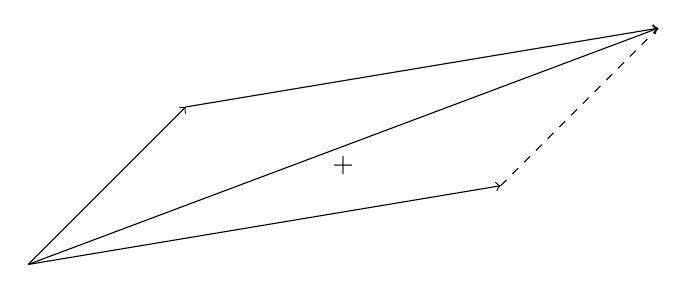
\begin{tikzpicture}
    \coordinate (A) at (0,0);
    \coordinate (B) at (2,2);
    \coordinate (C) at (6,1);
    \coordinate (D) at (8,3);
    \draw[->] (A)--(B) node [left,pos=0.5] {$\bfa$};
    \draw[->] (B)--(D) node [above,pos=0.5] {$\bfb$};
    \draw[->] (A)--(C) node [left,pos=0.5] {$\bfb$};
    \draw[->] (A)--(D) node [below,pos=0.5] {$\bfa+\bfb$};
    \draw[dashed] (C)--(D);
    \end{tikzpicture}
\end{center}
定义向量数乘为实数与向量的运算:\\
有对任意$\lambda\in\R$,则$\lambda\bfa$为大小为$|\lambda||\bfa|$方向为$\sgn(\lambda)\bfa$的向量
\end{dingyi}

\begin{dingli}
在$\R^3$中\\
取直角坐标系$[O;X,Y,Z]$和空间中的向量$\bfa,\bfb,\bfc$\\
则有$\bfa+\bfb=\bfb+\bfa$且$\bfa+(\bfb+\bfc)=(\bfa+\bfb)+\bfc$\\
则有$\bfa+\mathbf{0}=\bfa$且$\bfa+(-\bfa)=\mathbf{0}$\\
则有$|\bfa+\bfb|\leq |\bfa|+|\bfb|$\\
对任意$\lambda,\mu\in\R$\\
则有$\lambda\bfa+\mu\bfa=(\lambda+\mu)\bfa$且$\lambda(\bfa+\bfb)=\lambda\bfa+\mu\bfb$\\
则有$\mu(\lambda\bfa)=(\mu\lambda)\bfa$
\end{dingli}

\begin{dingyi}
在$\R^3$中\\
取直角坐标系$[O;X,Y,Z]$和空间中的向量$\bfa,\bfb$\\
则称向量平移相交后方向夹角为$\bfa,\bfb$的夹角,记为$\langle\bfa,\bfb\rangle\in[0,\pi]$\\
定义向量的内积为向量与向量的运算:\\
有$\bfa\cdot\bfb=|\bfa||\bfb|\cos\langle\bfa,\bfb\rangle$\\
定义向量的外积为向量与向量的运算:\\
有右手螺旋法则:$|\bfa\times\bfb|=|\bfa||\bfb|\sin\langle\bfa,\bfb\rangle,\langle\bfa\times\bfb,\bfa\rangle=\langle\bfa\times\bfb,\bfb\rangle=\frac{\pi}{2}$
\begin{center}
    \begin{tikzpicture}
    \coordinate (O) at (0,0,0);
    \coordinate (A) at (0,0,3);
    \coordinate (B) at (2,0,0);
    \coordinate (C) at (0,2,0);
    \draw[->] (O)--(A) node [left,pos=0.5] {$\bfa$};
    \draw[->] (O)--(B) node [above,pos=0.5] {$\bfb$};
    \draw[->] (O)--(C) node [left,pos=0.5] {$\bfa\times\bfb$};
    \node at (0,0,0) {\Huge\faHandPointRight};
    \end{tikzpicture}
\end{center}
\end{dingyi}

\begin{dingli}
在$\R^3$中\\
取直角坐标系$[O;X,Y,Z]$和空间中的向量$\bfa,\bfb,\bfc$\\
则有$\bfa\cdot\bfb=\bfb\cdot\bfa$且$(\bfa+\bfb)\cdot\bfc=\bfa\cdot\bfc+\bfb\cdot\bfc$\\
则对任意$\lambda\in\R$,有$\lambda(\bfa\cdot\bfb)=(\lambda\bfa)\cdot\bfb$\\
则有$|\bfa\cdot\bfb|\leq|\bfa||\bfb|$\\
则有$\bfa\times\bfb=-\bfb\times\bfa$且$(\bfa+\bfb)\times\bfc=\bfa\times\bfc+\bfb\times\bfc$\\
则对任意$\lambda\in\R$,有$\lambda(\bfa\times\bfb)=(\lambda\bfa)\times\bfb$\\
则有$\bfa\times(\bfb\times\bfc)=(\bfa\cdot\bfc)\bfb-(\bfa\cdot\bfb)\bfc$
\end{dingli}

\begin{dingyi}
在$\R^3$中\\
取直角坐标系$[O;X,Y,Z]$和坐标轴上的单位向量$\bfe_1,\bfe_2,\bfe_3$\\
则有$\bfe_i\cdot\bfe_j=\delta_{ij}$且$\bfe_i\times\bfe_j=\sgn(j-i)\bfe_{6-i-j}$\\
对空间中任意点$P$,有$\overrightarrow{OP}=x\bfe_1+y\bfe_2+z\bfe_3$\\
则称$(x,y,z)$为$\overrightarrow{OP}$的坐标表示,记为$\overrightarrow{OP}=(x,y,z)$
\end{dingyi}

\begin{dingli}
在$\R^3$中\\
取直角坐标系$[O;X,Y,Z]$和向量$\bfa=(x_1,y_1,z_1),\bfb=(x_2,y_2,z_2)$和$\lambda\in\R$\\
则有$\bfa+\bfb=(x_1+x_2,y_1+y_2,z_1+z_2)$且$\lambda\bfa=(\lambda x_1,\lambda x_2,\lambda x_3)$\\
则有$\bfa\cdot\bfb=x_1x_2+y_1y_2+z_1z_2$且$\bfa\times\bfb=(y_1z_2-y_2z_1,z_1x_2-z_2x_1,x_1y_2-x_2y_1)$
\end{dingli}

\chapter{二次曲面}

\begin{dingyi}
在$\R^3$中\\
取直角坐标系$[O;X,Y,Z]$和三元函数$F,F_1,F_2$\\
则称$F(x,y,z)=0$为曲面的一般方程\\
则称$F_1(x,y,z)=F_2(x,y,z)=0$为曲线的一般方程
\end{dingyi}

球面:
\[\frac{x^2}{a^2}+\frac{y^2}{b^2}+\frac{z^2}{c^2}=1\]

\begin{center}
    \begin{minipage}{0.3\textwidth}
        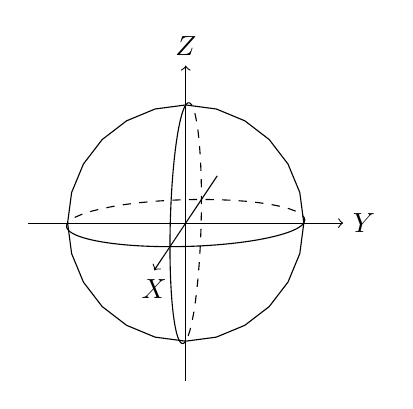
\begin{tikzpicture}[x={(-0.1cm,-0.15cm)},y={(1cm,0cm)},z={(0cm,1cm)}]
        \draw[->] (-4,0,0)--(4,0,0) node[below]{$X$};
        \draw[->] (0,-2,0)--(0,2,0) node[right]{$Y$};
        \draw[->] (0,0,-2)--(0,0,2) node[above]{$Z$};
        \draw plot[domain=0:pi/2] ({2*cos(\x r)},{1.5*sin(\x r)},0);
        \draw[dashed] plot[domain=pi/2:3*pi/2] ({2*cos(\x r)},{1.5*sin(\x r)},0);
        \draw plot[domain=3*pi/2:2*pi] ({2*cos(\x r)},{1.5*sin(\x r)},0);
        \draw plot[domain=0:pi/2] ({2*cos(\x r)},0,{1.5*sin(\x r)});
        \draw[dashed] plot[domain=pi/2:3*pi/2] ({2*cos(\x r)},0,{1.5*sin(\x r)});
        \draw plot[domain=3*pi/2:2*pi] ({2*cos(\x r)},0,{1.5*sin(\x r)});
        \draw plot[domain=0:2*pi] (0,{1.5*cos(\x r)},{1.5*sin(\x r)});
        \end{tikzpicture}
    \end{minipage}
    \hspace{0.5cm}
    \begin{minipage}{0.4\textwidth}
        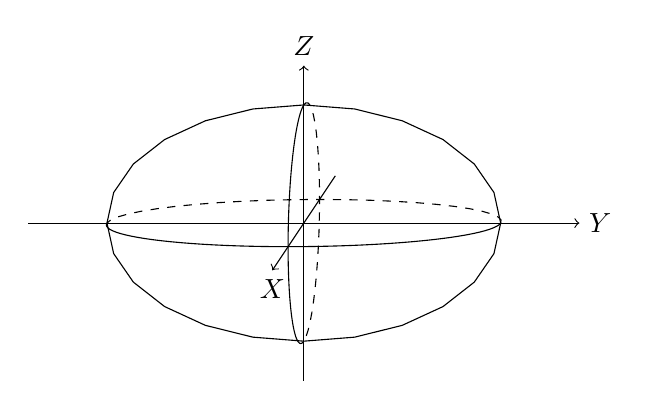
\begin{tikzpicture}[x={(-0.1cm,-0.15cm)},y={(1cm,0cm)},z={(0cm,1cm)}]
        \draw[->] (-4,0,0)--(4,0,0) node[below]{$X$};
        \draw[->] (0,-3.5,0)--(0,3.5,0) node[right]{$Y$};
        \draw[->] (0,0,-2)--(0,0,2) node[above]{$Z$};
        \draw plot[domain=0:pi/2] ({2*cos(\x r)},{2.5*sin(\x r)},0);
        \draw[dashed] plot[domain=pi/2:3*pi/2] ({2*cos(\x r)},{2.5*sin(\x r)},0);
        \draw plot[domain=3*pi/2:2*pi] ({2*cos(\x r)},{2.5*sin(\x r)},0);
        \draw plot[domain=0:pi/2] ({2*cos(\x r)},0,{1.5*sin(\x r)});
        \draw[dashed] plot[domain=pi/2:3*pi/2] ({2*cos(\x r)},0,{1.5*sin(\x r)});
        \draw plot[domain=3*pi/2:2*pi] ({2*cos(\x r)},0,{1.5*sin(\x r)});
        \draw plot[domain=0:2*pi] (0,{2.5*cos(\x r)},{1.5*sin(\x r)});
        \end{tikzpicture}
    \end{minipage}
\end{center}

柱面:
\[F(x,y)=0\]

\begin{center}
    \begin{minipage}{0.2\textwidth}
        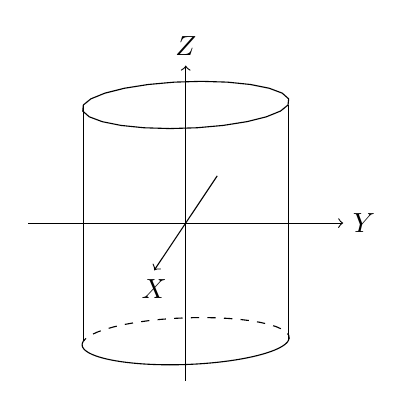
\begin{tikzpicture}[x={(-0.1cm,-0.15cm)},y={(1cm,0cm)},z={(0cm,1cm)}]
        \draw[->] (-4,0,0)--(4,0,0) node[below]{$X$};
        \draw[->] (0,-2,0)--(0,2,0) node[right]{$Y$};
        \draw[->] (0,0,-2)--(0,0,2) node[above]{$Z$};
        \draw plot[domain=0:2*pi] ({2*cos(\x r)},{1.3*sin(\x r)},1.5);
        \draw plot[domain=0:pi/2] ({2*cos(\x r)},{1.3*sin(\x r)},-1.5);
        \draw[dashed] plot[domain=pi/2:3*pi/2] ({2*cos(\x r)},{1.3*sin(\x r)},-1.5);
        \draw plot[domain=3*pi/2:2*pi] ({2*cos(\x r)},{1.3*sin(\x r)},-1.5);
        \draw plot[domain=-1.5:1.5] (0,1.3,{\x});
        \draw plot[domain=-1.5:1.5] (0,-1.3,{\x});
        \end{tikzpicture}
    \end{minipage}
    \hspace{1.5cm}
    \begin{minipage}{0.3\textwidth}
        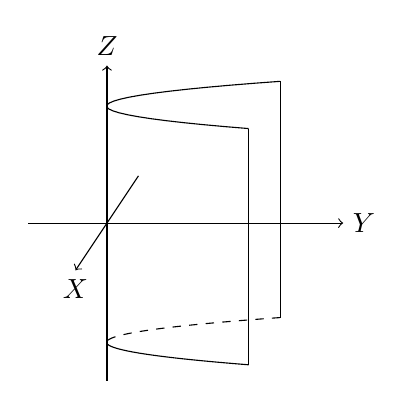
\begin{tikzpicture}[x={(-0.1cm,-0.15cm)},y={(1cm,0cm)},z={(0cm,1cm)}]
        \draw[->] (-4,2,0)--(4,2,0) node[below]{$X$};
        \draw[->] (0,1,0)--(0,5,0) node[right]{$Y$};
        \draw[->] (0,2,-2)--(0,2,2) node[above]{$Z$};
        \draw plot[domain=-2:2] ({\x},{\x*\x/2+2},1.5);
        \draw plot[domain=0:2] ({\x},{\x*\x/2+2},-1.5);
        \draw[dashed] plot[domain=-2:0] ({\x},{\x*\x/2+2},-1.5);
        \draw plot[domain=-1.5:1.5] (0,2,{\x});
        \draw plot[domain=-1.5:1.5] (2,4,{\x});
        \draw plot[domain=-1.5:1.5] (-2,4,{\x});
        \end{tikzpicture}
    \end{minipage}
    \hspace{-0.1cm}
    \begin{minipage}{0.3\textwidth}
        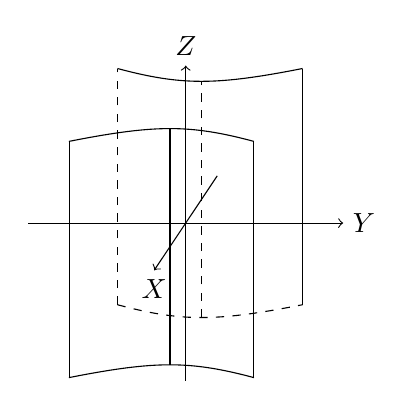
\begin{tikzpicture}[x={(-0.1cm,-0.15cm)},y={(1cm,0cm)},z={(0cm,1cm)}]
        \draw[->] (-4,0,0)--(4,0,0) node[below]{$X$};
        \draw[->] (0,-2,0)--(0,2,0) node[right]{$Y$};
        \draw[->] (0,0,-2)--(0,0,2) node[above]{$Z$};
        \draw plot[domain=-1:1] ({2*cosh(\x)},{sinh(\x)},1.5);
        \draw plot[domain=-1:1] ({-2*cosh(\x)},{sinh(\x)},1.5);
        \draw plot[domain=-1:1] ({2*cosh(\x)},{sinh(\x)},-1.5);
        \draw[dashed] plot[domain=-1:1] ({-2*cosh(\x)},{sinh(\x)},-1.5);
        \draw plot[domain=-1.5:1.5] (3.085,-1.17,{\x});
        \draw plot[domain=-1.5:1.5] (2,0,{\x});
        \draw plot[domain=-1.5:1.5] (3.085,1.17,{\x});
        \draw[dashed] plot[domain=-1.5:1.5] (-3.085,-1.17,{\x});
        \draw[dashed] plot[domain=-1.5:1.5] (-2,0,{\x});
        \draw plot[domain=-1.5:1.5] (-3.085,1.17,{\x});
        \end{tikzpicture}
    \end{minipage}
\end{center}

锥面:
\[F(x,y)=z^2\]

\begin{center}
   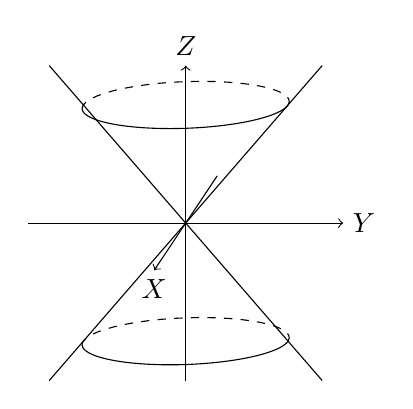
\begin{tikzpicture}[x={(-0.1cm,-0.15cm)},y={(1cm,0cm)},z={(0cm,1cm)}]
    \draw[->] (-4,0,0)--(4,0,0) node[below]{$X$};
    \draw[->] (0,-2,0)--(0,2,0) node[right]{$Y$};
    \draw[->] (0,0,-2)--(0,0,2) node[above]{$Z$};
    \draw plot[domain=0:pi/2] ({2*cos(\x r)},{1.3*sin(\x r)},1.5);
    \draw[dashed] plot[domain=pi/2:3*pi/2] ({2*cos(\x r)},{1.3*sin(\x r)},1.5);
    \draw plot[domain=3*pi/2:2*pi] ({2*cos(\x r)},{1.3*sin(\x r)},1.5);
    \draw plot[domain=0:pi/2] ({2*cos(\x r)},{1.3*sin(\x r)},-1.5);
    \draw[dashed] plot[domain=pi/2:3*pi/2] ({2*cos(\x r)},{1.3*sin(\x r)},-1.5);
    \draw plot[domain=3*pi/2:2*pi] ({2*cos(\x r)},{1.3*sin(\x r)},-1.5);
    \draw plot[domain=-2:2] (0,{1.3*\x/1.5},{\x});
    \draw plot[domain=-2:2] (0,{-1.3*\x/1.5},{\x});
    \end{tikzpicture}
\end{center}

单叶双曲面:
\[\frac{x^2}{a^2}+\frac{y^2}{b^2}-\frac{z^2}{c^2}=1\]

双叶双曲面:
\[\frac{x^2}{a^2}+\frac{y^2}{b^2}-\frac{z^2}{c^2}=-1\]

\begin{center}
    \begin{minipage}{0.4\textwidth}
        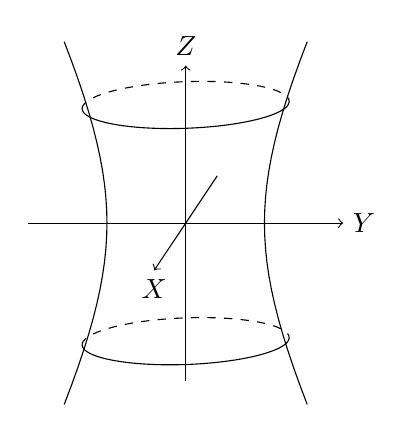
\begin{tikzpicture}[x={(-0.1cm,-0.15cm)},y={(1cm,0cm)},z={(0cm,1cm)}]
        \draw[->] (-4,0,0)--(4,0,0) node[below]{$X$};
        \draw[->] (0,-2,0)--(0,2,0) node[right]{$Y$};
        \draw[->] (0,0,-2)--(0,0,2) node[above]{$Z$};
        \draw plot[domain=0:pi/2] ({2*cos(\x r)},{1.3*sin(\x r)},1.5);
        \draw[dashed] plot[domain=pi/2:3*pi/2] ({2*cos(\x r)},{1.3*sin(\x r)},1.5);
        \draw plot[domain=3*pi/2:2*pi] ({2*cos(\x r)},{1.3*sin(\x r)},1.5);
        \draw plot[domain=0:pi/2] ({2*cos(\x r)},{1.3*sin(\x r)},-1.5);
        \draw[dashed] plot[domain=pi/2:3*pi/2] ({2*cos(\x r)},{1.3*sin(\x r)},-1.5);
        \draw plot[domain=3*pi/2:2*pi] ({2*cos(\x r)},{1.3*sin(\x r)},-1.5);
        \draw plot[domain=-1:1] (0,{cosh(\x)},{1.96*sinh(\x)});
        \draw plot[domain=-1:1] (0,{-cosh(\x)},{1.96*sinh(\x)});
        \end{tikzpicture}
    \end{minipage}
    \hspace{0.5cm}
    \begin{minipage}{0.4\textwidth}
        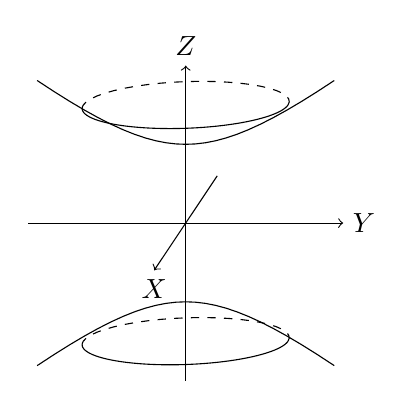
\begin{tikzpicture}[x={(-0.1cm,-0.15cm)},y={(1cm,0cm)},z={(0cm,1cm)}]
        \draw[->] (-4,0,0)--(4,0,0) node[below]{$X$};
        \draw[->] (0,-2,0)--(0,2,0) node[right]{$Y$};
        \draw[->] (0,0,-2)--(0,0,2) node[above]{$Z$};
        \draw plot[domain=0:pi/2] ({2*cos(\x r)},{1.3*sin(\x r)},1.5);
        \draw[dashed] plot[domain=pi/2:3*pi/2] ({2*cos(\x r)},{1.3*sin(\x r)},1.5);
        \draw plot[domain=3*pi/2:2*pi] ({2*cos(\x r)},{1.3*sin(\x r)},1.5);
        \draw plot[domain=0:pi/2] ({2*cos(\x r)},{1.3*sin(\x r)},-1.5);
        \draw[dashed] plot[domain=pi/2:3*pi/2] ({2*cos(\x r)},{1.3*sin(\x r)},-1.5);
        \draw plot[domain=3*pi/2:2*pi] ({2*cos(\x r)},{1.3*sin(\x r)},-1.5);
        \draw plot[domain=-1.2:1.2] (0,{1.25*sinh(\x)},{cosh(\x)});
        \draw plot[domain=-1.2:1.2] (0,{1.25*sinh(\x)},{-cosh(\x)});
        \end{tikzpicture}
    \end{minipage}
\end{center}

椭圆抛物面:
\[\frac{x^2}{a^2}+\frac{y^2}{b^2}=z\]

双曲抛物面:
\[\frac{x^2}{a^2}-\frac{y^2}{b^2}=z\]

\begin{center}
   \begin{minipage}{0.4\textwidth}
        \begin{tikzpicture}[x={(-0.1cm,-0.15cm)},y={(1cm,0cm)},z={(0cm,1cm)}]
        \draw[->] (-4,0,0)--(4,0,0) node[below]{$X$};
        \draw[->] (0,-2,0)--(0,2,0) node[right]{$Y$};
        \draw[->] (0,0,-2)--(0,0,2) node[above]{$Z$};
        \draw plot[domain=0:pi/2] ({2*cos(\x r)},{1.3*sin(\x r)},1.5);
        \draw[dashed] plot[domain=pi/2:3*pi/2] ({2*cos(\x r)},{1.3*sin(\x r)},1.5);
        \draw plot[domain=3*pi/2:2*pi] ({2*cos(\x r)},{1.3*sin(\x r)},1.5);
        \draw plot[domain=-1.5:1.5] (0,{\x},{0.887*\x*\x});
        \end{tikzpicture}
    \end{minipage}
    \hspace{0.5cm}
    \begin{minipage}{0.4\textwidth}
        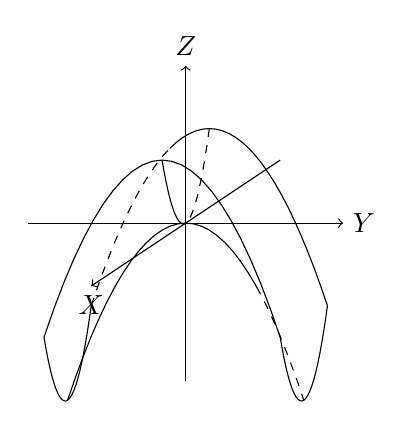
\begin{tikzpicture}[x={(-0.3cm,-0.2cm)},y={(1cm,0cm)},z={(0cm,1cm)}]
        \draw[->] (-4,0,0)--(4,0,0) node[below]{$X$};
        \draw[->] (0,-2,0)--(0,2,0) node[right]{$Y$};
        \draw[->] (0,0,-2)--(0,0,2) node[above]{$Z$};
        \draw[dashed] plot[domain=-1:0] ({\x},0,{\x*\x});
        \draw plot[domain=0:1] ({\x},0,{\x*\x});
        \draw[dashed] plot[domain=-1.5:-0.5] (-1,{\x},{1-\x*\x});
        \draw plot[domain=-0.5:1.5] (-1,{\x},{1-\x*\x});
        \draw plot[domain=-1.5:1.5] (1,{\x},{1-\x*\x});
        \draw plot[domain=-1:1] ({\x},1.5,{\x*\x-2.25});
        \draw plot[domain=-1:1] ({\x},-1.5,{\x*\x-2.25});
        \draw plot[domain=-1.5:0.9] (0,{\x},{-\x*\x});
        \draw[dashed] plot[domain=0.9:1.5] (0,{\x},{-\x*\x});
        \end{tikzpicture}
    \end{minipage}
\end{center}

\chapter{一些变换}

\begin{dingyi}
在$\R^3$中\\
取直角坐标系$[O;X,Y,Z]$和$\overrightarrow{OP}=x\bfe_1+y\bfe_2+z\bfe_3$\\
考虑另一直角坐标系$[O';X',Y',Z']$和$\overrightarrow{O'P}=x'\bfe_1'+y'\bfe_2'+z'\bfe_3'$\\
在$[O;X,Y,Z]$上,记$O',\bfe_i'$的坐标为$(a_1,a_2,a_3),(a_{1i},a_{2i},a_{3i})$\\
则称$\overrightarrow{OP}=\sum\limits_{i=1}^{3}(a_i+\sum\limits_{j=1}^{3}a_{ij})\bfe_i$为$[O;X,Y,Z],[O';X',Y',Z']$的坐标变换公式
\end{dingyi}

\begin{dingyi}
在$\R^3$中\\
若有$\varphi$为空间中点到点的一一对应,则称$\varphi$为变换,则称$\varphi^{-1}$为$\varphi$的逆变换
\end{dingyi}

\begin{dingli}
在$\R^3$中\\
对任意变换$\varphi,\psi,\tau$,则有$\tau\circ(\psi\circ\varphi)=(\tau\circ\psi)\circ\varphi$且$\varphi\circ\id=\varphi$\\
则有存在唯一变换$\varphi^{-1}$,有$\varphi\circ\varphi^{-1}=\varphi^{-1}\circ\varphi=\id$
\end{dingli}

\begin{dingyi}
在$\R^3$中\\
若有变换$\alpha$,对空间中任意点$P$,有$\overrightarrow{P\alpha(P)}$为常向量$\bfa$\\
则称$\alpha$为平移变换\\
则称$\overrightarrow{O\alpha(P)}=\bfa+\overrightarrow{OP}$为平移变换的坐标公式\\
若有变换$\tau$,存在点$P_0$和$\theta\in[0,2\pi)$\\
对任意点$P\in\overline{OP_0}$,有$\tau(P)=P$\\
对任意点$P\notin\overline{OP_0}$,有$\langle\overrightarrow{OP_0}\times\overrightarrow{OP},\overrightarrow{OP_0}\times\overrightarrow{O\tau(P)}\rangle=\theta$\\
则称$\tau$为旋转变换,则称$\overline{OP}$为旋转轴,则称$\theta$为旋转角,记$\bfe=\frac{\overrightarrow{OP_0}}{|OP_0|}$\\
则称$\overrightarrow{O\tau(P)}=(1-\cos\theta)(\bfe\cdot\overrightarrow{OP})\bfe+\cos\theta\overrightarrow{OP}+\sin\theta\bfe\times\overrightarrow{OP}$为旋转变换的坐标公式\\
若有变换$\pi$,存在法向量$\mathbf{n}$确定的过原点平面$\beta$\\
对任意点$P\in\beta$,有$\pi(P)=P$\\
对任意点$P\notin\beta$,有$\overrightarrow{\pi(P)P}\neq\mathbf{0}$且$\overrightarrow{\pi(P)P}\cdot\mathbf{n}=0$且$\overrightarrow{O\pi(P)}\times\mathbf{n}=\overrightarrow{OP}\times\mathbf{n}$\\
则称$\pi$为反射变换,则称$\beta$为反射平面\\
则称$\overrightarrow{O\pi(P)}=\overrightarrow{OP}-2(\overrightarrow{OP}\cdot\mathbf{n})\mathbf{n}$为反射变换的坐标公式\\
若有变换$\varphi$,对空间中任意点$P_1,P_2$,有$|\varphi(P_1)\varphi(P_2)|=|P_1P_2|$\\
则称$\varphi$为正交变换
\end{dingyi}

%\begin{zhu}
%$\overrightarrow{O\tau(P)}=(\bfe\cdot\overrightarrow{OP})\bfe+\cos\theta(\overrightarrow{OP}-(\bfe\cdot\overrightarrow{OP})\bfe)+\sin\theta\bfe\times(\overrightarrow{OP}-(\bfe\cdot\overrightarrow{OP})\bfe)$
%\end{zhu}

\begin{dingli}
在$\R^3$中\\
对任意正交变换$\varphi$,存在平移变换$\alpha$,旋转变换$\tau$,反射变换$\pi$,有$\varphi=\pi\circ\tau\alpha$\\
其中平移变换,旋转变换,反射变换可为$\id$
\end{dingli}

\begin{zhu}
以下用坐标方程组来描述上述变换:\\
对$[O;X,Y,Z],[O';X',Y',Z']$的坐标变换:
\[\begin{cases*}x=a_1+a_{11}x'+a_{12}y'+a_{13}z'\\y=a_2+a_{21}x'+a_{22}y'+a_{23}z'\\z=a_3+a_{31}x'+a_{32}y'+a_{33}z'\end{cases*}\]
有正交条件:
\[\begin{cases*}a_{11}^2+a_{21}^2+a_{31}^2=a_{12}^2+a_{22}^2+a_{32}^2=a_{13}^2+a_{23}^2+a_{33}^2=1\\a_{11}a_{12}+a_{21}a_{22}+a_{31}a_{32}=a_{12}a_{13}+a_{22}a_{23}+a_{32}a_{33}=a_{13}a_{11}+a_{23}a_{21}+a_{33}a_{31}=0\end{cases*}\]
对向量$\bfa=(a_1,a_2,a_3)$的平移变换:
\[\begin{cases*}x'=x+a_1\\y'=y+a_2\\z'=z+a_3\end{cases*}\]
对旋转轴$x=y=0$旋转角$\theta$的平移变换:
\[\begin{cases*}x'=x\cos\theta-y\sin\theta\\y'=x\sin\theta+y\cos\theta\\z'=z\end{cases*}\]
对法向量$(0,0,1)$的反射变换:
\[\begin{cases*}x'=x\\y'=y \\z'=-z\end{cases*}\]
对正交变换:
\[\begin{cases*}x'=a_1+a_{11}x+a_{12}y+a_{13}z\\y'=a_2+a_{21}x+a_{22}y+a_{23}z\\z'=a_3+a_{31}x+a_{32}y+a_{33}z\end{cases*}\]
有正交条件且$\left|\begin{matrix*}a_{11}&a_{12}&a_{13}\\a_{21}&a_{22}&a_{23}\\a_{31}&a_{32}&a_{33}\end{matrix*}\right|=1$
\end{zhu}

%\end{document}

\part{\kaishu 范畴理论}

%\documentclass[12pt,oneside,a4paper]{book}

%\usepackage{amsmath}
%\usepackage{mathtools}
%\usepackage{amsfonts}
%\usepackage{unicode-math}
%\usepackage{geometry}
%\usepackage{ctex}

%\begin{document}

%\setcounter{chapter}{0}
\setcounter{section}{0}
\setcounter{subsection}{0}

\begin{dingyi}
对一个集合和集合上的关系$\mcc$\\
记其包含的元素集为$\Obj(\mcc)$,对任意$X,Y\in \Obj(\mcc)$,有态射集$\Hom_{\mcc}(X,Y)\in\mcc$\\
有$\id_{X}\in \Hom_{\mcc}(X,X)$且$\Hom_{\mcc}(X,Y)\times\Hom_{\mcc}(Y,Z)\to \Hom_{\mcc}(X,Z),(f,g)\mapsto g\circ f$\\
则称$\mcc$为一个范畴
\end{dingyi}

\begin{dingyi}
对范畴$\mcc$\\
对$f\in\Hom_{\mcc}(X,Y),g\in\Hom_{\mcc}(Y,X)$,有$f\circ g=\id_{Y}$且$g\circ f=\id_{X}$\\
则称$f,g$互为逆态射,记为$g=f^{-1}$\\
对$f\in\Hom_{\mcc}(X,Y)$,存在$g\in\Hom_{\mcc}(Y,X)$,有$g=f^{-1}$\\
则称$f$为同构态射\\
对$X,Y\in\Obj(\mcc)$,存在$f\in\Hom_{\mcc}(X,Y)$为同构态射\\
则称$X,Y$互为同构,记为$X\cong_{\mcc} Y$
\end{dingyi}

\begin{dingyi}
对范畴$\mcc$和$\mcd$\\
考虑一个态射$F:\mcc\to\mcd$\\
对任意$X\in\Obj(\mcc),\Hom_{\mcc}(X_1,X_2)\in\mcc$\\
有$F(X)\in\Obj(\mcd),\Hom_{\mcd}(F(X_1),F(X_2))\in \mcd$且$F(\id_{X})=\id_{F(X)}$\\
对任意$f\in \Hom_{\mcc}(X_1,X_2),g\in \Hom_{\mcc}(X_2,X_3)$,有$F(g)\circ F(f)=F(g\circ f)\in \Hom_{\mcd}(F(X_1),F(X_3))$\\
则称$F$为$\mcc\to\mcd$的函子,记为$F:\mcc\to\mcd$\\
对任意$X\in\Obj(\mcc),\Hom_{\mcc}(X_1,X_2)\in\mcc$\\
有$F(X)\in\Obj(\mcd),\Hom_{\mcd}(F(X_2),F(X_1))\in \mcd$且$F(\id_{X})=\id_{F(X)}$\\
对任意$f\in \Hom_{\mcc}(X_1,X_2),g\in \Hom_{\mcc}(X_2,X_3)$,有$F(f)\circ F(g)=F(g\circ f)\in \Hom_{\mcd}(F(X_3),F(X_1))$\\
则称$F$为$\mcc\to\mcd$的反变函子,记为$F:\mcc^{op}\to\mcd$
\end{dingyi}

\begin{dingli}
对范畴$\mcc$和$\mcd$和函子$F:\mcc\to\mcd$\\
对$X,Y\in\Obj(\mcc)$,若$X\cong_{\mcc}Y$,则$F(X)\cong_{\mcd}F(Y)$
\end{dingli}

\begin{dingyi}
对范畴$\mcc$和$\mcd$和函子$F:\mcc\to\mcd$\\
对任意$X,Y\in \mcc$,有$\Hom_{\mcc}(X,Y)\to\Hom_{\mcd}(F(X),F(Y)),f\mapsto F(f)$为满射\\
则称$F$为全的\\
对任意$X,Y\in \mcc$,有$\Hom_{\mcc}(X,Y)\to\Hom_{\mcd}(F(X),F(Y)),f\mapsto F(f)$为单射\\
则称$F$为忠实的\\
对任意$X,Y\in \mcc$,若$F(f)\in\Hom_{\mcd}(F(X),F(Y))$为同构态射,有$f\in\Hom_{\mcc}(X,Y)$为同构态射\\
则称$F$为保守的\\
对任意$X,Y\in \mcc$,若$F(X)=F(Y)$,则$X=Y$\\
则称$F$为单的\\
对任意$X'\in \mcd$,存在$X\in \mcc$,有$F(X)=X'$\\
则称$F$为满的\\
对任意$X'\in \mcd$,存在$X\in \mcc$,有$F(X)\cong_{\mcd} X'$\\
则称$F$为本质满的
\end{dingyi}

\begin{dingyi}
对范畴$\mcc$和$\mcd$\\
对$F,G:\mcc\to\mcd$为函子,若有$\eta:F\to G$,对任意$X\in\mcc,f\in\Hom_{\mcc}(X_1,X_2)$\\
有$\eta_{X}\in\Hom_{\mcd}(F(X),G(X))$且$\eta_{X_2}\circ F(f)=G(f)\circ\eta_{X_1}$\\
则称$\eta$为$F\to G$的自然变换\\
考虑一个范畴$\Fun(\mcc,\mcd)$\\
有任意$F\in\Obj(\Fun(\mcc,\mcd))$为$\mcc\to\mcd$的函子\\
对任意$F,G\in\Obj(\Fun(\mcc,\mcd))$,有任意$\eta\in\Hom(F,G)$为$F\to G$的自然变换\\
则称$\Fun(\mcc,\mcd)$为$\mcc\to \mcd$的函子范畴\\
对$F,G\in\Obj(\Fun(\mcc,\mcd))$,存在$\eta\in\Hom_{\Fun(\mcc,\mcd)}(F,G),\sigma\in\Hom_{\Fun(\mcc,\mcd)}(G,F)$\\
有$\eta\circ\sigma=\id_{F}$且$\sigma\circ\eta=\id_{G}$,即对任意$X\in\mcc$,有$\eta_{X}\circ\sigma_{X}=\id_{F(X)}$且$\sigma_{X}\circ\eta_{X}=\id_{G(X)}$\\
则称$F,G$互为同构,记为$F\cong_{\Fun(\mcc,\mcd)}G$
\end{dingyi}

\begin{dingyi}
对范畴$\mcc$和$\mcd$和函子$F:\mcc\to\mcd$\\
若对$F:\mcc\to\mcd$,存在$G:\mcd\to\mcc$,有$G\circ F=\id_{\mcc}$且$F\circ G=\id_{\mcd}$\\
则称$F$为范畴同构,即全忠实且单且满\\
若对$F:\mcc\to\mcd$,存在$G:\mcd\to\mcc$,有$G\circ F\cong_{\Fun(\mcc,\mcc)}\id_{\mcc}$且$F\circ G\cong_{\Fun(\mcd,\mcd)}\id_{\mcd}$\\
则称$F$为范畴等价,即全忠实且本质满
\end{dingyi}

\begin{zhu}
范畴等价的直观:\\
每个对象在对方范畴内有同构的对象,态射通过诱导得到模去同构的双射
\end{zhu}

\begin{dingyi}
对范畴$\mcc$\\
若$\Obj(\mcc)$和$\{\Hom_{\mcc}\}$为集合,则称$\mcc$为小范畴\\
若$\mcc$范畴等价于一个小范畴,则称$\mcc$为本质小范畴
\end{dingyi}

\begin{dingyi}
对小范畴$\mcc$和范畴$\mcd$,有函子$F:\mcc \to \mcd$\\
则称$F$为$\mcd$中的$\mcc$-图表\\
若对$X_i,X_j\in\Obj(\mcc),Y\in\Obj(\mcd)$,存在$\varphi:Y\to\mcc$,对任意$f_{ij}\in\Hom_{\mcc}(X_i,X_j)$\\
有$\varphi_{i}:Y\to F(X_{i})$且$\varphi_{j}=F(f_{ij})\circ\varphi_{i}$,即下面图表交换:
\begin{center}
    $\begin{tikzcd}
    & Y \ar[dl,"\varphi_{i}"'] \ar[dr,"\varphi_{j}"'] & \\
    F(X_i) \ar[rr,"F(f_{ij})"] & & F(X_j)
    \end{tikzcd}$
\end{center}
则称$(Y,\varphi)$为$\mcc$-图表的锥\\
若对$X_i,X_j\in\Obj(\mcc),Y\in\Obj(\mcd)$,存在$\varphi:\mcc\to Y$,对任意$f_{ij}\in\Hom_{\mcc}(X_i,X_j)$\\
有$\varphi_{i}:F(X_{i})\to Y$且$\varphi_{i}=\varphi_{j}\circ F(f_{ij})$,即下面图表交换:
\begin{center}
    $\begin{tikzcd}
    F(X_i) \ar[rr,"F(f_{ij})"] \ar[dr,"\varphi_{i}"'] & & F(X_j) \ar[dl,"\varphi_{j}"'] \\
    & Y &
    \end{tikzcd}$
\end{center}
则称$(Y,\varphi)$为$\mcc$-图表的余锥
\end{dingyi}

\begin{dingyi}
对小范畴$\mcc$和范畴$\mcd$,有函子$F:\mcc \to \mcd$\\
若存在$(Z,\psi)$为$\mcc$-图表的锥,对任意$(Y,\varphi)$为$\mcc$-图表的锥\\
存在唯一态射$h:Y\to Z$,对任意$X_i\in\Obj(\mcc)$,有$\varphi_{i}=\psi_{i}\circ h$,即下面图表交换:
\begin{center}
    $\begin{tikzcd}
     & Y \ar[ddl,"\varphi_{i}"'] \ar[d,dashed,"h"'] \ar[ddr,"\varphi_{j}"] & \\
     & Z \ar[dl,"\psi_{i}"] \ar[dr,"\psi_{j}"'] & \\
    F(X_{i}) \ar[rr,"F(f_{ij})"'] &  &  F(X_{j})
    \end{tikzcd}$
\end{center}
则称$(Z,\psi)$为$F$的极限,记为$\lim\limits_{X\in\mcc}F(X)$\\
若存在$(Z,\psi)$为$\mcc$-图表的余锥,对任意$(Y,\varphi)$为$\mcc$-图表的余锥\\
存在唯一态射$h:Z\to Y$,对任意$X_i\in\Obj(\mcc)$,有$\varphi_{i}=h\circ\psi_{i}$,即下面图表交换:
\begin{center}
    $\begin{tikzcd}
    F(X_{i}) \ar[rr,"F(f_{ij})"] \ar[dr,"\psi_{i}"] \ar[ddr,"\varphi_{i}"'] &  & F(X_{j}) \ar[dl,"\psi_{j}"'] \ar[ddl,"\varphi_{j}"'] \\
     & Z \ar[d,dashed,"h"] & \\
     & Y & 
    \end{tikzcd}$
\end{center}
则称$(Z,\psi)$为$F$的余极限,记为$\colim\limits_{X\in\mcc}F(X)$
\end{dingyi}

\begin{dingli}
对小范畴$\mcc$和范畴$\mcd$,有函子$F:\mcc \to \mcd$\\
若$(U,\varphi),(V,\psi)$为$F$的极限,则$U\cong_{\mcd}V$\\
若$(U,\varphi),(V,\psi)$为$F$的余极限,则$U\cong_{\mcd}V$
\end{dingli}

\begin{zhu}
以下为集合范畴的重要例子:\\
考虑一组集合$X_{i}$和投射$\varphi_{i}:X_{i+1}\to X_{i}$\\
此映射链构成交换图表: $X_1\stackrel{\varphi_{1}}{\leftarrow}X_2\stackrel{\varphi_{2}}{\leftarrow}X_3\stackrel{\varphi_{3}}{\leftarrow}\cdots$\\
则一定存在锥构成序列的反极限$($对应范畴中的极限$)$,即下面图表交换:
\begin{center}
    $\begin{tikzcd}
     & & \lim\limits_{\leftarrow}X_i \ar[dll,"\psi_1"'] \ar[dl,"\psi_2"',pos=0.8] \ar[d,"\psi_3"'] & \\
    X_1 & X_2 \ar[l,"\varphi_{1}"] & X_3 \ar[l,"\varphi_{2}"] & \cdots \ar[l,"\varphi_{3}"]
    \end{tikzcd}$
\end{center}
考虑一组集合$X_{i}$和包含$\varphi_{i}:X_{i}\to X_{i+1}$\\
此映射链构成交换图表: $X_1\stackrel{\varphi_{1}}{\rightarrow}X_2\stackrel{\varphi_{2}{\rightarrow}}X_3\stackrel{\varphi_{3}}{\rightarrow}\cdots$\\
则一定存在余锥构成序列的正极限$($对应范畴中的余极限$)$,即下面图表交换:
\begin{center}
    $\begin{tikzcd}
    X_1 \ar[r,"\varphi_{1}"] \ar[drr,"\psi_1"'] & X_2 \ar[r,"\varphi_{2}"] \ar[dr,"\psi_2"',pos=0.05] & X_3 \ar[r,"\varphi_{3}"] \ar[d,"\psi_3"'] & \cdots\\
     & & \lim\limits_{\rightarrow}X_i & 
    \end{tikzcd}$
\end{center}
\end{zhu}

\begin{dingyi}
对小范畴$\mcc$和范畴$\mcd$,有函子$F:\mcc \to \mcd$\\    
若$\mcc$为偏序集$(X_i,\leq)\ ($偏序即为态射$)$且$\mcd$为Abel范畴\\
有$(Z,\varphi)$为$F$的余极限且$Z$满足以下两条性质:\\
对$y_i\in F(X_i)$,若有$\varphi_{i}(y_{i})=0\in Z$,则存在$X_i\leq X_j$,有$F(f_{ij})(d_i)=0$\\
对$X_i\leq X_j$,若有任意$F(f_{ij})$为单射,则诱导典范态射$\lim\limits_{\rightarrow}X_{i}\to Z$为单射\\
则称$(Z,\varphi)$为$F$的滤余极限
\end{dingyi}

\begin{dingli}
Yoneda引理:\\
对小范畴$\mcc$,有函子范畴$\Fun(\mcc^{op},Sets)$\\
有函子$\mathrm{y}:\mcc\to\Fun(\mcc^{op},Sets)$为Yoneda嵌入\\
有$X\mapsto h_{X}=\Hom_{\mcc}(-,X)$且$f:X\to Y\mapsto \Hom_{\mcc}(-,X)\to\Hom_{\mcd}(-,Y)$\\
则$\mathrm{y}$为忠实的且有同构$\Hom_{\Fun(\mcc^{op},Sets)}(h_{X},F)\cong F(X)$\\
其中$X\in \mcc$且$F\in\Fun(\mcc^{op},Sets)$,则$\mathrm{y}(X)=h_{X}\in \Fun(\mcc^{op},Sets)$且$F(X)\in Sets$
\end{dingli}

%\end{document}

\part{\kaishu 线性代数}

%\documentclass[12pt,oneside,a4paper]{book}

%\usepackage{amsmath}
%\usepackage{mathtools}
%\usepackage{amsfonts}
%\usepackage{unicode-math}
%\usepackage{geometry}
%\usepackage{ctex}

%\begin{document}

%\setcounter{chapter}{0}
\setcounter{section}{0}
\setcounter{subsection}{0}

\chapter{线性方程}

\begin{dingyi}
对数域$K$\\
若有$a_{ij}\in K,b_{i}\in K$\\
则称$\begin{cases}a_{11}x_1+a_{12}x_2+\cdots+a_{1n}x_n=b_1\\ a_{21}x_1+a_{22}x_2+\cdots+a_{2n}x_n=b_2\\ \cdots\\ a_{m1}x_1+a_{m2}x_2+\cdots+a_{mn}x_n=b_n\end{cases}$为$n$元线性方程组\\
若有$(x_1,x_2,\cdots,x_n)^{T}\in K^n$满足上述方程\\
则称$(x_1,x_2,\cdots,x_n)^{T}$为$n$元线性方程组的解\\
则称$\{\alpha\in K^n|\alpha\text{为}n\text{元线性方程组的解}\}$为解集\\
若有变换:一方程乘常数加至另一方程/互换一方程与另一方程位置/非零数乘至一方程\\
则称上述变换为$n$元线性方程组的初等变换
\end{dingyi}

\begin{dingli}
对数域$K$\\
则$n$元线性方程组的初等变换不改变$n$元线性方程组的解集
\end{dingli}

\begin{dingyi}
对数域$K$\\
若有$a_{ij}\in K$,其中$i\in\{1,2,\cdots,m\},j\in\{1,2,\cdots,n\}$\\
则称$A=\begin{bmatrix}a_{11} & a_{12} & \cdots & a_{1n}\\ a_{21} & a_{22} & \cdots & a_{2n}\\ \vdots & \vdots & \ddots & \vdots\\ a_{m1} & a_{m2} & \cdots & a_{mn} \end{bmatrix}$为$K$上$m\times n$矩阵,记为$A=(a_{ij}),A(i:j)=a_{ij}$\\
则称$K_{m\times n}=\{A|A\text{为}K\text{上}m\times n\text{矩阵}\}$为$K$上$m\times n$矩阵空间\\
若对$A\in K_{m\times n}$,存在$c_{1},\cdots,c_{m}\in \{1,\cdots,n\}$\\
有$c_{1}\leq c_{2}\leq \cdots\leq c_{m}$,若$c_{i}=c_{i+1}$,则$c_{i}=c_{i+1}=\cdots=c_{n}=n$\\
有对任意$i\in\{1,\cdots,m\}$,对任意$1\leq k \leq c_{i}$,有$A(i:k)=0$且$A(i:c_{i}+1)\neq 0$\\
则称$A$为行阶梯型矩阵\\
若对$A\in K_{m\times n}$为行阶梯型矩阵,有$A(i:c_{i}+1)=1$\\
则称$A$为简化行阶梯型矩阵\\
\ \\
若有变换:一行乘常数加至另一行/互换一行与另一行位置/取合适非零数乘在一行上\\
则称上述变换为矩阵的初等行变换\\
若对$A\in K_{m\times n}$,存在$c_{1},\cdots,c_{n}\in \{1,\cdots,m\}$\\
有$c_{1}\leq c_{2}\leq \cdots\leq c_{n}$,若$c_{i}=c_{i+1}$,则$c_{i}=c_{i+1}=\cdots=c_{n}=m$\\
有对任意$j\in\{1,\cdots,n\}$,对任意$1\leq k \leq c_{j}$,有$A(k:j)=0$且$A(c_{j}+1:j)\neq 0$\\
则称$A$为行阶梯型矩阵\\
若对$A\in K_{m\times n}$为行阶梯型矩阵,有$A(j:c_{j}+1)=1$\\
则称$A$为简化行阶梯型矩阵\\
若有变换:一列乘常数加至另一列/互换一列与另一列位置/取合适非零数乘在一列上\\
则称上述变换为矩阵的初等列变换
\end{dingyi}

\begin{dingli}
对数域$\R$\\
则任意$A\in \R_{m\times n}$均可做初等行变换得到简化行阶梯型矩阵
\end{dingli}

\begin{dingyi}
对数域$K$\\
若有$n$元线性方程组$\begin{cases}a_{11}x_1+a_{12}x_2+\cdots+a_{1n}x_n=b_1\\ a_{21}x_1+a_{22}x_2+\cdots+a_{2n}x_n=b_2\\ \cdots\\ a_{m1}x_1+a_{m2}x_2+\cdots+a_{mn}x_n=b_n\end{cases}$为$n$元线性方程组\\
则称$\begin{bmatrix}a_{11} & a_{12} & \cdots & a_{1n} \\ a_{21} & a_{22} & \cdots & a_{2n} \\ \vdots & \vdots & \ddots & \vdots \\ a_{m1} & a_{m2} & \cdots & a_{mn}\end{bmatrix}$为$n$元线性方程组的系数矩阵\\
则称$\begin{bmatrix}a_{11} & a_{12} & \cdots & a_{1n} & b_1\\ a_{21} & a_{22} & \cdots & a_{2n} & b_2\\ \vdots & \vdots & \ddots & \vdots & \vdots\\ a_{m1} & a_{m2} & \cdots & a_{mn} & b_m\end{bmatrix}$为$n$元线性方程组的增广矩阵\\
若对增广矩阵做初等行变换得到简化行阶梯型矩阵以此得到方程的解\\
则称上述方法为Gauss消元法
\end{dingyi}

\begin{zhu}
对增广矩阵做初等行变换等价于对线性方程组做初等变换
\end{zhu}

\begin{dingli}
对数域$K$\\
若$K=\Q$或$\R$或$\C$,则$n$元线性方程组的解仅有三种可能:无解/唯一解/无穷多解\\
则$n$元线性方程组无解当且仅当\\
系数矩阵和增广矩阵做初等行变换得到简化行阶梯型矩阵非零行数不同\\
则$n$元线性方程组有唯一解当且仅当\\
系数矩阵和增广矩阵做初等行变换得到简化行阶梯型矩阵非零行数相同且为$n$\\
则$n$元线性方程组有无穷多解当且仅当\\
系数矩阵和增广矩阵做初等行变换得到简化行阶梯型矩阵非零行数相同且小于$n$
\end{dingli}

\begin{dingyi}
对数域$K$\\
若有$a_{ij}\in K$\\
则称$\begin{cases}a_{11}x_1+a_{12}x_2+\cdots+a_{1n}x_n=0\\ a_{21}x_1+a_{22}x_2+\cdots+a_{2n}x_n=0\\ \cdots\\ a_{m1}x_1+a_{m2}x_2+\cdots+a_{mn}x_n=0\end{cases}$为$n$元齐次线性方程组\\
则称$(0,0,\cdots,0)^{T}$为$n$元齐次线性方程组的零解,则称其他的解为非零解
\end{dingyi}

\begin{dingli}
对数域$K$\\
则$n$元齐次线性方程组有非零解当且仅当\\
系数矩阵做初等行变换得到简化行阶梯型矩阵非零行数小于$n$
\end{dingli}

\begin{dingyi}
对数域$K$\\
若有$A\in K_{m\times n}$做初等行变换得到简化行阶梯型矩阵的非零行数为$r_{r}(A)$\\
则称$r_{r}(A)$为$A$的行秩\\
若有$A\in K_{m\times n}$做初等列变换得到简化列阶梯型矩阵的非零列数为$r_{c}(A)$\\
则称$r_{c}(A)$为$A$的列秩
\end{dingyi}

\begin{dingli}
对数域$K$\\
若有$A\in K_{m\times n}$做初等行变换得到$B\in K_{m\times n}$\\
则$r_{r}(A)=r_{r}(B)$且$r_{c}(A)=r_{c}(B)$
\end{dingli}

\begin{dingli}
对数域$K$\\
若有$A\in K_{m\times n}$,则$r_{r}(A)=r_{c}(A)$\\
则称$\rank(A)=r_{r}(A)=r_{c}(A)$为$A$的秩
\end{dingli}

\begin{dingli}
对数域$K$\\
则$n$元线性方程组无解当且仅当$\rank(\text{系数矩阵})\neq\rank(\text{增广矩阵})$\\
则$n$元线性方程组有唯一解当且仅当$\rank(\text{系数矩阵})=\rank(\text{增广矩阵})=n$\\
则$n$元线性方程组有无穷多解当且仅当$\rank(\text{系数矩阵})=\rank(\text{增广矩阵})<n$\\
则$n$元齐次线性方程组有非零解当且仅当$\rank(\text{系数矩阵})<n$
\end{dingli}

\begin{dingyi}
对数域$K$\\
若有$A=(a_{ij})\in K_{m\times n},B=(b_{ij})\in K_{m\times n},k\in K$\\
定义矩阵加法:$A+B=(a_{ij}+b_{ij})\in K_{m\times n}$\\
定义矩阵数乘:$kA=(ka_{ij})\in K_{m\times n}$\\
则称$-A=-1A$为$A$的负矩阵,则称$0A$为零矩阵,记为$\bf0$
\end{dingyi}

\begin{dingli}
对数域$K$\\
若有$A,B,C\in K_{m\times n},k,l\in K$\\
则$A+B=B+A$且$(A+B)+C=A+(B+C)$且$A+{\bf0}=A$且$A+(-A)={\bf0}$\\
则$(kl)A=k(lA)$且$(k+l)A=kA+lA$且$k(A+B)=kA+kB$
\end{dingli}

\begin{dingyi}
对数域$K$\\
若有$A=(a_{ik})\in K_{m\times l},B=(b_{kj})\in K_{l\times n}$\\
定义矩阵乘法:$AB=(\sum\limits_{k=1}^{l}a_{ik}b_{kj})\in K_{m\times n}$\\
则称$I=(\iota_{ij})\in K_{m\times n}$为单位矩阵,其中$\iota_{ij}=1,i=j ;\iota_{ij}=0,i\neq j$\\
若$AB=BA$,则称$A,B$可交换
\end{dingyi}

\begin{dingli}
对数域$K$\\
若有$A,B,C\in K_{*\times *},I\in K_{*\times *},k\in K$\\
则$(AB)C=A(BC)$且$A(B+C)=AB+AC$且$(A+B)C=AC+BC$\\
则$IA=AI=A$且$k(AB)=(kA)B=A(kB)$且$(kI)A=kA$
\end{dingli}

\begin{dingyi}
对数域$K$\\
若有$A=(a_{ij}),B=(b_{ij})\in K_{n\times n}$\\
定义矩阵幂乘:$A^{m}=AA\cdots A$,其中$m\in \N^*$,记$A^{0}=I\in K_{n\times n}$\\
若有$A=(a_{ij})\in K_{n\times n}$且存在$k\in \N^*$,有$A^k={\bf0}$,则称$A$为幂零矩阵
\end{dingyi}

\begin{dingli}
对数域$K$\\
若有$A,B\in K_{n\times n},I\in K_{n\times n},k\in K,m,l\in \N$\\
则$A^{m}A^{l}=A^{m+l}$且$(A^{m})^{l}=A^{ml}$且$A,kI$可交换\\
若有$A,B$可交换,则$(A+B)^{m}=\sum\limits_{i=0}^{n}C_{n}^{i}A^{i}B^{n-i}$
\end{dingli}

\begin{dingyi}
对数域$K$\\
若有$f:K_{n\times n}\to K, \lambda\in K$\\
有$f(\begin{bmatrix}a_{11} & a_{12} & \cdots & a_{1n} \\ \vdots & \vdots & \vdots & \vdots \\ a_{i1}+b_{i1} & a_{i2}+b_{i2} & \cdots & a_{in}+b_{in}  \\ \vdots & \vdots & \vdots & \vdots \\ a_{m1} & a_{m2} & \cdots & a_{mn}\end{bmatrix})=f(\begin{bmatrix}a_{11} & a_{12} & \cdots & a_{1n} \\ \vdots & \vdots & \vdots & \vdots \\ a_{i1} & a_{i2} & \cdots & a_{in}  \\ \vdots & \vdots & \vdots & \vdots \\ a_{n1} & a_{n2} & \cdots & a_{nn}\end{bmatrix})+f(\begin{bmatrix}a_{11} & a_{12} & \cdots & a_{1n} \\ \vdots & \vdots & \vdots & \vdots \\ b_{i1} & b_{i2} & \cdots & b_{in}  \\ \vdots & \vdots & \vdots & \vdots \\ a_{n1} & a_{n2} & \cdots & a_{nn}\end{bmatrix})$\\
且$f(\begin{bmatrix}a_{11} & a_{12} & \cdots & a_{1n} \\ \vdots & \vdots & \vdots & \vdots \\ \lambda a_{i1} & \lambda a_{i2} & \cdots & \lambda a_{in}  \\ \vdots & \vdots & \vdots & \vdots \\ a_{n1} & a_{n2} & \cdots & a_{nn}\end{bmatrix})=\lambda f(\begin{bmatrix}a_{11} & a_{12} & \cdots & a_{1n} \\ \vdots & \vdots & \vdots & \vdots \\ a_{i1} & a_{i2} & \cdots & a_{in}  \\ \vdots & \vdots & \vdots & \vdots \\ a_{n1} & a_{n2} & \cdots & a_{nn}\end{bmatrix})$
\mbox{则称$f$为行线性函数}\\
若还有$f(\begin{bmatrix}\vdots & \vdots & \vdots & \vdots \\ a_{1} & a_{2} & \cdots & a_{n}  \\ \vdots & \vdots & \vdots & \vdots \\ a_{1} & a_{2} & \cdots & a_{n}  \\ \vdots & \vdots & \vdots & \vdots \end{bmatrix})=0$,
则称$f$为反对称的行线性函数\\
若有$f:K_{n\times n}\to K, \lambda\in K$\\
有$f(\begin{bmatrix}a_{11} & \cdots & a_{1j}+b_{1j} & \cdots & a_{1n} \\ a_{21} & \cdots & a_{2j}+b_{2j} & \cdots & a_{2n} \\ \vdots & \vdots & \vdots & \vdots & \vdots \\ a_{n1} & \cdots & a_{nj}+b_{nj} & \cdots & a_{nn} \end{bmatrix})=f(\begin{bmatrix}a_{11} & \cdots & a_{1j} & \cdots & a_{1n} \\ a_{21} & \cdots & a_{2j} & \cdots & a_{2n} \\ \vdots & \vdots & \vdots & \vdots & \vdots \\ a_{n1} & \cdots & a_{nj} & \cdots & a_{nn} \end{bmatrix})+f(\begin{bmatrix}a_{11} & \cdots & b_{1j} & \cdots & a_{1n} \\ a_{21} & \cdots & b_{2j} & \cdots & a_{2n} \\ \vdots & \vdots & \vdots & \vdots & \vdots \\ a_{n1} & \cdots & b_{nj} & \cdots & a_{nn} \end{bmatrix})$\\
且$f(\begin{bmatrix}a_{11} & \cdots & \lambda a_{1j} & \cdots & a_{1n} \\ a_{21} & \cdots & \lambda a_{2j} & \cdots & a_{2n} \\ \vdots & \vdots & \vdots & \vdots & \vdots \\ a_{n1} & \cdots & \lambda a_{nj} & \cdots & a_{nn} \end{bmatrix})=\lambda f(\begin{bmatrix}a_{11} & \cdots & a_{1j} & \cdots & a_{1n} \\ a_{21} & \cdots & a_{2j} & \cdots & a_{2n} \\ \vdots & \vdots & \vdots & \vdots & \vdots \\ a_{n1} & \cdots & a_{nj} & \cdots & a_{nn} \end{bmatrix})$
\mbox{则称$f$为列线性函数}\\
若还有$f(\begin{bmatrix}\cdots & a_{1} & \cdots & a_{1} & \cdots \\ \cdots & a_{2} & \cdots & a_{2} & \cdots \\ \cdots & \vdots & \cdots & \vdots & \cdots \\ \cdots & a_{n} & \cdots & a_{n} & \cdots \end{bmatrix})=0$,
则称$f$为反对称的列线性函数
\end{dingyi}

\begin{dingli}
对数域$K$\\
若有$f:K_{n\times n}\to K, \lambda\in K$且$f$为反对称的行线性函数\\
则$f(\begin{bmatrix}\vdots & \vdots & \vdots & \vdots \\ a_{i1} & a_{i2} & \cdots & a_{in}  \\ \vdots & \vdots & \vdots & \vdots \\ a_{j1} & a_{j2} & \cdots & a_{jn}  \\ \vdots & \vdots & \vdots & \vdots \end{bmatrix})=-f(\begin{bmatrix}\vdots & \vdots & \vdots & \vdots \\ a_{j1} & a_{j2} & \cdots & a_{jn}  \\ \vdots & \vdots & \vdots & \vdots \\ a_{i1} & a_{i2} & \cdots & a_{in}  \\ \vdots & \vdots & \vdots & \vdots \end{bmatrix})$\\
则$f(\begin{bmatrix}\vdots & \vdots & \vdots & \vdots \\ a_{i1}+\lambda a_{j1} & a_{i2}+\lambda a_{j2} & \cdots & a_{in}+\lambda a_{jn}  \\ \vdots & \vdots & \vdots & \vdots \\ a_{j1} & a_{j2} & \cdots & a_{jn}  \\ \vdots & \vdots & \vdots & \vdots \end{bmatrix})=f(\begin{bmatrix}\vdots & \vdots & \vdots & \vdots \\ a_{i1} & a_{i2} & \cdots & a_{in}  \\ \vdots & \vdots & \vdots & \vdots \\ a_{j1} & a_{j2} & \cdots & a_{jn}  \\ \vdots & \vdots & \vdots & \vdots \end{bmatrix})$\\
若有$f:K_{n\times n}\to K, \lambda\in K$且$f$为反对称的列线性函数\\
则$f(\begin{bmatrix}\cdots & a_{1i} & \cdots & a_{1j} & \cdots \\ \cdots & a_{2i} & \cdots & a_{2j} & \cdots \\ \cdots & \vdots & \cdots & \vdots & \cdots \\ \cdots & a_{ni} & \cdots & a_{nj} & \cdots \end{bmatrix})=-f(\begin{bmatrix}\cdots & a_{1j} & \cdots & a_{1i} & \cdots \\ \cdots & a_{2j} & \cdots & a_{2i} & \cdots \\ \cdots & \vdots & \cdots & \vdots & \cdots \\ \cdots & a_{nj} & \cdots & a_{ni} & \cdots \end{bmatrix})$\\
则$f(\begin{bmatrix}\cdots & a_{1i}+\lambda a_{1j} & \cdots & a_{1j} & \cdots \\ \cdots & a_{2i}+\lambda a_{2j} & \cdots & a_{2j} & \cdots \\ \cdots & \vdots & \cdots & \vdots & \cdots \\ \cdots & a_{ni}+\lambda a_{nj} & \cdots & a_{nj} & \cdots \end{bmatrix})=f(\begin{bmatrix}\cdots & a_{1i} & \cdots & a_{1j} & \cdots \\ \cdots & a_{2i} & \cdots & a_{2j} & \cdots \\ \cdots & \vdots & \cdots & \vdots & \cdots \\ \cdots & a_{ni} & \cdots & a_{nj} & \cdots \end{bmatrix})$\\
\end{dingli}

\begin{dingli}
对数域$K$\\
若有$f:K_{n\times n}\to K$且$f$为行/列线性函数\\
则$f$为反对称的当且仅当对任意$A\in K_{n\times n},\rank(A)<n$,有$f(A)=0$
\end{dingli}

\begin{dingyi}
对数域$K$\\
若有$f:K_{n\times n}\to K$且$f$为行/列线性函数且$I\in K_{n\times n}$\\
有对任意$A\in K_{n\times n},\rank(A)<n$,有$f(A)=0$且$f(I)=1$\\
则称$f$为行列式函数
\end{dingyi}

\begin{dingli}
对数域$K$\\
若$f:K_{n\times n}\to K$为行列式函数,则$f$为唯一的\\
则对任意$A=(a_{ij})\in K_{n\times n}$,有$f(A)=\sum\limits_{j_1\cdots j_n}(-1)^{\tau(j_1\cdots j_n)}a_{1j_1}\cdots a_{nj_n}$,记为$|A|$或$\det(A)$
\end{dingli}

\begin{zhu}
对$n\in\N^*$,则称$\{j_1,\cdots,j_n\}=\{1,\cdots,n\}$为$n$元排列\\
则称$\tau(j_1\cdots j_n)=\sum\limits_{i=1}^{n}|\{j_{k}|j_{k}<j_{i}\text{且}k>i\}|$为$n$元排列的逆序数\\
则有$(-1)^{\tau(\cdots a\cdots b\cdots)}=-(-1)^{\tau(\cdots b\cdots a\cdots)}$
\end{zhu}

\begin{dingli}
Laplace:\\
对数域$K$\\
若有$A=(a_{ij})\in K_{n\times n}$和$\{i_1<\cdots<i_k\}\subset\{1,\cdots,n\}\supset\{j_1<\cdots<j_k\}$\\
则称$A\begin{pmatrix}i_1,\cdots,i_k\\ j_1,\cdots,j_k\end{pmatrix}=\begin{vmatrix} a_{i_1j_1}& \cdots & a_{i_1j_k} \\ \vdots & \ddots & \vdots \\ a_{i_kj_1} & \cdots & a_{i_kj_k} \end{vmatrix}$为$A$的$k$阶子式\\
则称$A\begin{pmatrix}i_1,\cdots,i_k\\ i_1,\cdots,i_k\end{pmatrix}=\begin{vmatrix} a_{i_1i_1}& \cdots & a_{i_1i_k} \\ \vdots & \ddots & \vdots \\ a_{i_ki_1} & \cdots & a_{i_ki_k} \end{vmatrix}$为$A$的$k$阶主子式\\
记$\{i'_1,\cdots,i'_{n-k}\}=\{1,\cdots,n\}\backslash\{i_1,\cdots,i_k\}$且$\{j'_1,\cdots,j'_{n-k}\}=\{1,\cdots,n\}\backslash\{j_1,\cdots,j_k\}$\\
则称$A\begin{pmatrix}i'_1,\cdots,i'_{n-k}\\ j'_1,\cdots,j'_{n-k}\end{pmatrix}$为$A\begin{pmatrix}i_1,\cdots,i_k\\ j_1,\cdots,j_k\end{pmatrix}$的余子式\\
则称$(-1)^{\sum\limits_{l=1}^{k}i_l+j_l}A\begin{pmatrix}i'_1,\cdots,i'_{n-k}\\ j'_1,\cdots,j'_{n-k}\end{pmatrix}$为$A\begin{pmatrix}i_1,\cdots,i_k\\ j_1,\cdots,j_k\end{pmatrix}$的代数余子式\\
记$M_{ij}$为$A\begin{pmatrix}i \\ j\end{pmatrix}$的余子式,记$A_{ij}$为$A\begin{pmatrix}i \\ j\end{pmatrix}$的代数余子式\\
对取定的$k\in\{1,\cdots,n\}$和$\{i_1<\cdots<i_k\}\subset\{1,\cdots,n\}$\\
则有$|A|=\sum\limits_{1\leq j_1<\cdots<j_k\leq n}(-1)^{\sum\limits_{l=1}^{k}i_l+j_l}A\begin{pmatrix}i_1,\cdots,i_k\\ j_1,\cdots,j_k\end{pmatrix}A\begin{pmatrix}i'_1,\cdots,i'_{n-k}\\ j'_1,\cdots,j'_{n-k}\end{pmatrix}$
\end{dingli}

\begin{dingli}
Vandermonde:\\
对数域$K$\\
若有$V=\begin{pmatrix} 1 & 1 & \cdots & 1 \\ a_1 & a_2 & \cdots & a_n \\ \vdots & \vdots & \ddots & \vdots \\ a_1^{n-1} & a_2^{n-1} & \cdots & a_n^{n-1} \end{pmatrix}$
\mbox{则称$|V|=\prod\limits_{1\leq j<i\leq n}(a_i-a_j)$为$n$阶Vandermonde行列式}
\end{dingli}

\begin{dingyi}
对数域$K$\\
若有$A=(a_{ij})\in K_{m\times n}$\\
定义矩阵转置:$A^{T}=(\widetilde{a}_{ij})\in K_{n\times m}$,其中$\widetilde{a}_{ij}=a_{ji}$
\end{dingyi}

\begin{dingli}
对数域$K$\\
若有$A,B\in K_{*\times *},k\in K$\\
则$(A+B)^{T}=A^{T}+B^{T}$且$(kA)^{T}=kA^{T}$且$(AB)^{T}=B^{T}A^{T}$且$|A^{T}|=|A|$
\end{dingli}

\begin{dingyi}
对数域$K$\\
若有$A=(a_{ij})\in K_{n\times n}$且$a_{ij}=0,i\neq j$\\
则称$A$为对角矩阵,记为$diag(a_{11},\cdots,a_{nn})$\\
若有$A=(a_{ij})\in K_{n\times n}$且$a_{ij}=0,i\neq k$或$j\neq l$\\
则称$A$为基本矩阵,记为$E_{kl}$\\
若有$A=(a_{ij})\in K_{n\times n}$且$a_{ij}=0,i>j$/$i<j$\\
则称$A$为上三角/下三角矩阵\\
若有$A=(a_{ij})\in K_{n\times n}$且$A=A^{T}$/$A+A^{T}={\bf0}$\\
则称$A$为对称/反对称矩阵\\
若有$A=(a_{ij})\in K_{n\times n}$且$A$可由$I\in K_{n\times n}$做一次初等行/列变换得到\\
则称$A$为初等矩阵,记为$P(i,j(k))$/$P(i,j)$/$P(i(c))$
\end{dingyi}

\begin{dingli}
对数域$K$\\
若有$A=(a_{ij})\in K_{n\times n}$,则$A=\sum\limits_{i=1}^{n}\sum\limits_{j=1}^{n}a_{ij}E_{ij}$\\
则左乘对角矩阵相当于对角元乘行,则右称对角矩阵相当于对角元乘列\\
则左乘$E_{ij}$相当于只保留$j$行至$i$行,则右乘$E_{ij}$相当于只保留$i$列至$j$列\\
\mbox{则左乘$P(i,j(k))$相当于$j$行乘$k$加至$i$行,则右乘$P(i,j(k))$相当于$i$列称$k$加至$j$列}\\
则左乘$P(i,j)$相当于交换$i$行与$j$行,则右乘$P(i,j)$相当于交换$i$列与$j$列\\
则左乘$P(i(c))$相当于用$c$乘$i$行,则右乘$P(i(c))$相当于用$c$乘$i$列
\end{dingli}

\begin{dingli}
对数域$K$\\
若有$A=(a_{ij}),B=(b_{ij})\in K_{n\times n}$且$A,B$为上三角/下三角矩阵\\
则$AB$为上三角/下三角矩阵且$AB(i:i)=a_{ii}b_{ii}$\\
若有$A=(a_{ij}),B=(b_{ij})\in K_{n\times n}$且$A,B$为对称/反对称矩阵且$k,l\in K$\\
则$kA+lB$为对称/反对称矩阵且$AB$为对称/反对称矩阵当且仅当$A,B$可交换\\
若有$A\in K_{n\times n}$且$A$为反对称矩阵且$n$为奇数,则$|A|=0$\\
若有$A,B\in K_{n\times n}$且$A,B$为反对称矩阵,则$AB-BA$为反对称矩阵\\
若有$A\in K_{n\times n}$与任意$B\in K_{n\times n}$可交换,则$A=kI,k\in K$
\end{dingli}

\begin{dingyi}
对数域$K$\\
若有$A=(a_{ij})\in K_{n\times n}$,存在$B=(b_{ij})\in K_{n\times n}$,有$AB=BA=I$\\
则称$B=A^{-1}$为$A$的逆矩阵,则称$A$为可逆矩阵,否则,则称$A$为奇异矩阵\\
则称$A^*=(A_{ij})$为$A$的伴随矩阵,有$AA^*=|A|I$
\end{dingyi}

\begin{dingli}
对数域$K$\\
若有$A\in K_{n\times n}$,则$A$为可逆矩阵当且仅当$|A|\neq0$/$\rank(A)=n$\\
则$A$为可逆矩阵当且仅当存在初等矩阵$P_1,\cdots,P_m\in K_{n\times n}$,有$A=P_1,\cdots,P_n$
\end{dingli}

\begin{dingli}
对数域$K$\\
若有$A,B\in K_{n\times n}$且$AB=I$,则$A,B$均为可逆矩阵且$A=B^{-1},B=A^{-1}$\\
若有$A\in K_{n\times n}$且$A$为可逆矩阵,则$A^{-1}$为可逆矩阵且$(A^{-1})^{-1}=A$\\
若有$A\in K_{n\times n}$且$A$为可逆矩阵,则$A^{T}$为可逆矩阵且$(A^{T})^{-1}=(A^{-1})^{T}$\\
若有$A,B\in K_{n\times n}$且$A,B$均为可逆矩阵,则$AB$为可逆矩阵且$(AB)^{-1}=B^{-1}A^{-1}$
\end{dingli}

\begin{dingli}
对数域$K$\\
若有$A,B\in K_{n\times n}$,则$\rank(A+B)\leq\rank(A)+\rank(B)$\\
若有$A,B\in K_{n\times n}$,则$\rank(AB)\leq\min\{\rank(A),\rank(B)\}$\\
若有$A,B\in K_{n\times n}$,则$\rank(AA^{T})=\rank(A^{T}A)=\rank(A)$\\
若有$A,B\in K_{n\times n}$且$A$为可逆矩阵,则$\rank(AB)=\rank(BA)=\rank(B)$
\end{dingli}

\begin{dingyi}
对数域$K$\\
若有$A,B\in K_{m\times n}$且$A$做初等行/列变换可得到$B$\\
则称$A,B$为相抵的,相抵关系为等价关系
\end{dingyi}

\begin{dingli}
对数域$K$\\
若有$A,B\in K_{m\times n}$,则$A,B$为相抵的\\
$\Leftrightarrow$存在初等矩阵$P_1,\cdots,P_l\in K_{m\times m},Q_1,\cdots,Q_p\in K_{n\times n}$,有$P_1\cdots P_lAQ_1\cdots Q_n=B$\\
$\Leftrightarrow$存在可逆矩阵$P\in K_{m\times m},Q\in K_{n\times n}$,有$PAQ=B$\\
$\Leftrightarrow$存在$R=\begin{pmatrix}I_r&\bf0\\ \bf0&\bf0\end{pmatrix}$,有$A,B,R$为相抵的\\
$\Leftrightarrow$存在$r\in \N^*$,有$\rank(A)=\rank(B)=r$
\end{dingli}

\begin{dingyi}
对数域$K$\\
若对$A=(a_{ij})\in K_{m\times n}$,则称$A=\begin{pmatrix}U_{11}&\cdots&U_{1t}\\ \vdots&\ddots&\vdots\\ U_{u1}&\cdots&U_{ut}\end{pmatrix}$为矩阵分块\\
其中$U_{kl}\in K_{m_k\times n_l},k\in\{1,\cdots,u\},l\in \{1,\cdots,t\},\sum\limits_{k=1}^{u}m_k=m,\sum\limits_{l=1}^{t}n_l=n$
\end{dingyi}

\begin{dingli}
对数域$K$\\
若对$A\in K_{m\times n},B\in K_{n\times p}$,有矩阵分块$A=\begin{pmatrix}U_{11}&\cdots&U_{1t}\\ \vdots&\ddots&\vdots\\ U_{u1}&\cdots&U_{ut}\end{pmatrix},B=\begin{pmatrix}V_{11}&\cdots&V_{1v}\\ \vdots&\ddots&\vdots\\ V_{t1}&\cdots&V_{tv}\end{pmatrix}$\\
其中$U_{kl}\in K_{m_k\times n_l},k\in\{1,\cdots,u\},l\in \{1,\cdots,t\}$\\
且$V_{lq}\in K_{n_l\times p_q},l\in \{1,\cdots,t\},q\in \{1,\cdots,v\}$且$\sum\limits_{k=1}^{u}m_k=m,\sum\limits_{l=1}^{t}n_l=n,\sum\limits_{q=1}^{v}p_q=p$\\
则$AB=\begin{pmatrix}U_{11}V_{11}+\cdots+U_{1t}V_{t1}&\cdots&U_{11}V_{1v}+\cdots+U_{1t}V_{tv}\\ \vdots&\ddots&\vdots\\ U_{u1}V_{11}+\cdots+U_{ut}V_{t1}&\cdots&U_{u1}V_{1v}+\cdots+U_{ut}V_{tv}\end{pmatrix}$
\end{dingli}

\begin{zhu}
分块矩阵也可做分块初等行/列变换
\end{zhu}

\begin{dingli}
对数域$K$\\
若$A\in K_{m\times n},B\in K_{n\times m},I_n\in K_{n\times n},I_m\in K_{m\times m}$,则$\begin{vmatrix}I_n&B\\ A&I_m\end{vmatrix}=|I_m-AB|=|I_n-BA|$\\
若$A\in K_{n\times n},B\in K_{m\times m},C\in K_{m\times n},D\in K_{n\times m}$,则$\begin{vmatrix}A&{\bf0}\\ C&B\end{vmatrix}=\begin{vmatrix}A&D\\ {\bf0}&B\end{vmatrix}=|A||B|$\\
若$A,B\in K_{n\times n},I_n\in K_{n\times n}$\\
则$|AB|=\begin{vmatrix}I_n&{\bf0}\\ A&AB\end{vmatrix}=\begin{vmatrix}A&{\bf0}\\ I_n&B\end{vmatrix}=|A||B|=\begin{vmatrix}B&{\bf0}\\ I_n&A\end{vmatrix}=\begin{vmatrix}I_n&{\bf0}\\ B&BA\end{vmatrix}=|BA|$\\
若$A,B,C,D\in K_{n\times n}$且$A$为可逆矩阵且$A,C$可交换\\
则$\begin{vmatrix}A&B\\ C&D\end{vmatrix}=\begin{vmatrix}A&B\\ {\bf0}&-CA^{-1}B\end{vmatrix}=|A||D-CA^{-1}B|=|AD-CB|$
\end{dingli}

\begin{dingli}
Binet-Cauchy:\\
对数域$K$\\
若有$A=(a_{ij})\in K_{m\times n},B=(b_{ji})\in K_{n\times m}$\\
则若$m>n$,则$|AB|=0$\\
则若$m\leq n$,则$|AB|=\sum\limits_{1\leq j_1<\cdots<j_{m}\leq n}A\begin{pmatrix}1,\cdots,m\\ j_1,\cdots,j_{m}\end{pmatrix}B\begin{pmatrix} j_1,\cdots,j_{m}\\1,\cdots,m\end{pmatrix}$
\end{dingli}

\begin{dingli}
对数域$K$\\
若对$A\in K_{m\times n},B\in K_{n\times l},C\in K_{l\times p},D,I\in K_{n\times n}$\\
则若$AB={\bf0}$,有$\rank(A)+\rank(B)\leq n$\\
则有Sylvester: $\rank(AB)\geq \rank(A)+\rank(B)-n$\\
则有Frobenius: $\rank(ABC)\geq \rank(AB)+\rank(BC)-\rank(B)$\\
则有$D^2=D$当且仅当$\rank(D)+\rank(I-D)=n$\\
则有\mbox{$\rank(D^*)=n,\rank(D)=n$/$\rank(D^*)=1,\rank(D)=n-1$/$\rank(D^*)=0,\rank(D)<n-1$}
\end{dingli}

\begin{dingli}
对数域$K$\\
则$n$方程$n$元线性方程组有唯一解当且仅当$|\text{系数矩阵}|\neq0$\\
则$n$方程$n$元齐次线性方程组有非零解当且仅当$|\text{系数矩阵}|=0$
\end{dingli}

\begin{dingli}
Cramer:\\
对数域$K$\\
若有$n$方程$n$元线性方程组,记系数矩阵为$A$\\
记$B_{i}=A(I-e_ie_i^{T})+e_i(b_1,\cdots,b_n)$,其中$e_i=(\chi_{\{i\}}(j))\in K_{1\times n}$\\
则若$|A|\neq 0$,方程组有唯一解$(\frac{|B_1|}{|A|},\cdots,\frac{|B_n|}{|A|})^{T}$
\end{dingli}

\chapter{线性空间}

\begin{dingyi}
对集合$V$和数域$K$\\
若有加法运算: $V\times V\to V,(\alpha,\beta)=\alpha+\beta\mapsto\gamma$\\
且有数乘运算: $K\times V\to V,(k,\alpha)=k\alpha\mapsto \delta$\\
对任意$\alpha,\beta,\gamma\in V,k,l,1\in K$满足:\\
加法交换律:$\alpha+\beta=\beta+\alpha$\\
加法结合律:$(\alpha+\beta)+\gamma=\alpha+(\beta+\gamma)$\\
加法含幺元:存在${\bf0}\in V$,有$\alpha+{\bf0}={\bf0}+\alpha=\alpha$\\
加法含逆元:存在$-\alpha\in V$,有$\alpha+(-\alpha)=(-\alpha)+\alpha=0$\\
数乘不变性:$1\alpha=\alpha$\\
数乘结合律:$(kl)\alpha=k(l\alpha)$\\
加法分配律:$k(\alpha+\beta)=k\alpha+k\beta$\\
数乘分配律:$(k+l)\alpha=k\alpha+l\alpha$\\
则称$V$为$K$上线性空间
\end{dingyi}

\begin{dingli}
对数域$K$上线性空间$V$\\
则${\bf0}\in V$为唯一的且对任意$\alpha\in V$,有$-\alpha=(-1)\alpha\in V$为唯一的\\
则对任意$\alpha\in V,k,0\in K$,有$0\alpha=k{\bf0}={\bf0}$\\
则对任意$\alpha\in V,k\in K$,若$k\alpha=0$,则$k=0$或$\alpha={\bf0}$
\end{dingli}

\begin{dingyi}
对数域$K$上线性空间$K^n$\\
则有$\alpha=(a_1,\cdots,a_n)^{T}\in K^n$\\
对$n$元线性方程组$\begin{cases}a_{11}x_1+a_{12}x_2+\cdots+a_{1n}x_n=b_1\\ a_{21}x_1+a_{22}x_2+\cdots+a_{2n}x_n=b_2\\ \cdots\\ a_{m1}x_1+a_{m2}x_2+\cdots+a_{mn}x_n=b_n\end{cases}$\\
则$n$元线性方程组可化为$x_1\alpha_1+\cdots+x_n\alpha_n=\beta$\\
其中$\alpha_i=(a_{1i},\cdots,a_{mi})^{T}\in K^n$且$\beta=(b_1,\cdots,b_n)^{T}\in K^n$\\
对矩阵$A=\begin{bmatrix}a_{11} & a_{12} & \cdots & a_{1n}\\ a_{21} & a_{22} & \cdots & a_{2n}\\ \vdots & \vdots & \ddots & \vdots\\ a_{m1} & a_{m2} & \cdots & a_{mn} \end{bmatrix}$为$K$上$m\times n$\\
则矩阵可化为$A=[\alpha_1,\cdots,\alpha_n]=[\gamma_1,\cdots,\gamma_m]^{T}$\\
其中$\alpha_i=(a_{1i},\cdots,a_{mi})^{T}\in K^n$且$\gamma_j=(a_{j1},\cdots,a_{jn})^{T}$\\
则$n$元线性方程组可化为$AX=b$\\
其中$X=(x_1,\cdots,x_n)^{T}$且$b=(b_1,\cdots,b_n)^{T}\in K^n$
\end{dingyi}

\begin{dingyi}
对数域$K$上线性空间$V$\\
若有$\alpha_1,\cdots,\alpha_n\in V,k_1,\cdots,k_n\in K$\\
则称$k_1\alpha_1+\cdots+k_n\alpha_n$为$\alpha_1,\cdots,\alpha_n$的线性组合\\
则称$\alpha_1,\cdots,\alpha_n(\cdots)$为$V$中向量组\\
若对$\beta\in V$,有$\beta=k_1\alpha_1+\cdots+k_n\alpha_n$\\
则称$\beta$可由$\alpha_1,\cdots,\alpha_n$线性表出\\
若对$\alpha_1,\cdots,\alpha_n\in V$,存在$k_1,\cdots,k_n\in K$,有$k_1\alpha_1+\cdots+k_n\alpha_n={\bf0}$且存在$k_i\neq0$\\
则称$\alpha_1,\cdots,\alpha_n$为线性相关的\\
若对$\alpha_1,\cdots,\alpha_n\in V$,有$k_1\alpha_1+\cdots+k_n\alpha_n={\bf0}$,则$k_1=\cdots=k_n=0$\\
则称$\alpha_1,\cdots,\alpha_n$为线性无关的
\end{dingyi}

\begin{zhu}
无限元向量组的线性相关/线性无关即为存在/任意有限子集的线性相关/线性无关
\end{zhu}

\begin{dingyi}
对数域$K$上线性空间$K^n$\\
对$n$元齐次线性方程组$x_1\alpha_1+\cdots+x_n\alpha_n={\bf0}$,其中$\alpha_1,\cdots,\alpha_n\in K^n$\\
则$\alpha_1,\cdots,\alpha_n\in K^n$为线性相关的当且仅当$n$元齐次线性方程组有非零解\\
则$\alpha_1,\cdots,\alpha_n\in K^n$为线性无关的当且仅当$n$元齐次线性方程组只有零解\\
对矩阵$A=[\alpha_1,\cdots,\alpha_n]\in K_{n\times n}$,其中$\alpha_1,\cdots,\alpha_n\in K^n$\\
则$|A|=0$当且仅当$\alpha_1,\cdots,\alpha_n$为线性相关的\\
则$|A|\neq0$当且仅当$\alpha_1,\cdots,\alpha_n$为线性无关的
\end{dingyi}

\begin{dingli}
对数域$K$上线性空间$V$\\
若对$\alpha_1,\cdots,\alpha_n\in V$\\
存在$\{i_1,\cdots,i_m\}\subset\{1,\cdots,n\}$且$m\leq n$有$\alpha_{i_1},\cdots,\alpha_{i_m}$为线性相关\\
则$\alpha_1,\cdots,\alpha_n$为线性相关的\\
存在$i\in\{1,\cdots,n\}$,有$\alpha_i={\bf0}$\\
则$\alpha_1,\cdots,\alpha_n$为线性相关的\\
存在$i\in\{1,\cdots,n\},\{j_1,\cdots,j_m\}\subset\{1,\cdots,n\}\backslash\{i\}$,有$\alpha_i$可由$\alpha_{j_1},\cdots,\alpha_{j_m}$线性表出\\
则称$\alpha_1,\cdots,\alpha_n$为线性相关的\\
任意$i\in\{1,\cdots,n\},\{j_1,\cdots,j_m\}\subset\{1,\cdots,n\}\backslash\{i\}$,有$\alpha_i$不可由$\alpha_{j_1},\cdots,\alpha_{j_m}$线性表出\\
则称$\alpha_1,\cdots,\alpha_n$为线性无关的
\end{dingli}

\begin{dingli}
对数域$K$上线性空间$V$\\
若对$\alpha_1,\cdots,\alpha_n,\beta\in V$,有$\beta$可由$\alpha_1,\cdots,\alpha_n$线性表出\\
则$\beta$由$\alpha_1,\cdots,\alpha_n$线性表出为唯一的当且仅当$\alpha_1,\cdots,\alpha_n$为线性无关的\\
若对$\alpha_1,\cdots,\alpha_n,\beta\in V$,有$\alpha_1,\cdots,\alpha_n$为线性无关的\\
则$\beta$可由$\alpha_1,\cdots,\alpha_n$线性表出当且仅当$\alpha_1,\cdots,\alpha_n,\beta$为线性相关的
\end{dingli}

\begin{dingyi}
对数域$K$上线性空间$V$\\
若对$\alpha_1,\cdots,\alpha_n\in V$,存在$\{i_1,\cdots,i_m\}\subset\{1,\cdots,n\}$且$m\leq n$,有$\alpha_{i_1},\cdots,\alpha_{i_m}$为线性无关的且对任意$j\in\{1,\cdots,n\}\backslash\{i_1,\cdots,i_m\}$,有$\alpha_{i_1},\cdots,\alpha_{i_m},\alpha_j$为线性相关的\\
则称$\alpha_{i_1},\cdots,\alpha_{i_m}$为$\alpha_1,\cdots,\alpha_n$的极大线性无关组\\
若对$\alpha_1,\cdots,\alpha_n,\beta_1,\cdots,\beta_m\in V$\\
有任意$\beta_j$可由$\alpha_1,\cdots,\alpha_n$线性表出且任意$\alpha_i$可由$\beta_1,\cdots,\beta_m$线性表出\\
则称$\alpha_1,\cdots,\alpha_n$与$\beta_1,\cdots,\beta_m$为线性等价的,记为$\{\alpha_1,\cdots,\alpha_n\}\cong\{\beta_1,\cdots,\beta_m\}$
\end{dingyi}

\begin{dingli}
对数域$K$上线性空间$V$\\
若对$\alpha_1,\cdots,\alpha_n\in V$有极大线性无关组$\alpha_{i_1},\cdots,\alpha_{i_m}$\\
则$\alpha_1,\cdots,\alpha_n$与$\alpha_{i_1},\cdots,\alpha_{i_m}$为线性等价的\\
若对$\beta_1,\cdots,\beta_m\in V$可由$\alpha_1,\cdots,\alpha_n\in V$线性表出且$m>n$\\
则$\beta_1,\cdots,\beta_m$为线性相关的,即等价的线性无关向量组大小相同
\end{dingli}

\begin{dingyi}
对数域$K$上线性空间$V$\\
若对$\alpha_1,\cdots,\alpha_n\in V$有极大线性无关组$\alpha_{i_1},\cdots,\alpha_{i_m}$\\
则称$m$为$\alpha_1,\cdots,\alpha_n$的秩,记为$\rank\{\alpha_1,\cdots,\alpha_n\}=m$
\end{dingyi}

\begin{dingli}
对数域$K$上线性空间$K^n$\\
对$n$元线性方程组$x_1\alpha_1+\cdots+x_n\alpha_n=\beta$,其中$\alpha_1,\cdots,\alpha_n,\beta\in K^m$\\
则$\rank\{\alpha_1,\cdots,\alpha_n\}=r_{r}(\text{系数矩阵})$且$\rank\{\alpha_1,\cdots,\alpha_n,\beta\}=r_{r}(\text{增广矩阵})$
对矩阵$A=[\alpha_1,\cdots,\alpha_n]=[\gamma_1,\cdots,\gamma_m]^{T}\in K_{m\times n}$,其中$\alpha_1,\cdots,\alpha_n\in K^m,\gamma_1,\cdots,\gamma_m\in K^n$\\
则$\rank\{\alpha_1,\cdots,\alpha_n\}=r_{r}(A)$且$\rank\{\gamma_1,\cdots,\gamma_m\}=r_{c}(A)$
\end{dingli}

\begin{dingli}
对数域$K$上线性空间$V$\\
则有$\alpha_1,\cdots,\alpha_n\in V$为线性无关的当且仅当$\rank\{\alpha_1,\cdots,\alpha_n\}=n$\\
则若$\beta_1,\cdots,\beta_m\in V$可由$\alpha_1,\cdots,\alpha_n\in V$线性表出,则$\rank\{\beta_1,\cdots,\beta_m\}\leq \rank\{\alpha_1,\cdots,\alpha_n\}$\\
则若$\beta_1,\cdots,\beta_m\in V$与$\alpha_1,\cdots,\alpha_n\in V$为线性等价的,则$\rank\{\beta_1,\cdots,\beta_m\}=\rank\{\alpha_1,\cdots,\alpha_n\}$
\end{dingli}

\begin{dingyi}
对数域$K$上线性空间$V$\\
若对向量组$S\subset V$且$|S|\leq\infty$,有$S$为线性无关的\\
且对任意$\alpha\in V$,存在$S_{\alpha}\subset S$且$|S_{\alpha}|<\infty$,有$\alpha$可由$S_{\alpha}$线性表出\\
则称$S$为$V$的基,则称$|S|$为$V$的维数,记为$\dim V=|S|$,记$\dim\{{\bf0}\}=0$
\end{dingyi}

\begin{dingli}
对数域$K$上线性空间$V$\\
若向量组$S_1,S_2\subset V$为$V$的基,则$|S_1|=|S_2|$
\end{dingli}

\begin{dingli}
对数域$K$上线性空间$V$\\
若对$\alpha_1,\cdots,\alpha_n,\alpha_{n+1}\in V$且$\dim V=n$\\
则$\alpha_1,\cdots,\alpha_n,\alpha_{n+1}$为线性相关的\\
若对$\alpha_1,\cdots,\alpha_n\in V$为线性无关的且$\dim V=n$\\
则$\alpha_1,\cdots,\alpha_n$为$V$的基\\
若对$\alpha_1,\cdots,\alpha_n\in V$且$\dim V=n$且任意$\beta\in V$可由$\alpha_1,\cdots,\alpha_n$线性表出\\
则$\alpha_1,\cdots,\alpha_n$为$V$的基
\end{dingli}

\begin{dingli}
对数域$K$上线性空间$V$\\
若对$\alpha_1,\cdots,\alpha_m\in V$为线性无关的且$\dim V=n$\\
则存在$\alpha_{m+1},\cdots,\alpha_{n}\in V$,有$\alpha_1,\cdots,\alpha_n$为$V$的基
\end{dingli}

\begin{dingyi}
对数域$K$上线性空间$V$\\
若有$\alpha_1,\cdots,\alpha_n\in V$为$V$的基且对$\beta\in V$,有$\beta=a_1\alpha_1+\cdots+a_n\alpha_n$\\
则称$(a_1,\cdots,a_n)^{T}$为$\beta$在基$\alpha_1,\cdots,\alpha_n$下的坐标,记为$\beta=(\alpha_1,\cdots,\alpha_n)(a_1,\cdots,a_n)^{T}$\\
若有$\alpha_1,\cdots,\alpha_n\in V$为$V$的基且$\beta_1,\cdots,\beta_n\in V$为$V$的基\\
记$\beta_i=(\alpha_1,\cdots,\alpha_n)(a_{1i},\cdots,a_{ni})^{T},i=1,\cdots,n$,记$A=\begin{pmatrix}a_{11}&\cdots&a_{1n}\\ \vdots&\ddots&\vdots\\ a_{n1}&\cdots&a_{nn}\end{pmatrix}$\\
则称$(\beta_1,\cdots,\beta_n)=(\alpha_1,\cdots,\alpha_n)A$为基变换\\
则称$A$为从$\alpha_1,\cdots,\alpha_n$到$\beta_1,\cdots,\beta_n$的过渡矩阵\\
若有$\gamma=(\alpha_1,\cdots,\alpha_n)(x_1,\cdots,x_n)^{T}=(\beta_1,\cdots,\beta_n)(y_1,\cdots,y_n)^{T}$\\
由$(\beta_1,\cdots,\beta_n)=(\alpha_1,\cdots,\alpha_n)A$有$(\alpha_1,\cdots,\alpha_n)(x_1,\cdots,x_n)^{T}=(\alpha_1,\cdots,\alpha_n)A(y_1,\cdots,y_n)^{T}$\\
则称$x=Ay$/$y=A^{-1}x$为坐标变换
\end{dingyi}

\begin{dingli}
对数域$K$上线性空间$V$\\
若有$\alpha_1,\cdots,\alpha_n\in V$为$V$的基且$\beta_1,\cdots,\beta_n\in V$为$V$的基且$A,B\in K_{n\times n}$为过渡矩阵且$k\in K$\\
则$(\alpha_1,\cdots,\alpha_n)A+(\beta_1,\cdots,\beta_n)A=(\alpha_1+\beta_1,\cdots,\alpha_n+\beta_n)A$\\
则$(\alpha_1,\cdots,\alpha_n)A+(\alpha_1,\cdots,\alpha_n)B=(\alpha_1,\cdots,\alpha_n)(A+B)$\\
则$(k\alpha_1,\cdots,k\alpha_n)A=(\alpha_1,\cdots,\alpha_n)(kA)=k((\alpha_1,\cdots,\alpha_n)A)$\\
则$(((\alpha_1,\cdots,\alpha_n)A)B)=(\alpha_1,\cdots,\alpha_n)(AB)$
\end{dingli}

\begin{dingli}
对数域$K$上线性空间$V$\\
若有$\alpha_1,\cdots,\alpha_n\in V$为$V$的基且$\beta_1,\cdots,\beta_n\in V$且$A\in K_{n\times n}$\\
则若$(\beta_1,\cdots,\beta_n)=(\alpha_1,\cdots,\alpha_n)A$,则$\beta_1,\cdots,\beta_n$为$V$的基当且仅当$A$为可逆矩阵
\end{dingli}

\begin{dingyi}
对数域$K$上线性空间$V$\\
若对$U\subset V$,有$U\neq\varnothing$且$U$关于$V$的加法数乘构成线性空间\\
则称$U$为$V$的线性子空间,则称$\{0\},V$为$V$的平凡子空间\\
若对$\alpha_1,\cdots,\alpha_m\in V$,记$\langle\alpha_1,\cdots,\alpha_n\rangle=\{k_1\alpha_1,\cdots,k_n\alpha_n|k_1,\cdots,k_n\in K\}$\\
则称$\langle\alpha_1,\cdots,\alpha_n\rangle$为$\alpha_1,\cdots,\alpha_n$生成的线性子空间\\
若对$V_1,V_2\subset V$为$V$的子空间\\
记$V_1\cap V_2=\{\alpha|\alpha\in V_1,\alpha\in V_2\},V_1+V_2=\{\alpha_1+\alpha_2|\alpha_1\in V_1,\alpha_2\in V_2\}$\\
则称$V_1\cap V_2$为$V_1,V_2$的交,则称$V_1+V_2$为$V_1,V_2$的和
\end{dingyi}

\begin{dingli}
对数域$K$上线性空间$V$\\
若对$U\subset V$,则$U$为$V$的线性子空间当且仅当对任意$\alpha,\beta\in U,k,l\in U$,有$k\alpha+l\beta\in U$\\
若对$\alpha_1,\cdots,\alpha_n\in V$为$V$的基,则$V=\langle\alpha_1,\cdots,\alpha_n\rangle$\\
若对$V_1,V_2\subset V$为$V$的子空间,则$V_1\cap V_2,V_1+V_2$为$V$的线性子空间
\end{dingli}

\begin{dingli}
对数域$K$上线性空间$V$\\
若对$U$为$V$的线性子空间,则$\dim U\leq \dim V$\\
若对$V_1,V_2$为$V$的线性子空间且$\max\{\dim V_1,\dim V_2\}<\infty$\\
则$\dim V_1\cap V_2<\infty,\dim V_1+V_2<\infty$且$\dim V_1+\dim V_2=\dim V_1\cap V_2+\dim V_1\cap V_2$
\end{dingli}

\begin{dingyi}
对数域$K$上线性空间$V$\\
若对$V_1,V_2$为$V$的线性子空间\\
且对任意$\alpha\in V_1+V_2$,存在唯一$\alpha_1\in V_1,\alpha_2\in V_2$,有$\alpha=\alpha_1+\alpha_2$\\
则称$V_1+V_2$为$V_1,V_2$的直和,记为$V_1\oplus V_2$\\
若对$V_1,V_2$为$V$的线性子空间且$V_1\oplus V_2=V$\\
则称$V_2$为$V_1$的补空间\\
若对$V_1,\cdots,V_n$为$V$的线性子空间,记$\sum\limits_{i=1}^{n}V_i=V_1+\cdots+V_n$\\
且对任意$\alpha\in \sum\limits_{i=1}^{n}V_i$,存在唯一$\alpha_1\in V_1,\cdots,\alpha_n\in V_n$,有$\alpha=\alpha_1+\cdots+\alpha_n$\\
则称$V_1+\cdots+V_n$为$V_1,,\cdots,V_n$的直和,记为$V_1\oplus\cdots\oplus V_n$
\end{dingyi}

\begin{dingli}
对数域$K$上线性空间$V$\\
若对$V_1,V_2$为$V$的线性子空间,则$V_1\oplus V_2$\\
$\Leftrightarrow$若$\alpha_1\in V_1,\alpha_2\in V_2$且${\bf0}=\alpha_1+\alpha_2\in V_1+V_2$,则$\alpha_1=\alpha_2={\bf0}$\\
$\Leftrightarrow$有$V_1\cap V_2=\{{\bf0}\}$\\
若对$V_1,\cdots,V_n$为$V$的线性子空间,则$V_1\oplus\cdots\oplus V_n$\\
$\Leftrightarrow$若$\alpha_1\in V_1,\cdots,\alpha_n\in V_n$且${\bf0}=\alpha_1+\cdots+\alpha_n\in \sum\limits_{i=1}^{n}V_i$,则$\alpha_1=\cdots=\alpha_n={\bf0}$\\
$\Leftrightarrow$有$V_j\cap\sum\limits_{i=1\atop i\neq j}^{n}V_i=\{{\bf0}\},j=1,\cdots,n$
\end{dingli}

\begin{dingli}
对数域$K$上线性空间$V$\\
若对$V_1,V_2$为$V$的线性子空间且$\max\{\dim V_1,\dim V_2\}<\infty$,则$V_1\oplus V_2$\\
$\Leftrightarrow$有$\dim V_1+\dim V_2=\dim V_1+V_2$\\
$\Leftrightarrow$有$\alpha_1,\cdots,\alpha_k\in V_1$为$V_1$的基且$\beta_1,\cdots,\beta_l\in V_2$为$V_2$的基,则$\alpha_1,\cdots,\alpha_k,\beta_1,\cdots,\beta_l$为$V_1+V_2$的基\\
若对$V_1,\cdots,V_n$为$V$的线性子空间$\max\{\dim V_1,\cdots,\dim V_n\}<\infty$,则$V_1\oplus\cdots\oplus V_n$\\
$\Leftrightarrow$有$\dim V_1+\cdots+\dim V_n=\dim V_1+\cdots+V_n$\\
$\Leftrightarrow$有$S_1$为$V_1$的基,$\cdots$,$S_n$为$V_n$的基,则$\bigcup\limits_{i=1}^{n}S_i$为$\sum\limits_{i=1}^{n}V_i$的基
\end{dingli}

\begin{dingyi}
对数域$K$上线性空间$V$\\
若有$U$为$V$的子空间,对$\alpha,\beta\in V$,若$\alpha-\beta\in U$,记$\alpha\sim\beta$\\
则$\sim$为$V$的等价关系,记等价类为$\overline{\alpha}=\alpha+U$\\
记$V/U=\{\overline{\alpha}|\alpha\in V\}$,在$V/U$上定义加法和数乘:\\
对$\overline{\alpha},\overline{\beta}\in V/U,k\in K$,有$\overline{\alpha}+\overline{\beta}=\overline{\alpha+\beta}$且$k\overline{\alpha}=\overline{k\alpha}$\\
则称$V/U$为$V$关于$U$的商空间,则称$\dim V/U$为$V$关于$U$的余维数,记为$\codim_{V}U$
\end{dingyi}

\begin{dingli}
对数域$K$上线性空间$V$\\
若有$U$为$V$的子空间,则$\dim V/U=\dim V-\dim U$\\
若有$\overline{\alpha_1},\cdots,\overline{\alpha_n}\in V/U$为$V/U$的基,则$V=U\oplus\langle\alpha_1,\cdots,\alpha_n\rangle$
\end{dingli}

\begin{dingli}
对数域$K$\\
对$n$元齐次线性方程组$x_1\alpha_1+\cdots+x_n\alpha_n={\bf0}$,其中$\alpha_1,\cdots,\alpha_n\in K^n$\\
记$W_{\bf0}=\{\xi=(x_1,\cdots,x_n)^{T}\in K^n|\xi\text{为}n\text{元齐次线性方程组的解}\}$\\
则$W_{\bf0}$为$K^n$的线性子空间,则称$W_{\bf0}$为解空间,则称$W_{\bf0}$的基$\eta_1,\cdots,\eta_m$为基础解系\\
则$\dim W_{\bf0}=n-\rank(A)$,其中$A=[\alpha_1,\cdots,\alpha_n]$
\end{dingli}

\begin{dingli}
对数域$K$\\
对$n$元线性方程组$x_1\alpha_1+\cdots+x_n\alpha_n=\beta$,其中$\alpha_1,\cdots,\alpha_n,\beta\in K^n$\\
记$W_{\beta}=\{\xi=(x_1,\cdots,x_n)^{T}\in K^n|\xi\text{为}n\text{元线性方程组的解}\}$\\
则$W_{\beta}\in K^n/W_{\bf0}$,则称$W_{\beta}$为$K^n$上的$W_{\bf0}$-线性流形,则称$\dim W_{\bf0}$为$W_{\beta}$的维数\\
则$\dim W_{\beta}=n-\rank(A)$,其中$A=[\alpha_1,\cdots,\alpha_n]$
\end{dingli}

\chapter{线性映射}

\begin{dingyi}
对数域$K$上线性空间$V,U$\\
若对$\sca:V\to U$,对任意$\alpha,\beta\in V,k\in K$\\
有$\sca(\alpha+\beta)=\sca(\alpha)+\sca(\beta)$且$\sca(k\alpha)=k\sca(\alpha)$\\
则称$\sca$为从$V$到$U$的线性映射\\
若对$\sca:V\to V$为从$V$到$V$的线性映射\\
则称$\sca$为$V$上的线性变换\\
若对$\sca:V\to U$为从$V$到$U$的线性映射且$\sca$为双射\\
则称$\sca$为从$V$到$U$的线性同构,则称$V,U$为同构的,记为$V\cong U$
\end{dingyi}

\begin{dingli}
对数域$K$上线性空间$V,U$\\
若对线性映射$\sca:V\to U$,则对任意$\alpha,\alpha_1,\cdots,\alpha_n\in V,k_1,\cdots,k_n\in K$\\
则有$\sca({\bf0_{V}})={\bf0_{U}}$且$\sca(-\alpha)=-\sca(\alpha)$\\
则有$\sca(k_1\alpha_1+\cdots+k_n\alpha_n)=k_1\sca(\alpha_1)+\cdots+k_n\sca(\alpha_n)$\\
若对线性同构$\sca:V\to U$\\
则若$\alpha_1,\cdots,\alpha_n\in V$为$V$的基,则$\sca(\alpha_1),\cdots,\sca(\alpha_n)$为$U$的基
\end{dingli}

\begin{dingli}
对数域$K$上线性空间$V,U$\\
若有$\max{\dim V,\dim U}<\infty$,则$V\cong U$当且仅当$\dim V=\dim U$
\end{dingli}

\begin{dingli}
对数域$K$上线性空间$V,U$\\
若有$\dim V=n$且$\alpha_1,\cdots,\alpha_n\in V$为$V$的基\\
则对任意$\beta_1,\cdots,\beta_n\in U$,记$\sca:V\to U,\sum\limits_{i=1}^{n}k_i\alpha_i\mapsto\sum\limits_{i=1}^{n}k_i\beta_i$\\
则$\sca$为从$V$到$U$的线性映射且为唯一将$\alpha_i\mapsto\beta_i,i=1,\cdots,n$的线性映射
\end{dingli}

\begin{dingyi}
对数域$K$上线性空间$V,U,W$\\
记$\Hom(V,U)=\{\sca:V\to U|\sca\text{为从}V\text{到}U\text{的线性映射}\}$\\
对任意$\sca,\scb\in \Hom(V,U)$,对任意$\alpha\in V,k\in K$\\
定义映射加法:$(\sca+\scb)(\alpha)=\sca(\alpha)+\scb(\alpha)$\\
定义映射数乘:$(k\sca)(\alpha)=k\sca(\alpha)$\\
则$\Hom(V,U)$为$K$上线性空间\\
对任意$\sca\in \Hom(V,U),\scb\in \Hom(U,W)$\\
定义映射乘法:$(\scb\sca)(\alpha)=\scb(\sca(\alpha))$\\
对任意$\sca\in \Hom(V,V)$\\
定义映射幂乘:$\sca^n(\alpha)=\sca(\cdots(\sca(\alpha)))$\\
若对$\sca\in\Hom(V,V)$,存在$\scb\in\Hom(V,V)$,有$\sca\scb=\scb\sca=\sci$\\
则称$\sca$为可逆线性变换,则称$\scb$为$\sca$的逆变换,记为$\sca^{-1}$
\end{dingyi}

\begin{zhu}
以下为常见的线性变换:\\
对数域$K$上线性空间$V$,有$V=U\oplus W$\\
则称$\sco:V\to V,\alpha\mapsto{\bf0}$为$V$上的恒零变换\\
则称$\sci:V\to V,\alpha\mapsto\alpha$为$V$上的恒等变换\\
则称$\sck:V\to V,\alpha\mapsto k\alpha$为$V$上的数乘变换\\
则称$\scp_{U}:V\to V,\alpha\mapsto \alpha_{U}$为$V$关于$U$的投影变换\\
若对$\sca\in \Hom(V,V)$,有$\sca^2=\sca$,则称$\sca$为幂等变换\\
若对$\sca\in \Hom(V,V)$,有$\sca^2=\sci$,则称$\sca$为对合变换\\
若对$\sca\in \Hom(V,V)$,存在$n\in \N^*$,有$\sca^n=\sco$且$\sca^{n-1}\neq\sco$\\
则称$\sca$为幂零变换,则称$n$为$\sca$的幂零指数,有$n\leq\dim V$
\end{zhu}

\begin{dingli}
对数域$K$上线性空间$V$\\
若有$V=U\oplus W$,则$\scp_{U}\scp_{W}=\scp_{W}\scp_{U}=\sco$且$\scp_{U}^2=\scp$\\
若有$\alpha\in \Hom(V,V)$为幂零指数为$n$的幂零变换\\
则对任意$\alpha\in V$,有$\alpha,\sca(\alpha),\cdots,\sca^{n-1}(\alpha)$为线性无关的
\end{dingli}

\begin{dingyi}
对数域$K$上线性空间$V,U$\\
若有$\sca\in \Hom(V,U)$\\
则称$\{\alpha\in V|\sca(\alpha)={\bf0_{U}}\}$为$\sca$的核,记为$\Ker\sca$\\
则称$\{\sca(\alpha)\in U|\alpha\in V\}$为$\sca$的像,记为$\Im\sca$\\
则称$\dim(\Im\sca)$为$\sca$的秩,记为$\rank(\sca)$
\end{dingyi}

\begin{dingli}
对数域$K$上线性空间$V,U$\\
若有$\sca\in \Hom(V,U)$,则$\Ker\sca$为$V$的线性子空间且$\Im\sca$为$U$的线性子空间\\
则$\sca$为单射当且仅当$\Ker\sca=\{\bf0\}$,则$\sca$为满射当且仅当$\Im\sca=U$\\
则$\dim(\Ker\sca)+\dim(\Im\sca)=\dim V$
\end{dingli}

\begin{dingli}
对数域$K$上线性空间$V,U$\\
若有$\sca\in \Hom(V,U)$且$\dim V=\dim U<\infty$,则$\sca$为单射当且仅当$\sca$为满射\\
若有$\sca\in \Hom(V,V)$且$\dim V<\infty$且$\Ker\sca\cap\Im\sca=\{\bf0\}$,则$V=\Ker\sca\oplus\Im\sca$\\
若有$\sca\in \Hom(V,V)$为幂等变换,则$V=\Ker\sca\oplus\Im\sca$且$\sca=\scp_{\Im\sca}$
\end{dingli}

\begin{dingyi}
对数域$K$上线性空间$V,U$\\
若对$\alpha_1,\cdots,\alpha_n\in V$为$V$的基且$\beta_1,\cdots,\beta_m\in U$为$U$的基\\
对$\sca\in \Hom(V,U)$,有$\sca(\alpha_i)=a_{1i}\beta_1+\cdots+a_{mi}\beta_m,i=1,\cdots,n$\\
则$\sca(\alpha_1,\cdots,\alpha_n)=(\beta_1,\cdots,\beta_m)\begin{pmatrix}a_{11}&\cdots&a_{1n}\\ \vdots&\ddots&\vdots\\ a_{m1}&\cdots&a_{mn}\end{pmatrix}$,记$A=(a_{ij})\in K_{m\times n}$\\
则称$A$为$\sca$在$\alpha_1,\cdots,\alpha_n$和$\beta_1,\cdots,\beta_m$下的矩阵
\end{dingyi}

\begin{dingli}
对数域$K$上线性空间$V,U$\\
若对$\alpha_1,\cdots,\alpha_n\in V$为$V$的基且$\beta_1,\cdots,\beta_m\in U$为$U$的基\\
记$\sigma:\Hom(V,U)\to K_{m\times n},\sca\mapsto A$,其中$A$为$\sca$的矩阵,则$\rank(\sca)=\rank(A)$\\
则$\sigma$为线性同构,即$\Hom(V,U)\cong K_{m\times n}$且$\dim(\Hom(V,U))=\dim V\cdot\dim U$
\end{dingli}

\begin{dingli}
对数域$K$上线性空间$V$\\
若对$\alpha_1,\cdots,\alpha_n\in V$为$V$的基\\
记$\sigma:\Hom(V,U)\to K_{m\times n},\sca\mapsto A$,其中$A$为$\sca$的矩阵\\
则对任意$\sca,\scb\in\Hom(V,V)$,有$\sigma(\sca\scb)=\sigma(\sca)\sigma(\scb)$,即$\sigma$保持乘法\\
则$\sca\in \Hom(V,V)$为可逆线性变换当且仅当$\sigma(\sca)$为可逆矩阵\\
则$\sca\in \Hom(V,V)$为恒零/恒等/数乘变换当且仅当$\sigma(\sca)={\bf0}$/$\sigma(\sca)=I$/$\sigma(\sca)=kI$\\
则$\sca\in \Hom(V,V)$为幂等/对合/幂零变换当且仅当$\sigma(\sca)$为幂等/对合/幂零矩阵
\end{dingli}

\begin{zhu}
对$\sca,\scb\in \Hom(V,V)$,记$\sigma(\sca)=A,\sigma(\scb)=B$且$\alpha=(\alpha_1,\cdots,\alpha_n)x$\\
则$(\sca\scb)(\alpha_1,\cdots,\alpha_n)=\sca((\alpha_1,\cdots,\alpha_n)B)=(\sca\alpha_1,\cdots,\sca\alpha_n)B=(\alpha_1,\cdots,\alpha_n)(AB)$\\
则$\sca(\alpha)=\sca((\alpha_1,\cdots,\alpha_n)x)=(\sca\alpha_1,\cdots,\sca\alpha_n)x=(\alpha_1,\cdots,\alpha_n)(Ax)$
\end{zhu}

\begin{dingli}
对数域$K$上线性空间$V$\\
若有$\sca\in \Hom(V,V)$\\
在基$\alpha_1,\cdots,\alpha_n\in V$下的矩阵为$A$,在基$\beta_1,\cdots,\beta_n\in V$下的矩阵为$B$\\
则若$P$为从$\alpha_1,\cdots,\alpha_n$到$\beta_1,\cdots,\beta_n$的过渡矩阵,则$B=P^{-1}AP$
\end{dingli}

\begin{zhu}
$(\beta_1,\cdots,\beta_n)B=\sca(\beta_1,\cdots,\beta_n)=\sca((\alpha_1,\cdots,\alpha_n)P)$\\
$\ \ =(\sca\alpha_1,\cdots,\sca\alpha_n)P=(\alpha_1,\cdots,\alpha_n)(AP)=(\beta_1,\cdots,\beta_n)(P^{-1}AP)$
\end{zhu}

\begin{dingyi}
对数域$K$\\
若对$A,B\in K_{n\times n}$,存在$P\in K_{n\times n}$为可逆矩阵,有$B=P^{-1}AP$\\
则称$A,B$为相似的,记为$A\sim B$,相似关系为等价关系\\
若对$A=(a_{ij})\in K_{n\times n}$,则称$\sum\limits_{i=1}^{n}a_{ii}$为$A$的迹,记为$\Tr(A)$
\end{dingyi}

\begin{dingli}
对数域$K$\\
若对$A_1,A_2,B_1,B_2,P\in K_{n\times n}$,有$B_1=P^{-1}A_1P,B_2=P^{-1}A_2P$\\
则$B_1+B_2=P^{-1}(A_1+A_2)P$且$B_1B_2=P^{-1}A_1A_2P$且$B_1^{n}=P^{-1}A^{n}P$\\
若对$A,B\in K_{n\times n},k,l\in K$\\
则$\Tr(kA+lB)=k\Tr(A)+l\Tr(B)$且$\Tr(AB)=\Tr(BA)$\\
若对$A,B\in K_{n\times n}$,有$A,B$为相似的\\
则$|A|=|B|$且$\rank(A)=\rank(B)$且$\Tr(A)=\Tr(B)$\\
则$A$为可逆矩阵当且仅当$B$为可逆矩阵$($有$A^{-1},B^{-1}$为相似的$)$
\end{dingli}

\begin{dingli}
对数域$K$上线性空间$V$\\
若对$A,B\in K_{n\times n}$,有$A,B$为相似的\\
则存在$\sca\in\Hom(V,V)$,有$A,B$为$\sca$在两组基下的矩阵
\end{dingli}

\begin{dingyi}
对数域$K$上线性空间$V$\\
若对$\sca\in\Hom(V,V)$,存在$\lambda\in K,\alpha\in V$,有$\alpha\neq{\bf0}$且$\sca(\alpha)=\lambda\alpha$\\
则称$\lambda$为$\sca$的特征值,则称$\alpha$为$\sca$关于$\lambda$的特征向量\\
则称$\Ker(\sca-\lambda\sci)=\{\alpha\in V|\sca\alpha=\lambda\alpha\}$为$\sca$关于$\lambda$的特征子空间,记为$V_{\lambda}$\\
若对$A\in K_{n\times n}$,存在$\lambda\in K,\alpha\in K^n$,有$\alpha\neq{\bf0}$且$A\alpha=\lambda\alpha$\\
则称$\lambda$为$A$的特征值,则称$\alpha$为$A$关于$\lambda$的特征向量\\
则称$(\lambda I-A)x={\bf0}$的解空间为$A$关于$\lambda$的特征子空间,记为$W_{\lambda}$
\end{dingyi}

\begin{dingli}
对数域$K$上线性空间$V$\\
若对$\sca\in\Hom(V,V)$,有特征值$\lambda_1,\lambda_2\in K$且$\lambda_1\neq\lambda_2$\\
则若$\alpha_1,\cdots,\alpha_m\in V_{\lambda_1}$为线性无关的且$\beta_1,\cdots,\beta_n\in V_{\lambda_2}$为线性无关的\\
有$\alpha_1,\cdots,\alpha_m,\beta_1,\cdots,\beta_n$为线性无关的
\end{dingli}

\begin{dingli}
对数域$K$上线性空间$V$\\
若有$\sca\in \Hom(V,V)$,在基$\alpha_1,\cdots,\alpha_n\in V$下的矩阵为$A$\\
则若$\lambda\in K,\alpha\in V$且$\alpha$在基$\alpha_1,\cdots,\alpha_n\in V$下的坐标为$x\in K^n$\\
有$\lambda$为$\sca$的特征值且$\alpha$为$\sca$关于$\lambda$的特征向量当且仅当\\
$\ \ \lambda$为$A$的特征值且$x$为$\sca$关于$\lambda$的特征向量
\end{dingli}

\begin{dingyi}
对数域$K$上线性空间$V$\\
若对$A,I\in K_{n\times n}$,取不定元$\lambda\in K$\\
则称$\lambda I-A$为$A$的特征矩阵,则称$|\lambda I-A|$为$A$的特征多项式\\
若对$\sca\in \Hom(V,V)$,在基$\alpha_1,\cdots,\alpha_n\in V$下的矩阵为$A$,取不定元$\lambda\in K$\\
则称$|\lambda I-A|$为$\sca$的特征多项式
\end{dingyi}

\begin{dingli}
对数域$K$上线性空间$V$\\
若对$A,I\in K_{n\times n},\lambda\in K,\alpha\in K_{n\times n}$\\
则$\lambda$为$A$的特征值当且仅当$\lambda$为$A$的特征多项式$|\lambda I-A|$在$K$中的根\\
则$\alpha$为$A$关于$\lambda$的特征向量当且仅当$\alpha$为$(\lambda I-A)x=0$的非零解
\end{dingli}

\begin{dingli}
对数域$K$上线性空间$V$\\
若有$\sca\in \Hom(V,V)$,在基$\alpha_1,\cdots,\alpha_n\in V$下的矩阵为$A$\\
记$\sigma:V\to K^n,\alpha\mapsto x$,其中$x$为$\alpha$在基$\alpha_1,\cdots,\alpha_n\in V$下的坐标\\
则$\sigma$为同构映射且$\sigma(V_{\lambda})=W_{\lambda}$
\end{dingli}

\begin{dingyi}
对数域$K$上线性空间$V$\\
若对$A\in K_{n\times n}$,有特征值$\lambda\in K$\\
则称$\dim W_{\lambda}$为$A$的几何重数,记为$n_g(A,\lambda)$\\
则称$\lambda$作为$A$特征多项式的根的重数为$A$的代数重数,记为$n_a(A,\lambda)$\\
若对$\sca\in \Hom(V,V)$,有特征值$\lambda\in K$\\
则称$\dim V_{\lambda}$为$A$的几何重数,记为$n_g(\sca,\lambda)$\\
则称$\lambda$作为$A$的特征多项式的根的重数为$A$的代数重数,记为$n_a(A,\lambda)$
\end{dingyi}

\begin{dingli}
对数域$K$上线性空间$V$\\
若有$\sca\in \Hom(V,V)$,在基$\alpha_1,\cdots,\alpha_n\in V$下的矩阵为$A$\\
则$n_g(\sca,\lambda)=n_g(A,\lambda)\leq n_a(\sca,\lambda)=n_a(A,\lambda)$
\end{dingli}

\begin{dingli}
对数域$K$上线性空间$V$\\
若有$A,B\in K_{n\times n}$且$A,B$为相似矩阵\\
则$A,B$有相同的特征多项式和相同的特征值\\
若有$\sca\in \Hom(V,V)$,在基$\alpha_1,\cdots,\alpha_n\in V$下的矩阵为$A$\\
则$|\lambda I-A|=\lambda^n-\Tr(A)\lambda^{n-1}+*+(-1)^n|A|$\\
记所有$\sca$/$A$的特征值为$\lambda_1,\cdots,\lambda_n\in \C$\\
则$\lambda_1+\cdots+\lambda_n=\Tr(A)$且$\lambda_1\cdots\lambda_n=|A|$
\end{dingli}

\begin{dingyi}
对数域$K$上线性空间$V$\\
若对$\sca\in \Hom(V,V)$,存在基$\alpha_1,\cdots,\alpha_n\in V$下的矩阵为对角矩阵\\
则称$\sca$为可对角化的\\
若对$A\in K_{n\times n}$,存在$D$为对角矩阵,有$A,D$为相似的\\
则称$A$为可对角化的
\end{dingyi}

\begin{dingli}
对数域$K$上线性空间$V$\\
若有$\sca\in \Hom(V,V)$且$\dim V=n$,则$\sca$为可对角化的\\
$\Leftrightarrow$存在$\alpha_1,\cdots,\alpha_n\in V$为$\sca$的特征向量且为线性无关的\\
$\Leftrightarrow$所有$\sca$不同的特征值$\lambda_1,\cdots,\lambda_m$,有$V=V_{\lambda_1}\oplus\cdots\oplus V_{\lambda_m}$\\
$\Leftrightarrow$所有$\sca$不同的特征值$\lambda_1,\cdots,\lambda_m$,有$n_g(\sca,\lambda_i)=n_a(\sca,\lambda_i)$且$\sum\limits_{i=1}^{m}n_a(\sca,\lambda_i)=n$\\
若有$A\in K_{n\times n}$,则$A$为可对角化的\\
$\Leftrightarrow$存在$\alpha_1,\cdots,\alpha_n\in K^n$为$\sca$的特征向量且为线性无关的\\
$\Leftrightarrow$所有$\sca$不同的特征值$\lambda_1,\cdots,\lambda_m$,有$K^n=W_{\lambda_1}\oplus\cdots\oplus W_{\lambda_m}$\\
$\Leftrightarrow$所有$\sca$不同的特征值$\lambda_1,\cdots,\lambda_m$,有$n_g(A,\lambda_i)=n_a(A,\lambda_i)$且$\sum\limits_{i=1}^{m}n_a(A,\lambda_i)=n$
\end{dingli}

\begin{zhu}
若记$P=[\alpha_1,\cdots,\alpha_n]$,则$P^{-1}AP=diag(\lambda_1,\cdots,\lambda_n)$且$A\alpha_i=\lambda_i\alpha_i$
\end{zhu}

\begin{dingyi}
对数域$K$上线性空间$V$\\
若对$\sca\in \Hom(V,V)$,存在$U$为$V$的子空间,对任意$\alpha\in U$,有$\sca(\alpha)\in U$\\
则称$W$为$\sca$的不变子空间,记为$\sca$-子空间\\
则称$\{\bf0\},V$为$\sca$的平凡不变子空间
\end{dingyi}

\begin{dingli}
对数域$K$上线性空间$V$\\
若对$\sca,\scb\in \Hom(V,V)$,有$\sca\scb=\scb\sca$且$\alpha\in V$\\
则对任意$V_1,V_2\subset V$为$\sca$的不变子空间,有$V_1\cap V_2,V_1+V_2$为$\sca$的不变子空间\\
则对任意$\lambda\in K$为$\sca$的特征值,有$\Ker\sca,\Im\sca,V_{\lambda}$为$\sca$的不变子空间\\
则对任意$\lambda\in K$为$\scb$的特征值,有$\Ker\scb,\Im\scb,V_{\lambda}$为$\sca$的不变子空间\\
则有$\langle\alpha\rangle$为$\sca$的不变子空间当且仅当$\alpha$为$\sca$的特征向量
\end{dingli}

\begin{dingli}
对数域$K$上线性空间$V$\\
若对$\sca\in \Hom(V,V)$,有$U$为$\sca$的不变子空间\\
则对任意$\alpha\in U$,有$\sca|_{U}(\alpha)=\sca(\alpha)$,即$\sca|_{U}\in \Hom(U,U)$\\
则$W=\langle\alpha_1,\cdots,\alpha_r\rangle$为$\sca$的不变子空间且$\dim W=r$当且仅当\\
有$\sca$在基$\alpha_1,\cdots,\alpha_r,\alpha_{r+1},\alpha_n$下的矩阵为$A=\begin{pmatrix}A_1&A_3\\ {\bf0}&A_2\end{pmatrix}$,其中$A_1\in K_{r\times r}$
则$\sca$在基$\alpha_{11},\cdots,\alpha_{1r_1},\cdots,\alpha_{s1},\cdots,\alpha_{sr_s}$下矩阵为$A=diag(A_1,\cdots,A_s)$当且仅当\\
有$V=W_1\oplus\cdot\oplus W_s$,其中$W_i=\langle\alpha_{i1},\cdots,\alpha_{ir_i}\rangle$为$\sca$的非平凡不变子空间
\end{dingli}

\begin{zhu}
其中$A_i$为$\sca|_{W_i}$在基$\alpha_{i1},\cdots,\alpha_{ir_i}$下的矩阵
\end{zhu}

\begin{dingyi}
对数域$K$上线性空间$V$\\
若对$\sca\in \Hom(V,V)$,存在$f(x)\in K[x]$,有$f(\sca)=\sco$\\
则称$f(x)$为$\sca$的化零多项式\\
若对$A\in K_{n\times n}$,存在$f(x)\in K[x]$,有$f(A)={\bf0}$\\
则称$f(x)$为$A$的化零多项式\\
则称次数最低的首一非零化零多项式为最小多项式$($存在唯一$)$
\end{dingyi}

\begin{zhu}
以下为常见的最小多项式:\\
则$\sco$的最小多项式为$m(x)=x$\\
则$\sci$的最小多项式为$m(x)=x-1$\\
则$\sck$的最小多项式为$m(x)=x-k$\\
则幂等变换$\sca$的最小多项式为$m(x)=x^2-x$或$x$或$x-1$\\
则幂零指数为$n$的幂零变换$\sca$的最小多项式为$m(x)=x^n$\\
则幂零指数为$n$的幂零变换$\sca$,$k\sci+\sca$的最小多项式为$m(x)=(x-k)^n$
\end{zhu}

\begin{dingli}
对数域$K$上线性空间$V$\\
若对$\sca\in \Hom(V,V)$,对$f(x),m(x)\in K[x]$,有$m(x)$为$\sca$的最小多项式\\
则$f(x)$为$\sca$的化零多项式当且仅当$m(x)\mid f(x)$\\
若有$A,B\in K_{n\times n}$且$A,B$为相似矩阵\\
则$A,B$有相同的化零多项式和最小多项式
\end{dingli}

\begin{dingli}
对数域$K$上线性空间$V$\\
若对$\sca\in \Hom(V,V)$,对$f(x),f_1(x),\cdots,f_m(x)\in K[x]$\\
有$f_1,\cdots,f_m$两两互素且$f=f_1\cdots f_m$\\
则$\Ker f(\sca)=\Ker f_1(\sca)\oplus\cdots\oplus\Ker f_m(\sca)$
\end{dingli}

\begin{dingli}
Hamilton-Cayley:\\
对数域$K$上线性空间$V$\\
若对$\sca\in \Hom(V,V)$,在基$\alpha_1,\cdots,\alpha_n\in V$下的矩阵为$A$\\
则$f(x)\in K[x]$为$\sca$的化零多项式当且仅当$f(x)\in K[x]$为$A$的化零多项式\\
则特征多项式$|\lambda I-A|$为$\sca$的化零多项式且为$A$的化零多项式
\end{dingli}

\begin{dingli}
对数域$K$上线性空间$V$\\
若对$\sca\in \Hom(V,V)$\\
有$m(x)\in K[x]$为$\sca$的最小多项式且$f(x)\in K[x]$为$\sca$的特征多项式\\
则对任意$\lambda\in K$,有$m(\lambda)=0$当且仅当$f(\lambda)=0$
\end{dingli}

\begin{dingli}
对数域$K$上线性空间$V$\\
若对$\sca\in \Hom(V,V)$,有特征值$\lambda$且$n_a(\sca,\lambda)=l$\\
则称$\Ker(\sca-\lambda\sci)^{l}$为$\sca$的根子空间
\end{dingli}

\begin{dingli}
对数域$K$上线性空间$V$\\
若对$\sca\in \Hom(V,V)$,有特征多项式$f(\lambda)=(\lambda-\lambda_1)^{l_1}\cdots(\lambda-\lambda_m)^{l_m}$\\
则$V=\Ker(\sca-\lambda_1\sci)^{l_1}\oplus\cdots\oplus\Ker(\sca-\lambda_m\sci)^{l_m}$
\end{dingli}

\begin{dingli}
对数域$K$上线性空间$V$\\
若对$\sca\in \Hom(V,V)$,有$W_1,\cdots,W_l$为$\sca$的非平凡不变子空间且$V=W_1\oplus\cdots\oplus W_l$\\
$\Leftrightarrow$存在$V$的基$\alpha_1,\cdots,\alpha_n$,有$\sca$的矩阵为$A=diag(A_1,\cdots,A_l),A_i\in K_{\dim W_i\times\dim W_i}$\\
则$\sca$/$A$的最小多项式为$m(\lambda)=[m_1(\lambda),\cdots,m_l(\lambda)]$\\
其中$m_i(\lambda)$为$\sca|_{W_i}$的最小多项式
\end{dingli}

\begin{dingli}
对数域$K$上线性空间$V$\\
若对$\sca\in \Hom(V,V)$,,在基$\alpha_1,\cdots,\alpha_n\in V$下的矩阵为$A$\\
则$\sca$/$A$为可对角化的当且仅当\\
存在$\lambda_1,\cdots,\lambda_l\in K$,有$\sca$/$A$的最小多项式$m(\lambda)=(\lambda-\lambda_1)\cdots(\lambda-\lambda_l)$
\end{dingli}

\begin{zhu}
以下为常见变换的可对角化性质:\\
则$\sco,\sci,\sck$为可对角化的\\
则幂等变换$\sca$为可对角化的\\
则幂零指数为$n(n>1)$的幂零变换$\sca$为不可对角化的\\
则幂零指数为$n(n>1)$的幂零变换$\sca$,$k\sci+\sca$为不可对角化的
\end{zhu}

\begin{dingyi}
对数域$K$上线性空间$V$\\
若对$\sca\in \Hom(V,V)$,存在幂零指数为$n$的幂零变换$\scb$和$\lambda\in K$,有$\sca=\lambda\sci+\scb$\\
则称$\sca$为Jordan变换,则称$n$为Jordan变换的阶数\\
若对$A\in K_{n\times n}$,存在$\lambda\in K$,有$A=\begin{pmatrix} \lambda&1&0&\cdots&0\\ 0&\lambda&\ddots&\ddots&\vdots\\ \vdots&\ddots&\ddots&\ddots&0\\ \vdots&\ddots&\ddots&\ddots&1\\ 0&\cdots&\cdots&0&\lambda\end{pmatrix}$\\
则称$A$为Jordan矩阵,则称$n$为Jordan矩阵的阶数
\end{dingyi}

\begin{dingli}
对数域$K$上线性空间$V$\\
若有$\sca\in \Hom(V,V)$为Jordan变换\\
则存在$V$的基$\alpha_1,\cdots,\alpha_n$下的矩阵$A$为Jordan矩阵
\end{dingli}

\begin{dingli}
对数域$K$上线性空间$V$\\
若对$\sca\in \Hom(V,V)$,存在$\lambda_1,\cdots,\lambda_m\in K,l_1,\cdots,l_m\in\N^*$\\
有$\sca$的最小多项式为$m(\lambda)=(\lambda-\lambda_1)^{l_1}\cdots(\lambda-\lambda_m)^{l_m}$\\
则$V=\Ker(\sca-\lambda_1\sci)^{l_1}\oplus\cdots\oplus\Ker(\sca-\lambda_m)^{l_m}$\\
且$\sca$的矩阵为$A=diag(A_1,\cdots,A_m)$,其中$A_i$为$\sca|_{\Ker(\sca-\lambda_i\sci)^{l_i}}$的矩阵\\
且$\sca|_{\Ker(\sca-\lambda_i\sci)^{l_i}}$的最小多项式为$m_i(\lambda)=(\lambda-\lambda_i)^{l_i}$\\
且$\sca|_{\Ker(\sca-\lambda_i\sci)^{l_i}}=\lambda_i\sci+\scb_i$,其中$\scb_i$为$\Ker(\sca-\lambda_i\sci)^{l_i}$上幂零指数为$l_i$的幂零变换
\end{dingli}

\begin{dingyi}
对数域$K$上线性空间$V$\\
若有$\sca\in \Hom(V,V)$为幂零变换,对$\alpha\in V,\alpha\neq {\bf0}$,存在$m\in\N^*$\\
有$\sca^{m-1}(\alpha)\neq{\bf0}$且$\sca^m(\alpha)={\bf0}$,则$\alpha,\sca^1(\alpha),\cdots,\sca^{m-1}(\alpha)$为线性无关的\\
则称$\langle\alpha,\sca^1(\alpha),\cdots,\sca^{m-1}(\alpha)\rangle$为$\sca$-强循环子空间
\end{dingyi}

\begin{dingli}
对数域$K$上线性空间$V$\\
若对$\sca\in \Hom(V,V)$,有$\sca$为幂零变换,记$\dim V_0=m$\\
则存在$V_1,\cdots,V_m$为$\sca$-强循环子空间,有$V=V_1\oplus\cdots\oplus V_n$
\end{dingli}

\begin{dingli}
对数域$K$上线性空间$V$\\
若对$\sca\in \Hom(V,V)$,有$\sca$为幂零指数为$l$的幂零变换,则存在$V$的基$\alpha_1,\cdots,\alpha_n\in V$\\
有$\sca$的矩阵为Jordan标准形$diag(A_1,\cdots,A_N)$\\
其中$A_i$为Jordan矩阵且$A_i(j:j)=0$且$N=\dim V_0=\dim V-\rank(\sca)$\\
且阶数$t\in[1,l]$的Jordan矩阵个数为$\rank(\sca^{t-1})+\rank(\sca^{t+1})-2\rank(\sca^t)$
\end{dingli}

\begin{dingli}
对数域$K$上线性空间$V$\\
若对$\sca\in \Hom(V,V)$,存在$\lambda_1,\cdots,\lambda_m\in K,l_1,\cdots,l_m\in\N^*$\\
有$\sca$的最小多项式为$m(\lambda)=(\lambda-\lambda_1)^{l_1}\cdots(\lambda-\lambda_m)^{l_m}$,则存在$V$的基$\alpha_1,\cdots,\alpha_n\in V$\\
有$\sca$的矩阵为Jordan标准形$diag(A_{11},\cdots,A_{1N_1},\cdots,A_{m1},\cdots,A_{mN_m})$\\
其中$A_{ij}$为Jordan矩阵且$A_{ij}(k:k)=\lambda_i$且$N_i=\dim V_{\lambda_i}=\dim V-\rank(\sca-\lambda_i\sci)$\\
且阶数为$t\in[1,l_i]$对角元为$\lambda_i$的Jordan矩阵个数为\\
\ \ $\rank((\sca-\lambda_i\sci)^{t-1})+\rank((\sca-\lambda_i\sci)^{t+1})-2\rank((\sca-\lambda_i\sci)^{t})$
\end{dingli}

\begin{dingli}
对数域$K$上线性空间$V$\\
若对$\sca\in \Hom(V,V)$,则$\sca$的矩阵有Jordan标准形当且仅当\\
存在$\lambda_1,\cdots,\lambda_m\in K,l_1,\cdots,l_m\in\N^*$\\
有$\sca$的最小多项式为$m(\lambda)=(\lambda-\lambda_1)^{l_1}\cdots(\lambda-\lambda_m)^{l_m}$
\end{dingli}

\begin{zhu}
上述三定理的矩阵形式略去
\end{zhu}


\chapter{线性函数}

\begin{dingyi}
对数域$K$\\
若对$A,B\in K_{n\times n}$,存在$P\in K_{n\times n}$为可逆矩阵,有$B=P^{T}AP$\\
则称$A,B$为合同的,记为$A\simeq B$,合同关系为等价关系
\end{dingyi}

\begin{dingli}
对数域$K$\\
若对$A,B\in K_{n\times n}$,有$A,B$为合同的,则有$\rank(A)=\rank(B)$\\
若对$A,B\in K_{n\times n}$,对任意$x,y\in K^n$,有$x^{T}Ay=x^{T}By$,则$A=B$
\end{dingli}

\begin{dingyi}
对数域$K$上线性空间$V$\\
若有$f:V\times V\to K$,对任意$\alpha,\alpha_1,\alpha_2,\beta,\beta_1,\beta_2\in V,k_1,k_2\in K$\\
有$f(k_1\alpha_1+k_2\alpha_2,\beta)=k_1f(\alpha_1,\beta)+k_2f(\alpha_2,\beta)$\\且$f(\alpha,k_1\beta_1+k_2\beta_2)=k_1f(\alpha,\beta_1)+k_2f(\alpha,\beta_2)$\\
则称$f$为$V$上双线性函数\\
若有$f:V\times V\to K$为$V$上双线性函数且有$V$的基$\alpha_1,\cdots,\alpha_n$,记$a_{ij}=f(\alpha_i,\alpha_j)$\\
则对任意$\alpha=(\alpha_1,\cdots,\alpha_n)x,\beta=(\alpha_1,\cdots,\alpha_n)y\in V$,有$f(\alpha,\beta)=x^{T}Ay$\\
则称$A=(a_{ij})$为$f$在$\alpha_1,\cdots,\alpha_n$下的度量矩阵
\end{dingyi}

\begin{dingli}
对数域$K$上线性空间$V$\\
若有$f:V\times V\to K$为$V$上双线性函数\\
在基$\alpha_1,\cdots,\alpha_n\in V$下的度量矩阵为$A$,在基$\beta_1,\cdots,\beta_n\in V$下的度量矩阵为$B$\\
则若$P$为从$\alpha_1,\cdots,\alpha_n$到$\beta_1,\cdots,\beta_n$的过渡矩阵,则$B=P^{T}AP$\\
若对$A,B\in K_{n\times n}$,有$A,B$为合同的\\
则存在$f:V\times V\to K$为$V$上双线性函数,有$A,B$为$f$在两组基下的度量矩阵
\end{dingli}

\begin{dingyi}
对数域$K$上线性空间$V$\\
若有$f:V\times V\to K$为$V$上双线性函数\\
则称$\{\alpha\in V|\text{对任意}\beta\in V,\text{有}f(\alpha,\beta)=0\}$为$f$在$V$上的左根,记为$\rad_{L}V$\\
则称$\{\beta\in V|\text{对任意}\alpha\in V,\text{有}f(\alpha,\beta)=0\}$为$f$在$V$上的右根,记为$\rad_{R}V$\\
若有$f:V\times V\to K$为$V$上双线性函数,有$\rad_{L}V=\rad_{R}V=\{\bf0\}$\\
则称$f$为非退化的,否则,则称$f$为退化的
\end{dingyi}

\begin{dingli}
对数域$K$上线性空间$V$\\
若有$f:V\times V\to K$为$V$上双线性函数,则$\rad_{L}V,\rad_{R}V$为$V$的子空间\\
则$f$为非退化的当且仅当$\rad_{L}V=\{\bf0\}$当且仅当$\rad_{R}=\{\bf0\}$\\
则$f$为非退化的当且仅当$\rank\text{度量矩阵}=\dim V$
\end{dingli}

\begin{dingyi}
对数域$K$上线性空间$V$\\
若有$f:V\times V\to K$为$V$上双线性函数\\
对任意$\alpha,\beta\in V$,有$f(\alpha,\beta)=f(\beta,\alpha)$,则称$f$为对称的\\
对任意$\alpha,\beta\in V$,有$f(\alpha,\beta)+f(\beta,\alpha)=0$,则称$f$为反对称的\\
若有$f:V\times V\to K$为$V$上双线性函数且$f$为对称/反对称的且$U$为$V$的子空间\\
则$\{\alpha\in V|\text{对任意}\beta\in U,\text{有}f(\alpha,\beta)=0\}$为$U$关于$f$的正交补,记为$U^{\perp}$
\end{dingyi}

\begin{dingli}
对数域$K$上线性空间$V$\\
若有$f:V\times V\to K$为$V$上双线性函数\\
则$f$为对称的当且仅当$f$的度量矩阵为对称矩阵\\
则存在$V$的基,有$f$的度量矩阵为对角矩阵\\
则$f$为反对称的当且仅当$f$的度量矩阵为反对称矩阵\\
则$f$为反对称的当且仅当对任意$\alpha\in V$,有$f(\alpha,\alpha)=0$\\
则存在$V$的基,有$f$的度量矩阵为$diag(\begin{pmatrix}0&1\\-1&0\end{pmatrix},\cdots,\begin{pmatrix}0&1\\-1&0\end{pmatrix},0,\cdots,0)$
\end{dingli}

\begin{dingli}
Witt:\\
对数域$K$\\
若有$A_1,A_2\in K_{n\times n}$为对称矩阵且$B_1,B_2\in K_{m\times m}$为对称矩阵\\
则若$diag(A_1,B_1)\simeq diag(A_2,B_2)$且$A_1\simeq A_2$,则$B_1\simeq B_2$
\end{dingli}

\begin{dingyi}
对数域$K$\\
若有$f(x_1,\cdots,x_n)\in K[x_1,\cdots,x_n]$为$2$次齐次多项式\\
则称$f$为$n$元二次型\\
若有$f$为$n$元二次型且$f(x_1,\cdots,x_n)=\sum\limits_{i=1}^{n}\sum\limits_{j=1}^{n}a_{ij}x_ix_j$,其中$a_{ij}=a_{ji}$\\
则对$x=(x_1,\cdots,x_n)^{T},A=(a_{ij})$,有$f(x_1,\cdots,x_n)=x^{T}Ax$\\
则称$A$为$f$的矩阵\\
若有$x=(x_1,\cdots,x_n)^{T},y=(y_1,\cdots,y_n)^{T}$,存在$C\in K_{n\times n}$为可逆矩阵,有$x=Cy$\\
则称$x=Cy$为从$x_1,\cdots,x_n$到$y_1,\cdots,y_n$的非退化线性替换\\
若有$f,g$为$n$元二次型,矩阵为$A,B$,存在$x=Cy$为非退化线性替换,有$x^{T}Ax=y^{T}By$\\
则称$f,g$为等价的,记为$f\simeq g$
\end{dingyi}

\begin{dingli}
对数域$K$\\
若有$f$为$n$元二次型,矩阵为$A$,则对$x=Cy$为非退化线性替换,\mbox{有$f$的矩阵为$C^{T}AC$}\\
若有$f,g$为$n$元二次型,矩阵为$A,B$,则$f,g$为等价的当且仅当$A,B$为合同的
\end{dingli}

\begin{dingli}
对数域$K$\\
若有$f$为$n$元二次型,矩阵为$A$,则存在$d_1,\cdots,d_n\in K$\\
有$f(x_1,\cdots,x_n)$等价于$d_1y_1^2+\cdots+d_ny_n^2$且$\rank(A)=|\{d_i\in K|d_i\neq 0\}|$\\
则称$d_1y_1^2+\cdots+d_ny_n^2$为$f$的标准型\\
则称$|\{d_i\in K|d_i\neq 0\}|$为$f$的秩,记为$\rank(f)$
\end{dingli}

\begin{dingli}
对实数域$\R$\\
若有$f$为$n$元二次型,则存在唯一$p,r\in\N^*$\\
有$f(x_1,\cdots,x_n)$等价于$z_1^2+\cdots+z_p^2-z_{p+1}^2-\cdots-z_r^2$\\
则称$z_1^2+\cdots+z_p^2-z_{p+1}^2-\cdots-z_r^2$为$f$的规范型\\
则称$p$为$f$的正惯性指数,则称$r-p$为$f$的负惯性指数,则称$2p-r$为$f$的符号差\\
若有$f,g$为$n$元二次型,则$f,g$为等价的当且仅当$\rank(f)=\rank(g)$且$p_{f}=p_{g}$\\
若有$A\in \R_{n\times n}$为对称矩阵,则$A$合同于$diag(I_p,-I_{r-p},{\bf0_{n-r}})$
\end{dingli}

\begin{dingli}
对复数域$\C$\\
若有$f$为$n$元二次型,则存在唯一$r\in\N^*$\\
有$f(x_1,\cdots,x_n)$等价于$z_1^2+\cdots+z_r^2$\\
则称$z_1^2+\cdots+z_r^2$为$f$的规范型\\
若有$f,g$为$n$元二次型,则$f,g$为等价的当且仅当$\rank(f)=\rank(g)$\\
若有$A\in \C_{n\times n}$为对称矩阵,则$A$合同于$diag(I_r,{\bf0_{n-r}})$
\end{dingli}

\begin{dingyi}
对实数域$\R$\\
若有$f$为$n$元二次型,矩阵为$A$,对任意$x\in\R^n,x\neq{\bf0}$,有$x^{T}Ax>0$\\
则称$f$为正定的,则称$A$为正定矩阵\\
若有$f$为$n$元二次型,矩阵为$A$,对任意$x\in\R^n,x\neq{\bf0}$,有$x^{T}Ax\geq0$\\
则称$f$为半正定的,则称$A$为半正定矩阵\\
若有$f$为$n$元二次型,矩阵为$A$,对任意$x\in\R^n,x\neq{\bf0}$,有$x^{T}Ax<0$\\
则称$f$为负定的的,则称$A$为负定矩阵矩阵\\
若有$f$为$n$元二次型,矩阵为$A$,对任意$x\in\R^n,x\neq{\bf0}$,有$x^{T}Ax\leq0$\\
则称$f$为半负定的的,则称$A$为半负定矩阵
\end{dingyi}

\begin{dingli}
对实数域$\R$\\
若有$f$为$n$元二次型,则$f$为正定的当且仅当$p_{f}=n$\\
若有$A\in\R_{n\times n}$为对称矩阵,则$A$为正定矩阵当且仅当$A$合同于$I$\\
则若$A$为正定矩阵,则存在$C\in K_{n\times n}$为可逆矩阵,有$A=C^{T}C$且$|A|=|C|^2>0$\\
则有$A$为正定矩阵当且仅当顺序主子式$A\begin{pmatrix}1,\cdots,i\\ 1,\cdots,i\end{pmatrix}>0,i=1,\cdots,n$
\end{dingli}

\begin{dingli}
对实数域$\R$\\
若有$f$为$n$元二次型,则$f$为半正定的当且仅当$p_{f}=\rank(f)$\\
若有$A\in\R_{n\times n}$为对称矩阵,则$A$为半正定矩阵当且仅当$A$合同于$diag(I_r,{\bf0_{n-r}})$
\end{dingli}

\begin{dingyi}
对数域$K$上线性空间$V$\\
若对$(\ ,):V\times V\to K$,对任意$\alpha,\beta,\gamma\in V,k\in K$\\
有$(\alpha+\gamma,\beta)=(\alpha,\beta)+(\gamma,\beta)$且$(k\alpha,\beta)=k(\alpha,\beta)$\\
且$(\alpha,\beta)=\overline{(\beta,\alpha)}$且$(\alpha,\alpha)\geq 0\ ($取等当且仅当$\alpha={\bf0}\ )$\\
则称$(\ ,)$为$V$上的内积,则称$\sqrt{(\alpha,\alpha)}$为$\alpha$的长度,记为$|\alpha|$\\
则称$\|\alpha-\beta\|$为$\alpha,\beta$的距离,则称$\langle\alpha,\beta\rangle=\arccos\frac{(\alpha,\beta)}{|\alpha||\beta|}\in [0,\frac{\pi}{2}]$为$\alpha,\beta$的夹角\\
若$(\alpha,\beta)=0$,则称$\alpha,\beta$为正交的,记为$\alpha\perp\beta$\\
若$K=\R$,则称$(V,(\ ,))$为Euclidean空间,即$(\ ,)$为正定的\\
若$K=\C$,则称$(V,(\ ,))$为Unitary空间
\end{dingyi}

\begin{zhu}
以下为常见的标准内积:\\
对$x=(x_1,\cdots,x_n)^{T},y=(y_1,\cdots,y_n)^{T}\in\R^n$,有$(x,y)=x_1y_1+\cdots+x_ny_n$\\
对$x=(x_1,\cdots,x_n)^{T},y=(y_1,\cdots,y_n)^{T}\in\C^n$,有$(x,y)=x_1\overline{y_1}+\cdots+x_n\overline{y_n}$\\
对$A,B\in K_{n\times n}$,有$(A,B)=\Tr(A\overline{B}^{T})$\\
对$f,g\in K[a,b]$,有$(f,g)=\int_{a}^{b}f(x)\overline{g(x)}\d x$
\end{zhu}

\begin{dingli}
对数域$K$上线性空间$V$\\
若有$(\ ,)$为$V$上的内积,则对任意$\alpha,\beta,\gamma\in V$\\
则若$\alpha\perp\beta$,则$|\alpha+\beta|^2=|\alpha|^2+|\beta|^2$\\
则有$|(\alpha,\beta)|\leq|\alpha||\beta|$且$|\alpha+\beta|\leq|\alpha|+|\beta|$\\
则有$|\alpha-\beta|=|\beta-\alpha|\geq0$且$|\alpha-\beta|\leq|\alpha-\gamma|+|\gamma-\beta|$
\end{dingli}

\begin{dingyi}
对数域$K$上线性空间$V$\\
若有$(\ ,)$为$V$上的内积,对$\alpha\in V$,有$|\alpha|=1$\\
则称$\alpha$为单位向量\\
对$V$的基$\alpha_1,\cdots,\alpha_n\in V$为单位向量且为两两正交的\\
则称$\alpha_1,\cdots,\alpha_n$为$V$的标准正交基\\
对$\alpha_1,\cdots,\alpha_n\in V$,记$a_{ij}=(\alpha_i,\alpha_j)$\\
则称$A=(a_{ij})$为$\alpha_1,\cdots,\alpha_n$的Gram矩阵
\end{dingyi}

\begin{dingli}
对数域$K$上线性空间$V$\\
若有$(\ ,)$为$V$上的内积,对$\alpha_1,\cdots,\alpha_n\in V$为两两正交的\\
则$\alpha_1,\cdots,\alpha_n$为线性无关的\\
若有$(\ ,)$为$V$上的内积,对$\alpha_1,\cdots,\alpha_n\in V$为线性无关的\\
记$\beta_1=\alpha_1,\beta_2=\alpha_2-\frac{(\alpha_2,\beta_1)}{(\beta_1,\beta_1)}\beta_1,\cdots,\beta_n=\alpha_n-\sum\limits_{i=1}^{n-1}\frac{(\alpha_n,\beta_i)}{(\beta_i,\beta_i)}\beta_i$\\
则$\beta_1,\cdots,\beta_n$为两两正交的且$\alpha_1,\cdots,\alpha_n$与$\beta_1,\cdots,\beta_n$为线性等价的\\
即$(V,(\ ,))$存在标准正交基
\end{dingli}

\begin{dingli}
对数域$K$上线性空间$V$\\
若有$(\ ,)$为$V$上的内积\\
则$\alpha_1,\cdots,\alpha_n\in V$为$V$的标准正交基当且仅当$\alpha_1,\cdots,\alpha_n\in V$的Gram矩阵为$I$\\
则对任意$\alpha\in V$,有Fourier: $\alpha=\sum\limits_{i=1}^{n}(\alpha,\alpha_i)\alpha_i$
\end{dingli}

\begin{dingli}
对数域$K$上线性空间$V$\\
若有$(\ ,)$为$V$上的内积,有$\alpha_1,\cdots,\alpha_n\in V$为$V$的标准正交基\\
记$\alpha,\beta\in V$在基$\alpha_1,\cdots,\alpha_n$下的坐标为$(x_1,\cdots,x_n)^{T},y=(y_1,\cdots,y_n)^{T}\in K^n$\\
则若$K=\R$,则$(\alpha,\beta)=x_1y_1+\cdots+x_ny_n$\\
则若$K=\C$,则$(\alpha,\beta)=x_1\overline{y_1}+\cdots+x_n\overline{y_n}$
\end{dingli}

\begin{dingli}
对数域$K$上线性空间$V$\\
若有$(\ ,)$为$V$上的内积,有$\alpha_1,\cdots,\alpha_n\in V$/$\beta_1,\cdots,\beta_n\in V$为$V$的标准正交基\\
记$\alpha_1,\cdots,\alpha_n$到$\beta_1,\cdots,\beta_n$的过渡矩阵为$P$,则$P\overline{P}^{T}=\overline{P}^{T}P=I$
\end{dingli}

\begin{dingli}
对数域$K$\\
若$K=\R$,对$A\in \R_{n\times n}$,有$A^{T}A=I$,则称$A$为正交矩阵\\
若$K=\C$,对$A\in \C_{n\times n}$,有$A^*A=I$,则称$A$为酉矩阵
\end{dingli}

\begin{dingli}
对数域$K$上线性空间$V$\\
若有$(\ ,)$为$V$上的内积,有$\alpha_1,\cdots,\alpha_n\in V$为$V$的标准正交基且$P\in K_{n\times n}$\\
对$\beta_1,\cdots,\beta_n\in V$,有$(\beta_1,\cdots,\beta_n)=(\alpha_1,\cdots,\alpha_n)P$\\
则$\beta_1,\cdots,\beta_n$为$V$的标准正交基当且仅当$P$为正交/酉矩阵
\end{dingli}

\begin{dingli}
对数域$K$\\
若$K=\R$,对$A\in \R_{n\times n}$,则$A^{T}A=I$当且仅当$AA^{T}=I$\\
当且仅当$A$为可逆矩阵且$A^{-1}=A^{T}$当且仅当$A$的列向量组为$\R^n$的标准正交基\\
若$K=\C$,对$A\in \C_{n\times n}$,则$\overline{A}^{T}A=I$当且仅当$\overline{A}^{T}$\\
当且仅当$A$为可逆矩阵且$A^{-1}=\overline{A}^{T}$当且仅当$A$的列向量组为$\C^n$的标准正交基
\end{dingli}

\begin{dingli}
对数域$K$\\
若对$A,B\in K_{n\times n}$为正交/酉矩阵,则$AB,A^{-1}$为正交/酉矩阵且$|A|=\pm1$/$\e^{\theta\i}$
\end{dingli}

\begin{dingli}
对数域$K$上线性空间$V$\\
若有$(\ ,)$为$V$上的内积,有$U$为$V$的子空间\\
记$U^{\perp}$为$U$关于$(\ ,)$的正交补,则有$V=U\oplus U^{\perp}$
\end{dingli}

\begin{dingyi}
对数域$K$上线性空间$V,U$\\
若有$(\ ,)$为$V,U$上的内积,存在$\sigma:V\to U$,对任意$\alpha,\beta\in V$\\
有$(\sigma(\alpha),\sigma(\beta))=(\alpha,\beta)$且$\sigma$为满射\\
则称$\sigma$为从$V$到$U$的保距同构,则称$V,U$为保距同构的
\end{dingyi}

\begin{dingli}
对数域$K$上线性空间$V,U$\\
若有$(\ ,)$为$V,U$上的内积且$\sigma$为从$V$到$U$的保距同构\\
则对任意$\alpha,\beta\in V,k,l\in K$,有$|\sigma(\alpha)|=|\alpha|$且$\sigma(k\alpha+l\beta)=k\sigma(\alpha)+l\sigma(\beta)$且$\sigma$为双射\\
若有$(\ ,)$为$V,U$上的内积\\
则$V,U$为保距同构的当且仅当$\dim V=\dim U$\\
若有$(\ ,)$为$V,U$上的内积且$\sca$为从$V$到$U$的线性映射\\
则$\sca$为保距同构当且仅当\\
$\sca(\{V\text{的标准正交基}\})=\{U\text{的标准正交基}\}$且$|\sca(\{V\text{的标准正交基}\})|=|\{U\text{的标准正交基}\}|$
\end{dingli}

\begin{dingyi}
对数域$K$上线性空间$V$\\
若有$(\ ,)$为$V$上的内积,对$\sca:V\to V$,对任意$\alpha,\beta\in V$,有$(\sca(\alpha),\sca(\beta))=(\alpha,\beta)$且$K=\R$,
则称$\sca$为$V$的正交变换\\
若有$(\ ,)$为$V$上的内积,对$\sca:V\to V$,对任意$\alpha,\beta\in V$,有$(\sca(\alpha),\sca(\beta))=(\alpha,\beta)$且$K=\C$,
则称$\sca$为$V$的酉变换\\
若有$(\ ,)$为$V$上的内积,有$\sca:V\to V$为$V$的正交变换,有$\sca$的矩阵为$A$,有$\alpha\in V$\\
则若$|A|=1$,则称$\sca$为第一类正交变换\\
则若$|A|=-1$,则称$\sca$为第二类正交变换\\
则称$\sci-2\scp_{\langle\alpha\rangle}$为关于超平面$\langle\alpha\rangle^{\perp}$的反射
\end{dingyi}

\begin{dingli}
对数域$K$上线性空间$V$\\
若有$(\ ,)$为$V$上的内积,则$\sca$为$V$上的正交/酉变换当且仅当$\sca$为从$V$到$V$的保距同构\\
则对任意$\alpha,\beta\in V$,有$\langle\sca(\alpha),\sca(\beta)\rangle=\langle\alpha,\beta\rangle$且$|\sca(\alpha)-\sca(\beta)|=|\alpha-\beta|$且$\sca$的矩阵为正交/酉矩阵\\
则对任意$\alpha\in V$且$K=\R$,有$\sci-2\scp_{\langle\alpha\rangle}$为第二类正交变换
\end{dingli}

\begin{dingli}
对数域$K$上线性空间$V$\\
若有$(\ ,)$为$V$上的内积,有$\sca$为$V$上的正交/酉变换且$U$为$V$的子空间\\
则若$U$为$\sca$的不变子空间,则$U^{\perp}$为$\sca$的不变子空间\\
则若$\lambda$为$\sca$的特征值,则$\lambda=\pm1$/$\e^{\theta\i}$
\end{dingli}

\begin{dingli}
对数域$K$上线性空间$V$\\
若有$(\ ,)$为$V$上的内积,有$\sca$为$V$上的酉变换\\
则存在$V$的标准正交基,有$\sca$的矩阵为$diag(\e^{\theta_1\i},\cdots,\e^{\theta_n\i})$\\
若有$(\ ,)$为$V$上的内积,有$\sca$为$V$上的正交变换\\
则$\sca$关于特征值$\lambda_1=1$的特征向量和$\sca$关于特征值$\lambda_2=-1$的特征向量为正交的\\\
若有$(\ ,)$为$V$上的内积,有$\sca$为$V$上的正交变换\\
则存在$V$的标准正交基,有$\sca$的矩阵为$diag(\lambda_1,\cdots,\lambda_r,\begin{pmatrix}\cos\theta_1&-\sin\theta_1\\ \sin\theta_1&\cos\theta_1\end{pmatrix},\cdots,\begin{pmatrix}\cos\theta_l&-\sin\theta_l\\ \sin\theta_l&\cos\theta_l\end{pmatrix})$
\end{dingli}

\begin{dingyi}
对数域$K$上线性空间$V$\\
若有$(\ ,)$为$V$上的内积,对$\sca:V\to V$,对任意$\alpha,\beta\in V$,有$(\sca(\alpha),\beta)=(\alpha,\sca(\beta))$且$K=\R$,
则称$\sca$为$V$的对称变换\\
若有$(\ ,)$为$V$上的内积,对$\sca:V\to V$,对任意$\alpha,\beta\in V$,有$(\sca(\alpha),\beta)=(\alpha,\sca(\beta))$且$K=\C$,
则称$\sca$为$V$的Hermite变换\\
若对$A\in K_{n\times n}$,有$\overline{A}^{T}=A$,则称$A$为Hermite矩阵
\end{dingyi}

\begin{dingli}
对数域$K$上线性空间$V$\\
若有$(\ ,)$为$V$上的内积,有$\sca$为$V$上的对称/Hermite变换\\
则$\sca$为$V$上的线性变换且$\sca$的矩阵为对称/Hermite矩阵
\end{dingli}

\begin{dingli}
对数域$K$上线性空间$V$\\
若有$(\ ,)$为$V$上的内积,有$\sca$为$V$上的对称/Hermite变换且$U$为$V$的子空间\\
则若$U$为$\sca$的不变子空间,则$U^{\perp}$为$\sca$的不变子空间\\
则若$\lambda\in K$为$\sca$的特征值,则$\lambda\in \R$\\
则存在$V$的标准正交基,有$\sca$的矩阵为$diag(\lambda_1,\cdots,\lambda_n)\in \R_{n\times n}$
\end{dingli}

\begin{dingli}
对数域$\R$\\
若有$A\in \R_{n\times n}$为对称矩阵\\
则存在$\lambda_1,\cdots,\lambda_n\in \R$,有$A$合同于$diag(\lambda_1,\cdots,\lambda_n)$\\
则$A$为正定半正定矩阵当且仅当对任意$\lambda$为$A$的特征值,有$\lambda>0$/$\lambda\geq0$
\end{dingli}

\begin{dingyi}
对数域$K$上线性空间$V$\\
若对$f$为$V$上双线性函数\\
对$\alpha,\beta\in V$,有$f(\alpha,\beta)=0$,则称$\alpha,\beta$为正交的\\
对$\alpha\in V,\alpha\neq 0$,有$f(\alpha,\alpha)=0$,则称$\alpha$为迷向的,则称$(V,f)$为迷向的\\
对任意$\alpha\in V$,有$f(\alpha,\alpha)=0$,则称$(V,f)$为全迷向的,即$f=0$
\end{dingyi}

\begin{dingyi}
对数域$K$上线性空间$V$\\
若对$f$为$V$上双线性函数为对称的,则称$(V,f)$为正交空间\\
若对$f$为$V$上双线性函数为对称的且为非退化的,则称$(V,f)$为正则正交空间
\end{dingyi}

\begin{dingli}
对数域$K$上线性空间$V$\\
若对$f$为$V$上双线性函数为对称的且为非退化的,有$U$为$V$的子空间\\
则对$U$关于$f$的正交补$U^{\perp}$,有$\dim U+\dim U^{\perp}=\dim V$且$(U^{\perp})^{\perp}=U$\\
若对$f$为$V$上双线性函数为对称的,有$U$为$V$的子空间\\
则$V=U\oplus U^{\perp}$当且仅当$(U,f)$为正则空间
\end{dingli}

\begin{dingli}
对数域$K$上线性空间$V$\\
若对$f$为$V$上双线性函数为对称的,则存在$V$的基$\alpha_1,\cdots,\alpha_n\in V$为两两正交的
\end{dingli}

\begin{dingli}
对数域$K$上线性空间$V,U$\\
若对$f_1,f_2$为$V,U$上双线性函数为对称的,存在$\sigma:V\to U$为同构映射\\
且对任意$\alpha,\beta\in V$,有$f_1(\alpha,\beta)=f_2(\sigma(\alpha),\sigma(\beta))$\\
则称$\sigma$为从$(V,f_1)$到$(U,f_2)$的保距同构,则称$(V,f_1),(U,f_2)$为保距同构的
\end{dingli}

\begin{dingli}
对数域$K$上线性空间$V,U$\\
若对$f_1,f_2$为$V,U$上双线性函数为对称的,则$(V,f_1),(U,f_2)$为保距同构的当且仅当\\
存在$V$的基$\alpha_1,\cdots,\alpha_n$和$U$的基$\beta_1,\cdots,\beta_n$,有$f_1,f_2$的矩阵为$A,B$且$A=P^{T}AP$\\
其中$P$为$\sigma$在$\alpha_1,\cdots,\alpha_n$和$\beta_1,\cdots,\beta_n$下的矩阵\\
若$K=\R$,则$(V,f_1),(U,f_2)$为保距同构的当且仅当$\rank(f_1)=\rank(f_2)$且$p_{f_1}=p_{f_2}$\\
若$K=\C$,则$(V,f_1),(U,f_2)$为保距同构的当且仅当$\rank(f_1)=\rank(f_2)$
\end{dingli}

\begin{dingyi}
对数域$K$上线性空间$V$\\
若对$f$为$V$上双线性函数为对称的且为非退化的,有$\sca$为$V$上的线性变换\\
对任意$\alpha,\beta\in V$,有$f(\alpha,\beta)=f(\sca(\alpha),\sca(\beta))$\\
则称$\sca$为$V$上的正交变换
\end{dingyi}

\begin{dingli}
对数域$K$上线性空间$V$\\
若对$f$为$V$上双线性函数为对称的且为非退化的\\
则$\sca$为$V$上的正交变换当且仅当$\sca$为从$(V,f)$到$(V,f)$的保距同构\\
则$\sca$为$V$上的正交变换当且仅当\\
有$\sca$的矩阵$T$和$f$的矩阵$A$,有$A=T^{T}AT\ (|T|=\pm1)$
\end{dingli}

\begin{dingyi}
对数域$K$上线性空间$V$\\
若对$f$为$V$上双线性函数为反对称的,则称$(V,f)$为辛空间,有辛空间为全迷向的\\
若对$f$为$V$上双线性函数为反对称的且为非退化的,则称$(V,f)$为正则辛空间\\
若对$f$为$V$上双线性函数为反对称的,有$U$为$V$的子空间且$U\subset U^{\perp}$\\
则称$U$为迷向子空间\\
若对$f$为$V$上双线性函数为反对称的,有$U$为$V$的子空间且$U=U^{\perp}$\\
则称$U$为Lagrange子空间\\
若对$f$为$V$上双线性函数为反对称的,有$U$为$V$的子空间且$U\cap U^{\perp}=\{\bf0\}$\\
则称$U$为正则子空间
\end{dingyi}

\begin{dingli}
对数域$K$上线性空间$V$\\
若对$f$为$V$上双线性函数为反对称的且为非退化的,有$U$为$V$的子空间\\
则$\dim U+\dim U^{\perp}=\dim V$且$(U^{\perp})^{\perp}=U$\\
若对$f$为$V$上双线性函数为反对称的,有$U$为$V$的子空间\\
则$V=U\oplus U^{\perp}$当且仅当$U$为正则子空间
\end{dingli}

\begin{dingli}
对数域$K$上线性空间$V$\\
若对$f$为$V$上双线性函数为反对称的\\
则存在$V$的辛基$\delta_1,\delta_{-1},\cdots,\delta_{r},\delta_{-r},\eta_1,\cdots,\eta_l$,有$f$的矩阵为$diag(\begin{pmatrix}0&1\\-1&0\end{pmatrix},\cdots,\begin{pmatrix}0&1\\-1&0\end{pmatrix},0,\cdots,0)$\\
则存在$V$的辛基$\delta_1,\cdots,\delta_{r},\delta_{-1},\delta_{-r},\eta_1,\cdots,\eta_l$,有$f$的矩阵为$\begin{pmatrix}\bf0&I_r&\bf0\\ -I_r&\bf0&\bf0\\ \bf0&\bf0&\bf0\end{pmatrix}$\\
则若$f$为非退化的,对任意$\alpha\in V$,有$\alpha=\sum\limits_{i=1}^{r}(f(\alpha,\delta_{-i})\delta_{i}-f(\alpha,\delta_{i})\delta_{-i})$
\end{dingli}

\begin{dingli}
对数域$K$上线性空间$V,U$\\
若对$f_1,f_2$为$V,U$上双线性函数为反对称的,存在$\sigma:V\to U$为同构映射\\
且对任意$\alpha,\beta\in V$,有$f_1(\alpha,\beta)=f_2(\sigma(\alpha),\sigma(\beta))$\\
则称$\sigma$为从$(V,f_1)$到$(U,f_2)$的保距同构,则称$(V,f_1),(U,f_2)$为保距同构的
\end{dingli}

\begin{dingli}
对数域$K$上线性空间$V,U$\\
若对$f_1,f_2$为$V,U$上双线性函数为反对称的\\
则$(V,f_1),(U,f_2)$为保距同构的当且仅当$\dim V=\dim U$且$\rank(f_1)=\rank(f_2)$
\end{dingli}

\begin{dingyi}
对数域$K$上线性空间$V$\\
若对$f$为$V$上双线性函数为反对称的且为非退化的,有$\sca$为$V$上的线性变换\\
对任意$\alpha,\beta\in V$,有$f(\alpha,\beta)=f(\sca(\alpha),\sca(\beta))$\\
则称$\sca$为$V$上的辛变换
\end{dingyi}

\begin{dingli}
对数域$K$上线性空间$V$\\
若对$f$为$V$上双线性函数为反对称的且为非退化的\\
则$\sca$为$V$上的辛变换当且仅当$\sca$为从$(V,f)$到$(V,f)$的保距同构\\
则$\sca$为$V$上的辛变换当且仅当\\
有$\sca$的矩阵$T$和$f$的矩阵$A=\begin{pmatrix}\bf0&I_r\\-I_r&\bf0\end{pmatrix}$,有$A=T^{T}AT\ (|T|=1)$
\end{dingli}

\chapter{线性项式}

\begin{dingyi}
对数域$K$\\
若有$n\in\N$且$a_n,\cdots,a_0\in K$\\
则称$f(x)=a_nx^n+\cdots+a_0$为$K$上一元多项式\\
则称$x$为不定元,则称$a_ix^i$为$f(x)$的$i$次项,则称$0$为零多项式\\
则称$\max(\{i\in\N|a_i\neq 0\}\cup\{-\infty\})$为$f(x)$的次数,记为$\deg f(x)$\\
若有$f(x)$的$\deg f(x)$次项为$x^{\deg f(x)}$,则称$f(x)$为首一多项式\\
记$K[x]=\{f(x)|f(x)\text{为}K\text{上一元多项式}\}$,记$-f(x)=(-a_n)x^n+\cdots+(-a_0)$
\end{dingyi}

\begin{dingyi}
对一元多项式$K[x]$\\
若有$f(x)=\sum\limits_{i=0}^{n}a_ix^i,g(x)=\sum\limits_{i=0}^{m}b_ix^i\in K[x]$\\
定义加法:$f(x)+g(x)=\sum\limits_{i=0}^{\max\{m,n\}}(a_i+b_i)x^i$;定义乘法:$f(x)+g(x)=\sum\limits_{i=0}^{n+m}(\sum\limits_{j+k=i}a_jb_k)x^i$
\end{dingyi}

\begin{zhu}
加法和乘法满足交换律,结合律,分配律
\end{zhu}

\begin{dingli}
对一元多项式$K[x]$\\
若有$f(x),g(x),h(x)\in K[x]$\\
则若$f(x)g(x)=0$,有$f(x)=0$或$g(x)=0$\\
则若$f(x)g(x)=f(x)h(x)$且$f(x)\neq0$,有$g(x)=h(x)$\\
则有$\deg f(x)+g(x)\leq \max\{\deg f(x),\deg g(x)\}$且$\deg(f(x)g(x))=\deg f(x)+g(x)$
\end{dingli}

\begin{dingli}
对一元多项式$K[x]$\\
若有$f(x),g(x)\in K[x]$且$g(x)\neq0$\\
则存在唯一$h(x),r(x)\in K[x]$,有$f(x)=h(x)g(x)+r(x)$且$\deg r(x)<\deg g(x)$\\
则称$f(x)=h(x)g(x)+r(x)$为$f/g$带余除法\\
则称$h(x)$为$f/g$商式,则称$r(x)$为$f/g$余式
\end{dingli}

\begin{dingyi}
对一元多项式$K[x]$\\
若有$f(x),g(x)\in K[x]$,存在$h(x)\in K[x]$,有$f(x)=h(x)g(x)$\\
则称$g(x)$为$f(x)$的因式,则称$f(x)$为$g(x)$的倍式\\
则称$g(x)$整除$f(x)$,记为$g(x)\mid f(x)$,否则,则称$g(x)$不整除$f(x)$,记为$g(x)\nmid f(x)$\\
若有$f(x),g(x)\in K[x]$且$f(x)\mid g(x),g(x)\mid f(x)$\\
则称$f(x),g(x)$为相伴的,记为$f(x)\sim g(x)$
\end{dingyi}

\begin{dingli}
对一元多项式$K[x]$\\
若有$f(x)\in K[x]$,则对任意$a,\frac{1}{a}\in K$,有$a\mid f(x)$\\
若有$f(x)\in K[x]$,则有$f(x)\mid 0$\\
若有$f(x),g(x)\in K[x]$且$g(x)\neq0$,则$f(x)\mid g(x)$当且仅当$f/g$余式为$0$\\
若有$f(x),g(x)\in K[x]$且$f(x)\sim g(x)$,则存在$a,\frac{1}{a}\in K$,有$f(x)=ag(x)$\\
若有$f(x),g(x),h(x)\in K[x]$且$f(x)\mid g(x),g(x)\mid h(x)$,则$f(x)\mid h(x)$\\
若有$f(x)|g_1(x),\cdots,f(x)\mid g_N(x)$,则对任意$u_i(x)\in K[x]$,有$f(x)\mid \sum\limits_{i=1}^{N}u_i(x)g_i(x)$
\end{dingli}

\begin{dingyi}
对一元多项式$K[x]$\\
若有$f(x),g(x),h(x)\in K[x]$且$f(x)\mid g(x),f(x)\mid h(x)$\\
则称$f(x)$为$g(x),h(x)$的公因式\\
若有$f(x),g(x)\in K[x]$,存在$d(x)\in K[x]$为$f(x),g(x)$的公因式\\
有对任意$h(x)\in K[x]$为$f(x),g(x)$的公因式,有$h(x)\mid d(x)$\\
则称$d(x)$为$f(x),g(x)$的最大公因式\\
记$f(x),g(x)$的首一最大公因式为$(f(x),g(x))$
\end{dingyi}

\begin{dingli}
对一元多项式$K[x]$\\
若有$f(x),g(x)\in K[x]$\\
则若$d_1(x),d_2(x)\in K[x]$为$f(x),g(x)$的公因式,有$d_1(x)\sim d_2(x)$\\
若有$f(x),g(x)\in K[x]$\\
则存在$d(x)\in K[x]$为$f(x),g(x)$的最大公因式
\end{dingli}

\begin{dingli}
Bézout:\\
对一元多项式$K[x]$\\
若有$f(x),g(x)\in K[x]$且$d(x)\in K[x]$为$f(x),g(x)$的最大公因式\\
则存在$u(x),v(x)\in K[x]$,有$u(x)f(x)+v(x)g(x)=d(x)$
\end{dingli}

\begin{dingyi}
对一元多项式$K[x]$\\
若有$f_1(x),\cdots,f_N(x),d(x)\in K[x]$,有$d(x)\mid f_1(x),\cdots,d(x)\mid f_N(x)$\\
则称$d(x)$为$f_1(x),\cdots,f_N(x)$的公因式\\
若有$f_1(x),\cdots,f_N(x)\in K[x]$,存在$d(x)\in K[x]$为$f_1(x),\cdots,f_N(x)$的公因式\\
有对任意$g(x)\in K[x]$为$f_1(x),\cdots,f_N(x)$的公因式,有$g(x)\mid d(x)$\\
则称$d(x)$为$f_1(x),\cdots,f_N(x)$的最大公因式\\
记$f_1(x),\cdots,f_N(x)$的首一最大公因式为$(f_1(x),\cdots,f_N(x))$
\end{dingyi}

\begin{dingli}
对一元多项式$K[x]$\\
若有$f_1(x),\cdots,f_N(x)\in K[x]$,则$(f_1(x),\cdots,f_N(x))=(f_1(x),(f_2(x),\cdots,f_N(x)))$\\
若有$f_1(x),\cdots,f_N(x)\in K[x]$,则存在$d(x)\in K[x]$为$f_1(x),\cdots,f_N(x)$的最大公因式
\end{dingli}

\begin{dingyi}
对一元多项式$K[x]$\\
若有$f(x),g(x)\in K[x]$且$(f(x),g(x))=1$,则称$f(x),g(x)$为互素的
\end{dingyi}

\begin{dingli}
对一元多项式$K[x]$\\
则$f(x),g(x)\in K[x]$为互素的当且仅当存在$u(x),v(x)\in K[x]$有$u(x)f(x)+v(x)g(x)=1$\\
若有$f(x),g(x)\in K[x]$为互素的\\
则若$h(x)\in K[x]$且$f(x)\mid g(x)h(x)$,则$f(x)\mid h(x)$\\
则若$h(x)\in K[x]$且$f(x)\mid h(x),g(x)\mid h(x)$,则$f(x)g(x)\mid h(x)$\\
若有$f(x),g(x)\in K[x]$为互素的且$f(x),h(x)\in K[x]$为互素的\\
则有$(f(x),g(x)h(x))=1$
\end{dingli}

\begin{dingyi}
对一元多项式$K[x]$\\
若有$f(x),g(x),h(x)\in K[x]$且$g(x)\mid f(x),h(x)\mid f(x)$\\
则称$f(x)$为$g(x),h(x)$的公倍式\\
若有$f(x),g(x)\in K[x]$,存在$m(x)\in K[x]$为$f(x),g(x)$的公倍式\\
有对任意$h(x)\in K[x]$为$f(x),g(x)$的公倍式,有$m(x)\mid h(x)$\\
则称$m(x)$为$f(x),g(x)$的最小公倍式\\
记$f(x),g(x)$的首一最小公倍式为$[f(x),g(x)]$
\end{dingyi}

\begin{dingli}
对一元多项式$K[x]$\\
若有$f(x),g(x)\in K[x]$\\
则若$m_1(x),m_2(x)\in K[x]$为$f(x),g(x)$的公倍式,有$m_1(x)\sim m_2(x)$\\
若有$f(x),g(x)\in K[x]$\\
则存在$m(x)\in K[x]$为$f(x),g(x)$的最小公倍式
\end{dingli}

\begin{dingli}
对一元多项式$K[x]$\\
若有$f(x),g(x)\in K[x]$为首一多项式,则$(f(x),g(x))[f(x),g(x)]=f(x)g(x)$
\end{dingli}

\begin{dingyi}
对一元多项式$K[x]$\\
若有$f_1(x),\cdots,f_N(x),m(x)\in K[x]$,有$f_1(x)\mid m(x),\cdots,f_N(x)\mid m(x)$\\
则称$d(x)$为$f_1(x),\cdots,f_N(x)$的公倍式\\
若有$f_1(x),\cdots,f_N(x)\in K[x]$,存在$m(x)\in K[x]$为$f_1(x),\cdots,f_N(x)$的公倍式\\
有对任意$g(x)\in K[x]$为$f_1(x),\cdots,f_N(x)$的公倍式,有$m(x)\mid g(x)$\\
则称$m(x)$为$f_1(x),\cdots,f_N(x)$的最小公倍式\\
记$f_1(x),\cdots,f_N(x)$的首一最小公倍式为$[f_1(x),\cdots,f_N(x)]$
\end{dingyi}

\begin{dingli}
对一元多项式$K[x]$\\
若有$f_1(x),\cdots,f_N(x)\in K[x]$,则$[f_1(x),\cdots,f_N(x)]=[f_1(x),[f_2(x),\cdots,f_N(x)]]$\\
若有$f_1(x),\cdots,f_N(x)\in K[x]$,则存在$m(x)\in K[x]$为$f_1(x),\cdots,f_N(x)$的最小公倍式
\end{dingli}

\begin{dingyi}
对一元多项式$K[x]$\\
若有$f(x)\in K[x]$的因式只有$f(x)$或$a,\frac{1}{a}\in K$\\
则称$f(x)$为$K$上不可约多项式,否则,则称$f(x)$为$K$上可约多项式
\end{dingyi}

\begin{dingli}
对一元多项式$K[x]$\\
则$f(x)\in K[x]$为$K$上不可约多项式\\
$\Leftrightarrow$对任意$g(x)\in K[x]$,则$(f(x),g(x))=1$或$g(x)\mid f(x)$\\
$\Leftrightarrow$对任意$g(x),h(x)\in K[x]$,若$f(x)\mid g(x)h(x)$,则$f(x)\mid g(x)$或$f(x)\mid h(x)$\\
$\Leftrightarrow$不存在$g(x),h(x)\in K[x]$,有$\max\{\deg g(x),\deg h(x)\}<\deg f(x)$且$f(x)=g(x)h(x)$
\end{dingli}

\begin{dingli}
对一元多项式$K[x]$\\
则对任意$f(x)\in K[x]$,存在$g_1(x),\cdots,g_n(x)\in K[x]$为$K$上不可约多项式\\
有$f(x)=g_1(x)\cdots g_n(x)$\\
若还有$h_1(x),\cdots,h_m(x)\in K[x]$为$K$上不可约多项式且$f(x)=h_1(x)\cdots h_m(x)$\\
则有$n=m$且存在$n$元排列$n_1,\cdots n_n$,有$g_{n_i}(x)\sim h_{i}(x)$
\end{dingli}

\begin{dingyi}
对一元多项式$K[x]$\\
若对$f(x)\in K[x]$为$K$上不可约多项式,有$g(x)\in K[x]$\\
存在$k\in \N$,有$f(x)^{k}\mid g(x)$且$f(x)^{k+1}\nmid g(x)$\\
则称$f(x)$为$g(x)$的$k$重因式,则称$1$重因式为单因式\\
若对$f(x)=\sum\limits_{i=0}^{n}a_ix^i\in K[x]$\\
记$f'(x)=f^{(1)}(x)=\sum\limits_{i=0}^{n-1}(i+1)a_{i+1}x^i$且$f^{(m)}(x)=(f^{(m-1)}(x))'$\\
则称$f^{(m)}(x)$为$f(x)$的$m$阶导数,则称$1$阶导数为导数
\end{dingyi}

\begin{dingli}
对一元多项式$K[x]$\\
若对$f(x),g(x)\in K[x]$且$\deg f(x)>0$且$g(x)$为$K$上不可约多项式\\
则若$g(x)$为$f(x)$的$k$重因式且$k\in\N^*$,则$g(x)$为$f'(x)$的$k-1$重因式\\
则有$g(x)$为$f(x)$的$k$重因式且$k\geq 2$当且仅当$g(x)\mid (f(x),f'(x))$
\end{dingli}

\begin{dingli}
对一元多项式$K[x]$\\
若对$f(x)\in K[x]$且$\deg f(x)>0$\\
则存在$g(x)\in K[x]$为$f(x)$的$k$重因式且$k\geq 2$当且仅当$\deg (f(x),f'(x))>0$\\
则不存在$g(x)\in K[x]$为$f(x)$的$k$重因式且$k\geq 2$当且仅当$(f(x),f'(x))=1$
\end{dingli}

\begin{dingli}
对一元多项式$K[x]$\\
若对$f(x)\in K[x]$且$a\in K$,则$f(x)/(x-a)$余式为$f(a)\in K$\\
即$(x-a)\mid f(x)$当且仅当$f(a)=0$
\end{dingli}

\begin{dingyi}
对一元多项式$K[x]$\\
若对$f(x)\in K[x]$,存在$a\in K$,有$f(a)=0$\\
则称$a$为$f(x)$在$K$上的根,即$(x-a)\mid f(x)$\\
若对$f(x)\in K[x]$,存在$a\in K$且$k\in\N^*$,有$(x-a)$为$f(x)$的$k$重因式\\
则称$a$为$f(x)$在$K$上的$k$重根,则称$1$重根为单根
\end{dingyi}

\begin{dingli}
对一元多项式$K[x]$\\
若对$f(x)\in K[x]$且$\deg f(x)>0$,则有$f(x)$在$K$上至多有$\deg f(x)$个根\\
若对$f(x),g(x)\in K[x]$且$\max\{\deg f(x),\deg g(x)\}\leq n$\\
则若$f(c_i)=g(c_i), i=1,\cdots,n+1$且$c_i\neq c_j\in K,i\neq j$,则$f(x)=g(x)$
\end{dingli}

\begin{dingli}
对复一元多项式$\C[x]$\\
若有$f(x)\in \C[x]$且$\deg f(x)>0$,则存在$c\in\C$为$f(x)$在$\C$上的根\\
若有$f(x)\in \C[x]$为$\C$上不可约多项式,则$\deg f(x)=1$\\
若有$f(x)\in \C[x]$且$\deg f(x)>0$,则存在唯一$a,c_1,\cdots,c_n\in \C$\\
则$f(x)=a(x-c_1)^{l_1}\cdots (x-c_n)^{l_n}$且$l_1+\cdots+l_n=\deg f(x)$,其中$l_1,\cdots,l_n\in \N^*$\\
若有$f(x)=x^n+a_{n-1}x^{n-1}+\cdots a_1x+a_0=(x-c_1)(x-c_2)\cdots (x-c_n)\in\C[x]$\\
则$a_{n-k}=(-1)^{k}\sum\limits_{1\leq i_1<i_2<\cdots<i_{k}\leq n}c_{i_1}c_{i_2}\cdots c_{i_k}$
\end{dingli}

\begin{dingli}
对实一元多项式$\R[x]$\\
若有$f(x)\in\R[x]$且$c\in\C$为$f(x)$在$\C$上的根,则$\overline{c}$为$f(x)$在$\C$上的根\\
若有$f(x)\in\R[x]$为$\R$上不可约多项式,记$\delta(f)=a_1^2-4a_2a_0$\\
则$\deg f(x)=1$或$\deg f(x)=2$且$\delta(f)<0$\\
若有$f(x)\in \R[x]$且$\deg f(x)>0$,则存在唯一$a,c_1,\cdots,c_n,p_1,q_1,\cdots,p_m,q_m\in\R$\\
则$f(x)=a(x-c_1)^{r_1}\cdots(x-c_n)^{r_n}(x^2+p_1x+q_1)^{k_1}\cdots(x^2+p_mx+q_m)^{k_m}$\\
其中$r_1,\cdots,r_n,k_1,\cdots,k_m\in\N^*$且$p_i^2-4q_i<0, i=1,\cdots,m$
\end{dingli}

\begin{dingli}
对有理一元多项式$\Q[x]$\\
若有$f(x)\in\Q[x]$且$(a_0,\cdots,a_{\deg f(x)})=1$,则称$f(x)$为本原多项式\\
若有$f(x),g(x)\in\Q[x]$为本原多项式,则$f(x)g(x)\in\Q[x]$为本原多项式\\
若有$f(x)\in\Q[x]$为本原多项式且为$\Q$上可约多项式\\
则存在$g(x),h(x)\in\Q[x]$为本原多项式且$f(x)=g(x)h(x)$\\
若有$f(x)\in\Q[x]$为本原多项式且$\deg f(x)>0$\\
则存在$g_1(x),\cdots,g_n(x)\in \Q[x]$为本原多项式且为$\Q$上不可约多项式\\
有$f(x)=g_1(x)\cdots g_n(x)$\\
若还有$h_1(x),\cdots,h_m(x)\Q[x]$为本原多项式且$f(x)=h_1(x)\cdots h_m(x)$\\
则有$n=m$且存在$n$元排列$n_1,\cdots n_n$,有$g_{n_i}(x)\sim h_{i}(x)$
\end{dingli}

\begin{dingli}
对有理一元多项式$\Q[x]$\\
若有$f(x)\in\Z[x]\subset\Q[x]$且$\deg f(x)>0$\\
则$f(x)$为$\Q$上可约多项式当且仅当\\
存在$g(x),h(x)\in\Z[x]$且$\max\{\deg g(x),h(x)\}<\deg f(x)$且$f(x)=g(x)h(x)$\\
若有$f(x)=a_nx^n+\cdots+a_1x_1+a_0\in\Z[x]\subset\Q[x]$且$\deg f(x)>0$\\
则若$\frac{p}{q}\in\Q$为$f(x)$的根且$(p,q)=1$,则$p|a_n$且$q|a_0$\\
若有$f(x)=a_nx^n+\cdots+a_1x_1+a_0\in\Q[x]$且$\deg f(x)>0$\\
则若存在$p\in\Z$为素数且$p|a_i, i=0,\cdots,n-1$且$p\nmid a_n$且$p^2\nmid a_0$\\
则$f(x)$为$\Q$上不可约多项式
\end{dingli}

\begin{dingyi}
对数域$K$\\
若有$n\in\N$且$a_{i_1\cdots i_n}\in K$\\
则称$f(x_1,\cdots,x_n)=\sum\limits_{i_1,\cdots,i_n}a_{i_1\cdots i_n}x_1^{i_1}\cdots x_n^{i_n}$为$K$上$n$元多项式\\
则称$x_1,\cdots,x_n$为不定元,则称$0$为零多项式\\
则称$\max(\{\sum\limits_{j=1}^{n}i_j\in\N|a_{i_1\cdots i_n}\neq 0\}\cup\{-\infty\})$为$f(x)$的次数,记为$\deg f(x)$\\
记$K[x_1,\cdots,x_n]=\{f(x_1,\cdots,x_n)|f(x_1,\cdots,x_n)\text{为}K\text{上}n\text{元多项式}\}$
\end{dingyi}

\begin{dingyi}
对$n$元多项式$K[x_1,\cdots,x_n]$\\
若有$f(x_1,\cdots,x_n)=\sum\limits_{i_1,\cdots,i_n}a_{i_1\cdots i_n}x_1^{i_1}\cdots x_n^{i_n}\in K[x_1,\cdots,x_n]$\\
且对任意$i_1,\cdots,i_n$,有$\sum\limits_{j=1}^{n}i_j=m$\\
则称$f(x_1,\cdots,x_n)$为$m$次齐次多项式\\
若有$f(x_1,\cdots,x_n)\in K[x_1,\cdots,x_n]$\\
对任意$n$元排列$n_1,\cdots,n_n$,有$f(x_1,\cdots,x_n)=f(x_{n_1},\cdots,x_{n_n})$\\
则称$f(x_1,\cdots,x_n)$为$n$元对称多项式\\
记$W[x_1,\cdots,x_n]=\{f(x_1,\cdots,x_n)|f(x_1,\cdots,x_n)\text{为}K\text{上}n\text{元对称多项式}\}$\\
则称$\sigma_{k}(x_1,\cdots,x_n)=\sum\limits_{1\leq j_1<\cdots<j_k\leq n}x_{j_1}\cdots x_{j_k}$为$n$元初等对称多项式
\end{dingyi}

\begin{dingli}
对$n$元多项式$K[x_1,\cdots,x_n]$\\
若$f_1,\cdots,f_m\in W[x_1,\cdots,x_n]$,则对任意$g(x_1,\cdots,x_n)\in K[x_1,\cdots,x_n]$\\
则$g(f_{n_1},\cdots,f_{n_n})$为$n$元对称多项式,其中$n_1,\cdots,n_n\in\{1,\cdots,m\}$
\end{dingli}

\begin{dingli}
对$n$元多项式$K[x_1,\cdots,x_n]$\\
若$f(x_1,\cdots,x_n)\in W[x_1,\cdots,x_n]$,则存在唯一$g(x_1,\cdots,x_n)\in K[x_1,\cdots,x_n]$\\
则$f(x_1,\cdots,x_n)=g(\sigma_1,\cdots,\sigma_n)$
\end{dingli}

\begin{dingli}
对一元多项式$K[x]$\\
若有$f(x)=x^n+a_{n-1}x^{n-1}+\cdots+a_1x+a_0=(x-c_1)\cdots(x-c_n)\in K[x]$且$c_1,\cdots,c_n\in\C$
则$f(x)$在$\C$上有重根当且仅当$\prod\limits_{1\leq i<j\leq n}(c_i-c_j)^2=0$\\
记存在唯一$g(x_1,\cdots,x_n)\in K[x_1,\cdots,x_n]$,有$\prod\limits_{1\leq i<j\leq n}(x_i-x_j)^2=g(\sigma_1,\cdots,\sigma_n)$\\
则$f(x)$在$\C$上有重根当且仅当$g((-1)a_{n-1},\cdots,(-1)^na_0)=0$\\
则称$g((-1)a_{n-1},\cdots,(-1)^na_0)=0$为$f(x)$的判别式,记为$D(f)$
\end{dingli}

\begin{dingyi}
对一元多项式$K[x]$\\
若有$f(x)=\sum\limits_{i=0}^{n}a_ix^i,g(x)=\sum\limits_{i=0}^{n}b_ix^i\in K[x]$且$\min\{\deg f(x),\deg g(x)\}>0$\\
则称$\begin{array}{c@{\quad}c}\begin{array}{c}m\text{行}\left\{\begin{array}{c}\\ \\ \\ \\ \end{array}\right.\\[0.5em]n\text{行}\left\{\begin{array}{c}\\ \\ \\ \\ \end{array}\right.\end{array}&
\begin{vmatrix} a_n&\cdots&a_0& & & & \\ &a_n&\cdots&a_0& & & \\ & &\ddots&\ddots&\ddots& & \\ & & &a_n&\cdots&a_0\\ b_m&\cdots&b_0& & & & \\ &b_m&\cdots&b_0& & & \\ & &\ddots&\ddots&\ddots& & \\ & & &b_m&\cdots&b_0\end{vmatrix}\end{array}$
为$f(x),g(x)$的结式,记为$\Res(f,g)$
\end{dingyi}

\begin{dingli}
对一元多项式$K[x]$\\
若有$f(x)=\sum\limits_{i=0}^{n}a_ix^i,g(x)=\sum\limits_{i=0}^{n}b_ix^i\in K[x]$且$\min\{\deg f(x),\deg g(x)\}>0$\\
则$\Res(f,g)=0$当且仅当$a_n=b_m=0$或存在$c\in\C$为$f(x),g(x)$在$\C$上的根\\
若有$f(x)\in K[x]$在$\C$上的根为$c_1,\cdots,c_n$且$g(x)\in K[x]$在$\C$上的根为$d_1,\cdots,d_m$\\
则$\Res(f,g)=a_n^m\prod\limits_{i=1}^{n}g(c_i)=(-1)^{mn}b_m^n\prod\limits_{j=1}^{m}f(d_j)$
\end{dingli}

\begin{dingli}
对一元多项式$K[x]$\\
若有$f(x)=\sum\limits_{i=0}^{n}a_ix^i\in K[x]$,则$D(f)=(-1)^{\frac{n(n-1)}{2}}a_n^{-1}\Res(f,f')$
\end{dingli}


%\end{document}

\part{\kaishu 泛函分析}

%\documentclass[12pt,oneside,a4paper]{book}

%\usepackage{amsmath}
%\usepackage{mathtools}
%\usepackage{amsfonts}
%\usepackage{unicode-math}
%\usepackage{geometry}
%\usepackage{ctex}

%\begin{document}

%\setcounter{chapter}{0}
\setcounter{section}{0}
\setcounter{subsection}{0}

\chapter{度量空间}

\begin{dingyi}
对集合$X\neq \varnothing$\\
有函数$\rho:X\times X\to \R$,对任意$x,y,z\in X$\\
有$\rho(x,y)\geq 0$且$\rho(x,y)=0$当且仅当$x=y$,有$\rho(x,y)=\rho(y,x)$,有$\rho(x,y)\leq \rho(x,z)+\rho(z,y)$\\
则称$\rho$为$X$上的度量,则称$(X,\rho)$为度量空间
\end{dingyi}

\begin{dingyi}
对度量空间$(X,\rho)$\\
对点列$\{x_n\}\subset X$和$x_0\in X$,有$\lim\limits_{n\to \infty}\rho(x_n,x_0)=0$\\
则称$\{x_n\}$收敛于$x_0$,记为$\lim\limits_{n\to\infty}x_n=x_0$\\
若对子集$S\subset X$,对任意点列$\{s_n\}\subset S$\\
若$\lim\limits_{n\to\infty}s_n=s_0$,有$s_0\in S$\\
则称$S$为$X$上闭集,则称$\overline{S}$为满足$S\subset \overline{S}$的最小闭集\\
若对子集$S\subset X$,有$S^{c}=X\backslash S$为$X$上闭集\\
则称$S$为$X$上开集则称$\mathring{S}$为满足$\mathring{S}\subset S$的最大开集
\end{dingyi}

\begin{dingyi}
对度量空间$(X,\rho)$\\
对点列$\{x_n\}\subset X$,若$\lim\limits_{n\to\infty\atop m\to\infty}\rho(x_n,x_m)=0$\\
则称$\{x_n\}$为$X$上基本列\\
若对任意$X$上基本列$\{x_n\}$,存在$x_0\in X$,有$\lim\limits_{n\to\infty}x_n=x_0$\\
则称$(X,\rho)$为完备的
\end{dingyi}

\begin{dingyi}
对度量空间$(X,\rho)$和$(Y,\varrho)$\\
若有映射$f:(X,\rho)\to(Y,\varrho)$,对任意点列$\{x_n\}\subset X$和$x_0\in X$\\
若$\lim\limits_{n\to\infty}x_n=x_0$,则$\lim\limits_{n\to\infty}f(x_n)=f(x_0)$\\
则称$f$为连续映射\\
若有映射$f:(X,\rho)\to(X,\rho)$,存在$0<\alpha<1$\\
对任意$x,y\in X$,有$\rho(f(x),f(y))\leq \alpha\rho(x,y)$\\
则称$f$为压缩映射
\end{dingyi}

\begin{zhu}
度量空间连续映射的定义与度量诱导的拓扑空间的连续映射定义等价
\end{zhu}

\begin{dingli}
对度量空间$(X,\rho)$和$(Y,\varrho)$\\
则映射$f:(X,\rho)\to(Y,\varrho)$为连续映射当且仅当对任意$\varepsilon>0,x_0\in X$,存在$\delta>0$\\
对任意$x\in X$,若$\rho(x,x_0)<\delta$,有$\varrho(f(x),f(x_0))<\varepsilon$
\end{dingli}

\begin{dingli}
Banach:\\
对度量空间$(X,\rho)$为完备的\\
若有映射$f:(X,\rho)\to(X,\rho)$为压缩映射,则存在唯一$x\in X$,有$f(x)=x$
\end{dingli}

\begin{dingyi}
对度量空间$(X,\rho)$和$(Y,\varrho)$\\
若映射$f:(X,\rho)\to(Y,\varrho)$为满射且对任意$x,y\in X$,有$\varrho(f(x),f(y))=\rho(x,y)$\\
则称$f$为等距同构映射,则称$(X,\rho)$和$(Y,\varrho)$为等距同构的
\end{dingyi}

\begin{dingyi}
对度量空间$(X,\rho)$\\
若对子集$U\subset X$,对任意$x\in X,\varepsilon>0$,存在$u\in U$,有$\rho(x,u)<\varepsilon$\\
则称$U$为$X$的稠密子集
\end{dingyi}

\begin{dingli}
对度量空间$(X,\rho)$\\
则子集$U$为$X$的稠密子集当且仅当对任意$x\in X$,存在$\{x_n\}\subset U$,有$\lim\limits_{n\to\infty}x_n=x$
\end{dingli}

\begin{dingyi}
对度量空间$(X,\rho)$\\
若存在度量空间$(\overline{X},\overline{\rho})\supset (X,\rho)$为完备的且$\overline{\rho}|_{X\times X}=\rho$\\
对任意度量空间$(Y,\varrho)\supset (X,\rho)$为完备的且$\overline{\varrho}|_{X\times X}=\rho$\\
有$(\overline{X},\overline{\rho})$为$(Y,\varrho)$的子空间\\
则称$(\overline{X},\overline{\rho})$为$(X,\rho)$的完备化空间
\end{dingyi}

\begin{dingli}
对度量空间$(X,\rho)$和$(Y,\varrho)$\\
若$(Y,\varrho)$为完备的且$(X,\rho)$为$(Y,\varrho)$的子空间且$X$为$Y$的稠密子集\\
则$(Y,\varrho)$为$(X,\rho)$的完备化空间
\end{dingli}

\begin{dingli}
对度量空间$(X,\rho)$\\
存在度量空间$(Y,\varrho)$为完备的,有$(Y,\varrho)$为$(X,\rho)$的完备化空间
\end{dingli}

\begin{dingyi}
对度量空间$(X,\rho)$\\
对$\varepsilon>0,x_0\in X$,记$B(x,\varepsilon)=\{x\in X|\rho(x,x_0)<\varepsilon\}$\\
若对子集$U\subset X$,存在$V\subset U$,存在$\varepsilon>0$,有$U\subset \bigcup\limits_{v\in V}B(v,\varepsilon)$\\
则称$V$为$U$的$\varepsilon$网\\
若$|V|<\infty$,则称$V$为$U$的有限$\varepsilon$网\\
若对子集$U\subset X$,存在$\varepsilon>0,x_0\in X$,有$U\subset B(x_0,\varepsilon)$\\
则称$U$为有界的\\
若对子集$U\subset X$,对任意$\varepsilon>0$,存在$V$为$U$的有限$\varepsilon$网\\
则称$U$为完全有界的
\end{dingyi}

\begin{dingyi}
对度量空间$(X,\rho)$\\
若对子集$U\subset X$和任意开覆盖$U\subset \bigcup\limits_{i\in I}U_{i}$\\
存在$J\subset I,|J|<\infty$,有$U\subset \bigcup\limits_{j\in J}U_{j}$\\
则称$U$为紧的\\
若对子集$U\subset X$,对任意$\{x_n\}\subset U$,存在子列$\{x_{n_i}\}$为收敛的\\
则称$U$为列紧的\\
若对子集$U\subset X$为列紧的,对任意$\{x_n\}\subset U$的收敛子列$\{x_{n_i}\}$,有$\lim\limits_{i\to\infty}x_{n_i}=\in U$\\
则称$U$为自列紧的
\end{dingyi}

\begin{dingli}
对度量空间$(X,\rho)$\\
对子集$U\subset X$,则$U$为自列紧的当且仅当$U$为列紧的且为闭的\\
对子集$U\subset X$,若$U$为自列紧的,则$U$为有界闭集\\
若对$X$为列紧的,则$X$为完备的
\end{dingli}

\begin{dingli}
对度量空间$(X,\rho)$\\
若子集$U\subset X$为列紧的,则$U$为完全有界的\\
若$X$为完备的,则子集$U$为列紧的当且仅当$U$为完全有界的
\end{dingli}

\begin{dingli}
对度量空间$(X,\rho)$\\
对子集$U\subset X$,则$U$为列紧的当且仅当$U$为紧的
\end{dingli}

\begin{dingli}
对度量空间$(X,\rho)$\\
若$X$为紧的且有$C(X)=\{f|f:X\to\R\text{为连续映射}\}$\\
有函数$d:C(X)\times C(X)\to \R,(f_1,f_2)\mapsto \max\limits_{x\in X}|f_1(x)-f_2(x)|$\\
则$(C(X),d)$为度量空间且为完备的
\end{dingli}

\begin{dingyi}
对度量空间$(C(X),d)$\\
若对子集$F\subset C(X)$,存在$M>0$,对任意$x\in X,f\in F$,有$|f(x)|\leq M$\\
则称$F$为一致有界的\\
若对子集$F\subset C(X)$,对任意$\varepsilon>0$,存在$\delta>0$\\
对任意$x_1,x_2\in X,f\in F$,若$\rho(x_1,x_2)<\delta$,则$|f(x_1,x_2)|<\varepsilon$\\
则称$F$为等度连续的
\end{dingyi}

\begin{dingli}
Arzelà-Ascoli:\\
对度量空间$(C(X),d)$\\
对子集$F\subset C(X)$,则$F$为列紧的当且仅当$F$为一致有界的且为等度连续的
\end{dingli}

\begin{dingyi}
对度量空间$(X,\rho)$\\
若对子集$U\subset X$,有$\mathring{\overline{U}}=\varnothing$,则称$U$为疏集\\
若对子集$U\subset X$,存在子集族$\{U_{n}|n\in\N^*\}$,对任意$n\in \N^*$,有$U_{n}$为疏集且$X=\bigcup\limits_{n=1}^{\infty}U_{n}$\\
则称$U$为第一纲集,否则,则称$U$为第二纲集
\end{dingyi}

\begin{dingli}
对度量空间$(X,\rho)$\\
则子集$U\subset X$为疏集当且仅当对任意$B_{r}(x)\subset X$,存在$B_{r_0}(x_0)\subset B_{r}(x)$,有$\overline{E}\cap\overline{B_{r_0}(x_0)}=\varnothing$
\end{dingli}

\begin{dingli}
Baire:\\
对度量空间$(X,\rho)$\\
若$(X,\rho)$为完备的,则$(X,\rho)$为第二纲集
\end{dingli}

\begin{zhu}
在$C[0,1]$中,处处不可微的函数集$E\neq\varnothing$且$E^{c}$为第一纲集
\end{zhu}

\begin{dingyi}
对线性空间$X$上定义度量$\rho$,其中数域为$K$\\
对任意$\lim\limits_{n\to\infty}x_n=x,\lim\limits_{n\to\infty}y_n=y\in X$,有$\lim\limits_{n\to\infty}x_n+y_n=x+y$\\
则称$\rho$为加法连续的\\
对任意$k\in K,\lim\limits_{n\to\infty}x_n=x\in X$,有$\lim\limits_{n\to\infty}kx_n=kx$\\
对任意$x\in X,\lim\limits_{n\to\infty}k_n=k\in K$,有$\lim\limits_{n\to\infty}k_nx=kx$\\
则称$\rho$为数乘连续的
\end{dingyi}

\begin{zhu}
$\rho$为加法连续当且仅当对任意$x,y,z\in X$,有$\rho(x,y)=\rho(x+z,y+z)$
\end{zhu}

\begin{dingyi}
对线性空间$X$上定义函数$||\ ||:X\to K$,其中数域为$K$\\
若对$x_n,x\in X$,有$\lim\limits_{n\to\infty}||x_n-x||=0$\\
则称$\lim\limits_{n\to\infty}x_n=x$,即以此函数定义线性空间上的收敛性\\
对任意$x\in X$,有$||x||\geq 0$且$||x||=0$当且仅当$x=x_0$\\
对任意$x,y\in X$,有$||x+y||\leq ||x||+||y||$\\
对任意$x\in X$,有$||x||=||-x||$\\
对任意$x\in X,\lim\limits_{n\to\infty}k_n=0\in K$,有$\lim\limits_{n\to\infty}||k_nx||=0$\\
对任意$k\in K,x_n\in X,\lim\limits_{n\to\infty}||x_n||=0$,有$\lim\limits_{n\to\infty}||kx_n||0$\\
则称$||\ ||$为$X$上的准范数\\
则称$(X,||\ ||)$为$F^*$空间,即赋准范数线性空间\\
若$F^*$空间为完备的,则称为$F$空间,即Frechet空间\\
对任意$x\in X$,有$||x||\geq 0$且$||x||=0$当且仅当$x=x_0$\\
对任意$x,y\in X$,有$||x+y||\leq ||x||+||y||$\\
对任意$x\in X,k\in K$,有$||kx||=|k|\cdot||x||$\\
则称$||\ ||$为$X$上的范数\\
则称$(X,||\ ||)$为$B^*$空间,即赋范线性空间\\
若$B^*$空间为完备的,则称为$B$空间,即Banach空间
\end{dingyi}

\begin{zhu}
以下为基本例子:\\
对线性空间$S=\{x=(x_1,\cdots,x_n,\cdots)|x_i\in K\}$和$||x||=\sum\limits_{i=1}^{\infty}\frac{1}{2^i}\frac{|x_i|}{1+|x_i|}$\\
则$S$为Frechet空间\\
对线性空间$C(M)=\{f(x)|f(x)\text{为}M\text{上连续函数}\}$和$||f||=\max\limits_{x\in M}|f(x)|$,其中度量空间$M$为紧的\\
则$C(M)$为Banach空间\\
对线性空间$L^p(\Omega)=\{f(x)|\int_{\Omega}|f(x)|^p\d x<\infty\}$和$||f||=(\int_{\Omega}|f(x)|^p\d x)^{\frac{1}{p}}$,其中$\Omega\subset \R^n$为可测集\\
则$L^p(\Omega)$为Banach空间\\
对线性空间$l^p=\{x=\{x_n\}|\sum\limits_{n=1}^{\infty}|x_n|^p<\infty\}$和$||x||=(\sum\limits_{n=1}^{\infty}|x_n|^p)^{\frac{1}{p}}$\\
则$l^p$为Banach空间\\
对线性空间$L^{\infty}(\Omega)=\{f(x)|f(x)=g(x)\ a.e.,\exists M>0,\forall x\in \Omega,|g(x)|\leq M\}$,其中$\Omega\subset \R^n$为可测集\\
和$||f||=\inf\limits_{\mu(E_0)=0,E_0\subset \Omega}\sup\limits_{x\in\Omega\backslash E_0}|f(x)|$\\
则$L^{\infty}(\Omega)$为Banach空间\\
对线性空间$l^{\infty}=\{x=\{x_n\}|\exists M>0,\forall n\in \N^*,|x_n|<M\}$\\
和$||x||=\sup\limits_{n\in\N^*}|x_n|$\\
则$l^{\infty}$为Banach空间\\
对线性空间$H^{m,p}(\Omega)=\overline{\{f(x)\in C^{m}(\overline{\Omega})|\sum\limits_{|\alpha|\leq m}\int_{\Omega}|\partial^{\alpha}f(x)|^{p}\d x<\infty\}}$,其中$\Omega\subset \R^n$为有界连通开区域且$m\in\N, p\in[1,\infty)$\\
和$||f||=(\sum\limits_{|\alpha|\leq m}\int_{\Omega}|\partial^{\alpha}f(x)|^{p}\d x)^{\frac{1}{p}}$\\
则$H^{m,p}(\Omega)$为Banach空间
\end{zhu}

\begin{dingyi}
对线性空间$X$上的范数$||\ ||_{1}$和$||\ ||_{2}$\\
若对$\{x_n\}\subset X$,有$\lim\limits_{n\to\infty}||x_n||_{1}=0$,则$\lim\limits_{n\to\infty}||x_n||_{2}=0$\\
则称$||\ ||_{1}$比$||\ ||_{2}$强\\
若对$\{x_n\}\subset X$,有$\lim\limits_{n\to\infty}||x_n||_{1}=0$当且仅当$\lim\limits_{n\to\infty}||x_n||_{2}=0$\\
则称$||\ ||_{1}$与$||\ ||_{2}$等价
\end{dingyi}

\begin{dingli}
对线性空间$X$上的范数$||\ ||_{1}$和$||\ ||_{2}$\\
则$||\ ||_{1}$比$||\ ||_{2}$强当且仅当存在$C\geq 0$,对任意$x\in X$,有$C||x||_{1}\geq ||x||_{2}$\\
则$||\ ||_{1}$与$||\ ||_{2}$等价当且仅当存在$C_1,C_2\geq 0$,对任意$x\in X$,有$C_1||x||_{1}\leq ||x||_{2}\leq C_2||x||_{1}$
\end{dingli}

\begin{dingli}
对线性空间$X$,其中数域为$K$\\
若$\dim X<\infty$,则$X$上范数$||\ ||$均为等价的且等价于$K^n$上范数\\
若$\dim X<\infty$且$X$为$B^*$空间,则$X$为Banach空间\\
若$X$为$B^*$空间且有子空间$Y\subset X,\dim Y<\infty$,则$Y$为闭子空间
\end{dingli}

\begin{dingyi}
对$B^*$空间$(X,||\ ||)$\\
若对任意$x,y\in X,x\neq y$,有$||x||=||y||=1$\\
则对任意$\alpha+\beta=1,\alpha>0,\beta>0$,有$||\alpha x+\beta y||<1$\\
则称$X$为严格凸的
\end{dingyi}

\begin{zhu}
在Banach空间中,有$C(M)$和$L^1(\Omega)$不为严格凸的,$L^p(\Omega),1<p<\infty$为严格凸的
\end{zhu}

\begin{dingli}
对$B^*$空间$(X,||\ ||)$\\
则$\dim X<\infty$当且仅当对任意$Y\subset X$,若存在$M>0$,对任意$y\in Y$,有$||y||<M$,则$Y$为列紧的\\
则$\dim X<\infty$当且仅当$S_1=\{x\in X|\ ||x||=1\}$为列紧的
\end{dingli}

\begin{dingli}
Riesz:\\
对$B^*$空间$(X,||\ ||)$\\
若$Y\subsetneq X$为闭子空间,则对任意$0<\varepsilon<1$,存在$x\in X$,有$||x||=1$\\
对任意$y\in Y$,有$||y-x||\geq 1-\varepsilon$
\end{dingli}

\begin{dingli}
对$B^*$空间$(X,||\ ||)$\\
若$Y\subsetneq X$为闭子空间,则有商空间$X/Y$\\
定义$X/Y$上范数$||[x]||_{X/Y}=\inf\limits_{x'\in [x]}||x'||$\\
则$(X/Y,||\ ||_{X/Y})$为$B^*$空间\\
若$(X,||\ ||)$为Banach空间,则$(X/Y,||\ ||_{X/Y})$为Banach空间
\end{dingli}

\begin{dingyi}
对线性空间$X$,其中数域为$K$\\
若对子集$E\subset X$,对任意$x,y\in E,\lambda\in[0,1]$,有$\lambda x+(1-\lambda)y\in E$\\
则称$E$为凸集\\
若对子集$E\subset X$,有集合族$\{E_i\supset E|E_i\subset X\text{为凸集},i\in I\}$\\
则称$co(E)=\bigcap\limits_{i\in I}E_i$为$E$的凸包\\
若对子集$E\subset X$,有$x_1,\cdots,x_n\in E$且$\lambda_1,\cdots,\lambda_n\in[0,1],\sum\limits_{i=1}^{n}\lambda_i=1$\\
则称$x=\sum\limits_{i=1}^{n}\lambda_ix_i$为$E$的凸组合
\end{dingyi}

\begin{dingli}
对线性空间$X$,其中数域为$K$\\
若有凸集族$\{E_i|i\in I\}$,则有$\bigcap\limits_{i\in I}E_i$为凸集\\
若有子集$E$,则有$co(E)=\{x=\sum\limits_{i=1}^{n}\lambda_ix_i|\text{对任意}n\in\N^*,\text{有}x\text{为}E\text{的凸组合}\}$
\end{dingli}

\begin{dingyi}
对线性空间$X$,其中数域为$K$\\
若有凸集$E$且$x_0\in E$,记$P:X\to [0,\infty],x\to\inf\{\lambda>0|\frac{x}{\lambda}\in E\}$\\
则称$P(x)$为$E$的Minkowski泛函\\
若有凸集$E$且$x_0\in E$,对任意$x\in X$,存在$\lambda>0$,有$\frac{x}{\lambda}\in E$\\
则称$E$为吸收的\\
若有凸集$E$且$x_0\in E$,对任意$x\in E$,有$-x\in E$\\
则称$E$为对称的\\
若有凸集$E$且$x_0\in E$,对任意$x\in E,\lambda\in K$且$|\lambda|=1$,有$\lambda x\in E$\\
则称$E$为均衡的
\end{dingyi}

\begin{dingli}
对线性空间$X$,其中数域为$K$\\
若有凸集$E$且$x_0\in E$,有$P(x)$为$E$的Minkowski泛函\\
则对任意$x\in X$,有$P(x)\in[0,\infty],P(x_0)=0,P(\lambda x)=\lambda P(x)$\\
则对任意$x,y\in X$,有$P(x)+P(y)\geq P(x+y)$
\end{dingli}

\begin{dingli}
对线性空间$X$,其中数域为$\R$\\
若有凸集$E$且$x_0\in E$,有$P(x)$为$E$的Minkowski泛函\\
则$E$为吸收的当且仅当对任意$x\in X$,有$P(x)\in [0,\infty)$\\
则$E$为对称的当且仅当对任意$\lambda\in K$,有$P(\lambda x)=|\lambda|P(x)$
\end{dingli}

\begin{dingli}
对线性空间$X$,其中数域为$\C$\\
若有凸集$E$且$x_0\in E$,有$P(x)$为$E$的Minkowski泛函\\
则若$E$为均衡的,则$P(x)$为$X$上的准范数
\end{dingli}

\begin{dingyi}
对$B^*$空间$(X,||\ ||)$\\
若有函数$f:X\to \R$,对$y\in X$,有$\varliminf\limits_{x\to y}f(x)\geq f(y)$\\
则称$f(x)$在$y$处下半连续\\
若有函数$f:X\to \R$,对$y\in X$,有$\varlimsup\limits_{x\to y}f(x)\leq f(y)$\\
则称$f(x)$在$y$处上半连续
\end{dingyi}

\begin{dingli}
对$B^*$空间$(X,||\ ||)$\\
若有凸集$E$且$x_0\in E$,有$P(x)$为$E$的Minkowski泛函\\
则若$E$为闭集,则$P(x)$在$X$上下半连续且$E=\{x\in X|P(x)\leq 1\}$\\
则若$E$为有界闭集,则$P(x)=0$当且仅当$x=x_0$\\
则若$x_0$为$E$的内点,则$E$为吸收的且$P(x)$为一致连续的
\end{dingli}

\begin{zhu}
对$E\subset \R^n$为凸集且为紧集,则存在$m\leq n$,有$E$与$\R^m$同胚\\
Brouwer:对$B\subset\R^n$为闭单位球,若$f:B\to B$为连续映射,则存在$x\in B$,有$f(x)=x$\\
对$E\subset \R^n$为凸集且为紧集,若$f:E\to E$为连续映射,则存在$x\in E$,有$f(x)=x$
\end{zhu}

\begin{dingyi}
对$B^*$空间$(X,||\ ||)$\\
若有子集$E\subset X$和$f:E\to X$为连续映射\\
若对任意$U\subset E$为有界的,有$f(U)$为列紧的,则称$f$为紧的
\end{dingyi}

\begin{dingli}
Schauder:\\
对$B^*$空间$(X,||\ ||)$\\
若有凸集$E\subset X$和$f:E\to E$为连续映射\\
则若$E$为闭集且$f(E)$为列紧的,则存在$x\in E$,有$f(x)=x$\\
则若$E$为有界闭集且$f$为紧的,则存在$x\in E$,有$f(x)=x$
\end{dingli}

\begin{dingyi}
对线性空间$X$,其中数域为$K$\\
若有函数$(\ \ ,\ ):X\times X\to K$,对任意$x_1,x_2,y_1,y_2\in X,a,b\in K$\\
有$(ax_1+bx_2,y_1)=a(x_1,y_1)+b(x_2,y_1),(x_1,ay_1+by_2)=\overline{a}(x_1,y_1)+\overline{b}(x_1,y_2)$\\
有$(x_1,y_1)=\overline{(y_1,x_1)}$且$(x_1,x_1)\geq 0$且$(x_1,x_1)=0$当且仅当$x=x_0$\\
则称$(\ \ ,\ )$为$X$上的内积,则称$(X,(\ \ ,\ ))$为$H^*$空间,即内积空间\\
若$(X,(\ \ ,\ ))$为完备的,则称为$H$空间,即Hilbert空间
\end{dingyi}

\begin{zhu}
以下为基本例子:\\
对$x,y\in \R^n$,有$(x,y)=\sum\limits_{i=1}^{n}x_iy_i$\\
对$x,y\in \C^n$,有$(x,y)=\sum\limits_{i=1}^{n}x_i\overline{y_i}$\\
对$x,y\in l^2$,有$(x,y)=\sum\limits_{i=1}^{\infty}x_i\overline{y_i}$\\
对$f,g\in L^2(\Omega)$,有$(f,g)=\int_{\Omega}f(x)\overline{g(x)}\d x$
\end{zhu}

\begin{dingli}
Cauchy-Schwarz:\\
对$H^*$空间$(X,(\ \ ,\ ))$\\
若对任意$x\in X$,记范数$||x||=(x,x)^{\frac{1}{2}}$\\
则对任意$x,y\in X$,有$|(x,y)|\leq||x||\ ||y||$且$|(x,y)|=||x||\ ||y||$当且仅当存在$a\in K$,有$x=ay$或$y=ax$\\
则有$(X,||\ ||)$为$B^*$空间且为严格凸的且$(\ \ ,\ )$关于$||\ ||$为连续映射
\end{dingli}

\begin{dingli}
对$B^*$空间$(X,||\ ||)$\\
则存在内积$(\ \ ,\ )$,对任意$x\in X$,有$(x,x)^{\frac{1}{2}}=||x||$当且仅当\\
对任意$x,y\in X$,有$||x+y||^2+||x-y||^2=2(||x||^2+||y||^2)$
\end{dingli}

\begin{dingyi}
对$H^*$空间$(X,(\ \ ,\ ))$\\
若对$x,y\in X$,有$(x,y)=0$,则称$x$与$y$为正交的,记为$x\bot y$\\
若对子集$M\subset X$,存在$x\in X$,对任意$y\in M$,有$x\bot y$,则称$x$与$M$为正交的,记为$x\bot M$\\
则称$M^{\bot}=\{x\in X|x\bot M\}$为$M$的正交补\\
若对子集$\{e_i|i\in I\}\subset X$,对任意$i,j\in I,i\neq j$,有$e_i\bot e_j$\\
则称$\{e_i|i\in I\}$为正交集\\
若对子集$\{e_i|i\in I\}\subset X$,对任意$i,j\in I,i\neq j$,有$e_i\bot e_j$且$||e_i||=1$\\
则称$\{e_i|i\in I\}$为标准正交集\\
若对子集$\{e_i|i\in I\}\subset X$为正交集,不存在$x\in X,x\neq x_0$,有$x\bot \{e_i|i\in I\}$\\
则称$\{e_i|i\in I\}$为完备正交集\\
若对子集$\{e_i|i\in I\}\subset X$为标准正交集,对任意$x\in X$,有$x=\sum\limits_{i\in I}(x,e_i)e_i$\\
则称$\{e_i|i\in I\}$为$X$的基\\
则称$\{(x,e_i)|i\in I\}$为$x$关于$\{e_i|i\in I\}$的Fourier系数
\end{dingyi}

\begin{dingli}
对$H^*$空间$(X,(\ \ ,\ ))$\\
若对任意$x,y_1,y_2,\cdots\in X,a,b\in K,M\subset X$\\
则若$x\bot y_1,x\bot y_2$,则$x\bot ay_1+by_2$\\
则若$x=y_1+y_2,y_1\bot y_2$,则$||x||^2=||y_1||^2+||y_2||^2$\\
则若$x\bot y_i,i=1,2,\cdots$且$\lim\limits_{i\to\infty}y_i=y$,则$x\bot y$\\
则有$M^{\bot}$为$X$上的闭子空间
\end{dingli}

\begin{dingli}
对$H^*$空间$(X,(\ \ ,\ ))$\\
若$X\neq \{x_0\}$,则存在子集$M\subset X$为完备正交集
\end{dingli}

\begin{dingli}
Bessel:\\
对$H^*$空间$(X,(\ \ ,\ ))$\\
若有子集$\{e_i|i\in I\}\subset X$为标准正交集\\
则对任意$x\in  X$,有$\sum\limits_{i\in I}|(x,e_i)|^2\leq ||x||^2$\\
若$(X,(\ \ ,\ ))$为Hilbert空间\\
则对任意$x\in  X$,有$\sum\limits_{i\in I}(x,e_i)e_i\in X$且$||x-\sum\limits_{i\in I}(x,e_i)e_i||^2=||x||^2-\sum\limits_{i\in I}|(x,e_i)|^2$
\end{dingli}

\begin{dingli}
Parseval:\\
对Hilbert空间$(X,(\ \ ,\ ))$\\
若有子集$\{e_i|i\in I\}\subset X$为标准正交集\\
则$\{e_i|i\in I\}$为$X$的基当且仅当$\{e_i|i\in I\}$为完备正交集\\
当且仅当对任意$x\in X$,有$||x||^2=\sum\limits_{i\in I}|(x,e_i)|^2$
\end{dingli}

\begin{dingli}
对Hilbert空间$(X,(\ \ ,\ ))$\\
则存在子集$M$为$X$的稠密子集且$|M|\leq \aleph_0$当且仅当\\
存在$\{e_i|i\in I\}$为$X$的标准正交基且$|I|\leq \aleph_0$\\
若$|I|\in\N^*$,则$X\simeq K^{|I|}$;若$|I|=\aleph_0$,则$X\simeq l^2$
\end{dingli}

\begin{dingli}
对Hilbert空间$(X,(\ \ ,\ ))$\\
若有子集$M\subset X$为闭集且为凸集\\
则存在唯一$y\in M$,有$||y||=\inf\limits_{x\in M}||x||$\\
则对任意$y\in X$,存在唯一$y_0\in M$,有$||y-y_0||=\inf\limits_{x\in M}||x-y_0||$\\
则$y_0\in M$为$y\in X$最佳逼近元当且仅当对任意$x\in M$,有$\re(y-y_0,y_0-x)\geq 0$\\
若$M$为闭子空间,对任意$y\in X$,存在唯一$x\in M,x'\in M^{\bot}$,有$y=x+x'$
\end{dingli}

\chapter{线性算子}

\begin{dingyi}
对线性空间$X$,其中数域为$K$\\
若有映射$f:X\to \R$,则称$X$为定义域,则称$T(D)$为值域\\
若对任意$x_1,x_2\in X,\lambda>0$,有$f(x_1+x_2)\leq f(x_1)+f(x_2), f(\lambda x_1)=\lambda f(x_1)$\\
则称$f$为$X$上次线性泛函\\
若有映射$f:X\to \R$为次线性泛函,对任意$x\in X,\alpha\in K$,有$f(\alpha x)=|\alpha|f(x),f(x)\geq 0$\\
则称$f$为$X$上次线性范数
\end{dingyi}

\begin{dingyi}
对线性空间$X,Y$,其中数域为$K$\\
若有映射$T:X\to Y$,对任意$x_1,x_2\in X,\alpha,\beta\in K$,有$T(\alpha x_1+\beta x_2)=\alpha T(x_1)+\beta T(x_2)$\\
则称$T$为线性算子\\
若$Y=\R$或$\C$且$f:X\to Y$为线性算子\\
则称$f$为$X$上线性泛函
\end{dingyi}

\begin{dingyi}
对$F^*$空间$(X,||\ ||),(Y,||\ ||)$\\
若映射$T:X\to Y$为线性算子,对$x_0\in X$\\
若对任意$\{x_n\}\subset X,\lim\limits_{n\to \infty}x_n=x_0$,有$\lim\limits_{n\to\infty}T(x_n)=T(x_0)$\\
则称$T$在$x_0$处连续\\
若线性算子$T$在任意$x_0\in X$处连续\\
则称$T$在$X$上连续
\end{dingyi}

\begin{dingli}
对$F^*$空间$(X,||\ ||),(Y,||\ ||)$\\
则线性算子$T:X\to Y$在$X$上连续当且仅当$T$在$0\in X$处连续
\end{dingli}

\begin{dingyi}
对$B^*$空间$(X,||\ ||),(Y,||\ ||)$,其中数域为$K$\\
若映射$T:X\to Y$为线性算子\\
若存在$M>0$,对任意$x\in X$,有$||T(x)||\leq M||x||$\\
则称$T$在$X$上有界\\
记$\scl(X,Y)=\{T:X\to Y|T\text{为线性算子且在}X\text{上有界}\}$\\
对任意$T_1,T_2\in \scl(X,Y),\alpha,\beta\in K$,对任意$x\in X$\\
有$(\alpha T_1+\beta T_2)(x)=\alpha T_1(x)+\beta T_2(x)$\\
对任意$T\in \scl(X,Y)$\\
有$||T||=\sup\limits_{x\in X\backslash\{0\}}\frac{||T(x)||}{||x||}=\sup\limits_{x\in X\backslash \{0\}}||T(\frac{x}{||x||})||=\sup\limits_{||x||=1}||T(x)||$\\
则有界线性算子空间$(\scl(X,Y),||\ ||)$为$B^*$空间
\end{dingyi}

\begin{dingli}
对$B^*$空间$(X,||\ ||),(Y,||\ ||)$\\
则线性算子$T:X\to Y$在$X$上连续当且仅当$T$在$X$上有界
\end{dingli}

\begin{dingli}
对$B^*$空间$(X,||\ ||)$和Banach空间$(Y,||\ ||)$\\
则有界线性算子空间$(\scl(X,Y),||\ ||)$为Banach空间
\end{dingli}

\begin{dingli}
对$B^*$空间$(X,||\ ||)$和Banach空间$(Y,||\ ||)$\\
则对任意映射$T\in\scl(X,Y)$,存在$\overline{T}\in \scl(\overline{X},Y)$,有$\overline{T}|_{X}=T$且$||\overline{T}||=||T||$
\end{dingli}

\begin{zhu}
对Banach空间$(X,||\ ||_{1}), (X,||\ ||_{2})$,若$||\ ||_{1}$比$||\ ||_{2}$强,则$||\ ||_{1}$与$||\ ||_{2}$等价
\end{zhu}

\begin{dingyi}
对$B^*$空间$(X,||\ ||)$\\
则称$X^{*}=\scl(X,K)$为$X$的对偶空间,其中$X^{*}$为Banach空间
\end{dingyi}

\begin{zhu}
以下为基本例子:\\
对$p,q\in(1,\infty),\frac{1}{p}+\frac{1}{q}=1$\\
则有$(L^{p}(\Omega))^{*}\cong L^{q}(\Omega), (l^{p})^{*}\cong l^{q}$\\
则有$(L^{1}(\Omega))^{*}\cong L^{\infty}(\Omega), (l^{1})^{*}\cong l^{\infty}$
\end{zhu}

\begin{dingli}
对$B^*$空间$(X,||\ ||)$\\
若$X^{*}$为可分的,则$X$为可分的
\end{dingli}

\begin{dingli}
对$B^*$空间$(X,||\ ||)$\\
则自然映射$f:X\to \mathscr{X}\subset X^{**},x\mapsto F_{x}$为等距同构映射\\
即$X$和$X^{**}$的子空间为等距同构的,其中$F_{x}:X^{*}\to K, f\mapsto f(x)$
\end{dingli}

\begin{dingli}
Pettis:\\
对$B^*$空间$(X,||\ ||)$\\
若有$X^{**}\cong X$,则对任意$X$的闭子空间$X_0$,有$X_0^{**}\cong X_0$
\end{dingli}

\begin{dingyi}
对$B^*$空间$(X,||\ ||),(Y,||\ ||)$\\
若映射$T:X\to Y$为线性算子,对映射$T^{*}:Y^{*}\to X^{*}$\\
若对任意$f\in Y^{*}, x\in X$,有$T^{*}(f)(x)=f(T(x))$\\
则称$T^{*}$为$T$的对偶算子
\end{dingyi}

\begin{dingli}
对$B^*$空间$(X,||\ ||),(Y,||\ ||)$\\
则自然映射$\pi^{*}:\scl(X,Y)\to\scl(Y^{*},X^{*}),T\to T^{*}$为等距同构映射\\
即$\scl(X,Y)$和$\scl(Y^{*},X^{*})$为等距同构的
\end{dingli}

\begin{dingli}
对$B^*$空间$(X,||\ ||),(Y,||\ ||)$\\
若有$T\in\scl(X,Y)$,则对$T^{**}\in \scl(X^{**},Y^{**})$,有$T^{**}|_{\mathscr{X}}=T$且$||T^{**}||=||T||$
\end{dingli}

\begin{zhu}
以下为基本例子:\\
对$\Omega\times\Omega$上函数$K(x,y)\in L^{2}(\Omega\times\Omega)$,有映射$T:L^{2}(\Omega)\to L^{2}(\Omega)$\\
对任意$u\in L^{2}(\Omega)$,有$T(u)(x)=\int_{\Omega}K(x,y)u(y)\d y$,则$T\in \scl(L^{2}(\Omega),L^{2}(\Omega))$\\
对任意$v\in L^{2}(\Omega)$,有$T^{*}(v)(y)=\int_{\Omega}K(x,y)v(x)\d x$\\
对$\R$上函数$K(x)\in L^{1}(\R)$,有映射$K*:L^{p}(\R)\to L^{p}(\R)$\\
对任意$f\in L^{p}(\R)$,有$K*f(x)=\int_{\R}K(x-y)f(y)\d y$,则$K*\in \scl(L^{p}(\R),L^{p}(\R))$\\
对任意$g\in L^{p}(\R)$,有$K*^{*}f(y)=\int_{\R}K(x-y)f(x)\d x$\\
Young:对$K\in L^{1}(\R), f\in L^{p}(\R), p\in[1,\infty]$,有$||K*f||_{p}\leq ||K||_{1}\cdot||f||_{p}$
\end{zhu}

\begin{dingli}
Riesz:\\
对Hilbert空间$(X,(\ \ ,\ ))$\\
若映射$T:X\to K$为线性泛函且在$X$上连续\\
则存在唯一$x_{f}\in X$,对任意$x\in X$,有$f(x)=(x,x_{f})$且$||f||=||x_{f}||$
\end{dingli}

\begin{dingyi}
对Banach空间$(X,||\ ||),(Y,||\ ||)$\\
若映射$T:X\to Y$,对任意$U\subset X$为开集,有$T(U)\subset Y$为开集\\
则称$T$为开映射\\
若映射$T:X\to Y$为线性算子,有图像$Graph(T)=\{(x,Tx)\in X\times Y\}$为$X\times Y$的闭集\\
则称$T$为闭算子
\end{dingyi}

\begin{dingli}
Open Mapping:\\
对Banach空间$(X,||\ ||),(Y,||\ ||)$\\
若映射$T\in \scl(X,Y)$且$T$为满射,则$T$为开映射\\
若映射$T\in \scl(X,Y)$且$T$为双射,则$T^{-1}\in \scl(Y,X)$
\end{dingli}

\begin{dingli}
Close Graph:\\
对Banach空间$(X,||\ ||),(Y,||\ ||)$\\
若映射$T:X\to Y$为线性算子且$T$为闭算子且$T(X)$为第二纲集,则$T(X)=Y$\\
若映射$T:X\to Y$为线性算子且$T$为闭算子且$T$的定义域为闭集,则$T$为连续的
\end{dingli}

\begin{dingli}
Uniformly Bounded:\\
对Banach空间$(X,||\ ||)$和$B^*$空间$(Y,||\ ||)$\\
若对子集$W\subset \scl(X,Y)$,对任意$x\in X$,有$\sup\limits_{T\in W}||Tx||<\infty$\\
则存在$M>0$,对任意$T\in W$,有$||T||\leq M$
\end{dingli}

\begin{dingli}
Banach-Steinhaus:\\
对Banach空间$(X,||\ ||)$和$B^*$空间$(Y,||\ ||)$\\
若有$T,T_{1},\cdots,T_{n},\cdots\in \scl(X,Y)$且对子集$U\subset X$,有$\overline{U}=X$\\
则对任意$x\in X$,有$\lim\limits_{n\to\infty}T_{n}x=Tx$当且仅当$\sup\limits_{n\in \N^*}||T_{n}||<\infty$且对任意$x\in M$,有$\lim\limits_{n\to\infty}T_{n}x=Tx$
\end{dingli}

\begin{dingli}
对线性空间$X$,其中数域为$\R$\\
若有$p$为$X$上次线性泛函且$X_0$为$X$的子空间\\
若有$X_0$上线性泛函$f_0:X\to \R$,对任意$x\in X_0$,有$f_0(x)\leq p(x)$\\
则存在$X$上线性泛函$f:X\to \R$,对任意$x\in X$,有$f(x)\leq p(x)$且$f|_{X_0}=f_{0}$
\end{dingli}

\begin{dingli}
对线性空间$X$,其中数域为$\C$\\
若有$p$为$X$上次线性范数且$X_0$为$X$的子空间\\
若有$X_0$上线性泛函$f_0:X\to \C$,对任意$x\in X_0$,有$|f_0(x)|\leq p(x)$\\
则存在$X$上线性泛函$f:X\to \C$,对任意$x\in X$,有$|f(x)|\leq p(x)$且$f|_{X_0}=f_{0}$
\end{dingli}

\begin{dingli}
Hahn-Banach:\\
对$B^*$空间$(X,||\ ||)$\\
若有$X_0$为$X$的子空间且$f_0\in X_0^{*}$\\
则存在$f\in X^{*}$,有$f|_{X_0}=f_{0}$且$||f||=||f_{0}||$
\end{dingli}

\begin{dingli}
对$B^*$空间$(X,||\ ||)$\\
则对任意$x_1,x_2\in X, x_1\neq x_2$,存在$f\in X^{*}$,有$f(x_1)\neq f(x_2)$\\
则对任意$x_0\in X\backslash\{0\}$,存在$f\in X^{*}$,有$f(x_0)=||x_0||$且$||f||=1$
\end{dingli}

\begin{dingli}
对$B^*$空间$(X,||\ ||)$\\
若有$X_0$为$X$的子空间,对$x_0\in X,\inf\limits_{y\in X_0}||x_0-y||>0$\\
则存在$f\in X^{*}$,有$||f||=1$且$f|_{X_0}=0$且$f(x_0)=\inf\limits_{y\in X_0}||x_0-y||$
\end{dingli}

\begin{dingli}
对$B^*$空间$(X,||\ ||)$\\
若有子集$M\subset X$和$x_0\in X\backslash\{0\}$\\
则$x_0\in \overline{span M}$当且仅当对$f\in X^{*},f|_{M}=0$,则$f(x_0)=0$
\end{dingli}

\begin{dingyi}
对线性空间$X$,其中数域为$\R$\\
则$X_0$为$X$的极大子空间当且仅当对任意$x_0\in X\backslash M$,有$X=span\{x_0\}\oplus M$\\
则称$L=x_0+M,x_0\in X$为$X$上的超平面
\end{dingyi}

\begin{dingli}
对线性空间$X$,其中数域为$\R$\\
则$L$为$X$上的超平面当且仅当存在$X$上线性泛函$f\neq 0$和$r\in\R$,有$L=\{x\in X|f(x)=r\}$
\end{dingli}

\begin{dingli}
对$B^*$空间$(X,||\ ||)$,其中数域为$\R$\\
则$L$为$X$上的闭超平面当且仅当存在$f\in X^*,f\neq 0$和$r\in\R$,有$L=\{x\in X|f(x)=r\}$
\end{dingli}

\begin{dingli}
Hahn-Banach:\\
对$B^*$空间$(X,||\ ||)$,其中数域为$\R$\\
若有$E$为$X$上真凸子集且$0\in E$,则对任意$x_0\in X\backslash E$\\
存在超平面$L=\{x\in X|f(x)=r\}$,对任意$x\in E$,有$f(x)\leq r\leq f(x_0)$
\end{dingli}

\begin{dingli}
对$B^*$空间$(X,||\ ||)$,其中数域为$\R$\\
若有$E_1,E_2$为$X$上凸集且$E_1\cap E_2=\varnothing$且$E_1$有内点\\
则存在$s\in \R,f\in X^{*},f\neq 0$,对任意$x_1\in E_1,x_2\in E_2$,有$f(x_1)\leq s\leq f(x_2)$
\end{dingli}

\begin{dingli}
Ascoli:\\
对$B^*$空间$(X,||\ ||)$,其中数域为$\R$\\
若有$E$为$X$上闭凸集,则对任意$x_0\in X\backslash E$\\
则存在$s\in\R,f\in X^{*}$,对任意$x\in E$,有$f(x)<s<f(x_0)$
\end{dingli}

\begin{dingli}
Mazur:\\
对$B^*$空间$(X,||\ ||)$,其中数域为$\R$\\
若有$E$为$X$上闭凸集和$F=x_0+X_0$,其中$X_0$为$X$的子空间且$x_0\in X$且$\mathring{E}\cap F=\varnothing$\\
则存在$s\in\R,f\in X^{*},f\neq 0$,对任意$x_1\in E,x_2\in F$,有$f(x_1)\leq s=f(x_2)$
\end{dingli}

\begin{dingyi}
对$B^*$空间$(X,||\ ||)$\\
若对$\{x_n\}\subset X, x\in X$,对任意$f\in X^{*}$,有$\lim\limits_{n\to\infty}f(x_n)=f(x)$\\
则称$\{x_n\}$弱收敛于$x$,记为$\wlim\limits_{n\to\infty}x_n=x$\\
若对$\{f_n\}\subset X^{*}, f\in X^{*}$,对任意$x\in X$,有$\lim\limits_{n\to\infty}f_n(x)=f(x)$\\
则称$\{f_n\}$弱$^{*}$收敛于$f$,记为$\wlim\limits_{n\to\infty}^{*}f_n=f$
\end{dingyi}

\begin{zhu}
以下为基本例子:\\
oscillation:\\
在$L^2([0,1])$上, $f_n(x)=\sin n\pi x$弱收敛于$0$\\
在$H^{1,2}((0,1))$上, $f_n(x)=x-\frac{k}{n} (x\in[\frac{k}{n},\frac{2k+1}{2n}])$或$-x+\frac{k+1}{n} (x\in[\frac{2k+1}{2n},\frac{k+1}{n}])$弱收敛于$0$\\
translation:\\
在$L^{p}(\R)$中, 若$p\in(1,\infty),f\in L^{p}(\R)\backslash\{0\}$, $f_n(x)=f(x+n)$弱收敛于$0$
\end{zhu}

\begin{dingyi}
对$B^*$空间$(X,||\ ||)$\\
若有子集$U\subset X$,对任意$\{x_n\}\subset U$,存在$x\in X$和子列$\{x_{n_{i}}\}$,有$\{x_{n_{i}}\}$弱收敛于$x$\\
则称$U$为弱列紧的\\
若有子集$U^{*}\subset X^{*}$,对任意$\{f_n\}\subset U^{*}$,存在$f\in X^{*}$和子列$\{f_{n_i}\}$,有$\{f_{n_i}\}$弱$^{*}$收敛于$f$\\
则称$U$为弱$^{*}$列紧的
\end{dingyi}

\begin{dingli}
对$B^*$空间$(X,||\ ||)$\\
若$X$为可分的,则对任意$\{f_n\}\subset X^{*}$为有界的,存在$f\in X^{*}$和子列$\{f_{n_i}\}$,有$\{f_{n_i}\}$弱$^{*}$收敛于$f$
\end{dingli}

\begin{dingli}
Eberlein-Smulian:\\
对$B^*$空间$(X,||\ ||)$\\
若有$X^{**}\cong X$,则$B_{0}(1)\subset X$为弱列紧的
\end{dingli}

\begin{dingyi}
对$B^*$空间$(X,||\ ||),(Y,||\ ||)$,考虑$\scl(X,Y)$上算子拓扑\\
若对$\{T_n\}\subset \scl(X,Y),T\in\scl(X,Y)$,对任意$x\in X$,有$\lim\limits_{n\to\infty}T_n(x)=T(x)$\\
则称$\{T_n\}$强收敛于$T$\\
若对$\{T_n\}\subset \scl(X,Y),T\in\scl(X,Y)$,对任意$f\in Y^{*},x\in X$,有$\lim\limits_{n\to\infty}f(T_n(x))=f(T(x))$\\
则称$\{T_n\}$弱收敛于$T$
\end{dingyi}

\begin{dingli}
对Banach空间$(X,||\ ||)$\\
若有映射$T:X\to X$为闭算子,若对$\lambda_0\in\C$,存在$x_0\in X\backslash\{0\}$,有$Tx_0=\lambda_0x_0$\\
则称$x_0$为$T$的特征值,则称$x_0$为$\lambda_0$的特征元\\
记$\rho(T)=\{\lambda\in\C|(\lambda\id-T)^{-1}\in\scl(X,X)\}$且$\lambda\in\rho(T)$\\
则称$\lambda_0$为$T$的正则值,则称$\rho(T)$为$T$的预解集\\
若有映射$R_{T}:\rho(A)\to \scl(X,X),\lambda\mapsto(\lambda\id-T)^{-1}$\\
则称$R_{T}$为$T$的预解式\\
若有$\dim X=\infty$\\
则称$\sigma_{p}(T)=\{\lambda\in\C|(\lambda\id-T)^{-1}\text{不存在}\}$为$T$的特征谱\\
则称$\sigma_{c}(T)=\{\lambda\in\C|(\lambda\id-T)(X)\neq X, \overline{(\lambda\id-T)(X)}=X\}$为$T$的连续谱\\
则称$\sigma_{r}(T)=\{\lambda\in\C|(\lambda\id-T)(X)\neq X, \overline{(\lambda\id-T)(X)}\neq X\}$为$T$的剩余谱\\
则称$\sigma(T)=\C\backslash\rho(T)=\sigma_{p}(T)\cup\sigma_{c}(T)\cup\sigma_{r}(T)$为$T$的谱集\\
若有$T\in\scl(X,X)$\\
则称$r(\sigma(T))=\sup\{|\lambda|\Big|\lambda\in\sigma(T)\}$为$T$的谱半径
\end{dingli}

\begin{dingli}
对Banach空间$(X,||\ ||)$\\
若有$T\in\scl(X,X)$且$||T||<1$,则$(\id-T)^{-1}\in\scl(X,X)$且$||(\id-T)^{-1}\leq\frac{1}{1-||T||}$\\
若有$T$为闭算子,则$\rho(T)$为开集
\end{dingli}

\begin{dingli}
对Banach空间$(X,||\ ||)$\\
若有$\lambda_1,\lambda_2\in\rho(T)$,则$R_{T}(\lambda_1)-R_{T}(\lambda_2)=(\lambda_2-\lambda_1)R_{T}(\lambda_1)R_{T}(\lambda_2)$\\
若有$T$为闭算子,则$R_{T}$为解析函数
\end{dingli}

\begin{dingli}
对Banach空间$(X,||\ ||)$\\
若有$T\in\scl(X,X)$为闭算子,则$\sigma(T)\neq\varnothing$
\end{dingli}

\begin{dingli}
Gelfand:\\
对Banach空间$(X,||\ ||)$\\
若有$T\in\scl(X,X)$为闭算子,则$r(\sigma(T))=\lim\limits_{n\to\infty}||T^n||^{\frac{1}{n}}$
\end{dingli}

\begin{dingyi}
对Banach空间$(X,||\ ||),(Y,||\ ||)$\\
若有映射$T:X\to Y$为线性算子,有$\overline{T(B_{0}(1))}$为紧的\\
即对任意$U\subset X$为有界的,有$\overline{T(U)}$为紧的\\
即对任意$\{x_n\}\subset X$,存在$\{Ax_n\}$的子列$\{Ax_{n_i}\}$为收敛的
则称$T$为紧算子\\
则紧算子空间$(\scc(X,Y),||\ ||)$为Banach空间
\end{dingyi}

\begin{dingli}
对Banach空间$(X,||\ ||),(Y,||\ ||)$\\
则对任意$T_1,T_2\in\scc(X,Y),\alpha,\beta\in\C$,有$\alpha T_1+\beta T_2\in\scc(X,Y)$\\
则对任意$T\in\scc(X,Y)$和$X_0\subset X$为闭子空间,则$T_{X_0}\in\scc(X_0,Y)$\\
则对任意$T\in\scc(X,Y)$,有$T(X)$为可分的\\
则有$\scc(X,Y)\subset\scl(X,Y)$为闭子空间
\end{dingli}

\begin{dingli}
对Banach空间$(X,||\ ||),(Y,||\ ||),(Z,||\ ||)$\\
若$T_1\in\scc(X,Y),T_2\in\scl(Y,Z)$或$T_1\in\scl(X,Y),T_2\in\scc(X,Y)$,则$T_2T_1\in\scc(X,Z)$
\end{dingli}

\begin{dingyi}
对Banach空间$(X,||\ ||),(Y,||\ ||)$\\
若有$T\in\scl(X,Y)$,对任意$\{x_n\}\subset X$弱收敛于$x$,有$\lim\limits_{n\to\infty}Ax_n=Ax$\\
则称$T$为全连续的
\end{dingyi}

\begin{dingli}
对Banach空间$(X,||\ ||),(Y,||\ ||)$\\
若有$X^{**}\cong X$且$T$为全连续的,则$T\in\scc(X,Y)$\\
若有$T\in\scc(X,Y)$,则$T$为全连续的
\end{dingli}

\begin{dingli}
对Banach空间$(X,||\ ||),(Y,||\ ||)$\\
则$T\in\scc(X,Y)$当且仅当$T^{*}\in\scc(Y^{*},X^{*})$
\end{dingli}

\begin{dingyi}
对Banach空间$(X,||\ ||),(Y,||\ ||)$\\
若对$T\in\scl(X,Y)$,有$\dim T(X)<\infty$\\
则称$T$为有限秩算子\\
则有限秩算子空间$(\scf(X,Y),||\ ||)$为$B^*$空间
\end{dingyi}

\begin{dingyi}
对Banach空间$(X,||\ ||),(Y,||\ ||)$\\
若有$f\in X^{*},y\in Y$,记$y\otimes f:X\to Y,x\mapsto f(x)y$\\
则称$y\otimes f$为秩一算子
\end{dingyi}

\begin{dingli}
对Banach空间$(X,||\ ||),(Y,||\ ||)$\\
则$T\in\scf(X,Y)$当且仅当存在$f_i\in X^{*},y_i\in Y$,有$T=\sum\limits_{i=1}^{n}y_i\otimes f_i$\\
则$\scf(X,Y)\subset \scc(X,Y)$
\end{dingli}

\begin{dingli}
对Hilbert空间$(X,(\ \ ,\ )),(Y,(\ \ ,\ ))$\\
则$\overline{\scf(X,Y)}=\scc(X,Y)$
\end{dingli}

\begin{dingli}
对Banach空间$(X,||\ ||)$\\
若有$T\in\scl(X,X)$,则$\sigma(T)=\sigma(T^{*})$\\
若有$T\in\scc(X,X)$且$T_1=\id-T$,则$\overline{T_1(X)}=T_1(X)$\\
若有$T\in\scc(X,X)$且$T_1=\id-T$且$\Ker(T_1)=\{0\}$,则$T_1(X)=X$
\end{dingli}

\begin{dingli}
对Banach空间$(X,||\ ||)$\\
若有$T\in\scl(X,X)$,则$\overline{T(X)}=\{x\in X|\text{对任意}f\in\Ker(T^{*}),\text{有}f(x)=0\}$\\
若有$T\in\scc(X,X)$且$T_1=\id-T$,则$\dim \Ker(T)<\infty$且$\dim\Ker(T^{*})<\infty$\\
若有$\{x_1,\cdots,x_n\}$为$\Ker(T_1)$的一组基,则存在$X_1\subset X$为闭子空间,有$X=X_1\oplus span\{x_1,\cdots,x_n\}$\\
若有$\{f_1,\cdots,f_m\}$为$\Ker(T_1^{*})$的一组基,则存在$y_1,\cdots,y_m\in X$,有$f_i(y_j)=\delta_{ij}$
\end{dingli}

\begin{dingli}
Riesz-Fredholm:\\
对Banach空间$(X,||\ ||)$\\
若有$T\in\scc(X,X)$且$T_1=\id-T$\\
则$\sigma(T_1)=\sigma(T_1^{*})$且$\dim \Ker(T_1)=\dim \Ker(T_1^{*})<\infty$\\
则$T_1(X)=\{x\in X|\text{对任意}f\in \Ker(T_1^{*}),\text{有}f(x)=0\}$\\
则$T_1^{*}(X^{*})=\{f\in X^{*}|\text{对任意}x\in \Ker(T_1),\text{有}f(x)=0\}$
\end{dingli}

\begin{dingli}
对Banach空间$(X,||\ ||)$\\
若有$T\in\scc(X,X)$且$T_1=\id-T$,则存在$U\subset X$为闭子空间和$V\subset Y$为子空间\\
有$\dim Y=\dim \Ker(T_1)<\infty$且$X=\Ker (T_1)\oplus U=V\oplus T_1(X)$
\end{dingli}

\begin{dingli}
对Banach空间$(X,||\ ||)$\\
若有$T\in\scc(X,X)$且$\dim X=\infty$,则$0\in\sigma(T)$\\
则$\sigma(T)\backslash\{0\}=\sigma_{p}(T)\backslash\{0\}$且$\sigma_{p}(T)$至多有聚点$0$
\end{dingli}

\begin{dingli}
对Banach空间$(X,||\ ||)$\\
若有$T\in\scc(X,X)$且$\dim X\geq 2$,则存在$X_0\subsetneq X$,有$\overline{X_0}=X_0\neq\{0\}$且$T(X_0)\subset X_0$
\end{dingli}

\begin{dingli}
对Banach空间$(X,||\ ||)$\\
若有$T\in\scc(X,X)$且$T_1=\id-T$,则存在$p\in\N$\\
有$X=\Ker(T_1^{p})\oplus T_1^{p}(X)$且$T_1|_{T_1^{p}(X)}^{-1}\in\scl(T^{p}(X),X)$
\end{dingli}

\begin{zhu}
若有$T\in\scc(X,X)$且$T_1=\id-T$\\
则$\min\{p\in\N|\Ker(T_1^{p}=\Ker(T_1^{p+1}))\}=\min\{q\in\N|T_1^{q}(X)=T_1^{q+1}(X)\}$
\end{zhu}

\begin{dingyi}
对Hilbert空间$(X,(\ \ ,\ ))$\\
若对$T\in\scl(X,X)$,对任意$x_1,x_2\in X$,有$(T(x_1),x_2)=(x_1,T(x_2))$\\
即$T^{*}\cong T$,则称$T$为自伴算子
\end{dingyi}

\begin{dingli}
对Hilbert空间$(X,(\ \ ,\ ))$\\
若对任意$T_1,T_2,T\in\scl(X,X),\alpha\in\C$,则$X^{*}\cong X$\\
则$(T_1+T_2)^{*}=T_1^{*}+T_2^{*}$且$(\alpha T)^{*}=\overline{\alpha}T{*}$\\
则$T^{**}=T$且$(T_1T_2)^{*}=T_2^{*}T_1^{*}$\\
则$\sigma(T^{*})=\overline{\sigma(T)}$
\end{dingli}

\begin{dingli}
对Hilbert空间$(X,(\ \ ,\ ))$\\
则$T$为自伴算子当且仅当对任意$x\in X$,有$(T(x),x)\in\R$\\
若$T$为自伴算子\\
则$\sigma(T)\subset\R$且$||T||=\sup\limits_{||x||=1}|(T(x),x)|$\\
则对任意$x\in X,\lambda\in\C,\im\lambda\neq0$,有$||(\lambda\id-T)^{-1}(x)||\leq\frac{1}{|\im\lambda|}||x||$\\
则对任意$X_1\subset X$为闭子空间且$T(X_1)\subset X_1$,有$T_{X_1}$为自伴算子\\
则对任意$\lambda_1,\lambda_2\in\sigma(T),\lambda_1\neq\lambda_2$,对任意$x_1\in\Ker(\lambda_1\id-T),x_2\in\Ker(\lambda_2\id-T)$,有$(x_1,x_2)=0$
\end{dingli}

\begin{dingli}
对Hilbert空间$(X,(\ \ ,\ ))$\\
若有$T\in\scc(X,X)$为自伴算子,则存在$x_0\in X,||x_0||=1$\\
有$|(T(x_0),x_0)|=\sup\limits_{||x||=1}|(T(x),x)|$且$T(x_0)=|(T(x_0),x_0)|x_0$,即$||T||=|(T(x_0),x_0)|$
\end{dingli}

\begin{dingli}
Hilbert-Schmidt:\\
对Hilbert空间$(X,(\ \ ,\ ))$\\
若有$T\in\scc(X,X)$为自伴算子,则存在$\{\lambda_i\}\subset\R$和其所对应的$X$的正交规范基$\{e_i\}$\\
有$|\{\lambda_i\}|\leq\aleph_0$且$\{\lambda_i\}$至多有聚点$0$且$T(\sum\limits_{i}(x,e_i)e_i)=\sum\limits_{i}\lambda_i(x,e_i)e_i$
\end{dingli}

%\end{document}

\part{\kaishu 抽象代数}

%\documentclass[12pt,oneside,a4paper]{book}

%\usepackage{amsmath}
%\usepackage{mathtools}
%\usepackage{amsfonts}
%\usepackage{unicode-math}
%\usepackage{geometry}
%\usepackage{ctex}

%\begin{document}

%\setcounter{chapter}{0}
\setcounter{section}{0}
\setcounter{subsection}{0}

\chapter{群}

\begin{dingyi}
对集合$G$和其上定义的二元封闭运算$\cdot$满足如下性质:\\
结合律:对任意$a,b,c\in G$,有$(a\cdot b)\cdot c=a\cdot (b\cdot c)$\\
含幺元:存在$1\in G$,对任意$a\in G$,有$a\cdot 1=1\cdot a=a$\\
含逆元:对任意$a\in G$,存在$a^{-1}\in G$,有$a\cdot a^{-1}=a^{-1}\cdot a=1$\\
则称$G$为群$($可将$a\cdot b$记为$ab$$)$\\
若$G$只满足结合律,则称$G$为半群,若$G$还含幺元,则称$G$为含幺半群\\
交换律:对任意$a,b\in G$,有$a\cdot b=b\cdot a$\\
若群$G$满足交换律,则称$G$为Abel群\\
群$G$的阶数即为$G$中元素个数,记为$|G|$\\
若$|G|<\infty$,则称群$G$为有限群\\
若$|G|=\infty$,则称群$G$为无限群
\end{dingyi}

\begin{zhu}
群$(G,\cdot)$满足如下性质:\\
消去律:对任意$a,b,c\in G$,若$a\cdot b=a\cdot c$,则$b=c$\\
逆元唯一:对任意$a\in G$,存在唯一$a^{-1}\in G$,有$a\cdot a^{-1}=a^{-1}\cdot a=1$\\
幺元唯一:存在唯一$1\in G$,对任意$a\in G$,有$a\cdot 1=1\cdot a=a$
\end{zhu}

\begin{dingyi}
对群$(G_1,\times)$和群$(G_2,\cdot)$\\
若映射$f:G_1\to G_2,g\mapsto f(g)$,对任意$a,b\in G$,有$f(a\times b)=f(a)\cdot f(b)$\\
则称$f$为$G_1\to G_2$的群同态\\
若$f$为双射,则称$f$为$G_1\to G_2$的群同构\\
群同态$f$的核$\Ker f=\{g\in G_1|f(g)=1_{G_2}\}$\\
群同态$f$的像$\Im f=\{g'\in G_2|\text{存在}g\in G_1,f(g)=g'\}$
\end{dingyi}

\begin{zhu}
对群同态$f:G_1\to G_2$\\
对任意$g\in G_1$,有$f(g^{-1})=f(g)^{-1}$,特别地,有$f(1_{G_1})=1_{G_2}$
\end{zhu}

\begin{dingyi}
对群$G_1,G_2$,有笛卡尔积$G=G_1\times G_2$\\
定义乘法:对任意$a_1,a_2\in G_1,b_1,b_2\in G_2$,有$(a_1,b_1)(a_2,b_2)=(a_1a_2,b_1b_2)$\\
则$G$在此乘法下构成群,称为$G_1$和$G_2$的直积
\end{dingyi}

\begin{liz}
以下为群的重要例子:\\
在加法运算下:\\
整数群$\Z$,有理数群$\Q$,实数群$\R$,复数群$\C$均为无限Abel群\\
对任意$n\in \Z$,整数模$n$的剩余类群$\Z/n\Z=\{\overline{0},\overline{1},\cdots,\overline{n-1}\}$为有限Abel群\\
在乘法运算下:\\
有$\Q^{\times}=\Q\backslash \{0\},\ \R^{\times}=\R\backslash \{0\},\ \C^{\times}=\C\backslash \{0\}$均为无限Abel群\\
对任意$n\in \Z$,整数模$n$剩余类子集$(\Z/n\Z)^{\times}=\{\overline{a}\in\Z/n\Z|(a,n)=1\}$为有限Abel群\\
对任意$n\in Z$,有$n$次单位根群$\{\zeta^{k}|k\in \Z,\zeta=\e^{\frac{2k\pi\i}{n}}\}$为有限Abel群\\
单位圆$\{z\in\C\Big| |z|=1\}$为无限Abel群\\
对域$F$上$n$维线性空间$V$,线性变换可由给定基下$n$阶方阵唯一确定\\
在矩阵加法下:\\
域$F$上$n$阶方阵$\M_n(F)$为无限Abel群\\
在矩阵乘法下:\\
域$F$上$n$阶可逆方阵$\GL_n(F)$为无限群,称为一般线性群\\
域$F$上$n$阶方阵$\{A\in\GL_n(F)|\det A=1\}$为无限群,称为特殊线性群\\
在映射复合下:\\
对集合$X$,所有$X\to X$的双射构成$S_{X}$为群,阶为$|S_{X}|=|X|!$,称为$|X|$阶置换群\\
对正$n$边形,所以保持其不变的刚性变换$($旋转和反射$)$构成$D_{n}$为群,称为二面体群\\
对群$G$,所有$G\to G$的群同构构成$\Aut G$,称为$G$的自同构群
\end{liz}

\begin{dingyi}
对群$G$\\
若$H\subset G$在$G$的运算下构成群,则称$H$为$G$的子群,记为$H\leq G$\\
$\Leftrightarrow$对任意$a,b\in H$,有$1\in H,a^{-1}\in H,ab\in H$\\
$\Leftrightarrow$对任意$a,b\in H$,有$ab^{-1}\in H$\\
记$HK=\{h\cdot k|h\in H,k\in K\}$,对$H\leq G$,对任意$a\in G$\\
则称$aH=\{a\}H$称为$H$的左陪集,则称$Ha=H\{a\}$称为$H$的右陪集\\
若对子群$N\leq G$,对任意$a\in G$,有$aN=Na$,则称$N$为$G$的正规子群,记为$N\lhd G$\\
$\Leftrightarrow$对任意$a\in G$,有$a^{-1}Na=N$\\
$\Leftrightarrow$对任意$a\in G,b\in N$,有$a^{-1}ba\in N$\\
一般地,则称$\{1\}\lhd G,G\lhd G$为$G$的平凡正规子群
\end{dingyi}

\begin{dingli}
对群同态$f:G_1\to G_2$,有$\Ker f\lhd G_1$且$\Im f\leq G_2$
\end{dingli}

\begin{dingli}
对群$G$和子群$H\leq G$\\
对任意$a,b\in G$,有$aH=bH$\ $($此时有$b^{-1}a\in H,a^{-1}b\in H$$)$或$aH\cap bH=\varnothing$
\end{dingli}

\begin{dingli}
Lagrange定理:\\
对群$G$和子群$H\leq G$\\
有$G=\bigcup\limits_{g\in G}gH=\bigcup\limits_{i\in I}g_iH$或$G=\bigcup\limits_{g\in G}Hg=\bigcup\limits_{i\in I}Hg_i$\\
记群$G$关于子群$H$的指数为$[G:H]=|I|$,则$|G|=[G:H]|H|$
\end{dingli}

\begin{zhu}
对群$G$的任意子群$H\leq G$,有$|H|\Big| |G|$
\end{zhu}

\begin{dingyi}
对群$G$\\
对任意$g\in G$,包含$g$的最小子群称为由$g$生成的子群,记为$\langle g\rangle$\\
对任意$S\subset G$,包含$S$的最小子群称为由$S$生成的子群,记为$\langle S\rangle$\\
对任意$G$中元素$g$的阶为子群$\langle g\rangle$的阶,记为$o(g)$\\
$\Leftrightarrow$对任意$g\in G$,有$o(g)=|\langle g\rangle|=\inf\{n\in \N^*|g^n=1\}$\\
若$G=\langle S\rangle,|S|<\infty$,则称$G$为有限生成群,否则为无限生成群\\
特别地,若$G=\langle g\rangle$,则称$G$为循环群
\end{dingyi}

\begin{dingli}
对群$G=\langle g\rangle$\\
若$o(g)<\infty$,则$G\cong \Z/o(g)\Z$且$\Aut G\cong(\Z/o(g)\Z)^{\times}$\\
若$o(g)=\infty$,则$G\cong \Z$且$\Aut G\cong \Z/2\Z$
\end{dingli}

\begin{dingli}
对群$G$和子群$H\leq G,K\leq G$\\
有$|H||K|=|HK||H\cap K|$且$[G:H\cap K]\leq [G:H][G:K]$\\
上述不等式等号成立当且仅当$HK=G$\ $($当$([G:H],[G:K])=1$时等号成立$)$\\
特别地,若$K\leq H$,则$[G:K]=[G:H][H:K]$
\end{dingli}

\begin{dingyi}
对群$G$\\
若对$x\in G,y\in G$,存在$g\in G$,有$x=g^{-1}yg$,则称$x$与$y$互为共轭\\
以上关系构成等价关系,由以上关系定义的$G$的等价类称为共轭类\\
若$g\in G$所属的共轭类为$\{g\}$,则$g$与$G$中所有元素均可交换\\
记$Z(G)=\{g\in G|\text{若}g',g\text{互为共轭},\text{则}g'=g\}$,则称$Z(G)$为群$G$的中心
\end{dingyi}

\begin{tuilun}
对群$G$\\
对任意正规子群$N\lhd G$,则$N$为$G$中一些共轭类的并\\
特别地,群$G$的中心$Z(G)\lhd G$\\
特别地,群$G$为$Abel$群当且仅当若$Z(G)=G$,则对任意$H\leq G$,有$H\lhd G$
\end{tuilun}

\begin{dingyi}
对群$G$和正规子群$N\lhd G$\\
考虑$N$陪集,定义乘法:\\
对任意$a,b\in G$,有$(aN)(bN)=(ab)N$$($可记为$\overline{a}\overline{b}=\overline{ab}$$)$\\
则称$G/N=\{gN|g\in G\}$在乘法下构成的群为$G$关于$N$的商群
\end{dingyi}

\begin{tuilun}
对群$G$和正规子群$N\lhd G$\\
有自然同态$\pi:G\to G/N,g\to gN=\overline{g}$,则$\Ker \pi=N$且$\Im \pi=G/N$
\end{tuilun}

\begin{dingyi}
对群$G$\\
对任意$a,b\in G$,称$a$和$b$的换位子为$[a,b]=aba^{-1}b^{-1}$\\
则称$G'=\langle\{[a,b]|a,b\in G\}\rangle$为$G$的换位子群
\end{dingyi}

\begin{dingli}
对群$G$\\
若有$G'\lhd G$且$G/G',A$为Abel群且有群同态$\phi:G\to A$\\
则$G'\subset\Ker f$且有群同态$\varphi:G/G'\to A,\overline{g}\mapsto \phi(g)$,即$G/G'$为$G$的最大Abel商群
\end{dingli}

\begin{dingli}
同态基本定理:\\
对群同态$f:G\to H$,有$G/\Ker f\cong \Im f$
\end{dingli}

\begin{dingli}
第一同构定理:\\
对群$G$和子群$H\leq G$和正规子群$N\lhd G$\\
有$(H\cap N)\lhd H$且$N\lhd NH\leq G$\\
则$NH/N\cong H/(H\cap N)$
\end{dingli}

\begin{dingli}
第二同构定理:\\
对群$G$和正规子群$H\lhd G$和正规子群$N\lhd G$\\
若$N\leq H$,则$G/H\cong(G/N)/(H/N)$
\end{dingli}

\begin{dingli}
第三同构定理:\\
对群$G$和正规子群$N\lhd G$\\
记$\mathscr{N}=\{H|N\leq H\leq G\}$且$\overline{\mathscr{N}}=\{\overline{H}|\overline{H}\leq G/N\}$\\
则有双射$f:\mathscr{N}\to \overline{\mathscr{N}},H\mapsto H/N=\overline{H}$\\
$H_1\leq H_2$当且仅当$\overline{H_1}\leq \overline{H_2}$,$H\lhd G$当且仅当$\overline{H}\lhd \overline{G}$
\end{dingli}

\begin{dingyi}
对集合$C$\\
若$c_i\in C,\varepsilon_i\in\{\pm 1\}$,则称$w=c_1^{\varepsilon_1}\cdots c_n^{\varepsilon_n}$为$C$的长为$n$的字\\
若$w$为$C$的长为$0$的字,则称$w$为$C$的唯一空字\\
若$w$为$C$的字且不含$cc^{-1},c^{-1}c$,则称$w$为$C$的约化字\\
记$w$所对应的唯一约化字为$\overline{w}$,记$F(C)=\{\overline{w}|w\text{为}C\text{的字}\}$,定义乘法:\\
对$w_1=a_1^{\varepsilon_1}\cdots a_n^{\varepsilon_n},w_2=b_1^{\delta_1}\cdots b_m^{\delta_m}$,则$\overline{w}_1\overline{w}_2=\overline{a_1^{\varepsilon_1}\cdots a_n^{\varepsilon_n}b_1^{\delta_1}\cdots b_m^{\delta_m}}$\\
则称$F(C)$在乘法下构成的群为自由群,则称$|C|$为$F(C)$的秩,记为$\rank F(C)=|C|$\\
若$|C|<\infty$,则称$F(C)$为有限生成自由群\\
特别地,若$C=\varnothing$,则$F(C)=\{0\}$;若$C=\{c\}$,则$F(C)\cong\Z$
\end{dingyi}

\begin{dingli}
对群$G$和集合$C$\\
若$C\subset G$且$\langle C\rangle=G$,则存在唯一满同态$\xi: F(C)\to G$\\
对任意$c\in C$,有$\xi:c(\text{作为}F(C)\text{中长为}1\text{的约化字})\mapsto c(\text{作为}G\text{中的元素})$
\end{dingli}

\begin{dingyi}
对群$G$和集合$C$\\
若$C\subset G$且$\langle C\rangle=G$,则称$\Ker\xi$为$G$中的关系\\
若$R\subset\Ker\xi$且$\min\{H\lhd F(C)|R\subset H\}=\Ker\xi$,则称$R$为$G$的生成关系组\\
则称$<C\mid R>$为$G$的表出,记为$F(C)/\Ker\xi=<C\mid R>$\\
若$C=\{c_1,\cdots,c_n\}$且$R=\{r_1,\cdots,r_m\}$,则记$<C\mid R>=<c_1,\cdots,c_n\mid r_1,\cdots,r_m>$\\
则称$G$为有限表出群\\
若$G_1$有表出$<C_1\mid R_1>$且$G_2$有表出$<C_2\mid R_2>$,将$C_1,C_2,R_1,R_2$视为无交独立集\\
则称有表出$<C_1\cup C_2\mid R_1\cup R_2>$的群为$G_1,G_2$的直积,记为$G_1*G_2$\\
若$G$有表出$<C\mid R>$\\
则称有表出$<C\mid R\cup\{aba^{-1}b^{-1}\mid a,b\in C\}>$的群为$G$的交换化群,即为$G/G'$
\end{dingyi}

\begin{zhu}
若$w=c_1^{\varepsilon_1}\cdots c_n^{\varepsilon_n}$且$\xi(w)=1$,则在$G$中$c_1^{\varepsilon_1}\cdots c_n^{\varepsilon_n}=1$\\
对集合$C$,则自由群$F(C)$有表出$<C\mid \varnothing>$\\
对集合$\{c\}$,则自由群$\Z/n\Z$有表出$<c\mid c^n>$
\end{zhu}

\begin{dingli}
对群$G$和集合$C$\\
若$R\subset G$,记$[R]=\{x_1r_1^{\varepsilon_1}x_1^{-1}\cdots x_nr_n^{\varepsilon_n}x_n^{-1}|x_i\in G,r_i\in R,\varepsilon_i\in\{\pm 1\}\}$\\
则$[R]=\min\{H\lhd G|R\subset H\}$
\end{dingli}

\begin{dingli}
对群$G$和集合$C$\\
若$G$有表出$<C\mid R>$且$\varphi:G\to H$为同构,记$C_{\varphi}=\{\varphi(c)|c\in C\}$\\
则有诱导同构$\phi:F(C)\to F(C_{\varphi}),c_1^{\varepsilon_1}\cdots c_n^{\varepsilon_n}\mapsto \varphi(c_1)^{\varepsilon_1}\cdots \varphi(c_n)^{\varepsilon_n}$\\
记$R_{\varphi}=\{\phi(r)|r\in R\}$,则$H$有表出$<C_{\varphi}\mid R_{\varphi}>$
\end{dingli}

\begin{dingyi}
对群$G$和集合$X$\\
定义映射$G\times X\to X,(g,x)=g(x)$\\
若对任意$x\in X$,有$1(x)=x$且对任意$a,b\in G$,有$a(b(x))=ab(x)$\\
则称此映射为$G$在$X$上的作用\\
元素$x\in X$的轨道$\Orb(x)=\{g(x)|g\in G\}\subset X$\\
元素$x\in X$的稳定子群$\Stab(x)=\{g\in G|g(x)=x\}\leq X$\\
若存在$x\in X$,有$\Orb(x)=X$,则称$G$在$X$上作用可迁
\end{dingyi}

\begin{dingli}
对群$G$在$X$上的作用\\
有自然双射$f:G/\Stab(x)\to \Orb(X),g\Stab(x)\mapsto g(x)$\\
则$[G:\Stab(x)]=|\Orb(x)|$,即$|G|=|\Stab(x)||\Orb(x)|$\\
且$|X|=\sum|\Orb(x)|=\sum[G:\Stab(x)]$
\end{dingli}

\begin{dingli}
Caylay定理:\\
每个有限群均为置换群的子群
\end{dingli}

\begin{dingli}
Sylow定理:\\
对群$G$,有$|G|=mp^r$,其中$p$为素数且$(m,p)=1$\\
则存在子群$H\leq G$,有$|H|=p^r$,记为Sylow-$p$子群\\
对任意$G$中Sylow-$p$子群$P_1,P_2$,存在$g\in G$,有$P_1=g^{-1}P_2g$\\
群$G$中Sylow-$p$子群总数$n_p\equiv 1\mod p$且$n_p|m=\frac{|G|}{p^r}$
\end{dingli}

\begin{liz}
以下为群作用的重要例子:\\
$\quad$对群$G$和集合$X$,有群作用$G\times X\to X$\\
对任意$g\in G$,有双射$\rho_g:X\to X,x\mapsto g(x)\ (\rho_{g^{-1}}$为$\rho_g$的逆$)$\\
则有群同态$\rho:G\to S_{X},g\to \rho_g$,称为群作用诱导的同态/$\rho$为$G$的一个表示\\
则$\Ker \rho=\bigcap\limits_{x\in X}\Stab(x)\lhd G$,则诱导单同态$\varrho:G/\Ker\rho\to S_{X}$\\
$\quad$对群$G$,有左乘作用$G\times G\to G,(g,x)\mapsto gx$\\
对任意$x\in G$,有$\Stab(x)=\{1\}$且$\Orb(x)=G$\\
$\quad$对群$G$,有共轭作用$G\times G\to G,(g,x)\mapsto g^{-1}xg$\\
对任意$x\in G$,有$\Stab(x)=\{g\in G|gx=xg\}=Z(x)$\\
且$\Orb(x)=\{g^{-1}xg|g\in G\}=C(x)$\\
记$x$的中心化子为$Z(x)$且$x$所在共轭类为$C(x)$,则$|G|=|C(x)||Z(x)|$\\
$\quad$对群$G$和子群$H\leq G$,记$G/H=\{aH|a\in G\}$\\
有陪集左乘作用$G\times G/H,(g,aH)\mapsto gaH$\\
对任意$aH\in G/H$,有$\Stab(aH)=\{g\in G|gaH=aH\}=aHa^{-1}$且$\Orb(aH)=G/H$\\
$\quad$对群$G$和子群$H\leq G$,记$X_{H}=\{a^{-1}Ha|a\in G\}$\\
有陪集共轭作用$G\times X_{H},(g,a^{-1}Ha)\mapsto g^{-1}a^{-1}Hag$\\
$\quad$对任意$a^{-1}Ha\in X_{H}$,有$\Stab(a^{-1}Ha)=\{g\in G|g^{-1}a^{-1}Hag=a^{-1}Ha\}=N_{G}(a^{-1}Ha)$且$\Orb(a^{-1}Ha)=X_{H}$\\
记$H$的正规化子为$N_{G}(H)=\{g\in G|g^{-1}Hg=H\}\leq G$,则$|G|=|N_G(H)||X_{H}|$
\end{liz}

\begin{tuilun}
对群$G$和共轭作用\\
有类方程$|G|=\sum|C_x|=|Z(G)|+\sum\limits_{|C_{x}|\neq 1}|C_x|$\\
若$|G|=p^n$,其中$p$为素数且$n\in N^*$\ $($此时称$G$为$p$群$)$\\
则$G$的中心$Z(G)\neq\{1\}$\\
当$n=1$时,有$G$为循环群;当$n=2$时,有$G$为Abel群
\end{tuilun}

\chapter{环}

\begin{dingyi}
对集合$R$和其上定义的$2$个二元封闭运算$+$和$\cdot$,满足如下性质:\\
加法结合律:对任意$a,b,c\in R$,有$(a+b)+c=a+(b+c)$\\
加法交换律:对任意$a,b\in R$,有$a+b=b+a$\\
加法含幺元:存在$0\in R$,对任意$a\in R$,有$a+0=0+a=a$\\
加法含逆元:对任意$a\in R$,存在$-a\in R$,有$a+(-a)=(-a)+a=0$\\
乘法结合律:对任意$a,b,c\in R$,有$(a\cdot b)\cdot c=a\cdot (b\cdot c)$\\
加乘分配律:对任意$a,b,c\in R$,有$(a+b)\cdot c=a\cdot c+b\cdot c$且$a\cdot (b+c)=a\cdot b+a\cdot c$\\
则称$R$为环\ $($加法Abel群,乘法半群,分配律$)$\\
若还满足:\\
乘法含幺元:存在$1\in R$,对任意$a\in R$,有$1\cdot a=a\cdot 1=a$\\
则称$R$为含幺环\\
乘法含逆元:对任意$a\in R$,存在$a^{-1}\in R$,有$a^{-1}\cdot a=a\cdot a^{-1}=1$\\
则称$R$为可除环\\
乘法交换律:对任意$a,b\in R$,有$a\cdot b=b\cdot a$\\
则称$R$为交换环
\end{dingyi}

\begin{dingli}
对环$R$\\
对任意$a\in R$,有$a\cdot 0=0\cdot a=0$,特别地,若$1=0\in R$,则$R=\{0\}$
\end{dingli}

\begin{dingyi}
对环$R_1$和$R_2$\\
有映射$f:R_1\to R_2$,满足:\\
对任意$a,b\in R_1$,有$f(a+b)=f(a)+f(b),f(a\cdot b)=f(a)\cdot f(b)$\\
若$R_1$和$R_2$均为含幺环,则需要$f(1_{R_1})=1_{R_2}$\\
则称$f$为$R_1\to R_2$的环同态\\
若$f$为双射,则称$f$为$R_1\to R_2$的环同构\\
环同态$f$的核$\Ker f=\{r\in R_1|f(r)=0_{R_2}\}$\\
环同态$f$的像$\Im f=\{r'\in R_2|\text{存在}r\in R_1,f(r)=r'\}$
\end{dingyi}

\begin{dingli}
对环同态$f:R_1\to R_2$\\
对任意$r_1\in R_1$,有$f(-r_1)=-f(r_1)$,特别地,有$f(0_{R_1})=0_{R_2}$\\
若$R_1$和$R_2$均为含幺环,则对任意$r_1\in R_1,r_1^{-1}\in R_1$,有$f(r_1^{-1})=f(r_1)^{-1}$
\end{dingli}

\begin{liz}
以下为环的重要例子:\\
在加法运算与乘法运算下\\
整数$\Z$,有理数$\Q$,实数$\R$,复数$\C$均为交换幺环\\
记$i^2=j^2=k^2=-1$且$ij=k=-ji,jk=i=-kj,ki=j=-ik$\\
四元数体$\mathbb{H}=\{a+bi+cj+dk|a,b,c,d\in \R\}$为可除环\\
多项式$\Z[x],\Q[x],\R[x],\C[x]$均为交换幺环\\
赋值式$\Z[\alpha]=\{\sum\limits_{i=0}^{n}a_i\alpha^i|n\in \N^*\,a_i\in \Z\}$为交换幺环$($其中$\alpha\in \C$为常数$)$\\
在矩阵加法和矩阵乘法下\\
域$F$上$n$阶方阵$\M_n(F)$为交换幺环
\end{liz}

\begin{zhu}
对环$R$交换含幺\\
一般以$f(x)=a_0+a_1x+\cdots+a_nx^n\in R[x]$表示多项式,其中$\deg f(x)=n$\\
但此时变元$x$的意义不明确且序列长度不确定,故考虑另一种等价定义和表示方法\\
令$S=\{(a_0,a_1,\cdots)|a_i\in R,\text{只有有限多个}a_i\text{不为}0\}$,其中$\deg =\max\{n\in \N^*|a_n\neq 0\}$\\
在$S$上定义加法和乘法,有$(a_0,a_1,\cdots)+(b_0,b_1,\cdots)=(a_0+b_0,a_1+b_1,\cdots)$\\
有$(a_0,a_1,\cdots)\cdot(b_0,b_1,\cdots)=(a_0b_0,a_0b_1+a_1b_0,\cdots,a_0b_n+a_1b_{n-1}+\cdots+a_nb_0,\cdots)$\\
此环$S$为环$R$上一元多项式环
\end{zhu}

\begin{dingyi}
对环$R$,有子集$S$\\
若$S$在$R$的运算下构成环,则称$S$为$R$的子环\\
若对环$R$的子环$I$,满足\\
对任意$r\in R$和$a\in I$,有$ar\in I$且$ra\in I$$\Leftrightarrow$对任意$r\in R$,有$rI\subset I$且$Ir\subset I$\\
则称$I$为环$R$的理想\\
一般地,$\{0\}$和$R$为环$R$的平凡理想\\
对环$R$的子集$X$,理想$\{\sum r_ixr_i'|r_i,r_i'\in R,x\in X\}$称为由$X$生成的理想\\
特别地,若$X=\{x\}$,则称理想$\{\sum r_ixr_i'|r_i,r_i'\in R\}$称为由$x$生成的主理想,记为$(x)$
\end{dingyi}

\begin{tuilun}
对环$R$\\
有子环$\{S_x\},x\in X$,则$\bigcap\limits_{x\in X}S_x$为子环\\
有理想$\{I_x\},x\in X$,则$\bigcap\limits_{x\in X}I_x$为理想\\
有理想$\{I_x\},x\in X$,则$\sum\limits_{x\in X}I_x$为理想\\
有理想$\{I_x\},x\in X$,则$\prod\limits_{x\in X}I_x$为理想\\
一般地,子环$S_1$和$S_2$的和$S_1+S_2$和积$S_1S_2$不为子环\\
一般地,有$\prod\limits_{x\in X}I_x\subset \bigcap\limits_{x\in X}I_x$
\end{tuilun}

\begin{dingli}
对环同态$f:R_1\to R_2$\\
有$\Ker f$为环$R_1$的理想,$\Im f$为环$R_2$的子环
\end{dingli}

\begin{dingyi}
对环$R$和其理想$I$\\
考虑加法陪集$R/I$,定义加法和乘法:对任意$a+I\in R/I,b+I\in R/I$\\
有$(a+I)+(b+I)=(a+b)+I$且$(a+I)\cdot(b+I)=(ab)+I$\\
则$R/I$在加法和乘法下构成环,称为$R$关于$I$的商环
\end{dingyi}

\begin{zhu}
特别注意,此处乘法仅为定义,实际上作为集合$(a+I)(b+I)\subset ab+I$,不一定相等
\end{zhu}

\begin{tuilun}
对群$R$和理想$I$\\
有自然同态$\pi:R\to R/I,r\mapsto r+I=\overline{r}$\\
则$\Ker \pi=I$且$\Im \pi=R/I$
\end{tuilun}

\begin{dingli}
同态基本定理:\\
对环同态$f:R_1\to R_2$,有$R_1/\Ker f\cong \Im f$,从而有分解:$R_1\stackrel{\pi}{\rightarrow}R/\Ker f\stackrel{\overline{f}}{\rightarrow}\Im f\stackrel{i}{\rightarrow}R_2$\\
其中$\pi$为自然同态,$i$为嵌入同态,$\overline{f}$为诱导同态
\end{dingli}

\begin{dingli}
理想对应定理:\\
对环$R$和其理想$I$,考虑商环$R/I$\\
有自然同态$\pi:R\to R/I,r\mapsto r+I=\overline{r}$\\
则环$R$中包含$I$的理想$J$与$R/I$中的理想在$\pi$下一一对应\\
即$J\mapsto \pi(J)=J/I$且$J/I\mapsto \pi^{-1}(J/I)=J$\\
有$R/J\cong(R/I)/(J/I)$
\end{dingli}

\begin{dingyi}
对环$R$,由群的知识可知$R$关于加法有消去律\\
对$a,b\in R$且$a\neq 0,b\neq 0$\\
若$a\cdot b=0$,则称$a\in R$为环$R$的左零因子\\
若$b\cdot a=0$,则称$a\in R$为环$R$的右零因子\\
若$a\in R$为环$R$的左零因子和右零因子,则称$a\in R$为环$R$的零因子\\
特别地,在交换环$R$中,左零因子$\Leftrightarrow$右零因子$\Leftrightarrow$零因子\\
对$a,b\in R$且$a\neq 0,b\neq 0$\\
若$b\cdot a=1$,则称$a\in R$在环$R$中左可逆且$b\in R$为$a\in R$的左逆\\
若$a\cdot b=1$,则称$a\in R$在环$R$中游可逆且$b\in R$为$a\in R$的右逆\\
若$a\in R$在环$R$中左可逆且右可逆,则称$a\in R$为环$R$中的单位\\
特别地,在交换环$R$中,左可逆$\Leftrightarrow$右可逆$\Leftrightarrow$单位\\
环$R$中所有单位关于环$R$的乘法构成群,称为环$R$的单位群,记为$R^{\times}$
\end{dingyi}

\begin{dingyi}
若环$R$交换含幺且无零因子,则称$R$为整环
\end{dingyi}

\begin{tuilun}
环$R$为整环当且仅当环$R$中关于乘法有消去律
\end{tuilun}

\begin{dingyi}
对环$R$交换含幺\\
对任意$a,b\in R$,若存在$x\in R$,有$ax=b$,则称$a$为$b$的因子,记为$a|b$\\
若$a|b$且$b|a$,则称$a$与$b$相伴,记为$a\sim b$\\
对任意$a\in R$,任意$u\in R^{\times}$和$a$均为$a$的因子,称为平凡因子\\
对$p\notin R^{\times}$且$p\neq 0$,若$p|ab$,有$p|a$或$p|b$,则称$p$为素元\\
对$a\notin R^{\times}$且$a\neq 0$,若$a=bc$,有$b\in R^{\times}$或$c\in R^{\times}$,则称$a$为不可约元
\end{dingyi}

\begin{tuilun}
元素$p\in R$为环$R$的素元$\Rightarrow$元素$p\in R$为环$R$的不可约元
\end{tuilun}

\begin{zhu}
对环$R$交换含幺,多项式环$R[x]$交换含幺\\
若$f(x)\in R[x]$为环$R[x]$上不可约元,则称$f(x)\in R[x]$为环$R[x]$上不可约多项式
\end{zhu}

\begin{dingyi}
对环$R$交换含幺\\
若对真理想$\p$,对任意$ab\in \p$,有$a\in \p$或$b\in \p$,则称$\p$为环$R$的素理想\\
环$R$上所有素理想构成集合$\Spec R$,称为环$R$的素谱\\
若对真理想$\m$,对任意理想$I\supsetneq \m$,有$I=R$,则称$\m$为环$R$的极大理想\\
环$R$上所有极大理想构成集合$\Max R$,称为环$R$的极大谱
\end{dingyi}

\begin{tuilun}
理想$\p$为环$R$素理想$\Leftrightarrow$对环$R$理想$I_1,I_2$,若$I_1I_2\subset \p$,有$I_1\subset \p$或$I_2\subset \p$
\end{tuilun}

\begin{dingli}
对环$R$交换含幺\\
理想$\p$为环$R$的素理想$\Leftrightarrow$商环$R/\p$为整环\\
理想$\m$为环$R$的极大理想$\Leftrightarrow$商环$R/\m$为域\\
理想$\m$为环$R$的极大理想$\Rightarrow$理想$\m$为环$R$的素理想
\end{dingli}

\begin{dingli}
对环$R$交换含幺\\
元素$p\in R$为素元$\Leftrightarrow$主理想$(p)$为素理想\\
元素$a\in R$为极大元$\Leftrightarrow$主理想$(a)$为环$R$中非平凡主理想集合中的极大元
\end{dingli}

\begin{dingyi}
对环$R$交换含幺\\
若对$a,b\in R$,其中$a,b$不全为$0$,存在$d\in R$\\
有$d|a,d|b$且对任意$d'|a,d'|b$,有$d'|d$\\
则称$d$为$a$和$b$的最大公因子,记为$d=(a,b)$
\end{dingyi}

\begin{dingyi}
对整环$R$\\
若对任意$r\in R$,存在$a_i$均为不可约元,有$r=a_1a_2\cdots a_n$\\
若还有$b_j$均为不可约元,有$r=b_1b_2\cdots b_m$\\
在适当排序后有$r=b_{1'}b_{2'}\cdots b_{m'}$,有$a_i\sim b_{j'}$且$m=n$\\
则称$R$为唯一分解环\\
若环$R$中任意理想$I$均为主理想\\
则称$R$为主理想整环\\
若存在函数$\mathfrak{e}:R\backslash \{0\}\to \Z^{+}$
对任意$a,b\in R$,其中$b\neq 0$\\
存在$q,r\in R$,有$a=bq+r$,其中$r=0$或$\mathfrak{e}(r)<\mathfrak{e}(b)$\\
则称$R$为欧几里得环
\end{dingyi}

\begin{dingli}
对整环$R$\\
对任意$r\in R$,存在$a_i$均为不可约元,有$r=a_1a_2\cdots a_n$,则称此因子链条件\\
则$R$为唯一分解环\\
$\Leftrightarrow$整环$R$有因子链条件且不可约元均为素元\\
$\Leftrightarrow$整环$R$有因子链条件且对任意$a,b\in R,a\neq 0,b\neq 0$,存在$d\in R,d=(a,b)$
\end{dingli}

\begin{dingli}
对整环$R$\\
若$R$为主理想整环,则$a\in R$为不可约元当且仅当$(a)$为非零极大理想
\end{dingli}

\begin{dingli}
欧几里得环是主理想整环,主理想整环是唯一分解环
\end{dingli}

\begin{dingyi}
对唯一分解环$R$,有$f(x)=a_0+a_1x+\cdots+a_nx^n\in R[x]$\\
则称$f(x)$的容度为各项系数的最大公因子,记为$c(f(x))=(a_0,a_1,\cdots,a_n)$\\
若$\deg f(x)\geq 1$且$c(f(x))=1$,则称$f(x)$为$R[x]$中的本原多项式
\end{dingyi}

\begin{dingli}
Gauss引理:\\
唯一分解环的多项式环中,两个本原多项式的乘积为本原多项式
\end{dingli}

\begin{tuilun}
对唯一分解环$R$\\
对任意$f(x),g(x)\in R[x]$,有$c(f(x)g(x))=c(f(x))c(g(x))$
\end{tuilun}

\begin{dingli}
唯一分解环的多项式环为唯一分解环
\end{dingli}

\begin{dingli}
域的多项式环为主理想整环
\end{dingli}

\chapter{域}

\begin{dingyi}
对集合$F$和其上定义的$2$个二元封闭运算$+$和$\cdot$满足如下性质:\\
加法结合律:对任意$a,b,c\in F$,有$(a+b)+c=a+(b+c)$\\
加法交换律:对任意$a,b\in F$,有$a+b=b+a$\\
加法含幺元:存在$0\in F$,对任意$a\in F$,有$a+0=0+a=a$\\
加法含逆元:对任意$a\in F$,存在$-a\in F$,有$a+(-a)=(-a)+a=0$\\
乘法结合律:对任意$a,b,c\in F$,有$(a\cdot b)\cdot c=a\cdot (b\cdot c)$\\
乘法交换律:对任意$a,b\in F$,有$a\cdot b=b\cdot a$\\
乘法含幺元:存在$1\in F$,对任意$a\in F$,有$1\cdot a=a\cdot 1=a$\\
乘法含逆元:对任意$a\in F$,存在$a^{-1}\in F$,有$a\cdot a^{-1}=a^{-1}\cdot a=1$\\
加乘分配律:对任意$a,b,c\in F$,有$(a+b)\cdot c=a\cdot c+b\cdot c$且$a\cdot (b+c)=a\cdot b+a\cdot c$\\
则称$F$为域\ $($加法Abel群,乘法Abel群,分配律$)$
\end{dingyi}

\begin{dingli}
对环$F$交换含幺且不为$\{0\}$\\
环$R$为域当且仅当环$R$只有平凡理想$\{0\}$和$R$
\end{dingli}

\begin{dingyi}
对域$F$\\
若对$n\in \N^*$,有$\sum\limits_{i=1}^{n}1=0$,则称域$F$的特征为满足条件的最小正整数\\
记为$\char (F)=\min\{n\in \N^*|\sum\limits_{i=1}^{n}1=0\}$
\end{dingyi}

\begin{zhu}
若不存在正整数满足条件,则称域的特征为$0$
\end{zhu}

\begin{dingli}
对域$F$\\
若$\char (F)>0$,则$\char (F)$为素数,则域$F$有子域同构于$\F_{p}$\\
若$\char (F)=0$,则域$F$有子域同构于$\Q$
\end{dingli}

\begin{dingyi}
域的同态为域视为环的环同态,域的同构为域视为环的环同构\\
域的同态只有零同态$\Ker=\{0\}$和单同态$\Ker=\text{域本身}$两种\\
对域扩张$K/E,K/F,E/F$,考虑单同态$\sigma:E\to K$\\
若对任意$a\in F$,有$\sigma(a)=a$,即$\sigma|_{F}=\id$\\
则称此同态为$F$-同态,若$\sigma$为同构,则称此同态为$F$-同构
\end{dingyi}

\begin{dingyi}
对整环$R$,考虑$S=\{(a,b)|a,b\in R,b\neq 0\}$\\
在$S$上定义等价关系$($反身性,对称性,传递性$)$:$(a_1,b_2)\sim(a_2,b_2)$$\Leftrightarrow$$a_1b_2=a_2b_1$\\
考虑$S$在等价关系下等价类构成的集合$S/\sim$定义加法和乘法\\
有$\overline{(a_1,b_1)}+\overline{(a_2,b_2)}=\overline{(a_1b_2+a_2b_1,b_1b_2)}$且$\overline{(a_1,b_1)}\cdot\overline{(a_2,b_2)}=\overline{(a_1a_2,b_1b_2)}$\\
则$S/\sim$关于加法和乘法构成域,称为整环$R$的分式域\\
对整环$R$的多项式环$R[x]$为整环\\
则有多项式环$R[x]$的分式域,记为$R(x)=\{\frac{f(x)}{g(x)}|f(x),g(x)\in R[x],g(x)\neq 0\}$
\end{dingyi}

\begin{dingyi}
对域$F$,若存在域$K$,有$F\subset K$\\
则称域$F$为域$K$的子域,域$K$为域$F$的扩张,记为$K/F$\\
对域扩张$K/F$,若对子集$S\subset K$,有包含$F$和$S$的最小子域\\
则称此域$K$的子域为$S$生成的子域,记为$F(S)$\\
特别地,若$S=\{\alpha\}$,则称$F(\alpha)$为$\alpha$生成的子域
\end{dingyi}

\begin{dingyi}
对域扩张$K/F$\\
对$\alpha\in K$,若存在$f(x)\in F[x]$,有$f(\alpha)=0$\\
则称$\alpha$为$F$上的代数元,否则,称$\alpha$为$F$上的超越元\\
若任意$\alpha\in K$为$F$上的代数元,则称域扩张$K/F$为代数扩张\\
若存在$\alpha\in K$为$F$上的超越元,则称域扩张$K/F$为超越扩张
\end{dingyi}

\begin{dingyi}
对域扩张$K/F$\\
若存在$\alpha_i\in K$,有$K=F(\alpha_1,\alpha_2,\cdots,\alpha_n)$\\
则称域扩张$K/F$为有限生成扩张,否则为无限生成扩张\\
特别地,若存在$\alpha\in K$,有$K=F(\alpha)$,则称域扩张$K/F$为单扩张\\
则有限生成扩张可表示为若干次单扩张的叠加\\
即$F(\alpha_1,\alpha_2,\cdots,\alpha_n)=F(\alpha_1,\cdots{n-1})(\alpha_n)=\cdots=F(\alpha_1)(\alpha_2)\cdots(\alpha_n)$
\end{dingyi}

\begin{dingyi}
对域扩张$K/F$\\
考虑域$K$作为域$F$上线性空间的维数$\dim_{F}K$\\
则称域扩张$K/F$的扩张次数为$[K:F]=\dim_{F}K$\\
若$[K:F]<\infty$,则称域扩张$K/F$为有限扩张\\
若$[K:F]=\infty$,则称域扩张$K/F$为无限扩张
\end{dingyi}

\begin{dingli}
次数公式:\\
对域扩张$K/F$和域扩张$F/E$,有域扩张$K/E$\\
有$[K:E]=[K:F]\cdot[F:E]$
\end{dingli}

\begin{dingli}
有限扩张$\Leftrightarrow$有限生成代数扩张
\end{dingli}

\begin{dingli}
对域扩张$K/F$和域扩张$F/E$,有域扩张$K/E$\\
若域扩张$K/F$和域扩张$F/E$均为代数扩张,则域扩张$K/E$为代数扩张
\end{dingli}

\begin{dingli}
对域扩张$K/F$\\
所有$K$中的代数元构成$K$的子域/$F$的扩域,称为$F$在$K$中的代数闭包
\end{dingli}

\begin{dingyi}
对域扩张$K/F$\\
若对$\alpha\in K$,存在$f(x)\in F[x]$,有$f(\alpha)=0$\\
且$f(x)$为满足条件的次数最低的首一多项式\\
则称$f(x)$为$\alpha$在$F$上的极小多项式,记为$\Irr(\alpha,F)=f(x)$
\end{dingyi}

\begin{dingli}
对域扩张$K/F$和$\alpha \in K$\\
有$f(x)=\Irr (\alpha,F)$当且仅当$f(\alpha)=0$且$f(x)\in F[x]$为首一不可约多项式
\end{dingli}

\begin{dingli}
对域扩张$K/F$和$\alpha \in K$\\
若$\alpha$为代数元,则$F(\alpha)\cong F[x]/(\Irr(\alpha,F))$\\
若$\alpha$为超越元,则$F(\alpha)\cong F(x)$
\end{dingli}

\begin{tuilun}
对域扩张$K/F$和$\alpha \in K$\\
有$\alpha$为代数元当且仅当$[F(\alpha):F]=\deg \Irr (\alpha, F)$
\end{tuilun}

\begin{dingli}
对域扩张$K/F$\\
若$f(x)\in F[x]$为不可约多项式,则存在含$f(x)$零点的扩域$F[x]/(f(x))$\\
若对域$\Omega$,所有$g(x)\in \Omega(x)$的零点均属于$\Omega$,则称$\Omega$为代数封闭域
\end{dingli}

\begin{dingli}
对域扩张$K/F$\\
若域$K$含有$f(x)\in F[x]$所有零点\\
则称域$F$上由$f(x)$所有零点生成的域$K$的子域为$f(x)$在$F$上的分裂域
\end{dingli}

\begin{dingli}
对域扩张$K/F$和$f(x)\in F[x]$\\
有$f(x)$在$F$上的分裂域$E$和其扩域$L$\\
若域$L$确定,则$f(x)$在$F$上的分裂域$E$唯一\\
且对任意$L$的$F$-自同构$\sigma$,有$\sigma(E)=E$
\end{dingli}

\begin{zhu}
此处只将分裂域映射到自身,一般不为恒等映射
\end{zhu}

\begin{dingli}
对域$F$和$F'$,有域同构$\sigma:F\to F'$\\
若$f(x)\in F[x]$为不可约多项式且有零点$\alpha$,有$F(\alpha)=\{g(\alpha)|g(x)\in F[x]\}$\\
考虑$\sigma$作用在$f(x)$各项系数上得到的$f^{\sigma}(x)\in F'[x]$且有零点$\alpha'$\\
则有诱导的映射$\sigma':F(\alpha)\to F'(\alpha'),g(\alpha)\mapsto g^{\sigma}(\alpha')$为域同构
\end{dingli}

\begin{dingli}
对域$F$和$F'$,有域同构$\sigma:F\to F'$\\
若$f(x)\in F[x]$在$F$上有分裂域$E$且$f^{\sigma}(x)\in F'[x]$在$F'$上有分裂域$E'$\\
则存在域同构$\sigma':E\to E'$,对任意$a\in F$,有$\sigma'(a)=\sigma(a)$
\end{dingli}

\begin{dingli}
对域$F$\\
有$f(x)\in F[x]$在$F$上分裂域存在,且在$F$-同构意义下唯一
\end{dingli}

\begin{dingyi}
对域扩张$K/F$\\
若$K/F$为代数扩张且对任意不可约多项式$f(x)\in F[x]$\\
若$K$中含有一个$f(x)$的零点,则$K$中含有所有$f(x)$的零点\\
则称$K/F$为正规扩张
\end{dingyi}

\begin{dingli}
对域扩张$K/F$\\
域扩张$K/F$为有限正规扩张当且仅当存在$f(x)\in F[x]$,有$K$为$f(x)$在$F$上分裂域
\end{dingli}

\begin{tuilun}
对域扩张$K/F$为有限正规扩张\\
则对任意域扩张$L/K$和域$L$的任意$F$-自同构$\sigma$,有$\sigma(K)=K$
\end{tuilun}

\begin{dingyi}
对域扩张$K/F$和$L/K$,有域扩张$L/F$\\
若$K/F$为有限扩张且$L/F$为正规扩张\\
对任意域$L$和域$K$中间域$E$,若域扩张$E/F$,有$E=L$\\
则称域$L$为域$K$在$F$上的正规闭包
\end{dingyi}

\begin{dingyi}
对域扩张$K/F$\\
若域$K$为不可约多项式$f(x)\in F[x]$在$F$上分裂域且$f(x)\in K[x]$所有因式为单因式\\
则称$f(x)\in F[x]$为$F$上可分多项式,否则为不可分多项式\\
对任意$\alpha\in K$,若$\Irr(\alpha,F)$为可分多项式,则称$\alpha$为$F$上可分元\\
则称域扩张$K/F$为可分扩张,否则为不可分扩张
\end{dingyi}

\begin{dingli}
对域$F$和$f(x)\in F[x]$\\
有$\alpha$为$f(x)$的$k$重零点\\
若$\char(F)\nmid k$,则$\alpha$为$f'(x)$的$k-1$重零点\\
若$\char(F)\mid k$,则$\alpha$为$f'(x)$的至少$k$重零点
\end{dingli}

\begin{dingli}
对域$F$和$f(x)\in F[x]$\\
则有$f(x)\in F[x]$有重数大于$1$的零点当且仅当$(f(x),f'(x))\neq1$\\
则不可约多项式$f(x)\in F[x]$无重数大于$1$的零点当且仅当$f'(x)\neq 0$
\end{dingli}

\begin{dingli}
对域$F$和$f(x)\in F[x]$\\
若$\char(F)=0$,则不可约多项式$f(x)\in F[x]$为可分多项式\\
若域$F$为有限域,则$\char F>0$,则不可约多项式$f(x)\in F[x]$为可分多项式
\end{dingli}

\begin{dingli}
对域扩张$L/K$和单同态$\sigma:K\to L$\\
有域$K$上代数元$\alpha\in L$和$\Irr(\alpha,K)$\\
若域$L$包含$\Irr(\alpha,K)$所有零点,则$\sigma$可扩充为单同态$\sigma':K(\alpha)\to L$\\
特别地,这种扩充与$\Irr(\alpha,K)^{\sigma}(x)$的零点一一对应
\end{dingli}

\begin{tuilun}
此时$\sigma$在$K(\alpha)$上扩充个数$\leq \deg \Irr(\alpha,K)=[K(\alpha):K]$\\
等号成立当且仅当$\alpha$为$K$上可分元
\end{tuilun}

\begin{dingli}
对域扩张$K/F$\\
若域扩张$K/F$为有限扩张且$K=F(\alpha_1,\cdots,\alpha_n)$,记$\prod\limits_{i=1}^{n}\Irr(\alpha_i,F)$在$F$上分裂域为$E$\\
则有$K/F$为可分扩张当且仅当$F$-单同态$\sigma:K\to E$的个数为$[K:F]$
\end{dingli}

\begin{tuilun}
对域扩张$K/F$\\
若域扩张$K/F$为有限扩张且$K=F(\alpha_1,\cdots,\alpha_n)$\\
则有$K/F$为可分扩张当且仅当$\alpha_1,\cdots,\alpha_n$为$F$上可分元
\end{tuilun}

\begin{dingyi}
对域扩张$K/F$\\
有$K$中所有$F$上可分元构成$K$的子域,称为$F$在$K$中可分闭包
\end{dingyi}

\begin{dingli}
有限可分扩张为单扩张
\end{dingli}

\begin{dingyi}
对域扩张$K/F$\\
在映射复合下,所有域$K$的$F$-自同构构成群称为Galois群,记为$\Gal(K/F)$\\
对子群$H\leq \Gal(K/F)$,记$K^{H}=\{k\in K|\text{对任意}h\in H,\text{有}h(k)=k\}$
\end{dingyi}

\begin{dingli}
对域扩张$K/F$\\
对域$K$和域$F$的任意中间域$L$,有$L\subset K^{\Gal(K/L)}$\\
对任意子群$H\leq \Gal(K/F)$,有$H\subset\Gal(K/K^{H})$
\end{dingli}

\begin{dingyi}
正规可分扩张称为Galois扩张\\
特别地,若Galois群为交换群,则为Abel扩张,若Galois群为循环群,则为循环扩张
\end{dingyi}

\begin{dingyi}
Galois定理:\\
若域扩张$K/F$为有限Galois扩张\\
有域$K$和域$F$的中间域集$\{L\}$和域扩张$\Gal(K/F)$的子群集$\{H\}$存在一一对应\\
即$L\to \Gal(K/L)$和$K^{H}\to H$是中间域集和子群集之间的双射\\
对任意$\sigma \in \Gal(K/F)$,有$K^{\sigma H\sigma^{-1}}=\sigma (K^{H})$\\
有子群$H\lhd \Gal(K/F)$当且仅当域扩张$K^{H}/F$为正规扩张
\end{dingyi}

\begin{dingli}
对域扩张$K/F$为有限扩张\\
域扩张$K/F$为Galois扩张当且仅当$|\Gal(K/F)|=[K:F]$
\end{dingli}

\begin{dingli}
对域扩张$K/F$\\
对域$K$和域$F$的任意中间域$L$,若$K/F$和$L/F$均为有限Galois扩张\\
有$\Gal(L/F)\cong\Gal(K/F)/\Gal(K/L)$
\end{dingli}

\begin{dingli}
对域扩张$K/F$和$E/F$\\
若$K/F$均为有限Galois扩张且$E/F$为代数扩张\\
若$K\cap E=F$,则域扩张$KE/E$为有限Galois扩张且$\Gal(KE/E)\cong\Gal(K/F)$
\end{dingli}

%\end{document}

\part{\kaishu 拓扑引论}

%\documentclass[12pt,oneside,a4paper]{book}

%\usepackage{amsmath}
%\usepackage{mathtools}
%\usepackage{amsfonts}
%\usepackage{unicode-math}
%\usepackage{geometry}
%\usepackage{ctex}

%\begin{document}

%\setcounter{chapter}{0}
\setcounter{section}{0}
\setcounter{subsection}{0}

\chapter{点集}

\begin{dingyi}
对集合$X$,其中$X\neq \varnothing$\\
若对子集族$\mcf\subset \mcp(X)$,有$X\in\mcf,\varnothing\in\mcf$\\
对任意$X_1,X_2,\cdots \in \mcf$,有$\bigcup\limits_{i=1}^{\infty}X_i\in\mcf,X_1\cap X_2\in\mcf$\\
则称$\mcf$为$X$上的拓扑,则称$(X,\mcf)$为拓扑空间\\
则称$X_i\in \mcf$为开集,则称$X_i^{c}\subset X$为闭集
\end{dingyi}

\begin{zhu}
以下为一种等价的定义:\\
对集合$X$,其中$X\neq \varnothing$,若有映射$N:X\to \mcp(\mcp(X))$\\
对任意$x\in X$,有$N(x)\neq \varnothing$且对任意$U\in N(x)$,有$x\in U$\\
对任意$U,V\in N(x)$,存在$W\in N(x)$,有$W\subset U\cap V$\\
对任意$y\in U\in N(x)$,存在$V\in N(y)$,有$V\subset U$\\
则称$N$为$X$上的基准开邻域结构,则称$U\in N(x)$为$x$的基准开邻域\\
若对$x\in X,B\in\mcp(X)$,存在$U\in N(x)$,有$U\subset B$,则称$B$为$x$的邻域\\
若对子集族$\mcf=\{B\in \mcp(X)|\forall x\in B,\exists U\in N(x),U\subset B\}\subset \mcp(X)$\\
则称$\mcf$为$X$上由$N$生成的拓扑,则称$(X,\mcf)$为拓扑空间\\
则称$B\in \mcf$为开集,则称$B^{c}\subset X$为闭集\\
则有$\mcf=\{B\in \mcp(X)|\exists I,U_i\in N(x_i),U=\bigcup\limits_{i\in I}U_i\}$
\end{zhu}

\begin{zhu}
以下为常见的拓扑空间:\\
对任意集合$X$,有平凡拓扑$\mcf=\{\varnothing,X\}$\\
对任意集合$X$,有离散拓扑$\mcf=\mcp(X)$\\
对任意集合$X,|X|=\infty$,有余有限拓扑$\mcf=\{U\subset X\Big||U^{c}|<\infty\}$\\
对任意集合$X,|X|>\aleph_0$,有余可数拓扑$\mcf=\{U\subset X\Big||U^{c}|=\aleph_0\}$\\
对任意$\R^n,n\in\N^*$\\
有Euclidean拓扑$\mcf=\{U\subset\R^n|U=\bigcup\limits_{i\in I}B_{\varepsilon_i}(a_i)\}=\{U\subset \R^n|U=\bigcup\limits_{i\in I}\operatorname*{\times}\limits_{j=1}^{n}(a_{ij},b_{ij})\}$
\end{zhu}

\begin{dingli}
对拓扑空间$(X,\mcf)$\\
则有$X,\varnothing$为闭集\\
则对任意$X_1,X_2,\cdots$为闭集,有$\bigcap\limits_{i=1}^{\infty}X_i,X_1\cup X_2$为闭集
\end{dingli}

\begin{dingyi}
对拓扑空间$(X,\mcf)$\\
对任意$x\in X,N\subset X$,若存在$U\in \mcf$,有$x\in U\subset N$\\
则称$N$为$x$的邻域,则称$x$为$N$的内点\\
则称$N^{\circ}=\{x\in X|x\text{为}B\text{的内点}\}$为$N$的内部\\
对任意$x\in X,A\subset X$,对任意$N$为$x$的邻域,有$(A\backslash\{x\})\cap N\neq\varnothing$\\
则称$x$为$A$的聚点\\
则称$A'=\{x\in X|x\text{为}B\text{的聚点}\}$为$A$的导集\\
则称$\overline{A}=A\cup A'$为$A$的闭包\\
对任意$x\in X,A\subset X$,对任意$N$为$x$的邻域,有$A\cap N\neq\varnothing\neq A^{c}\cap N$\\
则称$x$为$A$的边点\\
对任意$x\in X,A\subset X$,存在$N$为$x$的邻域,有$A\cap N=\{x\}$\\
则称$x$为$A$的孤点
\end{dingyi}

\begin{dingli}
对拓扑空间$(X,\mcf)$\\
对任意$A\subset X$,则有$A^{\circ}=\bigcup\limits_{A\subset U,U\in \mcf}U$\\
对任意$A\subset X$,则有$A$为开集当且仅当$A^{\circ}=A$\\
对任意$A\subset B\subset X$,则有$A^{\circ}\subset B^{\circ}$\\
对任意$A_1,A_2\subset X$,则有$(A_1\cap A_2)^{\circ}=A_1^{\circ}\cap A_2^{\circ}$\\
对任意$A_i\subset X,i\in I$,则有$\bigcup\limits_{i\in I}(A_i^{\circ})\subset (\bigcup\limits_{i\in I}A_i)^{\circ}$\\
对任意$B\subset X$,则有$\overline{B}=\bigcap\limits_{B\subset V,V^{c}\in\mcf }V$\\
对任意$B\subset X$,则有$B$为闭集当且仅当$\overline{B}=B$\\
对任意$B\subset A\subset X$,则有$\overline{B}\subset \overline{A}$\\
对任意$B_1,B_2\subset X$,则有$\overline{B_1\cup B_2}=\overline{B_1}\cup\overline{B_2}$\\
对任意$B_i\subset X,i\in I$,则有$\overline{\bigcap\limits_{i\in I}B_i}\subset \bigcap\limits_{i\in I}\overline{B_i}$
\end{dingli}

\begin{dingyi}
对拓扑空间$(X,\mcf)$\\
对子集$A\subset X$,若$\overline{A}=X$,则称$A$在$X$中稠密\\
若存在$A\subset X$且$\overline{A}=X,|A|\leq \aleph_0$,则称$X$为可分的
\end{dingyi}

\begin{zhu}
以下为常见的可分空间:\\
对任意$\R^n,n\in\N^*$,有Euclidean拓扑为可分的\\
对$\R$上,有余有限拓扑$\mcf=\{U\subset \R\Big||U^{c}|<\infty\}$为可分的\\
对$\R$上,有余可数拓扑$\mcf=\{U\subset \R\Big||U^{c}|=\aleph_0\}$为不可分的
\end{zhu}

\begin{dingyi}
对拓扑空间$(X,\mcf),(Y,\mcg)$\\
若对映射$f:X\to Y$,对$y\in f(X)$的邻域$V$,有$f^{-1}(V)$为$x=f^{-1}(y)$的邻域\\
则称$f$在$x$处连续\\
若对映射$f:X\to Y$,对任意$x\in X$,有$f$在$x$处连续\\
则称$f$为连续映射
\end{dingyi}

\begin{dingli}
对拓扑空间$(X,\mcf),(Y,\mcg),(Z,\mcl)$\\
若对映射$f:X\to Y$和$x\in X$\\
则$f$在$x$处连续当且仅当对任意$V\in N_{\mcg}(f(x))$,存在$U\in N(x)$,有$f^{-1}(V)\subset U$\\
若对映射$f:X\to Y,g:Y\to Z$和$x\in X$,有$f$在$x$处连续且$g$在$f(x)$处连续\\
则$g\circ f:X\to Z$在$x$处连续
\end{dingli}

\begin{dingli}
对拓扑空间$(X,\mcf),(Y,\mcg)$\\
则映射$f:X\to Y$为连续映射当且仅当对任意$V\subset Y,V\in \mcg$,有$f^{-1}(V)\in \mcf$\\
则映射$f:X\to Y$为连续映射当且仅当对任意$V\subset Y,V^{c}\in \mcg$,有$f^{-1}(V)^{c}\in \mcf$
\end{dingli}

\begin{dingli}
对拓扑空间$(X,\mcf),(Y,\mcg)$\\
若对映射$f:X\to Y$,有$f$为双射且$f,f^{-1}$均为连续映射\\
则称$f$为$X\to Y$的同胚映射,则称$X,Y$同胚,记为$X\cong Y$\\
在同胚下保持不变的概念/性质/量称为拓扑概念/拓扑性质/拓扑不变量\\
则同胚是拓扑空间的等价关系$($反身性,对称性,传递性$)$
\end{dingli}

\begin{zhu}
以下为常见的同胚映射:\\
对$1$维Euclidean空间$\R^1$和$(-1,1)$\\
有同胚映射$f:\R^1\mapsto (-1,1),x\mapsto \frac{x}{1+|x|}$\\
对圆周$S^{1}=\{x\in\R^2\Big||x|=1\}$和方形$X=(\{\pm 1\}\times[-1,1])\cup([-1,1]\times\{\pm 1\})$\\
有同胚映射$f:X\to S^1,x=(x_1,x_2)\mapsto(\frac{x_1}{|x|},\frac{x_2}{|x|})$\\
对球面$S^{n}=\{x\in \R^{n+1}\Big||x|=1\}$和$P=(0,,\cdots,0,1)\in \R^{n+1}$\\
有同胚映射$f:S^{n}\backslash\{P\}\to \R^n,x=(x_1,\cdots,x_{n+1})\mapsto (\frac{x_1}{1-x_{n+1}},\cdots,\frac{x_n}{1-x_{n+1}})$\\
对环面$T^2=\{((2+\cos\theta)\cos\varphi,(2+\cos\theta)\sin\varphi,\sin\theta)|\theta,\varphi\in\R\}$和$S^{1}\times S^1$\\
有同胚映射$f:T^2\to S^{1}\times S^{1},(x_1,x_2,x_3)\mapsto ((\sqrt{x_1^2+x_2^2}-2,x_3),(\frac{x_1}{\sqrt{x_1^2+x_2^2}},\frac{x_2}{\sqrt{x_1^2+x_2^2}}))$
\end{zhu}

\begin{dingyi}
对集合$X$和指标集$I$\\
对任意$i\in I$,有拓扑空间$(X_i,\mcf_i)$和映射$f_i:X\to X_i$\\
若$\mcf$为$X$上满足对任意$i\in I$,有$f_i:(X,\mcf)\to (X_i,\mcf_i)$为连续映射的最小拓扑\\
则称$\mcf$为$\mcf_i$决定的弱拓扑
\end{dingyi}

\begin{dingli}
对集合$X$和指标集$I$\\
对任意$i\in I$,有拓扑空间$(X_i,\mcf_i)$和映射$f_i:X\to X_i$\\
若取$M(x)=\{f_i^{-1}(U_i)|i\in I,f_i(x)\in U_i\in \mcf_i\}$\\
则有$N(x)=\{\bigcap\limits_{j\in J}M_j|M_j\in M(x),|J|<\infty\}$为$X$上的基准开邻域结构\\
则在$X$上由$N$生成的拓扑$\mcf$为$\mcf_i$决定的弱拓扑
\end{dingli}

\begin{dingyi}
对拓扑空间$(X,\mcf),(Y,\mcg)$\\
考虑$X\times Y$上的拓扑$\tau=\{\bigcup\limits_{i\in I}(U_{i}\times V_i)|U_i\in \mcf,V_i\in \mcg\}$\\
则称$\tau$为$\mcf$和$\mcg$的乘积拓扑,则称$(X\times Y,\tau)$为乘积空间,记为$X\times Y$
\end{dingyi}

\begin{dingli}
对拓扑空间$(X,\mcf),(Y,\mcg)$\\
考虑$X\times Y$上的投射$p_{X}:X\times Y\to X,p_{Y}:X\times Y\to Y$\\
则在$X\times Y$上由$p_{X},p_{Y}$决定的弱拓扑为$\mcf$和$\mcg$的乘积拓扑
\end{dingli}

\begin{dingyi}
对拓扑空间$(X,\mcf),(Y,\mcg)$\\
若有拓扑空间$(Z,\mcl)$和映射$f:Z\to X\times Y$\\
则称$f_{X}=p_{X}\circ f,f_{Y}=p_{Y}\circ f$为$f$的分量
\end{dingyi}

\begin{dingli}
对拓扑空间$(X,\mcf),(Y,\mcg)$\\
若有拓扑空间$(Z,\mcl)$和映射$f:Z\to X\times Y$\\
则$f$为连续映射当且仅当$f_{X},f_{Y}$均为连续映射
\end{dingli}

\begin{dingyi}
对拓扑空间$(X,\mcf)$和其子集$X_0\subset X$\\
令$\mcf|_{X_0}=\{U\cap X_0|U\in \mcf\}$,则$\mcf|_{X_0}$为$X_0$上的拓扑\\
则称$\mcf|_{X_0}$为$X_0\subset X$上的子空间拓扑,则称$(X_0,\mcf|_{X_0})$为$(X,\mcf)$的子空间
\end{dingyi}

\begin{dingli}
对拓扑空间$(X,\mcf)$和其子集$X_0\subset X$\\
考虑$i_{X_0}:X_0\to X$为含入映射,则在$X_0$上由$i$决定的弱拓扑为子空间拓扑
\end{dingli}

\begin{dingli}
对拓扑空间$(X,\mcf)$和其子集$X_0\subset X$\\
若有子集$X_1\subset X_2\subset X$,则有$\mcf|_{X_1}=(\mcf|_{X_2})|_{X_1}$\\
则有$U_0$为$(X_0,\mcf|_{X_0})$的开集当且仅当存在$(X,\mcf)$的开集$U$且$U\cap X_0=U_0$\\
则有$U_0$为$(X_0,\mcf|_{X_0})$的闭集当且仅当存在$(X,\mcf)$的闭集$U$且$U\cap X_0=U_0$
\end{dingli}

\begin{dingli}
Pasting Lemma:\\
对拓扑空间$(X,\mcf),(Y,\mcg)$\\
有映射$f:X\to Y$且$(X,\mcf)$有闭覆盖$\{X_1,\cdots,X_n\}$\\
若对任意$i\in\{1,\cdots,n\}$,有限制映射$f_i=f\circ i_{X_i}$为连续映射,则$f$为连续映射
\end{dingli}

\begin{dingyi}
对拓扑空间$(X,\mcf),(Y,\mcg)$\\
有$f:X\to Y$为连续映射且为单射,考虑$f(X)$在$Y$上的子空间拓扑\\
若$g:X\to f(X),x\mapsto f(x)$为同胚映射,则称$f$为嵌入映射
\end{dingyi}

\begin{dingyi}
对集合$X$和指标集$I$\\
对任意$i\in I$,有拓扑空间$(X_i,\mcf_i)$和映射$f_i:X_i\to X$\\
若$\mcf$为$X$上满足对任意$i\in I$,有$f_i:(X_i,\mcf_i)\to (X,\mcf)$为连续映射的最大拓扑\\
则称$\mcf$为$\mcf_i$决定的强拓扑
\end{dingyi}

\begin{dingli}
对集合$X$和指标集$I$\\
对任意$i\in I$,有拓扑空间$(X_i,\mcf_i)$和映射$f_i:X_i\to X$\\
则在$X$上由$\mcf_i$决定的强拓扑为$\mcf=\{U\subset X|\text{对任意}i\in I,\text{有}f^{-1}(U_i)\in \mcf_{i}\}$
\end{dingli}

\begin{dingyi}
对拓扑空间$(X,\mcf),(Y,\mcg)$\\
若对映射$f:X\to Y$,对任意$U\subset X$为开集,有$f(U)$为开集,则称$f$为开映射\\
若对映射$f:X\to Y$,对任意$U\subset X$为闭集,有$f(U)$为闭集,则称$f$为闭映射\\
若对映射$f:X\to Y$为满射且$\mcg$为$f$决定的强拓扑,则称$f$为商映射
\end{dingyi}

\begin{dingli}
对拓扑空间$(X,\mcf),(Y,\mcg)$\\
则满射$f:X\to Y$为商映射当且仅当$U\subset Y$为开集当且仅当$f^{-1}(U)\subset X$为开集\\
则满射$f:X\to Y$为商映射当且仅当$U\subset Y$为开集当且仅当$f^{-1}(U)\subset X$为开集\\
则若连续满射$f:X\to Y$为开映射,则$f$为商映射\\
则若连续满射$f:X\to Y$为闭映射,则$f$为商映射
\end{dingli}

\begin{dingli}
对拓扑空间$(X,\mcf),(Y,\mcg),(Z,\mcl)$\\
若有映射$f:X\to Y$为商映射和任意映射$g:Y\to Z$\\
则$g$为连续映射当且仅当$g\circ f$为连续映射\\
若有映射$f:X\to Y,g:X\to Z$均为商映射且$f(x_1)=f(x_2)$当且仅当$g(x_1)=g(x_2)$\\
则有$Y,Z$同胚
\end{dingli}

\begin{zhu}
考虑映射$h:Y\to Z,y=f(x)\mapsto h(y)=g(x)$,则有下图交换:
\begin{center}
    $\begin{tikzcd}[column sep=small,row sep=small]
     & X \ar[dl,"f"'] \ar[dr,"g"] & \\
    Y \ar[rr,"h"] & & Z \ar[ll,"h^{-1}"]
    \end{tikzcd}$
\end{center}
\end{zhu}

\begin{dingyi}
对拓扑空间$(X,\mcf)$\\
若有等价关系$\sim$,则称等价类构成的集合为$X$关于$\sim$的商集,记为$X/{\sim}$\\
则称映射$g:X\to X/{\sim},x\mapsto [x]$为粘合映射\\
则称在$X/{\sim}$上$g$决定的强拓扑为商拓扑,记为$\mcf/{\sim}$\\
则称$(X/{\sim},\mcf/{\sim})$为$(X,\mcf)$的商空间,记为$(X,\mcf)/{\sim}$
\end{dingyi}

\begin{dingli}
对拓扑空间$(X,\mcf)$\\
若有$\sca\subset\mcp(X)$,对任意$x\in X$,存在唯一$A\in\sca$,有$x\in A$\\
则存在唯一等价关系$\sim$,有$X/{\sim} \cong \sca$\\
若有等价关系$\sim$,则粘合映射$g:X\to X/{\sim}$为商映射\\
即对任意$U_{\sim}\subset X/{\sim}$为开集当且仅当$g^{-1}(U_{\sim})\subset X$为开集
\end{dingli}

\begin{dingli}
对拓扑空间$(X,\mcf),(Y,\mcg)$\\
若有映射$f:X\to Y$为商映射,记$x_1\sim x_2$当且仅当$f(x_1)=f(x_2)$\\
则商空间$X/{\sim},Y$同胚
\end{dingli}

\begin{dingyi}
对拓扑空间$(X,\mcf),(Y,\mcg)$\\
若有子集$U\subset X$,则有$\sca=\{U\}\cup\{\{x\}|x\in X\backslash U\}\subset \mcp(X)$\\
则有$\mcm$决定的等价关系的商空间$\sca\cong X/{\sim}$,记为$X/U$\\
记$\mcl=\{(U\times \{0\})\cup(V\times \{1\})|U\in \mcf,V\in \mcg\}$\\
则称$X\sqcup Y=(X\times \{0\})\cup(Y\times \{1\})$为$X$和$Y$的无交并\\
则称$\mcl$为$X\sqcup Y$上的无交并拓扑\\
若有映射$f:U\subset X\to Y$为连续映射,则对任意$x\in X\backslash U$,记等价类$[x]=\{(x,1)\}$\\
同时,则对任意$y\in Y$,记等价类$[y]=(f^{-1}(y)\times \{1\})\cup\{(y,0)\}$\\
则称商空间$Y\sqcup X/{\sim} =\{[y]|y\in Y\}\cup\{[x]|x\in X\backslash U\}$为$f$的贴空间,记为$Y\bigcup\limits_{f}X$
\end{dingyi}

\begin{zhu}
以下为常见的商空间:\\
考虑$\mcp([0,1]\times[0,1])$的子集$\mcm$\\
若$\mcm=\{\{(0,y),(1,y)\}|y\in [0,1]\}\cup\{\{(x,y)\}|x\in(0,1),y\in [0,1]\}$\\
则$\mcm$决定的等价关系的商空间$\mcm\cong [0,1]\times[0,1]/{\sim}\cong S^{1}\times [0,1]$称为Annulus\\
若$\mcm=\{\{(0,y),(1,1-y)\}|y\in [0,1]\}\cup\{\{(x,y)\}|x\in(0,1),y\in [0,1]\}$\\
则$\mcm$决定的等价关系的商空间$\mcm\cong [0,1]\times[0,1]/{\sim}$称为Möbius带\\
若$f:[0,1]\times[0,1]\to M\subset \R^3,(a,b)\mapsto ((2+b\cos(\pi a))\cos(2\pi a),(2+b\cos(\pi a))\sin(2\pi a),b\sin(\pi a))$\\
则$x\sim y$当且仅当$f(x)=f(y)$诱导商空间$[0,1]\times[0,1]/{\sim}$为Möbius带\\
考虑$\mcp(\R^n\backslash\{0\})$的子集$\mcn$\\
若$\mcn=\{l_{x}\backslash \{0\}|x\in\R^n\backslash\{0\},l_{x}=\{tx|t\in\R\}\}$\\
则$\mcn$决定的等价关系的商空间$\mcn\cong (\R^n\backslash\{0\})/{\sim}=\RP^n$称为实射影空间\\
特别地,则称$\RP^2$为射影平面\\
若$g:S^2\to\RP^2,x\mapsto l_x\backslash\{0\}$\\
则$x\sim y$当且仅当$g(x)=g(y)$诱导商空间$S^2/{\sim}$同胚于$\RP^2$\\
即射影平面同胚于球面粘合对径点\\
若$h:D^2\to S^2_{+},x=(x_1,x_2)\mapsto (x_1,x_2,\sqrt{1-x_1^2-x_2^2})$\\
则$x\sim y$当且仅当$g\circ h(x)=g\circ h(y)$诱导商空间$D^2/{\sim}$同胚于$\RP^2$\\
即射影平面同胚于圆盘粘合边界圆周对径点\\
考虑拓扑空间$(X,\mcf)$\\
则$(X\times[0,1])/(X\times\{1\})$称为$X$上的拓扑锥,记为$CX$\\
则$CA/B$称为$X$上的双角锥,其中$B=\{[(a,0)]\in CX|a\in X\}$\\
考虑拓扑空间$(X,\mcf),(Y,\mcg)$\\
若$f:X\to Y$为连续映射,有$g:X\times\{0\}\to Y,(x,0)\mapsto f(x)$为连续映射\\
则$Y\bigcup\limits_{g}(X\times [0,1])$称为$f$的映射柱\\
同时,有$h:\{[(x,0)]\in CX|x\in X\}\to Y,[(x,0)]\mapsto f(x)$为连续映射\\
则$Y\bigcup\limits_{h}CX$称为$f$的映射锥\\
考虑$n$维Euclidean空间$\R^n$\\
若$D^n$为$n$维闭球,$S^{n-1}$为$n$维球面,则$D^n/S^{n-1}\cong S^n$且$CS^n\cong D^{n+1}$\\
若$\id:S^1\to D^2,x\mapsto x$,则$D^2\bigcup\limits_{\id}D^2\cong S^2$
\end{zhu}

\begin{dingyi}
对拓扑空间$(X,\mcf)$\\
对任意$x\in X$,若有子集族$N_{x}\subset\{U\subset X|U\text{为}x\text{的邻域}\}$\\
有对任意$N$为$x$的邻域,存在$U\in N_{x}$,有$N\subset U$,则称$N_{x}$为$x\in X$的邻域基\\
则称对任意$x\in X$,存在$N_{x}$,有$|N_{x}|\leq\aleph_0$为第一可数公理\\
则称满足第一可数公理的拓扑空间为第一可数空间
\end{dingyi}

\begin{dingli}
对拓扑空间$(X,\mcf),(Y,\mcg)$\\
若对映射$f:X\to Y$,有$f(x)=y$\\
则有$f$在$x$处连续当且仅当对任意$V\in N_{y}$,有$f^{-1}(V)\in N_{x}$
\end{dingli}

\begin{dingli}
对拓扑空间$(X,\mcf)$\\
若对$x\in X$,存在$N_{x}$,有$|N_{x}|\leq\aleph_{0}$\\
则存在$N_{x}=\{U_{i}|i\in \N^*\}$,有$U_{1}\subset U_2\subset\cdots\subset U_{n}\subset\cdots$
\end{dingli}

\begin{dingyi}
对拓扑空间$(X,\mcf)$\\
若有子集族$\mcb\subset \mcp(X)$,则称$\overline{\mcb}=\{U=\bigcup\limits_{i\in I}|U_{i}\in \mcb\}$为$\mcb$生成的子集族\\
若$\mcf=\overline{\mcb}$,则称$\mcb$为拓扑基\\
则称存在$\mcb$,有$|\mcb|\leq\aleph_0$且$\mcb$为拓扑基为第二可数公理\\
则称满足第二可数公理的拓扑空间为第二可数空间
\end{dingyi}

\begin{dingli}
对拓扑空间$(X,\mcf)$\\
若有子集族$\mcb\subset \mcp(X)$且$\mcf$未定\\
则$\mcb$为拓扑基当且仅当$\bigcup\limits_{U\in\mcb}U=X$且对任意$U_1,U_2\in \mcb$,有$U_1\cap U_2=\overline{\mcb}$
\end{dingli}

\begin{dingli}
对拓扑空间$(X,\mcf)$\\
若$X$为第二可数空间,则$X$为第一可数空间且为可分的
\end{dingli}

\begin{dingyi}
对拓扑空间$(X,\mcf)$\\
若对任意$x_1,x_2\in X,x_1\neq x_2$,存在$U\in\mcf$,有$|U\cap\{x_1,x_2\}|=1$\\
则称$X$满足T0公理\\
若对任意$x\in X$,有$\{x\}^{c}\in\mcf$\\
则称$X$满足T1公理\\
若对任意$x_1,x_2\in X,x_1\neq x_2$,存在$U,V\in\mcf$,有$x_1\in U,x_2\in V$且$U\cap V=\varnothing$\\
则称$X$满足T2公理,则称$X$为Hausdorff空间\\
若对任意$x\in X,U^{c}\in\mcf$且$x\notin U$,存在$V\in\mcf$,有$x\notin V,U\cap V=U$或$x\in V,U\cap V=\varnothing$\\
则称$X$满足T3公理\\
若对任意$U_1^{c},U_2^{c}\in\mcf$且$U_1\cap U_2=\varnothing$,存在$V_1,V_2\in\mcf$,有$U_1\subset V_1,U_2\subset V_2$且$V_1\cap V_2=\varnothing$\\
则称$X$满足T4公理,则称$X$为正规空间\\
若$X$满足T2公理和T4公理,则称$X$为正规Hausdorff空间
\end{dingyi}

\begin{zhu}
若对任意$x\in X,U^{c}\in\mcf$且$x\notin U$,存在$N_{x}\in\mcf$为$x$的邻域,有$\overline{N_{x}}\subset U^{c}$\\
则称$X$为正则空间\\
Lindel\H{o}f:若$X$为第二可数空间,则$X$为正则空间当且仅当$X$为正规空间
\end{zhu}

\begin{dingli}
对拓扑空间$(X,\mcf)$\\
若$X$为Hausdorff空间,则对任意$x\in X$,有$\{x\}^{c}$为开集\\
若$X$为度量空间,则$X$为正规Hausdorff空间
\end{dingli}

\begin{dingyi}
对拓扑空间$(X,\mcf)$\\
若对$\{x_n\}\subset X$,存在$x\in X$,对任意$x$的邻域$N$,存在$n_0\in\N^*$,若$n\geq n_0$,则$x_n\in N$\\
则称$x$为$\{x_n\}$的极限,记为$\lim\limits_{n\to\infty}x_n=x$
\end{dingyi}

\begin{zhu}
Hausdorff空间的极限存在即唯一
\end{zhu}

\begin{dingli}
Urysohn:\\
对拓扑空间$(X,\mcf)$\\
则$X$为正规空间当且仅当\\
对任意$U^{c},V^{c}\in\mcf$,存在连续映射$f:X\to[0,1]$,有$f(U)=\{0\},f(V)=\{1\}$
\end{dingli}

\begin{dingli}
Tietze:\\
对拓扑空间$(X,\mcf)$\\
若$X$为正规空间且$U^{c}\in\mcf$\\
则对任意连续映射$f:U\to[0,1]$,存在连续映射$\widetilde{f}:X\to[0,1]$,有$\widetilde{f}|_{U}=f$
\end{dingli}

\begin{dingli}
Urysohn:\\
对拓扑空间$(X,\mcf)$\\
则$X$为第二可数空间且$\mcf$为度量诱导拓扑当且仅当$X$为正规Hausdorff空间
\end{dingli}

\begin{dingyi}
对拓扑空间$(X,\mcf)$\\
若存在子集族$\mcc\subset\mcp(X)$,对任意$x\in X$,存在$x$的邻域$N$,有$|\{C\in\mcc|C\cap N\neq\varnothing\}|<\infty$\\
则称$\mcc$为局部有限的\\
若存在子集族$\mcc\subset\mcp(X)$,有$\mcc=\bigcup\limits_{i=1}^{\infty}\mcc_{i}$且$\mcc_{i}$为局部有限的\\
则称$\mcc$为$\sigma$-局部有限的
\end{dingyi}

\begin{dingli}
Nagata-Smironov:\\
对拓扑空间$(X,\mcf)$,则$\mcf$为度量诱导拓扑当且仅当\\
有$X$为正规Hausdorff空间且$X$有拓扑基$\mcb$为$\sigma$-局部有限的
\end{dingli}

\begin{dingyi}
对拓扑空间$(X,\mcf)$\\
若存在子集族$\mcc\subset\mcp(X)$,对任意$x\in X$,存在$x$的邻域$N$,有$|\{C\in\mcc|C\cap N\neq\varnothing\}|\leq1$\\
则称$\mcc$为局部离散的\\
若存在子集族$\mcc\subset\mcp(X)$,有$\mcc=\bigcup\limits_{i=1}^{\infty}\mcc_{i}$且$\mcc_{i}$为局部离散的\\
则称$\mcc$为$\sigma$-局部离散的
\end{dingyi}

\begin{dingli}
Bing:\\
对拓扑空间$(X,\mcf)$,则$\mcf$为度量诱导拓扑当且仅当\\
有$X$为正规Hausdorff空间且$X$有拓扑基$\mcb$为$\sigma$-局部离散的
\end{dingli}

\begin{dingyi}
对拓扑空间$(X,\mcf)$\\
若$X\neq\varnothing$且不存在开集$U,V\subset X$,有$U\neq\varnothing,V\neq\varnothing,U\cap V=\varnothing,U\cup V=X$\\
则称$X$为连通的\\
若$X_0\subset X$且在子空间拓扑$(X_0,\mcf|_{X_0})$下有$X_0$为连通的\\
则称$X_0$为$X$的连通子集\\
若$\mcc\subset\mcp(X)$且任意$C\in\mcc$为$X$的连通子集且有$\bigcup\limits_{C\in\mcc}C=X$\\
则称$\mcc$为$X$的连通覆盖\\
若$X_0\subset X$为$X$的连通子集且若$U\supset X_0$为$X$的连通子集,则$U=X_0$\\
则称$X_0$为$X$的连通分支
\end{dingyi}

\begin{dingli}
对拓扑空间$(X,\mcf)$\\
则$X$连通当且仅当不存在闭集$U,V\subset X$,有$U\neq\varnothing,V\neq\varnothing,U\cap V=\varnothing,U\cup V=X$\\
则$X$连通当且仅当不存在$U\subsetneq X$,有$U\neq \varnothing$为开集且为闭集\\
则$X$连通当且仅当若$U\subset X$为开集且为闭集,则$U=\varnothing$或$U=X$
\end{dingli}

\begin{dingli}
对拓扑空间$(X,\mcf)$\\
若$X_0\subset X$为开集且为闭集且$U$为$X$的连通子集,则$X_0\cap U=\varnothing$或$U\subset X_0$
\end{dingli}

\begin{dingli}
对拓扑空间$(X,\mcf)$\\
若$\mcc$为$X$的连通覆盖且存在$U$为$X$的连通子集,对任意$C\in\mcc$,有$C\cap U\neq\varnothing$\\
则$X$为连通的
\end{dingli}

\begin{dingli}
对拓扑空间$(X,\mcf)$\\
若存在$A$在$X$中稠密且$A$为$X$的连通子集,则$X$为连通的
\end{dingli}

\begin{dingli}
对拓扑空间$(X,\mcf),(Y,\mcg)$\\
若$X$为连通的且有连续映射$f:X\to Y$,则$f(X)$为$Y$的连通子集
\end{dingli}

\begin{dingli}
对拓扑空间$(X,\mcf),(Y,\mcg)$\\
若$X$为连通的且$Y$为连通的,则乘积空间$X\times Y$为连通的
\end{dingli}

\begin{dingli}
对拓扑空间$(X,\mcf)$\\
若$U$为$X$的连通子集,则存在唯一$X$的连通分支$X_0$,有$U\subset X_0$\\
则存在$\mcc\subset\mcp(X)$,有任意$C\in\mcc$为$X$的连通分支且$\bigcup\limits_{C\in\mcc}C=X$
\end{dingli}

\begin{dingli}
对拓扑空间$(X,\mcf)$\\
若对任意$x\in X$,存在$N$为$x$的邻域,有$N$为$X$的连通子集\\
则对任意$X_0$为$X$的连通分支,有$X_0$为开集
\end{dingli}

\begin{dingyi}
对拓扑空间$(X,\mcf)$\\
若对任意$x\in X$,存在$N_{x}$为$x$的邻域基,有任意$N\in N_{x}$为$X$的连通子集\\
则称$X$为局部连通的
\end{dingyi}

\begin{dingyi}
对拓扑空间$(X,\mcf)$\\
若有$f:[0,1]\to X$为连续映射,则称$f$为$X$上从$f(0)$到$f(1)$的道路\\
若有$e_{x_0}$为$X$上的道路且$e_{x_0}([0,1])=\{x_0\}$,则称$e_{x_0}$为点道路\\
若有$f$为$X$上的道路,则称$\overline{f}(t)=f(1-t)$为$f$的逆道路\\
若有$f,g$为$X$上的道路且$f(1)=g(0)$\\
则称$fg(t)=\1_{[0,0.5]}f(2t)+\1_{(0.5,1]}g(2t-1)$为$f$和$g$的乘积道路
\end{dingyi}

\begin{dingyi}
对拓扑空间$(X,\mcf)$\\
若$X\neq\varnothing$且存在$f$为$X$上从$x$到$y$的道路,则称$x$道路等价于$y$,记为$x\sim y$\\
则称$\sim$为道路等价关系,则称$\langle x\rangle$为道路连通分支\\
若存在$x\in X$,有$\langle x\rangle=X$,则称$X$为道路连通的\\
若$X_0\subset X$且在子空间拓扑$(X_0,\mcf|_{X_0})$下有$X_0$为道路连通的\\
则称$X_0$为$X$的道路连通子集\\
若$\mcc\subset\mcp(X)$且任意$C\in\mcc$为$X$的道路连通子集且有$\bigcup\limits_{C\in\mcc}C=X$\\
则称$\mcc$为$X$的道路连通覆盖
\end{dingyi}

\begin{dingli}
对拓扑空间$(X,\mcf),(Y,\mcg)$\\
若$X$为道路连通的且有连续映射$f:X\to Y$,则$f(X)$为$Y$的道路连通子集
\end{dingli}

\begin{dingli}
对拓扑空间$(X,\mcf),(Y,\mcg)$\\
若$X$为道路连通的且$Y$为道路连通的,则乘积空间$X\times Y$为道路连通的
\end{dingli}

\begin{dingli}
对拓扑空间$(X,\mcf)$\\
若$U$为$X$的道路连通子集,则存在唯一$X$的道路连通分支$X_0$,有$U\subset X_0$\\
则存在$\mcc\subset\mcp(X)$,有任意$C\in\mcc$为$X$的道路连通分支且$\bigcup\limits_{C\in\mcc}C=X$
\end{dingli}

\begin{dingli}
对拓扑空间$(X,\mcf)$\\
若$X$为道路连通的,则$X$为连通的
\end{dingli}

\begin{zhu}
当$X=\{(x,\sin(\frac{1}{x}))|x>0\},Y=\overline{X}$时,则$X$道路连通且$Y$连通但不道路连通
\end{zhu}

\begin{dingli}
对拓扑空间$(X,\mcf)$\\
若对任意$x\in X$,存在$N$为$x$的邻域,有$N$为$X$的道路连通子集\\
则对任意$X_0$为$X$的道路连通分支,有$X_0$为开集且为闭集
\end{dingli}

\begin{dingyi}
对拓扑空间$(X,\mcf)$\\
若对任意$x\in X$,存在$N_{x}$为$x$的邻域基,有任意$N\in N_{x}$为$X$的道路连通子集\\
则称$X$为局部道路连通的
\end{dingyi}

\begin{dingyi}
对拓扑空间$(X,\mcf)$\\
若对子集族$\mcc\subset\mcf$,有$X\subset\bigcup\limits_{C\in\mcc}C$\\
则称$\mcc$为$X$的开覆盖\\
若对任意$\mcc$为$X$的开覆盖,存在$\mcc_{1}\subset\mcc$为$X$的开覆盖且$|\mcc_{1}|<\infty$\\
则称$X$为紧致的\\
若$X_0\subset X$且在子空间拓扑$(X_0,\mcf|_{X_0})$下有$X_0$为紧致的\\
则称$X_0$为$X$的紧致子集
\end{dingyi}

\begin{dingli}
对拓扑空间$(X,\mcf)$\\
则$X_0$为$X$的紧致子集当且仅当\\
对任意$\mcc\subset\mcf$为$X_0$的开覆盖,存在$\mcc_{1}\subset\mcc$为$X$的开覆盖且$|\mcc_{1}|<\infty$
\end{dingli}

\begin{dingli}
对拓扑空间$(X,\mcf)$\\
若$U$为$X$的紧致子集且$V\subset U$为闭集,则$V$为$X$的紧致子集
\end{dingli}

\begin{dingli}
对拓扑空间$(X,\mcf),(Y,\mcg)$\\
若$X$为紧致的的且有连续映射$f:X\to Y$,则$f(X)$为$Y$的紧致子集
\end{dingli}

\begin{dingli}
对拓扑空间$(X,\mcf),(Y,\mcg)$\\
若$Y$为紧致的且$W\subset X\times Y$为开集且$\{x_0\}\times Y\subset W$\\
则存在$x$的邻域$N_{x}$,有$N_{x}\times Y\subset W$
\end{dingli}

\begin{dingli}
对拓扑空间$(X,\mcf),(Y,\mcg)$\\
若$X$为紧致的且$Y$为紧致的,则乘积空间$X\times Y$为紧致的
\end{dingli}

\begin{dingli}
对拓扑空间$(X,\mcf)$\\
若$U$为$X$的紧致子集且$X$为Hausdorff空间,则$U$为闭集
\end{dingli}

\begin{dingli}
对拓扑空间$(X,\mcf),(Y,\mcg)$\\
若$X$为紧致的且$Y$为Hausdorff空间且有连续映射$f:X\to Y$\\
则若$f$为满射,则$f$为商映射;则若$f$为双射,则$f$为同胚映射
\end{dingli}

\begin{dingyi}
对拓扑空间$(X,\mcf)$\\
若$\mcc,\mcd$为$X$的开覆盖且对任意$V\in\mcd$,存在$U\in\mcc$,有$V\subset U$\\
则称$\mcd$为$\mcc$的开加细\\
若对任意$\mcc$为$X$的开覆盖,存在$\mcd$为$\mcc$的开加细且$\mcd$为局部有限的\\
则称$X$为仿紧的
若对任意$x\in X$,存在$x$的邻域$N$为$X$的紧致子集\\
则称$X$为局部紧致的
\end{dingyi}

\begin{dingli}
Lebesgue:\\
对拓扑空间$(X,\mcf)$\\
则对$\mcc$为$X$的开覆盖,记$N^{c}_{\mcc}=\max\{n|\mcd\subset\mcc,\bigcap\limits_{D\in\mcd}D\neq\varnothing\}$\\
对Euclidean空间$\R^n$\\
则任意$\mcc$为$\R^n$的开覆盖,存在$\mcd$为$\mcc$的开加细,有$N^{c}_{\mcd}\leq n+1$
\end{dingli}

\begin{dingyi}
对拓扑空间$(X,\mcf)$\\
若存在$n\in\N$,对任意$\mcc$为$X$的开覆盖,存在$\mcd$为$\mcc$的开加细,有$N^{c}_{\mcd}\leq n+1$\\
则称$X$为有限维的\\
若存在最小的$n\in\N$,对任意$\mcc$为$X$的开覆盖,存在$\mcd$为$\mcc$的开加细,有$N^{c}_{\mcd}\leq n+1$\\
则称$n$为$X$的拓扑维数,记为$\dim X=n$
\end{dingyi}

\begin{dingli}
对拓扑空间$(X,\mcf)$\\
若$X_0\subset X$为闭集且$X$为有限维的\\
则在子空间拓扑$(X_0,\mcf|_{X_0})$下$X_0$为有限维的且$\dim X_0\leq \dim X$\\
若$X_1\subset X$为闭集且$X_2\subset X$为闭集且$X=X_1\cup X_2$为有限维的\\
则$\dim X=\max\{\dim X_1,\dim X_2\}$
\end{dingli}

\begin{dingli}
Menger-N\H{o}beling:\\
对拓扑空间$(X,\mcf)$\\
若$X$为紧致的且$\dim X=n$,则存在$f:X\to \R^{2n+1}$为嵌入映射
\end{dingli}

\chapter{代数}

\begin{dingyi}
对拓扑空间$(M,\mcf)$\\ 
若$M$为Hausdorff空间且对任意$x\in M$,存在$U$为$x$的开邻域\\
有$U\cong \R^n(\text{同胚于}\R^n_+\text{的开子集})$或$U\cong \R^n_+=\{(x_1,\cdots,x_n)\in\R^n|x_n\geq 0\}$\\
则称$M$为拓扑流形,则称$M$的维数为$n$,记为$\dim M=n$\\
若$\varphi:U\to \varphi(U)$为同胚映射且$U\subset M$为开集且$\varphi(U)\subset\R^n_+$为开集\\
则称$(U,\varphi)$为$M$的局部坐标\\
若$(U,\varphi),(V,\psi)$为$M$的局部坐标,记$f_{UV}:\varphi(U\cap V)\to \psi(U\cap V), x\mapsto \psi(\varphi^{-1}(x))$\\
则称$f_{UV}$为从$(U,\varphi)$到$(V,\psi)$的坐标变换
\end{dingyi}

\begin{zhu}
若$M$为拓扑流形,则$M$为正则空间\\
若$M$为拓扑流形且$M$为紧致的,则$M$为第二可数空间
\end{zhu}

\begin{dingyi}
对$n$维拓扑流形$M$\\
若对$x\in M$,存在$U$为$x$的开邻域,有同胚映射$\varphi:U\to\R^n$且$\varphi(x)=(0,\cdots,0)$\\
则称$x$为$M$的内部点\\
若对$x\in M$,存在$U$为$x$的开邻域,有同胚映射$\varphi:U\to\R^n_+$且$\varphi(x)=(0,\cdots,0)$\\
则称$x$为$M$的边界点,记$\partial M=\{x\in M|x\text{为}M\text{的边界点}\}$
\end{dingyi}

\begin{dingli}
对$n$维拓扑流形$M$\\
则$M\backslash\partial M=\{x\in M|x\text{为}M\text{的内部点}\}$\\
若$n=1$,则$\partial M$为离散点集\\
若$n>1$,则$\partial M$为$n-1$维拓扑流形且$\partial(\partial M)=\varnothing$
\end{dingli}

\begin{dingyi}
对$n$维拓扑流形$M$\\
若$M$为拓扑流形且$M$为紧致的且$\partial M=\varnothing$\\
则称$M$为闭流形\\
若$n=1$且$M$为连通的,则称$M$为曲线\\
若$M$为闭流形且$M$为曲线,则称$M$为闭曲线\\
若$n=2$且$M$为连通的,则称$M$为曲面\\
若$M$为闭流形且$M$为曲面,则称$M$为闭曲面
\end{dingyi}

\begin{dingyi}
对抽象集合论\\
若$\sigma$为有限集,则称$\sigma$为抽象单形\\
则称$P\in\sigma$为$\sigma$的顶点,则称$|\sigma|-1$为$\sigma$的维数,记为$\dim\sigma=|\sigma|-1$\\
若$\sigma,\tau$为抽象单形且$\sigma\subset\tau$,则称$\sigma$为$\tau$的面,记为$\sigma\preceq\tau$
\end{dingyi}

\begin{dingyi}
对抽象集合论\\
若对$\c$,有任意$\sigma\in\c$为抽象单形且对任意$\pi\preceq\sigma$,有$\pi\in\c$\\
则称$\c$为抽象复形,则称$\max\limits_{\sigma\in\c}\dim\sigma$为$\c$的维数,记为$\dim\c=\max\limits_{\sigma\in\c}\dim\sigma$\\
则称$\{P|P\text{为}\sigma\text{的顶点},\sigma\in\c\}$为$\c$的顶点\\
若对$\c,\d$为抽象复形,有$\d\subset\c$,则称$\d$为$\c$的子抽象复形
\end{dingyi}

\begin{dingyi}
对抽象集合论\\
若对$\c$为抽象复形且$\dim\c=n$且$n_i=|\{\sigma\in\c|\dim\sigma=i\}|$\\
则称$euler(\c)=\sum\limits_{i=0}^{n}(-1)^{i}n_{i}$为$\c$的Euler示性数
\end{dingyi}

\begin{dingyi}
对抽象集合论\\
若$\sigma$为抽象单形且$\dim\sigma=n$,记$\sigma$的排列为$A^{\sigma}$\\
若存在双射$f:A^{\sigma}_{1}\to A^{\sigma}_{2}$为偶置换,则称$A^{\sigma}_{1},A^{\sigma}_{2}$等价,记为$A^{\sigma}_{1}\sim A^{\sigma}_{2}$\\
则称$\langle A^{\sigma}\rangle$为$\sigma$的定向,记为$[A^{\sigma}]=[P_0\cdots P_n]$\\
若$\sigma$为抽象单形且有定向$\vec{\eta}=[P_0\cdots P_n]$且$\tau=\sigma\backslash\{P_i\}$为抽象单形\\
则称$(-1)^{i}[P_0\cdots P_{i-1}P_{i+1}\cdots P_n]$为$\tau$的由$\vec{\eta}$诱导的定向\\
若$\sigma_1,\sigma_2$为抽象单形且有定向$\eta_1,\eta_2$且不存在$\tau=\sigma_1\backslash\{P\}=\sigma_2\backslash\{P'\}$\\
或存在唯一$\tau=\sigma_1\backslash\{P\}=\sigma_2\backslash\{P'\}$且由$\eta_1,\eta_2$诱导的定向不同,则称$\eta_1,\eta_2$相容\\
若对$\c$为抽象复形且$\dim\c=n$且对$\{\sigma\in\c|\dim\sigma=n\}=\{\sigma_1,\cdots,\sigma_m\}$\\
存在定向$\{\eta_1,\cdots,\eta_m\}$,有任意$\eta_i,\eta_j$相容\\
则称$\c$为可定向的,否则,则称$\c$为不可定向的
\end{dingyi}

\begin{zhu}
若$\dim\sigma>0$,则$\sigma$上有且仅有两种定向,记为$\vec{\eta},-\vec{\eta}$
\end{zhu}

\begin{dingyi}
对$n$维Euclidean空间$\R^n$\\
若对$P_0,\cdots,P_m\in\R^n,m\in\N$,有$\overrightarrow{P_1P_0},\cdots,\overrightarrow{P_mP_0}$线性无关\\
则称$P_0,\cdots,P_m$几何无关\\
若对$P_0,\cdots,P_m\in\R^n,m\in\N$几何无关,记$\sigma=\{P\in\R^n|P=\sum\limits_{i=0}^{m}t_iP_i,\sum\limits_{i=0}^{m}t_i=1,t_i>0\}$\\
则称$\sigma$为几何开单形,则称$\overline{\sigma}$为几何闭单形\\
则称$P_0,\cdots,P_m$为$\sigma$的顶点,则称$m$为$\sigma$的维数,记为$\dim \sigma=m$
\end{dingyi}

\begin{zhu}
若$\sigma$为几何开单形\\
若$\dim\sigma=0$,则$\sigma$为单点集;若$\dim\sigma=1$,则$\sigma$为开线段\\
若$\dim\sigma=2$,则$\sigma$为开三角形;若$\dim\sigma=3$,则$\sigma$为开四面体
\end{zhu}

\begin{dingyi}
对$n$维Euclidean空间$\R^n$\\
若$\sigma,\tau$为几何开单形且$\{P\in\R^n|P\text{为}\sigma\text{的顶点}\}\subset\{P\in\R^n|P\text{为}\tau\text{的顶点}\}$\\
则称$\sigma$为$\tau$的面,记为$\sigma\preceq\tau$,若$\sigma\preceq\tau,\sigma\neq\tau$,则称$\sigma$为$\tau$的真面
\end{dingyi}

\begin{dingyi}
对$n$维Euclidean空间$\R^n$\\
若对$\c$,有任意$\sigma,\tau\in\c$为几何开单形且$\sigma\cap\tau=\varnothing$且对任意$\pi\preceq\sigma$,有$\pi\in\c$\\
则称$\c$为几何复形,则称$\max\limits_{\sigma\in\c}\dim\sigma$为$\c$的维数,记为$\dim\c=\max\limits_{\sigma\in\c}\dim\sigma$\\
则称$\{P\in\R^n|P\text{为}\sigma\text{的顶点},\sigma\in\c\}$为$\c$的顶点\\
则称$\bigcup\limits_{\sigma\in\c}\sigma$为$\c$的多面体,记为$|\c|=\bigcup\limits_{\sigma\in\c}\sigma$
\end{dingyi}

\begin{zhu}
对几何复形$\c$,则$\P=\{\{P\in\R^n|P\text{为}\sigma\text{的顶点}\}|\sigma\in\c\}$为抽象复形
\end{zhu}

\begin{dingyi}
对$n$维Euclidean空间$\R^n$\\
若$\c$为几何复形且$\P$为抽象复形\\
存在$f:\{P\in\R^n|P\text{为}\sigma\text{的顶点},\sigma\in\c\}\to \{P|P\text{为}\sigma\text{的顶点},\sigma\in\c\}$\\
有$V=\{P\in\R^n|P\text{为}\sigma\text{的顶点}\},\sigma\in\c$当且仅当$f(V)\in\P$\\
则称$\c$为$\P$的几何实现,则称$\c$的多面体为$\P$的多面体,记为$|\P|=\bigcup\limits_{\sigma\in\c}\sigma$
\end{dingyi}

\begin{dingli}
对$n$维Euclidean空间$\R^n$\\
若$\P$为抽象复形且$|\{P|P\text{为}\sigma\text{的顶点},\sigma\in\c\}|<\infty$\\
则存在$\c$为$\P$的几何实现且对任意$\d$为$\P$的几何实现,有$\c\cong\d$
\end{dingli}

\begin{dingyi}
对拓扑空间$(M,\mcf)$\\ 
若存在$\P$为抽象复形,有$M\cong|\P|$,则称$M$为可剖分的\\
则称$\P$为$\c$的单纯剖分/三角剖分
\end{dingyi}

\begin{zhu}
环面$T^2$为可剖分的
\end{zhu}

\begin{dingli}
对拓扑空间$(M,\mcf)$\\
若存在$\P_1,\P_2$为抽象复形,有$M\cong|\P_1|\cong|\P_2|$,则$euler(\P_1)=euler(\P_2)$
\end{dingli}

\begin{dingli}
对拓扑空间$(M,\mcf)$\\
若存在$\P_1,\P_2$为抽象复形,有$M\cong|\P_1|\cong|\P_2|$\\
则$\P_1$为可定向的当且仅当$\P_2$为可定向的
\end{dingli}

\begin{dingli}
对$n$维拓扑流形$M$\\
若$M$为曲面且$M$为紧致的,则$M$为可剖分的\\
则存在$\P$为抽象复形,有$M\cong|\P|$且$\dim\P=2$\\
即$M$可由有限多三角形将边配对粘合得到,未配对粘合的边即为曲面边界
\end{dingli}

\begin{dingyi}
对$n$维拓扑流形$M$\\
若对正多边形,取某对边$AB,CD$,有线性同胚$f:AB\to CD$诱导粘合映射\\
若$\overrightarrow{AB}$与$\overrightarrow{CD}$绕行同向,则粘合对边标记为$a$和$a$\\
若$\overrightarrow{AB}$与$\overrightarrow{CD}$绕行反向,则粘合对边标记为$b$和$b^{-1}$\\
若对正$2m$边形,取$n$对边,用$a_i$或$a_{i}^{-1}$标记,粘合$n$对边后得到闭曲面$M$\\
则称带标记的正$2m$边形为$M$的多边形表示,记为$a_{i}\cdots a_{i}\cdots$或$a_{j}\cdots a_{j}^{-1}\cdots$
\end{dingyi}

\begin{zhu}
$S^2$的多边形表示为$aa^{-1}$; $\RP^2$的多边形表示为$aa$
\end{zhu}

\begin{dingyi}
对$n$维拓扑流形$M,N$\\
若$M,N$为闭曲面且有多边形表示$a_{i_{1}}^{\varepsilon_{1}}\cdots a_{i_{m}}^{\varepsilon_{m}},b_{j_{1}}^{\delta_{1}}\cdots b_{j_{k}}^{\delta_{k}}$\\
则称$M\#N$为$M,N$的连通和,有多边形表示$a_{i_{1}}^{\varepsilon_{1}}\cdots a_{i_{m}}^{\varepsilon_{m}}b_{j_{1}}^{\delta_{1}}\cdots b_{j_{k}}^{\delta_{k}}$
\end{dingyi}

\begin{zhu}
连通和的几何直观为对两闭曲面打洞后粘合洞的边界,特别地$S^2\#M\cong M$
\end{zhu}

\begin{dingyi}
对$n$维拓扑流形$M$\\
若$M$为闭曲面且有多边形表示$a_{1}a_{1}\cdots a_{g}a_{g},g\in\N^*$\\
则称$M$为不可定向闭曲面,亏格为$g$,记为$gP^2$\\
若$M$为闭曲面且有多边形表示$a_{1}a_{2}a_{1}^{-1}a_{2}^{-1}\cdots a_{2g-1}a_{2g}a_{2g-1}^{-1}a_{2g}^{-1},g\in\N$\\
则称$M$为可定向闭曲面,亏格为$g$,记为$gT^2$
\end{dingyi}

\begin{zhu}
$1P^2\cong\RP^2$且$1T^2\cong T^2$且$0T^2=S^2$\\
若$g\in\N^*,g\neq 1$,则$gP^2\cong(g-1)P^2\#\RP^2$且$gT^2\cong(g-1)T^2\#T^2$\\
多边形表示为$aa\cdots$且$\cdots$粘合为边界圆周的紧致带边曲面称为交叉帽\\
多边形表示为$aba^{-1}b^{-1}\cdots$且$\cdots$粘合为边界圆周的紧致带边曲面称为环柄\\
多边形表示为$aba^{-1}b$的闭曲面称为Klein瓶$\cong 2P^2\cong \RP^2\#\RP^2$
\end{zhu}

\begin{dingli}
对$n$维拓扑流形$M$\\
若$M$为闭曲面且存在$f$个正多边形和$2e$条边\\
边配对粘合后得到闭曲面$M$和$v$个顶点\\
则$euler(M)=v-e+f$
\end{dingli}

\begin{dingli}
对$n$维拓扑流形$M$\\
若不可定向紧致带边曲面$M$有$m$个边界连通分支和$g$个亏格,则$euler(M)=2-g-m$\\
若可定向紧致带边曲面$M$有$m$个边界连通分支和$g$个亏格,则$euler(M)=2-2g-m$\\
若紧致带边曲面$M$且$\partial M\neq\varnothing$,则$euler(M)\leq 1$且取等当且仅当$M\cong D^2$
\end{dingli}

\begin{dingli}
对$n$维拓扑流形$M$\\
若$M$为闭曲面,则$M$为不可定向的当且仅当有多边形表示$\cdots a\cdots a\cdots$
\end{dingli}

\begin{dingli}
对$n$维拓扑流形$M$\\
若$M$为闭曲面,则在同胚的意义下,$M$由其可定向性和Euler示性数完全决定\\
若$M$为不可定向的,则$M\cong gP^2$且$euler(M)=2-g$\\
若$M$为可定向的,则$M\cong gT^2$且$euler(M)=2-2g$
\end{dingli}

\begin{zhu}
$kP^2\#lP^2\cong(k+l)P^2, gT^2\#hT^2\cong(g+h)T^2, kP^2\#gT^2\cong(k+2g)P^2$
\end{zhu}

\begin{dingli}
Closed Surfaces:\\
对$n$维拓扑流形$M$\\
若$M$为闭曲面,则在同胚的意义下,$M$由其可定向性和亏格数完全决定\\
即$gP^2,g\in\N^*$和$gT^2,g\in\N$不重复地列出了闭曲面的所有同胚意义下的种类
\end{dingli}

$\begin{tikzcd}[column sep=large,row sep=large]
\text{拓扑范畴:} &  & \text{拓扑空间} \ar[dr,"\text{连续映射}"] \ar[dd,dashed] &  \\
& \text{拓扑空间} \ar[ur,"\text{连续映射}"] \ar[rr,"\text{复合\ 映射}"] \ar[dd,dashed] &  & \text{拓扑空间} \ar[dd,dashed] \\
\text{代数范畴:} &  & \text{群} \ar[dr,"\text{同态}"] &  \\
& \text{群} \ar[ur,"\text{同态}"] \ar[rr,"\text{复合同态}"] &  &  \text{群}
\end{tikzcd}$

\begin{zhu}
从道路连通性"连接两个点的道路"出发:\\
基本群考虑"闭道路构成的空间的道路连通性";同调群考虑"连接两个闭道路的曲面"
\end{zhu}

\begin{dingyi}
对拓扑空间$(X,\mcf),(Y,\mcg)$\\
记$C(X,Y)=\{f|f:X\to Y\text{为}连续映射\}$\\
若对$f,g\in C(X,Y)$,存在连续映射$H:X\times[0,1]\to Y$,有$H(x,0)=f(x),H(x,1)=g(x)$\\
则称$H$为从$f$到$g$的伦移,则称$f,g$为同伦的,记为$f\simeq g$\\
则称$h_t:X\to Y,x\mapsto H(x,t)$为$H$在$t$的切片\\
则称$\eta_x:[0,1]\to Y,t\mapsto H(x,t)$为$H$在$x$的踪迹
\end{dingyi}

\begin{dingyi}
对拓扑空间$(X,\mcf),(Y,\mcg)$\\
同伦$f\simeq g$为$C(X,Y)$上的等价关系\\
则称$\langle f\rangle$为$C(X,Y)$中的映射类,记$C[X,Y]=\{\langle f\rangle|f\in C(X,Y)\}$\\
若$\langle f\rangle=\langle \text{常值映射}\rangle$,则称$f$为零伦的
\end{dingyi}

\begin{zhu}
若$Y$为道路连通的,则任意常值映射$f,g$有$f\simeq g$
\end{zhu}

\begin{dingli}
对拓扑空间$(X,\mcf),(Y,\mcg)$\\
若$p:X\to X',q:Y\to Y'$为商映射且$H:X\times[0,1]\to Y$为伦移\\
若对任意$x_1,x_2\in X,t\in[0,1]$,有$p(x_1)=p(x_2)$,则$q(H(x_1,t))=q(H(x_2,t))$\\
则存在$H':X'\times[0,1]\to Y'$为伦移,有$q(H(x,t))=H'(p(x),t)$,即下面图表交换:
\begin{center}
    $\begin{tikzcd}[column sep=small,row sep=small]
    X\times I \ar[r,"H"] \ar[d,"p\times\id"'] & Y \ar[d,"q"] \\
    X'\times I \ar[r,dashed,"H'"] & Y'
\end{tikzcd}$
\end{center}
\end{dingli}

\begin{dingli}
对拓扑空间$(X,\mcf),(Y,\mcg),(Z,\mcl)$\\
若$f_1,f_2\in C(X,Y),g_1,g_2\in C(Y,Z)$且$f_1\simeq f_2,g_1\simeq g_2$\\
则$g_1\circ f_1,g_2\circ f_2\in C(X,Z)$且$g_1\circ f_1\simeq g_2\circ f_2$,即$\langle f\rangle\circ\langle g\rangle=\langle f\circ g\rangle$
\end{dingli}

\begin{dingyi}
对拓扑空间$(X,\mcf),(Y,\mcg)$\\
若对$A\subset X,f,g\in C(X,Y)$,存在连续映射$H:X\times[0,1]\to Y$\\
有$H(x,0)=f(x),H(x,1)=g(x)$且对任意$a\in A$,有$H(a,t)=f(a)=g(a)$\\
则称$H$为关于$A$从$f$到$g$的伦移,则称$f,g$关于$A$为同伦的,记为$f\mathop{\simeq}\limits^{A}g$
\end{dingyi}

\begin{dingli}
对拓扑空间$(X,\mcf),(Y,\mcg),(Z,\mcl)$\\
若$f_1,f_2\in C(X,Y),g_1,g_2\in C(Y,Z)$且$f_1f_2,g_1\mathop{\simeq}\limits^{B}g_2$且$f_1(A)\subset B$\\
则$g_1\circ f_1,g_2\circ f_2\in C(X,Z)$且$g_1\circ f_1\mathop{\simeq}\limits^{A}g_2\circ f_2$
\end{dingli}

\begin{dingyi}
对拓扑空间$(X,\mcf),(Y,\mcg)$\\
若存在$f:X\to Y$和$g:Y\to X$为连续映射,有$f\circ g\simeq \id_{X}$且$g\circ f\simeq \id_{Y}$\\
则称$f$为同伦映射且$f,g$互为同伦逆,则称$X,Y$同伦,记为$X\simeq Y$
\end{dingyi}

\begin{zhu}
若$X,Y$同胚,则$X,Y$同伦;若$X,Y$同伦,则$X,Y$不一定同胚
\end{zhu}

\begin{dingyi}
对拓扑空间$(X,\mcf)$\\
若对$A\subset X,i:A\hookrightarrow X$\\
若$r:X\to A$有$r\circ i=r|_{A}=\id_{A}$\\
则称$r$为收缩映射,则称$A$为$X$关于$r$的收缩核\\
若$r:X\to A$为收缩映射且$i\circ r\simeq \id_{X}$\\
则称$r$为形变收缩,则称$A$为$X$关于$r$的形变收缩核\\
若$r:X\to A$为收缩映射且$i\circ r\mathop{\simeq}\limits^{A} \id_{X}$\\
则称$r$为强形变收缩,则称$A$为$X$关于$r$的强形变收缩核\\
若$r:X\to \{x_0\}$为形变收缩,则称$X$为可缩的,即$X\simeq \{x_0\}$
\end{dingyi}

\begin{zhu}
形变收缩$r$诱导的伦移$H_{r}$关于$t$变化时存在$a\in A$有$H_{r}(a,t)$可变;
强形变收缩$r$诱导的伦移$H_{r}$关于$t$变化时任意$a\in A$有$H_{r}(a,t)=a$;
\end{zhu}

\begin{dingli}
对拓扑空间$(X,\mcf)$\\
若$X\simeq \{x_0\}$,则$X$为道路连通的且对任意$x\in X$,有$\{x\}$为$X$的形变收缩核
\end{dingli}

\begin{zhu}
以下为常见的形变收缩:\\
考虑$n$维Euclidean空间$\R^n$\\
若$U\subset\R^n$为凸集,则存在$r:U\to\{u_0\}$为强形变收缩\\
若$T_0=T^2\backslash\{t_0\}$,则存在$r:T_0\to S^{1}\vee S^{1}$为强形变收缩\\
若$TONG=D^{n}\times[0,1]\backslash\{d_0\}$\\
则存在$r:TONG\to (S^{n-1}\times[0,1])\cup(D^{n}\times{0})$为强形变收缩\\
若$BING\  HOUSE=D^{n}\times[0,1]\backslash(\text{上洞}\cup\text{下洞})$\\
则存在$r:BING\ HOUSE\to \{b_0\}$为形变收缩\\
若$COMB=\{(0,1)\}\cup([0,1]\times\{0\})\cup\bigcup_{n=1}^{\infty}(\{\frac{1}{n}\}\times[0,1])$\\
则存在$r:COMB\to \{(0,0)\}$为形变收缩$($不强$)$
\end{zhu}

\begin{dingyi}
对拓扑空间$(X,\mcf)$\\
若$a,b$为$X$上从$x$到$y$的道路且$a\simeq b$且$H$为从$a$到$b$的伦移\\
若对任意$t\in[0,1]$,有$h_t:[0,1]\to X, s\mapsto H(s,t)$为$X$上从$x$到$y$的道路\\
则称$H$为从$a$到$b$的道路伦移,则称$a,b$为道路同伦,记为$a\simeq b$
\end{dingyi}

\begin{dingyi}
对拓扑空间$(X,\mcf)$\\
道路同伦$a\simeq b$为$X$上从$x$到$y$的道路的等价关系\\
则称$\langle a\rangle$为$X$上从$x$到$y$的道路类\\
则称$X$上从$x_0$到$x_0$的道路为以$x_0$为基点的闭道路\\
则称闭道路所在的道路类为闭道路类\\
记$\pi_1(X,x_0)=\{\langle l_{x_0}\rangle|l_{x_0}\text{为}X\text{上从}x_0\text{到}x_0\text{的闭道路}\}$
\end{dingyi}

\begin{dingli}
对拓扑空间$(X,\mcf)$\\
若$a_1,a_2$为$X$上从$x$到$y$的道路且$b_1,b_2$为$X$上$X$上从$y$到$z$的道路\\
若$a_1\simeq a_2$且$b_1\simeq b_2$,则$a_1b_2\simeq a_2b_2$,即$\langle a\rangle\langle b\rangle =\langle ab\rangle$
\end{dingli}

\begin{dingli}
Fundamental Group:\\
对拓扑空间$(X,\mcf)$\\
对任意$x_0\in X$,以闭道路类的乘积为$\pi_1(X,x_0)$上的运算构成群\\
则称$\pi_1(X,x_0)$为$X$上以$x_0$为基点的基本群
\end{dingli}

\begin{zhu}
道路伦移表达式:\\
\footnotesize{
$H(s,t)=\begin{cases} a(\frac{4s}{1+t})&0 \leq s\leq\frac{1+t}{4}\\ b(s-1-t)&\frac{1+t}{4}\leq s\leq\frac{2+t}{4}\\ c(\frac{4s-2-t}{2-t})&\frac{2+t}{4}\leq s\leq1\end{cases}$
$or=\begin{cases} a(\frac{2s}{1+t})&0 \leq s\leq\frac{1+t}{2}\\ x_0&\frac{1+t}{2}\leq s\leq1\end{cases}$
$or=\begin{cases} a(2s)&0 \leq s\leq\frac{1-t}{2}\\ a(1-t)&\frac{1-t}{2}\leq s\leq\frac{1+t}{2}\\ a(2-2s)&\frac{1+t}{2}\leq s\leq1\end{cases}$}
\end{zhu}

\begin{dingyi}
对拓扑空间$(X,\mcf)$\\
若$a:[0,1]^n\to X$为连续映射且对任意$t\in\partial([0,1]^n)$,有$a(t)=x_0$\\
则称$a$为$X$上以$x_0$为基点的$n$维闭道路\\
若$a,b$为$X$上以$x_0$为基点的$n$维闭道路且$a\simeq b$且$H$为从$a$到$b$的伦移\\
若对任意$t\in[0,1]$,有$h_t:[0,1]^n\to X, s\mapsto H(s,t)$为$X$上以$x_0$为基点的$n$维闭道路\\
则称$H$为从$a$到$b$的$n$维道路伦移,则称$a,b$为$n$维道路同伦,记为$a\simeq_n b$\\
$n$维道路同伦$a\simeq_n b$为$X$上的以$x_0$为基点的$n$维闭道路等价关系\\
则称$\langle a\rangle$为$X$上以$x_0$为基点的$n$维闭道路类\\
记$\pi_n(X,x_0)=\{\langle l_{x_0}\rangle|l_{x_0}\text{为}X\text{上从}x_0\text{到}x_0\text{的}n\text{维闭道路}\}$\\
若$X$为道路连通的且$\pi_1(X,x_0)\cong\{0\}$,则称$X$为单连通的
\end{dingyi}

\begin{dingli}
对拓扑空间$(X,\mcf)$\\
若$a,b$为$X$上以$x_0$为基点的$n$维闭道路,定义$ab(t,\cdots)=\begin{cases}a(2t,\cdots)&0\leq t\leq \frac{1}{2}\\ b(2t-1,\cdots)&\frac{1}{2}\leq t\leq 1\end{cases}$\\
则有$\langle a\rangle\langle b\rangle=\langle ab\rangle$,以$n$维闭道路类的乘积为$\pi_n(X,x_0)$上的运算构成群\\
则称$\pi_n(X,x_0)$为$X$上以$x_0$为基点的$n$维同伦群
\end{dingli}

\begin{dingli}
对拓扑空间$(X,\mcf)$\\
若$\langle a\rangle$为$X$上从$x_0$到$x_1$的道路类,记$\langle a\rangle_{\#}:\pi_1(X,x_0)\to\pi_1(X,x_1),\alpha\mapsto \langle a\rangle^{-1}\alpha\langle a\rangle$\\
则$\langle a\rangle_{\#}$为$X$上从基点$x_0$到基点$x_1$的推送同构
\end{dingli}

\begin{zhu}
若$X$为道路连通的,对任意$x_0,x_1\in X$,有$\pi_1(X,x_0)\cong \pi_1(X,x_1)$
\end{zhu}

\begin{dingli}
对$n$维Euclidean空间$\R^n$\\
若$n=1$,则$\pi_1(S^1,x_0)\cong \Z$,即有同构$\pi_1(S^1,x_0)\to \Z,\langle\text{逆时针绕}n\text{圈}\rangle\mapsto n$\\
若$n>1$,则$\pi_1(S^n,x_0)\cong\{0\}$,即对任意球面上的绳套均可取下
\end{dingli}

\begin{dingyi}
对拓扑空间$(X,\mcf),(Y,\mcg)$\\
若$f:X\to Y$为连续映射,记$f_{\pi}:\pi_1(X,x_0)\to \pi_1(X,f(x_0)),\langle a\rangle\mapsto \langle f\circ a\rangle$\\
则$f_{\pi}$为$f$诱导的基本群同态
\end{dingyi}

\begin{zhu}
对$i:U\hookrightarrow V$,则$i_{\pi}:\pi_1(U,x_0)\to\pi_1(V,x_0),\langle a\rangle_{U}\mapsto\langle a\rangle_{V}$
\end{zhu}

\begin{dingli}
对拓扑空间$(X,\mcf),(Y,\mcg),(Z,\mcl)$\\
若对$\pi_1(X,x_0)$,则$(\id_{X})_{\pi}=\id_{\pi_1(X,x_0)}$\\
若$f:X\to Y,g:Y\to Z$为连续映射,则$(g\circ f)_{\pi}=g_{\pi}\circ f_{\pi}$
\end{dingli}

\begin{dingli}
对拓扑空间$(X,\mcf),(Y,\mcg)$\\
若$f,g:X\to Y$为连续映射且$f\simeq g$且$H$为从$f$到$g$的伦移\\
记$a:[0,1]\to X,t\mapsto H(x_0,t)$为道路,则$g_{\pi}=\langle a\rangle_{\#}\circ f_{\pi}:\pi_1(X,x_0)\to \pi_1(Y,g(x_0))$\\
且若$f\mathop{\simeq}\limits^{\{x_0\}}g$,则$f_{\pi}=g_{\pi}$
\end{dingli}

\begin{dingli}
Homotopy Invariance:\\
对拓扑空间$(X,\mcf),(Y,\mcg)$\\
若$X\simeq Y$且$f:X\to Y$为同伦映射,则$f_{\pi}:\pi_{1}(X,x_0)\to\pi_1(Y,f(x_0))$为同构
\end{dingli}

\begin{dingli}
对拓扑空间$(X,\mcf),(Y,\mcg)$\\
若$X\simeq Y$且$X,Y$为道路连通的,则对任意$x_0\in X,y_0\in Y$,有$\pi_1(X,x_0)\cong \pi_1(Y,y_0)$\\
若$A\subset X$为形变收缩核且$i:A\hookrightarrow X$,则$i_{\pi}:\pi_{1}(A,a_0)\to\pi_1(X,a_0)$为同构\\
若$X$为可缩的,则$X$为单连通的,则$\pi_1(X,x_0)\cong\{0\}$
\end{dingli}

\begin{dingli}
van Kampen:\\
对拓扑空间$(X,\mcf),(Y,\mcg)$\\
若$X\cap Y\neq\varnothing$且$X,Y$为$X\cup Y$的开子集且$X,Y$为道路连通的\\
对任意群$H$和$x_0\in X\cap Y$,若有同态$\xi_{X}:\pi_1(X,x_0)\to H,\xi_{Y}:\pi_1(Y,x_0)\to H$\\
若有$(i_{X\cup Y}^{X})_{\pi}\circ(i_{X}^{X\cap Y})_{\pi}=(i_{X\cup Y}^{Y})_{\pi}\circ(i_{Y}^{X\cap Y})_{\pi}$且$\xi_{X}\circ(i_{X}^{X\cap Y})_{\pi}=\xi_{Y}\circ(i_{Y}^{X\cap Y})_{\pi}$\\
则存在唯一同态$\eta:\pi_1(X\cup Y,x_0)\to H$,有$\xi_{X}=\eta\circ(i_{X\cup Y}^{X})_{\pi}$且$\xi_{Y}=\eta\circ(i_{X\cup Y}^{Y})_{\pi}$\\
即下面图表交换:
\begin{center}
    $\begin{tikzcd}
     & \pi_1(X,x_0) \ar[dr,"(i_{X\cup Y}^{X})_{\pi}"'] \ar[drr,"\xi_{X}"] & & \\
    \pi_1(X\cap Y,x_0) \ar[ur,"(i_{X}^{X\cap Y})_{\pi}"] \ar[dr,"(i_{Y}^{X\cap Y})_{\pi}"'] & & \pi_1(X\cup Y,x_0) \ar[r,dashed,"\eta"{overlay,fill=white,yshift=-5.5pt,pos=0.4}] & H \\
     & \pi_1(Y,x_0) \ar[ur,"(i_{X\cup Y}^{Y})_{\pi}"] \ar[urr,"\xi_{Y}"'] & & 
    \end{tikzcd}$
\end{center}
\end{dingli}

\begin{zhu}
以下为生成元和关系的定理叙述:\\
对$X,Y$为开子集且$X\cap Y\neq\varnothing$,有$X\cup Y,X\cap Y$为道路连通的\\
记$i:X\cap Y\hookrightarrow X,j:X\cap Y\hookrightarrow Y,p:X\hookrightarrow X\cup Y,q:Y\hookrightarrow X\cup Y$\\
对$x_0\in X\cap Y$,若$\pi_1(X,x_0)$有表出$<C\mid R>$且$\pi_1(Y,x_0)$有表出$<D\mid S>$\\
对$\pi_1(X\cap Y,x_0)$有表出$<E\mid T>$,对任意$e\in E$\\
取$e_{C}\in C$,有$\pi_1(X,x_0)$中计算得$i_{\pi}(e)$;取$e_{D}\in D$,有$\pi_1(Y,x_0)$中计算得$j_{\pi}(e)$\\
记$\widetilde{E}=\{p_{\pi}(e_C)^{-1}q_{\pi}(e_D)|e\in E\}$\\
则$\pi_1(X\cup Y,x_0)$有表出$<C_{p_{\pi}}\cup D_{q_{\pi}}\mid R_{p_{\pi}}\cup S_{q_{\pi}}\cup \widetilde{E}>$\\
即$\pi_1(X\cup Y,x_0)\cong (\pi_1(X,x_0)*\pi_1(Y,x_0))/N$\\
其中$N$为自由积中包含所有$i_{\pi}(e)^{-1}j_{\pi}(e)\ (e\in\pi_1(X\cap Y,x_0))$的字的最小正规子群\\
特别地,若$X\cap Y$为单连通的,则$\widetilde{E}=\varnothing$\\
特别地,若$X$为单连通的,则$\widetilde{E}=\{q_{\pi}(e_{D})|e\in E\}$且$C_{p_{\pi}}=R_{p_{\pi}}=\varnothing$
\end{zhu}

\begin{dingli}
对$n$维拓扑流形$M$\\
对亏格为$g$的不可定向闭曲面$gP^2$\\
则$\pi_1(gP^2,x_0)$有表出$<\alpha_1,\cdots,\alpha_g\mid \alpha_1\alpha_1\cdots\alpha_g\alpha_g>$\\
对亏格为$g$的可定向闭曲面$gT^2$\\
则$\pi_1(gT^2,x_0)$有表出$<\alpha_1,\beta_1,\cdots,\alpha_g,\beta_g\mid \alpha_1\beta_1\alpha_1^{-1}\beta_1^{-1}\cdots\alpha_g\beta_g\alpha_g^{-1}\beta_g^{-1}>$
\end{dingli}

\begin{zhu}
以下为常见的基本群表出:\\
当$n=1$时,则$\pi_1(S^{1})$有表出$<c\mid\varnothing>$\\
当$n>1$时,则$\pi_1(S^{n})$有表出$<\varnothing\mid\varnothing>$\\
对$2$个相切圆周的并$S^{1}\vee S^{1}$,取$X,Y$为强形变收缩后的开子集且$X\cup Y=S^{1}\vee S^{1}$\\
则$\pi(X,x_0)$有表出$<\langle a\rangle_{X}\mid\varnothing>$且$\pi(Y,x_0)$有表出$<\langle a\rangle_{Y}\mid\varnothing>$且$X\cap Y$为可缩的\\
则$\pi(S^{1}\vee S^{1})$有表出$<\langle a\rangle_{X\cup Y},\langle b\rangle_{X\cup Y}\mid\varnothing>$\\
对$n$个相切圆周的并$S^{1}\vee\cdots\vee S^{1}$,即每个圆周取一点后粘合得到商空间\\
则$\pi(S^{1}\vee\cdots\vee S^{1})$有表出$<\gamma_1,\cdots,\gamma_n\mid\varnothing>$\\
对环面$T^2$,考虑粘合得到环面的正方形$aba^{-1}b^{-1}$的分解$X\cup Y$\\
其中$X$为开圆盘且$Y$为方环面且$X\cap Y$为开圆环\\
由$Y$可强形变收缩为正方形四边粘合的空间同胚于$S^{1}\vee S^{1}$且$x_0$为正方形顶点\\
由$X\cap Y$可形变收缩为圆周且$y_0$为圆周上一点\\
则$\pi_1(Y,x_0)$有表出$<\langle a\rangle_{Y},\langle b\rangle_{Y}\mid\varnothing>$且$\pi_1(X\cap Y,y_0)$有表出$<\langle c\rangle_{X\cap Y}\mid\varnothing>$\\
由$Y$上从$x_0$到$y_0$的道路$w$,有$w_{\#}:\pi_1(Y,x_0)\to\pi_1(Y,y_0)$且$\langle c\rangle_{Y}=\alpha\beta\alpha^{-1}\beta^{-1}$\\
则$\pi_1(Y,y_0)$有表出$<\alpha,\beta\mid\varnothing>=<w_{\#}(\langle a\rangle_{Y}),w_{\#}(\langle b\rangle_{Y})\mid\varnothing>$\\
由van Kampen定理:则$\pi_1(T^2)$有表出$<\alpha,\beta\mid\alpha\beta\alpha^{-1}\beta^{-1}>$\\
对$X=\bigcup\limits_{n=1}^{\infty}\{(x,y)\in\R^2|(x-\frac{1}{n})^2+y^2=\frac{1}{n^2}\}$\\
则$X$为道路连通的且$S^{1}\subset X\subset\R^2\backslash\{(0,)\}$,则$\pi(X)\neq\{0\}$\\
但$X$不为单连通的且$Y=(\R^2\backslash X)\cup\{(0,0)\}$不为单连通的\\
且$X\cap Y=\{(0,0)\}$为单连通的且$X\cup Y=R^2$为单连通的\\
则van Kampen定理无法运用于Hawaiian earring
\end{zhu}

\begin{dingyi}
对拓扑空间$X$\\
有$E,B$为拓扑空间且$p:E\to B$为连续映射\\
若$f:X\to B$为连续映射且$f^{\uparrow}:X\to E$为连续映射且$f=p\circ f^{\uparrow}$,即下面图表交换:
\begin{center}
    $\begin{tikzcd}
     & E \ar[d,"p"] \\
    X \ar[ur,dashed,"f^{\uparrow}"] \ar[r,"f"'] & B 
    \end{tikzcd}$
\end{center}
则称$f^{\uparrow}$为$f$关于$p$的提升\\
若对任意$f:X\to B$和$f$关于$p$的提升$f^{\uparrow}$\\
则对任意伦移$F:X\times[0,1]\to B,F(x,0)=f(x)$\\
存在$F^{\uparrow}:X\times[0,1]\to E,F^{\uparrow}(x,0)=f^{\uparrow}(x)$为$F$关于$p$的伦移,即下面图表交换:
\begin{center}
    $\begin{tikzcd}
     & & & E \ar[dd,"p"] \\
    X \ar[drrr,"f"'] \ar[urrr,"f^{\uparrow}"] \ar[rr,"\id\times0"{overlay,fill=white,yshift=-5.5pt}] & & X\times[0,1] \ar[dr,"F"] \ar[ur,dashed,"F^{\uparrow}"'] & \\
     & & & B 
    \end{tikzcd}$
\end{center}
则称$X$为关于$p$可同伦提升的\\
若对任意$X$关于$p$可同伦提升的,则称$p$为Hurewicz纤维化\\
若对任意$[0,1]^{n}$关于$p$课同伦提升的,则称$p$为Serre纤维化\\
则称$E$为全空间,则称$B$为底空间,则称$p^{-1}(b)$为$b\in B$上的纤维
\end{dingyi}

\begin{dingli}
对拓扑空间$X$\\
有$E,B$为拓扑空间且$p:E\to B$为连续映射\\
若有$a^{\uparrow}$为$a$关于$p$的提升且$b^{\uparrow}$为$b$关于$p$的提升\\
若$a\simeq b$且$a^{\uparrow}(0)=b^{\uparrow}(0)$,则$a^{\uparrow}\simeq b^{\uparrow}$
\end{dingli}

\begin{dingli}
对拓扑空间$X$\\
有$E,B$为拓扑空间且$p:E\to B$为连续映射且$p$为满射\\
若对任意$b\in B$,存在$U_{b}\subset B$为$b$的开邻域和互不相交的开集族$\{V_{b,\lambda}|\lambda\in\Lambda\}\subset \mcp(E)$\\
有$p^{-1}(U_{b})=\bigcup\limits_{\lambda\in\Lambda}V_{b,\lambda}$且对任意$\lambda\in\Lambda$,有$p|_{V_{b,\lambda}}:V_{b,\lambda}\to U_{b}$为同胚映射\\
则称$(E,p)$为$B$上的复迭空间,则称$p$为复迭映射\\
则称$E$为全空间,则称$B$为底空间,则称$p^{-1}(b)$为$b\in B$上的纤维\\
若$p$为复迭映射且$E$为单连通的,则称$(E,p)$为$B$上的泛复迭空间或万有复迭空间
\end{dingli}

\begin{dingli}
对拓扑空间$X$\\
有$E,B$为拓扑空间且$p:E\to B$为复迭映射且$f:X\to B$为连续映射\\
若$F:X\times[0,1]\to B,F(x,0)=f(x)$为伦移且$f^{\uparrow}$为$f$关于$p$的提升\\
则存在唯一伦移$F^{\uparrow}:X\times[0,1]\to E,F^{\uparrow}(x,0)=f^{\uparrow}(x)$为$F$关于$p$的提升
\end{dingli}

\begin{dingli}
对拓扑空间$X$\\
有$E,B$为拓扑空间且$p:E\to B$为复迭映射且$X=\{x_0\}\subset B$\\
若$b:[0,1]\to B$为$B$上的道路且$e\in p^{-1}(b(0))$\\
则存在唯一$E$上的道路$b^{\uparrow}:[0,1]\to E,b^{\uparrow}(0)=e$为$b$关于$p$的提升
\end{dingli}

\begin{zhu}
一般地,任何纤维化上的道路都总是可以提升的\\
特别地,同伦的提升和道路的提升在复迭映射上有唯一性
\end{zhu}

\begin{dingli}
对拓扑空间$X$\\
有$E,B$为拓扑空间且$p:E\to B$为复迭映射且$X$为道路连通的\\
若$f_1^{\uparrow}:X\to E,f_2^{\uparrow}:X\to E$均为$f:X\to B$关于$p$的提升\\
且存在$x_0\in X$,有$f_1^{\uparrow}(x_0)=f_2^{\uparrow}(x_0)$,则对任意$x\in X$,有$f_1^{\uparrow}(x)=f_2^{\uparrow}(x)$
\end{dingli}

\begin{zhu}
复迭空间的纤维都是离散空间\\
对于复迭空间,若底空间为道路连通的,则全空间的任意两根纤维都是相互同胚的\\
一般的纤维化,若底空间为道路连通的,则全空间的任意两根纤维都为同伦等价的
\end{zhu}

\begin{dingyi}
对拓扑空间$X$\\
有$E,B$为拓扑空间且$p:E\to B$为复迭映射且$B$为道路连通的\\
若对任意$b\in B$,有$|p^{-1}(b)|=n$,则称$p$为有限复迭映射$(\ n$层复迭映射$)$\\
若对任意$b\in B$,有$|p^{-1}(b)|=\infty$,则称$p$为有限复迭映射
\end{dingyi}

\begin{dingli}
对拓扑空间$X$\\
有$E,B$为拓扑空间且$p:E\to B$为复迭映射\\
则对任意$e\in E$,有$p_{\pi}:\pi_1(E,e)\to\pi_1(B,p(e))$为单射
\end{dingli}

\begin{dingli}
对拓扑空间$X$\\
有$E,B$为拓扑空间且$p:E\to B$为复迭映射且$b\in B,e\in p^{-1}(b)$\\
则对任意$G\leq\pi_1(B,b)$,存在$e'\in p^{-1}(b)$,有$G=p_{\pi}(\pi_1(E,e'))$\\
当且仅当存在$\alpha\in\pi_1(B,b)$,有$G=\alpha^{-1}p_{\pi}(\pi_1(E,e'))\alpha$
\end{dingli}

\begin{dingli}
对拓扑空间$X$\\
有$E,B$为拓扑空间且$p:E\to B$为复迭映射\\
则对任意$b\in B$,有双射$\tau_{b}:\{ap_{\pi}(\pi_1(E,e))|a\in\pi_1(B,b)\}\to p^{-1}(b)$\\
若$(E,p)$为泛复迭空间,则有双射$\tau:\pi_1(B,b)\to p^{-1}(b)$
\end{dingli}

\begin{dingyi}
对拓扑空间$X$\\
若对任意$x\in X$,存在$U_{x}$为$x$的邻域且$U_{x}$为道路连通的\\
对$i:U_{x}\hookrightarrow X$,有$i_{\pi}:\pi_1(U_{x},x)\to \pi_1(X,x)$为平凡同态\\
则称$X$为半局部单连通的
\end{dingyi}

\begin{dingli}
对拓扑空间$B$\\
若$B$为道路连通的且$B$为局部道路连通的\\
则存在$B$上的泛复迭空间当且仅当$B$为半局部单连通的
\end{dingli}

\begin{dingli}
对拓扑空间$B$\\
若$B$为道路连通的且$B$为局部道路连通的且$B$为半局部单连通的\\
则对任意$b\in B$且$G\leq \pi_1(B,b)$,存在拓扑空间$E$和$p:E\to B$为复迭映射\\
存在$e\in p^{-1}(b)$,有$p_{\pi}(\pi_1(E,e))=G$
\end{dingli}

\begin{dingli}
Lifting Criterion:\\
对拓扑空间$X$\\
有$E,B$为拓扑空间且$p:E\to B$为复迭映射且$(E,p)$为泛复迭空间\\
若$X$为道路连通的且$X$为局部道路连通的且$f:X\to B$为连续映射\\
对$x\in X,b=f(x),e\in p^{-1}(b)$\\
则存在$f^{\uparrow}$为$f$关于$p$的提升且$f^{\uparrow}(x)=e$当且仅当$f_{\pi}(\pi_1(X,x))\subset p_{\pi}(\pi(E,e))$
\[\text{即}
\begin{tikzcd}
 & (E,e) \ar[d,"p"]\\
(X,x) \ar[ur,dashed,"f^{\uparrow}"] \ar[r,"f"'] & (B,b)
\end{tikzcd}
\Longleftrightarrow
\begin{tikzcd}
 & \pi_1(E,e) \ar[d,"p_{\pi}"]\\
\pi_1(X,x) \ar[ur,dashed,"f^{\uparrow}_{\pi}"] \ar[r,"f_{\pi}"'] & \pi_1(B,b)
\end{tikzcd}
\]
\end{dingli}

\begin{dingli}
对拓扑空间$X$\\
有$E,B$为拓扑空间且$p:E\to B$为复迭映射且$(E,p)$为泛复迭空间\\
则对任意$q:X\to B$为复迭映射,存在$p^{\uparrow}$为$p$关于$q$的提升
\end{dingli}

\begin{dingyi}
对拓扑空间$B$\\
若对$(E_1,p_1),(E_2,p_2)$为$B$上的复迭空间,存在$h:E_1\to E_2$为连续映射且$p_1=p_2\circ h$\\
则称$h$为$B$上的复迭空间的同态\\
若对$(E_1,p_1),(E_2,p_2)$为$B$上的复迭空间,存在$h:E_1\to E_2$为同胚映射且$p_1=p_2\circ h$\\
则称$h$为$B$上的复迭空间的同构,则称$(E_1,p_1),(E_2,p_2)$为复迭等价的
\end{dingyi}

\begin{dingli}
对拓扑空间$B$\\
若$E_1,E_2$为道路连通的且$E_1,E_2$为局部道路连通的\\
则$(E_1,p_1),(E_2,p_2)$为复迭等价的\\
当且仅当$(E_1,p_1),(E_2,p_2)$决定的$G_1,G_2\leq \pi_1(B,b)$的共轭类相同
\end{dingli}

\begin{dingyi}
对拓扑空间$B$\\
若对$(E,p)$为$B$上的复迭空间,存在$h:E\to E$为同胚映射且$p=p\circ h$\\
则称$h$为$(E,p)$的复迭变换\\
记$G=\{h|h\text{为}(E,p)\text{上的复迭变换}\}$,定义自然的乘法为映射复合\\
则称$G$为$(E,p)$的复迭变换群,记为$\scd(E,p)$\\
若对$(E,p)$为$B$上的复迭空间,有$p_{\pi}(\pi_1(E,e))\lhd\pi_1(B,b)$\\
则称$p$为正则的复迭映射
\end{dingyi}

\begin{dingli}
对拓扑空间$B$\\
若对$(E,p)$为$B$上的复迭空间且$h_1,h_2\in\scd(E,p)$,存在$e_0\in E$,有$h_1(e_0)=h_2(e_0)$\\
则对任意$e\in E$,有$h_1(e)=h_2(e)$
\end{dingli}

\begin{dingli}
对拓扑空间$B$\\
若对$(E,p)$为$B$上的复迭空间且$e_1,e_2\in E$\\
则存在$h\in\scd(E,p),h(e_1)=e_2$当且仅当$p(e_1)=p(e_2)$且$p_{\pi}(\pi_1(E,e_1))=p_{\pi}(\pi_1(E,e_2))$\\
若对$(E,p)$为$B$上的泛复迭空间且$e_1,e_2\in E$\\
则存在$h\in\scd(E,p),h(e_1)=e_2$当且仅当$p(e_1)=p(e_2)$
\[\text{即}
\begin{tikzcd}
(E,e_1) \ar[r,dashed,"h"] \ar[d,"p"'] & (E,e_2) \ar[d,"p"]\\
(B,b) \ar[r,"\id"'] & (B,b)
\end{tikzcd}
\Longleftrightarrow
\begin{tikzcd}
\pi_1(E,e_1) \ar[r,dashed,"h_{\pi}"] \ar[d,"p_{\pi}"'] & \pi_1(E,e_2) \ar[d,"p_{\pi}"]\\
\pi_1(B,b) \ar[r,"\id_{\pi}"'] & \pi_1(B,b)
\end{tikzcd}
\]
\end{dingli}

\begin{dingli}
对拓扑空间$B$\\
若对$(E,p)$为$B$上的复迭空间且$b\in B$,则$p$为正则的复迭映射\\
当且仅当对任意$e_1,e_2\in p^{-1}(b)$,有$p_{\pi}(\pi_1(E,e_1))=p_{\pi}(\pi_1(E,e_2))$\\
当且仅当对任意$e_1,e_2\in p^{-1}(b)$,存在唯一$h\in\scd(E,p)$,有$h(e_1)=e_2$
\end{dingli}

\begin{dingli}
对拓扑空间$B$\\
若对$(E,p)$为$B$上的复迭空间且$p$为正则的复迭映射\\
对任意$e\in E,b=p(e)$,记$q_{e}:\pi_1(B,b)\to\scd(E,p),\alpha\mapsto h$\\
其中$a\in\alpha,a(0)=e,a^{\uparrow}(0)=e',h(e)=e'$,则$q_{e}$为满射\\
对任意$b\in B,e\in p^{-1}(b)$,则$\scd(E,p)\cong \pi_1(B,b)/p_{\pi}(\pi_1(E,e))$\\
特别地,若$(E,p)$为$B$上泛复迭空间,则$\scd(E,p)\cong \pi_1(B,b)$
\end{dingli}


%\end{document}

\part{\kaishu 微分流形}

%\documentclass[12pt,oneside,a4paper]{book}

%\usepackage{amsmath}
%\usepackage{mathtools}
%\usepackage{amsfonts}
%\usepackage{unicode-math}
%\usepackage{geometry}
%\usepackage{ctex}

%\begin{document}

%\setcounter{chapter}{0}
\setcounter{section}{0}
\setcounter{subsection}{0}

\begin{dingyi}
对映射$f=(f_1,\cdots,f_m):U\to\R^n$,其中$U\subset \R^m$为开集\\
记$\partial_{j}=\frac{\partial}{\partial x_{j}}$,其中$j\in \{1,\cdots,m\}$\\
若$f$为连续映射,则称$f\in C^{0}(U)$\\
若对任意$i\in \{1,\cdots,n\},j\in\{1,\cdots,m\}$,有$\partial_{j}f_{i}$存在且$k-1$次连续可微\\
则称$f$为$k$次连续可微函数,则称$f\in C^{k}(U)$\\
则称$f\in C^{\infty}(U)=\bigcap_{i=0}^{\infty}C^{k}(U)$为光滑函数\\
若$f\in C^{\infty}(U)$且Taylor展式收敛于$f$\\
则称$f$为实解析函数,则称$f\in C^{\omega}(U)$\\
则称$f$的Jacobi矩阵为$J_{f}=(\partial_{j}f_{i})\in M_{n\times m}(\R)$
\end{dingyi}

\begin{dingyi}
对拓扑空间$X$和其开集$U\subset X$\\
若对连续映射$x:U\to\R^n$,有同胚$x:U\to x(U)$\\
则称$(U,x)$为图卡\\
则称$\sca=\{(U,x)\text{为图卡}\}$为图册\\
若图卡$(U,x)$和$(V,y)$,有$y\circ x^{-1}\in C^{k}(x(U))$和$x\circ y^{-1}\in C^{k}(y(U))$\\
则称$(U,x)$和$(V,y)$为$C^{k}$相容的\\
若对图册$\sca$,任意$(U,x),(V,y)\in\sca$为$C^{k}$相容的\\
则称$\sca$为$C^{k}$相容的
\end{dingyi}

\begin{dingyi}
对拓扑空间$X$\\
若存在图册$\sca=\{(U_i,x_i)|i=1,\cdots,n\}$,有$X=\bigcup\limits_{i=1}^{n}U_i$\\
若拓扑空间$X$为Hausdorff空间,即对任意$x,y\in X$,存在开集$U,V\subset X$,有$x\in U,y\in V$且$U\cap V=\varnothing$
若拓扑空间$X$为第二可数空间,即存在$\{U_i\subset X|U_i\text{为开集},i\in\N\}$为拓扑基\\
则称$X$为拓扑流形\\
若$X$为拓扑流形且图册$\sca$为$C^{k}$相容的,则称$X$为$C^{k}$微分流形\\
若$X$为拓扑流形且图册$\sca$为$C^{\infty}$相容的,则称$X$为光滑流形\\
以上$C^{k}$微分流形和光滑流形统称微分流形\\
若微分流形$M$的图册$\sca$中映射为$X\to \R^n$,即$M$同胚于$\R^n$\\
则称$n=\dim M$为微分流形的维数
\end{dingyi}

\begin{dingyi}
对微分流形$M$和其上点$p\in M$\\
记$C^{\infty}_{p}=\{\text{定义在拓扑流形上}p\text{附近的光滑函数}\}$\\
若有函数$v:C^{\infty}_{p}\to \R$,对任意$f,g\in C^{\infty}_{p}$和$a,b\in \R$\\
有$v(af+bg)=av(f)+bv(g)$且$v(fg)=g(p)v(g)+f(p)v(g)$\\
则称$v$为$p\in M$处切向量\\
若$T_{p}M=\{v:C^{\infty}_{p}\to \R|v\text{为}p\in M\text{处切向量}\}$\\
则称$T_{p}M$为$p\in M$处切空间
\end{dingyi}

\begin{dingli}
对微分流形$M$和其上点$p\in M$\\
有$\{\partial_i|_{p}\ \Big|\ \partial_i|_{p}(f)=\frac{\partial(f\circ\varphi^{-1})}{\partial x_i}(\varphi(p)),i=1,\cdots,\dim M\}$为$T_{p}M$的一组基\\
有$T_{p}M$为$\dim M$维线性空间,有$T_{p}M\cong M$
\end{dingli}


%\end{document}

\part{\kaishu 交换代数}

%\documentclass[12pt,oneside,a4paper]{book}

%\usepackage{amsmath}
%\usepackage{mathtools}
%\usepackage{amsfonts}
%\usepackage{unicode-math}
%\usepackage{geometry}
%\usepackage{ctex}

%\begin{document}

%\setcounter{chapter}{0}
\setcounter{section}{0}
\setcounter{subsection}{0}

\chapter{模}

\begin{dingyi}
对含幺环$R$和Abel群$M$\\
定义映射$R\times M\to M,(r,m)\mapsto r(m)$,对任意$r_1,r_2\in R$和$a,b\in M$\\
有$r_1(a+b)=r_1(a)+r_1(b),(r_1+r_2)(a)=r_1(a)+r_2(a),1(a)=a$\\
若$(r_2r_1)(a)=r_2(r_1(a))$,则称$M$为环$R$的左模,亦称$M$为左$R$模\\
若$(r_2r_1)(a)=r_1(r_2(a))$,则称$M$为环$R$的右模,亦称$M$为右$R$模\\
特别地,若$R$为交换含幺环,则左$R$模$\Leftrightarrow$右$R$模$\Leftrightarrow \ R$模\\
特别地,若$R=\{0\}$,则称$M$为零模
\end{dingyi}

\begin{zhu}
以下模一般为左模
\end{zhu}

\begin{dingyi}
对$R$模$M$\\
若有$N\subset M$且$N$为$R$模,则称$N$为$M$的子模\\
$\Leftrightarrow$有$N\leq M$且$N$在$R$作用下封闭\\
若有$N$为$M$的子模,则有$N\lhd M$,有商群$M/N$\\
定义映射$R\times M/N\to M/N,(r,a+N)\mapsto r(a)+N$\\
则$M/N$为$R$模,称为$M$关于$N$的商模
\end{dingyi}

\begin{dingyi}
对$R$模$M$\\
对任意$a\in M$,包含$a$的最小子模称为由$a$生成的子模,记为$R(a)$\\
对任意$S\subset M$,包含$S$的最小子模称为由$S$生成的子模,记为$R(S)$\\
若$M=R(S),|S|<\infty$,则称子集$S$为模$M$的生成元集$($势最小称为极小生成元集$)$\\
则称$M$为有限生成模,否则为无限生成模\\
特别地,若$M=Ra$,则称$M$为循环模
\end{dingyi}

\begin{dingyi}
对$R$模$M_i$,其中$i\in I$\\
有$M=\{(\cdots,x_i,\cdots)|x_i\in M_i\text{且只有有限多个}x_i\neq 0\}$和$M'=\{(\cdots,x_i,\cdots)|x_i\in M_i\}$\\
在$M$和$M'$上定义加法:$(\cdots,x_i,\cdots)+(\cdots,y_i,\cdots)=(\cdots,x_i+y_i,\cdots)$\\
若对任意$r\in R$,有$r((\cdots,x_i,\cdots))=(\cdots,r(x_i),\cdots)$\\
则称$R$模$M$为$M_i$的直和,记为$\bigoplus\limits_{i\in I}M_i$,则称$R$模$M'$为$M_i$的直积,记为$\prod\limits_{i\in I}M_i$ 
\end{dingyi}

\begin{zhu}
若$I$为有限集,则$M=M'$,若$I$为无限集,则$M$为$M'$的子模
\end{zhu}

\begin{dingyi}
对$R$模$M$和$T$\\
有映射$f:M\to T$满足对任意$r\in R$和$a,b\in M$\\
有$f(a+b)=f(a)+f(b)$且$f(r(a))=r(f(a))$\\
则称$f$为$M\to T$的模同态,若$f$为双射,则$f$为$M\to T$的模同构\\
所有$M\to T$的模同态构成集合$\Hom_{R}(M,T)$,在自然加法意义下构成Abel群\\
特别地,若$T=M$,记$\End_{R}(M)=\Hom_{R}(M,T)$,在自然加法和映射复合下构成环\\
模同态$f$的核$\Ker f=\{a\in M|f(a)=0\}$\\
模同态$f$的像$\Im f=\{t\in T|\text{存在}a\in M,\text{有}f(a)=t\}$
\end{dingyi}

\begin{dingli}
同态基本定理:\\
对模同态$f:M\to T$,有$M/\Ker f\cong \Im f$
\end{dingli}

\begin{dingli}
第一同构定理:\\
对$R$模$M$和其子模$H$和$N$\\
有$H\cap N$为$N$的子模且$N$为$NH$的子模且$NH$为$M$的子模\\
则$NH/N\cong H/(H\cap N)$
\end{dingli}

\begin{dingli}
第二同构定理:\\
对$R$模$M$和其子模$H$和$N$\\
若$N\leq H$,则$M/H\cong (M/N)/(H/N)$
\end{dingli}

\begin{dingli}
第三同构定理:\\
对$R$模$M$和其子模$N$\\
记$\mathscr{N}=\{H|H\text{为包含}N\text{的}M\text{的子模}\}$且$\overline{\mathscr{N}}=\{\overline{H}|\overline{H}\text{为商模}G/N\text{的子模}\}$\\
则有双射$f:\mathscr{N}\to \overline{\mathscr{N}},H\mapsto H/N=\overline{H}$
\end{dingli}

\begin{dingli}
对$R$模$M_1,M_2,\cdots,M_n$\\
则映射$f:\bigoplus\limits_{i=1}^{n}M_i\to \sum\limits_{i=1}^{n}M_i,(x_1,\cdots,x_n)\mapsto x_1+\cdots+x_n$为模同构\\
$\Leftrightarrow$对任意$x\in \sum\limits_{i=1}^{n}M_i$,有唯一表示$x=\sum\limits_{i=1}^{n}x_i$,其中$x_i\in M_i$\\
$\Leftrightarrow$对$0\in \sum\limits_{i=1}^{n}M_i$,有唯一表示$0=\sum\limits_{i=1}^{n}x_i$,其中$x_i=0$\\
$\Leftrightarrow$对任意$j=1,\cdots,n$,有$M_j\cap\sum\limits_{i=1\atop i\neq j}^{n}M_i=\varnothing$
\end{dingli}

\begin{dingyi}
对$R$模$M$\\
对子集$S\subset M$,有对任意$\{x_1,\cdots,x_n\}\subset S$\\
若对任意$r_1,\cdots,r_n\in R$,若$r_1(x_1)+\cdots+r_n(x_n)=0$,有$r_1=\cdots=r_n=0$\\
则称子集$S$为$R$-线性无关,否则为$R$-线性相关\\
若$R$模$M$有$R$-线性无关生成元集$S$\\
则称$S$为$M$的$R$-基,称$M$为自由模
\end{dingyi}

\begin{tuilun}
对$R$模$M$,有$M$有$R$-基$\{x_1,\cdots,x_n\}$当且仅当$M=\bigoplus\limits_{i=1}^{n}R(x_i)$
\end{tuilun}

\begin{dingli}
对$R$模$M$\\
若环$R$交换含幺且模$M$为有限生成自由模,则模$M$的任意$R$-基的元素个数相同
\end{dingli}

\begin{dingyi}
对$R$模$M$\\
若环$R$交换含幺且模$M$为有限生成自由模,有$S$为$M$的$R$-基\\
则称$M$的$R$秩为$S$的元素个数,记为$\rank_{R}(M)=|S|$\\
特别地,零模的$R$秩为$0$
\end{dingyi}

\begin{dingyi}
对$R$模$M$,其中环$R$为整环\\
对$a\in M$,若存在$r\in R$,有$r(a)=0$,则称$x\in M$为扭元素,否则为自由元素\\
若$M$中所有元素均为扭元素,则称$M$为扭模\\
若$M$中所有非零元素均为自由元素,则称$M$为无扭模
\end{dingyi}

\begin{tuilun}
对$R$模$M$,其中环$R$为整环\\
有$M$的所有扭元素构成$M$的一个子模,称为$M$的扭子模,记为$M_{\tor}$
\end{tuilun}

\begin{dingli}
对$R$模$M$,其中环$R$为主理想整环\\
若$M$为有限生成自由模,则$M$的子模$N$为有限生成自由模且$\rank_{R}(N)\leq \rank_{R}(M)$
\end{dingli}

\begin{dingli}
对$R$模$M$,其中环$R$为主理想整环\\
若$M$为有限生成模,则$M$为自由模当且仅当$M$为无扭模
\end{dingli}

\begin{dingli}
对$R$模$M$,其中环$R$为主理想整环\\
若$M$为有限生成模,则则$M$的子模$N$为有限生成模
\end{dingli}

\begin{dingli}
对$R$模$M$,其中环$R$为主理想整环\\
若$M$为有限生成模,则商模$M/M_{\tor}$为自由模
\end{dingli}

\begin{dingli}
对$R$模$M$,其中环$R$为主理想整环\\
若$M$为有限生成模,则$M$可分解为$M_{\tor}$与一个自由模的直和
\end{dingli}

\begin{dingyi}
对$R$模$M$,其中环$R$为主理想整环\\
若$M$为有限生成模,则商模$M/M_{\tor}$的秩称为$M$的$R$秩,记为$\rank_{R}(M)=\rank_{R}(M/M_{\tor})$
\end{dingyi}

\begin{dingyi}
对$R$模$M$,其中环$R$交换含幺\\
对任意$a\in M$,称$a$的零化子为$\Ann(a)=\{r\in R|r(a)=0\}$\\
对任意$S\subset M$,称$S$的零化子为$\Ann(S)=\{r\in R|\text{对任意}a\in S,\text{有}r(a)=0\}$\\
则$\Ann(x)=\Ann(R(x))$和$\Ann(S)$为环$R$的理想\\
特别地,若$\Ann(S)=\{0\}$,则称$S$为忠实的\\
对$a\in M$,若存在$p\in R$和$e\in \N^*$,有$\Ann(a)=(p^e)$\\
则称$e$为$a$的$p$零化指数,记$e=e_{p}(a)$\\
对环$R$的主理想$(r)$,称$r$所零化的子模为$\M(r)=\{a\in M|r(a)=0\}$\\
对环$R$的理想$I$,称$I$所零化的子模为$\M(I)=\{a\in M|\text{对任意}r\in I,\text{有}r(a)=0\}$\\
特别地,对环$R$中素元$p\in R$和$e\in \N^*$,称$\M(p^e)$为$p$模
\end{dingyi}

\begin{tuilun}
有$\Ann(S)=\bigcap\limits_{a\in S}\Ann(a)$且$M=\M(\Ann(M))$
\end{tuilun}

\begin{dingli}
对$R$模$M$,其中环$R$为主理想整环\\
若$M$为非零扭模,则存在$r\in R$,有$r\neq 0$且$r$不可逆,有$\Ann(M)=(r)$
\end{dingli}

\begin{dingli}
对$R$模$M$,其中环$R$为主理想整环\\
若对$a,b\in R$,有$(a,b)=1$,则$\M(ab)=\M(a)\bigoplus\M(b)$
\end{dingli}

\begin{dingli}
对$R$模$M$,其中环$R$为主理想整环\\
若$M$为有限生成非零扭模,则存在$p_i\in R$为素元和$e_i\in \N^*$,有$M=\bigoplus\limits_{i=1}^{n}\M(p_i^{e_i})$
\end{dingli}

\begin{dingli}
对$R$模$M$,其中环$R$为主理想整环\\
若$M$为有限生成$p$模,其中$p$为环$R$素元\\
则$M$为有限多个循环$p$模的直和且直和因子个数等于极小生成元集的势
\end{dingli}

\begin{dingli}
对$R$模$M$,其中环$R$为主理想整环\\
若$M$为循环模,则$M\cong R/\Ann(M)$\\
特别地,若$M$为循环$p$模,记$M=R(a)$,则$M\cong R/(p^{e_{p}(a)})$
\end{dingli}

\begin{dingli}
对环$R$为主理想整环,有非零素元$p,q\in R$\\
有域$R/(q)$,有$R/(q)$模$(R/(p^e))/((R/(p^e))q)$,即域$R/(q)$上线性空间\\
若$p\sim q$,则$\dim_{R/(q)}(R/(p^e))/((R/(p^e))q)=1$\\
若$p\not\sim q$,则$\dim_{R/(q)}(R/(p^e))/((R/(p^e))q)=0$
\end{dingli}

\begin{dingli}
对$R$模$M$,其中环$R$为主理想整环\\
若$M$为有限生成模,则$M$为一个自由子模和有限多个循环$p$子模的直和\\
即$M\cong R^r\bigoplus(\bigoplus\limits_{i=1}^{n}(\bigoplus\limits_{j_i=1}^{m_i}(R/(p_i^{j_i}))^{k_{ij_i}}))$,此分解在同构意义下唯一\\
其中$k_{11},\cdots,k_{1m_1},\cdots,k_{n1},\cdots,n_{nm_n}$为$M$扭子模的初等因子
\end{dingli}

\begin{dingyi}
对$R$模$M$\\
若$R$不能表示为两个非零子模的直和,则称$M$为不可分解模
\end{dingyi}

\begin{dingli}
对$R$模$M$,其中环$R$为主理想整环\\
若$M$为有限生成模,则$M$为不可分解模当且仅当$M$为循环$p$模或秩为$1$的自由模
\end{dingli}

\begin{dingli}
对$R$模$M$,其中环$R$为主理想整环\\
若$M$为有限生成模,则存在$d_i\in R$为不可逆元且$d_i|d_{i+1}$,有在同构意义下唯一的分解\\
即$M\cong R^r\bigoplus(\bigoplus\limits_{i=1}^{l}R/(d_i))$,其中$d_1,\cdots,d_l$为$M$扭子模的不变因子  
\end{dingli}

\begin{dingyi}
对$R$模$M_1,\cdots,M_n$和$N$,其中环$R$交换含幺\\
若映射$f:M_1\times\cdots\times M_n\to N$满足对任意$i=1,\cdots,n$对任意$r\in R$\\
有$f(x_1,\cdots,x_{i-1},x_i,x_{i+1}\cdots,x_n)+f(x_1\cdots,x_{i-1},y_i,x_{i+1},\cdots,x_n)$\\
$=f(x_1,\cdots,x_{i-1},x_i+y_i,x_{i+1},\cdots,x_n)$\\
有$f(x_1,\cdots,x_{i-1},r(x_i),x_{i+1}\cdots,x_n)=r(f(x_1,\cdots,x_{i-1},x_i,x_{i+1}\cdots,x_n))$\\
则称$f$为$M_1\times\cdots\times M_n\to N$的$n$重$R$-线性映射
\end{dingyi}

\begin{zhu}
此处$M_1\times\cdots\times M_n$仅为笛卡尔积,各元素间并无运算
\end{zhu}

\begin{dingyi}
对$R$模$M_1,\cdots,M_n$,其中环$R$交换含幺\\
若存在偶对$(T,\rho)$,其中$T$为$R$模且$\rho$为$M_1\times\cdots\times M_n\to T$的$n$重$R$-线性映射\\
对任意$R$模$N$和任意$n$重$R$-线性映射$\phi:M_1\times\cdots\times M_n\to N$\\
存在唯一模同态$\varphi:T\to N$,有$\varphi\circ\rho=\phi$\\
则称$(T,\rho)$为$M_1,\cdots,M_n$在$R$上张量积,记为$M_1\otimes_{R}\cdots\otimes_{R}M_n$
\end{dingyi}

\begin{zhu}一般地,以$M_1\otimes_{R}\cdots\otimes_{R}M_n$表示$T$\\
记任意$(x_1,\cdot,x_n)\in M_1\times\cdots\times M_n$在$\rho$下的像为$x_1\otimes\cdots\otimes x_n$
\end{zhu}

\begin{dingli}
对$R$模$M$和$N$,其中环$R$交换含幺\\
有张量积$M\otimes_{R}N$存在且在同构意义下唯一\\
记$F=\{\sum\limits_{i=1}^{m}r_i(x_i,y_i)|(x_i,y_i)\in M\times N,r_i\in R,m\in \N^*\}$\\
即为以笛卡尔积$M\times N$为生成元集的自由模,此时不同$(x_i,y_i)$间无任何$R$-线性关系\\
在$F$上定义加法和模乘:\\
$\sum\limits_{i=1}^{m}r_i(x_i,y_i)+\sum\limits_{i=1}^{m}r_i'(x_i,y_i)=\sum\limits_{i=1}^{m}(r_i+r_i')(x_i,y_i),r'(\sum\limits_{i=1}^{m}r_i(x_i,y_i))=\sum\limits_{i=1}^{m}(r'r_i)(x_i,y_i)$\\
记$S$为$F$由以下元素生成的子模,其中$x,x'\in M,y,y'\in N,r\in R$\\
有$(x+x',y)-(x,y)-(x',y),(x,y+y')-(x,y)-(x,y'),r(x,y)-(r(x),y),r(x,y)-(x,r(y))$\\
则有商模$T=F/S$和典范映射$\rho:M\times N\to T,(x_i,y_i)\mapsto \overline{(x_i,y_i)}=x_i\otimes y_i$\\
则偶对$(T,\rho)$为$M\times N$在$R$上张量积,有存在唯一性
\end{dingli}

\begin{zhu}
对张量积$M\otimes_{R}N=T=\{\sum\limits_{i=1}^{m}x_i\otimes y_i|x_i\in M,y_i\in N,m\in \N^*\}$\\
对任意$x,x'\in M,y,y'\in N,r\in R$,有$0\otimes y=x\otimes 0=0_{\otimes}$,其中$0_{\otimes}$为$M\otimes_{R}N$中零元\\
有$r(x\otimes y)=r(x)\otimes y=x\otimes r(y)$\\
有$x\otimes(y+y')=x\otimes y+x\otimes y'$\\
有$(x+x')\otimes y=x\otimes y+x'\otimes y$
\end{zhu}

\begin{dingli}
对$R$模$M$和$N$和$P$,其中环$R$交换含幺\\
有$R\otimes_{R}M\cong M$\\
有$M\otimes_{R}N\cong N\otimes_{R}M$\\
有$(M\otimes_{R}N)\otimes_{R}P\cong M\otimes_{R}(N\otimes_{R}P)$\\
有$(M\oplus N)\otimes_{R} P\cong (M\otimes_{R}P)\oplus(N\otimes_{R}P)$
\end{dingli}

\begin{dingli}
对$R$模$M$和$N$和$S$模$N$和$P$,其中环$R$和$S$交换含幺\\
有$(M\otimes_{R}N)\otimes_{S}P\cong M\otimes_{R}(N\otimes_{S}P)$
\end{dingli}

\begin{dingyi}
对$R$模同态$f:M\to M'$和$g:N\to N'$\\
有$R$-双线性映射$M\times N\to M'\otimes N',(x,y)\mapsto f(x)\otimes g(y)$\\
有$R$模同态$h:M\otimes N\to M'\otimes N',x\otimes y\mapsto f(x)\otimes g(y)$\\
则称模同态$h$为$f$和$g$的张量积,记为$h=f\otimes g$
\end{dingyi}

\begin{dingyi}
对环$R$交换含幺\\
若子集$S\subset R$,有$1\in S$且对任意$a,b\in S$,有$ab\in S$\\
则称$S$为$R$的乘性子集\\
定义$R\times S$上等价关系$($反身性,对称性,传递性$)$:\\
有$(a,s)\sim (b,t)$当且仅当存在$u\in S$,有$u(at-bs)=0$\\
考虑$R\times S$在等价关系下等价类构成的集合$R\times S/\sim$定义加法和乘法\\
有$\overline{(r_1,s_1)}+\overline{(r_2,s_2)}=\overline{(r_1s_2+r_2s_1,s_1s_2)}$且$\overline{(r_1,s_1)}\cdot \overline{(r_2,s_2)}=\overline{(r_1r_2,s_1s_2)}$\\
则$R\times S/\sim$关于加法和乘法构成交换幺环,称为$R$关于$S$的局部化,记为$S^{-1}R$
\end{dingyi}

\begin{zhu}
一般记等价类$\overline{(r,s)}=\frac{r}{s}$,特别地,有$S^{-1}R\cong\{0\}$$\Leftrightarrow$$\frac{1}{1}\sim \frac{0}{s}$$\Leftrightarrow$$0\in S$
\end{zhu}

\begin{dingyi}
对环$R$交换含幺\\
对任意$f\in R$,有乘性子集$S=\{f^{n}|n\in \N\}$,记$R_{f}=S^{-1}R=\{\frac{r}{f^{n}}|r\in R,n\in \N\}$\\
对任意$\p\in \Spec R$,有乘性子集$S=R\backslash\p$,记$R_{\p}=S^{-1}R=\{\frac{r}{s}|r\in R,s\in S\}$\\
在$R_{\p}$中,有唯一极大理想$I=\{\frac{p}{s}|p\in \p,s\in S\}=\pi(\p)R_{\p}$,有$R_{\p}/I$为域\\
对乘性子集$S=\{r\in R|r\text{不为零因子}\}$,称$S^{-1}R$为$R$的完全商环,有$\pi$为单射\\
特别地,若$R$为整环,则$S=R\backslash\{0\}$,称$S^{-1}R$为$R$的分式域,记为$\Frac R$
\end{dingyi}

\begin{tuilun}
对局部化$S^{-1}R$\\
有自然同态$\pi:R\to S^{-1}R,r\mapsto \frac{r}{1}$\\
若$r\in \Ker \pi$,则有$\frac{r}{1}\sim \frac{0}{1}$,存在$s\in S$,有$rs=0$\\
对任意$s\in S$,有$\pi(s)\in S^{-1}R$为环$S^{-1}R$的单位\\
对任意$x\in S^{-1}R$,存在$r\in R,s\in S$,有以下表示$x=\frac{r}{s}=\pi(r)\pi(s)^{-1}$
\end{tuilun}

\begin{dingli}
对分式化$S^{-1}R$和环同态$f:R\to R'$\\
存在唯一环同态$g:S^{-1}R\to R'$,有$f=g\circ \pi$\\
特别地,若满足以下条件:\\
若$r\in \Ker f$,则存在$s\in S$,有$rs=0$\\
对任意$s\in S$,有$f(s)\in R'$为单位\\
对任意$r'\in R'$,存在$r\in R,s\in S$,有以下表示$r'=f(r)f(s)^{-1}$\\
则有$R'\cong S^{-1}R$
\end{dingli}

\begin{dingyi}
对$R$模$M$和$R$的乘性子集$S$,其中环$R$交换含幺\\
定义$M\times S$上等价关系$($反身性,对称性,传递性$)$:\\
有$(a,s)\sim (b,t)$当且仅当存在$u\in S$,有$u(t(a)-s(b))=0$\\
考虑$M\times S$在等价关系上构成的集合定义加法和模乘:\\
有$\frac{a}{s}+\frac{b}{t}=\frac{t(a)+s(b)}{st},\frac{r}{t}(\frac{a}{s})=\frac{r(a)}{ts}$\\
则$S^{-1}M$为$S^{-1}R$模\\
特别地,对$\p\in \Spec R$和$\m\in \Max R$,由上述定义可得到$R_{\p}$模$M_{\p}$和$R_{\m}$模$M_{\m}$
\end{dingyi}

\begin{dingli}
对$R$模$M$和其子模$N$和$P$,其中环$R$交换含幺且有乘性子集$S$\\
有$S^{-1}(N+P)=S^{-1}N+S^{-1}P$\\
有$S^{-1}(N\cap P)=S^{-1}N\cap S^{-1}P$\\
有$S^{-1}(M/N)\cong S^{-1}M/S^{-1}N$
\end{dingli}

\begin{dingyi}
对环同态$f:R\to R'$\\
对环$R$的理想$I$,则记环$R'$中由$f(I)$生成的理想为$I^{e}=(f(I))$,称为理想的扩张\\
对环$R'$的理想$I'$,则记环$R$的理想$f^{-1}(I)$为$I^{c}=f^{-1}(I)$,称为理想的局限\\
一般地,有$I\subset I^{ec},I'^{ce}\subset I'$且$I^{e}=I^{ece},I'^{c}=I'^{cec}$
\end{dingyi}

\begin{dingli}
对环$R$和其局部化$S^{-1}R$\\
有自然同态$\pi:R\to S^{-1}R$\\
对环$S^{-1}R$的理想$J$,有$J=J^{ce}$\\
对环$R$的理想$I$,有$I^{e}=S^{-1}I$且$I^{ec}=\bigcup\limits_{s\in S}\{r\in R|rs\in I\}$\\
对环$I$的理想$I$的$S^{-1}$局部化,关于有限的和,积,交,根交换\\
对环$R$的理想$I$\\
则存在环$S^{-1}R$的理想$J$,有$J^{c}=I$当且仅当$S$中元素均不为$R/I$的零因子\\
对$\Spec S^{-1}R$和$\{\p\in \Spec R|\p\cap S=\varnothing\}$有一一对应\\
特别地,对$\Spec R_{\p_0}$和$\{\p\in \Spec R|\p_0\subset\p\}$有一一对应
\end{dingli}

\begin{tuilun}
对环同态$f:R\to R'$\\
对$\p\in \Spec R$,存在$\p'\in \Spec R'$,有$\p'^{c}=\p$当且仅当$\p=\p^{ec}$
\end{tuilun}

\chapter{环}

\begin{zhu}
以下所有的环均为交换含幺
\end{zhu}

\begin{dingyi}
对环$R$\\
若对真理想$\p$,对任意$ab\in \p$,有$a\in \p$或$b\in \p$,则称$\p$为环$R$的素理想\\
$\Leftrightarrow$商环$R/\p$为整环\\
环$R$上所有素理想构成集合$\Spec R$,称为环$R$的素谱\\
若对真理想$\m$,对任意理想$I\supsetneq \m$,有$I=R$,则称$\m$为环$R$的极大理想\\
$\Leftrightarrow$商环$R/\m$为域\\
环$R$上所有极大理想构成集合$\Max R$,称为环$R$的极大谱
\end{dingyi}

\begin{dingli}
对环$R$\\
若$R\neq\{0\}$,则存在$\m$为环$R$的极大理想\\
对任意环$R$的理想$I$,存在极大理想$\m$,有$I\subset \m$\\
特别地,对任意$r\in R$且$r\notin R^{\times}$,存在极大理想$\m$,有$r\subset \m$
\end{dingli}

\begin{dingli}
对环同态$f:R\to R'$\\
若$\p'$为环$R'$的素理想,则有$\p=f^{-1}(\p')$为环$R$的素理想
\end{dingli}

\begin{zhu}
上述定理对极大理想不成立,例如$\Z\to \Q$,其中$\p=\p'=\{0\}$
\end{zhu}

\begin{dingyi}
对环$R$和其理想$I$和$J$\\
则称$(I:J)=\{x\in R|xJ\subset I\}$为理想的商\\
特别地,若$I=\{0\}$,则称$\Ann(J)=(I:J)$为$J$的零化子\\
特别地,若$J=(x)$,则记$(I:x)=(I:J)$
\end{dingyi}

\begin{dingli}
对环$R$和其理想$I$和$J$和$K$和$I_i$和$J_j$\\
有$(I:J)$为理想且$I\subset (I:J)$且$J(I:J)\subset I$\\
有$((I:J):K)=(I:JK)=((I:K):J)$\\
有$(\bigcap\limits_{i=1}^{n}I_i:J)=\bigcap\limits_{i=1}^{n}(I_i:J)$\\
有$(I:\sum\limits_{j=1}^{m}J_i)=\bigcap\limits_{j=1}^{m}(I:J_j)$
\end{dingli}

\begin{dingyi}
对环$R$\\
对$r\in R$,若存在$n\in \N^*$,有$r^n=0$,则称$r$为幂零元\\
环$R$上所有幂零元构成集合$\Nil(R)$,此集合为环$R$的理想,称为幂零根\\
对$r\in R$,若对任意$r'\in R$,有$r'r-1\in R^{\times}$,则称$r$为Jacobson元\\
环$R$上所有Jacobson元构成集合$\J(R)$,此集合为环$R$的理想,称为Jacobson根
\end{dingyi}

\begin{dingli}
对环$R$\\
有$\Nil(R)=\bigcap\limits_{\p\in \Spec R}\p$,有$\J(R)=\bigcap\limits_{\m\in \Max R}\m$
\end{dingli}

\begin{dingyi}
对环$R$\\
若对任意$r\in R$,若存在$n\in\N^{*}$,有$r^n=0$,则$r=0$,则称$R$为既约环
\end{dingyi}

\begin{dingli}
对环$R$,有$R_{red}=R/\Nil(R)$为既约环
\end{dingli}

\begin{dingyi}
对环$R$和其理想$I$\\
则称$I$的根理想为$r(I)=\{x\in R|\text{存在}n\in \N^*,\text{有}x^n\in I\}$
\end{dingyi}

\begin{dingli}
对环$R$和其理想$I$和$J$\\
有$IJ\subset I\cap J,I+J\subset R$\\
有$r(IJ)=r(I\cap J)=r(I)\cap r(J)$\\
有$r(I+J)=r(r(I)+r(J))$
\end{dingli}

\begin{dingyi}
对环$R$和其子集$M$\\
定义$V(E)=\{\p\in \Spec R|M\subset \p\}$
\end{dingyi}

\begin{dingli}
对环$R$和其子集$M$\\
有$V(\{0\})=\Spec R,V(\{1\})=\varnothing$\\
对理想$I=(M)$,有$V(M)=V(I)=V(r(I))$\\
对理想$I$和$J$,有$V(I\cap J)=V(IJ)=V(I)\cup V(J)$\\
若$V(I)\subset V(J)$,则$I\subset r(J)$,则$r(I)\subset r(J)$\\
则$V(I)=V(J)$当且仅当$r(I)=r(J)$\\
对子集族$M_i,i\in \sum$,有$V(\bigcup\limits_{i\in \sum}M_i)=\bigcap\limits_{i\in \sum}V(M_i)$
\end{dingli}

\begin{dingyi}
Zariski拓扑:\\
对环$R$和其素谱$\Spec R$,可定义拓扑空间,其闭集即为$V(M),M\subset R$\\
定义开集$D(r)=\Spec R\backslash V(\{r\})=\{\p\in \Spec R|r \notin \p\}$\\
对素理想$\p\in \Spec R$为拓扑空间中的点,定义闭包$\overline{\{\p\}}=V(\p)$\\
若素理想$\m\in \Spec R$为极大理想,则$\overline{\{\m\}}=\{\m\}$
\end{dingyi}

\begin{dingli}
对环$R$和其元素$r\in R$\\
有$D(r)\cap D(r')=D(rr')$\\
有$D(r)=\varnothing$当且仅当$r\in R$为幂零元\\
有$D(r)=\Spec R$当且仅当$r\in R$为单位\\
有$\{D(r)|r\in R\}$构成Zariski拓扑的一族开集基
\end{dingli}

\begin{dingyi}
对环$R$\\
若环$R$有且仅有一个极大理想$\m$,则称环$R$为局部环\\
则称$R/\m$为环$R$的剩余类域
\end{dingyi}

\begin{dingli}
对环$R$和其理想$\m$\\
若对任意$x\in R\backslash \m$,有$x\in R^{\times}$\\
则环$R$为局部环且$\m$为环$R$的唯一极大理想\\
若理想$\m$为极大理想且对任意$x\in \m$,有$1+x\in R^{\times}$\\
则环$R$为局部环
\end{dingli}

\begin{dingyi}
对$R$模$M_i$和$R$模同态$f_i:M_{i-1}\to M_i$\\
有序列$\cdots\stackrel{f_{i-1}}{\longrightarrow} M_{i-1}\stackrel{f_{i}}{\longrightarrow} M_i\stackrel{f_{i+1}}{\longrightarrow} M_{i+1}\stackrel{f_{i+2}}{\longrightarrow}\cdots$\\
若对任意$i$,有$\Ker f_{i+1}=\Im f_i$,则称此序列为正合列
\end{dingyi}

\begin{dingli}
对$R$模$M$和$M',M''$和$R$模同态$f$和$g$\\
有$\{0\} \longrightarrow M'\stackrel{f}{\longrightarrow} M$为正合列当且仅当$f$为单同态\\
有$M\stackrel{g}{\longrightarrow} M''\longrightarrow \{0\}$为正合列当且仅当$g$为满同态\\
有$\{0\} \longrightarrow M'\stackrel{f}{\longrightarrow} M\stackrel{g}{\longrightarrow} M''\longrightarrow \{0\}$为正合列\\
{}$\,\,\,\,$当且仅当$f$为单同态且$g$为满同态且$\Im f=\Ker g$
\end{dingli}

\begin{dingli}
对$R$模$M$和$M',M''$和$R$模同态$f$和$g$\\
有$M' \longrightarrow M \longrightarrow M'' \longrightarrow \{0\}$为正合列\\
当且仅当对任意$R$模$N$,有$\{0\} \longrightarrow \Hom_{R}(M'',N) \longrightarrow \Hom_{R}(M,N) \longrightarrow \Hom_{R}(M',N)$\\
有$\{0\} \longrightarrow M' \longrightarrow M \longrightarrow M''$为正合列\\
当且仅当对任意$R$模$N$,有$\{0\} \longrightarrow \Hom_{R}(N,M'') \longrightarrow \Hom_{R}(N,M) \longrightarrow \Hom_{R}(N,M')$
\end{dingli}

\begin{dingli}
Snake引理:\\
对$R$模$M,M',M''$和$N,N',N''$和$R$模同态$\alpha,\beta,\mu,\nu$和$f,g,h$,有如下交换图:
\begin{center}
    $\begin{tikzcd}[column sep=small]
    \{0\} \ar[r] & M' \ar[r,"\alpha"] \ar[d,"f"] & M \ar[r,"\beta"] \ar[d,"g"] & M''\ar[r] \ar[d,"h"] & \{0\}\\
    \{0\} \ar[r] & N' \ar[r,"\mu"]    & N \ar[r,"vu"]    & N''\ar[r] & \{0\}
    \end{tikzcd}$
\end{center}
有正合列$\{0\}\rightarrow\Ker f\stackrel{\alpha'}{\longrightarrow}\Ker g\stackrel{\beta'}{\longrightarrow}\Ker h\stackrel{\delta}{\longrightarrow}\Coker f\stackrel{\mu'}{\longrightarrow}\Coker g\stackrel{\nu'}{\longrightarrow}\Coker h\rightarrow\{0\}$
\end{dingli}

\begin{dingyi}
对$R$模$M$\\
若对任意正合列$\cdots\stackrel{f_{i-1}}{\longrightarrow} N_{i-1}\stackrel{f_{i}}{\longrightarrow} N_i\stackrel{f_{i+1}}{\longrightarrow} N_{i+1}\stackrel{f_{i+2}}{\longrightarrow}\cdots$\\
有正合列$\cdots\stackrel{f_{i-1}}{\longrightarrow} M\otimes_{R}N_{i-1}\stackrel{f_{i}}{\longrightarrow} M\otimes_{R}N_i\stackrel{f_{i+1}}{\longrightarrow} M\otimes_{R}N_{i+1}\stackrel{f_{i+2}}{\longrightarrow}\cdots$\\
则称$M$为平坦模\\
$\Leftrightarrow$对任意正合列$\{0\}\to N'\to N\to N''\to \{0\}$\\{}$\quad$有正合列$\{0\}\to N'\otimes_{R}M\to N\otimes_{R}M\to N''\otimes_{R}M\to \{0\}$\\
$\Leftrightarrow$对任意正合列$\{0\}\to N'\to N$,有正合列$\{0\}\to N'\otimes_{R}M\to N\otimes_{R}M$\\
$\Leftrightarrow$对任意有限生成$R$模$N,N'$的正合列$\{0\}\to N'\to N$\\{}$\quad$有正合列$\{0\}\to N'\otimes_{R}M\to N\otimes_{R}M$
\end{dingyi}

\begin{dingli}
对$R$模$M$和$R'$\\
若$M$为平坦模,则$M\otimes_{R}R'$为$R'$上平坦模
\end{dingli}

\begin{dingyi}
对环同态$R\to R'$\\
则此同态使环$R'$有自然的$R$模结构,则称$R'$为$R$-代数
\end{dingyi}

\begin{dingli}
对$R$模$M$\\
有$M=\{0\}$\\
$\Leftrightarrow$对任意$\p\in \Spec R$,有$M_{\p}=0$\\
$\Leftrightarrow$对任意$\m\in \Max R$,有$M_{\m}=0$
\end{dingli}

\begin{dingli}
对$R$模同态$f:M\to N$\\
有$f$为单同态/满同态\\
$\Leftrightarrow$对任意$\p\in \Spec R$,有$f_{\p}:M_{\p}\to N_{\p}$为单同态/满同态\\
$\Leftrightarrow$对任意$\m\in \Max R$,有$f_{\m}:M_{\m}\to N_{\m}$为单同态/满同态
\end{dingli}

\begin{dingli}
对$R$模$M$\\
有$M$为$R$上平坦模\\
$\Leftrightarrow$对任意$\p\in \Spec R$,有$M_{\p}$为$R_{\p}$上平坦模\\
$\Leftrightarrow$对任意$\m\in \Max R$,有$M_{\m}$为$R_{\m}$上平坦模
\end{dingli}

\begin{dingli}
Cayley-Hamilton引理:\\
对$R$模$M$和环$R$的理想$I$和$\varphi\in\Hom_{R}(M,M)$\\
若$M$为有限生成模且$\varphi(M)\subset I(M)$\\
则存在首一多项式$f(x)\in I[x]$,有$f(\varphi)=0_{\Hom_{R}}\in \Hom_{R}(M,M)$
\end{dingli}

\begin{dingli}
对$R$模$M$和环$R$的理想$I$\\
若$M$为有限生成模且$I(M)=M$,则存在$r\in R$,有$r-1\in I$且$r(M)=0$
\end{dingli}

\begin{dingli}
Nakayama引理:\\
对$R$模$M$和环$R$的理想$J\subset \J(R)$\\
若$M$为有限生成$R$模且$J(M)=M$,则$M=0$\\
若$M$为有限生成$R$模且$M/J(M)$由$\overline{x_i}$有限生成,其中$x_i\in M$,则$M=\sum\limits_{i=1}^{n}R(x_i)$\\
若$R$模$N\subset M$且$M/N$为有限生成$R$模,若$N+J(M)=M$,则$N=M$
\end{dingli}

\begin{dingyi}
对环$R,R'$,其中$R\subset R'$\\
若对$r'\in R$,存在首一多项式$f(x)\in R[x]$,有$f(r')=0$\\
则称$r'\in R'$在$R$上整\\
$\Leftrightarrow$模$R[r']$为有限生成$R$模\\
$\Leftrightarrow$存在忠实的$R[r']$模$M$为有限生成$R$模\\
$\Leftrightarrow$存在$R[r']\subset R''\subset R'$,其中$R''$为$R'$的子环且为有限生成$R$模
\end{dingyi}

\begin{dingli}
对$R$模$M$和$N$\\
若$N$在$M$上有限生成且$M$为有限生成$R$模,则$N$为有限生成$R$模
\end{dingli}

\begin{dingli}
对环$R,R'$,其中$R\subset R'$\\
若$r_1',\cdots,r_n'\in R'$在$R$上整,则$R[r_1',\cdots,r_n']$为有限生成$R$模\\
则$\{r'\in R'|\ r'\text{在}R\text{上整}\}$为环$R'$的子环
\end{dingli}

\begin{dingyi}
对环$R,R'$,其中$R\subset R'$和环同态$f:R\to R''$\\
则称环$\{r'\in R'|\ r'\text{在}R\text{上整}\}$为$R$在$R'$中的整闭包\\
若$R=\{r'\in R'|\ r'\text{在}R\text{上整}\}$,则称$R$在$R'$上整闭\\
若$R'=\{r'\in R'|\ r'\text{在}R\text{上整}\}$,则称$R'$在$R$上整\\
若$R''$在$f(R)$上整,则称$R''$为整$R$-代数
\end{dingyi}

\begin{dingli}
对环$R,R'$和环$R$的乘性子集$S$和环$R'$的理想$J$,其中$R\subset R'$\\
若$R'$在$R$上整,有理想$I=J^{c}=J\cap R$\\
则$R'/J$在$R/I$上整且$S^{-1}R'$在$S^{-1}R$上整
\end{dingli}

\begin{dingli}
对环$R,R',R''$,其中$R\subset R'\subset R''$\\
若$R''$在$R'$上整且$R'$在$R$上整,则$R''$在$R$上整
\end{dingli}

\begin{dingli}
对环$R,R'$和环$R$的乘性子集$S$,其中$R\subset R'$\\
有$R$在$R'$中的整闭包为$A$,则$S^{-1}A$为$S^{-1}R$在$S^{-1}R'$的整闭包
\end{dingli}

\begin{dingli}
对环$R,R'$,其中$R\subset R'$\\
若$R$为整环且$R'$在$R$上整,则$R$为域当且仅当$R'$为域
\end{dingli}

\begin{dingli}
对环$R,R'$,其中$R\subset R'$\\
若$R'$在$R$上整,则对$\p\in \Spec R$,存在$\p'\in \Spec R'$,有$\p'\cap R=\p$\\
则$\p'\in\Max R'$当且仅当$\p\in \Max R$\\
特别地,若$\p'\subset\q'\in\Spec R'$且$\p'\cap R=\q'\cap R=\p$,则$\q'=\p'$
\end{dingli}

\begin{dingli}
上升引理:\\
对环$R,R'$,其中$R\subset R'$\\
若$R'$在$R$上整且环$R$为整环\\
若环$R$有素理想$ \p\subset\q$且环$R'$有素理想$\p'$且$\p'\cap R=\p$\\
则存在环$R'$的素理想$\q'$,有$\q'\cap R=\q$
\end{dingli}

\begin{dingyi}
对环$R,R'$,其中$R\subset R'$\\
若环$R$为整环$R$且$R$在其分式域$K$上整闭,则称$R$是整闭的\\
对环$R$的理想$I$\\
若对$r'\in R'$,存在首一多项式$f(x)\in I[x]$,有$f(r')=0$,则称$r'$在$I$上整\\
则$\{r'\in R'|r'\text{在}I\text{上整}\}$称为$I$的整闭包$($不一定为环$)$
\end{dingyi}

\begin{dingli}
对环$R$,若$R$为整环\\
有$R$是整闭的\\
$\Leftrightarrow$对任意$\p\in \Spec R$,有$R_{\p}$是整闭的\\
$\Leftrightarrow$对任意$\m\in \Max R$,有$R_{\m}$是整闭的
\end{dingli}

\begin{dingli}
对环$R,R'$,其中$R\subset R'$\\
若$R$在$R'$上整闭包为$A$,对环$R$的理想$I$,有$I$在$A$中的扩张为$I^{e}$\\
则$I$在$R'$的整闭包为$r(I^{e})$
\end{dingli}

\begin{dingli}
对环$R,R'$,其中$R\subset R'$\\
若$R'$在$R$上整且环$R$为整环且其分式域为$K$,对环$R$的理想$I$\\
对任意$r'\in R'$在$I$上整,有$r'$在$K$上极小多项式为首一多项式$f(x)\in r(I)[x]$
\end{dingli}

\begin{dingli}
下降引理:\\
对环$R,R'$,其中$R\subset R'$\\
若$R'$在$R$上整且环$R$为整环\\
若环$R$有素理想$\q\subset \p$且环$R'$有素理想$\p'$且$\p'\cap R=\p$\\
则存在环$R'$的素理想$\q'$,有$\q'\cap R=\q$
\end{dingli}

\begin{dingyi}
对环$R$为整环且$K$为其分式域\\
若对任意$x\in K$,有$x\in R$或$x^{-1}\in R$\\
则称$R$为$K$的赋值环
\end{dingyi}

\begin{dingli}
对环$R$为赋值环且$K$为其分式域\\
则环$R$为局部环\\
$\Leftrightarrow$若环$R'$,有$R\subset R'\subset K$,则$R'$为赋值环\\
$\Leftrightarrow$环$R$为整闭的
\end{dingli}

\begin{tuilun}
对环$R$为赋值环和其乘性子集$S$,有$S^{-1}R$为赋值环
\end{tuilun}

\begin{dingli}
对环$R$和域$K$,其中$R\subset K$\\
若$\overline{R}$为$R$在$K$中的整闭包,则$\overline{R}=\bigcap\limits_{R'\text{为赋值环}\atop R\subset R'}R'$
\end{dingli}

\begin{dingli}
对环$R,R'$,其中$R\subset R'$且$R$为整环且$R'$在$R$上有限生成\\
对任意$r'\in R',r'\neq 0$,存在$u\in R,u\neq 0$,对代数闭域$F$\\
有对任意同态$f:R\to F$,有$f(u)\neq 0$\\
有$f$可延拓到$R'\to F$上为$f'$,有$f'(u')\neq 0$
\end{dingli}

\begin{dingli}
Hilbert零点定理:\\
对域$k$和有限生成$k$-代数$R$\\
若$R$为域,则$R/k$为有限扩张\\
若$k$为代数闭域,则$k[x_1,\cdots,x_n]$的极大理想为$(x_1-a_1,\cdots,x_n-a_n)$,其中$a_i\in k$
\end{dingli}

\begin{dingyi}
对环$R$和其理想$\q$和其根理想$r(\q)=\p$\\
若$\q\neq (1)$且若$xy\in \q$,则$x\in \q$或$y\in r(\q)$\\
则称$\q$为准素理想,特别地,称$\q$为$\p$-准素的\\
$\Leftrightarrow$商环$R/\q\neq \{0\}$中的零因子均为幂零元
\end{dingyi}

\begin{dingli}
对环$R$和其理想$\q$\\
若$\q$为准素理想,则$r(\q)$为包含$\q$的极小素理想\\
若$r(\q)$为极大理想,则$\q$为准素理想
\end{dingli}

\begin{dingli}
对环$R$和其理想$\q_1,\q_2$\\
若$\q_1,\q_2$为准素理想,则称$\q_1\cap\q_2$为准素理想
\end{dingli}

\begin{dingyi}
对环$R$和其理想$I$\\
若存在$\q_1,\cdots,\q_n$为准素理想,有$I=\bigcap\limits_{i=1}^{n}\q_i$\\
则称$I$为可分解的,记$I=\bigcap\limits_{i=1}^{n}\q_i$为$I$的准素分解\\
若对任意$j\neq k$,有$r(\q_j)\neq r(\q_k)$且$\bigcap\limits_{i=1\atop i\neq j}^{n}\q_i\not\subset\q_j$\\
则称$I=\bigcap\limits_{i=1}^{n}\q_i$为$I$的极小准素分解
\end{dingyi}

\begin{dingli}
对环$R$和其理想$\q$,其中$\q$为$\p$-准素理想\\
若$x\in\q$,则$(\q:x)=R$\\
若$x\notin\q$,则$(\q:x)$为$\p$-准素的\\
若$x\notin\p$,则$(\q:x)=\q$
\end{dingli}

\begin{dingli}
对环$R$和其理想$I$\\
若$I$为可分解的且$I$有极小准素分解$I=\bigcap\limits_{i=1}^{n}\q_i$\\
则$\{\ r((I:x))\ |\ x\in R\text{且}r((I:x))\text{为素理想}\}=\{\ r(\q_i)\ |\ i=1,\cdots,n\}$\\
此集合与分解无关
\end{dingli}

\begin{dingyi}
对环$R$和其理想$I$\\
若存在$I_1,I_2$,有$I=I_1\cap I_2$,则$I=I_1$或$I=I_2$\\
则称$I$为不可约理想\\
$\Leftrightarrow$商环$R/I$中$\{0\}$为不可约理想\\
$\Leftrightarrow$有$r(I)$为环$R$的素理想
\end{dingyi}

\begin{tuilun}
对环$R$,若$\p\in\Spec R$,则$\p$为不可约理想
\end{tuilun}

\chapter{诺}

\begin{dingyi}
对偏序集$(\sum,\leq)$,其中$x_i\in\sum$\\
则称升链为$x_1\leq x_2\leq \cdots \leq x_n\leq \cdots$\\
若存在$N>0$,对任意$n\geq N$,有$x_{n+1}=x_n$,则称升链稳定\\
则称降链为$x_1\geq x_2\geq \cdots \geq x_n\geq \cdots$\\
若存在$N>0$,对任意$n\geq N$,有$x_{n+1}=x_n$,则称降链稳定
\end{dingyi}

\begin{dingli}
对偏序集$(\sum,\leq)$\\
有升链条件:$\sum$中任意升链稳定当且仅当$\sum$中任意非空子集有极大元\\
有降链条件:$\sum$中任意降链稳定当且仅当$\sum$中任意非空子集有极小元
\end{dingli}

\begin{dingyi}
对拓扑空间$X$以包含关系$\subset$作为偏序关系构成偏序集\\
若开集满足升链条件$\Leftrightarrow$闭集满足降链条件\\
则称$X$为Noether空间
\end{dingyi}

\begin{dingli}
对Noether空间$X_i$\\
有$X_i$的子空间$Y_i$为Noether空间\\
有$X=\bigcup\limits_{i=1}^{n}X_i$为Noether空间\\
有$X_i$为拟紧的,即对任意$X=\bigcup\limits_{k\in I}U_k$,其中$U_k$为开集,有有限子集$J\subset I$,有$X=\bigcup\limits_{j\in J}U_j$\\
有$X_i$只有有限个不可约分支
\end{dingli}

\begin{dingyi}
对环$R$和$R$模$M$\\
若环$R$的理想在包含关系下满足升链条件,则称$R$为Noether环\\
若环$R$的理想在包含关系下满足降链条件,则称$R$为Artin环\\
若模$M$的子模在包含关系下满足升链条件,则称$M$为Noether模\\
若模$M$的子模在包含关系下满足降链条件,则称$M$为Artin模
\end{dingyi}

\begin{dingli}
对环$R$和$R$模$M$\\
有$M$为Noether模当且仅当$M$的任意子模均为有限生成模\\
有$R$为Noether环当且仅当$R$的任意理想均为有限生成的
\end{dingli}

\begin{dingli}
对Noether环$R$,有$\Spec R$为Noether空间
\end{dingli}

\begin{dingli}
对$R$模$M,M',M''$\\
有正合列$\{0\}\to M'\to M\to M''\to\{0\}$\\
有$M$为Noether模当且仅当$M',M''$为Noether模\\
有$M$为Artin模当且仅当$M',M''$为Artin模
\end{dingli}

\begin{dingli}
对$R$模$M,M',M''$,其中$M=M'\oplus M''$\\
有$M$为Noether模当且仅当$M',M''$为Noether模\\
有$M$为Artin模当且仅当$M',M''$为Artin模
\end{dingli}

\begin{dingli}
对$R$模$M$\\
若$M$为有限生成模且$R$为Noether环,则$M$为Noether模\\
若$M$为有限生成模且$R$为Artin环,则$M$为Artin模
\end{dingli}

\begin{dingli}
对$R$模$M$,其中$M$为Noether模\\
若$I=\Ann_{R}(M)$为$R$的理想,则商环$R/I$为Noether环
\end{dingli}

\begin{dingyi}
对环$R$和其素理想$\p_i$\\
则称$\dim R=\max\{n|\p_0\subsetneq \p_1\subsetneq\cdots\subsetneq \p_n\text{且}\p_i\in \Spec R\}$为$R$的Krull维数
\end{dingyi}

\begin{dingli}
对环$R$为Noether环\\
对任意理想$\q$,若$\q$为不可约理想,则$\q$为准素理想\\
对任意理想$I$,存在$\q_1,\cdots,\q_n$为不可约理想,有$I=\bigcap\limits_{i=1}^{n}\q_i$\\
即任意理想为可分解的
\end{dingli}

\begin{dingli}
对环$R$为Noether环\\
对任意理想$I$,则存在$n\in \N^*$,有$r(I)^n\subset I$
\end{dingli}

\begin{dingli}
对环$R$为Noether环和其理想$\q$和$\m$,其中$\m$为极大理想\\
则$\q$为$\m$-准素的\\
$\Leftrightarrow$存在$n\in\N^*$,有$\m^n\subset \q\subset \m$\\
$\Leftrightarrow$有$r(\q)=\m$
\end{dingli}

\begin{dingli}
对环$R$为Noether环且为局部环,有极大理想$\m$,则$\dim_{R/\m}\m/\m^2\geq\dim R$
\end{dingli}

\begin{dingyi}
对环$R$为Noether环且为局部环,有极大理想$\m$\\
若$\dim_{R/\m}\m/\m^2=\dim R$,则称$R$为正则局部环\\
若对任意素理想$\p\in \Spec R$,有$R_{\p}$为正则局部环,则称$R$为正则环
\end{dingyi}

\begin{zhu}
正则局部环为整环\\
环$R$为Noether局部环为正则环当且仅当分次环$\bigoplus\limits_{i=0}^{\infty}\m^n/\m^{n+1}$为$R/\m$上多项式环\\
此时,若$\bigoplus\limits_{i=0}^{\infty}\m^n/\m^{n+1}\simeq\R/\m[X_1,\cdots,X_k]$,则$\dim R=k$
\end{zhu}

\begin{dingli}
对环$R$为Artin环\\
则任意素理想均为极大理想,即$\Spec R=\Max R$且$\Nil(R)=\J(R)$
\end{dingli}

\begin{dingli}
对环$R$为Artin环\\
则极大理想个数有限且幂零根$\Nil(R)$为幂零理想,即存在$n\in\N^*$,有$\Nil(R)^n=\{0\}$
\end{dingli}

\begin{dingli}
对环$R$\\
则环$R$为Artin环当且仅当环$R$为Noether环且$\dim R=0$
\end{dingli}

\begin{dingyi}
对环$R$和其理想$I_1,I_2$\\
若$I_1+I_2=R$,则称$I_1$和$I_2$互素
\end{dingyi}

\begin{dingli}
对环$R$和其理想$I_1,\cdots,I_n$\\
则有自然同态$\varphi:R\to\prod\limits_{i=1}^{n}R/I_i$\\
则有$\varphi$为单射当且仅当$\bigcap\limits_{i=1}^{n}I_i=\prod\limits_{i=1}^{n}I_i=\{0\}$\\
则有$\varphi$为满射当且仅当对任意$i\neq j$,有$I_i$和$I_j$互素\\
若对任意$i\neq j$,有$I_i$和$I_j$互素,则$\bigcap\limits_{i=1}^{n}I_i=\prod\limits_{i=1}^{n}I_i$
\end{dingli}

\begin{dingli}
对环$R$为Artin环\\
则存在$R_i$为Artin局部环,有$R=\prod\limits_{i=1}^{n}R_i$
\end{dingli}

\begin{dingli}
对环$R$为Artin环且为局部环,有极大理想$\m$\\
则环$R$为主理想整环\\
$\Leftrightarrow$环$R$的极大理想$\m$为主理想\\
$\Leftrightarrow$环$R$的极大理想$\m$,有$\dim_{R/\m}\m/\m^2=1$
\end{dingli}

\begin{dingyi}
对环$R$为Noether环\\
若环$R$为整环且$\dim R=1$,则对环$R$的理想$I$,若$I\neq\{0\},I\neq R$\\
则存在唯一一组准素理想$\q_1,\cdots,\q_n$且对任意$i\neq j$,有$r(\q_i)\cap r(\q_j)=\varnothing$\\
则有分解$I=\q_1\cdots\q_n$
\end{dingyi}

\begin{dingyi}
对域$F$和其乘法群$F^{*}$和环$R$\\
若有映射$v:K^{*}\to \Z$,有$v(xy)=v(x)+v(y)$且$v(x+y)\geq \min\{v(x),v(y)\}$\\
则称$v$为$K$上离散赋值\\
令$v(0)=+\infty$,则可将$v$延拓到$K$上\\
则称$\{x\in K|v(x)\geq 0\}$为$K$的离散赋值环\\
若环$R$为整环且其分式域的离散赋值环为$R$\\
则称$R$为离散赋值环
\end{dingyi}

\begin{dingli}
对环$R$为离散赋值环,有离散赋值$v$\\
若$v(x)=v(y)$,则$(x)=(y)$\\
有$v(x)=0$当且仅当$x$为$R$中单位\\
有$R$为主理想整环且为Noether环且为局部环且为整闭的\\
有唯一极大理想$\m=\{x\in R|v(x)\geq 1\}$且$\dim R=1$
\end{dingli}

\begin{dingli}
对环$R$为Noether局部整环,有$\dim R=1$和其极大理想$\m$\\
则环$R$为离散赋值环\\
$\Leftrightarrow$环$R$为整闭的\\
$\Leftrightarrow$环$R$极大理想$\m$为主理想\\
$\Leftrightarrow$环$R$任意理想$I\neq\{0\}$,存在$n\in \N^*$,有$I=\m^n$\\
$\Leftrightarrow$环$R$中存在$x\in R$,对任意理想$I\neq\{0\}$,存在$n\in \N^*$,有$I=(x^n)$\\
$\Leftrightarrow$有$R/\m$上线性空间$\m/\m^2$且$\dim_{R/\m}\m/\m^2=1$
\end{dingli}

\begin{dingli}
对环$R$为Noether整环,有$\dim R=1$\\
则环$R$为整闭的\\
$\Leftrightarrow$环$R$任意准素理想$\q$,存在素理想$\p$和$n\in\N^*$,有$\q=\p^n$\\
$\Leftrightarrow$环$R$任意局部化$R_{\p}$为离散赋值环
\end{dingli}

\begin{dingli}
对环$R$\\
若环$R$为Noether整闭整环且$\dim R=1$,则称$R$为Dedekind整环
\end{dingli}

\begin{zhu}
Dedekind整环满足定理中三个等价性质
\end{zhu}

\begin{dingli}
对环$R$为Dedekind整环\\
有环$R$为主理想整环当且仅当环$R$为唯一分解环\\
若环$R$有且仅有有限个素理想,则环$R$为主理想整环
\end{dingli}

\begin{dingli}
对环$R$为整环和其分式域$K$\\
若$K$中的$R$模$I$,存在$x\in R,x\neq 0$,有$xI\subset R$\\
则称$I$为分式理想\\
若对分式理想$I$,存在分式理想$J$,有$IJ=R$\\
则称$I$可逆
\end{dingli}

\begin{dingli}
对环$I$为整环和其分式理想$I$\\
则分式理想$I$可逆\\
$\Leftrightarrow$分式理想$I$为有限生成且对任意素理想$\p$,有$I_{\p}$在$R_{\p}$上可逆\\
$\Leftrightarrow$分式理想$I$为有限生成且对任意极大理想$\m$,有$I_{\m}$在$R_{\m}$上可逆
\end{dingli}

\begin{dingli}
对环$R$为局部整环\\
有环$R$为离散赋值环当且仅当环$R$任意分式理想$I\neq\{0\}$可逆
\end{dingli}

\begin{zhu}
此时环$R$任意分式理想均为主理想
\end{zhu}

\begin{dingli}
对环$R$为整环\\
有环$R$为Dedekind整环当且仅当环$R$任意分式理想$I\neq\{0\}$可逆
\end{dingli}

\begin{dingyi}
对整环$R$\\
若整环$R$为Noether环$(\Leftrightarrow$整环$R$中理想均为有限生成$)$\\
且任意整环$R$中素理想$\p\neq\{0\}$为极大理想\\
且整环$R$为整闭的$(\Leftrightarrow$整环$R$在其分式域$K$上整闭$)$\\
则称$R$为Dedekind整环
\end{dingyi}

\begin{dingyi}
对环$R$为Dedekind整环和其分式域$F$\\
则$K$可视为$R$-模,则称$F$的有限生成子模$\a$为$R$分式理想\\
$\Leftrightarrow$有$\a=\{\frac{a}{d}|I\text{为环}R\text{中的理想},a\in I,d\in R\backslash\{0\}\}$
\end{dingyi}

\begin{dingyi}
对环$R$为Dedekind整环和其分式理想$\a,\b$\\
则称分式理想的乘积为$\a\b=\{ab|a\in\a,b\in\b\}$\\
$\Leftrightarrow$对$\a=\frac{1}{d}\a_1,\b=\frac{1}{e}\b_1$,其中$\a_1,\b_1$为$R$的理想,有$\a\b=\frac{1}{de}\a_1\b_1$
\end{dingyi}

\begin{zhu}
此时分式理想的乘积与$d,e,\a_1,\b_1$的选取无关
\end{zhu}

\begin{dingli}
对环$R$为Dedekind整环和其分式理想$\a$\\
存在唯一的分式理想$\b$,有$\a\b=R$,此时记$\b=\a^{-1}$
\end{dingli}

\begin{dingli}
对环$R$为Dedekind整环和其分式理想$\a$\\
存在理想$A,B$,有$\a=A/B$
\end{dingli}

\begin{tuilun}
对环$R$为Dedekind整环和其分式域$F$\\
在分式理想乘法下,所有分式理想构成的集合$I_{F}$为Abel群
\end{tuilun}

\begin{dingli}
对环$R$为Dedekind整环和其分式理想$\a$\\
存在$R$的素理想$\p_1,\cdots,\p_m$和$e_1,\cdots,e_n\in \Z\backslash\{0\}$\\
有$\a=\p_1^{e_1}\cdots\p_m^{e_m}$且在不计次序的意义下分解唯一
\end{dingli}

\begin{zhu}
此时称$\p_i$为$\a$的因子,记为$\p_i|\a$
\end{zhu}

\begin{dingyi}
对$R$模$M$和其子模$M_i$\\
若有链$M=M_0\supset M_1\supset M_2\supset \cdots$和$R$的理想$\a$,有$\a(M_n)\subset M_{n+1}$\\
则称$(M_n)$为$\a$-滤链\\
若对$\a$-滤链$(M_n)$,存在$N\in\N$,对$n>N$,有$\a(M_n)=M_{n+1}$\\
则称$(M_n)$为稳定$\a$-滤链
\end{dingyi}

\begin{dingyi}
对环$R$和其加法子群$R_i$\\
若有$R=\bigoplus\limits_{i=0}^{\infty}R_i$且$R_iR_j\subset R_{i+j}$\\
则称$R$为分次环\\
则$R$有理想$R_{+}=\bigoplus\limits_{i=1}^{\infty}R_i$\\
若$x\in R_i$且$x\neq 0$,则称$x$为齐次的,记次数为$\deg x=n$\\
则有$\widetilde{R}=\bigcup\limits_{i=0}^{\infty}R_i$包含所有$R$中齐次元,有$\widetilde{R}_{+}=\bigcup\limits_{i=1}^{\infty}R_i$包含所有$R_{+}$中齐次元\\
\end{dingyi}

\begin{dingli}
对环$R$为分次环,其中$R=\bigoplus\limits_{i=0}^{\infty}R_i$\\
则$R$为Noether环当且仅当$R_0$为Noether环且$R$为有限生成$R_0$-代数
\end{dingli}

\begin{dingyi}
对$R$模$M$和其子群$M_n$,其中$R=\bigoplus\limits_{i=1}^{\infty}R_i$为分次环\\
若有$M=\bigoplus\limits_{n=0}^{\infty}M_n$且$R_i(M_n)\subset M_{i+n}$\\
则称$M$为分次$R$模\\
若$x\in M_n$且$x\neq 0$,则称$x$为齐次的,记次数为$\deg x=n$
\end{dingyi}

\begin{zhu}
有$M_n$均为$R_0$模\\
对任意$x\in M$,存在$x_n\in M_n$且只有有限个$x_n\neq 0$,有$x=\sum\limits_{i=0}^{\infty}x_n$
\end{zhu}

\begin{dingyi}
对$R$模$M$和$R$的理想$\a$\\
则有分次环$R^{*}=\bigoplus\limits_{i=0}^{\infty}\a^n$\\
若$M$有$\a$-滤链$(M_n)$\\
则有分次$R^{*}$模$M^{*}=\bigoplus\limits_{i=0}^{\infty}M_n$
\end{dingyi}

\begin{dingli}
Artin-Rees引理:\\
对$R$模$M$,其中$R$为Noether环且$M$为有限生成模\\
若$R$有理想$\a$且$M$有$\a$-滤链$(M_n)$,则有$R^{*}$模$M^{*}$\\
则$M^{*}$为有限生成模当且仅当$(M_n)$为稳定$\a$-滤链\\
若$(M_n)$为稳定$\a$-滤链,则对$M$的子模$N$,有$(N\cap M_n)$为稳定$\a$-滤链
\end{dingli}

\begin{dingyi}
对$R$模$M$和$R$的理想$\a$\\
记$G_{\a}(R)=\bigoplus_{i=0}^{\infty}\a^{n}/\a^{n+1}$\\
定义加法为$\sum\limits_{i=0}^{\infty}\overline{a_i}+\sum\limits_{i=0}^{\infty}\overline{b_i}=\sum\limits_{i=0}^{\infty}\overline{a_i+b_i}$\\
定义乘法为$\sum\limits_{i=0}^{\infty}\overline{a_i}\cdot\sum\limits_{i=0}^{\infty}\overline{b_i}=\sum\limits_{i=0}^{\infty}\sum\limits_{j=0}^{i}\overline{a_jb_{i-j}}$\\
则$G_{\a}(R)$为分次环\\
对稳定$\a$-滤链$(M_n)$,记$G_{n}(M)=M_n/M_{n+1}$且$G(M)=\bigoplus\limits_{i=0}^{\infty}M_n/M_{n+1}$\\
则$G(M)$为分次$G_{\a}(R)$模
\end{dingyi}

\begin{dingli}
对$R$模$M$,其中$R$为Noether环且$M$为有限生成模\\
若$R$有理想$\a$,则$G_{\a}(R)$为Noether环\\
若$M$有稳定$\a$-滤链$(M_n)$,则有$G(M)$为有限生成模
\end{dingli}

\begin{dingli}
对$R$模$M$和$R$的理想$\a$\\
若$G(M)$为Noether模,则$M$为Noether模
\end{dingli}

\begin{dingyi}
对环$R$为分次环,其中$R=\bigoplus\limits_{i=0}^{\infty}R_i$\\
若$R$的理想$I$,有$I=\bigoplus\limits_{i=0}^{\infty}I_i$且$I_i=I\cap R_{i}$\\
则称$I$为$R$的齐次理想\\
则称$\Proj(R)=\{\p|\p\text{为}R\text{的齐次素理想且}R_{+}\not\subset\p\}$为射影谱
\end{dingyi}

\begin{dingyi}
对环$R$为分次环和其射影谱$\Proj(R)$,可定义拓扑空间\\
记$V(f)=\{\p\in\Proj(R)|f\in\p\}$,若$I=\bigoplus\limits_{i=0}^{\infty}I_i$为齐次理想,则$\widetilde{I}=\bigcup\limits_{i=0}^{\infty}I_{i},\widetilde{I}_{+}=\bigcup\limits_{i=1}^{\infty}I_i$\\
定义闭集为$V(I)=\{\p\in\Proj(R)|I\text{为齐次理想且}I\subset\p\}$\\
则有$V(I)=\bigcap\limits_{f\in \widetilde{I}}V(f)=\bigcap\limits_{f\in \widetilde{I}_{+}}V(f)$,有$V(I_1I_2)=V(I_1)\cup V(I_2)$
定义开集$D_{+}(f)=\Proj(R)\backslash V(f)=\{\p\in\Proj(R)|f\notin\p\}$,其中$f\in \widetilde{R}_{+}$\\
则有$\{D_{+}(f)|f\in \widetilde{R}_{+}\}$构成拓扑的一族开集基
\end{dingyi}

\begin{dingli}
对环$R$为Noether环且为分次环,则其射影谱$\Proj(R)$为Noether空间
\end{dingli}


%\end{document}

\part{\kaishu 代数几何}

%\documentclass[12pt,oneside,a4paper]{book}

%\usepackage{amsmath}
%\usepackage{mathtools}
%\usepackage{amsfonts}
%\usepackage{unicode-math}
%\usepackage{geometry}
%\usepackage{ctex}

%\begin{document}

%\setcounter{chapter}{0}
\setcounter{section}{0}
\setcounter{subsection}{0}

\chapter{拓扑}

\begin{zhu}
以下环均交换含幺且$k$表示代数闭域
\end{zhu}

\begin{dingyi}
对$k^n=\{(x_1,\cdots,x_n)|x_i\in k\},n\in \N^*$的一个子集$V\subset k^n$\\
若对环$k[x_1,\cdots,x_n]$,存在多项式集$M\subset k[x_1,\cdots,x_n]$\\
有$V=V(M)=\{(x_1,\cdots,x_n)\in k^n|\text{对任意}f\in M,\text{有}f(x_1,\cdots,x_n)=0\}$\\
则称$V=V(M)$为仿射代数集
\end{dingyi}

\begin{tuilun}
对多项式集$M\subset N\subset k[x_1,\cdots,x_n]$,有$V(N)\subset V(M)$
\end{tuilun}

\begin{dingli}
对多项式集$M\subset k[x_1,\cdots,x_n]$\\
考虑$M$在环$k[x_1,\cdots,x_n]$上生成的理想$\a(M)$\\
有$V(M)=V(\a(M))=V(r(\a(M)))$\\
且存在$M$的有限子集$\{f_1,\cdots,f_m\}\subset M$,有$V(M)=V(\{f_1,\cdots,f_m\})$
\end{dingli}

\begin{dingyi}
Zariski拓扑:\\
在$k^n$上,定义闭集为仿射代数集\\
有$V(\varnothing)=k^n,V(\{1\})=\varnothing$且$\bigcap\limits_{i\in \sum}V(M_i)=V(\bigcup\limits_{i\in \sum}M_i)$\\
对$M_1M_2=\{fg|f\in M_1,g\in M_2\}$,有$V(M_1)\cup V(M_2)=V(M_1M_2)$\\
则$k^n$为拓扑空间,记为$\A^n(k)=k^n$
\end{dingyi}

\begin{dingli}
对有限生成$k$-代数$R\neq \{0\}$,存在$k$-代数映射$R\to k$
\end{dingli}

\begin{dingli}
Hilbert零点定理:\\
对映射$\Phi:\{\a|\a\text{为环}k[x_1,\cdots,x_n]\text{的理想且}\a=r(\a)\}\to\{V|V\text{为}\A^n(k)\text{中闭集}\},\a\mapsto V(\a)$\\
有$\Phi$为双射且$\Phi^{-1}:\{V\}\to\{\a\},V\mapsto\{f|\text{对任意}(x)\in V,\text{有}f(x)=0\}$
\end{dingli}

\begin{zhu}
对环$k[x_1,\cdots,x_n]$中理想$\a$和$V(\a)$\\
有$\Phi^{-1}(V(\a))=\{f\in k[x_1,\cdots,x_n]|\text{对任意}(x)\in V(\a),\text{有}f(x)=0\}=r(\a)$\\
对$f\in k[x_1,\cdots,x_n]$且$f\notin r(\a)$,存在$(x)\in V(\a)$,有$f(x)=0$\\
有$k[x_1,\cdots,x_n,y]/(f(x_1,\cdots,x_n)y-1,\a)\cong (k[x_1,\cdots,x_n]/\a)_{f}$
\end{zhu}

\begin{dingli}
对环$k[x_1,\cdots,x_n]$中的真理想$\a\subsetneq k[x_1,\cdots,x_n]$\\
存在$(x_1,\cdots,x_n)\in k^n$,对任意$f\in \a$,有$f(x_1,\cdots,x_n)=0$
\end{dingli}

\begin{dingyi}
对$\A^n(k)$中闭集$V$\\
记$\O(V)=k[x_1,\cdots,x_n]/\{f\in k[x_1,\cdots,x_n]|\text{对任意}x\in V,\text{有}f(x)=0\}$\\
则称$\O(V)$为$V$上的方程代数集
\end{dingyi}

\begin{tuilun}
有$\O(V)$为既约的且$\O(V)\cong\Hom(V,\A^1(k))$\\
有$\O(V)$为整环当且仅当$V$不可约
\end{tuilun}

\begin{dingli}
对仿射代数集$V$和方程代数集$\O(V)$\\
有范畴$V,f:V\to W$和$\O(V),F:\O(V)\to_{k-alg.}\O(W)$\\
有范畴反变函子$V\mapsto\O(V),f:V\to W\mapsto F$
\end{dingli}

\begin{dingyi}
对$\A^n(k)$上仿射代数集$V$和$\A^m(k)$上仿射代数集$W$\\
对映射为$f:V\to W$,若存在$f_1,\cdots,f_m\in k[x_1,\cdots,x_n]$\\
对任意$(x_1,\cdots,x_n)\in V$,有$f(x_1,\cdots,x_n)=(f_1(x_1,\cdots,x_n),\cdots,f_m(x_1,\cdots,x_n))$\\
则称$f$为$V\to W$的一个态射
\end{dingyi}

\begin{dingli}
对环$R$和其素谱$\Spec R$和某些域$F$\\
有环同态$\R\to F$为单同态\\
则有双射$\{f\in \Hom(R,F)\}\to \Spec R,f\mapsto \Ker f$
\end{dingli}

\begin{dingyi}
对环$R$和其素谱$\Spec R\ ($此处视为有Zariski拓扑的空间,素理想即为点$)$\\
对任意$x\in Spec R$,记对应的素理想为$\p=x$\\
则有映射$f_x:R\to R/\p\to \Frac(R/\p)=k(x),r\to f_x(r)$\\
若将$r\in R$视为$\Spec R$上函数,对任意$x\in \Spec R$,有$r(x)=f_x(r)\in k(x)$
\end{dingyi}

\begin{dingyi}
对环$R$和其素谱$\Spec R$,对任意子集$M\subset R$\\
记$V(M)=\{\p\in Spec R|M\subset\p\}=\{x\in \Spec R|\text{对任意}r\in R,\text{有}r(x)=0\}$\\
则在$\Spec R$上以$V(M)$为闭集构成Zariski拓扑$($存在且唯一$)$
\end{dingyi}

\begin{tuilun}
Zariski拓扑$\Spec R$一般不是Hausdorff空间
\end{tuilun}

\begin{dingli}
对环$R$和其素谱$\Spec R$,有$Zariski$拓扑$\Spec R$是拟紧的\\
即对任意开覆盖$\Spec R=\bigcup\limits_{i\in I}U_i$,存有限子集$J\subset I$,有$\Spec R=\bigcup\limits_{j\in J}U_j$
\end{dingli}

\begin{dingli}
对环$R$和其子集$M$,有理想$\a=(M)$\\
有$V(M)=V(\a)=V(r(\a))$\\
有同态$R\to R/\a$诱导了一个连续映射$\iota:\Spec R/\a\to\Spec R$\\
且有同胚$\Spec(A/\a)\cong\iota(\Spec(R/\a))$\\
有双射$\{V(M)\subset\Spec R|M\subset R\}\to\{r(\a)|\a\text{为环}R\text{的理想}\}$\\
其中$V\rightarrow \bigcap\limits_{\p\in V}\p,V(\a)\leftarrow \a $
\end{dingli}

\begin{dingyi}
对环$R$和其元素$f\in R,f\neq 0$\\
有局部化$R_{f}=\{\frac{r}{f^n}|r\in R,n\in\N\}$\\
定义$R_{f}$上等价关系$\frac{a}{f^n}\sim\frac{b}{f^m}$当且仅当存在$k\in\N$,有$f^k(af^m-bf^n)=0$\\
有连续映射$\Spec R_{f}\to \Spec R$,其中像集为$D(f)=\Spec R\backslash V(f)$\\
则称$D(f)$为$\Spec R$的Zariski拓扑上的主开集
\end{dingyi}

\begin{tuilun}
若$f,g\in R$,有$D(f)=D(g)$当且仅当$R_{f}=R_{g}$
\end{tuilun}

\begin{dingyi}
对环$R$和其素谱$\Spec R$\\
对$f\in R$,则称Zariski拓扑上的开集为$U=D(f)$\\
则称$\O(U)=R_{f}$为坐标环
\end{dingyi}

\begin{zhu}
有$f=1\in R$且$\O(\Spec R)=R$
\end{zhu}

\begin{dingyi}
对拓扑空间$X$和其子集$V\neq \{0\}$\\
若对任意闭集$Z_1\neq \{0\},Z_2\neq \{0\}$,有$V=Z_1\cup Z_2$则$V=Z_1$或$V=Z_2$\\
则称$V$为拓扑空间$X$上的不可约子集\\
$\Rightarrow$任意不可约子集$V$为闭集\\
若对不可约子集$V$,对任意不可约子集$W$且$V\subsetneq W\subset X$,有$W=X$\\
则称$V$为拓扑空间$X$上的不可约分支\\
$\Rightarrow$任意不可约子集$V$存在不可约分支$W$,有$V\subset W$\\
若$X$为不可约,则称拓扑空间为不可约空间\\
对$x\in X$,若$\overline{\{x\}}$为拓扑空间上的不可约分支\\
则称$x\in X$为极大点\\
对$x\in X$,若对任意开集$U\neq \{0\}$,有$x\in U\quad \Leftrightarrow$有$\overline{\{x\}}=X$\\
则称$x\in X$为一般点\\
$\Rightarrow$若存在$x\in X$为一般点,则$X$为不可约空间
\end{dingyi}

\begin{tuilun}
对拓扑空间$X$\\
对任意$x\in X$,存在不可约分支$U_{x}$,有$x\in U_{x}$,即$X=\bigcup\limits_{x\in X}U_x=\bigcup\limits_{U\text{为不可约分支}}U$
\end{tuilun}

\begin{dingli}
对环$R$和其素谱$\Spec R$\\
有双射$\{\p|\p\text{为环}R\text{的素理想}\}\to\{\Spec R\text{中的不可约子集}\},\p\to V(\p)$\\
对素理想$\p\subset R$,有$\overline{\{\p\}}=V(\p)$,即$\p$为子拓扑空间$V(\p)$的唯一一般点\\
对极大理想$\m\subset R$,有$\overline{\{\m\}}=V(\m)=\{\m\}$,即$\m$为拓扑空间中的闭点\\
若$R$为整环,则$\{0\}\in \Spec R$为一般点
\end{dingli}

\begin{dingyi}
对拓扑空间$X$\\
考虑范畴$\Op(X)$,有$\Obj(\Op(X))=\{U\subset X|U\text{为开集}\}$\\
若$U\subset V$,则$\Hom_{\Op(X)}(U,V)=\{f|f:U\to V\}$,若$U\not \subset V$,则$\Hom_{\Op(X)}(U,V)=\varnothing$\\
有反范畴$\Op(X)^{op}$,有$\Obj(\Op(X))^{op}=\Obj(\Op(X))$\\
对任意$U,V\subset X$,有$\Hom_{\Op(X)^{op}}(U,V)=\Hom_{\Op(X)}(V,U)$\\
若有函子$\mcf:\Op(X)^{op}\to \mcc$,其中$\mcc$为集/群/环/模/代数...$\ $\\
有$\mcf(U)\subset \Obj(\mcc)$\\
有$\Hom_{\mcc}(\mcf(V),\mcf(U))=\varnothing,V\not\subset U$或$\Hom_{\mcc}(\mcf(V),\mcf(U))=\{\rho_{V}^{U}\},V\subset U$\\
有$\rho_{U}^{U}=\id_{\mcf(U)}$,对$V\subset W\subset U$,有$\rho_{V}^{U}=\rho_{V}^{W}\circ\rho_{W}^{U}$\\
则称$\mcf$为$\mcc$在$X$上的预层,若$\mcc$为环则称为环预层\\
对$X$上的预层$\mcf$和$\mcg$\\
若存在映射$\varphi:\mcf\to\mcg$,对任意$V\subset U$,有$\rho_{V}^{U}\circ\varphi=\varphi\circ\rho_{V}^{U}$,即下面图表交换:
\begin{center}
    $\begin{tikzcd}[column sep=tiny]
    \mcf(U) \ar[r,"\varphi"] \ar[d,"\rho_{V}^{U}"'] & \mcg(U) \ar[d,"\rho_{V}^{U}"]\\
    \mcf(V) \ar[r,"\varphi"] & \mcg(V)
    \end{tikzcd}$
\end{center}
则称$\varphi$为$\mcf\to\mcg$在$X$上的态射\\
在$X$上的预层和其态射构成范畴$\PSh(X)$
\end{dingyi}

\begin{dingyi}
对拓扑空间$X$和在$X$上的预层$\mcf$\\
对任意$U\subset X$,则称$s\in \mcf(U)$为$\mcf$在$U$上的一个截面\\
对任意开覆盖$U=\bigcup\limits_{i\in I}U_i$和任意$s_i\in \mcf(U_i)$\\
若对$s,t\in \mcf(U)$,有$s|_{U_i}=t|_{U_i}$,则$s=t$\\
若对任意$i,j\in I$,有$s_i|_{U_i\cap U_j}=s_j|_{U_i\cap U_j}$,则存在$s\in \mcf(U)$,对任意$i\in I$,有$s|{U_i}=s_i$\\
则称$\mcf$为在$X$上的层,若$\mcc$为环则称为环层\\
层的态射为预层的态射,层的范畴为预层的范畴,记为$\Sh(X)$
\end{dingyi}

\begin{dingli}
对环$R$和其素谱$\Spec R$\\
有主开集$D(f)=\Spec R\backslash V(f)$构成Zariski拓扑的一族拓扑基\\
定义函子$\O_{\Spec R}:D(f)\to R_{f}$,则$\O_{\Spec R}$为Zariski拓扑的层
\end{dingli}

\begin{dingyi}
对拓扑空间$X$和在$X$上的预层$\mcf$\\
对$x\in X$,则称$\mcf_{x}=\colim\limits_{x\in U \atop U\in\Op(X)}\mcf(U)$为$\mcf$在$x\in X$处的茎\\
即$\mcf_{x}=\{(U,s)|x\in U,U\in \Op(X),s\in\mcf(U)\}/\sim$\\
其中$(U,s)\sim(U',s')$当且仅当存在$V\in \Op(X),x\in V\subset U\cap U'$,有$s|_{V}=s'|_{V}$\\
对$x\in U \in \Op(X)$和$s\in \mcf(U)$,则称$s_{x}=\Im_{\mcf_{x}}(s)=(U,s)$为$\mcf$在$x\in X$处的芽\\
即$s_{x}=\overline{(U,s)}\in \mcf_{x}$
\end{dingyi}

\begin{dingli}
对拓扑空间$X$和在$X$上的预层$\mcf$和$\mcg$\\
有态射$\phi:\mcf \to \mcg$,则对任意$V,U\in\Op(x),x\in V\subset U$,有$\phi(U),\phi(V)$\\
有$\phi$诱导$($万有性质$)\ ,$存在唯一的态射$\phi_x$,有下面图表交换:
\begin{center}
    $\begin{tikzcd}[column sep=small, row sep=small]
    \mcf(U) \ar[rr,"\phi"] \ar[dr,"s_{\mcf(U)}"'] & & \mcg(U) \ar[dr,"s_{\mcf(U)}"] & \\
    & \mcf_{x} \ar[rr,"\phi_{x}",dashed] & & \mcg_{x} \\
    \mcf(V) \ar[rr,"\phi"] \ar[ur,"s_{\mcf(V)}"] & & \mcg(V) \ar[ur,"s_{\mcf(V)}"'] &
    \end{tikzcd}$
\end{center}
有$\phi_{x}:\mcf_{x}\to\mcg_{x}$,即茎有函子性
\end{dingli}

\begin{dingli}
对拓扑空间$X$和在$X$上的预层$\mcf$和$\mcg$\\
有态射$\phi,\psi:\mcf \to \mcg$和其诱导态射$\phi_{x},\psi_{x}:\mcf_{x}\to\mcg_{x}$和$U\in\Op(X)$\\
若$\mcf$为层,则映射$\mcf(U)\to\prod\limits_{x\in U}\mcf_{x},s\to (s_{x})_{x\in U}$为单射\\
有$\phi(U)$为单射/双射当且仅当对任意$x\in U$,有$\phi_{x}$为单射/双射\\
有$\phi=\psi$当且仅当对任意$x\in X$,有$\phi_{x}=\psi_{x}$
\end{dingli}

\begin{dingli}
对拓扑空间$X$和在$X$上的层$\mcf$和$\mcg$\\
有态射$\phi:\mcf \to \mcg$和其诱导态射$\phi_{x}:\mcf_{x}\to\mcg_{x}$和$U\in\Op(X)$\\
有$\phi(U)$为单射/满射/双射当且仅当对任意$x\in U$,有$\phi_{x}$为单射/满射/双射\\
有$\phi(U)$为单射/双射$\Leftrightarrow$对任意$U\in \Op(X)$,有$\phi(U)$为单射/双射\\
有$\phi(U)$为满射$\mathop{\rightleftharpoons}\limits_{\surd}^{\times}$对任意$U\in \Op(X)$,有$\phi(U)$为满射
\end{dingli}

\begin{dingli}
对拓扑空间$X$和在$X$上的预层$\mcf$\\
则存在层$\widetilde{\mcf}$和映射$\iota:\mcf\to\widetilde{\mcf}$,其中$\widetilde{\mcf}$和$\iota$在同构意义下唯一\\
有$\iota$诱导了茎的同构,即对任意$x\in X$,有$\iota_{x}:\mcf_{x}\to\widetilde{\mcf_{x}}$\\
对任意层$\mcg$和态射$\phi:\mcf\to\mcg$,存在唯一态射$\overline{\phi}:\widetilde{\mcf}\to\mcg$,有$\phi=\overline{\phi}\circ\iota$\\
有双射$\Hom_{\PSh(X)}(\mcf,\mcg)\cong\Hom_{\Sh(X)}(\widetilde{\mcf},\mcg)$\\
即嵌入函子$\Sh(X)\hookrightarrow \PSh(X)$有左伴随
\end{dingli}

\begin{zhu}
此构造称为预层的层化,具体为对任意$U\in\Op(X)$\\
有$\widetilde{\mcf}(U)=\{(s_x)_{x\in U}\in\prod\limits_{x\in U}\mcf_{x}|\exists V\in \Op(X),x\in V\subset U,t\in \mcf(V),\forall y\in V\Rightarrow s_{y}=t_{y}\}$
\end{zhu}

\begin{dingli}
对环$R$和其素谱$\Spec R$,有层$\O_{\Spec R}$\\
则对任意$x\in \Spec R$和对应素理想$\p_{x}\subset R$\\
记主开集集$\mcb=\Op(\Spec R)=\{D(f)\subset \Spec R|f\in R\}$\\
有茎$\O_{\Spec R,x}=\colim\limits_{x\in U\atop U\in B}\O_{\Spec R}(U)=\colim\limits_{x\in U\atop U\in B}R_{f}\cong R_{\p_{x}}$,其中$f\notin \p_{x}$
\end{dingli}

\begin{dingyi}
对拓扑空间$X$和$Y$,有连续映射$f:X\to Y$\\
有$U\in \Op(X),V\in Op(V)$和$X$上预层$\mcf$和$Y$上预层$\mcg$\\
若有$Y$上预层$f_{*}\mcf$,有$f_{*}\mcf(V)=\mcf(f^{-1}(V))$,则称$f_{*}\mcf$为推进预层\\
即有函子$f_{*}:\PSh(X)\to\PSh(Y)$\\
若有$X$上预层$f^{+}\mcg$,有$f^{+}\mcg(U)=\colim\limits_{f(U)\subset V\atop V\in \Op(V)}\mcg(V)$,则称$f^{+}\mcg$为拉回预层\\
即有函子$f^{+}:\PSh(Y)\to\PSh(X)$\\
若有$\mcg$为层,则称$f^{-1}\mcg=\widetilde{f^{+}\mcg}$为拉回层,即$f^{+}\mcg$的层化
\end{dingyi}

\begin{zhu}
对拉回预层,有自然的茎$(f^{+}\mcg)_{x}=\colim\limits_{x\in U}\colim\limits_{f(U)\subset V \atop V\in \Op(Y)}\mcg(V)=\mcg_{f(x)}$
\end{zhu}

\begin{dingli}
对拓扑空间$X$和$Y$,有连续映射$f:X\to Y$\\
有$X$上预层$\mcf$和$Y$上预层$\mcg$和推进$f_{*}\mcf$和拉回$f^{+}\mcg$\\
则$f^{+}$关于$f_{*}$有左伴随,有同构$\Hom_{\PSh(X)}(f^{+}\mcg,\mcf)\cong\Hom_{\Sh(Y)}(\mcg,f_{*}\mcf)$
\end{dingli}

\begin{dingli}
对拓扑空间$X$和$Y$,有连续映射$f:X\to Y$\\
有$U\in \Op(X),V\in Op(V)$和$X$上层$\mcf$和$Y$上层$\mcg$\\
有$f_{*}\mcf$为$Y$上层且有$f^{+}\mcg$的层化为$f^{-1}\mcg=\widetilde{f^{+}\mcg}$为拉回层\\
有同构$\Hom_{\Sh(X)}(f^{-1}\mcg,\mcf)\cong\Hom_{\Sh(Y)}(\mcg,f_{*}\mcf)$
\end{dingli}

\begin{zhu}
此时,有自然的茎$(f^{-1}\mcg)_{x}=\mcg_{f(x)}$
\end{zhu}

\chapter{概形}

\begin{dingyi}
对拓扑空间$X$和在$X$上的环层$\O_{X}$,则称$(X,\O_{X})$为环化空间\\
若对任意$x\in X$,有$\O_{X,x}$为局部环,则称$(X,\O_{X})$为局部环化空间
\end{dingyi}

\begin{dingyi}
对拓扑空间$X$和$Y$,有环化空间$(X,\O_{X})$和$(Y,\O_{Y})$\\
若有$f:X\to Y$为连续映射且$f^{\#}:\O_{Y}\to f_{*}\O_{X}$为环层的态射\\
则称$(f,f^{\#})$为环化空间的态射\\
若$(X,\O_{X})$和$(Y,\O_{Y})$为局部环化空间,且有环化空间的态射$(f,f^{\#})$\\
且对任意$x\in X$,有$f^{\#}_{x}:\O_{Y,f(x)}\to f_{*}\O_{X,x}$为局部环同态\\
则称$(f,f^{\#})$为局部环化空间的态射
\end{dingyi}

\begin{dingyi}
其中$f^{\#}:\O_{Y}\to f_{*}\O_{X}\Leftrightarrow f^{\#}:f^{-1}\O_{Y}\to \O_{X}$,故采用同一记号
\end{dingyi}

\begin{dingyi}
对拓扑空间$X$,有局部环化空间$(X,\O_{X})$\\
若存在环$R$,有$(X,\O_{X})\cong (\Spec R,\O_{\Spec R})$\\
则称$(X,\O_{X})$为仿射概形\\
仿射概形的态射即为局部环化空间的态射\\
若存在开覆盖$U=\bigcup_{i\in I}U_i$且$(U_i,\O_{x}|_{U_i})$为仿射概形\\
则称$(X,\O_{X})$为概形\\
概形的态射即为局部环化空间的态射
\end{dingyi}

\begin{dingyi}
对概形$(X,\O_{X})$\\
对任意$x\in X$,有茎$\O_{X,x}$为局部环\\
则称$\m_{x}$为$\O_{X,x}$的唯一极大理想\\
则称$k(x)=\O_{X,x}/\m_{x}$为$\O_{X,x}$的剩余类域
\end{dingyi}

\begin{dingyi}
对概形$S$\\
定义概形范畴$\Sch/S$,有$\Obj(\Sch/S)$为概形的态射$f_{X}:X\to S$\\
有$\Hom_{\Sch/S}$为概形的$S$-态射,使下面图表交换:
\begin{center}
    $\begin{tikzcd}[column sep=small, row sep=small]
    X \ar[rr,"g"] \ar[dr,"f_{X}"'] & & Y \ar[dl,"f_{Y}"]\\ 
    & S &
    \end{tikzcd}$
\end{center}
\end{dingyi}

\begin{dingli}
对概形$S$和概形范畴$\Sch/S$\\
有$\Sch/S\to \mathrm{Fun}(\Sch/S^{op},Sets),X\mapsto h_{X}=\Hom_{\Sch/S}(-,X)$为忠实的Yoneda嵌入\\
对$\Sch/S$的子范畴$\AffSch/S$\\
有$\Sch/S\to \mathrm{Fun}(\AffSch/S^{op},Sets)$为忠实的
\end{dingli}

\begin{dingyi}
对概形$X,Y$和概形范畴$\Sch/S$,其中$X,Y\in\Sch/S$\\
有概形$X\times_{S}Y$,附有态射$X\times_{S}Y\to X,X\times_{S}Y\to Y$\\
对任意概形$T$,附有态射$T\to X,T\to Y$,有$T\to X\to S=T\to Y\to S$\\
则存在唯一态射$f:T\to X\times_{S}Y$,有$T\to X\times_{S}Y\to X=T\to X$\\
且$T\to X\times_{S}Y\to Y=T\to Y$,即下面图表交换$($万有性质$)$:
\begin{center}
    $\begin{tikzcd}[column sep=small, row sep=small]
    T \ar[dr,dashed] \ar[drr,bend left] \ar[ddr,bend right] & & \\
    & X\times_{S}Y \ar[r] \ar[d] & X \ar[d]\\
    & Y \ar[r] & S 
    \end{tikzcd}$
\end{center}
则称$X\times_{S}Y$为$X$和$Y$的纤维积
\end{dingyi}

\begin{zhu}
用范畴论的语言表述,即给定$X\to S,Y\to S$\\
可定义函子$\varphi:\Sch^{op}\to Sets,T\mapsto h_{X}(T)\times_{h_{S}(T)}h_{Y}(T)$\\
其中,对集合态射$f_1:A_1\to B,f_2:A_2\to B$\\
有$A_1\times_{B}A_2=\{(x,y)|x\in A_1,y\in A_2,f_1(x)=f_2(y)\}$\\
则存在唯一$X\times_{S}Y$,有$\varphi\simeq h_{X\times_{S}Y}$\\
即对任意$T\in \Sch$,有$h_{X}(T)\times_{h_{S}(T)}h_{Y}(T)\simeq h_{X\times_{S}Y}(T)$
\end{zhu}

\begin{dingli}
对概形$S$和概形范畴$\Sch/S$,对任意概形$X,Y\in \Sch/S$,存在纤维积$X\times_{S}Y$
\end{dingli}

\begin{dingyi}
对概形$S$和概形范畴$\Sch/S$\\
对任意概形$X,Y\in \Sch/S$,有概形态射$X\to S$和$Y\to S$\\
则称$X\times_{S}Y\to Y$为概形态射$X\to S$的底扩张
\end{dingyi}

\begin{dingyi}
对概形$(X,\O_{X})$,则称$\Gamma(X,\O_{X})=\O_{X}(X)$为全局截面
\end{dingyi}

\begin{dingli}
对概形$(X,\O_{X})$和$(Y,\O_{Y})$\\
若$(X,\O_{X})$和$(Y,\O_{Y})$为仿射概形\\
则有$\Hom_{ring}(X,Y)\mathop{\rightleftarrows}\limits_{\Gamma}^{\Spec}\Hom_{affine\ scheme}(\Spec R,\Spec R')$
\end{dingli}

\begin{dingyi}
对概形$(X,\O_{X})$\\
若$X$为连通的,则称$(X,\O_{X})$为连通的\\
若$X$为拟紧的,即对任意开覆盖$X=\bigcup\limits_{i\in I}U_i$,存在$J\subset I,|J|<\infty$,有$X=\bigcup\limits_{j\in J}U_j$\\
则称$(X,\O_{X})$为拟紧的\\
若$X$为不可约的,即不存在闭集$U,V\subsetneq X$,有$X=U\cup V$\\
则称$(X,\O_{X})$为不可约的\\
若对任意开集$U\subset X$,有$\O_{X}(U)$为既约环,则称$(X,\O_{X})$为既约的\\
若对任意开集$U\subset X,U\neq \varnothing$,有$\O_{X}(X)$为整环,则称$(X,\O_{X})$为整的
\end{dingyi}

\begin{dingli}
对概形$(X,\O_{X})$\\
则有$(X,\O_{X})$为整的当且仅当$(X,\O_{X})$为不可约的的且为既约的\\
若$(X,\O_{X})$为整的,则对任意$x\in X$,有$\O_{X,x}$为整环
\end{dingli}

\begin{dingli}
对概形$(X,\O_{X})$\\
可定义$X$上另一预层$\O_{X_{red}}^{0}$,对任意开集$U\subset X$,有$\O_{X_{red}}^{0}(U)=\O_{X}(U)_{red}$\\
则预层$\O_{X_{red}}^{0}$层化后得到层$\O_{X_{red}}$,有$(X,\O_{X_{red}})$为既约概形
\end{dingli}

\begin{dingli}
对概形$(X,\O_{X})$\\
有$(X,\O_{X})$为既约概形当且仅当对任意$(X,\O_{X})$的开子概型$(U,\O_{X}|_{U})$为既约概形\\
若$X$为仿射概形\\
有$(X,\O_{X})$为既约概形当且仅当$\Gamma(X,\O_{X})$为既约环
\end{dingli}

\begin{dingyi}
对概形$(X,\O_{X})$和$(Y,\O_{Y})$和概形态射$f:(X,\O_{X})\to (Y,\O_{Y})$\\
若对任意开覆盖$X=\bigcup\limits_{i\in I}U_i$,存在有限子集$J\subset I$,有$X=\bigcup\limits_{j\in J} U_j$\\
则称$(X,\O_{X})$为拟紧的\\
若对任意开子概形$(U,\O_{X}|_{U})$和$(V,\O_{X}|_{V})$为拟紧的,有$(U\cap V,\O_{X}|_{U\cap V})$为拟紧的\\
则称$(X,\O_{X})$为拟分离的\\
若对任意拟紧子概形$(U',\O_{Y}|_{U'})$,有$f^{-1}(U',\O_{Y}|_{U'})$为拟紧子概形\\
则称概形态射$f$为拟紧的\\
若对任意拟分离子概形$(U',\O_{Y}|_{U'})$,有$f^{-1}(U',\O_{Y}|_{U'})$为拟分离子概形\\
则称概形态射$f$为拟分离的
\end{dingyi}

\begin{dingyi}
对概形$(X,\O_{X})$\\
若对任意开集$U=\Spec R\subset X$,有$R$为Noether环,则称$(X,\O_{X})$为局部Noether的\\
若$(X,\O_{X})$为局部Noether的且为拟紧的,则称$(X,\O_{X})$为Noether的
\end{dingyi}

\begin{dingyi}
对概形$(X,\O_{X})$为局部Noether的\\
若对$x\in X$,有$\O_{X,x}$为正则局部环,则称$x$为正则的\\
若对任意$x\in X$,有$\O_{X,x}$为正则局部环,则称$(X,\O_{X})$为正则的\\
若对$x\in X$,有$\O_{X,x}$为整闭整环,则称$x$为正规的\\
若对任意$x\in X$,有$\O_{X,x}$为整闭整环,则称$(X,\O_{X})$为正规的
\end{dingyi}

\begin{dingyi}
对概形$(X,\O_{X})$和$(Y,\O_{Y})$\\
若对概形的态射$f:(X,\O_{X})\to (Y,\O_{Y})$,对任意开仿射概形$U\subset Y$\\
则有$f^{-1}(U)\subset X$为开仿射概形,即存在环$R',R$,有$f^{-1}(\Spec R')=f^{-1}(\Spec R')$\\
则称$f$为仿射态射
\end{dingyi}

\begin{dingyi}
对概形$(X,\O_{X})$和$(Y,\O_{Y})$\\
若有态射$f:(X,\O_{X})\to (Y,\O_{Y})$\\
有$f:X\to Y$为开嵌入且$f^{\#}:f^{-1}\O_{Y}\to \O_{X}$为层的同构\\
则称$f$为开浸没
\end{dingyi}

\begin{dingyi}
对概形$(X,\O_{X})$和$(Y,\O_{Y})$\\
若对概形的态射$f:(X,\O_{X})\to (Y,\O_{Y})$\\
有$f:X\to Y$为闭映射且$f^{\#}:\O_{Y}\to f_{*}\O_{X}$为层的满态射\\
则称$f$为闭浸没
\end{dingyi}

\begin{dingyi}
对概形$(X,\O_{X})$和$(Y,\O_{Y})$\\
若对概形的态射$f:(X,\O_{X})\to (Y,\O_{Y})$\\
有$f:X\to Y$为连续映射且$X\simeq f(X)$为$Y$中局部闭子集\\
且对任意$x\in X$,有$\O_{Y,f(x)}\to\O_{X,x}$为满同态\\
则称$f$为浸没
\end{dingyi}

\begin{dingli}
对概形$(X,\O_{X})$和$(Y,\O_{Y})$\\
则概形的态射$f:(X,\O_{X})\to (Y,\O_{Y})$为闭浸没\\
$\Leftrightarrow$有$f$为仿射态射\\
且对任意$U=\Spec R'\subset Y$和$f^{-1}(U)=\Spec R\subset X$,有$R'\to R$为满态射\\
$\Leftrightarrow$存在开覆盖$Y=\bigcup\limits_{i\in I}\Spec R_i'$\\
且有$f^{-1}(\Spec R_i')=\Spec R_i\subset X$为开仿射概形且$R_i'\to R_i$为满态射
\end{dingli}

\begin{dingyi}
对概形$(X,\O_{X})$和$(Y,\O_{Y})$\\
若对概形的态射$f:(X,\O_{X})\to (Y,\O_{Y})$\\
若对任意开集$V=\Spec R'\subset Y$,有$U=\Spec R\subset f^{-1}(U)$和$R'\to R$\\
且$R$为有限生成$R'$-代数,则称$f$为局部有限型的\\
若对任意开集$V=\Spec R'\subset Y$,有$\bigcup\limits_{i=1}^{n}U_i=\bigcup\limits_{i=1}^{n}\Spec R_i=f^{-1}(U)$为开覆盖\\
且$R_i$为有限生成$R'$-代数,则称$f$为有限型的\\
若存在开覆盖$\bigcup\limits_{i=1}^{n}V_{i}=\bigcup\limits_{i=1}^{n}\Spec R'_{i}=Y$,有$U_i=\Spec R_i=f^{-1}(V_i)$\\
且$R_i$为有限生成$R_i'$-代数,则称$f$为有限的
\end{dingyi}

\begin{dingyi}
对概形$(X,\O_{X})$和$(S,\O_{S})$和概形态射$f:(X,\O_{X})\to(S,\O_{S})$\\
若有纤维积$X\times_{S}X$且自然概形态射$\Delta:X\to X\times_{S}X$为闭浸没\\
则称$f$为分离的
\end{dingyi}

\begin{dingyi}
对概形$(X,\O_{X})$和$(S,\O_{S})$\\
若对概形的态射$f:(X,\O_{X})\to (Y,\O_{Y})$,有$f:X\to Y$为闭映射\\
且对任意概形$(Y,\O_{Y})\in\Sch/S$,有$f_{Y}:X\times_{S}Y\to Y$为闭映射\\
则称$f$为万有闭的
\end{dingyi}

\begin{dingyi}
对概形$(X,\O_{X})$和$(Y,\O_{Y})$\\
若概形的态射$f:(X,\O_{X})\to (Y,\O_{Y})$为有限型的且为分离的且为万有闭的\\
则称$f$为本征的
\end{dingyi}

\begin{dingli}
对概形$(X,\O_{X})$和概形$(Y,\O_{Y})$,有概形态射$f:(X,\O_{X})\to(Y,\O_{Y})$\\
若$f$为开浸没,则$f$为分离的\\
若$f$为闭浸没,则$f$为分离的\\
若有概形态射$g:(Y,\O_{Y})\to(Y',\O_{Y'})$且$f,g$均为分离的,则$g\circ f$为分离的\\
若有概形态射$g:(Y,\O_{Y})\to (Z,\O_{Z})$且$g\circ f$为分离的,则$f$为分离的\\
若有概形态射$(Y',\O_{Y'})\to (Y,\O_{Y})$且$f$为分离的\\
则底扩张$f':X\times_{Y} Y'\to Y'$为分离的\\
若有概形态射$f':(X',\O_{X'})\to (Y',\O_{Y'})$且$X,Y,X',Y'\in \Sch/S$\\
则若$f,f'$为分离的,则$f\times f':X\times_{S} X'\to Y\times_{S} Y'$为分离的
\end{dingli}

\begin{dingli}
对概形$(X,\O_{X})$和$(Y,\O_{Y})$,其中概形为Noether概形\\
有概形态射$f:(X,\O_{X})\to (Y,\O_{Y})$,
若有$f$为有限的,则$f$为本征的\\
若有$f$为闭浸没,则$f$为本征的\\
若有概形态射$g:(Y,\O_{Y})\to(Y',\O_{Y'})$且$f,g$均为本征的,则$g\circ f$为本征的\\
若有概形态射$g:(Y,\O_{Y})\to (Z,\O_{Z})$且$g\circ f$为本征的且$g$为分离的,则$f$为本征的\\
若有概形态射$(Y',\O_{Y'})\to (Y,\O_{Y})$且$f$为本征的\\
则底扩张$f':X\times_{Y} Y'\to Y'$为分离的\\
若有概形态射$f':(X',\O_{X'})\to (Y',\O_{Y'})$且$X,Y,X',Y'\in \Sch/S$\\
则若$f,f'$为本征的,则$f\times f':X\times_{S} X'\to Y\times_{S} Y'$为本征的
\end{dingli}

\chapter{模层}

\begin{dingyi}
对概形$(X,\O_{X})$\\
若对Abel层$\mcf$,有态射$\mcf\times\mcf\to \mcf,\O_{X}\times\mcf\to\mcf$\\
对任意开集$U\subset X$,对任意$a\in \O_{X}(U),b,b_1,b_2\in \mcf(U)$\\
则层的态射诱导有$(b_1,b_2)\mapsto b_1+b_2,(a,b)\mapsto ab$\\
即对任意开集$U\subset X$,有$\mcf(U)$为$\O_{X}(U)$模\\
则称$\mcf$为$\O_{X}$模层\\
若对$\O_{X}$模层$\mcf$和$\mcg$,有态射$f:\mcf\to \mcg$\\
对任意开集$U\subset X$,对任意$a\in \O_{X}(U),b,b_1,b_2\in \mcf(U)$\\
则层的态射诱导有$f(U)(b_1+b_2)=f(U)(b_1)+f(U)(b_2),f(U)(a(b))=a(f(U)(b))$\\
即对任意开集$U\subset X$,有$f(U):\mcf(U)\to\mcg(U)$为$\O_{X}(U)$模同态\\
则称$f$为$\O_{X}$模层态射
\end{dingyi}

\begin{dingyi}
对概形$(X,\O_{X})$和$\O_{X}$模层$\mcf$\\
对任意$x\in X$和$U\subset X,x\in U$,则茎$\mcf_{x}$有诱导的$\O_{X,x}$模结构且有芽$s_{x}$\\
记$\mcf(x)=\mcf_{x}/\m_{x}\mcf_{x}=\mcf\otimes_{\O_{X,x}}k(x)$且$s(x)$,则$\mcf(x)$为$k(x)$上线性空间\\
则称$\mcf(x)$为$\mcf$在$x$处的纤维\\
则称$s(x)=\Im_{\mcf(x)}s_{x}\in \mcf(x)$为$s_{x}$在$\mcf(x)$的截影?
\end{dingyi}

\begin{dingyi}
对概形$(X,\O_{X})$和$\O_{X}$模层$\mcf$\\
则称$\Supp(\mcf)=\{x\in X|\mcf_{x}\neq\{0\}\}$为$\mcf$的支集\\
若有$\O_{X}$模层$\mcg$,有$\O_{X}$模层态射$\mcg\to\mcf$\\
且对任意开集$U\subset X$,有$\mcg(U)\subset \mcf(U)$\\
则称$\mcg$为$\mcf$的$\O_{X}$子模层\\
特别地,则称$\O_{X}$模层$\O_{X}$的$\O_{X}$子模层为$\O_{X}$的理想
\end{dingyi}

\begin{dingyi}
对概形$(X,\O_{X})$和$\O_{X}$模层$\mcf$\\
若有开覆盖$X=\bigcup\limits_{i=1}^{n}U_i$,有$\O_{X}|_{U_i}$模层同构$\mcf|_{U_i}\simeq\O_{X}|_{U_i}^{n_i}$\\
则称$\mcf$为局部自由的
\end{dingyi}

\begin{dingyi}
对概形$(X,\O_{X})$和$(Y,\O_{Y})$和概形态射$f:(X,\O_{X})\to (Y,\O_{Y})$\\
若有$\O_{X}$模层$\mcf$,则有$f_{*}\mcf$为$f_{*}\O_{X}$模层\\
则由$f^{\#}:\O_{Y}\to f_{*}\O_{X}$,有$f_{*}\mcf$为$\O_{Y}$模层\\
则称$f_{*}\mcf$为推进$\O_{Y}$模层\\
若有$\O_{Y}$模层$\mcg$,则由$f^{\#}:f^{-1}\O_{Y}\to \O_{X}$,有$f^{-1}\mcg$为$f^{-1}\O_{Y}$模层\\
记$f^{*}\mcg=\O_{X}\otimes_{f^{-1}\O_{Y}}f^{-1}\mcg$,则$f^{*}\mcg$为$\O_{X}$模层\\
则称$f^{*}\mcg$为拉回$\O_{X}$模层
\end{dingyi}

\begin{dingli}
对概形$(X,\O_{X})$和$(Y,\O_{Y})$和概形态射$f:(X,\O_{X})\to (Y,\O_{Y})$\\
对任意$\O_{X}$模层$\mcf$和$\O_{Y}$模层$\mcg$,由环同态$\Gamma(Y,\O_{Y})=\Gamma(X,\O_{X})$\\
则有$\Gamma(Y,\O_{Y})$模同态$\Hom_{\O_{X}}(f^{*}\mcg,\mcf)\simeq\Hom_{\O_{Y}}(\mcg,f_{*}\mcf)$
\end{dingli}

\begin{dingyi}
对$R$模$M$\\
定义$\Spec R$上预层$\widetilde{M}$,对任意$f\in R$,有$\widetilde{M}(D(f))=M_{f}$\\
则$\widetilde{M}$定义了$X$主开集$\{D(f)|f\in R\}$上的层,此层为$\O_{\Spec R}$模层\\
对任意$x=\p\in Spec R$,有茎$\widetilde{M}_{x}=\colim\limits_{x\in D(f)}M_{f}=\colim\limits_{f\notin\p}M_{f}=M_{\p}$
\end{dingyi}

\begin{dingli}
对环$R$\\
有函子$F:R\text{模}\to\O_{\Spec R}\text{模层},M\mapsto \widetilde{M}$为忠实的\\
若有$\O_{\Spec R}$模层$\mcm$,对开覆盖$\Spec R=\bigcup\limits_{i\in I}D(f_i)$\\
有$\mcm|_{D(f_i)}\simeq \widetilde{M_i}$,其中$\widetilde{M_i}$为$R_{f_i}$模$M_i$的层化\\
则存在$R$模$M$,有$\mcm\simeq \widetilde{M}$
\end{dingli}

\begin{dingyi}
对概形$(X,\O_{X})$\\
若对$\O_{X}$模层$\mcm$,存在开覆盖$X=\bigcup\limits_{i\in I}\Spec R_i$\\
有$\mcm|_{\Spec R_i}\simeq \widetilde{M_i}$,其中$\widetilde{M_i}$为$R_i$模$M_i$的层化\\
则称$\mcm$为拟凝聚层
\end{dingyi}

\begin{dingyi}
对概形$(X,\O_{X})$为局部Noether的\\
若对$\O_{X}$模层$\mcm$,存在开覆盖$X=\bigcup\limits_{i\in I}\Spec R_i$\\
有$\mcm|_{\Spec R_i}\simeq \widetilde{M_i}$,其中$\widetilde{M_i}$为$R_i$模$M_i$的层化且$M_i$为有限生成模\\
则称$\mcm$为凝聚层
\end{dingyi}

\begin{dingli}
对仿射概形$(\Spec R,\O_{\Spec R})$\\
则有范畴等价$\{R\text{模}\}\simeq\{\Spec R\text{上拟凝聚层}\}$\\
有$M\mapsto\widetilde{M}$且$\mcm\mapsto\mcm(\Spec R)$\\
对$R_{f_i}$模$M_i=M_{f_i}$和同构$\alpha_{ij}:(M_{i})_{f_j}\to(M_{j})_{f_i}$\\
则有范畴等价$\{\Spec R\text{上拟凝聚层}\}\simeq\{D(f_i)\text{上拟凝聚层和粘合条件}\}\simeq\{(M_i,\alpha_{ij})\}$
\end{dingli}

\begin{dingli}
对概形$(X,\O_{X})$\\
有$\O_{X}$模层$\mcm$和$\mcn$,则有预层$\mcf:U\to \mcm(U)\otimes_{\O_{X}(U)}\mcn(U)$\\
记$\mcm\otimes_{\O_{X}}\mcn$为预层$\mcf$的层化\\
若$\mcm$和$\mcn$均为拟凝聚层,则$\mcm\otimes_{\O_{X}}\mcn$为拟凝聚层
\end{dingli}

\begin{dingli}
对概形$(X,\O_{X})$和$(Y,\O_{Y})$和概形态射$f:(X,\O_{X})\to (Y,\O_{Y})$\\
若有概形$(Y,\O_{Y})$的拟凝聚层$\mcn$为$\O_{Y}$模层\\
则$f^{+}\mcn$为概形$(X,\O_{X})$的拟凝聚层,为$\O_{X}$模层\\
若概形态射$f$为拟紧的且为拟分离的,有概形$(X,\O_{X})$的拟凝聚层$\mcm$\\
则$f_{*}\mcm$为概形$(Y,\O_{Y})$的拟凝聚层,为$\O_{Y}$模层
\end{dingli}

\begin{dingyi}
对概形$(X,\O_{X})$\\
若有拟凝聚层$\mcl$为$\O_{X}$模层,存在拟凝聚层$\mcn$为$\O_{X}$模层,有$\mcl\otimes_{\O_{X}}\mcn\simeq\O_{X}$\\
则称$\mcl$为线丛\\
若有层$\mcf$为$\O_{X}$模层,为局部自由的\\
即存在覆盖$X=\bigcup\limits_{i\in I}U_i$,存在$n_i\in \N^*$,有$\mcf|_{U_i}\simeq\O_{X}|_{U_i}^{n_i}$\\
则称$\mcf$为向量丛\\
则称线丛在张量积下构成的幺元为$\O_{X}$的群为Picard群
\end{dingyi}

\begin{zhu}
若所有$n_i=n$,则称向量丛$\mcf$的秩为$n$,特别地,线丛为秩为$1$的向量丛
\end{zhu}

\chapter{射影}

\begin{dingli}
对概形$(U_i,\O_{U_i})$,其中$i\in I$\\
对任意$i,j\in I$,有开子概型$U_{ij}\subset U_{i}=U_{ii}$和概形同构$\alpha_{ij}:U_{ij}\to U_{ji}$\\
有上闭链条件:对任意$i,j,k\in I$,在$U_{ijk}=U_{ij}\cap \alpha_{ij}^{-1}(U_{jk})$上有$\alpha_{ik}=\alpha_{jk}\circ\alpha_{ij}$\\
即下面图表交换:
\begin{center}
    $\begin{tikzcd}[column sep=small, row sep=small]
    U_{ij}\cap \alpha_{ij}^{-1}(U_{jk}) \ar[rr,"\alpha_{ij}"] \ar[dr,"\alpha_{ik}"'] & & U_{ji}\cap U_{jk} \ar[dl,"\alpha_{jk}"]\\
    & U_{ki}\cap U_{kj} & 
    \end{tikzcd}$
\end{center}
则有概形$X\simeq\bigcup\limits_{i\in I}U_i$,有开覆盖$X=\bigcup\limits_{i\in I}V_i$和概形同构$\beta_{i}:V_i\to U_i$\\
有$\beta_i\rightsquigarrow V_i\cap V_j \simeq U_{ij}$且$\beta_j\rightsquigarrow V_j\cap V_i\simeq U_{ji}$且$\alpha_{ij}=\beta_{j}\circ\beta_{i}^{-1}$
\end{dingli}

\begin{dingyi}
对环$R$\\
定义概形$U_i=\Spec R[(X_{ij})_{j=0,1,\cdots,n,j\neq i}]$,可将$X_{ij}$视为$"\frac{X_j}{X_i}"$\\
定义开子概型$U_{ij}=D(X_{ij})=\Spec R[X_{ij}^{-1},(X_{ik})_{k=0,1,\cdots,n,k\neq i}]\subset U_i=U_{ii}$\\
则环同构$R[X_{ji}^{-1},(X_{jk})_{k=0,1,\cdots,n,k\neq j}]\to R[X_{ij}^{-1},(X_{ik})_{k=0,1,\cdots,n,k\neq i}]$\\
其中,有$X_{ji}^{-1}\mapsto X_{ij},X_{ji}\mapsto X_{ij}^{-1},X_{jk}\mapsto X_{ik}X_{ij}^{-1}$\\
此态射诱导了概形同构$\alpha_{ij}:U_{ij}\to U_{ji}$,有$\alpha_{ik}=\alpha_{jk}\circ\alpha_{ij}$\\
则称概形$\PJP^{n}_{R}\simeq\bigcup\limits_{i=0}^{n}U_i$为射影概形
\end{dingyi}

\begin{zhu}
一般的,有$\O_{\PJP^{n}_{R}}(\PJP^{n}_{R})=\Gamma(\PJP^{n}_{R},\O_{\PJP^{n}_{R}})=R$\\
特别地,若$R=k$为域,则$\PJP^{n}_{k}=\bigcup\limits_{i=1}^{n}\A^{n}(k)$,若$R=\Z$,则$\PJP^{n}_{\Z}=\bigcup\limits_{i=1}^{n}\A^{n}(\Z)$
\end{zhu}

\begin{dingli}
对环$R,R'$和射影概形$\PJP^{n}_{R},\PJP^{n}_{R'}$\\
若有环同态$R\to R'$,则有概形态射$\Spec R'\to \Spec R$\\
则有$\PJP^{n}_{R}\times_{\Spec R}\Spec R'\simeq\PJP^{n}_{R'}$
\end{dingli}

\begin{dingyi}
对概形$(X,\O_{X})$\\
则称$X$的射影概形为$\PJP^{n}_{X}=\PJP^{n}_{\Z}\times_{\Spec \Z}X$\\
若存在$\PJP^{n}_{R}$的闭子概形$V$,有概形同构$X\simeq V$\\
则称$(X,\O_{X})$为射影的
\end{dingyi}

\begin{dingli}
对环$R$和射影概形$\PJP^{n}_{R}$\\
有等价$p:R^{\oplus n+1}\to L\sim p':R^{\oplus n+1}\to L'$当且仅当存在同构$f:L\to L'$,有$f\circ p=p'$\\
则有双射$\PJP^{n}_{R}\longleftrightarrow\{p:R^{\oplus n+1}\to L|L\text{为可逆}R\text{模且}p\text{为满同态}\}/\sim$
\end{dingli}

\begin{dingyi}
对概形$(X,\O_{X})$\\
记$\dim X=\max\{n|\varnothing \neq X_{0}\subsetneq X_{1}\subsetneq \cdots \subsetneq X_{n}=X\text{且}X_i\text{为不可约的闭集}\}$\\
则称$\dim X$为$(X,\O_{X})$的Krull维数\\
若$\dim X=1$,则称$(X,\O_{X})$为算术曲线
\end{dingyi}

\begin{dingyi}
对环$R$为分次环,有$R=\bigoplus\limits_{i=0}^{\infty}R_i$\\
有射影谱$\Proj(R)=\{\p|\p\text{为}R\text{的齐次素理想}\}$,定义其上拓扑空间\\
有闭集$V(I)=\{\p\in \Proj(R)|I\text{为齐次理想且}I\subset\p\}$\\
有开集$D_{+}(f)=\Proj(R)\backslash V(f)$,其中存在$i_{f}\in \N$,有$f\in R_{i_{f}}$\\
定义预层$\O_{\Proj(R)}(D_{+}(f))=(R_{f})_{\deg=0}=\{\frac{g}{f^r}|\text{存在}i_{g}\in \N,\text{有}g\in R_{i_{g}}\text{且}i_{g}=ri_{f}\}$\\
记预层$\O_{\Proj(R)}$同为$\O_{\Proj(R)}$\\
则有概形$(\Proj(R),\O_{\Proj(R)})$
\end{dingyi}

\begin{dingyi}
对$R$模$M$,其中$R$为分次环且$M$为分次$R$模\\
定义$\Proj(R)$上模层$\widetilde{M}$,对$f\in R$,存在$i_{f}\in \N$,有$f\in R_{i_{f}}$\\
有$\widetilde{M}(D_{+}(f))=(M_{f})_{\deg=0}=\{\frac{m}{f^r}|\text{存在}i_{m}\in \N,\text{有}m\in M_{i_{m}}\text{且}i_{m}=ri_{f}\}$\\
则$\mcm$为$\Proj(R)$上拟凝聚层
\end{dingyi}

\begin{dingyi}
对环$R$为分次环和$\Proj(R)$为射影谱\\
若对$n\in \Z$,有$R(n)$为分次$R$模且$(R(n))_{d}=R_{n+d}$,即$R$中$\deg=k$的元素在$R(d)$中$\deg=n-d$\\
对$f\in R$,存在$i_{f}\in \N$,有$f\in R_{i_{f}}$\\
记$\O(n)(D_{+}(f))=(R(n)_{f})_{\deg=0}=(R_{f})_{\deg=n}=\{\frac{g}{f^r}|\text{存在}i_g\in \N,\text{有}g\in R_{i_{g}}\text{且}i_{g}=ri_{f}+n\}$\\
则有$\Proj(R)$上拟凝聚层$\O(n)=\widetilde{R(n)}$
\end{dingyi}

\begin{dingli}
对环$R$为分次环和$\Proj(R)$为射影谱\\
若$R=\bigoplus\limits_{i=0}^{\infty}R_{i}$且$R$为$R_0$模$R_1$有限生成\\
即存在$\{f_i\}\subset R_1,|\{f_{i}\}|<\infty$,有$R$由$\{f_i\}$在$R_0$上有限生成\\
则有$\O(n)$为可逆层\\
则对分次$R$模$M$和$N$,有$\widetilde{M\otimes N}=\widetilde{M}\otimes\widetilde{N}$
\end{dingli}

\begin{zhu}
特别地,有$\widetilde{M(n)}=\widetilde{M}\otimes\O(n)$且$\O(n_1)\otimes\O(n_2)=\O(n_1+n_2)$
\end{zhu}

\begin{dingyi}
对概形$(X,\O_{X})$和$X$上Abel层$\mcf$\\
若有开覆盖$X=\bigcup\limits_{i\in I}U_i$,则对$i_0<\cdots<i_n$,记$U_{i_0\cdots i_n}=\bigcap\limits_{j=0}^{n}U_{i_j}$\\
定义态射$d^{n}:\prod\limits_{i_0<\cdots<i_{n}}\Gamma(U_{i_0\cdots i_n},\mcf)\to\prod\limits_{i_0<\cdots<i_{n+1}}\Gamma(U_{i_0\cdots i_{n+1}},\mcf)$\\
有$s_{i_0\cdots i_{n}}\mapsto \sum\limits_{j=0}^{n+1}(-1)^{j}s_{i_0\cdots\widehat{i_{j}}\cdots i_{n+1}}|_{U_{i_0\cdots i_{n+1}}}$,其中$n\geq 0$\\
则有链:$\prod\limits_{i_0}\Gamma(U_{i_0},\mcf) \stackrel{d^{0}}{\longrightarrow}\prod\limits_{i_0<i_{1}}\Gamma(U_{i_0i_1},\mcf) \stackrel{d^{1}}{\longrightarrow}\prod\limits_{i_{0}<i_{1}<i_{2}}\Gamma(U_{i_0i_1i_2},\mcf) \stackrel{d^{2}}{\longrightarrow}\cdots$\\  
记$H^{n}(X,\mcf)=H^{n}(\prod\limits_{i_0<\cdots<i_{n}}\Gamma(U_{i_0\cdots i_n},\mcf))=\Ker d^{n}/\Im d^{n-1}$,特别地,$H^{0}(X,\mcf)=\Ker d^{0}=\Gamma(X,\mcf)$
\end{dingyi}

\begin{dingli}
对概形$(X,\O_{X})$和$X$上Abel层$\mcf$\\
若$(X,\O_{X})$为仿射概形,则对任意$n\in\N^*$,有$H^{n}(X,\mcf)=\{0\}$\\
若概形$(Y,\O_{Y})$为分离的且概形态射$f:(X,\O_{X})\to(Y,\O_{Y})$为有限的且$\mcf$为拟凝聚层\\
则$H^{n}(X,\mcf)=H^{n}(Y,f_{*}\mcf)$\\
若$n\geq |I|$,其中$X=\bigcup\limits_{i\in I}U_i$,则$H^{n}(X,\mcf)=\{0\}$
\end{dingli}

\begin{dingli}
对概形$(X,\O_{X})$,其中$S=R[X_0,\cdots,X_n],X=\Proj(S)=\PJP^{n}_{R}$且$\O(d)=\widehat{S(d)}$\\
则若$i\neq 0,n$,有$H^{i}(X,\O(d))=\{0\}$\\
则若$i=0$,有$H^{0}(X,\O(d))=H^{0}(\PJP^{n}_{R},\O(d))=(R[X_0,\cdots,X_n])_{\deg=d}$\\
则若$i=n$,有$H^{n}(X,\O(d))=H^{n}(\PJP^{n}_{R},\O(d))=(R[X_0,\cdots,X_n]/X_0\cdots X_n)_{\deg=d}$
\end{dingli}

\begin{dingli}
Serre Duality:\\
$\dim_{k}H^{i}(\PJP^{1}_{k},\O(r))=\dim_{k}H^{1-i}(\PJP^{1}_{k},\O(-r-2))$\\
$\dim_{k}H^{i}(\PJP^{n}_{k},\O(r))=\dim_{k}H^{n-i}(\PJP^{n}_{k},\O(-r-n-1))$\\
对任意$\PJP^{n}_{k}$上凝聚层$\mcf$,存在自然的完美配对$H^{i}(\PJP^{i}_{k},\mcf)\times H^{n-i}(\PJP^{i}_{k},\O_{-n-1})\to k$
\end{dingli}

\begin{dingyi}
对环$R,R'$和$R'$模$M$\\
若有环同态$f:R\to R'$和映射$D:R'\to M$\\
对任意$r\in R,r_1',r_2'\in R$,有$D(r_1'r_2')=r_1'(D(r_2'))+r_2'(D(r_1'))$且$D(f(r)r_1')=f(r)(D(r_1'))$\\
则称$D$为$R$线性微分\\
则记$Der_{R}(R',M)=\{D:R'\to M|D\text{为}R\text{线性微分}\}$
\end{dingyi}

\begin{dingli}
对环$R,R'$\\
对任意环同态$f:R\to R'$,存在唯一的$R'$模$\Omega_{R'/R}^{1}$和$R$线性微分$d:R'\to \Omega_{R'/R}^{1}$\\
有对任意$R'$模$M$和任意$D\in Der_{R}(R',M)$,存在唯一$R'$模同态$\pi:\Omega_{R'/R}^{1}\to M$\\
有$D=\pi\circ d$,即对任意$R'$模$M$,有$\Hom_{R'}(R',\Omega_{R'/R}^{1})\simeq Der_{R}(R',M)$
\end{dingli}

\begin{dingli}
对概形$(X,\O_{X})$和概形范畴$\Sch/S$,其中$X\in \Sch/S$\\
则存在唯一拟凝聚层$\Omega_{X/S}^{1}$,对任意开仿射概形态射$U\subset X\to V\subset S$\\
有$\Omega_{X/S}^{1}|_{U}=\Omega_{\O_{X}(U)/\O_{S}(V)}^{1}$
\end{dingli}

\begin{dingyi}
对概形$(X,\O_{X})$和概形范畴$\Sch/S$,其中$X\in \Sch/S$\\
则有对角态射$\Delta:X\to X\times_{S}X$,则$\Delta(X)=\Im\Delta$为$X\times_{S}X$中的闭集\\
记$\Delta(X)$的定义理想为$\mathscr{I}$,则有拟凝聚层$\Delta^*(\mathscr{I}/\mathscr{I}^2)=\Omega_{X/S}^{1}$
\end{dingyi}

\begin{zhu}
在概形$(X,\O_{X})$局部上,有$\Delta|_{\Spec R}:\Spec R\to \Spec R\times_{R'}\Spec R$\\
则有$\delta:R\otimes_{R'}R\to R,r_1\otimes r_2\mapsto r_1r_2$,则有生成元$\vartriangle_{r}= r\otimes 1-1\otimes r\in\Ker \delta=I|_{\Spec R}$\\
则$\vartriangle_{r_1r_2}=(r_1\otimes1)\vartriangle_{r_2}+(r_2\otimes1)\vartriangle_{r_2}+\vartriangle_{r_1}\vartriangle_{r_2}$,在模$I|_{\Spec R}^2$意义下$\vartriangle_{r}$可视为微分\\
则有$I/I^2=\Omega_{X/S}^{1}$
\end{zhu}

\begin{dingli}
对概形$(X,\O_{X})$和概形范畴$\Sch/S$,其中$X\in \Sch/S$\\
若$(X,\O_{X})$为Noether的$(X,\O_{X})\to (S,\O_{S})$为有限型的,则$\Omega_{X/S}^{1}$为凝聚层
\end{dingli}

\begin{dingli}
对概形$(X,\O_{X})$和$(Y,\O_{Y})$和$(Z,\O_{Z})$\\
若有概形态射$(X,\O_{X})\stackrel{f}{\longrightarrow}(Y,\O_{Y})\stackrel{g}{\longrightarrow}(Z,\O_{Z})$\\
则有$\O{X}$模的正合列$f^{*}\Omega_{Y/Z}^{1}\longrightarrow\Omega_{X/Z}^{1}\longrightarrow\Omega_{Y/Z}^{1}\longrightarrow\{0\}$
\end{dingli}

\begin{dingli}
对概形$(X,\O_{X})$和$(Y,\O_{Y})$和概形范畴$\Sch/S$,其中$X,Y\in \Sch/S$\\
若有概形态射$f:(X,\O_{X})\longrightarrow(Y,\O_{Y})$为闭浸没,有定义理想$\mathscr{I}$\\
则有$\O{X}$模的正合列$\mathscr{I}/\mathscr{I}^2\stackrel{\delta}{\longrightarrow}f^{*}\Omega_{Y/S}^{1}\longrightarrow\Omega_{X/S}^{1}\longrightarrow\{0\}$\\
其中,有$\delta:\O_{Y}\to\Omega_{Y/S},\mathscr{I}^2\subset \mathscr{I}\subset \O_{Y}$且在模$\O_{X}$下$\delta(\mathscr{I}^2)=\{0\}$
\end{dingli}

\begin{dingyi}
对概形$(X,\O_{X})$\\
对任意$x\in X$,有$k(x)=\O_{X,x}/\m_{x}$上线性空间$\m_{x}/\m_{x}^2$\\
则称$T_{x}X=(\m_{x}/\m_{x}^2)^{*}$为$X$在$x$的切空间
\end{dingyi}

\begin{dingyi}
对概形$(X,\O_{X})$和$(Y,\O_{Y})$和概形态射$f:(X,\O_{X})\to (Y,\O_{Y})$\\
对$x\in X$和$d\in \N$,若存在仿射开集$U\subset X,x\in U$和$\Spec R\simeq V\subset Y,f(x)\in V$\\
有开浸没$U\to \Spec R[X_1,\cdots,X_n]/(f_1,\cdots,f_{n-d})$且$J_{f_1,\cdots,f_{n-d}}(x)=(\frac{\partial f_i}{\partial X_j}(x))\in\M_{n-d\times n}(k(x))$\\
有$\rank(J_{f_1,\cdots,f_{n-d}}(x))=n-d$\\
则称$f$在$x\in X$关于维数$d$光滑\\
若对$d\in\N$,对任意$x\in X$,有$f$在$x\in X$关于维数$d$光滑\\
则称$f$关于维数$d$光滑\\
记$X_{smooth}(f)=\{x\in X|f\text{在}x\text{处光滑}\}$\\
则称$X_{smooth}(f)$为$X$关于$f$的光滑轨迹
\end{dingyi}

\begin{dingli}
对概形$(X,\O_{X})$和$(Y,\O_{Y})$和概形态射$f:(X,\O_{X})\to (Y,\O_{Y})$\\
若$f$为开浸没,则$f$关于维数$d=0$光滑\\
若$f$在$x\in X$关于维数$d$光滑且有概形态射$g:(Z,\O_{Z})\to (Y,\O_{Y})$\\
则$f':X\times_{Y}Z\to Z$在所有$(x,z)\in X\times_{Y}Z$关于维数$d$光滑
\end{dingli}

\begin{dingyi}
对概形$(X,\O_{X})$为整的\\
则有一般点$\eta$且$\O_{X,\eta}$为域\\
则称$K(X)=\O{X,\eta}$为$(X,\O_{X})$的函数域
\end{dingyi}

\begin{zhu}
若$X=\Spec R$,则$K(X)=\Frac(R)$
\end{zhu}

\begin{dingyi}
对概形$(X,\O_{X})$为Noether的\\
对$(X,\O_{X})$的不可约闭集$Y\subset X$和其一般点$\eta$\\
则称$\O_{X,Y}=\O_{X,\eta}$为$(X,\O_{X})$在$Y$的局部环\\
则称$\codim_{(X,\O_{X})}Y=\dim\O_{X,\eta}$为$Y$的余维数\\
则记$X^n=\{Y\subset X|Y\text{为整闭概形且}\codim_{(X,\O_{X})}Y=1\}$\\
则称$Y\in X^{1}$为Weil素除子\\
则记$Z^{n}(X)=\{\sum\limits_{Y\in X^{n}}n_{Y}Y|n_{Y}\in \Z\}$且$Z^{n}_{+}(X)=\{\sum\limits_{Y\in X^{n}}n_{Y}Y|n_{Y}\in \N\}$\\
则称$\sum\limits_{Y\in X^{1}}n_{Y}Y\in Z^1(X)$为Weil除子,记$\Div(X)=Z^1(X)$为群\\
则称$\sum\limits_{Y\in X^{1}}n_{Y}Y\in Z^1_{+}(X)$为有效Weil除子
\end{dingyi}

\begin{dingli}
对概形$(X,\O_{X})$为Noether的\\
则有不可约闭集$Y\subset X$有$\codim_{(X,\O_{X})}Y=1$当且仅当有且仅有一个不可约分支$X_{0}\subset Y$
\end{dingli}

\begin{dingyi}
对概形$(X,\O_{X})$\\
若有域$k$且存在齐次多项式$f\in k[X_0,X_1,X_2],f\neq 0$\\
有$V_{+}(f)=(X,\O_{X})\subset \PJP_{k}^{2}$为闭子概形\\
则称$(X,\O_{X})$为$\PJP_{k}^{2}$上平面曲线\\
则称$\deg (X,\O_{X})=\deg f$为平面曲线的度
\end{dingyi}

\begin{dingyi}
对概形$(X,\O_{X})$和$(Y,\O_{Y})$为$\PJP_{k}^{2}$上平面曲线\\
若对概形$Z=X\cap Y$,有$Z\to \Spec k$且$\dim Z=0$\\
则称$i(X,Y)=\dim_{k}(\Gamma(Z,\O_{Z}))$为$(X,\O_{X})$和$(Y,\O_{Y})$的交数\\
对任意$z\in Z$\\
则称$i_{z}(X,Y)=\dim_{k}(\O_{Z,z})$为$(X,\O_{X})$和$(Y,\O_{Y})$在$z$的交数
\end{dingyi}

\begin{dingli}
对概形$(X,\O_{X})$和$(Y,\O_{Y})$为$\PJP_{k}^{2}$上平面曲线\\
若有$(X,\O_{X})=V_{+}(f)$且$(Y,\O_{Y})=V_{+}(g)$\\
则$f$和$g$无公因式当且仅当$\dim V_{+}(f,g)=0$\\
若有域扩张$K/k$,有$X_{K}=X\otimes_{k}K=V_{+}(f_{K})\subset \PJP_{K}^{2}$且$Y_{K}=Y\otimes_{k}K=V_{+}(g_{K})\subset \PJP_{K}^{2}$\\
则$i(X,Y)=i(X_{K},Y_{K})$
\end{dingli}

\begin{dingli}
Bézout定理:\\
对概形$(X,\O_{X})$和$(Y,\O_{Y})$为$\PJP_{k}^{2}$上平面曲线\\
若有$(X,\O_{X})=V_{+}(f)$且$(Y,\O_{Y})=V_{+}(g)$且$f$和$g$无公因式,则$i(X,Y)=\deg f\deg g$\\
特别地,有$X\cap Y\neq \varnothing$含有有限多个闭点
\end{dingli}

\begin{zhu}
对分次环$R=k[X_0,X_1,X_2]=\bigoplus\limits_{d=0}^{\infty}R_{d}$且$\PJP_{k}^{2}=\Proj(R)$\\
则有理想$I=(f,g)$且有分次环$R/I=\bigoplus\limits_{n=0}^{\infty}S_{n}$
则有$\dim_{k}R_{d}=C_{d+2}^{2}$且对任意$n\geq\deg f+\deg g$,有$\dim_{k}S_{n}=\deg f\deg g$
\end{zhu}

\begin{dingyi}
对概形$(X,\O_{X})$为Noether的\\
则有不可约分支$X_1,\cdots,X_n$,若没有由单点构成的不可约分支\\
若对任意闭点$x\in X$,有$\dim \O_{X,x}=\codim_{(X,\O_{X})}\{x\}=1$\\
$\Leftrightarrow$若$X$的不可约闭集为$X_1,\cdots,X_n$和闭点$x\in X$\\
$\Leftrightarrow$若对任意$i=1,\cdots,n$,有$\dim X_i=1$\\
则称$(X,\O_{X})$为绝对曲线
\end{dingyi}

%\end{document}

\part{\kaishu 代数数论}

%\documentclass[12pt,oneside,a4paper]{book}

%\usepackage{amsmath}
%\usepackage{mathtools}
%\usepackage{amsfonts}
%\usepackage{unicode-math}
%\usepackage{geometry}
%\usepackage{ctex}

%\begin{document}

%\setcounter{chapter}{0}
\setcounter{section}{0}
\setcounter{subsection}{0}

\chapter{整数}

\begin{zhu}
代数数论研究的均为$\Q$的有限扩张域上的扩张,称为数域扩张
\end{zhu}

\begin{dingli}
对数域扩张$L/K$\\
有$\char L=\char K=\char \Q=0$,则$L/K$为可分扩张\\
又数域扩张$L/K$为有限扩张,则$L/K$为单扩张
\end{dingli}

\begin{dingli}
对数域扩张$L/K$,其中$[L:K]=n$\\
对任意嵌入$\sigma:K\to \C$均有$n$种方式可以扩充到$L$上\\
特别地,若$\sigma=\id$,则有$n$个$L\to \C$的$K$-嵌入
\end{dingli}

\begin{dingli}
对数域扩张$K/\Q$,存在$[K:\Q]$个$K\to \C$的嵌入\\
有$K\to \C$嵌入$\sigma_1,\cdots,\sigma_{r_1},\sigma_{r_1+1},\cdots,\sigma_{r_1+r_2}$,此嵌入组已极大化,否则与下条件矛盾\\
其中$\sigma_1,\cdots,\sigma_{r_1}$为两两不同的实嵌入且$\sigma_{r_1+1},\cdots,\sigma_{r_1+r_2}$为两两不同且不共轭的复嵌入\\
则$r_1+2r_2=[K:\Q]$
\end{dingli}

\begin{tuilun}
对数域扩张$K/\Q$,其中$[K:\Q]=r_1+2r_2$\\
有$K\to \C$嵌入$\sigma_1,\cdots,\sigma_{r_1},\sigma_{r_1+1},\cdots,\sigma_{r_1+r_2}$\\
其中$\sigma_1,\cdots,\sigma_{r_1}$为两两不同的实嵌入且$\sigma_{r_1+1},\cdots,\sigma_{r_1+r_2}$为两两不同且不共轭的复嵌入\\
则有映射$K\to \R^{r_1}\times\C^{r_2},x\mapsto(\sigma_1(x),\cdots,\sigma_{r_1}(x),\sigma_{r_1+1}(x),\cdots,\sigma_{r_1+r_2}(x))$
\end{tuilun}

\begin{dingyi}
对数域扩张$L/K$,其中$[L:K]=n$\\
则$L$可视为$K$上$n$维线性空间,记$\sigma_1,\cdots,\sigma_n$为$L\to \C$的$K$-嵌入\\
对任意$\alpha\in L$,有线性映射$f_{\alpha}:x\to \alpha x$,类比线性代数知识:\\
则称$\alpha$关于域扩张$L/K$的迹为$\Tr_{L/K}(\alpha)=\sum\limits_{i=1}^{n}\sigma_{i}(\alpha)$\\
则称$\alpha$关于域扩张$L/K$的范为$\Norm_{L/K}(\alpha)=\prod\limits_{i=1}^{n}\sigma_{i}(\alpha)$\\
则称$\alpha_1,\cdots,\alpha_n\in L$的判别式为$\disc (\alpha_1,\cdots,\alpha_n)=|(\Tr_{L/K}(\alpha_i\alpha_j))|=|(\sigma_{i}(\alpha_j))|^2$
\end{dingyi}

\begin{dingli}
对数域扩张$L/M$和$M/K$,其中$\alpha\in L$\\
有$\Tr_{L/K}(\alpha)=\Tr_{M/K}(\Tr_{L/M}(\alpha))$且$\Norm_{L/K}(\alpha)=\Norm_{M/K}(\Norm_{L/M}(\alpha))$
\end{dingli}

\begin{dingli}
对数域扩张$L/K$和$\alpha_1,\cdots,\alpha_n\in L$,其中$[L:K]=n$\\
有$\alpha_1,\cdots,\alpha_n$构成$K$上线性空间$L$的一组基当且仅当$\disc (\alpha_1,\cdots,\alpha_n)\neq 0$
\end{dingli}

\begin{dingli}
对数域扩张$L/K$和$\alpha\in L$,其中$[L:K]=n$\\
若$\alpha$的极小多项式为$f(x)\in K[x]$\\
若$\deg f(x)<n$,有$\disc(1,\alpha,\cdots,\alpha^{n-1})=0$\\
若$\deg f(x)=n$,有$\disc(1,\alpha,\cdots,\alpha^{n-1})=(-1)^{\frac{n(n-1)}{2}}\Norm_{L/K}(f'(\alpha))$
\end{dingli}

\begin{dingyi}
对数域扩张$K/\Q$\\
对$\alpha\in K$,若存在首一多项式$f(x)\in \Z[x]$,有$f(\alpha)=0$\\
则称$\alpha$为$K$中的代数整数$($此概念与环中整性概念相契合$)$\\
则称$\O_{K}=\{\alpha\in K|\alpha\text{为}K\text{中的代数整数}\}$为数域$K$的代数整数环,即$\Z$在$K$中整闭包
\end{dingyi}

\begin{dingli}
对数域扩张$K/\Q$和$\alpha\in K$\\
则$\alpha$为$K$中代数整数\\
$\Leftrightarrow$环$\Z[\alpha]$作为加法群为有限生成\\
$\Leftrightarrow$存在环$R\subset \C$作为加法群为有限生成且$R\neq \{0\},\alpha\in R$\\
$\Leftrightarrow$存在环$R\subset \C$作为加法群为有限生成且$R\neq \{0\},\alpha R\subset R$
\end{dingli}

\begin{dingli}
对数域扩张$K/\Q$和$\alpha,\beta\in K$\\
若$\alpha,\beta$均为$K$中代数整数,则环$K[\alpha,\beta]$作为加法群为有限生成\\
则$\alpha\pm\beta,\alpha\beta\in K[\alpha,\beta]$均为$K$中代数整数
\end{dingli}

\begin{dingyi}
对数域扩张$K/\Q$\\
若存在$\alpha_1,\cdots,\alpha_{n}\in \O_{K}$,有$\O_{K}=\Z\alpha_{1}\oplus\cdots\oplus\Z\alpha_{n}$\\
则称$\alpha_1,\cdots,\alpha_{n}$为$K$的一组整基
\end{dingyi}

\begin{dingli}
对数域扩张$K/\Q$,其中$[K:\Q]=n$\\
有$\O_{K}$为秩为$n$的自由Abel群,即存在$\alpha_1,\cdots,\alpha_{n}\in \O_{K}$,有$\O_{K}=\Z\alpha_{1}\oplus\cdots\oplus\Z\alpha_{n}$
\end{dingli}

\begin{dingli}
对数域$F$和其代数整数环$\O_{F}$,其中$[F:\Q]=n$\\
则任意$\O_{F}$的理想$I$为秩为$n$的自由Abel群\\
$\Leftrightarrow$存在$\omega_1,\cdots,\omega_n\in \O_{F}$,任取$a\in I\backslash\{0\}$和$t=\Norm_{F}(a)$,有$I=\Z t\omega_1\oplus\cdots\oplus\Z t\omega_n$\\
则任意分式理想$\a$为秩为$n$的自由Abel群\\
$\Leftrightarrow$存在$d,\mu_1,\cdots,\mu_n\in \O_{F}$,有$\a=\frac{1}{d}I=\Z \frac{\mu_1}{d}\oplus\cdots\oplus\Z \frac{\mu_n}{d}$
\end{dingli}

\begin{dingli}
对数域扩张$K/\Q$,有$\O_{K}$为Dedekind整环
\end{dingli}

\begin{dingyi}
对$\R^n$和其加法子群$H$\\
若存在$\alpha_1,\cdots,\alpha_n$为一组基,有$H=\Z\alpha_1\oplus\cdots\oplus\Z\alpha_n$\\
则称$H$为$\R^n$的格\\
取标准正交基$e_1,\cdots,e_n$,有$\alpha_i=\sum\limits_{j=1}^{n}r_{ij}e_j$,其中$r_{ij}\in \R$\\
则称$\Vol H=|\det(r_{ij})_{n\times n}|$为格$H$的体积
\end{dingyi}

\begin{dingli}
对$\R^n$和其格$H$和$H'$\\
若$H\subset H'$,有加法商群$H'/H$为有限群且$|H'/H|=\frac{\Vol H'}{\Vol H\ }$\\
对任意有界子集$M$,有$H\cap M$为有限集,即$H$为$\R^n$的离散子群
\end{dingli}

\begin{dingyi}
对数域$F$和其代数整数环$\O_{F}$\\
则称$\O_{F}^{\times}$为单位群,即乘法可逆元全体构成的群\\
则称$W_{F}=\{x\in \O_{F}^{\times}|x\text{的乘法阶有限}\}$为单位群的扭子群
\end{dingyi}

\begin{dingli}
对数域$F$和其代数整数环$\O_{F}$\\
则有$x\in\O_{F}^{\times}$当且仅当$\Norm_{F/\Q}x=\pm 1$
\end{dingli}

\begin{dingli}
Dirichlet定理:\\
对数域$F$和其代数整数环$\O_{F}$,其中$[F:\Q]=r_1+2r_2$\\
则$\O_{F}$为有限生成Abel群且秩为$r_1+r_2-1$\\
即$\O_{F}=W_{F}\times V_{F}$,其中$V_{F}$为秩为$r_1+r_2-1$的自由Abel群
\end{dingli}

\begin{dingyi}
对数域$F$和其代数整数环$\O_{F}$,有单位群$\O_{F}^{\times}$\\
有映射$f:\O_{F}^{\times}\to\R^{r_1+r_2},x\mapsto(\ln |\sigma_1(x)|,\cdots,\ln|\sigma_{r_1}(x)|,2\ln|\sigma_{r_1+1}(x)|,\cdots,2\ln|\sigma_{r_1+r_2}(x)|)$
有$\Ker f=W_{F}$且$\Im f\subset\sum=\{(x_1,\cdots,x_{r_1+r_2})\in\R^{r_1+r_2}|\sum\limits_{i=1}^{r_1+r_2}x_i=0\} $为离散子群\\
则称$R_{F}=\Vol\sum/\O_{F}^{\times}$为正则化子,即为$\O_{F}^{\times}$在$\sum$中基本区域的体积
\end{dingyi}

\begin{dingyi}
对数域$F$和其代数整数环$\O_{F}$\\
若$\O_{F}$的分式理想视由一个元素生成,则称此分式理想为主分式理想\\
$\Leftrightarrow$主分式理想$\a=\frac{1}{d}\a_1$,其中$\a_1$为环$\O_{F}$的主理想且$d\in \O_{F}\backslash\{0\}$\\
所有主分式理想构成的集合为$P_F$,其为$I_{F}$的子群\\
则称理想类群为$\Cl(F)=I_F/P_F$\\
$\Leftrightarrow$有等价关系$\a\sim\b$当且仅当$\a^{-1}\b$为主分式理想,分式理想等价类构成群$\Cl(F)$
\end{dingyi}

\begin{dingyi}
对数域$F$和其代数整数环$\O_{F}$\\
则环$\O_{F}$的分式域即为$F$且$\O_{F}$为Dedekind整环\\
考虑$\O_{F}$的理想$I$,则称理想的范数为$\Norm_{F}(I)=|\O_{F}/I|$\\
对分式理想$\a=A/B$,其中$A,B$为理想,则称分式理想的范数为$\Norm_{F}(\a)=\frac{\Norm_{F}(A)}{\Norm_{F}(B)}$
\end{dingyi}

\begin{dingli}
对数域$F$和其代数整数环$\O_{F}$\\
考虑$\O_{F}$的理想$I,J$,存在素理想$\p_1,\cdots,\p_m$和$e_1,\cdots,e_n\in \Z^{+}$,有$I=\p_1^{e_1}\cdots\p_m^{e_m}$\\
有$\Norm_{F}(I)=\Norm_{F}(\p_1)^{e_1}\cdots\Norm_{F}(\p_m)^{e_m}$,有$\Norm_{F}(IJ)=\Norm_{F}(I)\Norm_{F}(J)$\\
若在$\Z$模下理想$I$有基$\{a_1,\cdots,a_n\}$,有$\Norm_{F}(I)^2=\frac{\disc(a_1,\cdots,a_n)}{\disc(F)}$\\
若理想$I$为主理想,即存在$a\in\O_{F}$,有$I=(a)$,有$\Norm_{F}(I)=|\Norm_{F/\Q}(a)|$\\
考虑分式理想$\a,\b$,有$\Norm_{F}(\a\b)=\Norm_{F}(\a)\Norm_{F}(\b)$\\
若在$\Z$模下分式理想$\a$有基$\{\alpha_1,\cdots,\alpha_n\}$,有$\Norm_{F}(\a)^2=\frac{\disc(a_1,\cdots,a_n)}{\disc(F)}$\\
若理想$I$为主分式理想,即存在$\alpha\in F$,有$I=\O_{F}\alpha$,有$\Norm_{F}(\a)=|\Norm_{F/\Q}(\alpha)|$
\end{dingli}

\begin{dingli}
对数域$F$和其代数整数环$\O_{F}$\\
对任意$M>0$,只存在有限多个$\O_{F}$的理想$I$满足$\Norm_{F}(I)<M$\\
存在只和$F$相关的常数$M$,对任意分式理想$\a$,存在$x\in \a^{-1}\backslash\{0\}$,有$\Norm_{F}(\a x)<M$
\end{dingli}

\begin{dingyi}
对数域$F$和其代数整数环$\O_{F}$\\
有分式理想$\mfd^{-1}=\{x\in F|\text{对任意}y\in \O_{F},\text{有}\Tr_{F/\Q}(xy)\in \Z\}$\\
则有$\O_{F}\subset \mcd^{-1}$,则存在$\O_{F}$的理想$\mfd$,有$\mfd\mfd^{-1}=\O_{F}$\\
则称$\mfd$为差分理想
\end{dingyi}

\begin{dingli}
对数域$F$和其代数整数环$\O_{F}$\\
对差分理想$\mfd$,有$\Norm_{F}(\mfd)=[\mfd^{-1}:\O_{F}]=|\disc(F)|$
\end{dingli}

\begin{dingyi}
对数域$F$,其中$[F:\Q]=r_1+2r_2$\\
有$K\to \C$嵌入$\sigma_1,\cdots,\sigma_{r_1},\sigma_{r_1+1},\cdots,\sigma_{r_1+r_2}$\\
其中$\sigma_1,\cdots,\sigma_{r_1}$为两两不同的实嵌入且$\sigma_{r_1+1},\cdots,\sigma_{r_1+r_2}$为两两不同且不共轭的复嵌入\\
则有嵌入$\varsigma:F\to \R^{[F:\Q]}$\\
有$x\mapsto (\sigma_{1}(x),\cdots,\sigma_{r_1}(x),\re(\sigma_{r_1+1}(x)),\cdots,\re(\sigma_{r_1+r_2}(x)),\im(\sigma_{r_1+1}(x)),\cdots,\im(\sigma_{r_1+r_2}(x)))$
则称为$\varsigma:F\to \R^{[F:\Q]}$的正则嵌入
\end{dingyi}

\begin{dingli}
对数域$F$,其中$[F:\Q]=r_1+2r_2$\\
若$\a$为代数整数环$\O_{F}$的理想,则$\varsigma(\a)$为$\R^{[F:\Q]}$的格\\
有$\Vol(\varsigma(\a))=2^{-r_2}\Norm_{F}(\a)\sqrt{\disc(F)}$\\
特别地,有$\Vol(\varsigma(\O_{F}))=2^{-r_2}\sqrt{\disc(F)}$
\end{dingli}

\begin{zhu}
记$V=\R^{[F:\Q]}$,则有$\Vol V/\a=\Vol(\varsigma(\a))=2^{-r_2}\Norm_{F}(\a)\sqrt{\disc(F)}$\\
且$\Vol V/\O_{F}=\Vol(\varsigma(\O_{F}))=2^{-r_2}\sqrt{\disc(F)}$
\end{zhu}

\begin{tuilun}
Minkowski上界:\\
对数域$F$,有$[F:\Q]=r_1+2r_2$\\
若$\a$为代数整数环$\O_{F}$的理想,存在$x\in\a,x\neq 0$,有$|\Norm_{F}(x)|\leq (\frac{4}{\pi})^{r_2}\frac{n!}{n^n}\sqrt{\disc(F)}\Norm_{F}(\a)$
在$\Cl(F)$的任意等价类中,存在理想$\a$,有$\Norm_{F}(\a)\leq (\frac{4}{\pi})^{r_2}\frac{n!}{n^n}\sqrt{\disc(F)}$\\
有$\disc(F)>1$,即至少有一个素数$p\in \N^*$在$\O_{F}$中分歧
\end{tuilun}

\begin{dingli}
对数域$F$,理想类群$\Cl(F)$为有限群,记理想类数为$h_{F}=|\Cl(F)|$
\end{dingli}

\clearpage

\begin{dingli}
对数域扩张$L/K$和其代数整数环$\O_{L}$和$\O_{K}$\\
若$\P$为$\O_{L}$的素理想,则$\P\cap\O_{K}$为$\O_{K}$的素理想\\
有$\P\cap\O_{L}=\p$当且仅当$\P|\p\O_{L}$\\
若$\P$为$\O_{L}$的素理想且$\P\cap\O_{K}=\p$\\
则有域$\O_{L}/\P,\O_{K}/\p$和域扩张$(\O_{L}/\P)/(\O_{K}/\p)$
\end{dingli}

\begin{dingyi}
对数域扩张$L/K$和其代数整数环$\O_{L}$和$\O_{K}$\\
对任意$\O_{K}$中素理想$\p$,有$\p\O_{L}\subsetneq\O_{L}$为$\O_{L}$的理想\\
则存在$\O_{L}$中素理想$\P_1,\cdots,\P_g$和$e_1\cdots,e_g\in \N^*$,有$\p\O_{L}=\P_1^{e_1}\cdots\P_g^{e_g}$\\
则称$e_i$为$\P_i$的分歧指数,记为$e_i=e(\P_i/\p)$\\
则称$f_i$为$\P_i$的剩余类域次数,记为$f_i=f(\P_i/\p)=[\O_{L}/\P_i:\O_{K}/\p]$\\
则称$g$为素理想分解的分裂次数\\
若$e_i=1$,则称$\P_i$为不分歧的,否则称$\P_i$为分歧素理想\\
若$e_i=[L:K]$,则称$\p$在$\O_{L}$中完全分歧,有$f_i=g=1$\\
若$g=[L:K]$,则称$\p$在$\O_{L}$中完全分裂,有$e_i=f_i=1$\\
若$f_i=n$,则称$\p$在$\O_{L}$中为惯性的,有$e_i=g=1$且$\p\O_{L}$为$\O_{L}$的素理想
\end{dingyi}

\begin{dingli}
对数域扩张$L/K$和其代数整数环$\O_{L}$和$\O_{K}$\\
对任意$\O_{K}$中素理想$\p$,存在$\O_{L}$中素理想$\P_1,\cdots,\P_g$和$e_1\cdots,e_g,f_1,\cdots,f_g\in \N^*$\\
有$\p\O_{L}=\P_1^{e_1}\cdots\P_g^{e_g}$,则$\sum\limits_{i=1}^{g}e_if_i=1$
\end{dingli}

\begin{dingli}
对数域扩张$L/M$和$M/K$\\
有代数整数环$\O_{L}$和$\O_{M}$和$\O_{K}$上的素理想$\P$和$P$和$\p$\\
若$\P|P\O_{L}$且$P|\p\O_{M}$,则有$\P|\p\O_{L}$\\
则有$e(\P|\p)=e(\P|P)\cdot e(P|\p)$且$f(\P|\p)=f(\P|P)\cdot f(P|\p)$
\end{dingli}

\begin{dingli}
对数域扩张$L/K$,其中$L=K(\alpha),\alpha\in \O_{L},n=[L:K]$\\
有$\alpha$在$K$上极小多项式$f(x)=x^n+a_{n-1}x^{n-1}+\cdots+a_{0}\in \O_{K}[x]$\\
则$\O_{K}[\alpha]$为$\O_{L}$的子环且加法商群$\O_{L}/\O_{K}[\alpha]$为有限群\\
对$p\in N^*$且$p$为素数和$\O_{K}$中素理想$\p$\\
若$\p|p\O{K}$,则$\O_{K}/\p$为有限域且$\char \O_{K}/\p=p$\\
若$p\nmid |\O_{L}/\O_{K}[\alpha]|$,考虑$f(x)=\overline{p_1(x)}^{e_1}\cdots \overline{p_g(x)}^{e_g}\mod \p$\\
其中$p_1(x),\cdots,p_g(x)\in \O_{K}[x]$为首一多项式\\
且在$\O_{K}/\p$中的像$\overline{p_1(x)},\cdots,\overline{p_g(x)}$为两两不同不可约多项式\\
则$\P_i=(\p,p_i(\alpha)),e_i=e(\P/\p),f_i=f(\P_i/\p)=\deg p_i(x)$\\
则$\p\O_{L}=\P_1^{e_1}\cdots\P_g^{e_g}$
\end{dingli}

\begin{dingyi}
对$p\in N^*$且$p$为素数,对$d\in \Z$\\
若存在$a\in \Z$,有$a^2\equiv d\mod p$,则$(\frac{d}{p})=1$\\
若不存在$a\in \Z$,有$a^2\equiv d\mod p$,则$(\frac{d}{p})=-1$
\end{dingyi}

\begin{dingyi}
对数域扩张$K/\Q$,其中$K=\Q(\sqrt{d})$\\
若$p\mid \disc(K)$,则$p\O_{K}=\p^2$且$\Norm_{K}(\p)=p$,即$p$在$\O_{K}$中完全分歧\\
若$p=2$且$p\nmid \disc(K)$,则$d\equiv 1\mod 4$\\
若$d\equiv 1\mod 8$,则$p=2$在$\O_{K}$中完全分裂\\
若$d\equiv 5\mod 8$,则$p=2$在$\O_{K}$中为惯性的\\
若$p\geq 3$且$p\nmid \disc(K)$\\
若$(\frac{d}{p})=1$,则$p\O_{K}=\P_1\P_2,\Norm_{K}(\P_1)=\Norm_{K}(\P_2)=p,\P_1\neq\P_2$,即$p$在$\O_{K}$中完全分裂\\
若$(\frac{d}{p})=-1$,则$p\O_{K}=\P^2,\Norm_{K}(\P)=p^2$,即$p$在$\O_{K}$中为惯性的
\end{dingyi}

\begin{dingyi}
对数域扩张$K/\Q$和其代数整数环$\O_{K}$和$p\in \N^*$为素数\\
若$\O_{K}=\Z\alpha_{1}\oplus\cdots\oplus\Z\alpha_{n}$,在模$p\O_{K}$下\\
则$\O_{K}/p\O_{K}=\F_{p}\overline{\alpha_{1}}\oplus\cdots\oplus\F_{p}\overline{\alpha_{n}}$\\
对任意$k\in O_{K}$,有$\overline{\Tr_{K/\Q}(k)}=\Tr_{(\O_{K}/p\O_{K})/\F_{p}}(\overline{k})$且$\disc(K)=\disc_{(\O_{K}/p\O_{K})/\F_{p}}(\overline{\alpha_{1}},\cdots,\overline{\alpha_{n}})$
\end{dingyi}

\begin{dingli}
对数域扩张$K/\Q$和其代数整数环$\O_{K}$和$p\in \N^*$为素数\\
由$|\O_{K}/\P_i^{e_i}|=\Norm_{K}(\P_i^{e_i})=p^{e_if_i}$,有$\O_{K}/\P_i^{e_i}$为$\F_{p}$-代数且$\dim_{\F_{p}}(\O_{K}/\P_i^{e_i})=e_if_i$\\
若$\alpha_1,\cdots,\alpha_{e_if_i}$为$\O_{K}/\P_i^{e_i}$的$\F_{p}$-基\\
有$e_i\geq 2$当且仅当$\disc_{(\O_{K}/\P_i^{e_i})/\F_{p}}=0$
\end{dingli}

\begin{dingli}
Dedekind判别式定理:\\
对数域扩张$K/\Q$和$p\in \N^*$为素数,有$p$在$\O_{K}$分歧当且仅当$p|\disc(K)$
\end{dingli}

\begin{tuilun}
对数域扩张$K/\Q$,只有有限多个素数$p\in \N^*$在$\O_{K}$中分歧
\end{tuilun}

\begin{dingyi}
对数域扩张$L/K$,有$L$中素理想$\P,\P_i$和分式理想$\a$和$K$中素理想$\p$\\
若$\P|\p\O_{L}$,则称$\Norm_{L/K}(\P)=\p^{f}$,其中$f=f(\P/\p)$\\
若$\a=\P_1^{e_1}\cdots\P_g^{e_g}$,则称$\Norm_{L/K}=\prod\limits_{i=1}^{g}\Norm_{L/K}(\P_i)^{e_i}$
\end{dingyi}

\begin{dingli}
对数域扩张$L/K,K/M$,有$L$中理想$\a,\b$和$\alpha\in L^{\times}$\\
有$\Norm_{L/K}(\a\b)=\Norm_{L/K}(\a)\Norm_{L/K}(\b)$\\
有$\Norm_{L/K}(\alpha\O_{L})=\Norm_{L/K}(\alpha)\O_{K}$\\
有$\Norm_{L/M}(\a)=\Norm_{K/M}(\Norm_{L/K}(\a))$
\end{dingli}

\begin{dingli}
对数域扩张$L/K$为Galois扩张\\
对$\O_{K}$中素理想$\p$,存在$\O_{L}$中素理想$\P_1,\cdots,\P_{g}$,有$\p\O_{L}=\P_1^{e_1}\cdots\P_{g}^{e_g}$\\
有$\Gal(L/K)$在$\{\P_1,\cdots,P_{g}\}$上作用是可迁的,即对任意$\P_i,\P_j$,存在$\sigma\in \Gal(L/K)$,有$\sigma(P_i)=P_j$\\
有$e=e_1=\cdots=e_g,f=f_1=\cdots=f_g$且$[L:K]=efg$\\
对任意$\O_{L}$中理想$\a$,有$\Norm_{L/K}(\a)\O_{L}=\prod\limits_{\sigma\in\Gal(L/K)}\sigma(\a)$
\end{dingli}

\begin{dingli}
对数域扩张$K/\Q$,其中$K=\Q(\sqrt{d})$且$d\in \Z$无平方因子\\
则有$K\subset L=\Q(\zeta_{|\disc(K)|})$且$L$为包含$K$的最小分圆域
\end{dingli}

\begin{dingli}
Kronecker-Weber定理:\\
每个Abel数域均为某个分圆域的子域
\end{dingli}

\chapter{完备}

\begin{dingyi}
对有理数域$\Q$,有素数$p\in \Z=\O_{\Q}$\\
对任意$x\in \Q^{\times}$,存在$a,b\in \Z,p\nmid ab$,有$x=p^n\frac{a}{b}$\\
则称$v_p(x)=n$为$x$的$p$-进赋值\\
则称$|x|_p=p^{-n}$为$x$的$p$-进绝对值\\
特别地,记$v_p(0)=\infty,|0|_p=0$
\end{dingyi}

\begin{dingli}
对有理数域$\Q$,有素数$p\in \Z=\O_{\Q}$\\
对任意$x,y\in \Q^{\times}$,有$v_p(xy)=v_p(x)+v_p(y)$且$|xy|_p=|x|_p+|y|_p$\\
有$v_p(x+y)\geq \min\{v_p(x),v_p(y)\}$且$|x+y|_p\leq \max\{|x|_p,|y|_p\}$\\
特别地,若$|x|_p>|y|_p$,则$v_p(x+y)=v_p(x)|$且$|x+y|_p=|x|_p$
\end{dingli}

\begin{dingyi}
对有理数域$\Q$,有素数$p\in \Z=\O_{\Q}$\\
则在$p$-进绝对值下$\Q$构成度量空间$\ (\Q$在$|\ |$下也构成度量空间$)$\\
则在$p$-进绝对值下$\Q$的完备化空间为$\Q_p$$\ (\Q$在$|\ |$下完备化空间为$\R)$
\end{dingyi}

\begin{zhu}
此时$\Q_p=\{\cdots+a_{-m}p^{-m}+\cdots+a_0+\cdots+a_{n}p^{n}+\cdots|a_i\in N^*,0\leq a_i\leq p-1\}$
\end{zhu}

\begin{dingyi}
对$\Q_p$\\
有单位圆盘$\Z_p=\{x\in \Q_p|\ |x|_p\leq 1\}=\{x\in \Q_p|v_p(x)\geq 0\}$为环\\
则对任意$n\in \Z$,有圆盘$p^n\Z_p=\{x\in \Q_p|\ |x|_p\leq p^{-n}\}$\\
有$\cdots \subset p^n\Z_p \subset \cdots \subset p\Z_p \subset \Z_p \subset p^{-1}\Z_p \subset \cdots \subset p^{-m}\Z_p \subset \cdots$\\
若$n \in \N$,则$p^n\Z_p$为$\Z_p$的理想,其中$p\Z_p$为$\Z_p$的极大理想
\end{dingyi}

\begin{dingli}
对$\Q_p$\\
对任意$n\in \Z$,有$p^n\Z_p$为$\Q$的加法子群\\
对任意$n\in \N^*$,有$p^n\Z_p$为$\Z_p$的理想
\end{dingli}

\begin{dingli}
对$\Q_p$,考虑$p$-进绝对值诱导的拓扑\\
对任意$n\in \Z$,有$p^n\Z_p$为开集闭集\\
有$\{a+p^n\Z_p|a\in \Q_p,n\in \Z\}$构成拓扑空间$\Q_p$的一组开集基\\
对任意$a\in \Q_p,n\in \Z$,有$a+p^n\Z_p$为紧集,特别地,有$\Z_p$为紧集\\
对$\Q_p$中,每个连通子集均为单点集,即$\Q_p$为完全不连通空间
\end{dingli}

\begin{dingli}
对$\Q_p$,考虑乘法群$\Q_p^{\times}$\\
若$p\neq 2$,则$\Q_p^{\times}\cong p^{\Z}\times (\Z/p\Z)^\times \times (1+p\Z_p)$\\
若$p=2$,则$\Q_2^{\times}\cong 2^{\Z}\times \{\pm 1\} \times (1+4\Z_2)$
\end{dingli}

\begin{dingyi}
对数域$K$和对运算$f$\\
有$f(xy)=f(x)f(y)$且$f(x)\geq 0$取等当且仅当$x=0$\\
存在$a>0$,有$f(x+y)^{a}\leq f(x)^{a}+f(y)^{a}$\\
则称$f$为绝对值
\end{dingyi}

\begin{dingli}
对有理数域$\Q$\\
其上绝对值有且仅有$|\ |,|\ |_p$,其中$p$为素数
\end{dingli}

\begin{dingli}
对有理数域$\Q$\\
若$x\in Q^{\times}$,则$|x|\cdot\prod\limits_{p\text{为素数}}|x|_p=1$
\end{dingli} 

\begin{dingyi}
对数域扩张$K/\Q$,有代数整数环$\O_{K}$和素理想$\p\neq \{0\}$\\
对$x\in K^{\times}$,存在$n\in \N^*$和分解不含$\p$的分式理想$\a$,有$x\O_{K}=\p^n\a$\\
则称$v_{\p}(x)=n$为$x$的$\p$-进赋值\\
则称$|x|_{\p}=\Norm_{K}(\p)^{-n}$为$x$的$\p$-进绝对值\\
特别地,记$v_{\p}(0)=\infty,|0|_{\p}=0$
\end{dingyi}

\begin{dingli}
对数域扩张$K/\Q$,有代数整数环$\O_{K}$和素理想$\p\neq \{0\}$\\
对任意$x,y\in K^{\times}$,有$v_{\p}(xy)=v_{\p}(x)+v_{\p}(y)$且$|xy|_{\p}=|x|_{\p}+|y|_{\p}$\\
有$v_{\p}(x+y)\geq \min\{v_{\p}(x),v_{\p}(y)\}$且$|x+y|_{\p}\leq \max\{|x|_{\p},|y|_{\p}\}$\\
特别地,若$|x|_{\p}>|y|_{\p}$,则$v_{\p}(x+y)=v_{\p}(x)|$且$|x+y|_{\p}=|x|_{\p}$
\end{dingli}

\begin{dingyi}
对数域扩张$K/\Q$,有代数整数环$\O_{K}$和素理想$\p\neq \{0\}$\\
则在$\p$-进绝对值下$K$构成度量空间,此度量下的完备化空间为$K_{\p}$
\end{dingyi}

\begin{dingyi}
对$K_{\p}$\\
有单位圆盘$\O_{\p}=\{x\in K_{\p}|\ |x|_{\p}\leq 1\}=\{x\in K_{\p}|v_{\p}(x)\geq 0\}$为环\\
则对任意$n\in \Z$,有圆盘$\p^n\O_{\p}=\{x\in K_{\p}|\ |x|_{\p}\leq p^{-n}\}$\\
有$\cdots \subset p^n\O_{\p} \subset \cdots \subset p\O_{\p} \subset \O_{\p} \subset p^{-1}\O_{\p} \subset \cdots \subset p^{-m}\O_{\p} \subset \cdots$\\
若$n\in\N$,则$\p^n\O_{\p}$为环$\O_{\p}$的理想,其中$\p\O_{\p}$为$\O_{\p}$的极大理想
\end{dingyi}

\begin{dingli}
对$K_{\p}$\\
对任意$n\in \Z$,有$p^n\O_{\p}$为$K$的加法子群\\
对任意$n\in \N^*$,有$p^n\O_{\p}$为$\O_{\p}$的理想
\end{dingli}

\begin{dingli}
对$K_{\p}$,考虑$p$-进绝对值诱导的拓扑\\
对任意$n\in \Z$,有$p^n\O_{\p}$为开集闭集\\
有$\{a+p^n\O_{\p}|a\in K_{\p},n\in \Z\}$构成拓扑空间$K_{\p}$的一组开集基\\
对任意$a\in K,n\in \Z$,有$a+\p^n\O_{\p}$为紧集,特别地,有$\O_{\p}$为紧集\\
对$K_{\p}$中,每个连通子集均为单点集,即$K_{\p}$为完全不连通空间
\end{dingli}

\begin{dingyi}
对数域扩张$K/\Q$\\
对任意嵌入$\sigma:K\to \C$\\
可定义$K$上绝对值$|x|_{\sigma}=|\sigma(x)|$\\
则有$F$为度量空间和完备化空间\\
若$\sigma$为实嵌入,则完备化空间为$\R$\\
若$\sigma$为复嵌入,则完备化空间为$\C$
\end{dingyi}

\begin{zhu}
一般地,若$\sigma$为复嵌入,则定义绝对值为$|x|_{\sigma}=|\sigma(x)|^2$
\end{zhu}

\begin{dingli}
对数域扩张$K/\Q$,有代数整数环$\O_{K}$\\
有$\O_{K}$的所有素理想$\p\neq \{0\},\cdots$,有$K\to \C$嵌入$\sigma_1,\cdots,\sigma_{r_1},\sigma_{r_1+1},\cdots,\sigma_{r_1+r_2}$\\
其中$\sigma_1,\cdots,\sigma_{r_1}$为两两不同的实嵌入且$\sigma_{r_1+1},\cdots,\sigma_{r_1+r_2}$为两两不同且不共轭的复嵌入\\
则数域$K$上的绝对值有且仅有$|\ |_{\sigma_{1}},\cdots,|\ |_{\sigma_{r_1+r_2}},|\ |_{\p},\cdots$
\end{dingli}

\begin{zhu}
一般地,\\
记嵌入诱导的绝对值为$|\ |_{v},v|\infty$,称为archimedean位\\
记素理想诱导的绝对值为$|\ |_{v},v<\infty$,称为nonarchimedean位
\end{zhu}

\begin{dingli}
对数域扩张$K/\Q$,对其上所有绝对值$|\ |_{v}$和任意$x\in K^{\times}$,有$\prod\limits_{v}|x|_{v}=1$
\end{dingli}

\begin{dingyi}
对$\Q$上完备化后的数域扩张\\
则称$\R$和$\C$为archimedean局部域\\
则称$\Q_{p}$的有限扩张为nonarchimedean局部域
\end{dingyi}

\begin{dingyi}
对数域扩张$F/\Q_{p}$\\
存在唯一$\widetilde{v}_{F}:F^{\times}\to\R$\\
有$\widetilde{v}_{F}|_{\Q_{p}}=v_{p}$且对任意$x\in F^{\times}$,有$\widetilde{v}_{F}(x)=\frac{1}{[F:\Q_{p}]}v_{p}(\Norm_{F/\Q_{p}}(x))$\\
则称$\widetilde{v}_{F}$为$F$上的离散赋值\\
对任意$0<\lambda<1$,有$|x|_{F}=\lambda^{v_{F}(x)}$,则$|\ |_{F}\Big|_{\Q_{p}}$等价于$|\ |_{p}$\\
则称$|\ |_{F}$为$F$上的绝对值
\end{dingyi}

\begin{dingli}
对数域扩张$F/\Q_{p}$\\
有$F$上的绝对值$|\ |_{F}$在$F$上构成度量空间且为完备化空间
\end{dingli}

\begin{dingyi}
对数域扩张$F/\Q_{p}$\\
则称$\O_{F}=\{x\in F|\ |x|_{F}\leq 1\}$为$F$上代数整数环\\
则称$\p=\{x\in F|\ |x|_{F}<1\}$为$F$上极大理想\\
则称$\p$的所有生成元$\varpi$为$F$上的素元\\
则称$k=\O_{F}/\p$为$F$上剩余类域\\
有$p\O_{F}=\p^e,[k:\F_{p}]=f$\\
若$e=1$,有$p$为$F$中素元,则称数域扩张$F/\Q_{p}$非分歧\\
若$e>1$,则称数域扩张$F/\Q_{p}$分歧\\
若$e=[F:\Q_{p}]$,则称数域扩张$F/\Q_{p}$完全分歧
\end{dingyi}

\begin{zhu}
此时$\{\widetilde{v}_{F}(x)|x\in F\}=\frac{1}{e}\Z$且$\widetilde{v}_{F}(\varpi)=\frac{1}{e}$\\
有正则化离散赋值$v_{F}:F^{\times}\to \Z$,有$v_{F}(x)=e\widetilde{v}_{F}$\\
有正则化绝对值$|\ |_{F}=\Norm_{F/\Q_{p}}(\p)^{-v_{F}(x)}$
\end{zhu}

\begin{dingli}
对数域扩张$F/\Q_{p}$\\
若$F/\Q_{p}$非分歧,则存在$\zeta^n=1,(p,n)=1$,有$F=\Q_{p}(\zeta)$
\end{dingli}

\begin{dingyi}
对数域扩张$F/\Q$\\
考虑赋值完备化后乘积空间$\prod\limits_{v}F_{v}$\\
则称$\A_{F}=\{(x_v)\in \prod\limits_{v}F_{v}|\text{存在至多有限个}x_{v},\text{有}x_v\notin \O_{F_v}\}$为阿代尔环\\
则称$\A_{F}^{\times}=\{(x_v)\in \prod\limits_{v}F_{v}|\text{存在至多有限个}x_{v},\text{有}x_v\notin \O_{F_v}^{\times}\}$为伊代尔群
\end{dingyi}

\begin{dingli}
对数域扩张$F/\Q$和其阿代尔环$\A_{F}$\\
定义其在$0$点处的一族开集基$\prod\limits_{v\notin S}\O_{F_v}\times\prod\limits_{v\in S}U_{v}$\\
其中$S\supset \{\text{archimedean位}\},|S|<\infty$且$U_{v}\subset F_{v}$为$0$的开邻域\\
则在拓扑下,有$F$为$\A_{F}$的离散子群且商群$\A_{F}/F$为紧的
\end{dingli}

\begin{dingli}
对数域扩张$F/\Q$和伊代尔环$\A_{F}^{\times}$\\
定义其在$0$点处的一族开集基$\prod\limits_{v\notin S}\O_{F_v}^{\times}\times\prod\limits_{v\in S}U_v^{\times}$\\
其中$S\supset \{\text{archimedean位}\},|S|<\infty$且$U_{v}^{\times}\subset F_{v}^{\times}$为$1$的开邻域\\
则此$\A_{F}^{\times}$上拓扑比$\A_{F}$上拓扑更加精细\\
则在拓扑下,有$F^{\times}$为$\A_{F}^{\times}$的离散子群\\
定义绝对值$||(x_v)||=\prod\limits_{v}|x_v|_v$,有闭集$\A_{F}^{\times,1}=\{(x_v)\in\A_{F}^{\times}|\ ||(x_v)||=1\}$\\
则在$\A_{F}^{\times}$在$\A_{F}^{\times,1}$诱导拓扑下,有商群$\A_{F}^{\times,1}/F^{\times}$为紧的
\end{dingli}

\chapter{测度}

\begin{dingyi}
对测度空间$(X,\d \mu)$和可测集$U\subset X$\\
则称$\Vol(U,\d \mu)=\int \chi_{U}\d\mu$为$U$的体积\\
若$X$为拓扑群\\
若对任意$g\in X$,有$\Vol(gU,\d\mu)=\Vol(U,\d\mu)$,则称$\d\mu$为左不变测度\\
若对任意$g\in X$,有$\Vol(Ug,\d\mu)=\Vol(U,\d\mu)$,则称$\d\mu$为右不变测度
\end{dingyi}

\begin{dingli}
Haar定理:\\
对群$G$为局部紧Hausdorff拓扑群\\
在尺度等价意义下,存在唯一$(G,\d_{L}\mu)$为左不变测度\\
对任意开集$U\subset G$,对任意$g\in G$,有$\Vol(U,\d_{L}\mu)=\Vol(gU,\d_{L}\mu)$\\
在尺度等价意义下,存在唯一$(G,\d_{R}\mu)$为右不变测度\\
对任意开集$U\subset G$,对任意$g\in G$,有$\Vol(U,\d_{R}\mu)=\Vol(gU,\d_{R}\mu)$
\end{dingli}

\begin{dingli}
对数域扩张$F/\Q_{p}$和其代数整数环$\O_{F}$\\
有离散赋值$v_{F}$和绝对值$|\ |_{F}$和诱导的拓扑\\
在尺度等价意义下,存在唯一$(F,\d\mu)$为不变测度\\
对任意开集$U\subset F$,对任意$a\in F$,有$\Vol(U,\d\mu)=\Vol(a+U,\d\mu)=\Vol(U+a,\d\mu)$
\end{dingli}

\begin{dingyi}
对数域$\Q_{p}$\\
有拓扑基$\{U_{an}=a+p^n\Z_{p}|a\in\Q_{p},n\in \Z\}$\\
若有$\Vol(U_{an},\d\mu)=\frac{1}{p^n}$,则$(\Q_{p},\d\mu)$为不变测度\\
对$\Z_{p}=\bigcup\limits_{i=0}^{p-1}(i+p\Z_{p})=\bigcup\limits_{i=0}^{n}U_{i1}$\\
有$\Vol(U_{i1},\d\mu)=\frac{1}{p}$,有$\Vol(\Z_{p},\d\mu)=\sum\limits_{i=0}^{n}\Vol(U_{i1},\d\mu)=p\cdot\frac{1}{p}=1$
\end{dingyi}

\begin{dingli}
对数域扩张$F/\Q_{p}$\\
若$(F,\d\mu)$为不变测度,则对任意开集$U\subset F$,对任意$a\in F^{\times}$\\
有$\Vol(aU,\d\mu)=|a|_{F}\cdot\Vol(U,\d\mu)$
\end{dingli}

\begin{zhu}
对数域扩张$F/\R$和$F/\C$也成立
\end{zhu}

\begin{dingli}
对数域扩张$F/\Q$\\
若$(F,\d\mu)$为不变测度,则$(F^{\times},\frac{\d\mu}{|x|})$为不变测度
\end{dingli}

\begin{dingli}
Tate定理:\\
对数域扩张$F/\Q$\\
存在不变测度$(\A_{F},\d x)$,对任意$U=\prod\limits_{v}U_{v}$,其中$U_{v}\subset F_{v}$为紧开集\\
且对至多有限个$v\nmid \infty$,有$U_{v}\neq\O_{F_v}$,记$(F_{v},\d x_{v})$为不变测度且$\Vol(\O_{F_{v}},\d x_{v})$\\
有$\Vol(U,\d x)=\prod\limits_{v}\Vol(U_{v},\d x_{v})$\\
存在不变测度$(\A_{F}^{\times},\d x^{\times})$,对任意$U=\prod\limits_{v}U_{v}$,其中$U_{v}\subset F_{v}^{\times}$为紧开集\\
且对至多有限个$v\neq \infty$,有$U_{v}\neq \O_{F_{v}}^{\times}$,记$(F_{v}^{\times},\d x_{v}^{\times})$为不变测度且$\Vol(\O_{F_{v}^{\times}},\d x_{v}^{\times})=1$\\
有$\Vol(U,\d x^{\times})=\prod\limits_{v}\Vol(U_{v},\d x_{v}^{\times})$
\end{dingli}

\begin{dingli}
对数域扩张$F/\Q$\\
有$\chi:F^{\times}\to\C^{\times}$为非分歧特征\\
即对$F^{\times}=\pi^{\Z}\times\O_{F}^{\times}$且$\pi\O_{F}=\p$为$\O_{F}$唯一极大理想,有$\O_{F}^{\times}\subset \Ker(\chi)$\\
则对$s\in \C$,有$\int_{F^{\times}}\1_{\O_{F}}(x)\chi(x)|x|^{s}\d x^{\times}=\frac{1}{1-\chi(\p)\Norm\p^{-s}}$
\end{dingli}

\begin{dingyi}
对$F$上线性空间$V$,有自然的加法运算\\
则称$V$中离散的加法子群为格\\
取定$V$的格$L$的一组基$\{v_i\in V|i=1,\cdots,n\}$\\
则称$\{\sum\limits_{i=1}^{n}x_iv_i|0\leq x_i< 1\}$为$L$在$V$中的基本区域
\end{dingyi}

\begin{dingli}
数域的基本区域如下:\\
对数域扩张$\A/\Q$,有基本区域$\prod\limits_{p\text{为素数}}\Z_{p}\times [0,1)$\\
对数域扩张$F/\Q$和其代数整数环$\O_{F}$\\
对$\prod\limits_{v| \infty}F_{v}/\O_{F}$,有基本区域$\Lambda_{F}$\\
对阿代尔环$\A_{F}/F$,有基本区域$\prod\limits_{v\nmid \infty}\O_{F_v}\times \Lambda_F$\\
对$(\prod\limits_{v\mid\infty}F_{v}^{\times})^{1}/\O_{F}^{\times}$,有基本区域$\Omega_{F}$\\
对伊代尔群$\A_{F}^{\times}$,有$\A_{F}^{\times,1}/F^{\times}$和满同态$f:\A_{F}^{\times,1}/F^{\times}\to \Cl (F)$\\
有$\Ker f=(\prod\limits_{v\nmid\infty}\O_{F_{v}}^{\times}\times(\prod\limits_{v\mid\infty}F_{v}^{\times})^{1})/\O_{F}^{\times}$,有基本区域$\prod\limits_{v\nmid\infty}\O_{F_{v}}^{\times}\times \Omega_{F}$
\end{dingli}

\begin{dingyi}
对数域扩张$F/\Q$和其阿代尔环$\A_{F}$\\
若$F_{v}=\R$,则不变测度$\d x_{v}$为Lebesgue测度\\
若$F_{v}=\C$,则不变测度$\d x_{v}$为Lebesgue测度的$2$倍,即$2\d x\d y=i\d z\d\overline{z}$\\
若$F_{v}/\Q_{p}$,则不变测度$\d x_{v}$为测度,有$\Vol(\O_{F_{v}},\d x_{v})=\sqrt{\Norm \mfd_{v}}$
\end{dingyi}

\begin{dingli}
对数域扩张$F/\Q$和其阿代尔环$\A_{F}$\\
有$\A_{F}/F$基本区域的体积为$\Vol(\prod\limits_{v\nmid \infty}\O_{F_v}\times \Lambda_F,\d x)=1$
\end{dingli}

\begin{dingyi}
对数域扩张$F/\Q$和其伊代尔群$\A_{F}^{\times}$\\
若$F_{v}^{\times}=\R^{\times}$,则不变测度$\d x_{v}^{\times}$为$\frac{\d x}{|x|}$\\
若$F_{v}^{\times}=\C^{\times}$,则不变测度$\d x_{v}^{\times}$为$\frac{2\d x\d y}{x^2+y^2}=\frac{\i\d z\d \overline{z}}{|z|^2}=\frac{2\d r\d \theta}{r}$\\
若$F_{v}/\Q_{p}$,则不变测度$\d x_{v}^{\times}$,有$\Vol(\O_{F_v}^{\times},\d x_{v}^{\times})=1$
\end{dingyi}

\begin{zhu}
对$\A_{F}^{\times}\simeq\A_{F}^{\times,1}\times\R^{+}$\\
有$\A_{F}^{\times}$的测度$\d x^{\times}$自然诱导的$\A_{F}^{\times,1}$的测度$\d x^{\times,1}$\\
有$\Vol(U\times [1,\e],\d x^{\times})=\Vol(U,\d x^{\times,1})$,其中$U\subset \A_{F}^{\times,1},||x||=\prod\limits_{v}|x|_{v}$\\
对$u\mid\infty$,有$\varphi:\A_{F}^{\times}\to\A_{F}^{\times,1},(x_v)\to(x_v)_{v\neq u}\times(\frac{x_u}{||x_u||})$\\
有$U\times [1,\e]=\{(x_v)\in \A_{F}^{\times}|\varphi((x_v))\in \A_{F}^{\times,1},0\leq \ln ||x||\leq 1\}$
\end{zhu}

\begin{dingli}
对数域扩张$F/\Q$和其伊代尔群$\A_{F}^{\times}$\\
有$\Vol(\prod\limits_{v\nmid\infty}\O_{F_{v}}^{\times}\times \Omega_{F},\d x^{\times,1})=\frac{2^{r_1}(2\pi)^{r_2}R_{F}}{w_{F}}$\\
则由$\A_{F}^{\times,1}/F^{\times}\to \Cl (F)$为满同态\\
有$\A_{F}^{\times,1}/F^{\times}$基本区域体积为$\frac{2^{r_1}(2\pi)^{r_2}h_{F}R_{F}}{w_{F}}$
\end{dingli}

\begin{dingyi}
Schwartz函数:\\
对$\R^n$上函数空间,记$\partial_{i}=\frac{\partial}{\partial x_{i}}$\\
记$S(\R^n)=\{f\in C^{\infty}(\R^n)|\text{对任意多项式}p\text{和}r_i\in\N,\text{若}x\to\infty,\text{有}(p\cdot\partial_{1}^{r_1}\cdots\partial_{n}^{r_n}f)(x)\to 0\}$\\
则称$f\in S(\R^n)$为速降函数
\end{dingyi}

\begin{dingyi}
对数域扩张$F/\Q_{p}$\\
有$F$为完全不连通空间,有$S(F)=LC(F)$为局部常值函数空间\\
即$S(F)=LC(F)=\{f=\sum\limits_{i=1}^{n}c_i\chi_{U_i}|\ c_i\in F\text{且}U_{i}\subset F\text{为紧开集}\}$
\end{dingyi}

\begin{dingli}
对数域扩张$F/\Q_{p}$,有非平凡加法特征$\psi:F\to \C^{\times}$\\
则存在最小的$N\in\Z$,有$\psi|_{\varpi^n\O_{F}}=1$\\
则称$\varpi^N\O_{F}$为$\psi$的导子\\
则对任意$n\in \N^*$,有$\int_{\varpi^{-n}(\varpi^{N}\O_{F})}\psi(x)\d x=\sum\limits_{x\in \varpi^{-n+N}\O_{F}/\varpi^{N}\O_{F} }\psi(x)=0$
\end{dingli}

\begin{dingyi}
对数域扩张$F/\Q$,考虑其非平凡加法特征$\psi:F\to \C^{\times}$\\
若$F=\R$,则$\psi(x)=\e^{-2\pi\sqrt{-1}x}$\\
若$F=\C$,则$\psi(x)=\e^{-2\pi\sqrt{-1}(x+\overline{x})}$\\
若$F=\Q_{p}$,则$\psi(x)=\e^{2\pi\sqrt{-1}\{x\}}$,其中对$x=\sum\limits_{i}a_ip^i$,有$\{x\}=\sum\limits_{i<0}a_ip^i$\\
此时,有$\psi$的导子为$\mfd^{-1}$
\end{dingyi}

\begin{dingyi}
对数域扩张$F/\Q$和函数$f\in S(F)$\\
则称$\widehat{f}(y)=\mathscr{F}_{\psi}(f)(y)=\int_{F}f(x)\psi(xy)\d x$为$f$的Fourier变换
\end{dingyi}

\begin{dingli}
对数域扩张$F/\Q$和函数$f\in S(F)$,则有$\widehat{f}\in S(F)$,有$\widehat{\widehat{f}}(y)=f(-y)$
\end{dingli}

\begin{zhu}
此前定义的测度使Fourier变换复合后无相差常数,则称$\d x$为$\psi$的自对偶测度\\
对任意$f\in S(F)$,其中$F/\Q_{p}$,则有$f=\sum\limits_{i=1}^{n}c_i\1_{a+\varpi^n\O_{F}}$\\
有$\widehat{\1}_{a+\varpi^n\O_{F}}(y)=\int_{\a+\varpi^n\O_{F}}\psi(xy)\d x=\psi(ay)\int_{\varpi^n\O_{F}}\psi(xy)\d x=|\varpi|_{p}^n\psi(ay)\int_{\O_{F}}\psi(\varpi^nxy)\d x$\\
若$y\in \varpi^{-n}\mfd^{-1}$,有$\int_{\O_{F}}\psi(\varpi^nxy)\d x=\sqrt{\Norm\mfd^{-1}}$\\
若$y\notin \varpi^{-n}\mfd^{-1}$,有$\int_{\O_{F}}\psi(\varpi^nxy)\d x=0$\\
则$\widehat{\1}_{a+\varpi^n\O_{F}}(y)=|\varpi|_{p}^n\psi(ay)\sqrt{\Norm \mfd^{-1}}\1_{\varpi^{-n}\mfd^{-1}}(y)$\\
则$\widehat{\widehat{\1}}_{a+\varpi^n\O_{F}}(y)=|\varpi|_{p}^n\sqrt{\Norm \mfd^{-1}}\int_{\varpi^{-n}\mfd^{-1}}\psi(ax)\psi(xy)\d x=|\varpi|_{p}^{n}\sqrt{\Norm\mfd^{-1}}\int_{\varpi^{-n}\mfd^{-1}}\psi((a+y)x)\d x$
若$a+y\in \varpi^{n}\O_{F}$\\
则$\int_{\varpi^{-n}\mfd^{-1}}\psi((a+y)x)\d x=\Vol(\varpi^{-n}\mfd^{-1},\d x)=|\varpi|_{p}^{-n}[\mfd^{-1}:\O_{F}]\Norm\O_{F}=|\varpi|_{p}^{-n}\sqrt{\Norm\mfd^{-1}}$\\
若$a+y\notin \varpi^{n}\O_{F}$\\
则$\int_{\varpi^{-n}\mfd^{-1}}\psi((a+y)x)\d x=0$,则$\widehat{\widehat{\1}}_{a+\varpi^{n}\O_{F}}(y)=\1_{-a+\varpi^{n}\O_{F}}(y)=\1_{a+\varpi^{n}\O_{F}}(-y)$
\end{zhu}

\begin{dingli}
对数域扩张$F/\Q_{p}$和函数$f\in S(F)$\\
若$\mfd=\O_{F}$,即$F/\Q_{p}$非分歧,则$\widehat{\1}_{\O_{F}}=\1_{\O_{F}}$
\end{dingli}

\begin{dingyi}
对数域扩张$F/\Q$\\
记$S_{0}(\A_{F})=\{\prod\limits_{v}f_{v}|f_{v}\in S(F_{v})\text{且对至多有限个}v\text{有}f_v\neq\1_{\O_{F_v}}\}$\\
则称$S(\A_{F})=\{f=\sum\limits_{i=1}^{n}c_if_i|\ f_i\in S_{0}(\A_F)\}$为$\A_{F}$上Schwartz函数$($Schwartz-Bruhat$)$\\
对$F_v$上的非平凡加法特征$\psi_{v}$和自对偶测度$\d x_{v}$\\
则有$\psi(x)=\psi((x_v))=\prod\limits_{v}\psi_{v}(x_v)$为$\A_{F}$上特征
\end{dingyi}

\begin{dingli}
对数域扩张$F/\Q$,对任意$x\in F$,有$x=(x_v)\in \A_{F}$,有$\psi(x)=1$
\end{dingli}

\begin{dingyi}
对数域扩张$F/\Q$和函数$f\in S(\A_{F})$\\
则称$\widehat{f}(y)=\mathscr{F}_{\psi}(f)(y)=\int_{\A_{F}}f(x)\psi(xy)\d x$为$f$的Fourier变换\\
即对$f=\prod\limits_{v}f_v$,有$\widehat{f}=\prod\limits_{v}\widehat{f}_v$
\end{dingyi}

\begin{dingli}
对数域扩张$F/\Q$和函数$f\in S(\A_{F})$,则有$\widehat{f}\in S(\A_{F})$
\end{dingli}

\begin{dingli}
Poisson求和公式:\\
对数域扩张$F/\Q$和函数$f\in S(\A_{F})$\\
则有$\sum\limits_{x\in F}f(x)=\sum\limits_{x\in F}\widehat{f}(x)$\\
则对任意$\alpha\in \A_{F}^{\times}$,有$||\alpha||\sum\limits_{x\in F}f(\alpha x)=\sum\limits_{x\in F}\widehat{f}(\alpha^{-1}x)$
\end{dingli}

\begin{zhu}
特别地,若$F=\R,f\in S(\R)$,则$\sum\limits_{n\in \Z}f(n)=\sum\limits_{n\in \Z}\widehat{f}(n)$\\
一般地,考虑$\varphi(x)=\sum\limits_{y\in F}f(x+y)$,其中$x\in \A_{F}$\\
则对任意$z\in \A_{F}$,有$\varphi(x)=\varphi(x+z)$,由调和分析可知$\varphi(y)=\sum\limits_{a\in F}C_a\psi(-ay)$\\
则$C_a=\int_{\A_{F}/F}\varphi(x)\psi(ax)\d x=\int_{\A_{F}/F}\sum\limits_{y\in F}f(x+y)\psi(ax+ay)\d x=\int_{\A_{F}}f(x)\psi(ax)\d x=\widehat{f}(a)$\\
令$y=0$,则$\sum\limits_{x\in F}f(x)=\sum\limits_{x\in F}f(x+y)=\sum\limits_{a\in F}\widehat{f}(a)\psi(-ay)=\sum\limits_{x\in F}\widehat{f}(x)$
\end{zhu}

\begin{dingli}
对数域扩张$F/\Q$和函数$f\in S(\A_{F})$和$\alpha\in \A_{F}^{\times}$\\
则有$||\alpha||\sum\limits_{x\in F}f(\alpha x)=\sum\limits_{x\in F}\widehat{f}(\alpha^{-1}x)$
\end{dingli}

\begin{dingyi}
对群$G$为局部紧Abel群\\
记$\widehat{G}=\{\chi:G\to \C^{\times}|\chi\text{为连续特征且}\Im\chi\leq S^{1}\}$\\
则$\widehat{G}$上有紧开拓扑,即有拓扑基$\{\chi\in \widehat{G}|\text{对紧集}N\subset G,\text{存在开集}U\subset S^{1},\text{有}\chi(N)\subset U\}$
\end{dingyi}

\begin{zhu}
特别地,有$\widehat{\R/\Z}\simeq \Z$且$\Z_{p}\simeq \Q_{p}/\Z_{p}$且$\widehat{\Q_{p}}\simeq\Q_{p}$且$\widehat{\A_{F}}\simeq\A_{F}$且$\widehat{\A_{F}/F}\simeq\F$
\end{zhu}

\begin{dingli}
对群$G$为局部紧Abel群和$\widehat{G}$\\
则$G$为紧的当且仅当$\widehat{G}$为离散的\\
则$\widehat{G}$为紧的当且仅当$G$为离散的\\
则存在自然的同构$G\simeq \widehat{\widehat{G}},g\to \varphi:\widehat{G}\to \C^{\times},\chi\mapsto \chi(g)$
\end{dingli}

\begin{dingli}
对群$G$为局部紧Abel群和$\widehat{G}$\\
对$G$上的测度$\d g$,存在唯一$\widehat{G}$上测度$\d \chi$\\
对$G$上好的函数$f$,若定义$\widehat{f}(\chi)=\int_{G}f(g)\chi(g)\d g$,则有$\int_{\widehat{G}}\widehat{f}(\chi)\chi(g)\d \chi=f(g^{-1})$
\end{dingli}

\begin{zhu}
此时,则称$\d \chi$为$\d g$的对偶测度\\
特别地,对$G=\A_{F}/F$上测度,若$\Vol(\prod\limits_{p\nmid \infty}\O_{F_v}\times \Lambda_F,\d x)=1$,则$\d \chi$为$F$上计数测度
\end{zhu}

\chapter{解析}

\begin{dingyi}
Riemann$\zeta$函数:\\
对$s\in \C,\re s>1$,有$\zeta(s)=\sum\limits_{n=1}^{\infty}\frac{1}{n^s}=\prod\limits_{p\text{为素数}}\frac{1}{1-\frac{1}{p^{s}}}$有意义\\
此函数可解析延拓至$\C$上,有唯一极点$s=1$\\
对$s\in \C$,有$\zeta(s)=2^s\pi^{s-1}\sin\frac{\pi s}{2}\Gamma(1-s)\zeta(1-s)$
\end{dingyi}

\begin{dingyi}
Dedekind$\zeta$函数:\\
对数域扩张$F/\Q$,有$\zeta_{F}(s)=\sum\limits_{\a\text{为}\O_{F}\text{的理想}}\frac{1}{\Norm \a ^s}=\prod\limits_{\p\text{为}\O_{F}\text{的素理想}}\frac{1}{1-\frac{1}{\p^{s}}}$有意义\\
此函数可解析延拓至$\C$上,有唯二极点$s=0,1$\\
定义$\Lambda_{F}(s)=|\disc(F)|^{\frac{s}{2}}(\pi^{-\frac{s}{2}}\Gamma(\frac{s}{2}))^{r_1}(2(2\pi)^{-s}\Gamma(s))^{r_2}\zeta_{F}(s)$\\
对$s\in \C$,有$\Lambda_{F}(s)=\Lambda_{F}(1-s)$
\end{dingyi}

\begin{dingli}
解析类数公式:\\
在$s=0$处为$r_1+r_2-1$阶极点,有$\lim\limits_{s\to 0}\zeta_{F}(s)s^{r_1+r_2-1}=-\frac{h_F R_F}{w_F}$\\
在$s=1$处为$1$阶极点,有$\Res(s=1,\zeta_{F}(s))=\frac{2^{r_1}(2\pi)^{r_2}h_F R_F}{\sqrt{|\disc(F)|}w_{F}}$\\
其中,有类数$h_{F}=|\Cl(F)|$,正则化子$R_{F}=\Vol \sum/\O_{F}^{\times}$,单位根数$w_{F}=|W_{F}|$
\end{dingli}

\begin{dingyi}
Dirichlet特征函数:\\
对有理数域$\Q$,有特征$\chi:(\Z/n\Z)^{\times}\to \C^{\times}$,其中$\chi$为群同态
\end{dingyi}

\begin{dingyi}
Hecke特征函数:\\
对数域扩张$F/\Q$,有特征$\chi=\prod\limits_{v}\chi_v:\A_{F}^{\times}\to \C^{\times}$\\
其中$\chi_v:F_v^{\times}\to \C^{\times}$且仅有至多有限个nonarchimedean位的$\chi_v$有$\chi_v(\O_{F_v}^{\times})\neq 1$
\end{dingyi}

\begin{dingyi}
Dirichlet$L$函数:\\
对有理数域$\Q$,有$L(s,\chi)=\prod\limits_{p\nmid n}\frac{1}{1-\chi(p)p^{-s}}$
\end{dingyi}

\begin{dingyi}
Hecke$L$函数:\\
对数域扩张$F/\Q$,有$L^{S}(s,\chi)=\prod\limits_{v\notin S}\frac{1}{1-\chi(\p_v)\Norm \p_v^{-s}}$\\
其中,对$v$,有$\p_v$为对应素理想,对位的子集$S$有$|S|<\infty$\\
对$v\notin S$,有$v$为nonarchimedean位且$\chi_v$非分歧
\end{dingyi}

\begin{dingyi}
对数域扩张$F/\Q$\\
若有群同态$\chi:F^{\times}\to\C^{\times}$为连续的,则称$\chi$为拟特征\\
若有拟特征$\chi:F^{\times}\to\C^{\times}$,有$\Im(\chi)\leq S^{1}$,则称$\chi$为特征
\end{dingyi}

\begin{zhu}
常见的拟特征如下:\\
若$F=\R$,则$\chi(x)=(\frac{x}{|x|})^{\epsilon}|x|^{s}$,其中$\epsilon\in \Z,s\in \C$\\
若$F=\C$,则$\chi(x)=(\frac{x}{|x|})^{\epsilon}|x|^{2s}$,其中$\epsilon\in \Z,s\in \C$\\
若$F/\Q_{p}$,则$\chi(x)=|x|_{F}^{s}\chi_{0}(x)$,其中$s\in \Z,\chi_{0}:\O_{F}^{\times}\to\C^{\times}$为连续同态\\
若上述拟特征为特征,则$s\in \sqrt{-1}\R$
\end{zhu}

\begin{dingli}
对有理数域$\Q$,有$\chi:(\Z/n\Z)^{\times}\to \C^{\times}$\\
若$n=p_1^{e_1}\cdots p_r^{e_r},e_i\geq 1$,则$(\Z/n\Z)^{\times}\cong(\Z/p_1^{e_1}\Z)^{\times}\times\cdots\times(\Z/p_r^{e_r})^{\times}$且$\chi=\chi_1\cdots\chi_r$\\
对数域扩张$\Q_{p}/\Q$,有$\chi_{p}^{(i)}:\Q_{p}^{\times}\cong p^{\Z}\times\Z_{p}^{\times}\to \C^{\times}$\\
若$p\neq p_i$,则$\chi_{p}^{(i)}(\Z_{p}^\times)=1$;若$p=p_i$,由$\Z_p^{\times}\cong(\Z/p^e\Z)^{\times}\times(1+p^e\Z_{p})$\\
则$\chi_{p}^{(i)}(p^{\Z})=\chi_{p}^{(i)}(1+p^e\Z_{p})=1$\\
若$\chi_i(-1)=1$,则$\chi_{\infty}^{(i)}(\R^{\times})=1$;若$\chi_i(-1)=-1$,则$\chi_{\infty}^{(i)}(\R^{\times})=\frac{\R^{\times}}{|\R^{\times}|}$\\
有$\widetilde{\chi^{(i)}}=\prod\limits_{v}\chi_{v}^{(i)}:\A_{\Q}^{\times}\to \C^{\times},x\mapsto\prod\limits_{v}\chi_v^{(i)}(x_v)$\\
有特征$\widetilde{\chi}=\prod\limits_{i=1}^{r}\widetilde{\chi^{(i)}}:\A_{\Q}^{\times}/\Q^{\times}\to \C^{\times}$\\
其中,对素数$p\nmid n$,记$\widetilde{p}=(\cdots,1,p,1,\cdots)$,则$\widetilde{\chi}(\widetilde{p})=\chi(p)$
\end{dingli}

\begin{dingli}
对数域扩张$F/\Q$\\
若有Hecke特征$\chi=\prod\limits_{v}\chi_{v}$和$\psi=\prod\limits_{v}\psi_{v}$且仅对至多有限的位,有$\chi_{v}\neq \psi_{v}$,则$\chi=\psi$
\end{dingli}

\begin{dingli}
对数域扩张$F/\Q$\\
有Hecke$L$函数$L^{S}(s,\chi)$和其对应的位的子集$S$\\
其中$S$包含了所有archimedean位和所有nonarchimedean分歧位且$|S|<\infty$\\
对$v\notin S$,有$L(s,\chi_{v})=\int_{F_{v}^{\times}}\1_{\O_{F_{v}}}(x_v)\chi_{v}(x_v)|x_v|_{v}^{s}\d^{\times}x_v=\frac{1}{1-\chi_{v}(\p_{v})\Norm\p_{v}^{-s}}$\\
则有$L^{S}(s,\chi)=\prod\limits_{v\notin S}L(s,\chi_{v})$
\end{dingli}

\begin{dingyi}
对数域扩张$F/\Q$\\
有Hecke$L$函数$L^{S}(s,\chi)$和其对应的位的子集$S$\\
有$f=\prod\limits_{v}f_v\in S(\A_{F})$,其中对$v\notin S$,有$f_v=\1_{\O_{F_{v}}}$\\
对任意位$v$,记$Z_{v}(s,f_{v},\chi_{v})=\int_{F_{v}^{\times}}f_{v}(x)\chi_{v}(x)|x|_{v}^{s}\d^{\times}x_{v}$\\
记$Z(s,f,\chi)=\int_{\A_{F}^{\times}}f(x)\chi(x)||x||^{s}\d^{\times}x=\prod\limits_{v}\int_{F_{v}^{\times}}f_{v}(x)\chi_{v}(x)|x|_{v}^{s}\d^{\times}x_{v}=\prod\limits_{v}Z_{v}(s,f_{v},\chi_{v})$
\end{dingyi}

\begin{dingli}
对数域扩张$F/\Q$\\
有Hecke$L$函数$L^{S}(s,\chi)$和其对应的位的子集$S$和$Z_{v}(s,f_{v},\chi_{v})$\\
则对任意$v\notin S$,有$Z_{v}(s,f_{v},\chi_{v})=\frac{1}{1-\chi_{v}\p_{v}\Norm\p^{-s}}=L(s,\chi_{v})$
则$Z_{v}(s,f_{v},\chi_{v})$在$\re s>0$上绝对收敛且$Z(s,f,\chi)$在$\re s>1$上收敛\\
则$Z_{v}(s,f_{v},\chi_{v})$可解析延拓为$\C$上亚纯函数当且仅当存在亚纯函数$\gamma_{v}(s,\chi_{v},\psi_{v})$\\
有$\gamma_{v}(s,f_{v},\chi_{v})$与$f_{v}$无关且$Z_{v}(1-s,\widehat{f}_{v},\chi_{v}^{-1})=\gamma_{v}(s,\chi_{v},\psi_{v})Z_{v}(s,f_{v},\chi_{v})$
\end{dingli}

\begin{zhu}
后一结论推解析延拓是trivial的\\
若$Z_{v}(s,f_{v},\chi_{v})$可解析延拓,利用Fourier积分换元,对任意$f_{v},g_{v}\in S(F_{v})$\\
有$Z_{v}(s,f_{v},\chi_{v})Z_{v}(1-s,\widehat{g}_{v},\chi_{v}^{-1})=Z_{v}(s,g_{v},\chi_{v})Z_{v}(1-s,\widehat{f}_{v},\chi_{v}^{-1})$\\
即$\gamma_{v}(s,f_{v},\chi_{v})$与$f_{v}$无关,再选取$f_{v}\in S(F_{v})$说明存在性\\
若$F_{v}=\R$,有特征$\chi_{v}(x)=(\frac{x}{|x|})^{\epsilon}$,其中$\epsilon=0,1$\\
若$\epsilon=0$,则$f_{v}(x)=\e^{-\pi x^2}$,则$\gamma_{v}(s,f_{v},\chi_{v})=\frac{\pi^{-\frac{1-s}{2}}\Gamma(\frac{1-s}{2})}{\pi^{-\frac{s}{2}}\Gamma(\frac{s}{2})}$\\
若$\epsilon=1$,则$f_{v}(x)=x\e^{-\pi x^2}$,则$\gamma_{v}(s,f_{v},\chi_{v})=-\sqrt{-1}\frac{\pi^{-\frac{(1-s)+1}{2}}\Gamma(\frac{(1-s)+1}{2})}{\pi^{-\frac{1+s}{2}}\Gamma(\frac{1+s}{2})}$\\
若$F_{v}=\C$,有特征$\chi_{v}(x)=(\frac{x}{\sqrt{x\overline{x}}})^{\epsilon}$,其中$\epsilon\in \Z$\\
则$f_{v}(x)=\e^{-2\pi x\overline{x}}(\frac{\overline{x}+x}{2}+\sgn(\epsilon)\frac{\overline{x}-x}{2})^{|\epsilon|}$,则$\gamma_{v}(s,f_{v},\chi_{v})=\sqrt{-1}^{|\epsilon|}\frac{(2\pi)^{-(1-s)}\Gamma((1-s)+\frac{|\epsilon|}{2})}{(2\pi)^{-s}\Gamma(s+\frac{|\epsilon|}{2})}$\\
若$F_{v}/\Q_{p}$,则$f_{v}(x)=\widehat{\1}_{-1+\pi^{n}\O_{F}}$可得$\re s>0$,有$\gamma_{v}(s,f_{v},\chi_{v})$解析,则$f_{v}(x)=\widehat{\1}_{1+\pi^{n}\O_{F}}$可得$\re s<1$,有$\gamma_{v}(s,f_{v},\chi_{v})$解析
\end{zhu}

\begin{dingli}
对数域扩张$F/\Q$\\
有Hecke$L$函数$L^{S}(s,\chi)$和其对应的位的子集$S$和$Z(s,f,\chi)$\\
则$Z(s,f,\chi)$可解析延拓为$\C$上亚纯函数,有$Z(s,f,\chi)=Z(1-s,\widehat{f},\chi^{-1})$\\
若不存在$\lambda\in \sqrt{-1}\R$,有$\chi(x)\neq ||x||^{\lambda}$,则$Z(s,f,\chi)$为全纯函数\\
若存在$\lambda\in \sqrt{-1}\R$,有$\chi(x)= ||x||^{\lambda}$,则$Z(s,f,\chi)$为亚纯函数\\
则有$1$阶极点$1-\lambda,-\lambda$\\
且$\Res(1-\lambda,Z)=\widehat{f}(0)\Vol(\A_{F}^{\times,1}/F^{\times})$且$\Res(-\lambda,Z)=-f(0)\Vol(\A_{F}^{\times,1}/F^{\times})$
\end{dingli}

\begin{zhu}
记$\A_{F}^{\times,<1}=\{x\in\A_{F}^{\times}|\ ||x||<1\},\A_{F}^{\times,>1}=\{x\in\A_{F}^{\times}|\ ||x||>1\}$有$\Vol(\A_{F}^{\times,1},\d^{\times}x)=0$\\
记$\Omega^{<1}$为$F^{\times}$在$\A_{F}^{\times,<1}$的基本区域,且$\Omega^{1}$为$F^{\times}$在$\A_{F}^{\times,1}$上的基本区域\\
有$\Omega^{<1}=\Omega^{1}\times (0,1)$\\
则$Z(s,f,\chi)=Z^{<1}(s)+Z^{>1}(s)=\int_{\A_{F}^{\times,<1}}f(x)\chi(x)||x||^{s}\d^{\times}x+\int_{\A_{F}^{\times,>1}}f(x)\chi(x)||x||^{s}\d^{\times}x$\\
则$Z^{>1}(s)$为全纯函数且$Z^{<1}(s)$在$\re S>1$收敛\\
由$\sum\limits_{\alpha\in F}f(\alpha x)=||x||^{-1}\sum\limits_{\alpha\in F}\widehat{f}(\alpha x^{-1})$\\
则$Z^{<1}(s)=\int_{\A_{F}^{\times,>1}}\widehat{f}(x)\chi(x)^{-1}||x||^{1-s}\d^{\times}x+\widehat{f}(0)\int_{\Omega}\chi(x)||x||^{s-1}\d^{\times}x-f(0)\int_{\Omega}\chi(x)||x||^{s}\d^{\times}x$\\
则$\int_{\A_{F}^{\times,>1}}\widehat{f}(x)\chi(x)^{-1}||x||^{1-s}\d^{\times}x$为全纯函数\\
若$\chi|_{\A_{F}^{\times,1}}=1$,即不存在$\lambda\in \sqrt{-1}\R$,有$\chi(x)\neq ||x||^{\lambda}$\\
则$\int_{\Omega}\chi(x)||x||^{s-1}\d^{\times}x=\int_{\Omega}\chi(x)||x||^{s}\d^{\times}x=0$\\
若$\chi|_{\A_{F}^{\times,1}}\neq1$,即存在$\lambda\in \sqrt{-1}\R$,有$\chi(x)\neq ||x||^{\lambda}$\\
则有:\\
$Z(s,f,\chi)=\int_{\A_{F}^{\times,>1}}f(x)\chi(x)||x||^{s}\d^{\times}x+\int_{\A_{F}^{\times,>1}}\widehat{f}(x)\chi(x)^{-1}||x||^{1-s}\d^{\times}x+\frac{\widehat{f}(0)\Vol(\Omega^{1})}{s-1+\lambda}-\frac{f(0)\Vol(\Omega^{1})}{s+\lambda}$
\end{zhu}

\begin{dingli}
对数域扩张$F/\Q$\\
有Hecke$L$函数$L^{S}(s,\chi)$和其对应的位的子集$S$\\
则$L^{S}(s,\chi)$在$\re s>1$上绝对收敛\\
则$L^{S}(s,\chi)$可解析延拓为$\C$上亚纯函数\\
则存在$C(\chi,S)$,有$L^{S}(s,\chi)=C(\chi,S)L^{S}(1-s,\chi)$
\end{dingli}



%\end{document}

\part{\kaishu 表示理论}

%\documentclass[12pt,oneside,a4paper]{book}

%\usepackage{amsmath}
%\usepackage{mathtools}
%\usepackage{amsfonts}
%\usepackage{unicode-math}
%\usepackage{geometry}
%\usepackage{ctex}

%\begin{document}

%\setcounter{chapter}{0}
\setcounter{section}{0}
\setcounter{subsection}{0}

\begin{dingyi}
对群$G$和域$F$上线性空间$V$\\
若存在群同态$\rho:G\to\GL(V)$,则称$(\rho,V)$为$G$的$F$-线性表示\\
以下是等价定义:\\
若存在映射$G\times V\to V,(g,v)\to g(v)$\\
有$g(v_1+v_2)=g(v_1)+g(v_2),g(f(v))=f(g(v)),1v=v,(g_1g_2)(v)=g_1(g_2(v))$\\
则称$V$为$G$的一个$F$-线性表示
\end{dingyi}

\begin{dingyi}
对群$G$在域$F$上的$F$-线性表示$(\rho,V)$\\
则称$V$为表示空间,则称表示的次数为$\deg \rho=\dim_{F}V$\\
若$\Ker \rho=\{1\}$,则称表示为忠实的\\
若$\Ker \rho=G$,则称表示为平凡的\\
若$\deg \rho=1$,则称表示为主表示,记为$1_{G}$
\end{dingyi}

\begin{dingyi}
对群$G$在域$F$上的两个$F$-线性表示$(\rho,V)$和$(\varrho,W)$\\
若存在线性空间的同构$\sigma:V\to W$,对任意$g\in G$,有$\rho(g)\sigma=\sigma\varrho(g)$\\
则称两个线性表示$(\rho,V)$和$(\varrho,W)$等价,即以下图表交换:
\begin{center}
    $\begin{tikzcd}[column sep=normal,row sep=normal]
    V \ar[r,"\sigma"] \ar[d,"\rho(g)"'] & W \ar[d,"\varrho(g)"] \\
    V \ar[r,"\sigma"] & W 
    \end{tikzcd}$
\end{center}
\end{dingyi}

\begin{dingyi}
对群$G$在集合$\Omega=\{x_1,\cdots,x_n\}$有群作用和域$F$\\
以$\Omega$为基在域$F$上形式的构造出$n$维线性空间$V=\{\sum\limits_{i=1}^{n}a_ix_i|a_i\in F\}$\\
则群作用$G\times\Omega\to\Omega$自然诱导出群同态$\rho:G\to \GL(V),g\to \rho(g)$\\
其中$\rho(g)(\sum\limits_{i=1}^{n}a_ix_i)=\sum\limits_{i=1}^{n}a_ig(x_i)$,有$\rho(g)\rho(g^{-1})=\rho(1)$,即$\rho(g)\in \GL(V)$\\
则称$(\rho,V)$为$n$次置换表示
\end{dingyi}

\begin{dingyi}
对群$G$和域$F$,其中$|G|<\infty$\\
有自然的群作用为左乘作用$G\times G\to G$,记$|G|$维线性空间$F[G]=\{\sum\limits_{g\in G}a_{g}g|a_{g}\in F\}$\\
则左乘作用诱导群同态$\rho:G\to F[G],x\to \rho(x)$,其中$\rho(x)(\sum\limits_{g\in G}a_{g}g)=\sum\limits_{g\in G}a_{g}xg$\\
则称$(\rho,F[G])$为正则$F$-表示\\
由$\Ker \rho=\{1\}$可知群$G$的正则$F$-表示为忠实的
\end{dingyi}

\begin{dingyi}
对群$G$有$F$-线性表示$(\rho,V)$\\
对任意$g\in G$,若$V$的子空间$U$是线性变换$\rho(g)$的不变子空间\\
则称$U$为$G$不变子空间\\
则$(\rho|_{U},U)$为群$G$的$F$-线性表示,称为$(\rho,V)$的子表示
\end{dingyi}

\begin{dingyi}
对群$G$有$F$-线性表示$(\rho,V)$\\
若$V$有$G$不变子空间$U$,若存在$V$的$G$不变子空间$W$,有$V=U\oplus W$\\
则称$W$为$U$在$V$中的$G$不变补空间\\
则有子表示$(\rho|_{U},U)$和$(\rho|_{W},W)$\\
则称$\rho$为子表示$\rho|_{U}$和$\rho|_{W}$的直和,记为$\rho=\rho|_{U}\oplus\rho|_{W}$
\end{dingyi}

\begin{dingyi}
对群$G$有$F$-线性表示$(\rho,V)$\\
若$V$没有非平凡的$G$不变子空间,即$V$的$G$不变子空间只有$\{0\}$和$V$\\
则称$(\rho,V)$为不可约表示\\
若对任意$V$的$G$不变子空间,均存在$G$不变补空间\\
则称$(\rho,V)$为完全可约表示
\end{dingyi}

\begin{tuilun}
若$(\rho,V)$为不可约表示,则$(\rho,V)$为完全可约表示
\end{tuilun}

\begin{tuilun}
若$\dim_{F}V=1$,则$(\rho,V)$为不可约表示,则$(\rho,V)$为完全可约表示
\end{tuilun}

\begin{dingli}
对群$G$的完全可约表示,其子表示为完全可约表示
\end{dingli}

\begin{dingli}
对群$G$的有限维完全可约表示$(\rho,V)$\\
存在有限多个不可约子表示$(\rho_{1},U_1),\cdots,(\rho_{n},U_n)$,有$\rho=\rho_1\oplus\cdots\oplus\rho_n$
\end{dingli}

\begin{dingli}
Maschke定理:\\
对群$G$有$F$-线性表示$(\rho,V)$,其中$|G|<\infty,\char(F)\nmid |G|$,则$(\rho,V)$为完全可约表示
\end{dingli}

\begin{dingli}
对群$G$的$\C$-表示$(\rho,V)$\\
若$G$为Abel群且$\dim_{\C}V<\infty$,有$(\rho,V)$为不可约表示当且仅当$\dim_{\C}V=1$
\end{dingli}

\begin{dingli}
对群$G$的$\C$-表示$(\rho,V)$\\
若$G$为Abel群且$|G|<\infty,\dim_{\C}V=1$,则所有表示$\rho$在函数乘法下构成群$\hat{G}\cong G$
\end{dingli}

\begin{dingyi}
对域$F$和环$A$,其中$A$上有加法$+$和乘法$\cdot$且为域$F$上线性空间\\
若对任意$a,b\in A,k\in F$,有$k(a\cdot b)=k(a)\cdot b=a\cdot k(b)$\\
则称$A$为$F$-代数
\end{dingyi}

\begin{dingyi}
对群$G$和域$F$,其中$|G|<\infty$\\
有$F$-线性表示$(\rho,V)$和正则$F$-表示$(\varphi,F[G])$\\
对$F[G]=\{\sum\limits_{g\in G}a_{g}g|a_{g}\in F\}$\\
在其上的定义加法和乘法:\\
有$\sum\limits_{g\in G}a_{g}g+\sum\limits_{g\in G}b_{g}g=\sum\limits_{g\in G}(a_{g}+b_{g})g$且$(\sum\limits_{g\in G}a_{g}g)(\sum\limits_{g'\in G}b_{g'}g')=\sum\limits_{g\in G}(\sum\limits_{g'\in G}(a_{gg'^{-1}}b_{g'}))g$\\
则$F[G]$为含幺环\\
有对任意$a,b\in F[G],k\in F$,有$k(ab)=(ka)b=a(kb)$\\
则称$F[G]$为群代数,即由群$G$在域$F$上生成的$F$-代数
\end{dingyi}

\begin{dingyi}
对域$F$上代数$A$和域$F$上线性空间$V$\\
有$V$上所有线性变换构成集合$\Hom_{F}(V,V)$\\
有$\Hom_{F}(V,V)$在加法和映射复合下构成环且为$F$-代数\\
若有代数同态$T:A\to \Hom_{F}(V,V)$\\
则称$(\rho,V)$为$A$的$F$-线性表示
\end{dingyi}

\begin{dingyi}
对群$G$有$F$-线性表示$(\rho,V)$和群代数$F[G]$的$F$-线性表示$(\rho^{*},V)$\\
则有群同态$\rho:G\to\GL(V)$和代数同态$\rho^{*}:F[G]\to \Hom_{F}(V,V)$\\
若$\rho^{*}(\sum\limits_{g\in G}a_{g}g)=\sum\limits_{g\in G}a_{g}\rho(g)$且$\rho(g)=\rho^{*}|_{G}(g)$\\
则群$G$的$F$-线性表示$(\rho,V)$和群代数$F[G]$的$F$-线性表示$(\rho^{*},V)$一一对应\\
同时,群代数$F[G]$的$F$-线性表示诱导了$F[G]$在$V$上的左模\\
对任意$a\in F[G],v\in V$,有$a(v)=\rho^{*}(a)(v)$\\
则群$G$的$F$-线性表示$(\rho,V)$和群代数$F[G]$在$V$上左模一一对应
\end{dingyi}

\begin{dingyi}
对$R$模$M$\\
若$M$没有非平凡的子模,即$M$有且仅有$\{0\}$和$M$两个子模\\
则称$M$为不可约模/单模,否则称$M$为可约模/非单模\\
若对任意$M$的子模$N$,存在$M$的子模$L$,有$M=N\oplus L$\\
则称$M$为完全可约模/半单模
\end{dingyi}

\begin{dingli}
对群$G$有$F$-线性表示$(\rho,V)$和$(\varphi,V')$和$F[G]$模$V,V'$\\
有$V$的子空间$U$为$G$不变子空间当且仅当$U$为$F[G]$模$V$的子模\\
对$(\rho,V)$子表示$(\rho|_{U},U)$和$(\rho|_{W},W)$\\
有$\rho=\rho|_{U}\oplus\rho|_{W}$当且仅当在$F[G]$模下$V=U\oplus W$\\
有$(\rho,V)$和$(\varphi,V')$等价当且仅当$F[G]$模$V\cong V'$
\end{dingli}

\begin{dingli}
Maschke定理:\\
对群$G$有$F[G]$模$V$,其中$|G|<\infty,\char(F)\nmid |G|$,则$F[G]$模$V$为完全可约模
\end{dingli}

\begin{dingyi}
Schur引理:\\
对$R$模$M,N$,其中$M$和$N$为不可约模\\
若$M\cong N$,则$\Hom_{R}(M,N)=\{f|f:M\to N\text{为同构}\}$\\
若$M\not\cong N$,则$\Hom_{R}(M,N)=\{f|f:M\to N,\Ker 0=M\}$
\end{dingyi}

\begin{dingli}
Schur引理:\\
对群$G$的$\C$-线性表示$(\rho,M),(\varphi,N)$\\
有$(\rho,M),(\varphi,N)$为不可约表示,其中$M=\GL(m,\C)$且$N=\GL(n,\C)$\\
存在$X\in\M_{n\times m}(\C)$,对任意$g\in G$,有$X\circ\rho(g)=\varphi(g)\circ X$\\
若$M\neq N$,即$m\neq n$,则$X=0$\\
若$M=N$,即$m=n$,则$X$为可逆矩阵/可逆线性变换
\end{dingli}

\begin{dingli}
Schur引理:\\
对群$G$的$\C$-线性表示$(\rho,M)$\\
有$(\rho,M)$为不可约表示,其中$M=\GL(m,\C)$\\
存在$X\in\M_{m\times m}(\C)$,对任意$g\in G$,有$\rho(g)\circ X=X\circ \rho(g)$\\
则存在$\lambda\in \C$,有$X=\lambda \id$ 
\end{dingli}

\begin{dingyi}
对$F$-代数$A$,其中$\dim_{F}A<\infty$\\
若$A$模均为完全可约模,则称$A$为半单代数
\end{dingyi}

\begin{dingli}
对$F$-代数$A$\\
若$A$为半单代数,对$A$模$A$,存在$A_1,\cdots,A_n$为不可约模且为$A$的子模\\
有$A$模下$A\cong A_1\oplus\cdots\oplus A_n$
\end{dingli}

\begin{dingli}
对群$G$有$F$-线性表示$(\rho,V)$和$F[G]$模$V$\\
有$|G|<\infty,\char(F)\nmid |G|$,则$F[G]$为半单代数\\
若$F$-线性表示$(\rho,V)$为不可约表示,则$\dim_{F}V<\infty$
\end{dingli}

\begin{dingli}
对群$G$有$F$-线性表示$(\rho,V)$,其中$|G|<\infty,\char(F)\nmid |G|$\\
则所有不等价的不可约表示$(\rho,V)$的个数$s\ \leq$群$G$中共轭类的个数$r$\\
特别地,若$F$为代数闭域,则$s=r$,记所有不等价不可约表示为$(\rho_1,V_1),\cdots,(\rho_s,V_s)$\\
有$|G|=\sum\limits_{i=1}^{s}(\deg \rho_i)^2=\sum\limits_{i=1}^{s}(\dim_{F}V)^2$
\end{dingli}

\begin{dingyi}
对群$G$和域$F$\\
对空间$V_{G}=\{\sum\limits_{i\in I}a_{i}g_{i}|a_{i}\in F,g_{i}\in G\}$,定义加法和数乘:对任意$a\in F$\\
有$\sum\limits_{i\in I}a_{i}g_{i}+\sum\limits_{i\in I}b_{i}g_{i}=\sum\limits_{i\in I}(a_{i}+b_{i})g_{i}$且$a\sum\limits_{i\in I}a_{i}g_{i}=\sum\limits_{i\in I}(aa_{i})g_{i}$\\
则称$V_{G}$为群空间,维数为$|G|$\\
对函数$f:G\to F$,则称$f$为群函数\\
则称所有群函数在自然的加法和数乘下构成群函数空间$F_{G}$\\
对群函数$f$,若对任意$g,g'\in G$,有$f(g'^{-1}gg')=f(g)$,则称$f$为类函数\\
则称所有类函数在自然的加法和数乘下构成类群函数空间$\Cl F_{G}$,为$F_{G}$的子空间
\end{dingyi}

\begin{dingyi}
对群$G$有$F$-线性表示$(\rho,V)$\\
定义函数$\chi_{\rho}$,对任意$g\in G$,有$\chi_{\rho}(g)=\Tr(\rho(g))\in F$\\
则称$\chi_{\rho}$为群$G$的$F$-线性表示$(\rho,V)$的特征标\\
若$(\rho,V)$为主表示,则称$\chi_{\rho}$为主特征标\\
若$(\rho,V)$为不可约表示,则称$\chi_{\rho}$为不可约特征标
\end{dingyi}

\begin{dingli}
对群$G$有$F$-线性表示$(\rho,V)$和$(\varphi,V')$\\
有$\chi_{\rho}(1_{G})=(\deg \phi)1_{F}$,有$\chi_{\rho+\varphi}=\chi_{\rho}+\chi_{\varphi}$\\
对任意$g,g'\in G$,有$\chi_{\rho}(g'^{-1}gg')=\chi_{\rho}(g)$\\
若有子表示$(\rho|_{U},U)$和$(\rho|_{V},V)$,有$\rho=\rho|_{U}\oplus\rho|_{V}$,则$\chi_{\rho}=\chi_{\rho|_{U}}+\chi_{\rho_{V}}$
\end{dingli}

\begin{dingli}
对群$G$有$\C$-表示$(\rho,V)$,其中$|G|<\infty$\\
记群$G$的指数$m=[o(g_1),\cdots,o(g_{|G|})]$\\
则对任意$g\in G$,有$\chi_{\rho}(g^{-1})=\overline{\chi_{\rho}(g)}$\\
则对任意$g\in G$,有$\chi_{\rho}(g)=\sum\limits_{i=1}^{\deg \rho}\xi_i$,其中$\xi^m=1$\\
则对任意$g\in G$,有$|\chi_{\rho}(g)|\leq |\chi_{\rho}(g)|$,取等当且仅当$\rho(g)=\xi\cdot1_{V}$,其中$\xi_m=1$
\end{dingli}

\begin{dingli}
对群$G$有正则$F$-表示$(\rho,F[G])$,其中$|G|<\infty$\\
对任意$g\in G,g\neq 1$,有$\chi_{\rho}(g)=0$且$\chi_{\rho}(1)=|G|$
\end{dingli}

\begin{dingyi}
对群$G$有$\C$-表示$(\rho_1,V_1),\cdots,(\rho_s,V_s)$,其中$|G|<\infty$\\
若表示为两两不等价不可约表示,则称$\Irr\C_{G}=\{\chi_{\rho_1},\cdots,\chi_{\rho_s}\}$为不可约特征标
\end{dingyi}

\begin{dingyi}
对群$G$有$\C$-表示$(\rho_1,V_1),(\rho_2,V_2)$,其中$|G|<\infty$\\
有特征标运算$<\chi_{\rho_1},\chi_{\rho_2}>=\frac{1}{|G|}\sum\limits_{g\in G}\chi_{\rho_1}(g)\chi_{\rho_2}(g^{-1})=\frac{1}{|G|}\sum\limits_{g\in G}\chi_{\rho_1}(g)\overline{\chi_{\rho_2}(g)}$
\end{dingyi}

\begin{dingli}
第一正交关系:\\
对群$G$有$\C$-表示$(\rho_1,V_1),(\rho_2,V_2)$为不可约表示,其中$|G|<\infty$\\
若$\rho_1\cong\rho_2$,则$<\chi_{\rho_1},\chi_{\rho_2}>=\frac{1}{|G|}\sum\limits_{g\in G}\chi_{\rho_1}(g)\overline{\chi_{\rho_2}(g)}=0$\\
若$\rho_1\not\cong\rho_2$,则$<\chi_{\rho_1},\chi_{\rho_2}>=\frac{1}{|G|}\sum\limits_{g\in G}\chi_{\rho_1}(g)\overline{\chi_{\rho_2}(g)}=1$
\end{dingli}

\begin{dingli}
第二正交关系:\\
对群$G$有$\C$-表示$(\rho_1,V_1),\cdots,(\rho_s,V_s)$为两两不等价不可约表示,其中$|G|<\infty$\\
有$(\rho_1,V_1)$为主表示且$g_1=1\in G$,有$g_1,\cdots,g_s$为$G$中共轭类$C_1,\cdots,C_s$代表元\\
则$\frac{1}{|G|}\sum\limits_{k=1}^{s}|C_i|\chi_{\rho_k}(g_j)\overline{\chi_{\rho_k}(g_j)}=\delta_{ij}$
\end{dingli}

\begin{dingli}
对群$G$有$\C$-表示$(\rho_1,V_1),\cdots,(\rho_s,V_s)$为两两不等价不可约表示,其中$|G|<\infty$\\
则$\chi_{\rho_1},\cdots,\chi_{\rho_s}$构成$\Cl \C_{G}$的标准正交基\\
对任意群$G$的$\C$-表示$(\rho,V)$\\
则$\rho_i$在$\rho$中的重数$($直和分解式中等价子表示个数$)$为$<\chi_{\rho},\chi_{\rho_i}>$
\end{dingli}

\begin{dingli}
对群$G$有$\C$-表示$(\rho,V)$且$|G|<\infty$\\
则$(\rho,V)$为不可约表示当且仅当$<\chi_{\rho},\chi_{\rho}>=1$
\end{dingli}

\begin{dingli}
对群$G$有$\C$-表示$(\rho_1,V_1),(\rho_2,V_2)$且$|G|<\infty$\\
则$(\rho_1,V_1)$等价于$(\rho_2,V_2)$当且仅当$\chi_{\rho_1}=\chi_{\rho_2}$
\end{dingli}

\begin{dingli}
对群$G$和其群代数$\C[G]$,其中$|G|<\infty$\\
则可将特征标由$G$扩充到$\C[G]$上,即$\chi(\sum\limits_{g\in G}a_g g)=\sum\limits_{g\in G}a_g \chi(g)$\\
对任意$A=\sum\limits_{g\in G}a_g g\in \C[G]$,对任意$g\in G$,有$a_g=\frac{1}{|G|}\sum\limits_{\chi\in \Irr\C_{G}}\chi(Ag^{-1})\chi(1_{G})$
\end{dingli}

\begin{dingli}
对群$G$有$\C$-表示$(\rho,V)$且$|G|<\infty$\\
若$(\rho,V)$为不可约表示,则$\deg \rho|[G:Z(G)]$
\end{dingli}

\begin{dingli}
对群$G$有$\C$-表示$\{(\rho_1,V_1),\cdots,(\rho_s,V_s)\}=\Irr\C_{G}$,其中$|G|<\infty$\\
若子群$N\lhd G$,则$N=\bigcap_{i\in I}\Ker \rho_{i}$,其中$I\subset \{1,\cdots,s\}$\\
记$(\rho_1,V_1)$为主表示,则$G$为单群当且仅当$\Ker \rho_{i}=\{1_{G}\},i=2,\cdots,s$
\end{dingli}

\begin{dingli}
对群$G$有$\C$-表示$(\rho,V)$且$|G|<\infty$\\
记$C$为$G$的一个共轭类,若$(\rho,V)$为不可约复表示且$(|C|,\chi_{\rho}(1))=1$\\
则对任意$g\in C$,有$\chi_{\rho}(g)=0$或$|\chi_{\rho}(g)|=\chi_{\rho}(1)$
\end{dingli}

\begin{dingli}
对群$G$,其中$|G|<\infty$\\
若存在$G$的共轭类$C$和素数$p$,有$|C|=p^n$,其中$n\in\N^*$\\
则$G$不为单群
\end{dingli}

\begin{dingli}
Burnside定理:\\
对群$G$有素数$p,q$和$a,b\in \N$,有$|G|=p^aq^b$,则$G$为可解群
\end{dingli}

\begin{dingyi}
对群$G$和其子群$H$,有$H$的$F$-表示$(\rho,V)$\\
则$W$为$F[H]$模,则有张量积$F[G]\otimes_{F[H]}W$为$F[G]$模\\
则称$F[G]\otimes_{F[H]}W$为诱导模\\
则称此模对应的群$G$的$F$-表示为诱导表示,记为$(\rho_{H}^{G},V_{H}^{G})$
\end{dingyi}

\begin{dingli}
对群$G$和其子群$H$,有$H$的$F$-表示$(\rho,V)$和$G$的诱导表示$(\rho_{H}^{G},V_{H}^{G})$\\
若有左陪集分解$G=g_1H\cup\cdots\cup g_nH$且$v_1,\cdots,v_m$为$V$的一组$F$基\\
则$\{g_i\otimes v_j|i=1,\cdots,n,j=1,\cdots,m\}$为$V_{H}^{G}$的一组$F$基\\
则$\dim_{F}V_{H}^{G}=[G:H]\cdot\dim_{F}V$
\end{dingli}

\begin{dingli}
对群$G$和其子群$H$,有$H$的$F$-表示$(\rho,V)$和$G$的诱导表示$(\rho_{H}^{G},V_{H}^{G})$\\
若$(\rho,V)$为$H$的正则表示,则在等价意义下,有$(\rho_{H}^{G},V_{H}^{G})$为$G$的正则表示
\end{dingli}

\begin{dingli}
对群$G$和其子群$H,N$,其中$H\leq N\leq G$,有$H$的$F$-表示$(\rho,V)$\\
则有$N$的诱导表示$(\rho_{H}^{N},V_{H}^{N})$和$G$的诱导表示$(\rho_{H}^{G},V_{H}^{G}),((\rho_{H}^{N})_{N}^{G},(V_{H}^{N})_{N}^{G})$\\
则在等价意义下,有$\rho_{H}^{G}\simeq (\rho_{H}^{N})_{N}^{G}$
\end{dingli}

\begin{dingyi}
对群$G$和其子群$H$,有$H$的$F$-表示$(\rho,V)$和$G$的诱导表示$(\rho_{H}^{G},V_{H}^{G})$\\
若有左陪集分解$G=g_1H\cup\cdots\cup g_nH$,则称$\chi_{\rho_{H}^{G}}$为$G$的诱导特征标\\
有对任意$g\in G$,有$\chi_{\rho_{H}^{G}}(g)=\sum\limits_{i=1\atop g_{i}^{-1}gg_{i}\in H }^{n}\chi_{\rho}(g_{i}^{-1}gg_{i})=\frac{1}{|H|}\sum\limits_{x\in G\atop x^{-1}gx\in H}\chi_{\rho}(x^{-1}gx)$
\end{dingyi}

\begin{dingli}
Frobenius互反律:\\
对群$G$和其子群$H$,有$H$的$F$-表示$(\rho,V)$和$G$的$F$表示$(\varrho,U)$\\
则有$G$的诱导表示$(\rho_{H}^{G},V_{H}^{G})$和$H$的限制表示$(\varrho|_{H}^{G},U|_{H}^{G})$\\
有$\Hom_{R[G]}(V_{H}^{G},U)\simeq\Hom_{R[H]}(V,U|_{H}^{G})$且$V_{H}^{G}\otimes_{R[G]}U\simeq (V\otimes_{R[H]}U|_{H}^{G})_{H}^{G}$\\
若$F=\C$,则有$<\chi_{\rho_{H}^{G}},\chi_{\varrho}>_{G}=<\chi_{\rho},\chi_{\varrho|_{H}^{G}}>_{H}$且$\chi_{\rho_{H}^{G}}\chi_{\varrho}=(\chi_{\rho}\chi_{\varrho|_{H}^{G}})_{H}^{G}$
\end{dingli}


%\end{document}

\part{\kaishu 李群表示}

%\documentclass[12pt,oneside,a4paper]{book}

%\usepackage{amsmath}
%\usepackage{mathtools}
%\usepackage{amsfonts}
%\usepackage{unicode-math}
%\usepackage{geometry}
%\usepackage{ctex}

%\begin{document}

%\setcounter{chapter}{0}
\setcounter{section}{0}
\setcounter{subsection}{0}

\begin{dingyi}
对群$G$\\
若$G$为微分流形且$G\times G\to G,(g,g')\mapsto gg'$为微分映射\\
则称$G$为Lie群
\end{dingyi}

\begin{dingli}
对Lie群$G$\\
若$G$连通且为Abel群,则$G\simeq V\times (\R/\Z)^n\simeq V\times (S^{1})^n$\\
其中$V$为线性空间且$S^{1}=\{z\in \C|\ |z|=1\}$为圆环
\end{dingli}

\begin{dingli}
对Lie群$G$和其子群$H$\\
若$H\leq G$为闭集,则$H$为Lie群\\
若$H\lhd G$为闭集,则$G/H$为Lie群
\end{dingli}

\begin{dingyi}
对Lie群$G$\\
有$p\in G$和定义在$p$附近函数的函数芽(等价类)全体$\mathscr{E}_{p}$\\
则有$p$处切向量$v:\mathscr{E}_{p}\to \R$,有$v(fg)=f(p)v(g)+g(p)v(f)$\\
则有$p$处切空间$T_{p}G=\{v|v\text{为}p\text{处切向量}\}$\\
则有$G$的切丛$TG=\bigcup\limits_{p\in G}T_{p}G$
\end{dingyi}

\begin{dingyi}
对Lie群$G$,则称$LG=T_{e}G$为$G$的Lie代数
\end{dingyi}

\begin{dingli}
对Lie群$G$和其Lie代数$LG$,有$G\times LG\simeq TG$
\end{dingli}

\begin{dingyi}
对Lie群$G$\\
对任意$x\in G$,有自然的左作用$l_{x}:G\to G,g\mapsto xg$\\
则$l_{x}$自然的诱导了$Tl_{x}:TG\to TG,v\in T_{g}G\mapsto v'\in T_{xg}G$\\
有自然的映射$\pi:TG\to G,v\in T_{p}G\mapsto p$\\
若有映射$X:G\to TG$,有$\pi\circ X=\id_{G}$\\
则称$X$为$G$上向量场\\
若对向量场$X$,对任意微分映射$f:G\to \R$,有$X(f):G\to \R,p\mapsto X(p)(f)$为微分映射\\
则称$X$为$G$上微分向量场\\
若对向量场$X$,对任意$x\in G$,有下面图表交换:
\begin{center}
    $\begin{tikzcd}[column sep=small, row sep=small]
    G \ar[r,"l_{x}"] \ar[d,"X"] & G \ar[d,"X"] \\
    TG \ar[r,"Tl_{x}"] & TG
    \end{tikzcd}$
\end{center}
则称$X$为$G$上左不变向量场
\end{dingyi}

\begin{zhu}
对微分流形$G$取局部坐标$\R^n$,则微分向量场$X:G\to TG,x\mapsto\sum\limits_{i=1}^{n}a_{i}(x)\partial_{i}$,其中$a_i$为光滑函数
\end{zhu}

\begin{dingli}
对Lie群$G$和其Lie代数$LG$\\
对任意$v\in LG$,有左不变向量场$X_{v}:G\to TG,x\mapsto Tl_{x}(v)$\\
则有双射$LG\longleftrightarrow \{G\text{上左不变向量场}\},v\mapsto X_{v}$
\end{dingli}

\begin{zhu}
以下,记$X\in LG$为$G$上左不变向量场,即存在$v\in LG$,有$X=X_v$
\end{zhu}

\begin{dingyi}
对Lie群$G$和其上向量场$X:G\to TG$\\
有曲线芽$\alpha:(\R,\tau)\to (G,p)$,记$\frac{\partial}{\partial t}|_{\tau}\alpha=\dot{\alpha}(t)\in T_{p}G$\\
对任意$f:\mathscr{E}_{p}\to \R$,有$\dot{\alpha}(t)(f)=\frac{\partial}{\partial t}|_{\tau} f(\alpha(t))$\\
若曲线芽为微分映射且$\dot{\alpha}(t)=X(\alpha(t))$\\
则称$\alpha$为$X$的积分曲线\\
对曲线芽的方程和给定的初值条件$\alpha(0)=p\in G$,由微分方程知识可知:\\
存在唯一解,可表为流$\Phi:A\subset \R\times G\to G,(t,p)\mapsto \Phi(t,p)=\alpha_{p}(t)=\Phi_{t}(p)$\\
有$\Phi(0,p)=p$且$\Phi(s,\Phi(t,p))=\Phi(s+t,p)$\\
有$\Phi_{0}=\id_{G}$且$\Phi_{s+t}=\Phi_{s}\circ\Phi_{t}$\\
则$X(p)=\frac{\partial}{\partial t}|_{0}\Phi(t,p)\in T_{p}G$
\end{dingyi}

\begin{zhu}
对微分流形$G$取局部坐标$\R^n$,则曲线芽$\alpha(t)=(\alpha_1(t),\cdots,\alpha_n(t))$\\
则$\dot{\alpha}(t)=X(\alpha(t))=\sum\limits_{i=1}^{n}a_i(\alpha(t))\partial_i$\\
则曲线芽方程为$\dot{\alpha_i}(t)=a_i(\alpha(t))$,初值条件为$\alpha(0)=p\in G$
\end{zhu}

\begin{dingli}
对Lie群$G$和其上向量场$X:G\to TG$,其中$X$为左不变向量场\\
则对$X$的积分曲线$\alpha$,对任意$x\in G$,有$l_{x}\alpha$为积分曲线\\
记初值条件为$\alpha(0)=e\in G$的积分曲线为$\alpha^{X}$\\
则存在唯一的流$\Phi(t,g)=g\alpha^{X}(t)$
\end{dingli}

\begin{dingyi}
对Lie群$G$和其Lie代数$LG$\\
则称Lie群同态$\alpha:R\to G$为Lie群$G$的单参数群\\
则有双射$\{\text{Lie群}G\text{的单参数群}\}\longleftrightarrow LG$\\
其中$\alpha\rightarrow\dot{\alpha}(0),\alpha^{X}\leftarrow X$
\end{dingyi}

\begin{dingli}
对Lie群$G$和其Lie代数$LG$\\
对任意左不变向量场$X,Y,Z\in LG(\mathscr{E}_{e}\to \R)$,对任意$f\in \mathscr{E}_{e}(G\to \R)$\\
有Lie括号运算$[X,Y]f=X(Yf)-Y(Xf)$,其中$Zf:G\to\R,g\mapsto Z(g)(f)$且$Z(g)=Tl_{g}(X)\in TG$\\
有$[X,Y]\in LG$,有$[X,X]=0$\\
有Jacobi恒等式$[X,[Y,Z]]+[Y,[Z,X]]+[Z,[X,Y]]=0$
\end{dingli}

\begin{dingyi}
对Lie群$G$和其Lie代数$LG$\\
对任意$g\in G$,有共轭作用$c_{g}:G\to G,x\mapsto gxg^{-1}$\\
有群同态$C:G\to \Aut(G),g\to c_{g}$和映射$T_{e}c_{g}:LG\to LG$\\
有伴随表示$Ad:G\to \Aut(LG),g\to T_{e}c_{g}$\\
有Lie代数同态$ad:LG\to L\Aut(LG)=\End(LG),X\mapsto ad(X)$,其中$ad(X):LG\to LG,Y\mapsto [X,Y]$
\end{dingyi}

\begin{dingyi}
对Lie群$G$和其Lie代数$LG$\\
则称$exp:LG\to G,X\mapsto \alpha^{X}(1)$为指数映射
\end{dingyi}

\begin{dingyi}
对Lie群$G$和$\C$上线性空间$V$,其中$\dim V<\infty$\\
若有群同态$\rho:G\to \GL(V)=\Aut(V)$,有$G\times V\to V,(g,v)\to\rho(g)v$为连续映射\\
则称$(\rho,V)$为Lie群$G$的表示\\
对任意$g\in G$,有$gV=\rho(g) V\subset V$,则$V$为自然的$G$模\\
若对子空间$U\subset V$,对任意$g\in G$,有$gU\subset U$,则$U$为$V$的子模\\
则称$(\rho|_{U},U)$为$(\rho,V)$的子表示\\
若$(\rho,V)$的子表示有且仅有$(0,\{o\})$和$(\rho,V)$\\
则称$(\rho,V)$为Lie群$G$的不可约表示\\
则称$\Irr(G,\C)$为所有两两不等价Lie群$G$的不可约表示
\end{dingyi}

\begin{dingyi}
对Lie群$G$和其表示$(\rho,V)$和$(\varrho,W)$\\
若对线性映射$f:V\to W$,对任意$g\in G,v\in V$,有$f(g(v))=g(f(v))$\\
则称$f$为Lie群$G$的表示同态,即为$G$模同态\\
则记$\Hom_{G}(V,W)=\{f|f:V\to W\text{为Lie群}G\text{的表示同态}\}$
\end{dingyi}

\begin{dingli}
对Lie群$G$的表示$(\rho,V)$\\
在$G$模下,有$V\simeq\bigoplus\limits_{V_i\in \Irr(G,\C)}V_i^{\oplus n_i}=\bigoplus\limits_{V_i\in \Irr(G,\C)}(\Hom_{G}(V_i,V)\otimes_{\C}V_i)$
\end{dingli}

\begin{dingyi}
对域$F$上线性空间$\g$\\
若有二元运算$[\ ,\ ]:\g\times\g\to\g$,对任意$a,b,c\in\g$\\
有$[a,a]=0$,有$[a,[b,c]]+[b,[c,a]]+[c,[a,b]]=0$\\
则称$\g$为Lie代数\\
若有子空间$\h\subset\g$,对任意$X,Y\in \h$,有$[X,Y]\in \h$\\
则称$\h$为$\g$的子Lie代数\\
若有子空间$\h\subset\g$,对任意$X\in\g,Y\in\h$,有$[X,Y]\in \h$\\
则称$\h$为$\g$的Lie理想
\end{dingyi}

\begin{dingyi}
对Lie代数$\g$和$\h$\\
若有线性空间同态$\rho:\g\to\h$,有$\rho[X,Y]=[\rho(X),\rho(Y)]$\\
则称$\rho$为Lie代数同态
\end{dingyi}

\begin{dingyi}
对Lie代数$\g$\\
定义$\g^{0}=\g,\g^{1}=[\g,\g],\cdots,\g^{n}=[\g^{n-1},\g^{n-1}],\cdots$\\
若存在$n\in \N$,有$\g^n=\{0\}$,则称$\g$为可解的\\
则称$\rad(\g)$为$\g$的极大可解Lie理想\\
若$\rad(\g)=\{0\}$,则称$\g$为半单的\\
若$\g$的Lie理想只有$\{0\}$和$\g$,则称$\g$为单的
\end{dingyi}

\begin{dingyi}
对Lie代数$\g$和$\h$\\
若有Lie代数同态$\rho:\g\to\gl(V)=\gl(n,\C)$,则称$(\rho,V)$为Lie代数的表示
\end{dingyi}

\begin{dingli}
Weyl定理:\\
对Lie代数$\g$,其中$F=\C$\\
若$\g$为半单的,则任意有限维Lie代数表示均为完全可约的
\end{dingli}

\begin{dingli}
对Lie群$G$和其Lie代数$LG$\\
有Lie群同态$\rho:G\to \GL(V)$和Lie代数同态$Te_{\rho}:LG\to L\GL(V)$,则下面图表交换:
\begin{center}
    $\begin{tikzcd}[column sep=small,row sep=small]
    G \ar[r,"\rho"] & \GL(V) \\
    LG \ar[u,"exp"] \ar[r,"Te_{\rho}"] & L\GL(V) \ar[u,"exp"]    
    \end{tikzcd}$
\end{center}
则$\rho\circ exp(tX)$为单参数群,有$\frac{\d}{\d t}|_{t=0}\rho\circ exp(tX)=Te_{\rho}(X)$\\
且$Te_{\rho}[X,Y]=[Te_{\rho}(X),Te_{\rho}(Y)]$
\end{dingli}

\begin{dingyi}
对Lie群$G$为紧的\\
记连续函数环为$C^{0}(G,\C)$\\
则有$G$在$C^{0}(G,\C)$上自然的左作用$L:G\times C^{0}(G,\C)\to C^{0}(G,\C)$,有$L(g,\varphi)(x)=\varphi(g^{-1}x)$\\
则有$G$在$C^{0}(G,\C)$上自然的右作用$R:G\times C^{0}(G,\C)\to C^{0}(G,\C)$,有$L(g,\varphi)(x)=\varphi(xg)$\\
在$G$的作用下,若对$f\in C^{0}(G,\C)$,有$f$生成$C^{0}(G,\C)$的有限维$G$不变子空间\\
则称$f$为表示函数,记表示函数构成函数空间$\mcf(G,\C)$
\end{dingyi}

\begin{zhu}
对任意Lie群$G$为紧的的表示$\rho:G\to \GL(n,\C),g\mapsto \rho(g)=(a_{ij}(g))$\\
则矩阵系数定义了函数$a_{ij}:G\to \C$为表示函数
\end{zhu}

\begin{dingli}
对Lie群$G$为紧的\\
则$f\in C^{0}(G,\C)$为表示函数当且仅当存在Lie群$G$的表示$\rho$,有$(\rho(g))_{ij}=f(g)$
\end{dingli}

\begin{dingyi}
对Lie群$G$为紧的\\
定义$C^{0}(G,\C)$上范数,对任意$n\in \N^{*}$,有$||f||_{n}=(\int_{G}|f(g)|^{n}\d g)^{\frac{1}{n}}$\\
记$||f||_{\infty}=\sup\{|f(g)|\ \Big|\ g\in G\}$\\
则有函数空间$L^{n}(G)=\{f\in C^{0}(G,\C)\Big|\ ||f||_{n}<\infty\}$,其中$n\in\N^{*}\cup\{\infty\}$
\end{dingyi}

\begin{zhu}
特别地,若$n=2$,则$L^{2}(G)$为Hilbert空间,可定义内积$(\ \ ,\ )=||\ ||^2$且为完备的
\end{zhu}

\begin{dingyi}
对Lie群$G$为紧的\\
对任意$f,g\in C^{0}(G,\C)$,定义对偶$<f,g>=\int_{G}f(x)\overline{g(x)}\d x$
对任意$f,g\in C^{0}(G,\C)$,定义卷积$f*g\in C^{0}(G,\C)$,对任意$x\in G$,有$f*g(x)=\int_{G}f(xy^{-1})g(y)\d y$\\
对任意$\phi\in C^{0}(G,\C)$,有$T_{\phi}:L^{n}(G)\to C^{0}(G,\C),f\to \phi*f$
\end{dingyi}

\begin{dingli}
对Lie群$G$为紧的\\
对任意$\phi,f\in C^{0}(G,\C)$,有$||T_{\phi}(f)||_{\infty}\leq ||\phi||_{\infty}||f||_{1}$\\
有$T_{\phi}$为有界的且为紧的,有$T_{\phi}$为自伴随的,即$<T_{\phi}(f),g>=<f,T_{\phi}(g)>$当且仅当$\phi(g^{-1})=\overline{\phi(g)}$
\end{dingli}

\begin{dingli}
Peter-Weyl定理:\\
对Lie群$G$为紧的\\
则$\mcf(G,\C)$在$C^{0}(G,\C)$和$L^{2}(G)$中均稠密\\
则$\{\rho_{ij}|\rho\in \Irr(G,\C)\}$生成的子空间在$C^{0}(G,\C)$上稠密\\
则$L^{2}(G)=\widehat{\bigoplus\limits_{\rho\in \Irr(G,\C)}}\rho_{ij}$,即稠密子空间取完备化后得到全空间
\end{dingli}

\begin{dingyi}
对Lie群$G$为紧的且为连通的\\
若对子群$T\leq G$,有$T$为环面,即存在$n\in \N$,有$T\simeq (S^{1})^{n}$\\
且不存在环面$T'\leq G$,有$T\subsetneq T'\subset G$\\
则称$T$为Lie群$G$的极大环面\\
记极大环面$T$的中心化子为$N_{G}(T)=\{g\in G|g^{-1}Tg=T\}$\\
则称$W=N_{G}(T)/T$为Lie群$G$的Weyl群\\
则称$\rank(G)=\dim (T)$为Lie群$G$的秩
\end{dingyi}

\begin{dingli}
对Lie群$G$为紧的且为连通的\\
则Lie群$G$的极大环面$T$为极大Abel子群\\
则对任意Abel子群$S\leq G$,有$Z(S)=\bigcup\limits_{S\subset T \atop T\text{为极大环面}}T$,有$Z(G)=\bigcap\limits_{T\text{为极大环面}}T$\\
则对任意$g\in G$,存在极大环面$T$,有$g\in T$\\
则对任意极大环面$T,T'$,存在$g\in G$,有$T=g^{-1}Tg$
\end{dingli}

\begin{dingli}
对Lie群$G$为紧的且为连通的,则Weyl群$W=N_{G}(T)/T$为有限群
\end{dingli}

\begin{dingyi}
对Lie群$G$和其Lie代数$LG$\\
对Lie群$G$的表示$(\rho,V)$,有群作用$G\times V\to V$\\
则对任意$X\in LG,v\in V$,有Lie微分$L_{X}v=\lim\limits_{t\to 0}\frac{exp(tX)v-v}{t}$\\
有$(X,v)\mapsto L_{X}v$为双线性映射且$L_{X}L_{Y}v-L_{Y}L_{X}v=L_{[X,Y]}v$\\
则有自然诱导的群作用$LG\times V\to V$,则称为表示的微分形式
\end{dingyi}

\begin{dingyi}
对Lie群$G$和其Lie代数$LG$\\
对任意环面$T\leq G$,有复$T$模$V$和不可约特征$\theta:T\to S^{1}$\\
若存在$v\in V,v\neq 0$,对任意$t\in T$,有$t(v)=\theta(t)v$\\
则称$\theta$为$V$的权\\
则称$V(\theta)=\{v\in V|\text{对任意}t\in T,\text{有}t(v)=\theta(t)v\}$为$V$的权空间\\
将$(\theta,S^{1})$视为表示,则有微分形式$LT\times S^{1}\to S^{1}$\\
有诱导的微权$L\theta:LT\to \i\R=LS^{1}$\\
有微权空间$V(L\theta)=\{v\in V|\text{对任意}X\in LT,\text{有}L_{X}v=L\theta(X)v\}$
\end{dingyi}

\begin{dingli}
对Lie群$G$和其Lie代数$LG$\\
有双射$\theta\to L\theta$且$V(\theta)=V(L\theta)$
\end{dingli}

\begin{dingli}
对Lie群$G$为紧的且为连通的\\
若$\rank(G)=\dim(T)=1$,则$G\simeq \SU(2)$或$G\simeq \SO(3)$且$LG\simeq \sl(2,\C)$
\end{dingli}

\begin{dingyi}
对$\R$上有限维线性空间$V$\\
若对$\sigma\in \Aut(V)$,对给定的$\alpha\in V$与超平面$H_{\alpha}$\\
有$\sigma(\alpha)=-\alpha$且对任意$\beta\in H_{\alpha}$,有$\sigma(\beta)=\beta$\\
则称$\alpha$为反射,记为$\sigma=\sigma_{\alpha}$
\end{dingyi}

\begin{zhu}
若$V$上有内积$\langle\ ,\ \rangle$,则对给定$\alpha\in V$,对任意$\beta\in V$,有$\sigma_{\alpha}(\beta)=\beta-2\frac{\langle\beta,\alpha\rangle}{\langle\alpha,\alpha\rangle}\alpha$为反射
\end{zhu}

\begin{dingyi}
对$\R$上有限维线性空间$V$,有内积$\langle\ ,\ \rangle$\\
若有子集$R\subset V$,有$|R|<\infty,0\notin R$且$R$可张成$V$\\
有若$\alpha\in R$,则有$-\alpha\in R$且对任意$n\in \Z,n\neq \pm 1$,有$n\alpha\notin R$\\
有若$\alpha\in R$,则有反射$\sigma_{\alpha}$,对任意$\beta\in R$,有$\sigma(\beta)=\beta$\\
有若$\alpha,\beta\in R$,则$N_{\alpha,\beta}=2\frac{\langle\beta,\alpha\rangle}{\langle\beta,\beta\rangle}$\\
则称$R$为根系,则称$\alpha\in R$为根,则称$R$的秩为$\rank R=\dim V$\\
若有$W\leq \Aut(V)$且$W$由$\{\sigma_{\alpha}|\alpha\in R\}$生成\\
则称$W$为Weyl群
\end{dingyi}

\begin{dingli}
对Lie群$G$为紧的且为连通的\\
若有极大环面$T$且$R$为所有$LT$的实特征$\alpha$构成的集合,有$V\subset LT^{*}$为由$R$张成的子空间\\
则$R$为$V$的根系且$G$的Weyl群$N_{G}(T)/T$与根系$R$诱导生成的Weyl群$W$相同
\end{dingli}

\begin{dingyi}
对$\R$上有限维线性空间$V$,有内积$\langle\ ,\ \rangle$\\
若有根系$R$和其子集$\Delta\subset R$,有$\Delta$为$V$的一组基\\
有对任意$\beta\in R$,有$\beta=\sum\limits_{\alpha\in R}k_{\alpha}\alpha$,其中$k_{\alpha}\in \Z$\\
且对任意$\alpha\in R$,有$k_{\alpha}\geq 0$均成立或有$k_{\alpha}\leq 0$均成立\\
则称$\Delta$为$R$的贝斯
\end{dingyi}

\begin{dingli}
对$\R$上有限维线性空间$V$,有内积$\langle\ ,\ \rangle$\\
对任意根系$R$,存在$\Delta\subset R$为$R$的贝斯
\end{dingli}

\begin{zhu}
对$\alpha\in R$,定义超平面$H_{\alpha}=\{\beta\in V|\langle\beta,\alpha\rangle=0\}$\\
对正则元$\gamma\in V/\bigcup\limits_{\alpha\in R}H_{\alpha}$,记$R^{+}=\{\alpha\in R|\langle\alpha,\gamma\rangle>0\}$\\
若对$\alpha\in R^{+}$,不存在$\alpha_1,\alpha_2\in R^{+}$,有$\alpha=\alpha_1+\alpha_2$,则称$\alpha$为不可分解的\\
则$\Delta^{+}=\{\alpha\in R^{+}|\alpha\text{为不可分解的}\}$为$R$的贝斯
\end{zhu}

\begin{dingli}
对$\R$上有限维线性空间$V$,有内积$\langle\ ,\ \rangle$\\
若有根系$R$,则对任意$\alpha,\beta\in R$,有$N_{\alpha,\beta}N_{\beta,\alpha}=0,1,2,3,4$\\
若任意$\alpha,\beta\in R,\alpha \not\parallel \beta$\\
则若$\langle \alpha,\beta \rangle>0$,有$\beta-\alpha \in R$\\
则若$\langle \alpha,\beta \rangle<0$,有$\beta+\alpha \in R$
\end{dingli}

\begin{dingyi}
对$\R$上有限维线性空间$V$,有内积$\langle\ ,\ \rangle$\\
若有根系$R$和其贝斯$\Delta$\\
则称$(N_{\alpha,\beta})_{\alpha,\beta\in \Delta}$为Cartan矩阵\\
若记$\alpha\in\Delta$为$\circ$,记连接$\circ$的边的数量为$N_{\alpha,\beta}N_{\beta,\alpha}$\\
则称此图为Coxeter图\\
若Coxeter图中,在边的数量为$2$或$3$上以$<$或$>$指向短根$($内积诱导度量$)$\\
则称此图为Dynkin表
\end{dingyi}



%\end{document}

\part{\kaishu 李氏代数}

%\documentclass[12pt,oneside,a4paper]{book}

%\usepackage{amsmath}
%\usepackage{mathtools}
%\usepackage{amsfonts}
%\usepackage{unicode-math}
%\usepackage{geometry}
%\usepackage{ctex}

%\begin{document}

%\setcounter{chapter}{0}
\setcounter{section}{0}
\setcounter{subsection}{0}

%\end{document}

\part{\kaishu 常微方程}

%\documentclass[12pt,oneside,a4paper]{book}

%\usepackage{amsmath}
%\usepackage{mathtools}
%\usepackage{amsfonts}
%\usepackage{unicode-math}
%\usepackage{geometry}
%\usepackage{ctex}

%\begin{document}

%\setcounter{chapter}{0}
\setcounter{section}{0}
\setcounter{subsection}{0}

\chapter{基本概念}

\begin{dingyi}$\\ $
    常微分方程:只含有$1$个自变量的微分方程\\
    偏微分方程:含有$2$个及以上自变量的微分方程\\
    方程的阶数:方程内未知函数的最高阶导数
\end{dingyi}

\begin{dingyi}对于$F\left(x,y,\frac{\d y}{\d x},...,\frac{d^n y}{d x^n}\right)=0$\\ 
    线性常微分方程:$F$为关于各个变元的一次有理整式\\
    非线性常微分方程:$F$不为关于各个变元的一次有理整式
\end{dingyi}

\begin{dingyi}对于$F\left(x,y,\frac{\d y}{\d x},...,\frac{d^n y}{d x^n}\right)=0$\\
    方程的解: $y=\varphi(x)$（显式解）/ $\varphi(x,y)=0$（隐式解）满足方程\\
    方程的通解: $y=\varphi(x,c_1,...,c_n)$（显式解）/ $\varphi(x,y,c_1,...,)=0$（隐式解）满足方程\\
    积分曲线:解在$Oxy$平面上描绘出的曲线（通解则为一族曲线）
\end{dingyi}

\begin{dingyi}对于$F\left(x,y,\frac{\d y}{\d x},...,\frac{d^n y}{d x^n}\right)=0$\\
    给定了初值条件: $y(x_0)=y_0,\frac{\d y}{\d x}|_{x_0}=y_0^{(1)},...,\frac{\d^{n-1} y}{\d x^{n-1}}|_{x_0}=y_0^{(n-1)}$\\
    此问题称为定解问题（初值问题）,所求得的解称为满足方程初值条件的解
\end{dingyi}

\begin{dingyi}$\\$
    微分方程组:多个自变量与因变量之间的多个关系式\\
    相空间:不含自变量,由因变量（未知函数）构成的空间\\
    轨线:积分曲线在相空间的投影
\end{dingyi}

\begin{dingyi}对于$\frac{\d (Y)}{\d t}=f\left(Y,t\right)\quad Y\in D\subset \R^n$\\
    驻定: $f\left(Y,t\right)$与$t$无关\\
    非驻定: $f\left(Y,t\right)$与$t$有关,此时可做变换:
    $\begin{cases*} \frac{\d (Y)}{\d \tau}=f\left(Y,t\right)\\ \frac{\d t}{\d \tau}=1 \end{cases*}$变为驻定\\
    平衡解（驻定解/奇点）:对驻定而言，$f(Y)=0$所解得的相空间中的点$Y*$
\end{dingyi}

\begin{dingyi}对驻定微分方程组\\
    记过$Y$的解为$\varphi(t;Y)$,记$\varphi_t(Y)=\varphi(t;Y)$为含参数$t$关于$Y$的映射（视$t$为参数）\\
    动力系统:此映射满足$\varphi_0(Y)=Y$,$\varphi_{t_1+t_2}(Y)=\varphi_{t_1}(\varphi_{t_2}(Y))$
\end{dingyi}

\begin{dingyi}Jacobi行列式\\
    对$n$个变元的$m$个函数$y_i=f_i(x_1,...,x_n)\quad (i=1,2,...m)$\\
    \[J=\frac{\partial (y_1,...,y_m)}{\partial (x_1,...,x_n)}=
    \begin{bmatrix*}
        \frac{\partial y_1}{\partial x_1}&\frac{\partial y_1}{\partial x_2}&\cdots&\frac{\partial y_1}{\partial x_n}\\
        \frac{\partial y_2}{\partial x_1}&\frac{\partial y_2}{\partial x_2}&\cdots&\frac{\partial y_1}{\partial x_n}\\
        \vdots&\vdots&\ddots&\vdots\\
        \frac{\partial y_m}{\partial x_1}&\frac{\partial y_m}{\partial x_2}&\cdots&\frac{\partial y_m}{\partial x_n}
    \end{bmatrix*}\]
    当$m=n$时\\若$det J=0$,则$y_1,...,y_n$线性相关\\ 若$det J\neq 0$,则$y_1,...,y_n$线性无关
\end{dingyi}

\begin{dingyi}Wronsky行列式$($对常微分方程/方程组的解而言$)$\\
    对$x_i(t)\in \C^n[a,b]\, (i=1,2,...,n)$\\
    \[W[x_1,x_2,...,x_n]=W(t)=
    \begin{vmatrix*}
        x_1&x_2&\cdots&x_n\\
        x_1'&x_2'&\cdots&x_n'\\
        \vdots&\vdots&\ddots&\vdots\\
        x_1^{(n-1)}&x_2^{(n-1)}&\cdots&x_n^{(n-1)}
    \end{vmatrix*}\]
    则$x_1,x_2,...,x_n$线性相关$\Leftrightarrow W(t)\equiv0 \quad t\in [a,b]$\\
    则$x_1,x_2,...,x_n$线性无关$\Leftrightarrow W(t)\neq0 \quad t\in [a,b]$\\
    对$X_i(t)=\begin{bmatrix*} x_{1i}(t)\\x_{2i}(t)\\ \vdots\\x_{ni}(t)\end{bmatrix*}\,(i=1,2,...,n)\,x_{ij}\in \C[a,b]$\\
    \[W[X_1,X_2,...,X_n]=W(t)=
    \begin{vmatrix*}
        x_{11}&x_{12}&\cdots&x_{1n}\\
        x_{21}&x_{22}&\cdots&x_{2n}\\
        \vdots&\vdots&\ddots&\vdots\\
        x_{n1}&x_{n2}&\cdots&x_{nn}
    \end{vmatrix*}\]
    当$X_1,X_2,...,X_n$线性相关时, $W(t)\equiv0 \quad t\in [a,b]$\\
    当$X_1,X_2,...,X_n$线性无关时, $W(t)\neq0 \quad t\in [a,b]$
\end{dingyi}

\chapter{基本解法}

变量分离方程$\rm{I}$:\[ \frac{\d y}{\d x}=f(x)g(y)\]

\begin{jie}$\\$
    \[\frac{1}{g(y)}\d y=f(x)\d x\]
    \[\int \frac{1}{g(y)}=\int f(x)\]
\end{jie}

变量分离方程$\rm{II}$:\[\frac{\d y}{\d x}=\varphi(\frac{y}{x})\]

\begin{jie}$\\$
    \[\frac{\d \left(\frac{y}{x}\right)}{x}=\frac{\varphi \left(\frac{y}{x}\right)-\frac{y}{x}}{x}\]
\end{jie}

变量分离方程$\rm{III}$:\[\frac{\d y}{\d x}=\frac{a_1x+b_1y+c_1}{a_2x+b_2y+c_2}\]

\begin{jie}$\\$
    \[\frac{a_1}{a_2}=\frac{b_1}{b_2} \Rightarrow \frac{\d (a_2x+b_2y)}{\d x}=a_2+b_2\frac{k(a_2x+b_2y)+c_1}{(a_2x+b_2y)+c_2}\]
    \[\frac{a_1}{a_2}\neq \frac{b_1}{b_2} \Rightarrow \text{求交点} \alpha,\beta,\frac{\d (y-\beta)}{\d (x-\alpha)}=\frac{a_1+b_1\frac{y-\beta}{x-\alpha}}{a_2+b_2\frac{y-\beta}{x-\alpha}}\]
\end{jie}

\[ \frac{\d y}{\d x}=f(ax+by+c)\] 
\[ yf(xy)\d x+xg(xy)\d y=0\]
\[ x^2\frac{\d y}{\d x }=f(xy)\]
\[ \frac{\d y}{\d x}=xf\left(\frac{y}{x^2}\right)\]
\[ M(x,y)(x\d x+y\d y)+N(x,y)(x\d y +y\d x)=0\] 

\begin{center}以上形式的方程均可通过适当变量代换化为变量分离方程\end{center}

常数变易法:\[\frac{\d y}{\d x}=P(x)y+Q(x)\]

\begin{jie}$\\$
    对于$\frac{\d y }{\d x}=P(x)y$,由变量分离可解得$y=C\e^{\int P(x)\d x}$\\
    常数变易得$y=C(x)\e^{\int P(x)\d x}$,带入可知$\frac{\d C(x)}{\d x}\e ^{\int P(x)\d x}=Q(x)$\\
    则原方程通解为\[y=\e^{\int P(x)\d x}\left(\int Q(x)\e^{-\int P(x)\d x}+\tilde{C}\right)\]
\end{jie}

Bernoulli方程:\[\frac{\d y }{\d x}=P(x)y+Q(x)y^n\quad (n\neq0,1)\]

\begin{jie}$\\$
    由原方程可得$\frac{\d y^{1-n}}{\d x}=(1-n)y^{-n}\frac{\d y}{\d x}=(1-n)P(x)y^{1-n}+(1-n)Q(x)$
    则由常数变易可知通解为\[y^{1-n}=\e^{\int (1-n)P(x)\d x}\left(\int (1-n)Q(x)\e^{-\int (1-n)P(x)\d x +\tilde{c}} \right)\]
\end{jie}

恰当微分方程:\[M(x,y)\d x+N,(x,y)\d y=0=\d u(x,y)\]

充要条件:\[\frac{\partial M}{\partial y}=\frac{\partial N}{\partial x}\]
\begin{center}$M,N$连续且有一阶连续偏导\end{center}

\begin{zhu}
    必要性:对$u$求偏导\ 充分性:对$M$积分（视$y$为参数）后对$y$求导,验证全微分
\end{zhu}

通解:
\[\int M(x,y)\d x+\int\left[\int N(x,y)-\frac{\partial \int M \d x}{\partial y}\right]\d y=0\]

积分因子:
\[\mu (x,y)\text{使得}\mu M\d x+\mu N\d y=0\text{恰当微分方程}\] 

充要条件:
\[N\frac{\partial \mu}{\partial x}-M\frac{\partial \mu}{\partial y}=\left(\frac{\partial M}{\partial y}-\frac{\partial N}{\partial x}\right)\mu\] 

\begin{zhu}当$\mu=\mu(x)$时,有$\frac{\d \mu}{\d x}=\frac{\frac{\partial M}{\partial y}-\frac{\partial N}{\partial x}}{N}\d x$;当$\mu=\mu(y)$时,有$\frac{\d \mu}{\d y}=\frac{\frac{\partial M}{\partial y}-\frac{\partial N}{\partial x}}{-M}\d y$
\end{zhu}

一阶隐式微分方程$\rm{I}$:
\[y=f(x,y') \quad or \quad x=f(y,y')\] 

\begin{jie}对第一种情况:\\
    引入参数$p=y'$
    \[p=\frac{\partial f}{\partial x}+\frac{\partial f}{\partial p}\frac{\d p}{\d x}\]
    解一阶微分方程得$p=\varphi(x,c)$或$x=\psi(p,c)$
    \[y=f\left(x,\varphi(x,c)\right)\ \text{或}\ y=f\left(\psi(p,c),p\right)\]
\end{jie}

一阶隐式微分方程$\rm{II}$:
\[F(x,y')=0 \quad or \quad F(y,y')=0\] 

\begin{jie}对第一种情况:\\
    记$p=y'=\frac{\d p}{\d x}$,$F(x,p)$表示$Oxp$上的曲线\\
    取参数$t$表示曲线为$\begin{cases*}x=\varphi (t)\\y=\psi(t)\end{cases*}$则$\d y=\psi(t)\varphi'(t)\d t$\\
    则原方程通解为$\begin{cases*}x=\varphi (t)\\y=\int \psi(t)\varphi'(t)\d t+c \end{cases*}$注意第二种情况$\begin{cases*}x=\int \frac{\varphi'(t)}{\psi(t)}\d t+c\\y=\varphi(t)\end{cases*}$
\end{jie}

Riccati方程:

\[\frac{\d y}{\d x }=P(x)y^2+Q(x)y+R(x)\]

\begin{zhu}
    \center{若能找到特解$y_0$,令$y=y_0+\tilde{y}$,方程变为伯努利方程}
\end{zhu}

\chapter{进阶解法}

齐次线性微分方程:
\[\frac{\d^{n} y}{\d x^{n}}+a_1(x)\frac{\d^{n-1} y}{\d x^{n-1}}+\cdots+a_n(x)y=0\]

\begin{jie}$\\$
    对解$y_1,\cdots,y_n$,有叠加原理,即$C_1y_1+\cdots+C_ny_n$为解\\
    记$Y(x)=\begin{bmatrix*} y(x)&y'(x)&\cdots&y^{(n-1)}(x)\end{bmatrix*}^{T}$\\
    考虑初值条件为$Y(x_0)=e_{i},i=1,\cdots,n$的$n$个解$y_1,\cdots,y_n$\\
    则$W[y_1,\cdots,y_n]=W(x_0)\neq 0$,即$y_1,\cdots,y_n$线性无关\\
    由解空间的维数可知:通解为$y(x)=C_1y_1(x)+\cdots+C_{n}y_n(x)$
\end{jie}

一般线性微分方程:
\[\frac{\d^{n} y}{\d x^{n}}+a_1(x)\frac{\d^{n-1} y}{\d x^{n-1}}+\cdots+a_n(x)y=f(x)\]

\begin{jie}$\\$
    考虑齐次线性微分方程的通解: $y_0(x)=C_1y_1(x)+\cdots+C_{n}y_n(x)$\\
    若有特解$\widetilde{y}$,由叠加原理,则通解为$y(x)=\widetilde{y}(x)+y_0(x)$\\
    对于特解的一般求法,可考虑常数变易法:令$\widetilde{y}(x)=C_1(x)y_1(x)+\cdots+C_n(x)y_n(x)$\\
    赋予特殊的条件$C_1'y_1^{(i)}+\cdots+C_n'y_n^{(i)}=0,i=0,1,\cdots,n-1$\\
    则可特殊的求出$C_1(x),\cdots,C_n(x)$和其对应的特解$\widetilde{y}(x)$
\end{jie}

常系数齐次线性微分方程:
\[L[y]=\frac{\d^{n}y}{\d x^{n}}+a_1\frac{\d^{n-1}y}{\d x^{n-1}}+\cdots+a_ny=0\]

\begin{jie}$\\$
    令$y=\e^{\lambda x}$,则$L[\e^{\lambda x}]=\e^{\lambda x}(\lambda^n+a_1\lambda^{n-1}+\cdots+a_n)=0$\\
    记特征方程为$F(\lambda)=\lambda^n+a_1\lambda^{n-1}+\cdots+a_n=0$\\
    记特征方程的解$\lambda$为特征根\\
    若特征根$\lambda$重数为$1$\\
    则当$\lambda\in\R$时,有$\e^{\lambda x}$为解\\
    则当$\lambda\in\C\backslash\R$时,有$\e^{\re \lambda x}\cos(\im\lambda x),\e^{\re \lambda x}\sin(\im\lambda x)$为解\\
    若特征根$\lambda$重数为$k>1,k\in\N^*$\\
    则当$\lambda=0$时,有$1,x,\cdots,x^{k-1}$为解\\
    则当$\lambda\C\backslash\{0\}$时,有$L[z\e^{\lambda x}]=\e^{\lambda x}L_{1}[z]$,则$F(\mu+\lambda)\e^{(\mu+\lambda)x}=F_1(\mu)\e^{(\mu+\lambda)x}$\\
    即$F(\mu+\lambda)=F_{1}(\mu)$,有$\e^{\lambda x},x\e^{\lambda x},\cdots,x^{k-1}\e^{\lambda x}$为解\\
    或有$\e^{\re \lambda x}\cos(\im\lambda x),\e^{\re \lambda x}\sin(\im\lambda x),\cdots,x^{k-1}\e^{\re \lambda x}\cos(\im\lambda x),x^{k-1}\e^{\re \lambda x}\sin(\im\lambda x)$为解
\end{jie}

Euler方程:
\[x^{n}\frac{\d^{n}y}{\d x^{n}}+a_1x^{n-1}\frac{\d^{n-1}y}{\d x^{n-1}}+\cdots+a_ny=0\]

\begin{jie}$\\$
    令$x=\e^{t}$,则$L[t]=\frac{\d^{n}y}{\d t^{n}}+b_1\frac{\d^{n-1}y}{\d t^{n-1}}+\cdots+b_ny=0$\\
    则特征方程为$F(\lambda)=\lambda\cdots(\lambda-n+1)+a_1\lambda\cdots(\lambda-n+2)+\cdots+a_n=0$\\
    若特征根$\lambda$重数为$1$\\
    则当$\lambda\in\R$时,有$x^{\lambda}$为解\\
    则当$\lambda\in\C\backslash\R$时,有$x^{\re\lambda}\cos(\im\lambda\ln|x|),x^{\re\lambda}\sin(\im\lambda\ln|x|)$为解\\
    若特征根$\lambda$重数为$k>1,k\in\N^*$\\
    则当$\lambda\in\C$时,有$x^{\lambda},x^{\lambda}\ln|x|,\cdots,x^{\lambda}\ln^{k-1}|x|$为解\\
    或有$x^{\re\lambda}\cos(\im\lambda\ln|x|),\cdots,x^{\re\lambda}\ln^{k-1}|x|\sin(\im\lambda\ln|x|)$为解
\end{jie}

常系数一般线性微分方程:
\[L[y]=\frac{\d^{n}y}{\d x^{n}}+a_1\frac{\d^{n-1}y}{\d x^{n-1}}+\cdots+a_ny=f(x)\]

\begin{jie}$\\$
    若$f(x)=\e^{\lambda x}P(x)$,其中特征根$\lambda$重数为$k$且$P(x)$为多项式且$\deg P=m$\\
    则有待定系数解$\widetilde{y}(x)=p(x)x^{k}\e^{\lambda x}$,其中$p(x)$为多项式且$\deg p=m$\\
    若$f(x)=\e^{\re\lambda x}(P(x)\cos(\im\lambda x)+Q(x)\sin(\im\lambda x))$\\
    其中特征根$\lambda$重数为$k$且$P(x),Q(x)$为多项式\\
    则有待定系数解$\widetilde{y}(x)=(p(x)\cos(\im\lambda x)+q(x)\sin(\im\lambda x))x^{k}\e^{\re\lambda x}$,其中$p,q$为多项式\\
    特别地,若$P(x)=0$或$Q(x)=0$\\
    则有待定系数解$\widetilde{y}(x)=p(x)\e^{\lambda x}$,求出后分离实部虚部即可
\end{jie}

\begin{zhu}
Laplace变换:$\scl[f(t)]=\int_{0}^{\infty}\e^{-st}f(t)\d t$对方程Laplace变换求解Laplace逆变换得解\\
\[\scl[1]=\frac{1}{s},\scl[t]=\frac{1}{s^{2}},\scl[t^{n}]=\frac{n!}{s^{n+1}}\] 
\[\scl[\e^{zt}]=\frac{1}{s-z},\scl[t\e^{zt}]=\frac{1}{(s-z)^{2}},\scl[t^n\e^{zt}]=\frac{n!}{(s-z)^{n+1}}\]
\[\scl[\sin wt]=\frac{w}{s^2+w^2},\scl[\cos wt]=\frac{s}{s^2+w^2}\]
\end{zhu}

线性微分方程组:
\[X'=AX+F\]
\[\text{其中}A(t)=\begin{bmatrix*}a_{11}(t)&\cdots&a_{1n}(t)\\ \vdots&\ddots&\vdots\\ a_{n1}(t)&\cdots&a_{nn}(t) \end{bmatrix*},X(t)=\begin{bmatrix*}x_1(t)\\ \vdots\\ x_n(t)\end{bmatrix*},F(t)=\begin{bmatrix*}f_1(t)\\ \vdots\\ f_n(t)\end{bmatrix*}\]
\[\text{其中求导为对各变元函数的求导,有}(A+B)'=A'+B',(AX)'=A'X+AX'\]

\begin{jie}$\\$
    记基解矩阵$\Phi(t)=\begin{bmatrix*}X_1(t)&\cdots&X_n(t)\end{bmatrix*}$,其中$X_1,\cdots,X_n$线性无关且$\Phi'=A\Phi$\\
    若存在$t_0$,有$\det\Phi(t)\neq 0$,则对任意$t$,有$\det \Phi(t)\neq0$\\
    若$\Phi(t)$为基解矩阵且$C$为常数矩阵且$\det C\neq0$,则$\Phi(t)C$为基解矩阵\\
    若$A(t)$为常数矩阵有$v_1,\cdots,v_n$个线性无关的特征向量和对应的特征值$\lambda_1,\cdots,\lambda_n$\\
    则有基解矩阵$\Phi(t)=\begin{bmatrix*}\e^{\lambda_1t}v_1,\cdots,\e^{\lambda_nt}v_n\end{bmatrix*}$
    若有初值条件$X(t_0)$和基解矩阵$\Phi(t)$\\
    则\[X(t)=\Phi(t)\Phi^{-1}(t_0)X(t_0)+\Phi(t)\int_{t_0}^{t}\Phi^{-1}(s)f(s)\d s\]
    若有初值条件$X(t_0)$和基解矩阵$\e^{At}=\Phi(t)\Phi^{-1}(0)$\\
    则\[X(t)=\e^{A(t-t_0)}X(t_0)+\int_{t_0}^{t}\e^{A(t-t_0)}f(s)\d s\]
\end{jie}

\chapter{存在唯一}

以下区域$\Omega=[x_0-a,x_0+a]\times[y_0-b,y_0+b]$

\begin{dingli}
    对$\frac{\d y}{\d x}=f(x,y)$,有$f$在闭区域$\Omega$连续且关于$y$满足Lipschitz条件,即
    \[ \exists L>0,|f(x,y_1)-f(x,y_2)|\leqslant L|y_1-y_2|\]
    则存在唯一的解$y=\varphi(x)$定义在$|x-x_0|\leqslant h$连续且满足初值条件$\varphi(x_0)=y_0$\\
    其中$h=\min\{a,\frac{b}{M}\},M=\max\limits_{(x,y)\in\Omega}|f(x,y)|$
\end{dingli}

\begin{zhu}
    Picard迭代:\\
    令$\varphi_0=y_0,\varphi_{n}=y_0+\int_{x_0}^{x}f(z,\varphi_{n-1}(z))\d z,n\in\N^*$\\
    则$|\varphi_{n+1}(x)-y_0|\leq M|x-x_0|$,则$|\varphi_{n+1}(x)-\varphi_{n}(x)|\leq\frac{ML^n}{(n+1)!}|x-x_0|^{n+1}$\\
    由Weierstrass判别法可知:$\{\varphi_n\}$在$\Omega$上一致收敛,则$\lim\limits_{n\to\infty}\varphi_n=\varphi$为方程的连续解\\
    若还有连续解$\psi$,则$|\psi(x)-\varphi_{n}(x)|\leq\frac{ML^n}{(n+1)!}|x-x_0|^{n+1}$,则$\psi=\lim\limits_{n\to\infty}\varphi_n=\varphi$
\end{zhu}

\begin{dingli}
    对$\frac{\d y}{\d x}=f(x,y)$,有$f$在闭区域$\Omega$连续且关于$y$满足Lipschitz条件,即
    \[ \exists L>0,|f(x,y_1)-f(x,y_2)|\leqslant L|y_1-y_2|\]
    则解可延拓至$\Omega^{c}$的部分区域且满足方程
\end{dingli}

\begin{zhu}
    对$x_0\pm h$运用解的存在唯一性即可延拓$($积分曲线的延伸$)$\\
    则$y=\varphi(x)$可延拓至无界区间或$y=\varphi(x)$可延拓至有界开区间且$(x,y)$在开区间边界领域内无界
\end{zhu}

\begin{dingli}
    对$\frac{\d y}{\d x}=f(x,y)$,有$f$在闭区域$\Omega_1\cup\Omega_2\subset\Omega$连续且关于$y$满足Lipschitz条件,即
    \[ \exists L>0,|f(x,y_1)-f(x,y_2)|\leqslant L|y_1-y_2|\]
    若有两解$\varphi(x),(x_0,y_0)\in\Omega_1$和$\psi(x),(\widetilde{x}_0,\widetilde{y}_0)\in\Omega_2$,则在$\Omega_1\cap\Omega_2$上
    \[|\varphi(x)-\psi(x)|\leq|\varphi(x_0)-\psi(x_0)|\e^{L|x-x_0|}\]
\end{dingli}

\begin{zhu}
    令$V(x)=(\varphi(x)-\psi(x))^2,W(x)=(\varphi(-x)-\psi(-x))^2$\\
    则$V'(x)\leq 2L\cdot V(x), W'(x)\geq -2L\cdot W(x)$,则$\frac{\d V(x)\e^{-2Lx}}{\d x}\leq 0\leq \frac{\d W(x)\e^{2Lx}}{\d x}$\\
    则$V(x)\leq V(x_0)\e^{2L(x-x_0)},x_0\leq x$且$ W(x)\leq W(x_0)\e^{2L(x_0-x)},x\leq x_0$
\end{zhu}

\begin{dingli}
    对$\frac{\d y}{\d x}=f(x,y)$,有$f$在闭区域$\Omega_1\cup\Omega_2\subset\Omega$连续且关于$y$满足Lipschitz条件,即
    \[ \exists L>0,|f(x,y_1)-f(x,y_2)|\leqslant L|y_1-y_2|\]
    对任意$\varepsilon>0$,则存在$\delta>$,若$(x_0-\widetilde{x}_0)^2+(y_0-\widetilde{y}_0)^2\leq \delta^2$\\
    若有两解$\varphi(x,x_0,y_0),\in\Omega_1$和$\varphi(x,\widetilde{x}_0,\widetilde{y}_0),(\widetilde{x}_0,\widetilde{y}_0)\in\Omega_2$\\
    则有$|\varphi(x,x_0,y_0)-\varphi(x,\widetilde{x}_0,\widetilde{y}_0)|<\varepsilon$
\end{dingli}

\begin{zhu}
    由积分曲线为有界闭集,则考虑开方体覆盖$\bigcup\limits_{i}B_{\delta_i}(x_{0i},y_{0i})$\\
    记每个开方体$B_{\delta_i}(x_{0i},y_{0i})$的Lipschitz常数为$L_i$,记$M=\sup\limits_{(x,y)\in\Omega}|f(x,y)|,\delta=\min\limits_{i}\delta_i$\\
    则$\bigcup\limits_{i}B_{\delta_i}(x_{0i},y_{0i})$的Lipschitz常数为$L=\max\{\frac{4M}{\delta},\max\limits_{i}L_i\}$
\end{zhu}

\begin{dingli}
    对$\frac{\d y}{\d x}=f(x,y)$,有$f$在闭区域$\Omega_1\cup\Omega_2\subset\Omega$连续且关于$y$满足Lipschitz条件,即
    \[ \exists L>0,|f(x,y_1)-f(x,y_2)|\leqslant L|y_1-y_2|\]
    若$\frac{\partial f}{\partial y}$在$\Omega$上连续,则$y=\varphi(x,x_0,y_0)$在$|x-x_0|\leqslant h$内连续可微
\end{dingli}

\begin{zhu}
    由原方程可得\[\frac{\partial \varphi}{\partial x}=f(x,\varphi(x,x_0,y_0))\]
    考虑$\varphi(x)=\varphi(x,x_0,y_0)$和$\psi(x)=\varphi(x,x_0+\Delta x,y_0)$\\
    则$\psi(x)-\varphi(x)=-\int_{x_0}^{x_0+\Delta x}f(x,\psi)\d x+\int_{x_0}^{x}\frac{\partial f(x,\varphi+\theta(\varphi-\psi))}{\partial y}(\psi-\varphi)\d x$\\
    则$\Delta x\to 0$,有$\psi(x)-\varphi(x)\to -f(x_0,y_0)\Delta x+\int_{x_0}^{x}\frac{\partial f(x,\varphi)}{\partial y}(\psi-\varphi)\d x$\\
    则\[\frac{\partial \varphi}{\partial x_0}=-f(x_0,y_0)\e^{\int_{x_0}^{x}\frac{\partial f(x,\varphi)}{\partial y}\d x}\]
    考虑$\varphi(x)=\varphi(x,x_0,y_0)$和$\psi(x)=\varphi(x,x_0,y_0+\Delta y)$\\
    则$\psi(x)-\varphi(x)=\Delta y+\int_{x_0}^{x}\frac{\partial f(x,\varphi+\theta(\varphi-\psi))}{\partial y}(\psi-\varphi)\d x$\\
    则$\Delta y\to 0$,有$\psi(x)-\varphi(x)\to \Delta y+\int_{x_0}^{x}\frac{\partial f(x,\varphi)}{\partial y}(\psi-\varphi)\d x$\\
    则\[frac{\partial \varphi}{\partial y_0}=\e^{\int_{x_0}^{x}\frac{\partial f(x,\varphi)}{\partial y}\d x}\]
\end{zhu}

%\end{document}

\part{\kaishu 偏微方程}

%\documentclass[12pt,oneside,a4paper]{book}

%\usepackage{amsmath}
%\usepackage{mathtools}
%\usepackage{amsfonts}
%\usepackage{unicode-math}
%\usepackage{geometry}
%\usepackage{ctex}

%\begin{document}

%\setcounter{chapter}{0}
\setcounter{section}{0}
\setcounter{subsection}{0}

\chapter{波动方程}

$1$维波动方程:

\[\frac{\partial^2 u}{\partial t^2}-a^2\frac{\partial^2u}{\partial x^2}=f(x,t)\]
其中$u=u(x,t),x\in\R,t\in [0,\infty),a\in(0,\infty)$

初值问题:$($即初值条件和定义域如下$)$

\[u|_{t=0}=\varphi(x),\frac{\partial u}{\partial t}|_{t=0}=\psi(x),x\in\R\]
可分解为

I:\[\frac{\partial^2u}{\partial t^2}-a^2\frac{\partial^2u}{\partial x^2}=0,u|_{t=0}=\varphi(x),\frac{\partial u}{\partial t}|_{t=0}=\psi(x)\]

\begin{jie}D'Alembert\\
令$\xi=x-at,\eta=x+at$\\
则$\frac{\partial^2u}{\partial x^2}=\frac{\partial^2u}{\partial \xi^2}+2\frac{\partial^2u}{\partial\xi\partial\eta}+\frac{\partial^2u}{\partial\eta^2}$且$\frac{\partial^2u}{\partial t^2}=a^2\frac{\partial^2u}{\partial \xi^2}-2a^2\frac{\partial^2u}{\partial\xi\partial\eta}+a^2\frac{\partial^2u}{\partial\eta^2}$\\
则$\frac{\partial^2u}{\partial t}-a^2\frac{\partial^2u}{\partial x^2}=-4a^2\frac{\partial^2u}{\partial\xi\partial\eta}=0$\\
令$u(x,t)=F(x-at)+G(x+at)$\\
则$u|_{t=0}=F(x)+G(x)=\varphi(x)$且$\frac{\partial u}{\partial t}|_{t=0}=-aF'(x)+aG'(x)=\psi(x)$\\
则$F(x)=\frac{1}{2}\varphi(x)-\frac{1}{2a}\int_{0}^{x}\psi(y)\d y-\frac{C}{2},G(x)=\frac{1}{2}\varphi(x)+\frac{1}{2a}\int_{0}^{x}\psi(y)\d y+\frac{C}{2}$\\
则\[u(x,t)=\frac{1}{2}(\varphi(x-at)+\varphi(x+at))+\frac{1}{2a}\int_{x-at}^{x+at}\psi(y)\d y\]
\end{jie}

II:\[\frac{\partial^2u}{\partial t^2}-a^2\frac{\partial^2u}{\partial x^2}=f(x,t),u|_{t=0}=0,\frac{\partial u}{\partial t}|_{t=0}=0\]

\begin{jie}Duhamel\\
令$w=w(x,t,\tau),v(x,t)=\int_{0}^{t}w(x,t,\tau)\d\tau$\\   

\rm{II}':
\[\frac{\partial^2w}{\partial t^2}-a^2\frac{\partial^2w}{\partial x^2}=0,w|_{t=\tau}=0,\frac{\partial w}{\partial t}|_{t=\tau}=f(x,\tau )\]
则$w(x,t,\tau)=\frac{1}{2a}\int_{x-a(t-\tau)}^{x+a(t-\tau)}f(y,\tau)\d y$\\
则$\int_{0}^{t}\frac{\partial^2w}{\partial t^2}\d\tau=a^2\frac{\partial^2(\int_{0}^{t}w\d\tau)}{\partial x^2}$\\
则$\frac{\partial^2 v}{\partial t^2}=f(x,t)+a^2\frac{\partial^2v}{\partial x^2},v|_{t=0}=0,\frac{\partial v}{\partial t}|_{t=0}=0$,即$u(x,t)=v(x,t)$\\
则\[u(x,t)=\frac{1}{2a}\int_{0}^{t}\int_{x-a(t-\tau)}^{x+a(t+\tau)}f(y,\tau)\d y\d\tau\]
\end{jie}

I+II:
\[u(x,t)=\frac{1}{2}(\varphi(x+at)+\varphi(x-at))+\frac{1}{2a}\int_{x-at}^{x+at}\psi(y)\d y+\frac{1}{2a}\int_{0}^{t}\int_{x-a(t-\tau)}^{x+a(t-\tau)}f(z,\tau)\d z\d\tau\]

初边值问题:$($即初值条件和定义域如下$)$

\[u|_{t=0}=\varphi(x),\frac{\partial u}{\partial t}|_{t=0}=\psi(x),x\in[0,l]\]
Dirichlet:
\[u|_{x=0}=\mu_1(t),u|_{x=l}=\mu_2(t)\] 
Neumann:
\[\frac{\partial u}{\partial x}|_{x=0}=\mu_1(t),\frac{\partial u}{\partial x}|_{x=l}=\mu_2(t)\] 
Robin:
\[-\frac{\partial u}{\partial x}+\sigma u|_{x=0}=\mu_1(t),-\frac{\partial u}{\partial x}+\sigma u|_{x=l}=\mu_2(t)\] 

Dirichlet\\
令$U(x,t)=\mu_1(t)+\frac{x}{l}(\mu_2(t)-\mu_1(t))$,则$U|_{x=0}=\mu_1(t),U|_{x=l}=\mu_2(t)$\\
令$\widetilde{u}(x,t)=u(x,t)-U(x,t)$,则$\widetilde{u}|_{x=0}=0,\widetilde{u}|_{x=l}=0$\\
则初边值问题化为\[\frac{\partial^2 \widetilde{u}}{\partial t^2}-a^2\frac{\partial^2\widetilde{u}}{\partial x^2}=f(x,t)-(\frac{\partial^2U}{\partial t^2}-a^2\frac{\partial^2U}{\partial x^2})=\widetilde{f}(x,t)\]
\[\widetilde{u}|_{t=0}=\widetilde{\varphi}(x),\frac{\partial\widetilde{u}}{\partial t}|_{t=0}=\widetilde{\psi}(x)\] 
\[\widetilde{u}|_{x=0}=0,\widetilde{u}|_{x=l}=0\]
可分解为$(\widetilde{u}\to u,\widetilde{\varphi}\to\varphi,\widetilde{\psi}\to\psi)$

I:\[\frac{\partial^2 u}{\partial t^2}-a^2\frac{\partial^2u}{\partial x^2}=0,u|_{t=0}=\varphi(x),\frac{\partial u}{\partial t}|_{t=0}=\psi(x),u|_{x=0}=0,u|_{x=l}=0\]

\begin{jie}$\\$
令$v(x,t)=X(x)T(t)$为满足方程的分离变量解,则$XT''-a^2X''T=0$\\
则存在常数$\lambda$,有$\frac{T''}{a^2T}=\frac{X''}{X}=-\lambda$\\
则
\[X''+\lambda X=0,X(0)=X(l)=0,x\in [0,l]\]
\[T''+a^2\lambda T=0,t>0\] 
当$\lambda\leq 0$时,有$X=0$,解为平凡解\\
当$\lambda> 0$时,由$u|_{x=0}=0,u|_{x=l}=0$,有$\lambda=\frac{k^2\pi^2}{l^2}$,其中$k\in\N^*$\\
则$X_{k}(x)=C\sin\frac{k\pi}{l}x,T_{k}(t)=A_k\cos\frac{ak\pi}{l}t+B_k\sin\frac{ak\pi}{l}t$\\
又$u|_{t=0}=\sum\limits_{k=1}^{\infty}C_{1k}\sin\frac{k\pi}{l}x=\varphi(x),\frac{\partial u}{\partial t}|_{t=0}=\frac{l}{ak\pi}\sum\limits_{k=1}^{\infty}C_{2k}\sin\frac{k\pi}{l}x=\psi(x)$\\
则\[u(x,t)\sim\sum\limits_{k=1}^{\infty}X_k(x)T_{k}(t)=\sum\limits_{k=1}^{\infty}(C_{1k}\cos\frac{ak\pi}{l}t+C_{2k}\sin\frac{ak\pi}{l}t)\sin\frac{k\pi}{l}x\]
其中$C_{1k}=\frac{2}{l}\int_{0}^{l}\varphi(x)\sin\frac{k\pi}{l}x\d x,C_{2k}=\frac{2}{ak\pi}\int_{0}^{l}\psi(x)\sin\frac{k\pi}{l}x\d x$
\end{jie}    

\begin{dingli*}
若$\varphi\in C^3,\psi\in C^2$且有相容性条件:
\[\varphi(0)=\varphi(l)=\varphi''(0)=\varphi''(l)=\psi(0)=\psi(l)=0\]
则$\sum\limits_{k=1}^{\infty}k^2|C_{1k}|<\infty,\sum\limits_{k=1}^{\infty}k^2|C_{2k}|<\infty$,则$\sum\limits_{k=1}^{\infty}X_k(x)T_{k}(t)\in C^2$\\
则\[u(x,t)=\sum\limits_{k=1}^{\infty}((\frac{2}{l}\int_{0}^{l}\varphi(y)\sin\frac{k\pi}{l}y\d y)\cos\frac{ak\pi}{l}t+(\frac{2}{ak\pi}\int_{0}^{l}\psi(y)\sin\frac{k\pi}{l}y\d y)\sin\frac{ak\pi}{l}t)\sin\frac{k\pi}{l}x\]
\end{dingli*}

II:\[\frac{\partial^2 u}{\partial t^2}-a^2\frac{\partial^2u}{\partial x^2}=f(x,t),u|_{t=0}=0,\frac{\partial u}{\partial t}|_{t=0}=0,u|_{x=0}=0,u|_{x=l}=0\]

\begin{jie}Duhamel\\
令$w=w(x,t,\tau),v(x,t)=\int_{0}^{t}w(x,t,\tau)\d\tau$

\rm{II}':
\[\frac{\partial^2w}{\partial t^2}-a^2\frac{\partial^2w}{\partial x^2}=0,w|_{t=\tau}=0,\frac{\partial w}{\partial t}|_{t=\tau}=f(x,\tau ),w|_{x=0}=0,w|_{x=l}=0\]
则$w(x,t,\tau)\sim \sum\limits_{k=1}^{\infty}(C_{1k}\cos\frac{ak\pi}{l}(t-\tau)+C_{2k}\sin\frac{ak\pi}{l}(t-\tau))\sin\frac{k\pi}{l}x$
其中$C_{1k}=\frac{2}{l}\int_{0}^{l}0\sin\frac{k\pi}{l}x\d x=0,C_{2k}=\frac{2}{ak\pi}\int_{0}^{l}f(x,\tau)\sin\frac{k\pi}{l}x\d x$\\
则$\int_{0}^{t}\frac{\partial^2w}{\partial t^2}\d\tau=a^2\frac{\partial^2(\int_{0}^{t}w\d\tau)}{\partial x^2}$\\
则$\frac{\partial^2 v}{\partial t^2}=f(x,t)+a^2\frac{\partial^2v}{\partial x^2},v|_{t=0}=0,\frac{\partial v}{\partial t}|_{t=0}=0,v|_{x=0}=0,v|_{x=l}=0$,即$u(x,t)=v(x,t)$\\
则\[u(x,t)\sim \sum\limits_{k=1}^{\infty}(\int_{0}^{t}C_{k}(\tau)\sin\frac{ak\pi}{l}(t-\tau)\d\tau)\sin\frac{k\pi}{l}x\]
其中$C_{k}(\tau)=\frac{2}{ak\pi}\int_{0}^{l}f(x,\tau)\sin\frac{k\pi}{l}x\d x$
\end{jie}

\begin{dingli*}
若$f\in C^2$且有相容性条件:
\[f(0,t)=f(l,t)=0\]
则\[u(x,t)=\sum\limits_{k=1}^{\infty}(\int_{0}^{t}(\frac{2}{ak\pi}\int_{0}^{l}f(y,\tau)\sin\frac{k\pi}{l}y\d y)\sin\frac{ak\pi}{l}(t-\tau)\d\tau)\sin\frac{k\pi}{l}x\]
\end{dingli*}

I+II:\\
若$\varphi\in C^3,\psi\in C^2,f\in C^2$且有相容性条件:
\[\varphi(0)=\varphi(l)=\varphi''(0)=\varphi''(l)=\psi(0)=\psi(l)=f(0,t)=f(l,t)=0\]
则\[u(x,t)=\sum\limits_{k=1}^{\infty}(A_k\cos\frac{ak\pi}{l}t+B_{k}\sin\frac{ak\pi}{l}t)\sin\frac{k\pi}{l}x+\sum\limits_{k=1}^{\infty}(\int_{0}^{t}C_{k}(\tau)\sin\frac{ak\pi}{l}(t-\tau)\d\tau)\sin\frac{k\pi}{l}x\]
其中$A_{k}=\frac{2}{l}\int_{0}^{l}\varphi(x)\sin\frac{k\pi}{l}x\d x,B_{k}=\frac{2}{ak\pi}\int_{0}^{l}\psi(x)\sin\frac{k\pi}{l}x\d x,C_{k}(\tau)=\frac{2}{ak\pi}\int_{0}^{l}f(y,\tau)\sin\frac{k\pi}{l}y\d y$\\

$n$维波动方程:

\[\frac{\partial^2 u}{\partial t^2}-a^2\Delta u=f(x,t)\]
其中$u=u(x,t),x\in\R^n,t\in [0,\infty),a\in(0,\infty)$,记$\Delta u=\frac{\partial^2u}{\partial x_1^2}+\cdots+\frac{\partial^2u}{\partial x_n^2}$为Laplace算子\\

初值问题:$($即初值条件和定义域如下$)$

\[u|_{t=0}=\varphi(x),\frac{\partial u}{\partial t}|_{t=0}=\psi(x),x\in\R^n\]
可分解为

I:\[\frac{\partial^2 u}{\partial t^2}-a^2\Delta u=0,u|_{t=0}=\varphi(x),\frac{\partial u}{\partial t}|_{t=0}=\psi(x)\]

\begin{jie}
Poisson:\\
当$n=3$时\\
对$h(x_1,x_2,x_3)\in C^2$\\
令$x_0=(x_{10},x_{20},x_{30}),S_{r}(x_{0})=\{(x_1,x_2,x_3)\in\R^3|r^2=(x_1-x_{10})^2+(x_2-x_{20})^2+(x_3-x_{30})^2\}$
记\[M_{h}(x_{10},x_{20},x_{30},r)=\frac{1}{4\pi r^2}\iint\limits_{S_{r}(x_{0})}h(x_1,x_2,x_3)\d S=\frac{1}{4\pi}\iint\limits_{S_{1}(x_{0})}h(x_{10}+r\alpha_1,x_{20}+r\alpha_2,x_{30}+r\alpha_3)\d S\]
其中$\alpha_1^2+\alpha_2^2+\alpha_3^2=1$为$x-x_0$的方向向量分量\\
则$M_{h}(x_{10},x_{20},x_{30},r)\in C^2$\\
则\[M_{h}(x_{10},x_{20},x_{30},r)|_{r=0}=h(x_{10},x_{20},x_{30}),\ \frac{\partial M_{h}(x_{10},x_{20},x_{30},r)}{\partial r}|_{r=0}=0\]
由Green公式:\\
则$\frac{\partial \M_{h}}{\partial r}=\frac{1}{4\pi}\iint\limits_{S_1(x)}\sum\limits_{i=1}^{3}\frac{\partial h}{\partial x_i}\alpha_i\d S=\frac{1}{4\pi r^2}\iint\limits_{S_r(x)}\sum\limits_{i=1}^{3}\frac{\partial h}{\partial x_i}\alpha_i\d S=\frac{1}{4\pi r^2}\iiint\limits_{B_{r}(x)}\Delta h\d V$\\
则$\frac{\partial^2 \M_{h}}{\partial r^2}=-\frac{1}{2\pi r^3}\iiint\limits_{B_{r}(x)}\Delta h\d V+\frac{1}{4\pi r^2}\iint\limits_{S_{r}(x)}\Delta h\d S$\\
则\[\Delta M_{h}(x_{10},x_{20},x_{30},r)=\frac{\partial^2 M_{h}(x_{10},x_{20},x_{30},r)}{\partial r^2}+\frac{2}{r}\frac{\partial M_{h}(x_{10},x_{20},x_{30},r)}{\partial r}\]
若$u(x_1,x_2,x_3,t)$为\rm{I}的解

\rm{I}':
\[\frac{\partial^2 M_{u}}{\partial t^2}-a^2(\frac{\partial^2 M_{u}}{\partial r^2}+\frac{2}{r}\frac{\partial M_{u}}{\partial r})=0,M_{u}|_{t=0}=M_{\varphi},\frac{\partial M_{u}}{\partial t}|_{t=0}=M_{\psi}\]
令$v(x_1,x_2,x_3,r,t)=rM_{u}(x_1,x_2,x_3,r,t)$

\rm{I}'':
\[\frac{\partial^2 v}{\partial t^2}-a^2\frac{\partial^2 v}{\partial r^2}=0,v|_{t=0}=rM_{\varphi},\frac{\partial v}{\partial t}|_{t=0}=rM_{\psi}\]
则$v(x,r,t)=\frac{1}{2}((r+at)M_{\varphi}(x,r+at)+(r-at)M_{\varphi}(x,r-at))+\frac{1}{2a}\int_{r-at}^{r+at}yM_{\psi}(y)\d y$\\
则$M_{u}(x,r,t)=\frac{1}{2}((at+r)M_{\varphi}(x,at+r)+(at-r)M_{\varphi}(x,at-r))+\frac{1}{2a}\int_{at-r}^{at+r}yM_{\psi}(y)\d y$\\
令$r\to 0$,则$M_{u}(x_1,x_2,x_3,r,t)\to u(x_1,x_2,x_3,t)$\\
则$u(x_1,x_2,x_3,t)=\frac{\partial yM_{\varphi}(x_1,x_2,x_3,y)}{\partial y}|_{y=at}+\frac{1}{a}yM_{\psi}(x_1,x_2,x_3,y)|_{\psi=at}$\\
则$u(x_1,x_2,x_3,t)=\frac{\partial t M_{\varphi}(x_1,x_2,x_3,at)}{\partial t}+tM_{\psi}(x_1,x_2,x_3,at)$\\
则\[u(x_1,x_2,x_3,t)=\frac{\partial \frac{1}{4\pi a^2t}\iint\limits_{S_{at}(x)}\varphi(x_1,x_2,x_3)\d S}{\partial t}+\frac{1}{4\pi a^2t}\iint\limits_{S_{at}(x)}\psi(x_1,x_2,x_3)\d S\]
\end{jie}
II:\[\frac{\partial^2 u}{\partial t^2}-a^2\Delta u=f(x,t),u|_{t=0}=0,\frac{\partial u}{\partial t}|_{t=0}=0\]

\begin{jie}
Duhamel:\\
当$n=3$时\\
令$w=w(x_1,x_2,x_3,t,\tau),\tau\geq 0$

\rm{II'}:
\[\frac{\partial^2 w}{\partial t^2}-a^2\Delta w=0,w|_{t=\tau}=0,\frac{\partial w}{\partial t}|_{t=\tau}=f(x_1,x_2,x_3,\tau)\]
则$w(x_1,x_2,x_3,t,\tau)=\frac{1}{4\pi a^2(t-\tau)}\iint\limits_{S_{a(t-\tau)}(x)}f(x_1,x_2,x_3)\d S$\\
则\[u(x_1,x_2,x_3,t)=\int_{0}^{t}w(x_1,x_2,x_3,t,\tau)\d \tau=\int_{0}^{t}\frac{1}{4\pi a^2(t-\tau)}\iint\limits_{S_{a(t-\tau)}(x)}f(x_1,x_2,x_3)\d S\d \tau\]
\end{jie}

I+II:\\
当$n=3$时\\
\[u(x,t)=\frac{\partial \frac{1}{4\pi a^2t}\iint\limits_{S_{at}(x)}\varphi(x)\d S}{\partial t}+\frac{1}{4\pi a^2t}\iint\limits_{S_{at}(x)}\psi(x)\d S+\int_{0}^{t}\frac{1}{4\pi a^2(t-\tau)}\iint\limits_{S_{a(t-\tau)}(x)}f(x,\tau)\d S\d \tau\]
当$n=2$时\\
将$u(x,t)=u(x_1,x_2,t)$视为$u(x_1,x_2,x_3,t)$\\
则$u(x,t)=\frac{\partial \frac{1}{4\pi a^2t}\iint\limits_{S_{at}(x)}\varphi(x_1,x_2,x_3)\d S}{\partial t}+\frac{1}{4\pi a^2t}\iint\limits_{S_{at}(x)}\psi(x_1,x_2,x_3)\d S+\int_{0}^{t}\frac{1}{4\pi a^2(t-\tau)}\iint\limits_{S_{a(t-\tau)}(x)}f(x_1,x_2,x_3)\d S\d \tau$\\
记$J_0(t)=\sqrt{(at)^2-(x_1-x_1)^2-(x_2-x_2)^2},J_0(t-\tau)=\sqrt{(a(t-\tau))^2-(x_1-x_1)^2-(x_2-x_2)^2}$
其中$\iint\limits_{S_{at}(x)}\varphi(x_1,x_2,x_3)\d S=2\iint\limits_{\sum_{at}(x)}\varphi(x_1,x_2)\frac{\d S}{\d\sigma}\d\sigma=2\iint\limits_{\sum_{at}(x)}\varphi(x_1,x_2)\frac{at}{J_0(t)}\d\sigma$\\
其中$\int_{0}^{t}\frac{1}{4\pi a^2(t-\tau)}\iint\limits_{S_{a(t-\tau)}(x)}f(x_1,x_2,x_3,\tau)\d S\d \tau=\int_{0}^{t}\frac{1}{4\pi a^2(t-\tau)}2\iint\limits_{\sum_{a(t-\tau)}(x)}f(x_1,x_2,\tau)\frac{a(t-\tau)}{J_0(t-\tau)}\d \sigma\d \tau$\\
则\[u(x,t)=\frac{1}{2\pi a}\frac{\partial\iint\limits_{\sum_{at}(x)}\frac{\varphi(x)}{J_0(t)}\d \sigma}{\partial t}+\frac{1}{2\pi a}\iint\limits_{\sum_{at}(x)}\frac{\psi(x)}{J_0(t)}\d\sigma+\int_{0}^{t}\frac{1}{2\pi a}\iint\limits_{\sum_{a(t-\tau)}(x)}\frac{f(x,\tau)}{J_0(t-\tau)}\d \sigma\d \tau\]

初边值问题:$($即初值条件和定义域如下$)$

\[u|_{t=0}=\varphi(x),\frac{\partial u}{\partial t}|_{t=0}=\psi(x),x\in\Omega\subset\R^n\]
Dirichlet:
\[u|_{x\in\partial\Omega}=\mu(x,t)\] 
Neumann:
\[\frac{\partial u}{\partial x}|_{x\in\partial\Omega}=\widetilde{\mu}(x,t)\] 
Robin:
\[-\frac{\partial u}{\partial x}+\sigma u|_{x\in\partial\Omega}=\widetilde{\widetilde{u}}(x,t)\] 

当$n=2$时,初边值问题可化为:\\
\[\frac{\partial ^2 u}{\partial t^2}-a^2(\frac{\partial ^2 u}{\partial x^2}+\frac{\partial^2 u}{\partial y^2})=0,u|_{t=0}=\varphi(x,y),\frac{\partial u}{\partial t}|_{t=0}=\psi(x,y),u|_{x\in\partial\Omega}=0\]

\begin{jie}
令$u(x,y,t)=X(x)Y(y)T(t)$,解为平凡解\\
令$u(x,y,t)=Z(x,y)T(t)$\\
则$ZT''-a^2T\Delta Z=0,Z|_{\partial \Omega}=0$,则$\frac{T''}{a^2T}=\frac{\Delta Z}{Z}=-\lambda$\\
则
\[\Delta Z+\lambda Z=0,Z|_{\partial \Omega}=0\]
\[T''+a^2T=0\]
\end{jie}

\begin{dingli*}
对$2$维初边值问题:解有唯一性
\[\frac{\partial^2 u}{\partial t^2}-a^2(\frac{\partial^2 u}{\partial x^2}+\frac{\partial^2 u}{\partial y^2})=f(x,y,t),u|_{t=0}=\varphi(x,y),\frac{\partial u}{\partial t}|_{t=0}=\psi(x,y),u|_{\partial\Omega}=\mu(x,y,t)\]
其中$(x,y)\in\Omega \subset\R^2,t\geq 0$
\end{dingli*}

\begin{jie}
考虑能量$E_1(t)=\iint\limits_{\Omega}((\frac{\partial u}{\partial t})^2+a^2((\frac{\partial u}{\partial x})^2+(\frac{\partial u}{\partial y})^2))\d x\d y$,其中$t\geq 0$\\
则$\frac{\d E_1(t)}{\d t}=\iint\limits_{\Omega}(2\frac{\partial u}{\partial t}\frac{\partial^2 u}{\partial t^2}+2a^2\frac{\partial u}{\partial x}\frac{\partial^2 u}{\partial x\partial t}+2a^2\frac{\partial u}{\partial y}\frac{\partial^2 u}{\partial y\partial t})\d x\d y$\\
由Green公式:\\
则$\frac{\d E_1(t)}{\d t}=2\iint\limits_{\Omega}(\frac{\partial u}{\partial t})(\frac{\partial^2 u}{\partial t^2}-a^2(\frac{\partial^2 u}{\partial x^2}+\frac{\partial^2 u}{\partial y^2}))\d x\d y+2a^2\int\limits_{\partial\Omega}(\frac{\partial u}{\partial x}\frac{\partial u}{\partial t}\cos(n,x)+\frac{\partial u}{\partial y}\frac{\partial u}{\partial t}\cos(n,y))\d S$\\
若有两解$u_1,u_2$,令$v=u_1-u_2$,则$\frac{\d E_1(t)}{\d t}=0$,则对于任意$t\geq 0$,有$E_1(t)=E_1(0)=0$\\
则对于任意$(x,y)\in \Omega,t\in[0,\infty)$,有$\frac{\partial v}{\partial x}=\frac{\partial v}{\partial y}=\frac{\partial v}{\partial t}=0$\\
则对于任意$(x,y,t)\in \Omega\times[0,\infty)$,有$v(x,y,t)=v|_{t=0}=0$
\end{jie}

\begin{dingli*}
对$2$维初边值问题:解有稳定性
\[\frac{\partial^2 u}{\partial t^2}-a^2(\frac{\partial^2 u}{\partial x^2}+\frac{\partial^2 u}{\partial y^2})=f(x,y,t),u|_{t=0}=\varphi(x,y),\frac{\partial u}{\partial t}|_{t=0}=\psi(x,y),u|_{\partial\Omega}=0\]
其中$(x,y)\in\Omega \subset\R^2,t\geq 0$
\end{dingli*}

\begin{jie}
考虑能量$E_1(t)=\iint\limits_{\Omega}((\frac{\partial u}{\partial t})^2+a^2((\frac{\partial u}{\partial x})^2+(\frac{\partial u}{\partial y})^2))\d x\d y$,其中$t\geq 0$\\
考虑范数$E_0(t)=\iint\limits_{\Omega}u^2\d x\d y$\\
则$\frac{\d E_1(t)}{\d t}=2\iint\limits_{\Omega}(\frac{\partial u}{\partial t})f(x,y,t)\d x\d y+2a^2\int\limits_{\partial\Omega}(\frac{\partial u}{\partial x}\frac{\partial u}{\partial t}\cos(n,x)+\frac{\partial u}{\partial y}\frac{\partial u}{\partial t}\cos(n,y))\d S$\\
则$\frac{\d E_1(t)}{\d t}\leq \iint\limits_{\Omega}f^2\d x\d y+E_1(t)$,则$\frac{\d \e^{-t}E_1(t)}{\d t}\leq \e^{-t}\iint\limits_{\Omega}f^2\d x\d y$\\
则$E_1(t)\leq \e^{t}(E_1(0)+\int_{0}^{t}\e^{-z}\iint\limits_{\Omega}f^2\d x\d y\d z)$\\
则$\frac{\d E_0(t)}{\d t}=2\iint\limits_{\Omega}u\frac{\partial u}{\partial t}\d x\d y\leq\iint\limits_{\Omega}u^2\d x\d y+\iint\limits_{\Omega}(\frac{\partial u}{\partial t})^2\d x\d y$,则$\frac{\d \e^{-1}E_0(t)}{\d t}\leq \e^{-t}E_1(t)$\\
则$E_0(t)\leq \e^{t}(E_0(0)+\int_{0}^{t}e^{-z}E_1(z)\d z)$\\
综上\[E_1(t)+E_0(t)\leq C(E_0(0)+E_1(0)+\int_{0}^{t_0}\iint\limits_{\Omega}f^2\d x\d y\d t)\]
其中$C$为只于$t_0$有关的常数且$t\in[0,t_0]$
\end{jie}

\begin{dingli*}
对$2$维初值问题:解有唯一性
\[\frac{\partial^2 u}{\partial t^2}-a^2(\frac{\partial^2 u}{\partial x^2}+\frac{\partial^2 u}{\partial y^2})=f(x,y,t),u|_{t=0}=\varphi(x,y),\frac{\partial u}{\partial t}|_{t=0}=\psi(x,y)\]
其中$(x,y)\in\R^2,t\geq 0$
\end{dingli*}

\begin{jie}
考虑能量$E_1(t)=\iint\limits_{\R^2}((\frac{\partial u}{\partial t})^2+a^2((\frac{\partial u}{\partial x})^2+(\frac{\partial u}{\partial y})^2))\d x\d y$不一定收敛\\
记$\Omega_t=\{(\xi,\zeta,t)|(\xi-x)^2+(\zeta-y)^2\leq (R-at)^2\},\Omega_0=\{(\xi,\zeta)|(\xi-x)^2+(\zeta-y)^2\leq R^2\}$\\
考虑能量$E_1(\Omega_t)=\iint\limits_{\Omega_t}((\frac{\partial u}{\partial t})^2+a^2((\frac{\partial u}{\partial x})^2+(\frac{\partial u}{\partial y})^2))\d x\d y$\\
则$\frac{\d E_1(\Omega_t)}{\d t}=\frac{\d}{\d t}(\iint\limits_{\Omega_t}((\frac{\partial u}{\partial t})^2+a^2((\frac{\partial u}{\partial x})^2+(\frac{\partial u}{\partial y})^2))\d x\d y)$\\
则$\frac{\d E_1(\Omega_t)}{\d t}=2\iint\limits_{\Omega_t}(\frac{\partial u}{\partial t}\frac{\partial^2 u}{\partial t^2}+a^2(\frac{\partial u}{\partial x}\frac{\partial^2u}{\partial x\partial t}+\frac{\partial u}{\partial y}\frac{\partial^2 u}{\partial y\partial t}))\d S\d r-a\int_{\partial \Omega_t}((\frac{\partial u}{\partial t})^2+a^2((\frac{\partial u}{\partial x})^2+(\frac{\partial u}{\partial y})^2))\d S$\\
若有两解$u_1,u_2$,令$v=u_1-u_2$\\
由Green公式:\\
则$\frac{\d E_1(\Omega_t)}{\d t}=2\int_{\partial \Omega_t}a^2(\frac{\partial v}{\partial x}\frac{\partial v}{\partial t}\cos(n,x)+\frac{\partial v}{\partial y}\frac{\partial v}{\partial t}\cos(n,y))-\frac{a}{2}((\frac{\partial v}{\partial t})^2+a^2((\frac{\partial v}{\partial x})^2+(\frac{\partial v}{\partial y})^2))\d S$\\
则$\frac{\d E_1(\Omega_t)}{\d t}=-a\int_{\partial \Omega_t}(a\frac{\partial v}{\partial x}-\frac{\partial v}{\partial t}\cos(n,x))^2+(a\frac{\partial v}{\partial y}\frac{\partial v}{\partial t}\cos(n,y))^2\d S\leq 0$\\
则$E_1(\Omega_t)\leq E_1(\Omega_0)=0$\\
则对于任意$(x,y)\in \R^2$,有$\frac{\partial v}{\partial x}=\frac{\partial v}{\partial y}=0$\\
则对于任意$(x,y,t)\in \Omega\times[0,\infty)$,有$v(x,y,t)=v|_{t=0}=0$
\end{jie}

\begin{dingli*}
对$2$维初值问题:解有稳定性
\[\frac{\partial^2 u}{\partial t^2}-a^2(\frac{\partial^2 u}{\partial x^2}+\frac{\partial^2 u}{\partial y^2})=f(x,y,t),u|_{t=0}=\varphi(x,y),\frac{\partial u}{\partial t}|_{t=0}=\psi(x,y)\]
其中$(x,y)\in\Omega \subset\R^2,t\geq 0$
\end{dingli*}

\begin{jie}
考虑能量$E_1(t)=\iint\limits_{\Omega_{t}}((\frac{\partial u}{\partial t})^2+a^2((\frac{\partial u}{\partial x})^2+(\frac{\partial u}{\partial y})^2))\d x\d y$,其中$t\geq 0$\\
考虑范数$E_0(t)=\iint\limits_{\Omega_{t}}u^2\d x\d y$\\
记$\Omega_t=\{(\xi,\zeta,t)|(\xi-x)^2+(\zeta-y)^2\leq (R-at)^2\},\Omega_0=\{(\xi,\zeta)|(\xi-x)^2+(\zeta-y)^2\leq R^2\}$\\
则$E_1(\Omega_t)\leq E_1(\Omega_0)$\\
则$E_0(\Omega_t)\leq \e^{t}(E_0(\Omega_0)+\int_{0}^{t}e^{-z}E_1(\Omega_{z})\d z)$\\
综上\[E_1(\Omega_t)+E_0(\Omega_t)\leq C(E_0(\Omega_0)+E_1(\Omega_0))\]
其中$C$为只于$t_0$有关的常数且$t\in[0,t_0]$
\end{jie}

\chapter{传导方程}

$1$维传导方程:

\[\frac{\partial u}{\partial t}-a^2\frac{\partial^2 u}{\partial x^2}=f(x,t)\]
其中$u=u(x,t),x\in\R,t\in [0,\infty),a\in(0,\infty)$

\begin{dingli*}
对$f,g\in C^{1}(\R)$,记$(f*g)(x)=\int_{-\infty}^{\infty}f(x-t)g(t)\d t$\\
记$F[f](\lambda)=\int_{-\infty}^{\infty}f(x)\e^{-\i\lambda x}\d x$且$F^{-1}[g](x)=\frac{1}{2\pi}\int_{-\infty}^{\infty}g(\lambda)\e^{\i x\lambda}\d\lambda$\\
则称$F[f]$为$f$的Fourier变换,则称$F^{-1}[g]$为$g$的Fourier逆变换\\
则有$F[f*g]=F[f]F[g]$,则有$F^{-1}[f]*F^{-1}[g]=F^{-1}[fg]$,则有$F[f']=(\i\lambda)F[f]$
\end{dingli*}

初值问题:$($即初值条件和定义域如下$)$

\[u|_{t=0}=\varphi(x),x\in\R^n\]

可分解为

I:\[\frac{\partial u}{\partial t}-a^2\frac{\partial^2u}{\partial x^2}=0,u|_{t=0}=\varphi(x)\]

\begin{jie}
关于$x$做Fourier变换\\
记$\widetilde{u}(\lambda,t)=F[u(x,t)](\lambda,t),\widetilde{\varphi}(\lambda)=F[\varphi(x)](\lambda)$

\rm{I}':
\[\frac{\partial\widetilde{u}}{\partial t}-a^2(\i\lambda)^2\widetilde{u}=0,\widetilde{u}|_{t=0}=\widetilde{\varphi}\]
则有$\widetilde{u}(\lambda,t)=\widetilde{\varphi}(\lambda)\e^{-a^2\lambda^2 t}$\\
又有$F^{-1}[\e^{-a^2\lambda^2 t}](x,t)=\frac{1}{2a\sqrt{\pi t}}\e^{-\frac{x^2}{4a^2 t}}$\\
则有$u(x,t)=F^{-1}[\widetilde{u}(\lambda,t)](x,t)=\varphi(x)*F^{-1}[\e^{-a^2\lambda^2 t}](x,t)$\\
则\[u(x,t)=\frac{1}{2a\sqrt{\pi t}}\int_{-\infty}^{\infty}\varphi(y)\e^{-\frac{(x-y)^2}{4a^2t}}\d y\]
\end{jie}

II:\[\frac{\partial u}{\partial t}-a^2\frac{\partial^2u}{\partial x^2}=f(x,t),u|_{t=0}=0\]

\begin{jie}
Duhamel:\\
令$w=w(x,t,\tau),v(x,t)=\int_{0}^{t}w(x,t,\tau)\d\tau$\\

\rm{II}':
\[\frac{\partial w}{\partial t}-a^2\frac{\partial^2 w}{\partial x^2}=0,w|_{t=\tau}=f(x,\tau)\]
则$w(x,t,\tau)=\frac{1}{2a\sqrt{\pi (t-\tau)}}\int_{-\infty}^{\infty}f(y,\tau)\e^{-\frac{(x-y)^2}{4a^2(t-\tau)}}\d y$\\
则$v(x,t)=\int_{0}^{t}\frac{1}{2a\sqrt{\pi (t-\tau)}}\int_{-\infty}^{\infty}f(y,\tau)\e^{-\frac{(x-y)^2}{4a^2(t-\tau)}}\d y\d \tau$\\
又$\frac{\partial v}{\partial t}=w|_{t=\tau}+\int_{0}^{t}\frac{\partial w}{\partial t}\d\tau=f(x,t)+a^2\frac{\partial^2 v}{\partial x^2},v|_{t=0}=0$,即$u(x,t)=v(x,t)$\\
则\[u(x,t)=\int_{0}^{t}\frac{1}{2a\sqrt{\pi (t-\tau)}}\int_{-\infty}^{\infty}f(y,\tau)\e^{-\frac{(x-y)^2}{4a^2(t-\tau)}}\d y\d \tau\]
\end{jie}

I+II:\\
若$\varphi,f\in BC$\\
则对任意$x_0\in\R,\varepsilon>0$,存在$\delta>0$,若$|x-x_0|<\delta,|t|<\delta$,记$\zeta=\frac{y-x}{2a\sqrt{t}},M=\sup\limits_{x\in\R}|\varphi(x)|$\\
则$|u(x,t)-\varphi(x_0)|<\frac{1}{\sqrt{\pi}}(\int_{-\infty}^{-N}+\int_{-N}^{N}+\int_{N}^{\infty})|\varphi(x+2a\sqrt{t}\zeta)-\varphi(x_0)|\e^{-\zeta^2}\d\zeta<\frac{2\varepsilon}{6M}2M+\frac{\varepsilon}{4}<\varepsilon$\\
则\[u(x,t)=\frac{1}{2a\sqrt{\pi t}}\int_{-\infty}^{\infty}\varphi(y)\e^{-\frac{(x-y)^2}{4a^2t}}\d y+\int_{0}^{t}\frac{1}{2a\sqrt{\pi (t-\tau)}}\int_{-\infty}^{\infty}f(y,\tau)\e^{-\frac{(x-y)^2}{4a^2(t-\tau)}}\d y\d \tau\]

初边值问题:$($即初值条件和定义域如下$)$

\[u|_{t=0}=\varphi(x),x\in[0,l]\]
Dirichlet:
\[u|_{x=0}=\mu_1(t),u|_{x=l}=\mu_2(t)\] 
Neumann:
\[\frac{\partial u}{\partial x}|_{x=0}=\mu_1(t),\frac{\partial u}{\partial x}|_{x=l}=\mu_2(t)\] 
Robin:
\[\frac{\partial u}{\partial x}+h u|_{x=0}=\mu_1(t),\frac{\partial u}{\partial x}+h u|_{x=l}=\mu_2(t)\] 

Dirichlet+Robin
\[u|_{x=0}=0,\frac{\partial u}{\partial x}+h u|_{x=l}=0\] 
可分解为

I:\[\frac{\partial u}{\partial t}-a^2\frac{\partial^2u}{\partial x^2}=0,u|_{t=0}=\varphi(x),u|_{x=0}=0,\frac{\partial u}{\partial x}+h u|_{x=l}=0\]

\begin{jie}
令$u(x,t)=X(x)T(t)$为满足方程的分离变量解\\
则存在常数$\lambda$,有$\frac{T'}{a^2T}=\frac{X''}{X}=-\lambda$\\
则
\[X''+\lambda X=0,X(0)=X'(l)+hX(l)=0,x\in [0,l]\]
\[T''+a^2\lambda T=0,t\geq 0\] 
当$\lambda\leq 0$时,有$X=0$,解为平凡解\\
当$\lambda> 0$时,有$\tan(\sqrt{\lambda_k}l)=-\frac{\lambda_kl}{hl}$,则$\lambda_k\in(\frac{(k-\frac{1}{2})^2\pi^2}{l^2},\frac{k^2\pi^2}{l^2})$,其中$k\in\N^*$\\
则$X_{k}(x)=C_{1k}\sin\sqrt{\lambda_k}x,T_{k}(t)=C_{2k}\e^{-a^2\lambda_k t}$\\
又$u|_{t=0}=\sum\limits_{k=1}^{\infty}C_{k}\sin\sqrt{\lambda_k}x=\varphi(x)$且$\{\sin\sqrt{\lambda_k}\}$为$L^2([0.l])$上标准正交基\\
则\[u(x,t)\sim \sum\limits_{k=1}^{\infty}X_k(x)T_{k}(t)=\sum\limits_{k=1}^{\infty}C_k\e^{-a^2\lambda_k t}\sin\sqrt{\lambda_k}x\]
其中$C_{k}=\frac{\int_{0}^{l}\varphi(x)\sin\sqrt{\lambda_k}x\d x}{\int_{0}^{l}\sin^2\sqrt{\lambda_k}x\d x}$
\end{jie}

\begin{dingli*}
若$\varphi\in C^2$且有相容性条件:
\[\varphi(0)=\varphi'(l)+h\varphi(l)=0\]
则$\sum\limits_{k=1}^{\infty}|C_{k}|\lambda_{k}^{n}\e^{-a^2\lambda_k t}<\infty$,则$\sum\limits_{k=1}^{\infty}X_k(x)T_{k}(t)\in C^\infty$\\
则\[u(x,t)=\sum\limits_{k=1}^{\infty}(\frac{\int_{0}^{l}\varphi(x)\sin\sqrt{\lambda_k}x\d x}{\int_{0}^{l}\sin^2\sqrt{\lambda_k}x\d x})\e^{-a^2\lambda_k t}\sin\sqrt{\lambda_k}x\]
\end{dingli*}

II:\[\frac{\partial u}{\partial t}-a^2\frac{\partial^2u}{\partial x^2}=f(x,t),u|_{t=0}=0,u|_{x=0}=0,\frac{\partial u}{\partial x}+h u|_{x=l}=0\]

\begin{jie}
Duhamel:\\
令$w=w(x,t,\tau),u(x,t)=\int_{0}^{t}w(x,t,\tau)\d\tau$

\rm{II}':
\[\frac{\partial w}{\partial t}-a^2\frac{\partial^2 w}{\partial x^2}=0,w|_{t=\tau}=f(x,\tau),w|_{x=0}=0,\frac{\partial w}{\partial x}+h w|_{x=l}=0\]
则$w(x,t,\tau)\sim \sum\limits_{k=1}^{\infty}C_k\e^{-a^2\lambda_k (t-\tau)}\sin\sqrt{\lambda_k}x$\\
其中$C_{k}=\frac{\int_{0}^{l}f(x,\tau)\sin\sqrt{\lambda_k}x\d x}{\int_{0}^{l}\sin^2\sqrt{\lambda_k}x\d x}$
则$\int_{0}^{t}\frac{\partial w}{\partial t}\d\tau=a^2\frac{\partial^2(\int_{0}^{t}w\d\tau)}{\partial x^2}$\\
则$\frac{\partial v}{\partial t}=f(x,t)+a^2\frac{\partial^2v}{\partial x^2},v|_{t=0}=0,v|_{x=0}=0,\frac{\partial v}{\partial x}+h v|_{x=l}=0$,即$u(x,t)=v(x,t)$\\
则\[u(x,t)\sim \sum\limits_{k=1}^{\infty}(\int_{0}^{t}C_k(\tau)\e^{-a^2\lambda_k (t-\tau)}\d\tau)\sin\sqrt{\lambda_k}x\]
其中$C_{k}(\tau)=\frac{\int_{0}^{l}f(x,\tau)\sin\sqrt{\lambda_k}x\d x}{\int_{0}^{l}\sin^2\sqrt{\lambda_k}x\d x}$
\end{jie}

\begin{dingli*}
若$f\in C^2$且有相容性条件:
\[f(0,t)=\frac{\partial f}{\partial x}(l,t)+hf(l,t)=0\]
则\[u(x,t)=\sum\limits_{k=1}^{\infty}(\int_{0}^{t}(\frac{\int_{0}^{l}f(y,\tau)\sin\sqrt{\lambda_k}y\d y}{\int_{0}^{l}\sin^2\sqrt{\lambda_k}y\d y})\e^{-a^2\lambda_k (t-\tau)}\d\tau)\sin\sqrt{\lambda_k}x\]
\end{dingli*}

I+II:\\
若$\varphi\in C^2,f\in C^2$且有相容性条件:
\[\varphi(0)=\varphi'(l)+h\varphi(l)=f(0,t)=\frac{\partial f}{\partial x}(l,t)+hf(l,t)=0\]
则\[u(x,t)=\sum\limits_{k=1}^{\infty}A_k\e^{-a^2\lambda_k t}\sin\sqrt{\lambda_k}x+\sum\limits_{k=1}^{\infty}(\int_{0}^{t}B_k(\tau)\e^{-a^2\lambda_k (t-\tau)}\d\tau)\sin\sqrt{\lambda_k}x\]
其中$A_{k}=\frac{\int_{0}^{l}\varphi(x)\sin\sqrt{\lambda_k}x\d x}{\int_{0}^{l}\sin^2\sqrt{\lambda_k}x\d x},B_{k}(\tau)=\frac{\int_{0}^{l}f(x,\tau)\sin\sqrt{\lambda_k}x\d x}{\int_{0}^{l}\sin^2\sqrt{\lambda_k}x\d x}$

$n$维传导方程:

\[\frac{\partial u}{\partial t}-a^2\Delta u=f(x,t)\]
其中$u=u(x,t),x\in\R^n,t\in [0,\infty),a\in(0,\infty)$,记$\Delta u=\frac{\partial^2u}{\partial x_1^2}+\cdots+\frac{\partial^2u}{\partial x_n^2}$为Laplace算子\\

\begin{dingli*}
对$f,g\in C^{n}(\R)$\\
记$F[f](\lambda_1,\cdots,\lambda_n)=\int_{-\infty}^{\infty}\cdots\int_{-\infty}^{\infty}f(x_1,\cdots,x_n)\e^{\i(\lambda_1 x_1+\cdots+\lambda_n x_n)}\d x_1\cdots\d x_n$\\
记$F^{-1}[g](x_1,\cdots,x_n)=\frac{1}{(2\pi)^{n}}\int_{-\infty}^{\infty}\cdots\int_{-\infty}^{\infty}g(\lambda_1,\cdots,\lambda_n)\e^{\i (\lambda_1x_1+\cdots+\lambda_n x_n)}\d\lambda_1\cdots\d \lambda_n$\\
则称$F[f]$为$f$的Fourier变换,则称$F^{-1}[g]$为$g$的Fourier逆变换\\
记$(f*g)(x_1,\cdots,x_n)=\int_{-\infty}^{\infty}\cdots\int_{-\infty}^{\infty}f(x_1-t_1,\cdots,x_n-t_n)g(t_1,\cdots,t_n)\d t_1\cdots\d t_n$\\
则有$F[f*g]=F[f]F[g]$,则有$F^{-1}[f]*F^{-1}[g]=F^{-1}[fg]$,则有$F[f']=(\i\lambda)F[f]$
\end{dingli*}

初值问题:$($即初值条件和定义域如下$)$

\[u|_{t=0}=\varphi(x),x\in\R^n\]

初边值问题:$($即初值条件和定义域如下$)$

\[u|_{t=0}=\varphi(x),x\in\Omega\subset\R^n\]
Dirichlet:
\[u|_{x\in\partial\Omega}=\mu(x,t)\] 
Neumann:
\[\frac{\partial u}{\partial x}|_{x\in\partial\Omega}=\widetilde{\mu}(x,t)\] 
Robin:
\[\frac{\partial u}{\partial n}+\sigma u|_{x\in\partial\Omega}=\widetilde{\widetilde{\mu}}(x,t)\] 

\begin{dingli*}
极值原理\\
对有界区域$\Omega\subset \R^n$和$T>0$\\
记$R_T=\{(x,t)\in \R^n\times[0,\infty)|x\in \overline{\Omega},t\in[0,T]\}$\\
记$\Gamma_T=\{(x,t)\in \R^n\times[0,\infty)|x\in \overline{\Omega},t=0\  or\ x\in \partial\overline{\Omega},t\in [0,T] \}$\\
若$u(x,t)$在$\mathring{R}_T$上满足$\frac{\partial u}{\partial t}-a^2\Delta u\leq 0$且在$R_T$上连续\\
则$\max\limits_{R_T}u=\max\limits_{\Gamma_T}u$且$\min\limits_{R_T}u=\min\limits_{\Gamma_{T}}u$\\
若$u_1(x,t),u_2(x,t)$在$\mathring{R}_T$上满足$\frac{\partial u_1}{\partial t}-a^2\Delta u_1\leq \frac{\partial u_2}{\partial t}-a^2\Delta u_2$且在$R_T$上连续\\
若$u_1|_{\Gamma_T}\leq u_2|_{\Gamma_T}$,则$u_1|_{R_T}\leq u_2|_{R_T}$
\end{dingli*}

\begin{jie}
只需对$\max\limits_{R_T}u=\max\limits_{\Gamma_T}u$验证即可\\
若存在$(x_0,t_0)\in R_T\backslash \Gamma_T$,有$u(x_0,t_0)=\max\limits_{R_T}u>\max\limits_{\Gamma_T}u$\\
记$\widetilde{u}(x,t)=u(x,t)+\varepsilon|x-x_0|^2$,则可取$\varepsilon=\frac{\max\limits_{R_{T}}u-\max\limits_{\Gamma_{T}}u}{4\sup\limits_{x,x'\in\Omega}|x-x'|^2}>0$,有$\max\limits_{R_T}\widetilde{u}>\max\limits_{\Gamma_T}\widetilde{u}$\\
则存在$(x_1,t_1)\in R_t\backslash \Gamma_T$,有$\widetilde{u}(x_1,t_1)=\max\limits_{R_T}\widetilde{u}\geq\max\limits_{R_{T}}u>\max\limits_{\Gamma_{T}}\widetilde{u}$\\
则$\Delta u+2n\varepsilon|_{(x_1,t_1)}\leq 0,\frac{\partial \widetilde{u}}{\partial t}|_{(x_1,t_1)}\geq 0$,即$\frac{\partial \widetilde{u}}{\partial t}-a^2\Delta u|_{(x_1,t_1)}>0$
\end{jie}

\begin{dingli*}
对$n$维初边值问题:解具有唯一性和稳定性
\[\frac{\partial u}{\partial t}-a^2\Delta u=f(x,t),u|_{t=0}=\varphi(x),u|_{x\in\partial\Omega}=\mu(x,t)\]
\end{dingli*}

\begin{jie}
令$v=u_1-u_2$,有$\frac{\partial v}{\partial t}-a^2\Delta v\leq 0$运用极值原理\\
若$u_1(x,t),u_2(x,t)$均为解,则$u_1(x,t)=u_2(x,t)$\\
若$u_1(x,t)$对应$\varphi_1(x),\mu_1(x,t)$且$u_2(x,t)$对应$\varphi_2(x),\mu_2(x,t)$\\
若$|\varphi_1-\varphi_2|\Big|_{\Omega}\leq \varepsilon$且$|\mu_1-\mu_2|\Big|_{\partial \Omega \times [0,T]}\leq \varepsilon$,则$|u_1-u_2|\Big|_{R_T}\leq \varepsilon$
\end{jie}

\begin{dingli*}
对$n$维初边值问题:解具有唯一性和稳定性
\[\frac{\partial u}{\partial t}-a^2\Delta u=f(x,t),u|_{t=0}=\varphi(x),\frac{\partial u}{\partial n}+\sigma u|_{x\in\partial\Omega}=\mu(x,t)\]
\end{dingli*}

\begin{jie}
令$v=u_1-u_2$,有$\frac{\partial v}{\partial t}-a^2\Delta v\leq 0$运用极值原理\\
若$u_1(x,t),u_2(x,t)$均为解,则$u_1(x,t)=u_2(x,t)$\\
若$u_1(x,t)$对应$\varphi_1(x),\mu_1(x,t)$且$u_2(x,t)$对应$\varphi_2(x),\mu_2(x,t)$\\
若$|\varphi_1-\varphi_2|\Big|_{\Omega}\leq \varepsilon$且$|\mu_1-\mu_2|\Big|_{\partial \Omega \times [0,T]}\leq \sigma\varepsilon$,则$|u_1-u_2|\Big|_{R_T}\leq \varepsilon$
\end{jie}

\begin{dingli*}
对$n$维初值问题
\[\frac{\partial u}{\partial t}-a^2\Delta u=f(x,t),u|_{t=0}=\varphi(x)\]
若$\varphi(x)\in BC(\R^n)$,则解$u(x,t)\in BC$具有唯一性且连续依赖于初值条件
\end{dingli*}

\begin{jie}
记$|u(x,t)|\leq B,|\varphi(x)|\leq \eta$,对任意$x_0\in \R^n,t_0>0$和任意充分大$r>0$\\
记$v(x,t)=\frac{4nB}{r^2}(\frac{|x-x_0|^2}{2n}+a^2t)+\eta,$,其中$(x,t)\in \overline{B_{r}(x_0)}\times[0,t_0]$运用极值原理\\
则$u(x_0,t_0)\leq v(x_0,t_0)$,令$r\to \infty$,则$u(x_0,t_0)\leq \varepsilon$,同理,$u(x_0,t_0)\geq -\varepsilon$\\
若$\frac{\partial u}{\partial t}-a^2\Delta u=0,u|_{t=0}=0$,在$u\in BC$中有且仅有解$u(x,t)\Big|_{\R^n\times[0,\infty)}=0$\\
若$|\varphi(x)|\Big|_{\R^n}\leq \varepsilon$,则$|u(x,t)|\Big|_{\R^n\times [0,\infty)}\leq \varepsilon$
\end{jie}

\begin{dingli*}
对$1$维初边值问题
\[\frac{\partial u}{\partial t}-a^2\frac{\partial^2 u}{\partial x^2}=0,u|_{t=0}=\varphi(x),u|_{x=0}=0,\frac{\partial u}{\partial x}+h u|_{x=l}=0\]
若$\varphi(x)\in C^2,\varphi(0)=0,\varphi'(l)+h\varphi(l)=0$\\
则存在$C>0$,对任意$x\in [0,l]$,有$|u(x,t)|\leq C\e^{-a^2\lambda t}$
\end{dingli*}

\begin{jie}
由解为$u(x,t)=\sum\limits_{k=1}^{\infty}(\frac{\int_{0}^{l}\varphi(x)\sin\sqrt{\lambda_k}x\d x}{\int_{0}^{l}\sin^2\sqrt{\lambda_k}x\d x})\e^{-a^2\lambda_k t}\sin\sqrt{\lambda_k}x$\\
则$|\frac{\int_{0}^{l}\varphi(x)\sin\sqrt{\lambda_k}x\d x}{\int_{0}^{l}\sin^2\sqrt{\lambda_k}x\d x}|\leq C_1$且$(\lambda_k-\lambda_1)\e^{-a^2(\lambda_k-\lambda_1)}\leq C_2$且$\sum\limits_{k=2}^{\infty}\frac{1}{\lambda_{k}-\lambda_{1}}<\infty$\\
则$|u(x,t)|\leq|C_1(1+C_2\sum\limits_{k=2}^{\infty}\frac{1}{\lambda_{k}-\lambda_{1}})\e^{-a^2\lambda_1 t}|\leq C\e^{-a^2\lambda_1 t}$
\end{jie}

\begin{dingli*}
对$1$维初值问题
\[\frac{\partial u}{\partial t}-a^2\frac{\partial^2 u}{\partial x^2}=0,u|_{t=0}=\varphi(x)\]
若$\varphi(x)\in BC,\varphi(x)\in L^1$\\
则存在$C>0$,对任意$x\in \R,t\in (0,\infty)$,有$|u(x,t)|\leq Ct^{-\frac{1}{2}}$
\end{dingli*}

\begin{jie}
由解为$u(x,t)=\frac{1}{2a\sqrt{\pi t}}\int_{-\infty}^{\infty}\varphi(y)\e^{-\frac{(x-y)^2}{4a^2t}}\d y$\\
则$|u(x,t)|\leq |\frac{1}{2a\sqrt{\pi}}\int_{-\infty}^{\infty}|\varphi(y)|\d y|\cdot t^{-\frac{1}{2}}\leq Ct^{-\frac{1}{2}}$
\end{jie}

\chapter{调和方程}

$n$维调和方程:

\[-\Delta u=f(x)\]
其中$u=u(x),x\in\Omega\subset\R^n,t\in [0,\infty)$,记$\Delta u=\frac{\partial^2u}{\partial x_1^2}+\cdots+\frac{\partial^2u}{\partial x_n^2}$为Laplace算子\\

初值问题:$($即初值条件和定义域如下$)$

\[\Delta u=0,x\in\R^n\]

\begin{jie}
若$u(x)=l(|x|)$,则$\frac{\partial u}{\partial x_i}=\frac{x_i}{|x|}\frac{\d l(|x|)}{\d |x|}$\\
则$\Delta u=\frac{\sum\limits_{i=1}^{n}x_i^2}{|x|^2}\frac{\d^2 l(|x|)}{\d |x|^2}+\frac{\sum\limits_{i=1}^{n}|x|^2-x_i^2}{|x|^3}\frac{\d l(|x|)}{\d |x|}$\\
则$\Delta u=l''(|x|)+\frac{n-1}{|x|}l'(|x|)=0$,则$l'(|x|)=C|x|^{1-n}$\\
当$n=2$时,有$u(x)=l(|x|)=C_1\ln|x|+C_2$\\
当$n\geq 3$时,有$u(x)=l(|x|)=C_1\frac{1}{|x|^{n-2}}+C_2$
\end{jie}

初边值问题:$($即初值条件和定义域如下$)$

\[\Delta u=0,x\in\Omega\subset\R^n\]
Dirichlet:
\[u|_{x\in\partial\Omega}=\mu(x)\] 
Neumann:
\[\frac{\partial u}{\partial x}|_{x\in\partial\Omega}=\widetilde{\mu}(x)\] 
Robin:
\[-\frac{\partial u}{\partial x}+\sigma u|_{x\in\partial\Omega}=\widetilde{\widetilde{u}}(x)\]

内问题:对$\Omega\subset \R^n$,有边界$\partial \Omega$且$\Omega$在$\partial \Omega$内部\\
有$u(x)$在$\Omega$内满足方程且在$\partial\Omega$上连续且满足初值条件

外问题:对$\Omega\subset \R^n$为无界区域,有内边界$\partial \Omega$\\
有$u(x)$在$\Omega$内满足方程且在$\partial\Omega$上连续且满足初值条件\\
有$\lim\limits_{|x|\to\infty}u(x)=0$,即若$x\to\infty$,则$u(x)$在$\Omega$内一致趋近于$0$

\begin{dingli*}
Green:\\
对$u,v\in C^2(\overline{\Omega})$和$\partial\Omega$上外单位法向$\vec{n}$,记$\frac{\partial u}{\partial \vec{n}}=\sum\limits_{i=1}^{n}\frac{\partial u}{\partial x_i}\cos(\vec{n},x_i)$,记$\nabla u=\sum\limits_{i=1}^{n}\frac{\partial u}{\partial x_i}\vec{x_i}$\\
则有$\int_{\Omega}u\Delta v\d x+\int_{\Omega}\nabla u\cdot \nabla v\d x=\int_{\partial \Omega}u\frac{\partial v}{\partial \vec{n}}\d s$\\
则有$\int_{\Omega}(u\Delta v-v\Delta u)\d x=\int_{\partial \Omega}(u\frac{\partial v}{\partial \vec{n}}-v\frac{\partial u}{\partial \vec{n}})\d s$\\
特别地,若$\Delta u|_{\Omega}=0$,则$\int_{\partial \Omega}\frac{\partial u}{\partial \vec{n}}\d s=0$
\end{dingli*}

\begin{dingli*}
对$n$维初边值问题
\[-\Delta u=f,u|_{\partial \Omega}=\varphi\]
记$V_{0}=\{v\in C^{2}(\Omega)\cap C^{1}(\overline{\Omega})|\ v|_{\partial \Omega}=0\}$,记$J(u)=\int_{\Omega}(\frac{1}{2}\sum\limits_{i=1}^{n}(\frac{\partial u}{\partial x_i}^2)-fu)\d x$
则$u=u(x)$为初边值问题的解当且仅当\\
有$u\in C^2(\Omega)\cap C^{0}(\overline{\Omega})$且$u|_{\partial \Omega}=\varphi$且$J(u)=\min\limits_{v\in V_0}J(u+v)$
\end{dingli*}

\begin{jie}
由$J(u+\lambda w)=J(u)+\lambda\int_{\Omega}\sum\limits_{i=1}^{n}(\frac{\partial u}{\partial x_i}\frac{\partial w}{\partial x_i}-fw)\d x+\frac{\lambda^2}{2}\int_{\Omega}\sum\limits_{i=1}^{n}(\frac{\partial w}{\partial x_i}^2)\d x$\\
则$\frac{\d J(u+\lambda w)}{\d \lambda}|_{\lambda=0}=\int_{\Omega}(\sum\limits_{i=1}^{n}\frac{\partial u}{\partial x_i}\frac{\partial w}{\partial x_i}-fw)\d x=0$
由Green公式:\\
则$\int_{\partial \Omega}w\frac{\partial u}{\partial \vec{n}}\d S-\int_{\Omega}(w\Delta u+fw)\d x=0$,即$\int_{\Omega}(w\Delta u+fw)\d x=0$\\
由$w\in V_0$的任意性可知:$-\Delta u=f,u|_{\partial \Omega}=\varphi$,反之亦然$($由方程推极大性即可$)$
\end{jie}

Dirichlet:
\[\Delta u=0,u|_{x\in\partial\Omega}=\mu(x)\]

\begin{jie}对$n=3$\\
对$x_0\in \Omega$,考虑$\frac{1}{r_{x_0}(x)}=\frac{1}{|x-x_0|}$,则$\frac{1}{r_{x_0}(x)}$在$\Omega\backslash B_{\varepsilon}(x_0)$上有$\Delta v=0$\\
在$\partial B_{\varepsilon}(x_0)$上:对向心$\vec{n}$,有$\frac{\partial\frac{1}{r_{x_0}(x)}}{\partial \vec{n}}=\nabla\frac{1}{r_{x_0}(x)}\cdot\vec{n} =\frac{\partial \frac{1}{r_{x_0}(x)}}{\partial r_{x_0}(x)}(-\nabla r_{x_0}(x)\cdot\vec{n})=\frac{1}{\varepsilon^2}$\\
则$\int_{\partial B_{\varepsilon}(x_0)}u\frac{\partial\frac{1}{r_{x_0}(x)}}{\partial \vec{n}}\d s=\frac{1}{\varepsilon^2}\int_{\partial B_{\varepsilon}(x_0)}u\d s\to u(x_0)$且$\int_{\partial B_{\varepsilon}(x_0)}\frac{1}{r_{x_0}(x)}\frac{\partial u}{\partial \vec{n}}\d s=\frac{1}{\varepsilon}\int_{\partial B_{\varepsilon}(x_0)}\frac{\partial u}{\partial \vec{n}}\d s\to 0$\\
由Green公式:\\
则$\int_{\Omega\backslash B_{\varepsilon}(x_0)}(u\Delta(\frac{1}{r_{x_0}(x)})-\frac{1}{r_{x_0}(x)}\Delta u)\d x=\int_{\partial \Omega\cup\partial B_{\varepsilon}(x_0)}u\frac{\partial\frac{1}{r_{x_0}(x)}}{\partial \vec{n}}-\frac{1}{r_{x_0}(x)}\frac{\partial u}{\partial \vec{n}}\d s=0$\\
令$\varepsilon\to0$,则
\[u(x_0)=-\frac{1}{4\pi}\int_{\partial \Omega}u(x)\frac{\partial\frac{1}{r_{x_0}(x)}}{\partial \vec{n}}-\frac{1}{r_{x_0}(x)}\frac{\partial u(x)}{\partial \vec{n}}\d s\]
\end{jie}

Dirichlet':
\[-\Delta u=f(x),u|_{x\in\partial\Omega}=\mu(x)\]

\begin{jie}
考虑$x_0\in \Omega$的邻域$B_{\varepsilon}(x_0)$
对$n=3$\\
由Green公式:\\
则有$\int_{\Omega\backslash B_{\varepsilon}(x_0)}(u\Delta(\frac{1}{r_{x_0}(x)})-(\frac{1}{r_{x_0}(x)})\Delta u)\d x=\int_{\partial (\Omega\backslash B_{\varepsilon}(x_0))}(u\frac{\partial \frac{1}{r_{x_0}(x)}}{\partial \vec{n}}-\frac{1}{r_{x_0}(x)}\frac{\partial u}{\partial \vec{n}})\d s$\\
则$\int_{\Omega\backslash B_{\varepsilon}(x_0)}\frac{f(x)}{r_{x_0}(x)}\d x=\int_{\partial (\Omega\backslash B_{\varepsilon}(x_0))}(u\frac{\partial \frac{1}{r_{x_0}(x)}}{\partial \vec{n}}-\frac{1}{r_{x_0}(x)}\frac{\partial u}{\partial \vec{n}})\d s$\\
则$\varepsilon\to 0^{+}$,有$\int_{\Omega}\frac{f(x)}{r_{x_0}(x)}\d x=\int_{\partial \Omega}(u\frac{\partial \frac{1}{r_{x_0}(x)}}{\partial \vec{n}}-\frac{1}{r_{x_0}(x)}\frac{\partial u}{\partial \vec{n}})\d s+4\pi u(x_0)$\\
则\[u(x_0)=-\frac{1}{4\pi}\int_{\partial \Omega}(u\frac{\partial \frac{1}{r_{x_0}(x)}}{\partial \vec{n}}-\frac{1}{r_{x_0}(x)}\frac{\partial u}{\partial \vec{n}})\d s+\frac{1}{4\pi}\int_{\Omega}\frac{f(x)}{r_{x_0}(x)}\d x\]
对$n=2$\\
由Green公式:\\
则有$\int_{\Omega\backslash B_{\varepsilon}(x_0)}(u\Delta(\ln \frac{1}{r_{x_0}(x)})-(\ln \frac{1}{r_{x_0}(x)})\Delta u)\d x=\int_{\partial (\Omega\backslash B_{\varepsilon}(x_0))}(u\frac{\partial \ln \frac{1}{r_{x_0}(x)}}{\partial \vec{n}}-\ln \frac{1}{r_{x_0}(x)}\frac{\partial u}{\partial \vec{n}})\d s$\\
则$\varepsilon\to 0^{+}$,有$\int_{\Omega}f(x)\ln \frac{1}{r_{x_0}(x)}\d x=\int_{\partial \Omega}(u\frac{\partial \ln \frac{1}{r_{x_0}(x)}}{\partial \vec{n}}-\ln \frac{1}{r_{x_0}(x)}\frac{\partial u}{\partial \vec{n}})\d s+2\pi u(x_0)$\\
则\[u(x_0)=-\frac{1}{2\pi}\int_{\partial \Omega}(u\frac{\partial \ln \frac{1}{r_{x_0}(x)}}{\partial \vec{n}}-\ln \frac{1}{r_{x_0}(x)}\frac{\partial u}{\partial \vec{n}})\d s+\frac{1}{2\pi}\int_{\Omega}f(x)\ln\frac{1}{r_{x_0}(x)}\d x\]
\end{jie}

\begin{dingli*}
对$u\in C^0(\overline{\Omega})$,记$\omega_n$为$\R^n$的$B_{1}(0)$的体积\\
则$\Delta u|_{\Omega}=0$当且仅当\\
对任意$B_{\varepsilon}(x_0)\subset \Omega$,有$u(x_0)=\frac{1}{\omega_n\varepsilon^n}\int_{B_{\varepsilon}(x_0)}u\d x=\frac{1}{\omega_nn \varepsilon^{n-1}}\int_{\partial \Omega}u\d s$
\end{dingli*}

\begin{dingli*}
对$u\in C^0(\overline{\Omega})$且$\Omega\subset\R^n$为有界连通区域\\
若$\Delta u|_{\Omega}=0$,则$u(x)$的最值点$x_0\notin\overline{\Omega}\backslash\partial\Omega$\\
若$u\in C^2(\Omega)\cap C^0(\overline{\Omega})$且$\Delta u|_{\Omega}=0$\\
则$\max\limits_{x\in\overline{\Omega}}u(x)=\max\limits_{x\in\partial\Omega}u(x),\min\limits_{x\in\overline{\Omega}}u(x)=\min\limits_{x\in\partial\Omega}u(x)$
\end{dingli*}

\begin{dingli*}
对$n$维初边值问题
\[\Delta u=0,u|_{\partial \Omega}=\mu(x)\]
则解具有唯一性且连续依赖于初值条件
\end{dingli*}

Dirichlet:
\[\Delta u=0,u|_{x\in\partial\Omega}=\mu(x)\]

\begin{jie}
上述积分公式同时需要$u|_{\Omega}$和$\frac{\partial u}{\partial \vec{n}}$,但两者无法同时给出$($确定但未知$)$\\
\hspace*{2em}对$n=3$\\
考虑$\Delta g_{x_0}(x)=0,g_{x_0}(x)|_{\partial \Omega}=\frac{1}{4\pi r_{x_0}(x)}$\\
记$G_{x_0}(x)=\frac{1}{4\pi r_{x_0}(x)}-g_{x_0}(x)$为Green函数\\
由$\int_{\partial \Omega}g\frac{\partial u}{\partial \vec{n}}-u\frac{\partial g}{\partial \vec{n}}\d s=0$可知:有$u(x_0)=\int_{\partial \Omega}G_{x_0}(x)\frac{\partial u(x)}{\partial \vec{n}}-u(x)\frac{\partial G_{x_0}(x)}{\partial \vec{n}}\d s$\\
则\[u(x_0)=\int_{\partial \Omega}-\mu(x)\frac{\partial G}{\partial \vec{n}}\d s\]
考虑球面$B_{R}(0)$和$x_1$满足$x\in B_{R}(0)$且$\vec{x_0}\cdot\vec{x_1}=R^2$且$\vec{x_0}$与$\vec{x_1}$同向,记$\gamma$为$\vec{x_0}$与$\vec{x}$的夹角\\
则有$r_{x_1}(x)=\frac{R}{|x_0|}r_{x_0}(x)$,则$g_{x_0}(x)=\frac{R}{4\pi|x_0|}r_{x_0}(x)$\\
则$G_{x_0}(x)|_{B_{R}(0)}=\frac{1}{4\pi}(\frac{1}{r_{x_0}(x)}-\frac{R}{|x_0|}\frac{1}{r_{x_1}(x)})$\\
又有$r_{x_0}(x)=\sqrt{|x_0|^2+|x|^2-2|x_0||x|\cos\gamma},r_{x_1}(x)=\sqrt{|x_1|^2+|x|^2-2|x_1||x|\cos\gamma}$\\
则$\frac{\partial G}{\partial \vec{n}}|_{B_{R}(0)}=\frac{\partial G}{\partial |x|}|_{|x|=R}=-\frac{1}{4\pi R}\frac{R^2-|x_0|^2}{(R^2+|x_0|^2-2R|x_0|\cos\gamma)^{\frac{3}{2}}}$\\
则\[u(x_0)=\frac{1}{4\pi R}\int_{B_{R}(0)}\frac{R^2-|x_0|^2}{(R^2+|x_0|^2-2R|x_0|\cos\gamma)^{\frac{3}{2}}}\mu(x)\d s\]
对$n=3$,考虑球坐标$x=(\rho,\theta,\varphi),x_0=(\rho_0,\theta_0,\varphi_0)$\\
有$\cos\gamma=\cos\theta\cos\theta_0+\sin\theta\sin\theta_0\cos(\varphi-\varphi_0)$\\
则\[u(\rho_0,\theta_0,\varphi_0)=\frac{R}{4\pi }\int_{0}^{2\pi}\int_{0}^{\pi}\frac{R^2-\rho_0^2}{(R^2+\rho_0^2-2R\rho_0\cos\gamma)^{\frac{3}{2}}}\mu(\rho,\theta,\varphi)\sin\theta \d\theta\d\varphi\]
\hspace*{2em}对$n=2$\\
则$G_{x_0}(x)|_{B_{R}(0)}=\frac{1}{2\pi}(\ln \frac{1}{r_{x_0}(x)}-\ln \frac{R}{|x_0|}\frac{1}{r_{x_1}(x)})$\\
则$\frac{\partial G}{\partial \vec{n}}|_{B_{R}(0)}=\frac{\partial G}{\partial |x|}|_{|x|=R}=-\frac{1}{2\pi R}\frac{R^2-|x_0|^2}{R^2-2R|x_0|\cos \gamma+|x_0|^2}$\\
则\[u(x_0)=\frac{1}{2\pi R}\int_{B_{R}(0)}\frac{R^2-|x_0|^2}{R^2-2R|x_0|\cos \gamma+|x_0|^2}\mu(x)\d s\]
对$n=2$,考虑极坐标$x=(\rho,\theta),x_0=(\rho_0,\theta_0)$\\
有$\cos\gamma=\cos\theta\cos\theta_0+\sin\theta\sin\theta_0$\\
则\[u(\rho_0,\theta_0)=\frac{1}{2\pi}\int_{0}^{2\pi}\frac{R^2-\rho_0^2}{R^2+\rho_0^2-2R\rho_0\cos\gamma}\mu(\rho,\theta)\d\theta\]\\
\hspace*{2em}对$n=3$\\
考虑半空间$\R^{3}_{+}=\{x=(x|_1,x|_2,x|_3)\in\R^3\Big|\  x|_3>0\}$\\
若$|x|\to \infty$,有$u(x)=O(\frac{1}{|x|}),\frac{\partial u}{\partial \vec{n}}=O(\frac{1}{|x|^2})$\\
考虑$x_1,x'\in \R^3$,有$x_0$与$x_1$关于$z=0$对称且$x'$为$x$在$x|_3=0$上的投影\\
则$G_{x_0}(x)|_{\partial \R^3_{+}}=\frac{1}{4\pi}(\frac{1}{|x-x_0|}-\frac{1}{|x-x_1|})$,则$\frac{\partial G}{\partial \vec{n}}|_{\partial \R^3_{+}}=-\frac{\partial G}{\partial x|_3}|_{x|_3=0}=\frac{2x'|_{3}}{|x'-x_0|^{3}}$\\
则\[u(x_0)=\frac{1}{2\pi }\int_{\partial \R^{3}_{+}}\frac{x'|_{3}}{|x'-x_0|^{3}}\mu(x')\d s\]
\end{jie}

\begin{zhu}
对Green函数$G_{x_0}(x)=\frac{1}{4\pi r_{x_0}(x)}-g_{x_0}(x)$,有$\Delta G_{x_0}(x)|_{\Omega\backslash B_{\varepsilon}(x_0)}=0,G_{x_0}(x)|_{\partial \Omega}=0$\\
有当$x\to x_0$时,有$G_{x_0}(x)\sim \frac{1}{4\pi r_{x_0}(x)}\to \infty$,有$G_{x_0}(x)=G_{x}(x_0)$且$\int_{\partial \Omega}\frac{\partial G_{x_0}(x)}{\partial \vec{n}}\d s=-1$
\end{zhu}

\begin{dingli*}
对初边值问题:上述Poisson积分公式给出的形式解为解
\[\Delta u=0,u|_{x\in\partial\Omega}=\mu(x)\]
其中$\partial \Omega=B_{R}(0)$或$\partial \R^3_{+}$
\end{dingli*}

\begin{dingli}
Harnack:\\
对有界区域$\Omega\subset \R^n$,有满足$\Delta u=0$的函数列$\{u_n\}$\\
若对任意$n\in\N^*$,有$u_n\in C^{2}(\Omega)\cup C^{0}(\overline{\Omega})$且$\{u_n\}$在$\partial \Omega$上一致收敛于$u_0$\\
则$\{u_n\}$在$\Omega$上一致收敛于$u_0$且$\Delta u_0=0$\\
对有界连通区域$\Omega\subset \R^n$,有满足$\Delta u=0$的关于$n$单调递增函数列$\{u_n\}$\\
若对任意$n\in\N^*$,有$u_n\in C^{2}(\Omega)\cup C^{0}(\overline{\Omega})$且$\{u_n\}$在$x_0\in \Omega$上收敛于$u_0(x_0)$\\
则$\{u_n\}$在$\Omega$上处处收敛且内闭一致收敛于$u_0$且$\Delta u_0=0$
\end{dingli}

\begin{dingli}
对有界区域$\Omega\subset \R^n$\\
若$u\geq 0$且$\Delta u|_{\Omega}=0$,则对任意闭区域$\overline{\Omega}_0\subset \Omega$\\
则有只与$\Omega$和$\Omega_0$有关的常数$C>0$,有$\max\limits_{\overline{\Omega}_0}u \leq C\min\limits_{\overline{\Omega}_{0}}u$
\end{dingli}

\begin{dingli}
对有界区域$\Omega\subset \R^n$\\
若$\Delta u|_{\Omega\backslash\{x_0\}}=0$且$\lim\limits_{x\to x_0}r_{x_0}(x)u(x)=0$\\
则存在$v$,有$u|_{\Omega\backslash\{x_0\}}=v|_{\Omega\backslash\{x_0\}}$且$\Delta v|_{\Omega}=0$
\end{dingli}

\begin{dingli}
对有界区域$\Omega\subset \R^n$\\
若$\Delta u|_{\Omega}=0$,则$u\in C^{\omega}(\Omega)\subsetneq C^{\infty}(\Omega)$\\
即$u$可在任意$x\in \Omega$邻域内展开为收敛Taylor级数
\end{dingli}

\begin{dingli}
Hopf:\\
对有界区域$\Omega\subset \R^n$,有满足$\Delta u=0$的函数$u$\\
若$u\in C^{2}(\Omega)\cap C(\overline{\Omega})$不为常数,存在$x_0\in\partial \Omega$,有$u(x_0)=\min\limits_{x\in\overline{\Omega}}u(x)$\\
则有$\frac{\partial u}{\partial\vec{n}}(x_0)<0$
\end{dingli}

\begin{dingli}
对初边值问题
\[\Delta u=f(x),\frac{\partial u}{\partial x}|_{x\in\partial\Omega}=\mu(x)\]
则对$x\in \Omega$的内问题,有$u\in C^{2}(\Omega)\cap C^{1}(\overline{\Omega})$在相差常数下唯一\\
则对$x\in \R^{n}\backslash\Omega$且$\lim\limits_{|x|\to\infty}u(x)=0$的外问题,有$u\in C^{2}(\R^{n}\backslash\overline{\Omega})\cap C^{1}(\R^{n}\backslash\overline{\Omega})$唯一
\end{dingli}

%\end{document}

\part{\kaishu 数理统计}

%\documentclass[12pt,oneside,a4paper]{book}

%\usepackage{amsmath}
%\usepackage{mathtools}
%\usepackage{amsfonts}
%\usepackage{unicode-math}
%\usepackage{geometry}
%\usepackage{ctex}

%\begin{document}

%\setcounter{chapter}{0}
\setcounter{section}{0}
\setcounter{subsection}{0}

\chapter{随变}

\begin{dingyi}
对定义在样本空间$\mathcal{C}$上的函数$X$\\
若对任意$c_0\in \mathcal{C}$,存在唯一$x_0\in \R$,有$X(c_0)=x_0$,则称$X$为随机变量\\
对定义在样本空间$\mathcal{C}$上的概率$P$\\
累计分布函数$\mathrm{cdf}$为$F(x)=P(\{c\in\mathcal{C}|X(c)\leq x\})$\\
当$X$为离散随机变量,即$\{X(c)\in\R|c\in\mathcal{C}\}$为可数集合\\
概率质量函数$\mathrm{pmf}$为$p(x)=P(\{c\in\mathcal{C}|X(c)=x\})$\\
当$X$为连续随机变量,即$\{X(c)\in\R|c\in\mathcal{C}\}$为实数区间\\
概率密度函数$\mathrm{pdf}$为$f(x)=F'(x)$\\
对随机变量$X$和函数$u$\\
随机变量$u(X)$的期望为$E(u(X))=\int_{-\infty}^{\infty}u(x)f(x)\d x$或$\sum\limits_{x}u(x)p(x)$\\
随机变量$X$的数学期望为$E(X)$,方差为$D(X)=E((X-E(X))^2)=E(X^2)-(E(X))^2$\\
矩母函数$\mathrm{mgf}$为$M(t)=E(\e^{tX})$,其中$-h<t<h,h>0$
\end{dingyi}

\begin{dingli}
对随机变量$X_i$,累计分布函数$F$,期望$E$,方差$D$,函数$u_i$\\
有$\lim_{x\to-\infty}F(x)=0,\lim_{x\to\infty}F(x)=1$且$F(x)$右连续,即$\lim_{x\to x_0^{+}}F(x)=F(x_0)$\\
对任意$a_i\in \R$,有$E(\sum\limits_{i}a_iu_i(X_i))=\sum\limits_{i}a_iE(u_i(X_i))$\\
对任意$a,b\in \R$,有$D(aX+b)=a^2D(X)$\\
对任意$k\in \N^*$,有$E(X^k)=M^{(k)}(0)$\\
矩母函数的唯一性:\\
对任意$t\in (-h,h)$,有$M_{X_1}(t)=M_{X_2}(t)\Leftrightarrow$对任意$x\in \R$,有$F_{X_1}(x)=F_{X_2}(x)$
\end{dingli}

\begin{dingli}
随机变量$X$,非负函数$u$,常数$c\in \R,c>0$\\
凸函数$\varphi$:对任意$a,b\in\R,\theta\in [0,1]$,有$\varphi(\theta a+(1-\theta)b)\leq\theta \varphi(a)+(1-\theta)\varphi(b)$\\
Markov不等式:\\
$P(u(X)\geq c)\leq \frac{E(u(X))}{c}$\\
Chebyshev不等式:\\
$P(|X-E(X)|\geq cD(X))\leq \frac{1}{c^2}$\\
Jensen不等式:\\
$\varphi(E(X))\leq E(\varphi(X))$
\end{dingli}

\begin{dingyi}
对定义在样本空间$\mathcal{C}$上的随机变量$X_1,X_2,\cdots,X_n$,$n$元函数$u$,概率$P$\\
累计分布函数$\mathrm{cdf}$\\
$F_{X_1,X_2\cdots,X_n}(x_1,x_2,\cdots,x_n)=P(\{X_1\leq x_1,X_2\leq x_2,\cdots,X_n\leq x_n\})$\\
边缘分布函数$\mathrm{mcdf}$\\
$F_{X_i}(x_i)=P(\{X_i\leq x_i,-\infty<X_j<\infty,j\neq i\})$\\
边缘质量函数$\mathrm{mpmf}$和边缘密度函数$\mathrm{mpdf}$定义与单变量情况相同\\
当$X_1,X_2,\cdots,X_n$为离散随机变量\\
概率质量函数$\mathrm{pmf}$\\
$p_{X_1,X_2,\cdots,X_n}(x_1,x_2,\cdots,x_n)=P(\{X_1=x_1,X_2=x_2,\cdots,X_n=x_n\})$\\
当$X_1,X_2,\cdots,X_n$为连续随机变量\\
概率密度函数$\mathrm{pdf}$\\
$f_{X_1,X_2,\cdots,X_n}(x_1,x_2,\cdots,x_n)=\frac{\partial^{n}F_{X_1,X_2,\cdots,X_n}(x_1,x_2,\cdots,x_n)}{\partial x_1\partial x_2\cdots\partial x_n}$\\
随机变量$\mathbf{X} =(X_1,X_2,\cdots,X_n)$的期望\\
$E(\mathbf{X})=(E(X_1),E(X_2),\cdots,E(X_n))$\\
随机变量$u(X_1,X_2,\cdots,X_n)$的期望\\
$E(u(X_1,X_2,\cdots,X_n))=\int_{-\infty}^{\infty}\cdots\int_{-\infty}^{\infty}u(x_1,x_2,\cdots,x_n)f(x_1,x_2,\cdots,x_n)\d x_1\d x_2\cdots \d x_n$\\
$E(u(X_1,X_2,\cdots,X_n))=\sum\limits_{x_1}\cdots\sum\limits_{x_n}u(x_1,x_2,\cdots,x_n)p(x_1,x_2,\cdots,x_n)$\\
条件概率密度函数$\mathrm{jcpdf}$\\
$f_{X_2,\cdots,X_n|X_1}(x_2,\cdots,x_n|x_1)\frac{f_{X_1,X_2,\cdots,X_n}(x_1,x_2,\cdots,x_n)}{f_{X_1}(x_1)}$\\
条件期望定义与上述定义相同\\
随机变量$\mathbf{X} =(X_1,X_2,\cdots,X_n)$的矩母函数\\
$M_{X_1,X_2,\cdots,X_n}(t_1,t_2,\cdots,t_n)=E(\e^{t_1X_1+t_2X_2+\cdots+t_nX_n})=E(\e^{\mathbf{t}X^T})$
\end{dingyi}

\begin{dingyi}
对定义在样本空间$\mathcal{C}$上的随机变量$X_1,X_2,\cdots,X_n$\\
$X_i,X_j$的协方差定义为$\mathrm{Cov}(X_i,X_j)=E((X_i-E(X_i))(X_j-E(X_j)))=E(X_iX_j)-E(X_i)E(X_j)$\\
$X_i,X_j$的相关系数定义为$\rho=\frac{\mathrm{Cov}(X_i,X_j)}{\sqrt{D(X_i)D(X_j)}}$\\
$X_1,X_2,\cdots,X_n$相互独立\\
$\Leftrightarrow$$f_{X_1,X_2,\cdots,X_n}(x_1,x_2,\cdots,x_n)=f_{X_1}(x_1)f_{X_2}(x_2)\cdots f_{X_n}(x_n)$或$p_{X_1,X_2,\cdots,X_n}(x_1,x_2,\cdots,x_n)=p_{X_1}(x_1)p_{X_2}(x_2)\cdots p_{X_n}(x_n)$
$\Leftrightarrow$$M_{X_1,X_2,\cdots,X_n}(t_1,t_2,\cdots,t_n)=\prod\limits_{i=1}^{n}M_{X_1,X_2,\cdots,X_n}(0,\cdots,0,t_i,0,\cdots,0)$\\
$\Rightarrow$对$Y=\sum\limits_{i=1}^{n}k_iX_i$,有$M_Y{t}=\prod\limits_{i=1}^{n}M_{X_i}(k_it)$\\
$\Rightarrow$$\mathrm{Cov}(X_i,X_j)=0,\rho=0$
\end{dingyi}

\begin{dingli}
对定义在样本空间$\mathcal{C}$上的随机变量$X_1,X_2,\cdots,X_n$且$D(X_i)<\infty$\\
有$E(E(X_i|X_j))=E(X_i)$且$D(E(X_i|X_j))\leq D(X_i)$\\
对$Y=\sum\limits_{i=1}^{n}a_iX_i,Z=\sum\limits_{i=1}^{n}b_iX_i$\\
有$\mathrm{Cov}(Y,Z)=\sum\limits_{i=1}^{n}\sum\limits_{j=1}^{n}a_ib_j\mathrm{Cov}(X_i,X_j)$
\end{dingli}

\chapter{分布}

伯努利分布:$X\backsim$ B$(p)$,其中$0<p<1$\\
概率质量函数$\mathrm{pmf}$为$p(x)=p^x(1-p)^{1-x},x=0,1$\\
均值$E(X)=p$,方差$D(X)=p(1-p)$\\
矩母函数$\mathrm{mgf}$为$M(t)=p\e^t+1-p,-\infty<t<\infty$\\

二项分布分布:$X\backsim$ B$(n,p)$\\
概率质量函数$\mathrm{pmf}$为$p(x)=C_n^xp^x(1-p)^{n-x},x=0,1,\cdots,n$\\
均值$E(X)=np$,方差$D(X)=np(1-p)$\\
矩母函数$\mathrm{mgf}$为$M(t)=(p\e^t+1-p)^n,-\infty<t<\infty$\\

泊松分布:$X\backsim$ Poi$(\lambda)$,其中$\lambda>0$\\
概率质量函数$\mathrm{pmf}$为$p(x)=\frac{\lambda^x}{x!}\e^{-\lambda},x=0,1,2\cdots$\\
均值$E(X)=\lambda$,方差$D(X)=\lambda$\\
矩母函数$\mathrm{mgf}$为$M(t)=\e^{\lambda(\e^t-1)},-\infty<t<\infty$\\

均匀分布:$X\backsim$ U$(a,b)$,其中$-\infty<a<b<\infty$\\
概率密度函数$\mathrm{pdf}$为$f(x)=\frac{1}{b-a},a\leq x\leq b$\\
均值$E(X)=\frac{a+b}{2}$,方差$D(X)=\frac{(b-a)^2}{12}$\\
矩母函数$\mathrm{mgf}$为$M(t)=\frac{\e^{bt}-\e^{at}}{bt-at},-\infty<t<\infty$\\

正态分布:$X\backsim$ N$(\mu,\sigma^2)$,其中$-\infty<\mu<\infty,\sigma>0$\\
概率密度函数$\mathrm{pdf}$为$f(x)=\frac{1}{\sqrt{2\pi\sigma^2}}\e^{-\frac{(x-\mu)^2}{2\sigma^2}},x>0$\\
均值$E(X)=\mu$,方差$D(X)=\sigma^2$\\
矩母函数$\mathrm{mgf}$为$M(t)=\e^{\mu t+\frac{1}{2}\sigma^2 t^2},-\infty<t<\infty$\\

伽马分布:$X\backsim$ $\Gamma(\alpha,\beta)$,其中$\alpha>0,\beta>0$\\
概率密度函数$\mathrm{pdf}$为$f(x)=\frac{1}{\Gamma(\alpha)\beta^{\alpha}}x^{\alpha-1}\e^{-\frac{x}{\beta}},x>0$\\
均值$E(X)=\alpha\beta$,方差$D(X)=\alpha\beta^2$\\
矩母函数$\mathrm{mgf}$为$M(t)=(1-\beta t)^{-\alpha},t<\frac{1}{\beta}$\\

贝塔分布:$X\backsim$ Beta$(\alpha,\beta)$,其中$\alpha>0,\beta>0$\\
概率密度函数$\mathrm{pdf}$为$f(x)=\frac{\Gamma(\alpha+\beta)}{\Gamma(\alpha)\Gamma(\beta)}x^{\alpha-1}(1-x)^{\beta-1},0<x<1$\\
均值$E(X)=\frac{\alpha}{\alpha+\beta}$,方差$D(X)=\frac{\alpha\beta}{(\alpha+\beta+1)(\alpha+\beta)^2}$\\
矩母函数$\mathrm{mgf}$为$M(t)=1+\sum\limits_{i=1}^{\infty}(\prod\limits_{j=0}^{i-1}\frac{\alpha+j}{\alpha+\beta+j})\frac{t^i}{i!},-\infty<t<\infty$\\

卡方分布:$X\backsim$ $\chi^2(r)=\Gamma(\frac{r}{2},2)$,其中$r>0$\\
概率密度函数$\mathrm{pdf}$为$f(x)=\frac{1}{\Gamma(\frac{r}{2})2^{\frac{r}{2}}}x^{\frac{r}{2}-1}\e^{-\frac{x}{2}},x>0$\\
均值$E(X)=r$,方差$D(X)=2r$\\
矩母函数$\mathrm{mgf}$为$M(t)=(1-2t)^{-\frac{r}{2}},t<\frac{1}{2}$\\

指数分布:$X\backsim$ Exp$(\theta)=\Gamma(1,\theta)$,其中$\theta>0$\\
概率密度函数$\mathrm{pdf}$为$f(x)=\frac{1}{\theta}\e^{-\frac{x}{\theta}},x>0$\\
均值$E(X)=\theta$,方差$D(X)=\theta^2$\\
矩母函数$\mathrm{mgf}$为$M(t)=\frac{1}{1-\theta t},t<\frac{1}{\theta}$\\

学生分布:$X\backsim$ t$(r)$,其中$r>0$\\
概率密度函数$\mathrm{pdf}$为$f(x)=\frac{\Gamma(\frac{r+1}{2})}{\Gamma(\frac{r}{2})}\frac{1}{\sqrt{\pi r}(1+\frac{x^2}{r})^{\frac{r+1}{2}}},-\infty<x<\infty$\\
均值$E(X)=0,r>1$,方差$D(X)=\frac{r}{r-2},r>2$\\
矩母函数$\mathrm{mgf}$不存在\\

艾符分布:$X\backsim$ F$(r_1,r_2)$,其中$r_1>0,r_2>0$\\
概率密度函数$\mathrm{pdf}$为$f(x)=\frac{\Gamma(\frac{r_1+r_2}{2})}{\Gamma(\frac{r_1}{2})\Gamma(\frac{r_2}{2})}\frac{(\frac{r_1}{r_2})^{\frac{r_1}{2}}}{\frac{r_1+r_2}{2}}\frac{x^{\frac{r_1}{2}-1}}{1+\frac{r_1}{r_2}x},x>0$\\
均值$E(X)=\frac{r_2}{r_2-2},r_2>2$,方差$D(X)=2\frac{r_2^2}{(r_2-2)^2}\frac{r_1+r_2-1}{r_1(r_2-4)},r_2>4$\\
矩母函数$\mathrm{mgf}$不存在\\

\begin{dingli}
对定义在样本空间$\mathcal{C}$上的连续随机变量$X$,有函数$u$和随机变量$Y=u(X)$\\
若$u$为双射且可微,有反函数$u^{-1}$,即$X=u^{-1}(Y)$,则对$X$的概率密度函数$f_X(x)$\\
则$Y$的概率密度函数$f_Y(y)=f_X(u^{-1}(y))\cdot |\frac{\d u^{-1}(y)}{\d y}|$
\end{dingli}

\begin{dingli}
学生定理:\\
对独立同分布随机变量$X_1,X_2,\cdots,X_n$服从N$(\mu,\sigma^2)$\\
令样本均值$\overline{X}=\frac{1}{n}\sum\limits_{i=1}^{n}X_i$,样本方差$S^2=\frac{1}{n-1}\sum\limits_{i=1}^{n}(X_i-\overline{X})^2$\\
则随机变量$\overline{X}$服从N$(\mu,\frac{\sigma^2}{n})$,随机变量$\frac{n-1}{\sigma^2}S^2$服从$\chi^2(n-1)$\\
有$\overline{x}$与$S^2$相互独立,则$\frac{\overline{X}-\mu}{\frac{S}{\sqrt{n}}}$服从t$(n-1)$
\end{dingli}

\begin{dingli}
各相互独立分布具有如下加性和乘性:\\
$\sum\limits_{i=1}^{N}$B$(p)\sim$B$(N,p)$\\
$\sum\limits_{i=1}^{N}$B$(n_i,p)\sim$B$(\sum\limits_{i=1}^{N}n_i,p)$\\
$\sum\limits_{i=1}^{N}$Poi$(\lambda_i)\sim$Poi$(\sum\limits_{i=1}^{N}\lambda_i,p)$\\
$\sum\limits_{i=1}^{N}\Gamma(\alpha_i,\beta)\sim\Gamma(\sum\limits_{i=1}^{N}\alpha_i,\beta)$\\
$\sum\limits_{i=1}^{N}\chi^2(r_i)\sim\chi^2(\sum\limits_{i=1}^{N}r_i)$\\
$\sum\limits_{i=1}^{N}$N$(\mu_i,\sigma_i^2)\sim$N$(\sum\limits_{i=1}^{N}\mu_i,\sum\limits_{i=1}^{N}\sigma_i^2)$\\
$k\cdot \Gamma(\alpha,\beta)\sim\Gamma(\alpha,k\cdot \beta)$\\
$k\cdot$N$(\mu,\sigma^2)\sim$N$(k\cdot\mu,k^2\cdot\sigma^2)$
\end{dingli}

\begin{dingli}
各相互独立分布可进行如下转化:\\
\[\frac{(\text{N}(\mu,\sigma^2)-\mu)^2}{\sigma^2}\sim \chi^2(1)\]
\[\frac{\Gamma(\alpha,\lambda)}{\Gamma(\alpha,\lambda)+\Gamma(\beta,\lambda)}\sim\text{Beta}(\alpha,\beta)\]
\[\frac{\text{N}(0,1)}{\sqrt{\frac{\chi^2(r)}{r}}}\sim \text{t}(r)\]
\[\frac{\frac{\chi^2(r_2)}{r_1}}{\frac{\chi^2(r_2)}{r_2}}\sim\text{F}(r_1,r_2)\]
\[(\text{t}(r))^2\sim\text{F}(1,r)\]
\end{dingli}

\chapter{估计}

\begin{dingyi}
对随机变量$X_1,X_2,\cdots,X_n$\\
若$X_1,X_2,\cdots,X_n$独立同分布,称$X_1,X_2,\cdots,X_n$为样本量为$n$的随机样本\\
若随机样本有$n$元函数$T(X_1,X_2,\cdots,X_n)$,称$T(X_1,X_2,\cdots,X_n)$为统计量\\
称样布均值$\overline{X}=\frac{1}{n}\sum\limits_{i=1}^{n}X_i$,称样本方差$S^2=\frac{1}{n-1}\sum\limits_{i=1}^{n}(X_i-\overline{X})^2$
\end{dingyi}

\begin{dingyi}
收敛性:\\
对随机变量$X_1,X_2,\cdots,X_n,\cdots$和$X$\\
若对任意$\varepsilon>0$,有$\lim\limits_{n\to\infty}P(|X_n-X|\geq \varepsilon)=0$\\
则称$X_n$依概率收敛于$X$,记为$X_n\stackrel{P}{\rightarrow}X$\\
若对累积分布函数,有$\lim\limits_{n\to\infty}F_{X_n}(x)=F_{X}(x)$\\
则称$X_n$依分布收敛于$X$,记为$X_n\stackrel{D}{\rightarrow}X$\\
\end{dingyi}

\begin{dingli}
弱大数定律:\\
对随机样本$X_1,X_2,\cdots,X_n,\cdots$,有$E(X_i)=\mu,D(X_i)=\sigma^2$\\
则随机变量$\overline{X_N}=\frac{1}{n}\sum\limits_{n=1}^{N}X_n$依概率收敛于$\mu$
\end{dingli}

\begin{dingli}
收敛的加性和乘性:\\
$X_n\stackrel{P}{\rightarrow}X,Y_n\stackrel{P}{\rightarrow}Y\Rightarrow aX_n+bY_n\stackrel{P}{\rightarrow}aX+bY$\\
$X_n\stackrel{P}{\rightarrow}X,Y_n\stackrel{P}{\rightarrow}Y\Rightarrow X_n\cdot Y_n\stackrel{P}{\rightarrow}X\cdot Y$\\
$X_n\stackrel{P}{\rightarrow}x_0$且$f(x)$在$x_0$连续$\Rightarrow f(X_n)\stackrel{P}{\rightarrow}f(x_0)$\\
$X_n\stackrel{P}{\rightarrow}X\Rightarrow X_n\stackrel{D}{\rightarrow}X$\\
$X_n\stackrel{D}{\rightarrow}x_0\Rightarrow X_n\stackrel{P}{\rightarrow}x_0$\\
$X_n\stackrel{D}{\rightarrow}X,Y_n\stackrel{P}{\rightarrow}0\Rightarrow X_n+Y_n\stackrel{D}{\rightarrow}X$\\
$X_n\stackrel{D}{\rightarrow}x_0$且$f(x)$在$X$支集连续$\Rightarrow f(X_n)\stackrel{D}{\rightarrow}f(x_0)$\\
$X_n\stackrel{D}{\rightarrow}X,A_n\stackrel{P}{\rightarrow}a,B_n\stackrel{P}{\rightarrow}b\Rightarrow A_nX_n+B_n\stackrel{D}{\rightarrow}aX+b$\\
\end{dingli}

\begin{dingli}
德尔塔方法:\\
对随机变量$X_1,X_2,\cdots,X_n,\cdots$,有$\sqrt{n}(X_n-\theta)$依分布收敛于N$(0,\sigma^2)$\\
若函数$f(x)$在$\theta$可微且$f'(\theta)\neq 0$\\
则有$\sqrt{n}(f(X_n)-f(\theta))$依分布收敛于N$(0,\sigma^2\cdot(f'(\theta))^2)$
\end{dingli}

\begin{dingli}
矩母函数法:\\
对随机变量$X_1,X_2,\cdots,X_n,\cdots$\\
若对矩母函数,有$\lim\limits_{n\to\infty}M_{X_n}(t)=M_{X}(t)$\\
则有$X_n$依分布收敛于$X$
\end{dingli}

\begin{dingli}
Central Limit定理:\\
对随机变量$X_1,X_2,\cdots,X_n,\cdots$,若$E(X_i)=\mu$且$D(X_i)=\sigma^2$\\
则有$\frac{\overline{X}-\mu}{\frac{\sigma}{\sqrt{n}}}$依分布收敛于N$(0,1)$
\end{dingli}

\begin{dingyi}
对随机样本$X_1,X_2,\cdots,X_n$,有概率密度函数$f(x;\theta)$,其中$\theta\in\Omega$\\
若有统计量$T(X_1,X_2,\cdots,X_n)$\\
若$E(T)=\theta$,则称$T$为$\theta$的无偏估计量\\
若$T$依概率收敛于$\theta$,则称$T$为$\theta$的相合估计量\\
若$E(T)=\theta$且$D(T)$达到Rao-Cramér下界,则称$T$为$\theta$的有效估计量
\end{dingyi}

\begin{dingyi}
对随机样本$X_1,X_2,\cdots,X_n$,考虑其有序排列$Y_1<Y_2<\cdots<Y_n$\\
则称$Y_1<Y_2<\cdots<Y_n$为随机样本$X_1,X_2,\cdots,X_n$的次序统计量\\
若$X_i$有概率密度函数$f(x_i)$\\
则$Y_1<Y_2<\cdots<Y_n$有联合密度函数$g(y_1,y_2,\cdots,y_n)=n!f(y_1)f(y_2)\cdots f(y_n)$,其中$y_1<y_2<\cdots<y_n$
\end{dingyi}

\begin{dingyi}
极大似然估计:\\
对随机样本$X_1,X_2,\cdots,X_n$,有概率密度函数$f(x;\theta)$,其中$\theta\in\Omega$\\
称似然函数$L(\theta)=\prod\limits_{i=1}^{n}f(X_i;\theta)$,称对数似然函数$l(\theta)=\ln L(\theta)=\sum\limits_{i=1}^{n}\ln f(X_i;\theta)$\\
称$\theta$的极大似然估计为$\hat{\theta}$为使$L(\theta)$取得极大值的$\theta$的取值\\
若$\hat{\theta}$为$\theta$的极大似然估计,则$f(\hat{\theta})$为$f(\theta)$的极大似然估计\\
若$f(x;\theta)$关于$\theta$可微,则似然方程$\frac{\partial L(\theta)}{\partial \theta}=0$的解$\hat{\theta}$为$\theta$的相合估计量
\end{dingyi}

\begin{dingyi}
Fisher信息:\\
对随机变量$X$,有概率密度函数$f(x;\theta)$,其中$\theta\in\Omega$\\
由$\int_{-\infty}^{\infty}\frac{\partial \ln f(x;\theta)}{\partial\theta}f(x;\theta)\d x=\int_{-\infty}^{\infty}\frac{\partial f(x;\theta)}{\partial\theta}\d x=0$可知:\\
有$\int_{-\infty}^{\infty}\frac{\partial^2 \ln f(x;\theta)}{\partial\theta^2}f(x;\theta)\d x+\int_{-\infty}^{\infty}\frac{\partial \ln f(x;\theta)}{\partial\theta}\frac{\partial \ln f(x;\theta)}{\partial\theta}f(x;\theta)\d x=0$\\
称Fisher信息为$I(\theta)=\int_{-\infty}^{\infty}\frac{\partial \ln f(x;\theta)}{\partial\theta}\frac{\partial \ln f(x;\theta)}{\partial\theta}f(x;\theta)\d x=-\int_{-\infty}^{\infty}\frac{\partial^2 \ln f(x;\theta)}{\partial\theta^2}f(x;\theta)\d x$\\
即$I(\theta)=E((\frac{\partial \ln f(x;\theta)}{\partial\theta})^2)=-E(\frac{\partial^2 \ln f(x;\theta)}{\partial\theta^2})=D(\frac{\partial \ln f(x;\theta)}{\partial\theta})$
称得分函数为$\frac{\partial \ln f(x;\theta)}{\partial\theta}$
\end{dingyi}

\begin{dingyi}
Rao-Cramér下界:\\
对随机样本$X_1,X_2,\cdots,X_n$,有概率密度函数$f(x;\theta)$,其中$\theta\in\Omega$\\
对$k(\theta)$的无偏统计量$T(X_1,X_2,\cdots,X_n)$,有$D(T)\geq \frac{(k(\theta))^2}{nI(\theta)}$\\
方差大于等于Rao-Cramér下界\\
则称$T$的有效性为$\frac{\frac{(k(\theta))^2}{nI(\theta)}}{D(T)}$
\end{dingyi}

\begin{dingyi}
MVUE:\\
对随机样本$X_1,X_2,\cdots,X_n$,有概率密度函数$f(x;\theta)$,其中$\theta\in\Omega$\\
若统计量$T(X_1,X_2,\cdots,X_n)$为$\theta$的无偏估计量\\
且$T(X_1,X_2,\cdots,X_n)$的方差小于等于任意$\theta$的无偏估计量的方差\\
则称$T$为$\theta$的极小方差无偏估计量MVUE
\end{dingyi}

\begin{dingyi}
对随机样本$X_1,X_2,\cdots,X_n$,有概率密度函数$f(x;\theta)$,其中$\theta\in\Omega$\\
若对统计量$T(X_1,X_2,\cdots,X_n)$\\
有$\prod\limits_{i=1}^{n}f(X_i;\theta)=f_{T}(t;\theta)\cdot g(X_1,X_2,\cdots,X_n)$,其中$g$不依赖于$\theta$\\
则称$T$为$\theta$的充分统计量\\
若对统计量$T(X_1,X_2,\cdots,X_n)$的概率密度函数族$\{f_T(t;\theta)|\theta\in\Omega\}$\\
若对任意函数$u$,由$E(u(T))=0$,有$u(t)=0$,则称函数族$\{f_T(t;\theta)|\theta\in\Omega\}$为完备族\\
则称$T$为$\theta$的完备统计量
\end{dingyi}

\begin{dingli}
Neyman因子分解定理:\\
对随机样本$X_1,X_2,\cdots,X_n$,有概率密度函数$f(x;\theta)$,其中$\theta\in\Omega$\\
若统计量$T(X_1,X_2,\cdots,X_n)$,有$\prod\limits_{i=1}^{n}f(X_i;\theta)=k_1(t;\theta)\cdot k_2(X_1,X_2,\cdots,X_n)$\\
其中$k_1(t;\theta)$非负,$k_2(X_1,X_2,\cdots,X_n)$非负且不依赖于$\theta$\\
则$T$为$\theta$的充分统计量
\end{dingli}

\begin{dingli}
Rao-Blackwell定理:\\
对随机样本$X_1,X_2,\cdots,X_n$,有概率密度函数$f(x;\theta)$,其中$\theta\in\Omega$\\
若统计量$Y_1(X_1,X_2,\cdots,X_n)$为$\theta$的充分统计量\\
且统计量$Y_2(X_1,X_2,\cdots,X_n)$为$\theta$的无偏统计量\\
则条件期望$E(Y_2|Y_1)=g(Y_1)$定义了一个统计量,有$D(g(Y_1))\leq D(Y_2)$
\end{dingli}

\begin{dingli}
对随机样本$X_1,X_2,\cdots,X_n$,有概率密度函数$f(x;\theta)$,其中$\theta\in\Omega$\\
若$\theta$的极大似然估计$\hat{\theta}$存在且唯一,有$T(X_1,X_2,\cdots,X_n)$为$\theta$的充分统计量\\
则$\hat{\theta}$为$T$的函数
\end{dingli}

\begin{dingli}
正则指数类:\\
对随机样本$X_1,X_2,\cdots,X_n$,有概率密度函数$f(x;\theta)=\e^{p(\theta)k(x)+h(x)+q(\theta)},x\in \mathcal{S},\theta\in\Omega$\\
其中$p(\theta)$为$\theta\in\Omega$的非平凡连续函数,支集$\mathcal{S}$不依赖于$\theta$\\
若$X_i$为连续随机变量,则$k'(x)\not\equiv 0$且$h(x)$为$x\in\mathcal{S}$上连续函数\\
若$X_i$为离散随机变量,则$k(x)$为$x\in\mathcal{S}$上非平凡函数\\
则称函数族$\{f(x;\theta)|\theta\in\Omega\}$为正则指数类\\
则统计量$T=\sum\limits_{i=1}^{n}k(X_i)$为$\theta$的完备充分统计量\\
有概率密度函数$f_{T}(t;\theta)=u(t)\cdot\e^{p(\theta)t+n\cdot q(\theta)},t\in\mathcal{T}$,其中$\mathcal{T}$和$u(t)$均不依赖于$\theta$\\
有$E(T)=-n\frac{q'(\theta)}{p'(\theta)},D(T)=\frac{n}{(p'''(\theta))^3}(p''(\theta)q'(\theta)-q''(\theta)p'(\theta))$
\end{dingli}

\begin{dingli}
Lehmann-Scheffé定理:\\
对随机样本$X_1,X_2,\cdots,X_n$,有概率密度函数$f(x;\theta)$,其中$\theta\in\Omega$\\
若统计量$T$为$\theta$的完备充分统计量且存在函数$g$,有$E(g(T))=\theta$\\
则$T$为$\theta$的极小方差无偏估计量MVUE
\end{dingli}

\begin{dingyi}
对随机样本$X_1,X_2,\cdots,X_n$,有概率密度函数$f(x;\theta)$,其中$\theta\in\Omega$\\
若统计量$T$为$\theta$的充分统计量且无法化简得到更简化的充分统计量\\
则称$T$为最小充分统计量\\
若$\theta$的极大似然估计$\hat{\theta}$为充分统计量,则必为最小充分统计量
\end{dingyi}

\begin{dingyi}
对随机样本$X_1,X_2,\cdots,X_n$,有概率密度函数$f(x;\theta)$,其中$\theta\in\Omega$\\
若统计量$T$服从与$\theta$无关的分布,则称$T$为$\theta$的从属统计量\\
若有随机样本的位置模型:$X_i=\theta+W_i$,其中$W_1,W_2,\cdots,W_n$服从与$\theta$无关的分布\\
若有函数$u$,有$u(x_1+d,x_2+d,\cdots,x_n+d)=u(x_1,x_2,\cdots,x_n)$\\
则统计量$u(X_1,X_2,\cdots,X_n)$为$\theta$的位置不变统计量,即为从属统计量\\
若有随机样本的尺度模型:$X_i=\theta\cdot W_i$,其中$W_1,W_2,\cdots,W_n$服从与$\theta$无关的分布\\
若有函数$u$,有$u(cx_1,cx_2,\cdots,cx_n)=u(x_1,x_2,\cdots,x_n)$\\
则统计量$u(X_1,X_2,\cdots,X_n)$为$\theta$的尺度不变统计量,即为从属统计量
\end{dingyi}

\begin{dingli}
Basu定理:\\
对随机样本$X_1,X_2,\cdots,X_n$,有概率密度函数$f(x;\theta)$,其中$\theta\in\Omega$\\
若统计量$Y_1$为$\theta$的完备充分统计量且$Y_2$为$\theta$的从属统计量\\
则$Y_1$与$Y_2$相互独立
\end{dingli}

\chapter{检验}

\begin{dingyi}
对随机变量$X$,有概率密度函数$\mathrm{pdf}\ f(x;\theta)$,其中$\theta\in\Omega$为参数\\
称简单假设$H:\theta\in \omega$将分布确定,称复合假设$H:\theta\in \omega$未确定分布,即由若干简单假设构成\\
称零假设$H_0:\theta\in\omega_0\subset\Omega$,称备择假设$H_1:\theta\in\omega_1\subset\Omega$,其中$\omega_0\cup\omega_1=\Omega,\omega_0\cap\omega_1=\varnothing$\\
对随机样本$X_1,X_2,\cdots,X_n$,有样本空间$\mathcal{D}=\{(X_1,X_2,\cdots,X_n)\}$\\
对$H_0$vs$H_1$进行假设检验要求考虑拒绝域$\mathcal{C}\subset\mathcal{D}$,有决策规则:\\
当$(X_1,X_2,\cdots,X_n)\in\mathcal{C}$时,拒绝$H_0$,接受$H_1$\\
当$(X_1,X_2,\cdots,X_n)\in\mathcal{C}^{c}$时,接受$H_0$,拒绝$H_1$\\
第I类错误:当$H_0$实际成立时,通过决策规则拒绝了$H_0$,即$\theta\in\omega_0$且$(X_1,X_2,\cdots,X_n)\in\mathcal{C}$\\
第II类错误:当$H_1$实际成立时,通过决策规则接受了$H_0$,即$\theta\in\omega_1$且$(X_1,X_2,\cdots,X_n)\in\mathcal{C}^{c}$\\
显著性水平$\alpha=\max\limits_{\theta\in\omega_0}P_{\theta}((X_1,X_2,\cdots,X_n)\in\mathcal{C})$\\
检验功效函数:$\gamma(\theta)=P_{\theta\in\omega_1}((X_1,X_2,\cdots,X_n)\in\mathcal{C})=1-P_{\theta\in\omega_1}((X_1,X_2,\cdots,X_n)\in\mathcal{C}^{c})$\\
p值:在$H_0$成立时,对随机样本$(X_1,X_2,\cdots,X_n)$观测值更极端化$($相较于$H_0$$)$情形的概率值$($一般考虑某个可确定分布的统计量$)$\\
若$\gamma(\theta)\geq\alpha$,则称检验为无偏检验
\end{dingyi}

\begin{dingyi}
卡方检验:\\
对随机变量$X_1,X_2,\cdots,X_n$服从多项分布,有参数$n$和$p_1,p_2\cdots,p_n$\\
有零假设$H_0:p_1=p_{10},p_2=p_{20},\cdots,p_n=p_{n0}$\\
有随机变量$Q_{n-1}=\sum\limits_{i=1}^{n}\frac{(X_i-N\cdot p_{i0})^2}{N\cdot p_{i0}}$近似服从$\chi^2(n-1)$\\
则当显著性水平为$\alpha$时,有决策规则:\\
当$Q_{n-1}\geq \chi_{n-1,\text{上}\alpha\text{分位数}}$时,拒绝$H_0$\\
$($若分布有未知参数,则卡方分布自由度须再减去未知参数数量$)$\\
对两组随机变量$X_{k1},X_{k2},\cdots,X_{kn}$服从多项分布,有参数$n_k$和$p_{k1},p_{k2},\cdots,p_{kn}$\\
有零假设$H_0:p_{11}=p_{21},p_{12}=p_{22},\cdots,p_{1n}=p_{2n}$\\
有随机变量$Q_{2n-2}=\sum\limits_{k=1}^{2}\sum\limits_{i=1}^{n}\frac{(X_{ki}-N_k\cdot p_{ki})^2}{N_k\cdot p_{ki}}$近似服从$\chi^2(2n-2)$\\
有随机变量$Q_{n-1}=\sum\limits_{k=1}^{2}\sum\limits_{i=1}^{n}\frac{(X_{ki}-N_k\cdot \frac{X_{1i}+X_{2i}}{N_1+N_2})^2}{N_k\cdot \frac{X_{1i}+X_{2i}}{N_1+N_2}}$近似服从$\chi^2(n-1)=\chi^2((2n-2)-(n-1))$\\
则当显著性水平为$\alpha$时,有决策规则:\\
当$Q_{n-1}\geq \chi_{n-1,\text{上}\alpha\text{分位数}}$时,拒绝$H_0$\\
对两种互斥性随机变量$X_1,X_2,\cdots,X_n$和$Y_1,Y_2,\cdots,Y_m$,有列联表$[Z_{ij}]=[X_i\cap Y_j]$\\
记$N=\sum\limits_{i=1}^{n}X_i=\sum\limits_{j=1}^{m}Y_j$为样本总量,记$E_{ij}=\frac{X_i\cdot Y_j}{N}$为形式期望\\
有零假设$H_0:$两种属性相互独立\\
有随机变量$Q_{n-1}=\sum\limits_{j=1}^{m}\sum\limits_{i=1}^{n}\frac{(Z_{ij}-N\cdot p_{ij})^2}{N\cdot p_{ij}}$近似服从$\chi^2(nm-1)$\\
有随机变量$Q_{(n-1)\cdot(m-1)}=\sum\limits_{j=1}^{m}\sum\limits_{i=1}^{n}\frac{(Z_{ij}-E_{ij})^2}{E_{ij}}$近似服从$\chi^2((n-1)\cdot(m-1))$\\
则当显著性水平为$\alpha$时,有决策规则:\\
当$Q_{(n-1)\cdot(m-1)}\geq \chi_{(n-1)\cdot(m-1),\text{上}\alpha\text{分位数}}$时,拒绝$H_0$
\end{dingyi}

\begin{dingyi}
似然比检验:\\
对随机样本$X_1,X_2,\cdots,X_n$\\
有零假设$H_0:\theta\in\omega_0\subset\Omega$,备择假设$H_1:\theta\in\omega_1\subset\Omega$\\
则似然比检验统计量为$\Lambda=\frac{\max\limits_{\theta\in\omega_0}L(\theta)}{\max\limits_{\theta\in\Omega}L(\theta)}$\\
则当显著性水平为$\alpha$时,有决策规则:\\
当$\Lambda\leq C$时,拒绝$H_0$,接受$H_1$,其中$\alpha=\max_{\theta\in\omega_0}P_{\theta}(\Lambda\leq C)$
\end{dingyi}

\begin{dingyi}
最优假设检验:\\
对随机样本$X_1,X_2,\cdots,X_n$,有样本空间$\mathcal{D}=\{(X_1,X_2,\cdots,X_n)\}$\\
有零假设$H_0:\theta=\theta'$,备择假设$H_1:\theta=\theta''$\\
当显著性水平为$\alpha$时\\
若对子集$\mathcal{C}\subset\mathcal{D}$,有$P_{\theta=\theta'}(X\in \mathcal{C})=\alpha$\\
对任意子集$\mathcal{A}\subset\mathcal{D}$,有$P_{\theta=\theta'}(X\in \mathcal{A})=\alpha\Rightarrow P_{\theta=\theta''}(X\in \mathcal{C})\geq P_{\theta=\theta''}(X\in \mathcal{A})$\\
即同样显著性水平下,功效$\gamma_{\mathcal{C}}(\theta)\geq\gamma_{\mathcal{A}}(\theta)$\\
则称$\mathcal{C}$为检验$H_0\ $vs$\ H_1$的最优拒绝域
\end{dingyi}

\begin{dingli}
Neymann-Pearson定理:\\
对随机样本$X_1,X_2,\cdots,X_n$,有样本空间$\mathcal{D}=\{(X_1,X_2,\cdots,X_n)\}$\\
有零假设$H_0:\theta=\theta'$,备择假设$H_1:\theta=\theta''$\\
有似然函数$L(\theta;X)=\prod\limits_{i=1}^{n}f(X_i;\theta)$,其中$X\in\mathcal{D}$\\
当显著性水平为$\alpha$时,若存在子集$\mathcal{C}\subset\mathcal{D}$\\
有$P_{\theta=\theta'}(X\in\mathcal{C})=\alpha$\\
当$X\in\mathcal{C}$时,有$\frac{L(\theta';X)}{L(\theta'';X)}\leq k$;当$X\in\mathcal{C}^{c}$时,有$\frac{L(\theta';X)}{L(\theta'';X)}\geq k$\\
则$\mathcal{C}$为检验$H_0\ $vs$\ H_1$的最优拒绝域,其中此检验亦为无偏检验
\end{dingli}

\begin{dingyi}
一致最大功效检验:\\
对随机样本$X_1,X_2,\cdots,X_n$,有样本空间$\mathcal{D}=\{(X_1,X_2,\cdots,X_n)\}$\\
有零假设$H_0:\theta\in\omega_0$为简单假设,备择假设$H_1:\theta\in\omega_1$为复合假设\\
若有子集$\mathcal{C}\subset\mathcal{D}$为检验$H_0\ $vs$\ H_1$中任一简单假设的最优拒绝域\\
则称$\mathcal{C}$为检验$H_0\ $vs$\ H_1$的最大一致功效临界区域\\
则称检验$H_0\ $vs$\ H_1$在拒绝域$\mathcal{C}$下为一致最大功效检验
\end{dingyi}

\begin{dingyi}
单调似然比检验:\\
对随机样本$X_1,X_2,\cdots,X_n$\\
考虑$\theta_1<\theta_2$,有$\frac{L(\theta_1;X)}{L(\theta_2;X)}$为关于$u(X)$的单调函数\\
则称似然函数$L(\theta;X)$具有关于统计量$u(X)$的单调似然比\\
有零假设$H_0:\theta\leq \theta'$,备择假设$H_1:\theta> \theta'$\\
则当显著性水平为$\alpha$时,若有单调递减似然比,则有决策规则:\\
当$u(X)\geq C$时,拒绝$H_0$,接受$H_1$,其中$\alpha=P_{\theta=\theta'}(u(X)\geq C)$\\
此检验为一致最大功效检验
\end{dingyi}

\begin{dingli}
ANOVA:\\
对$m$组随机样本$X_{1j},X_{2,j},\cdots,X_{n_jj}$服从N$(\mu_{j},\sigma^2)$\\
记样本总量为$n=\sum\limits_{j=1}^{m}n_{j}$,记总均值$\overline{X}_{..}=\frac{1}{n}\sum\limits_{j=1}^{m}\sum\limits_{i=1}^{n_{j}}X_{ij}$,记分组均值$\overline{X}_{.j}=\frac{1}{n_j}\sum\limits_{i=1}^{n_{j}}X_{ij}$\\
有零假设$H_0:\mu_{1}=\mu_{2}=\cdots=\mu_{m}$,备择假设$H_1:\exists i,j,i\neq j,s.t.\mu_{i}\neq\mu_{j}$\\
有统计量$Q_{m-1}=\sum\limits_{j=1}^{m}n_j\cdot(\overline{X}_{.j}-\overline{X}_{..})^2$在$H_0$下服从$\chi^2(m-1)$\\
有统计量$Q_{n-m}=\sum\limits_{j=1}^{m}\sum\limits_{i=1}^{n_j}(\overline{X}_{ij}-\overline{X}_{.j})^2$在$H_0$下服从$\chi^2(n-m)$\\
则有统计量$F=\frac{\frac{Q_{m-1}}{m-1}}{\frac{Q_{n-m}}{n-m}}$在$H_0$下服从F$(m-1,n-m)$\\
则当显著性水平为$\alpha$时,有决策规则:\\
当$F\geq C$时,拒绝$H_0$,接受$H_1$,其中$\alpha=P_{\mu\in\omega_0}(F\geq C)$
\end{dingli}

\endinput
%\end{document}

\part{\kaishu 图论概论}

%\documentclass[12pt,oneside,a4paper]{book}

%\usepackage{amsmath}
%\usepackage{mathtools}
%\usepackage{amsfonts}
%\usepackage{unicode-math}
%\usepackage{geometry}
%\usepackage{ctex}

%\begin{document}

%\setcounter{chapter}{0}
\setcounter{section}{0}
\setcounter{subsection}{0}

\chapter{基础图}

\begin{dingyi}
对集合$G$\\
若$G$中有两类元素$V(G)=\{v_i|i\in I\}$和$E(G)\subset \{v_iv_j|i,j\in I,i\neq j\}$\\
其中$V(G)$表示$G$中的点集且$E(G)$表示$G$中连接两点的边集\\
则称$G=(V(G),E(G))$为图,记$|G|=|V(G)|,\|G\|=|E(G)|$\\
图的同态即为保持边的映射,图的同构即为保持边的双射
\end{dingyi}

\begin{dingyi}
对图$G=(V(G),E(G))$\\
若有$|G|<\infty$,则称$G$为有限图,否则,则称$G$为无限图\\
若有$E(G)=\{v_iv_j|i,j\in I,i\neq j\}$,则称$G$为完全图,记为$K_{n}$,其中$n=|K_{n}|$\\
若对$\overline{G}=(V(\overline{G}),E(\overline{G}))$,有$V(\overline{G})=V(G)$且$E(G)=K_{|G|}\backslash E(G)$\\
则称$\overline{G}$为$G$的补图
\end{dingyi}

\begin{dingyi}
对图$G=(V(G),E(G))$\\
若有图$G_1=(V(G_1),E(G_1))$,有$V(G_1)\subset V(G),E(G_1)\subset E(G)$\\
则称$G_1$为$G$的子图\\
若有图$G_1=(V(G_1),E(G_1))$为$G$的子图,有$E(G_1)=\{v_iv_j\in E(G)|v_i,v_j\in V(G_1)\}$\\
则称$G_1$为$G$的导出子图\\
若有图$G_1=(V(G_1),E(G_1))$为$G$的子图,有$V(G_1)=V(G)$\\
则称$G_1$为$G$的支撑子图
\end{dingyi}

\begin{dingyi}
对图$G=(V(G),E(G))$\\
若对$v_i,v_j\in V(G)$,有$e_{ij}=v_iv_j\in E(G)$\\
则称$v_i,v_j$为相邻的,否则,则称$v_i,v_j$为独立的\\
若对$e_k,e_l\in E(G)$,存在$v_i\in V(G)$,有$v_i\in e_k$且$v_i\in e_{l}$\\
则称$e_k,e_l$为相邻的,否则,则称$e_k,e_l$为独立的
\end{dingyi}

\begin{dingyi}
对图$G=(V(G),E(G))$\\
若对任意$v\in V(G)$,记$d_{G}(v)=|\{vv_i\in E(G)|v_i\in V(G)\}|$\\
则称$d_{G}(v)$为$v$在$G$中的度\\
若对任意$v\in V(G)$,有$k=d_{G}(v)$,则称$G$为$k$-正则图\\
则称$\delta(G)=\min\limits_{v\in V(G)}d_{G}(v)$为$G$的最小度\\
则称$\Delta(G)=\max\limits_{v\in V(G)}d_{G}(v)$为$G$的最大度\\
则称$d(G)=\frac{1}{|G|}\sum\limits_{v\in V(G)}d_{G}(v)$为$G$的平均度
\end{dingyi}

\begin{dingli}
对图$G=(V(G),E(G))$\\
若$E(G)\neq\varnothing$,则存在$G$的子图$G_1$,有$\delta(G_1)> \frac{1}{2}d(G_1)\geq \frac{1}{2}d(G)$
\end{dingli}

\begin{dingyi}
对图$G=(V(G),E(G))$\\
若有子图$P=(V(P),E(P))$,其中$V(P)=\{v_1,\cdots,v_k\}$且$E(P)=\{v_1v_2,\cdots,v_{k-1}v_{k}\}$\\
则称$P=v_1v_2\cdots v_{k}$为$G$中的路,长度为$||P||=k-1$\\
若有子图$C=(V(C),E(C))$,其中$V(C)=\{v_1,\cdots,v_k\}$且$E(C)=\{v_1v_2,\cdots,v_{k-1}v_{k},v_{k}v_1\}$\\
则称$C=v_1v_2\cdots v_{k}v_1$为$C$中的圈,长度为$||C||=k$\\
若对路$P_1=(V(P_1),E(P_1)),P_2=(V(P_2).E(P_2))$,有$V(P_1)\cap V(P_2)\subset\{P_1,P_2\text{的端点}\}$\\
则称$P_1,P_2$为独立的\\
若对圈$C_1=(V(C_1),E(C_1)),C_2=(V(C_2).E(C_2))$,有$V(C_1)\cap V(C_2)=\varnothing$\\
则称$C_1,C_2$为独立的\\
若有点集$A,B\subset V(P)$和路$P=v_1v_2\cdots v_{k}$,有$V(P)\cap A=\{v_1\},V(P)\cap B=\{v_{k}\}$\\
则称$P$为$A-B$路
\end{dingyi}

\begin{dingli}
对图$G=(V(G),E(G))$\\
若$\delta(G)\geq 2$,则存在路$P$和圈$C$,有$||P||=\delta(G)$和$||C||\geq \delta(G)+1$
\end{dingli}

\begin{dingyi}
对图$G=(V(G),E(G))$\\
若有$v_1,v_2\in V(G)$,记$d_{G}(v_1,v_2)=\inf\{||P|||P=v_1\cdots v_2\text{为}G\text{中的路}\}\cup\{\infty\}$\\
则称$d_{G}(v_1,v_2)$为$v_1,v_2$的距离\\
则称$rad(G)=\inf\limits_{v_1\in V(G)}\sup\limits_{v_2\in V(G)} d_{G}(v_1,v_2)$为$G$的半径\\
则称$diam(G)=\sup\limits_{v_1,v_2\in V(G)} d_{G}(v_1,v_2)$为$G$的直径\\
则称$g(G)=\inf\{||C||\Big| C\text{为}G\text{中的圈}\}\cup\{\infty\}$为$G$的围长\\
则称$c(G)=\sup\{||C||\Big| C\text{为}G\text{中的圈}\}\cup\{0\}$为$G$的周长
\end{dingyi}

\begin{dingli}
对图$G=(V(G),E(G))$\\
若$G$中存在圈$C$,则$g(G)\leq 2diam(G)+1$
\end{dingli}

\begin{dingyi}
对图$G=(V(G),E(G))$\\
若对任意$v_1,v_2\in V(G)$,存在路$P=v_1\cdots v_2$\\
则称$G$为连通的\\
则称$G$的极大连通子图为$G$的分支\\
若对$n\in \N^*$,有$|G|>n$且对任意$X\subset V(G),|X|<n$,有导出子图$G\backslash X$为连通的\\
则称$G$为$n$-点连通的\\
则称$\kappa(G)=\max\{n\in\N^*|G\text{为}n\text{-连通的}\}$为$G$的点连通度\\
若对$n\in \N^*$,有$||G||>n$且对任意$X\subset E(G),|X|<n$,有子图$G\backslash X$为连通的\\
则称$G$为$n$-边连通的\\
则称$\lambda(G)=\max\{n\in\N^*|G\text{为}n\text{-连通的}\}$为$G$的边连通度
\end{dingyi}

\begin{dingli}
对图$G=(V(G),E(G))$\\
若$G$为连通的,则存在$V(G)$的排列$\{v_1,\cdots,v_{n}\}$\\
对任意$i=1,\cdots,n$,有导出子图$G_i$为连通的,其中$V(G_i)=\{v_1,\cdots,v_i\}$
\end{dingli}

\begin{dingli}
对图$G=(V(G),E(G))$\\
则有$\kappa(G)\leq\lambda(G)\leq\delta(G)$
\end{dingli}

\begin{dingyi}
对图$G=(V(G),E(G))$\\
若有$A,B\subset V(G),X\subset V(G)\cup E(G)$,对任意$A-B$路$P$,有$P\cap X\neq \varnothing$\\
则称$X$分离$A,B$\\
若有$A=\{a\},B=\{b\}\subset V(G),a,b\notin X\subset V(G)\cup E(G)$且$X$分离$A,B$\\
则称$X$分离$G$\\
若有$G$的分支$G_1$且$X=\{v\}$分离$G_1$\\
则称$v$为割点\\
若有$A=\{v_1\},B=\{v_2\}\subset V(G)$且$X=\{v_1v_2\}$分离$A,B$\\
则称$v_1v_2$为割边
\end{dingyi}

\begin{dingli}
Mader:\\
对图$G=(V(G),E(G))$\\
若对$n\in\N^*$,有$d(G)\geq 4n$\\
则存在子图$H$,有$H$为$n+1$-连通的且$d(H)> d(G)-2n\geq 2n$
\end{dingli}

\begin{dingyi}
对图$G=(V(G),E(G))$\\
若存在$V(G)$的可重复排序$v_1\cdots v_n$\\
有$\{v_iv_{i+1}|i=1,\cdots,n-1\}=E(G)$且$n-1=||G||$,则称$G$为欧拉图
\end{dingyi}

\begin{dingli}
对图$G=(V(G),E(G))$\\
则$G$为欧拉图当且仅当对任意$v\in G$,有$d(v)$为偶数
\end{dingli}

\begin{dingyi}
对图$G=(V(G),E(G))$\\
若$G$中不存在圈$C$,则称$G$为森林\\
若$G$中不存在圈$C$且$G$为连通的,则称$G$为树\\
若树$G$中$v\in V(G)$且$d(v)=1$,则称$v$为叶子
\end{dingyi}

\begin{dingli}
对图$G=(V(G),E(G))$\\
则$G$为树当且仅当对任意$v_1,v_2\in V(G)$,存在唯一路$P=v_1\cdots v_2$\\
则$G$为树当且仅当$G$为连通的且任意$e\in E(G)$为割边$($极小连通$)$\\
则$G$为树当且仅当$G$为森林且任意$v_1v_2\notin E(G)$,有$G\cup\{v_1v_2\}$有圈$($极大无圈$)$
\end{dingli}

\begin{dingli}
对图$G=(V(G),E(G))$\\
若$G$为连通的,则$G$为树当且仅当$||G||=|G|-1$\\
若$G_1$为树且$\delta(G)\geq|G_1|-1$,则$G_1$为$G$的子图
\end{dingli}

\chapter{匹配图}

\begin{dingyi}
对图$G=(V(G),E(G))$\\
若存在$V(G)=\bigcup\limits_{i=1}^{n}V_i$且对任意$i\neq j$,有$V_i\cap V_j=\varnothing$\\
对任意$i\in\{1,\cdots,n\}$,对任意$v_1,v_2\in V_i$,有$v_1,v_2$为独立的\\
则称$G$为$n$-部图\\
若对图$G$为$n$-部图,对任意$i\neq j$,对任意$v_i\in V_i,v_j\in V_j$,有$v_iv_j\in E(G)$\\
则称$G$为完全$n$-部图,记为$K^{n}$
\end{dingyi}

\begin{dingli}
对图$G=(V(G),E(G))$\\
则$G$为$2$-部图当且仅当$G$中不存在长度为奇数的圈$C$
\end{dingli}

\begin{dingyi}
对图$G=(V(G),E(G))$\\
若对子图$G_1$,有$G_1$为$k$-正则图且$G_1$为$G$的支撑子图\\
则称$G_1$为$k$-因子\\
若对子图$M=(V(M),E(M))$,其中$V(M)=V(G)$\\
有对任意$e_i,e_j\in E(M)$为独立的且对任意$v_i\in V(M)$,存在$e_i\in E(M)$,有$v_i\in e_i$\\
则称$M$为$G$的匹配,即为$G$导出子图的$1$-因子\\
若对子集$U\subset V(G)$,对任意$e\in E(G)$,存在$v\in U$,有$v\in e$\\
则称$U$为$V$的覆盖\\
若对子集$U\subset V(G)$,有匹配$M$,其中$|M|=2|U|$\\
有对任意$e\in E(M)$,存在唯一$v\in U\cap e$且对任意$v\in U$,存在唯一$v\in e\in E(M)$\\
则称$M$为饱和$U$的匹配
\end{dingyi}

\begin{dingyi}
对图$G=(V(G),E(G))$\\
若对匹配$M$,有路$P=v_1v_2\cdots v_n$,其中$v_1\in V(G)\backslash V(M)$,对任意$i\in\{2,\cdots,n-1\}$\\
有$v_{i-1}v_i\in E(M),v_iv_{i+1}\notin E(M)$或$v_{i-1}v_i\notin E(M),v_iv_{i+1}\in E(M)$\\
则称$P$为$M$的交错路\\
若对匹配$M$,有路$P=v_1v_2\cdots v_n$为交错路且$v_n\in V(G)\backslash V(M)$\\
则称$P$为$M$的增广路
\end{dingyi}

\begin{dingli}
König:\\
对图$G=(V(G),E(G))$\\
则$\max\{||M||\Big|M\text{为}G\text{的匹配}\}=\min\{|U|\Big|U\text{为}G\text{的覆盖}\}$
\end{dingli}

\begin{dingli}
Hall:\\
对图$G=(V(G),E(G))$\\
对子集$U\subset V(G)$,则存在饱和$U$的匹配当且仅当对任意$S\subset U$,有$|N(S)|\geq|S|$\\
其中$N(S)=\{v\in V(G)\backslash S|\text{存在}v'\in S,\text{有}v,v'\text{为相邻的}\}$
\end{dingli}

\begin{dingli}
Tutte:\\
对图$G=(V(G),E(G))$\\
若对任意$S\subset V(G)$,有$q(G\backslash S)\leq|S|$,则$G$有匹配$M$\\
其中$q(G)$为图$G$的奇分支个数
\end{dingli}

\begin{dingli}
Menger:\\
对图$G=(V(G),E(G))$\\
对子集$A,B\subset V(G)$\\
则$\min\{|X|\Big|X\subset V(G)\text{分离}A,B\}=\max\{|Y|\Big|P_i,P_j\in Y\subset E(G)\text{为独立的}A-B\text{路}\}$
\end{dingli}

\begin{dingli}
对图$G=(V(G),E(G))$\\
若对$v,v'\in V(G)$且$vv'\notin E(G)$\\
则$\min\{|X|\Big|X\subset V(G)\text{分离}v,v'\}=\max\{|Y|\Big|P_i,P_j\in Y\subset E(G)\text{为独立的}v-v'\text{路}\}$\\
若对$v,v'\in V(G)$\\
则$\min\{|X|\Big|X\subset E(G)\text{分离}v,v'\}=\max\{|Y|\Big|P_i,P_j\in Y\subset E(G),\text{有}E(P_i)\cap E(P_j)=\varnothing\}$
\end{dingli}

\begin{dingli}
Menger:\\
对图$G=(V(G),E(G))$\\
则$G$为$n$-点连通的当且仅当\\
对任意$v,v'\in V(G)$,存在$v-v'$路$P_1,\cdots,P_n$且$P_i,P_j$为独立的\\
则$G$为$n$-边连通的当且仅当\\
对任意$v,v'\in V(G)$,存在$v-v'$路$P_1,\cdots,P_n$且$E(P_i)\cap E(P_j)=\varnothing$
\end{dingli}

\begin{dingyi}
对图$G=(V(G),E(G))$\\
若有映射$c:V(G)\to S$,对任意$v_1,v_2\in V(G)$,若$v_1,v_2$为相邻的,则$c(v_1)\neq c(v_2)$\\
则称$c$为$G$的着色\\
若有着色$c:V(G)\to S$且$|c(V(G))|=k\in\N^*$\\
则称$c$为$G$的$k$-着色\\
记$\chi(G)=\min\{|c(V(G))|\Big| c\text{为}G\text{的着色}\}$\\
则称$\chi(G)$为$G$的色数
\end{dingyi}

\begin{dingli}
对图$G=(V(G),E(G))$\\
记$col(G)$为贪心算法的最小染色数\\
则$\chi(G)\leq col(G)=\max\limits_{H\text{为}G\text{的子图}}\delta(H)+1$
\end{dingli}

\begin{dingyi}
对图$G=(V(G),E(G))$\\
若存在映射$p:V(G)\to\R^2$诱导$l:E(G)\to \{L\subset\R^2|L\text{为线段}\}$\\
对任意$v_i,v_j\in V(G),v_i\neq v_j$,有$l(v_iv_j)=\{a(t)| a(t)=p(v_i)+t(p(v_j)-p(v_i)), t\in(0,1)\}$\\
对任意$e_k,e_l\in E(G),e_k\neq e_l$,有$l(e_k)\cap l(e_l)=\varnothing$\\
则称$G$为平面图,则记$f(G)=\{\text{所有}\overline{l(v_iv_j)}\text{将}\R^2\text{划分的区域数}\}$为$G$的面数
\end{dingyi}

\begin{dingli}
Euler:\\
对图$G=(V(G),E(G))$\\
若$G$为平面图,则$|G|-||G||+f(G)=2$\\
若$G$为平面图且$|G|\geq 3$,则$||G||\leq 3|G|-6$
\end{dingli}

\begin{dingli}
对图$G=(V(G),E(G))$\\
若$G$为平面图,则$\chi(G)\leq 4\leq 5$
\end{dingli}

\chapter{极值图}

\begin{dingyi}
对图$G=(V(G),E(G))$\\
若对固定图$H=(V(H),E(H))$和$n=|G|$,记$ex(n,H)=\max\{||G||\Big| H\text{不为}G\text{的子图}\}$\\
若有$||G||=ex(n,H)$,则称$G$关于$n$和$H$为极值的
\end{dingyi}

\begin{dingyi}
对图$G=(V(G),E(G))$\\
若有$|G|=n\geq r$且有划分$V(G)=\{V_1,\cdots,V_r\}$\\
有$G$为完全$r$-部图且$\max\limits_{i,j\in \{1,\cdots,n\}}\{\Big||V_i|-|V_j|\Big|\}\leq 1$\\
则称$G$为Turán图,记为$T^{r}(n)$,记$||T^{r}(n)||=t_{r}(n)$
\end{dingyi}

\begin{zhu}
对任意$n\leq r-1$,有$T^{r-1}(n)=K_{n}$,有$\lim\limits_{n\to\infty}\frac{t_{r-1}(n)}{C_{n}^{2}}=\frac{r-2}{r-1}$
\end{zhu}

\begin{dingli}
Mantel:\\
对图$G=(V(G),E(G))$\\
若$K_3$不为$G$的子图,则$||G||\leq [\frac{|G|^2}{4}]$且$||G||=[\frac{|G|^2}{4}]$当且仅当$G=K_{[\frac{|G|}{2}],|G|-[\frac{|G|}{2}]}$
\end{dingli}

\begin{dingli}
Turán:\\
对图$G=(V(G),E(G))$\\
若对$n,r\in \N^*,r>1$,有$|G|=n$且$||G||=ex(n,K_{r})$,则$G=T^{r-1}(n)$
\end{dingli}

\begin{dingli}
对图$G=(V(G),E(G))$\\
若对固定图$H=(V(H),E(H)),||H||\geq 1$,则$\lim\limits_{n\to\infty}\frac{ex(n,H)}{C_{n}^{2}}=\frac{\chi(H)-2}{\chi(H)-1}$
\end{dingli}

\begin{dingyi}
对图$G=(V(G),E(G))$\\
若有子集$A,B\subset V(G),A\cap B=\varnothing$,记$e_{G}(A,B)=|\{v_iv_j\in E(G)|v_i\in A,v_j\in B\}|$\\
则称$d_{G}(A,B)=\frac{e_{G}(A,B)}{|A||B|}$为$A,B$的边密度\\
若有子集$A,B\subset V(G),A\cap B=\varnothing$,对$\varepsilon>0$\\
对任意$X\subset A, Y\subset B, |X|\geq \varepsilon |A|, |Y|\geq \varepsilon |B|$,有$|d_{G}(X,Y)-d_{G}(A,B)|\leq \varepsilon$\\
则称$A,B$为$\varepsilon$-正则的\\
若对$\varepsilon>0$,有划分$V(G)=\{V_0,\cdots,V_k\}$,有$|V_0|\leq \varepsilon|G|, |V_1|=\cdots=|V_k|$\\
且存在$U\subset \{(V_i,V_j)|1\leq i<j\leq k\},|U|\geq C_{k}^2-\varepsilon k^2$\\
对任意$(V_i,V_j)\in U$,有$V_i,V_j$为$\varepsilon$-正则的\\
则称$V(G)=\{V_0,\cdots,V_k\}$为$\varepsilon$-正则的
\end{dingyi}

\begin{dingli}
Szemerédi:\\
对图$G=(V(G),E(G))$\\
对任意$\varepsilon>0, m\in \N^*$,存在$M\in \N^*$,对任意$|G|>m$\\
存在划分$V(G)=\{V_0,\cdots,V_k\}$为$\varepsilon$-正则的且$m<k<M$
\end{dingli}

\begin{dingli}
对图$G=(V(G),E(G))$\\
若有$A,B\subset V(G)$为$\varepsilon$-正则的,对$Y\subset B, |Y|\geq \varepsilon|B|$,则存在$X\subset A,|X|\geq (1-\varepsilon)|A|$\\
对任意$x\in X$,有$|N(\{v\})|\geq (d_{G}(A,B)-\varepsilon)|Y|$\\
若有$A,B,C\subset V(G)$,其中$A,B$和$B,C$和$C,A$均为$\varepsilon$-正则的,则对$3$-部图$A,B,C$\\
有至少$(1-2\varepsilon)(d_{G}(A,B)-\varepsilon)(d_{G}(B,C)-\varepsilon)(d_{G}(C,A)-\varepsilon)|A||B||C|$个三角形
\end{dingli}

\begin{dingli}
对图$G=(V(G),E(G))$\\
对任意$\varepsilon>0$,存在$\delta>0$,若$G$至少删$\varepsilon|G|^2$条边有$K_3\not\subset G$\\
则$G$中至少包含$\delta|G|^3$个三角形
\end{dingli}

\begin{zhu}
若$S\subset\{1,\cdots,n\}$不含子集$\{a-d,a,a+d\},d>0$,则$\lim\limits_{n\to\infty}\frac{|S|}{n}=0$
\end{zhu}

\begin{dingli}
Erd\H{o}s-Stone:\\
对图$G=(V(G),E(G))$\\
对任意$\varepsilon>0,s,r\in \N^*,r>1$,存在$N\in \N^*$,对充分大$n=|G|$\\
对任意$|G|\geq N,||G||\geq t_{r-1}(n)+\varepsilon n^2$,有完全$r$-部图$K_{s,s,\cdots,s}$为$G$的子图\\
即$ex(n,K_{s,s,\cdots,s})\leq t_{r-1}(n)+\varepsilon n^2$
\end{dingli}

\begin{dingyi}
对图$G=(V(G),E(G))$\\
若对图$H_1,H_2$,存在最小的$n\in\N^*$,若$|G|\geq n$,有$H_1$为$G$的子图或$H_2$为$\overline{G}$的子图\\
则称$R(H_1,H_2)=n$为$H_1,H_2$的Ramsey数
\end{dingyi}

\begin{dingli}
对图$G=(V(G),E(G))$\\
若对$K_{s},K_{t},s,t\in\N^*$,则有$R(K_{s},K_{t})\leq R(K_{s-1},K_{t})+R(K_{s},K_{t-1})$
\end{dingli}

\begin{dingli}
Ramsey:\\
对图$G=(V(G),E(G))$\\
若对$K_{s},s\in\N^*$,则有$R(K_s,K_s)\leq 2^{2s-3}$
\end{dingli}

\begin{zhu}
$R(K_2,K_2)=2,R(K_3,K_3)=6,R(K_4,K_4)=18$\\
$R(K_5,K_5)\in[43,49],R(K_6,K_6)\in[102,165]$
\end{zhu}

\begin{dingli}
Szemerédi:\\
对图$G=(V(G),E(G))$\\
对任意$N\in\N^*$,存在常数$C$,对任意图$H$,有$\Delta(H)\leq N$,则$R(H,H)\leq C|H|$
\end{dingli}

\begin{dingyi}
对集合$G$\\
若$G$中有两类元素$V(G)=\{v_i|i\in I\}$和$HE(G)\subset \{\{v_{j}|j\in J\}|J\subset I\}$\\
则称$he\in HE(G)$为超边,则称$G=(V(G),HE(G))$为超图
\end{dingyi}

\begin{dingyi}
对超图$G=(V(G),HE(G))$\\
若存在$r\in\N^*$,对任意$he\in HE(G)$,有$|he|=r$\\
则称$G$为$r$-一致超图,则图$G=(V(G),E(G))$为$2$-一致超图\\
若存在$r\in\N^*$,有$|G|=n$且$HE(G)=\{\{v_{j}|j\in J\}|J\subset I,|J|=r\}$\\
则称$G$为完全$r$-一致超图,记为$K_{n}^{(r)}$\\
若对超图$H=(V(H),HE(H))$,有$V(H)\subset V(G),HE(H)\subset HE(G)$\\
则称$H$为$G$的子图\\
若对$r$-一致超图$G$,有超图$\overline{G}=(V(\overline{G}),HE(\overline{G}))$,有$V(\overline{G})=V(G),HE(\overline{G})=HE(K_{|G|}^{(r)})\backslash HE(G)$\\
则称$H$为$G$的$r$-一致补图
\end{dingyi}

\begin{dingyi}
对超图$G=(V(G),HE(G))$\\
若对$r$-一致超图$H_1,H_2$,存在最小的$n\in\N^*$\\
若$r$-一致超图$G$有$|G|\geq n$,则$H_1$为$G$的子图或$H_2$为$\overline{G}$的子图\\
则称$R^{(r)}(H_1,H_2)=n$为$H_1,H_2$的$r$-一致超图Ramsey数
\end{dingyi}

\begin{dingli}
对超图$G=(V(G),HE(G))$\\
若对$K_{s}^{(r)},K_{t}^{(r)}$,则$R^{(r)}(K_{s}^{(r)},K_{t}^{(r)})\leq R^{(r-1)}(K_{R^{(r)}(K_{s-1}^{(r)},K_{t}^{(r)})}^{(r-1)},K_{R^{(r)}(K_{s}^{(r)},K_{t-1}^{(r)})}^{(r-1)})+1$
\end{dingli}

\begin{dingyi}
对图$G=(V(G),E(G))$\\
若对$|G|=n\in\N^*, p\in(0,1)$,对任意$e\in E(K_{|G|})$,有概率空间$\Omega_{e}=\{0_{e},1_{e}\}$\\
其中$P(\{1_{e}\})=p, P(\{0_{e}\})=1-p$且事件$1_{e}$表示$e\in E(G)$\\
则有乘积概率空间$\mcg(n,p)=\Omega=\prod\limits_{e\in E(K_{|G|})}\Omega_{e}$\\
则称$G$为随机图,记为$G\in \mcg(n,p)$
\end{dingyi}

\begin{dingli}
对图$G=(V(G),E(G))$\\
若对$|G|=n\in\N^*, p\in(0,1)$,有$G\in\mcg(n,p)$\\
则对任意$k\in\N^*, k\in[2,n]$,有$P(K_{k}\text{为}G\text{的子图})\leq C_{n}^{k}p^{C_{k}^{2}}$\\
则对任意$k\in\N^*, k\in[2,n]$,有$E(X:\text{长度为}k\text{的圈的数量})=\frac{(k-1)!}{2}C_{n}^{k}p^{k}$
\end{dingli}

\begin{dingli}
Erd\H{o}s:\\
对图$G=(V(G),E(G))$\\
若对$K_{s}, s\in\N^*, s\geq 3$,则有$R(K_s,K_s)> 2^{\frac{s}{2}}$
\end{dingli}

\begin{dingli}
Erd\H{o}s:\\
对图$G=(V(G),E(G))$\\
若对$k\in\N^*$,有$g(G)>k$,则存在图$G$有$\chi(G)>k$
\end{dingli}

\begin{dingli}
对超图$G=(V(G),HE(G))$\\
若$G$为$r$-一致超图且$||G||<2^{r-1}$,则$G$为$2$-可着色的\\
即存在$A,B\subset V(G)$,有$A\cap B=\varnothing, A\cup B=V(G)$\\
且对任意$e\in HE(G)$,有$e\cap A\neq\varnothing, e\cap B\neq \varnothing$ 
\end{dingli}

\begin{dingli}
对有向图$G=(V(G),E(G))$\\
若$G$中任意两点有且仅有$1$条有向边,则对任意$k\in\N^*,k\leq |G|$,存在$G$\\
有对任意$S\subset V(G),|S|=k$,存在$x\in V(G)\backslash S$,有$\{x\to y|y\in S\}\subset E(G)$
\end{dingli}

\begin{zhu}
对任意$A\subset\Z\backslash\{0\},|A|<\infty$,存在$B\subset A,|B|\geq\frac{1}{3}|A|$,对任意$x,y\in B$,有$x+y\notin B$
\end{zhu}

%\end{document}

\end{document}